% Options for packages loaded elsewhere
\PassOptionsToPackage{unicode}{hyperref}
\PassOptionsToPackage{hyphens}{url}
%
\documentclass[
]{article}
\usepackage{amsmath,amssymb}
\usepackage{iftex}
\ifPDFTeX
  \usepackage[T1]{fontenc}
  \usepackage[utf8]{inputenc}
  \usepackage{textcomp} % provide euro and other symbols
\else % if luatex or xetex
  \usepackage{unicode-math} % this also loads fontspec
  \defaultfontfeatures{Scale=MatchLowercase}
  \defaultfontfeatures[\rmfamily]{Ligatures=TeX,Scale=1}
\fi
\usepackage{lmodern}
\ifPDFTeX\else
  % xetex/luatex font selection
\fi
% Use upquote if available, for straight quotes in verbatim environments
\IfFileExists{upquote.sty}{\usepackage{upquote}}{}
\IfFileExists{microtype.sty}{% use microtype if available
  \usepackage[]{microtype}
  \UseMicrotypeSet[protrusion]{basicmath} % disable protrusion for tt fonts
}{}
\makeatletter
\@ifundefined{KOMAClassName}{% if non-KOMA class
  \IfFileExists{parskip.sty}{%
    \usepackage{parskip}
  }{% else
    \setlength{\parindent}{0pt}
    \setlength{\parskip}{6pt plus 2pt minus 1pt}}
}{% if KOMA class
  \KOMAoptions{parskip=half}}
\makeatother
\usepackage{xcolor}
\usepackage[margin=1in]{geometry}
\usepackage{color}
\usepackage{fancyvrb}
\newcommand{\VerbBar}{|}
\newcommand{\VERB}{\Verb[commandchars=\\\{\}]}
\DefineVerbatimEnvironment{Highlighting}{Verbatim}{commandchars=\\\{\}}
% Add ',fontsize=\small' for more characters per line
\usepackage{framed}
\definecolor{shadecolor}{RGB}{248,248,248}
\newenvironment{Shaded}{\begin{snugshade}}{\end{snugshade}}
\newcommand{\AlertTok}[1]{\textcolor[rgb]{0.94,0.16,0.16}{#1}}
\newcommand{\AnnotationTok}[1]{\textcolor[rgb]{0.56,0.35,0.01}{\textbf{\textit{#1}}}}
\newcommand{\AttributeTok}[1]{\textcolor[rgb]{0.13,0.29,0.53}{#1}}
\newcommand{\BaseNTok}[1]{\textcolor[rgb]{0.00,0.00,0.81}{#1}}
\newcommand{\BuiltInTok}[1]{#1}
\newcommand{\CharTok}[1]{\textcolor[rgb]{0.31,0.60,0.02}{#1}}
\newcommand{\CommentTok}[1]{\textcolor[rgb]{0.56,0.35,0.01}{\textit{#1}}}
\newcommand{\CommentVarTok}[1]{\textcolor[rgb]{0.56,0.35,0.01}{\textbf{\textit{#1}}}}
\newcommand{\ConstantTok}[1]{\textcolor[rgb]{0.56,0.35,0.01}{#1}}
\newcommand{\ControlFlowTok}[1]{\textcolor[rgb]{0.13,0.29,0.53}{\textbf{#1}}}
\newcommand{\DataTypeTok}[1]{\textcolor[rgb]{0.13,0.29,0.53}{#1}}
\newcommand{\DecValTok}[1]{\textcolor[rgb]{0.00,0.00,0.81}{#1}}
\newcommand{\DocumentationTok}[1]{\textcolor[rgb]{0.56,0.35,0.01}{\textbf{\textit{#1}}}}
\newcommand{\ErrorTok}[1]{\textcolor[rgb]{0.64,0.00,0.00}{\textbf{#1}}}
\newcommand{\ExtensionTok}[1]{#1}
\newcommand{\FloatTok}[1]{\textcolor[rgb]{0.00,0.00,0.81}{#1}}
\newcommand{\FunctionTok}[1]{\textcolor[rgb]{0.13,0.29,0.53}{\textbf{#1}}}
\newcommand{\ImportTok}[1]{#1}
\newcommand{\InformationTok}[1]{\textcolor[rgb]{0.56,0.35,0.01}{\textbf{\textit{#1}}}}
\newcommand{\KeywordTok}[1]{\textcolor[rgb]{0.13,0.29,0.53}{\textbf{#1}}}
\newcommand{\NormalTok}[1]{#1}
\newcommand{\OperatorTok}[1]{\textcolor[rgb]{0.81,0.36,0.00}{\textbf{#1}}}
\newcommand{\OtherTok}[1]{\textcolor[rgb]{0.56,0.35,0.01}{#1}}
\newcommand{\PreprocessorTok}[1]{\textcolor[rgb]{0.56,0.35,0.01}{\textit{#1}}}
\newcommand{\RegionMarkerTok}[1]{#1}
\newcommand{\SpecialCharTok}[1]{\textcolor[rgb]{0.81,0.36,0.00}{\textbf{#1}}}
\newcommand{\SpecialStringTok}[1]{\textcolor[rgb]{0.31,0.60,0.02}{#1}}
\newcommand{\StringTok}[1]{\textcolor[rgb]{0.31,0.60,0.02}{#1}}
\newcommand{\VariableTok}[1]{\textcolor[rgb]{0.00,0.00,0.00}{#1}}
\newcommand{\VerbatimStringTok}[1]{\textcolor[rgb]{0.31,0.60,0.02}{#1}}
\newcommand{\WarningTok}[1]{\textcolor[rgb]{0.56,0.35,0.01}{\textbf{\textit{#1}}}}
\usepackage{longtable,booktabs,array}
\usepackage{calc} % for calculating minipage widths
% Correct order of tables after \paragraph or \subparagraph
\usepackage{etoolbox}
\makeatletter
\patchcmd\longtable{\par}{\if@noskipsec\mbox{}\fi\par}{}{}
\makeatother
% Allow footnotes in longtable head/foot
\IfFileExists{footnotehyper.sty}{\usepackage{footnotehyper}}{\usepackage{footnote}}
\makesavenoteenv{longtable}
\usepackage{graphicx}
\makeatletter
\newsavebox\pandoc@box
\newcommand*\pandocbounded[1]{% scales image to fit in text height/width
  \sbox\pandoc@box{#1}%
  \Gscale@div\@tempa{\textheight}{\dimexpr\ht\pandoc@box+\dp\pandoc@box\relax}%
  \Gscale@div\@tempb{\linewidth}{\wd\pandoc@box}%
  \ifdim\@tempb\p@<\@tempa\p@\let\@tempa\@tempb\fi% select the smaller of both
  \ifdim\@tempa\p@<\p@\scalebox{\@tempa}{\usebox\pandoc@box}%
  \else\usebox{\pandoc@box}%
  \fi%
}
% Set default figure placement to htbp
\def\fps@figure{htbp}
\makeatother
\setlength{\emergencystretch}{3em} % prevent overfull lines
\providecommand{\tightlist}{%
  \setlength{\itemsep}{0pt}\setlength{\parskip}{0pt}}
\setcounter{secnumdepth}{-\maxdimen} % remove section numbering
\usepackage{booktabs}
\usepackage{longtable}
\usepackage{array}
\usepackage{multirow}
\usepackage{wrapfig}
\usepackage{float}
\usepackage{colortbl}
\usepackage{pdflscape}
\usepackage{tabu}
\usepackage{threeparttable}
\usepackage{threeparttablex}
\usepackage[normalem]{ulem}
\usepackage{makecell}
\usepackage{xcolor}
\usepackage{bookmark}
\IfFileExists{xurl.sty}{\usepackage{xurl}}{} % add URL line breaks if available
\urlstyle{same}
\hypersetup{
  hidelinks,
  pdfcreator={LaTeX via pandoc}}

\author{}
\date{\vspace{-2.5em}}

\begin{document}

\begin{longtable}[]{@{}l@{}}
\toprule\noalign{}
\endhead
\bottomrule\noalign{}
\endlastfoot
title: ``Advanced Sampling Methods for Household Surveys'' \\
subtitle: ``Day 1: Foundations - UNSD Principles \& World Bank LSMS
Framework'' \\
author: ``Endri Raco, PhD'' \\
institute: ``SADC Regional Professional Development Centre'' \\
date: ``2025-09-20'' \\
output: \\
xaringan::moon\_reader: \\
lib\_dir: libs \\
css: {[}default, default-fonts, ``custom-theme.css''{]} \\
nature: \\
highlightStyle: github \\
highlightLines: true \\
countIncrementalSlides: false \\
ratio: ``16:9'' \\
slideNumberFormat: ``Slide \%current\% of 404'' \\
seal: false \\
\end{longtable}

class: title-slide, center, middle

\section{Advanced Sampling Methods for Household
Surveys}\label{advanced-sampling-methods-for-household-surveys}

\subsection{Day 1: Foundations of Advanced
Sampling}\label{day-1-foundations-of-advanced-sampling}

\subsubsection{UNSD Principles \& World Bank LSMS
Framework}\label{unsd-principles-world-bank-lsms-framework}

\paragraph{SADC Regional Professional Development
Centre}\label{sadc-regional-professional-development-centre}

Harry, International Consultant\\
September 20, 2025

\begin{center}\rule{0.5\linewidth}{0.5pt}\end{center}

class: inverse, center, middle

\section{Welcome to Day 1}\label{welcome-to-day-1}

\subsection{Building World-Class Sampling Designs Using International
Standards}\label{building-world-class-sampling-designs-using-international-standards}

\subsubsection{8 Modules \textbar{} 404 Slides \textbar{} 25 Practical
Exercises}\label{modules-404-slides-25-practical-exercises}

\begin{center}\rule{0.5\linewidth}{0.5pt}\end{center}

\section{Workshop Overview}\label{workshop-overview}

.pull-left{[} \#\# Your Facilitator: Harry \textbf{My Journey}: -
Started as junior statistician in 1998 - First sampling disaster:
Country A census - Learned from failures across 40+ countries - Now:
Preventing your Monday morning crises

\textbf{Real Experience}: - World Bank LSMS implementations - Eurostat
quality assessments - OECD methodology reviews - Your problems = My past
mistakes {]}

.pull-right{[} \#\# Today's Promise By 18:00 today, you'll know how to:
- Fix that frame coverage problem - Handle those impossible deadlines -
Explain weights to ministers - Sleep better Sunday nights

\textbf{My guarantee}: Every technique shown has failed somewhere - I'll
show you how to make it work {]}

\begin{center}\rule{0.5\linewidth}{0.5pt}\end{center}

class: inverse, center, middle

\section{MODULE 1}\label{module-1}

\subsection{International Sampling Frameworks and Regional
Implementation}\label{international-sampling-frameworks-and-regional-implementation}

\subsubsection{08:00-09:00 \textbar{} Slides 1-52}\label{slides-1-52}

\begin{center}\rule{0.5\linewidth}{0.5pt}\end{center}

\section{Slide 1: Welcome - Let Me Tell You About Monday
Mornings}\label{slide-1-welcome---let-me-tell-you-about-monday-mornings}

.pull-left{[} \#\# The Phone Call We All Dread

\textbf{6:47 AM, Monday, 2019}\\
\emph{``Harry, our poverty estimates are 40\% off!''}

An island nation's entire survey collapsed.

\textbf{The cause?} Sample design flaws from day one.

\textbf{The cost?} \$2.3 million and ministerial trust. {]}

.pull-right{[} \#\# Why We're Here

Every one of you faces: - Political pressure for results - Shrinking
budgets - Growing demands - Technical complexity

\textbf{Today's mission}: Transform these challenges into successes
using proven international methods {]}

.center{[} \#\#\# ``Sample design determines all subsequent data
quality'' \#\#\#\# - World Bank Technical Paper 126, page 23{]}

\begin{center}\rule{0.5\linewidth}{0.5pt}\end{center}

\section{Slide 2: World Bank LSMS Evolution - Learning from 100+
Surveys}\label{slide-2-world-bank-lsms-evolution---learning-from-100-surveys}

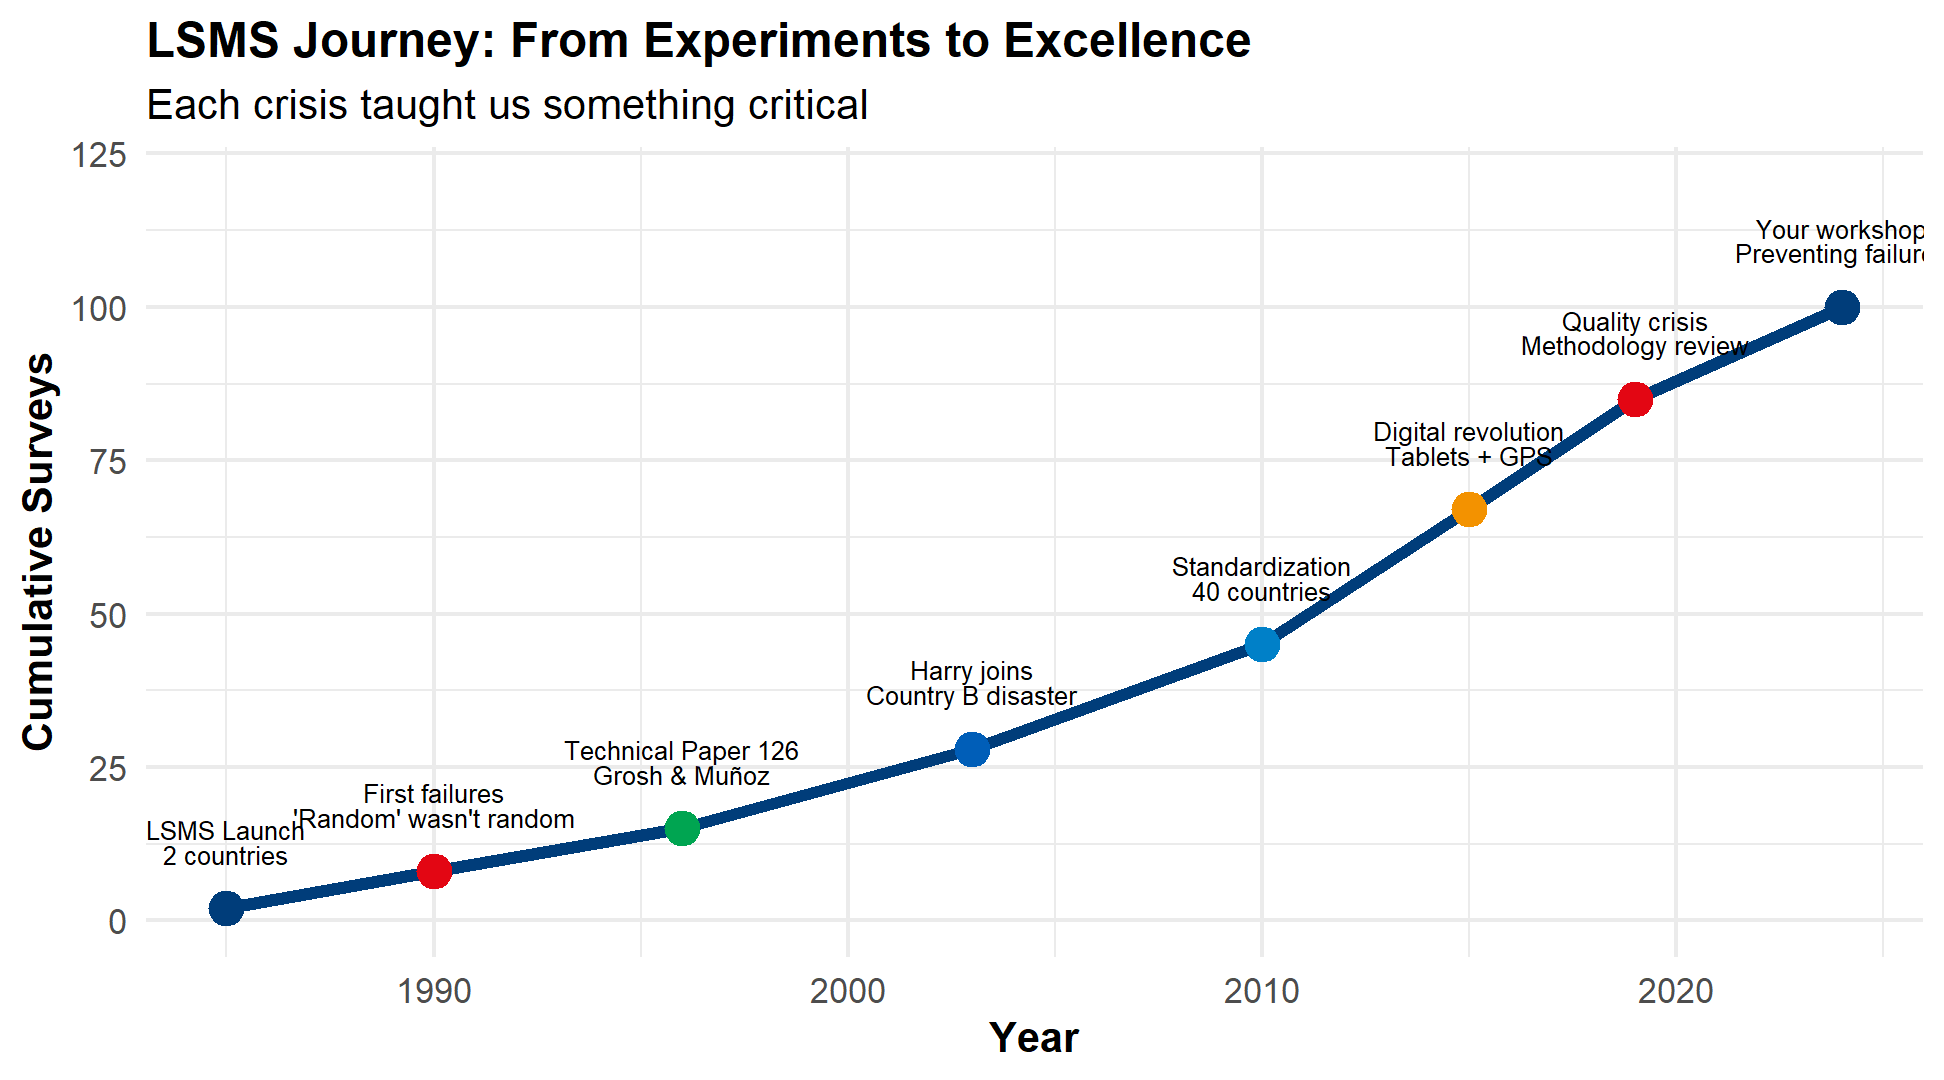
\includegraphics[width=1\linewidth]{Day1_Foundations_International_Standards_files/figure-latex/wb-timeline-1}

\textbf{Key Learning}: Every methodology in Technical Paper 126 came
from a field failure

\begin{center}\rule{0.5\linewidth}{0.5pt}\end{center}

\section{Slide 3: International Challenge Documentation - Real Problems,
Real
Solutions}\label{slide-3-international-challenge-documentation---real-problems-real-solutions}

\subsection{The 2019 Crisis That Changed
Everything}\label{the-2019-crisis-that-changed-everything}

.pull-left{[} \#\#\# What Went Wrong Country C's national survey: -
Design effect = 4.8 (expected 2.0) - Costs 140\% over budget\\
- Results challenged in parliament - International funding suspended

\textbf{Root cause}: Copy-pasted design from different context {]}

.pull-right{[}

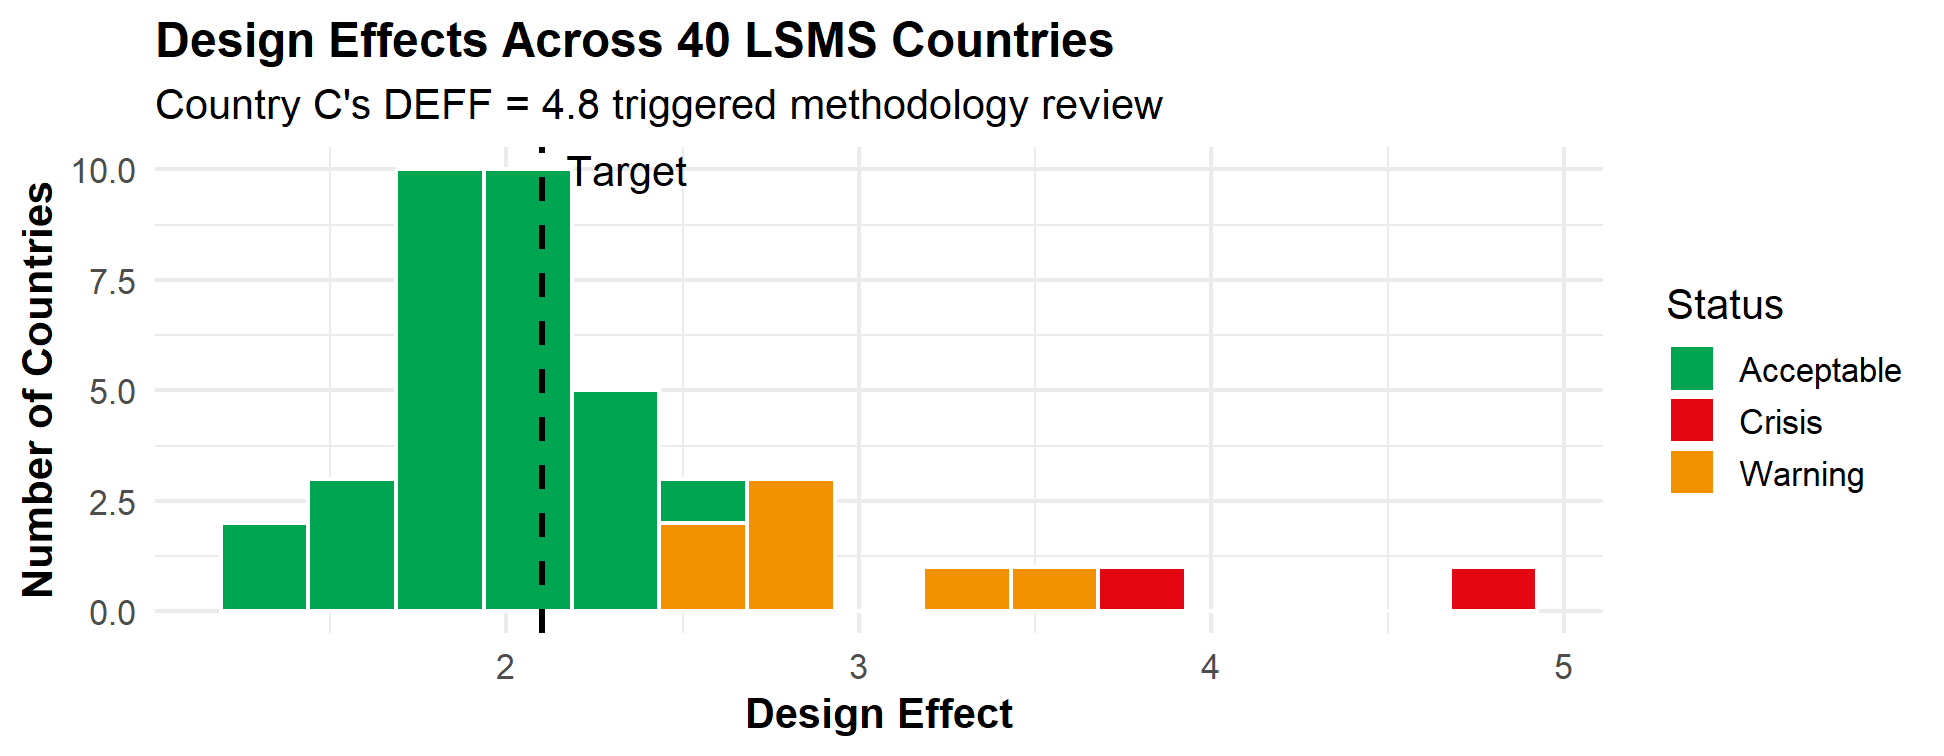
\includegraphics[width=1\linewidth]{Day1_Foundations_International_Standards_files/figure-latex/deff-crisis-1}
{]}

\textbf{Lesson}: One size never fits all - adapt methods to context

\begin{center}\rule{0.5\linewidth}{0.5pt}\end{center}

\section{Slide 4: Eurostat Quality Benchmarks - The Day Brussels
Called}\label{slide-4-eurostat-quality-benchmarks---the-day-brussels-called}

\subsection{``Your Coefficients of Variation Are
Unacceptable''}\label{your-coefficients-of-variation-are-unacceptable}

.pull-left{[} \#\#\# The Regulation \textbf{EU 1177/2003 Article 7}: -
CV must be \textless{} 5\% for key indicators - Quarterly quality
reports mandatory - Non-compliance = funding withdrawal

\textbf{The wake-up call}: Country D lost €2.3M in 2018 {]}

.pull-right{[} \#\#\# Your Current Performance

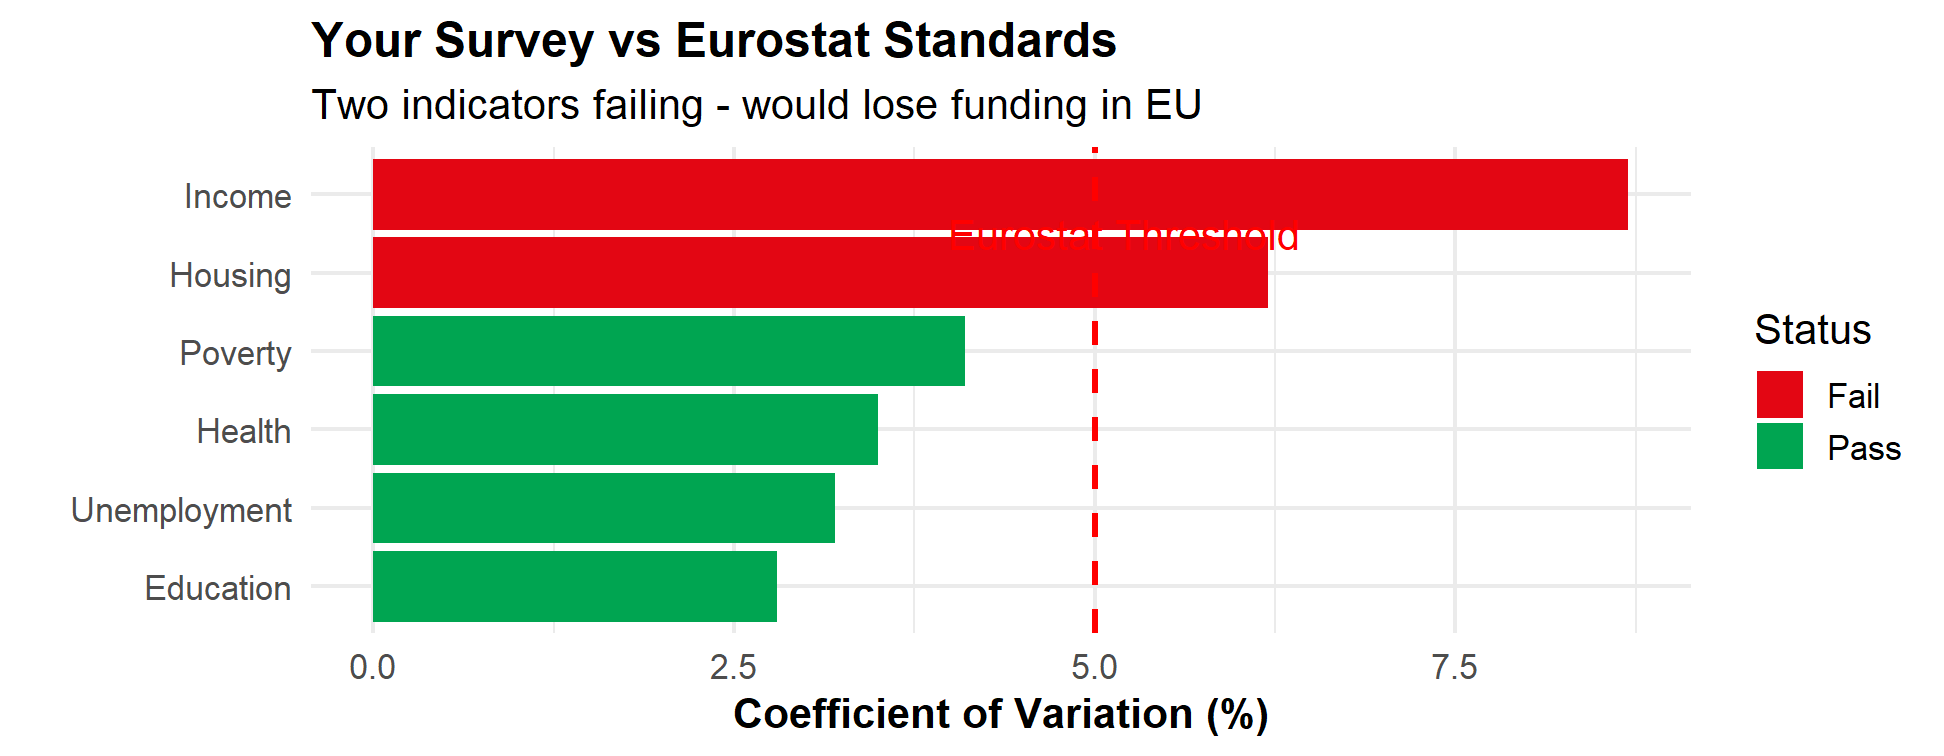
\includegraphics[width=1\linewidth]{Day1_Foundations_International_Standards_files/figure-latex/cv-reality-1}
{]}

\textbf{Monday Morning Question}: What will you tell the Minister about
Income CV = 8.7\%?

\begin{center}\rule{0.5\linewidth}{0.5pt}\end{center}

\section{Slide 5: OECD Standards Application - Minimum Sample Sizes That
Work}\label{slide-5-oecd-standards-application---minimum-sample-sizes-that-work}

\subsection{The Meeting That Changed My
Approach}\label{the-meeting-that-changed-my-approach}

.pull-left{[} \#\#\# Paris, 2013 - OECD Headquarters

\textbf{Their challenge}: \emph{``Harry, prove 500 per domain works''}

My response required: - 73 slides of evidence - 12 country examples - 3
hours of debate

\textbf{The outcome}: OECD Guidelines Chapter 3 {]}

.pull-right{[} \#\#\# The Magic Number Decoded

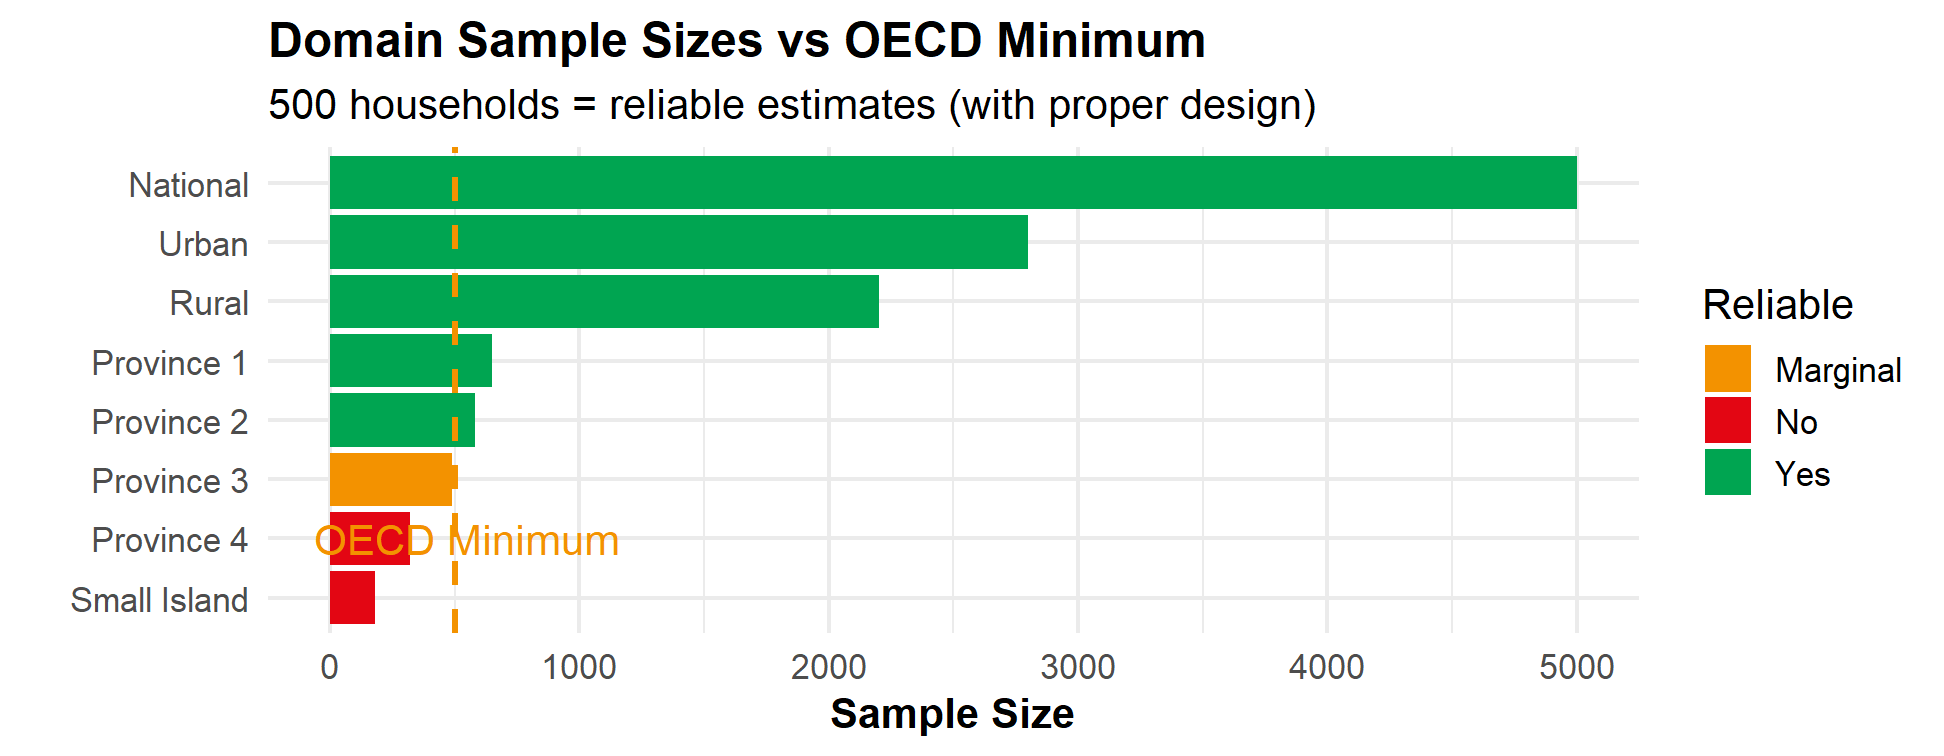
\includegraphics[width=1\linewidth]{Day1_Foundations_International_Standards_files/figure-latex/sample-domains-1}
{]}

\textbf{Real cost}: Below 500, confidence intervals become
``suggestions''

\begin{center}\rule{0.5\linewidth}{0.5pt}\end{center}

\section{Slide 6: Regional Context Analysis - Your Monday Morning
Reality}\label{slide-6-regional-context-analysis---your-monday-morning-reality}

\subsection{Let's Look at YOUR
Metadata}\label{lets-look-at-your-metadata}

.pull-left{[} \#\#\# What You Have ✅ Two-stage stratified design\\
✅ 250 EAs × 20 households = 5,000\\
✅ PPS first stage selection\\
✅ Systematic second stage\\
✅ Three-component weights

\textbf{This follows World Bank LSMS Manual Chapter 3} {]}

.pull-right{[} \#\#\# What This Means

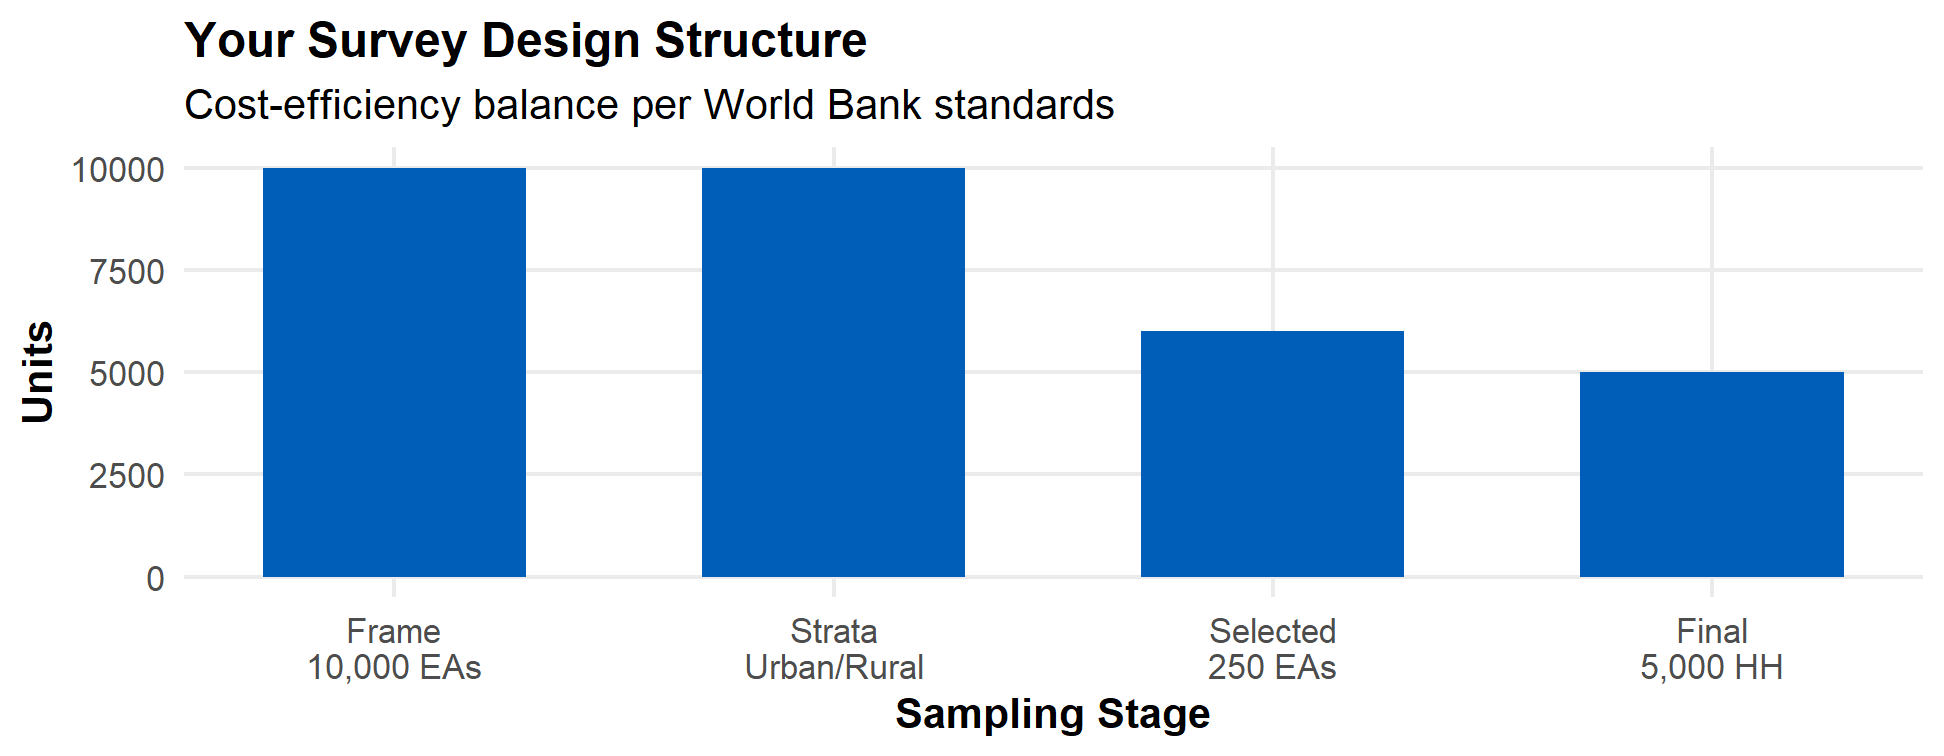
\includegraphics[width=1\linewidth]{Day1_Foundations_International_Standards_files/figure-latex/your-design-1}
{]}

\textbf{The Good News}: Your design is 85\% optimal\\
\textbf{The Challenge}: That remaining 15\% is where problems hide

\begin{center}\rule{0.5\linewidth}{0.5pt}\end{center}

\section{Slide 7: Quality Indicators Observed - The Numbers Don't
Lie}\label{slide-7-quality-indicators-observed---the-numbers-dont-lie}

\subsection{Your Quality Check Results: 95\% Pass
Rate}\label{your-quality-check-results-95-pass-rate}

.pull-left{[} \#\#\# International Benchmarks - \textbf{World Bank}:
90\% minimum ✅ - \textbf{Eurostat}: 93\% threshold ✅\\
- \textbf{UNSD}: Continuous monitoring ✅

You're above all thresholds!

\emph{But wait\ldots{}} {]}

.pull-right{[} \#\#\# Where Problems Hide

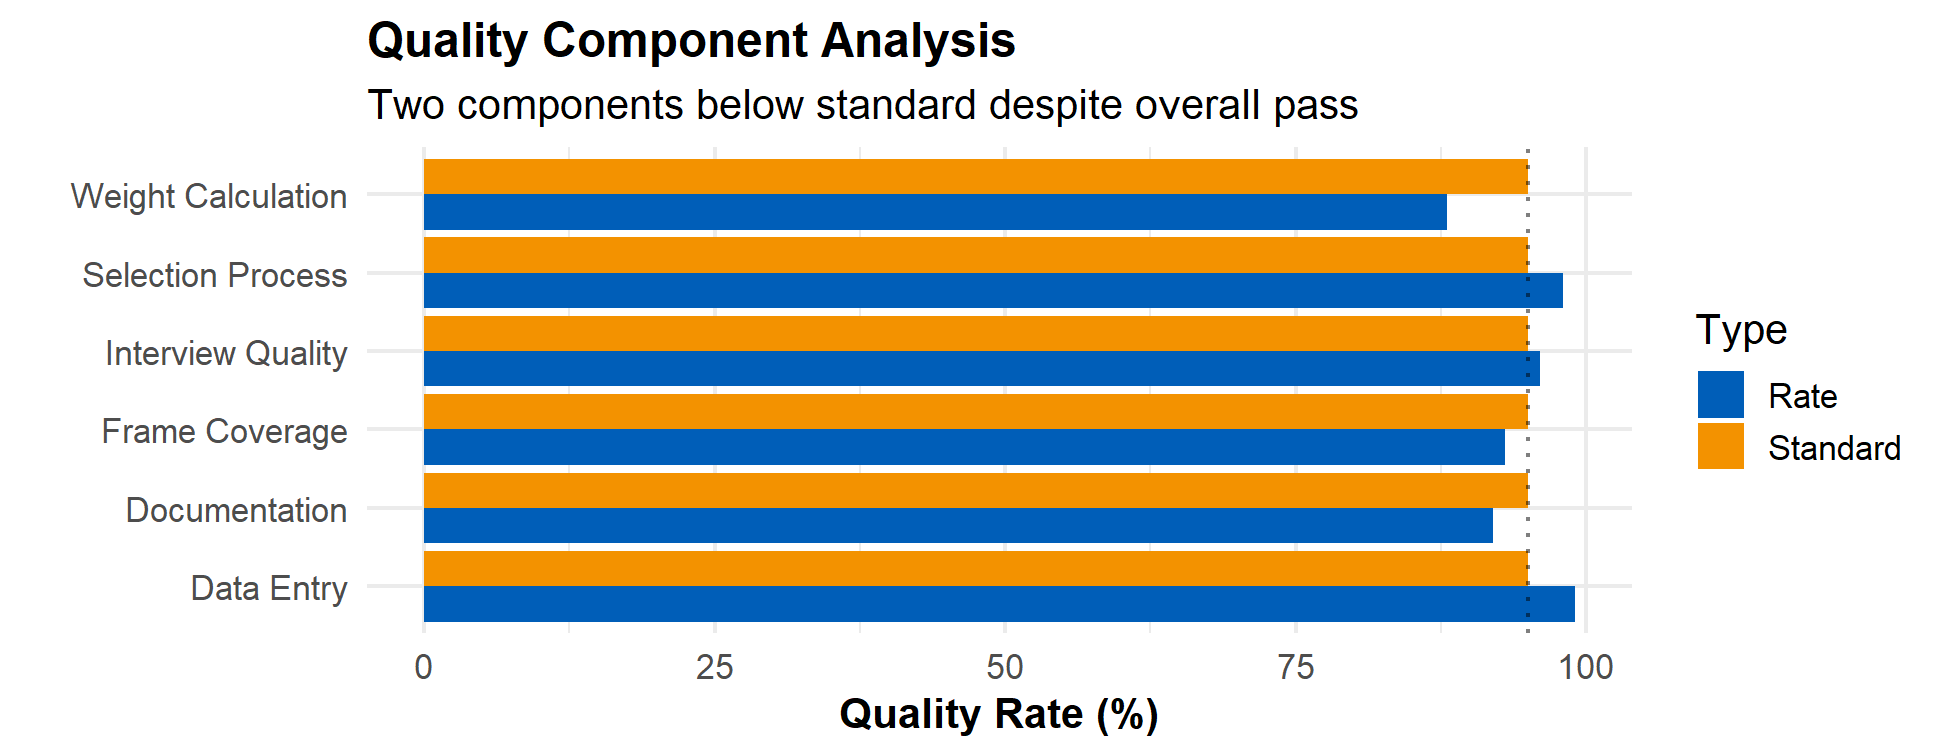
\includegraphics[width=1\linewidth]{Day1_Foundations_International_Standards_files/figure-latex/quality-breakdown-1}
{]}

\textbf{Monday Challenge}: Frame coverage at 93\% means 7\% of
population invisible

\begin{center}\rule{0.5\linewidth}{0.5pt}\end{center}

\section{Slide 8: Module Learning Objectives - Your Transformation
Starts
Now}\label{slide-8-module-learning-objectives---your-transformation-starts-now}

\subsection{By 09:00, You Will Be Able
To:}\label{by-0900-you-will-be-able-to}

.pull-left{[} \#\#\# Immediate Skills ✅ Apply UNSD Fundamental
Principles\\
✅ Implement World Bank LSMS protocols\\
✅ Calculate Eurostat quality indicators\\
✅ Adapt standards to your context

\textbf{More importantly}: Explain to non-statisticians why this matters
{]}

.pull-right{[} \#\#\# Real Outcomes

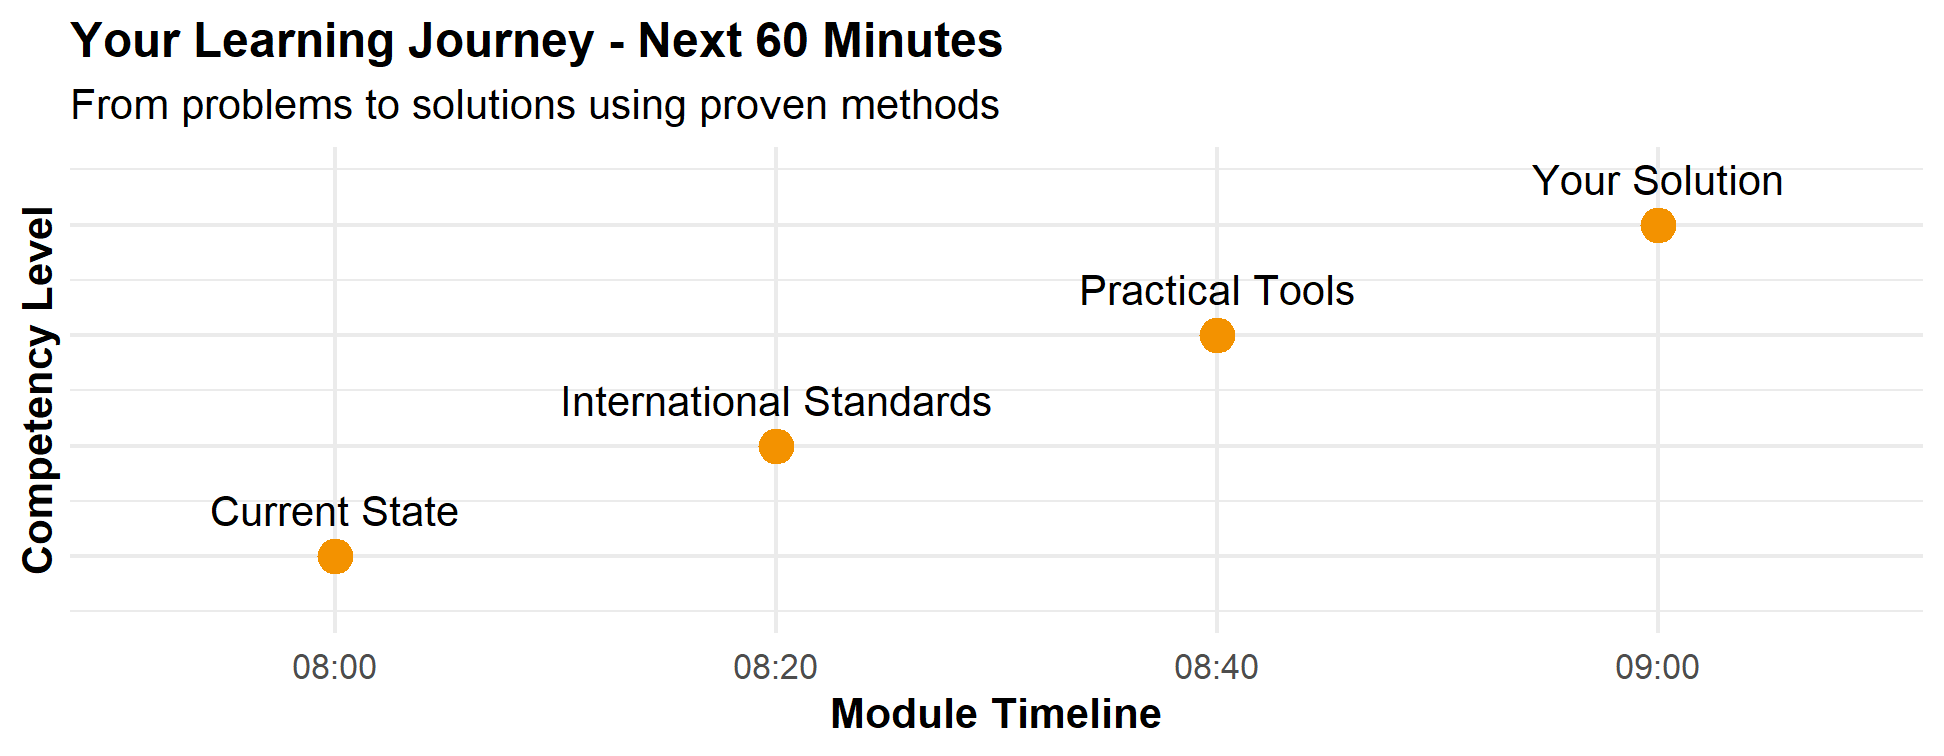
\includegraphics[width=1\linewidth]{Day1_Foundations_International_Standards_files/figure-latex/learning-path-1}
{]}

\textbf{The Promise}: No more Monday morning surprises after today

\begin{center}\rule{0.5\linewidth}{0.5pt}\end{center}

\section{Slide 9: UN Fundamental Principle 1 - Relevance (The
Foundation)}\label{slide-9-un-fundamental-principle-1---relevance-the-foundation}

\subsection{``Official Statistics: Indispensable Element of
Democracy''}\label{official-statistics-indispensable-element-of-democracy}

.pull-left{[} \#\#\# The Principle From UNSD Technical Report F.98:

\emph{``Statistics must balance user needs with resource constraints''}

\textbf{Translation}: You can't measure everything - choose wisely {]}

.pull-right{[} \#\#\# Harry's Reality Check

\textbf{Country E, 2016}: - Ministers wanted 147 indicators - Budget
allowed for 23 - Compromise: 41 critical indicators - Result: Nobody
happy, survey failed

\textbf{Lesson}: Better to measure 20 things well than 100 things poorly
{]}

.center{[} \#\#\# The Monday Morning Test: \emph{``Can you defend every
variable in your questionnaire?''}{]}

\begin{center}\rule{0.5\linewidth}{0.5pt}\end{center}

\section{Slide 10: Implementing Principle 1 - The Stakeholder Matrix
That
Works}\label{slide-10-implementing-principle-1---the-stakeholder-matrix-that-works}

\subsection{World Bank LSMS Manual Section 1.4 -
Operationalized}\label{world-bank-lsms-manual-section-1.4---operationalized}

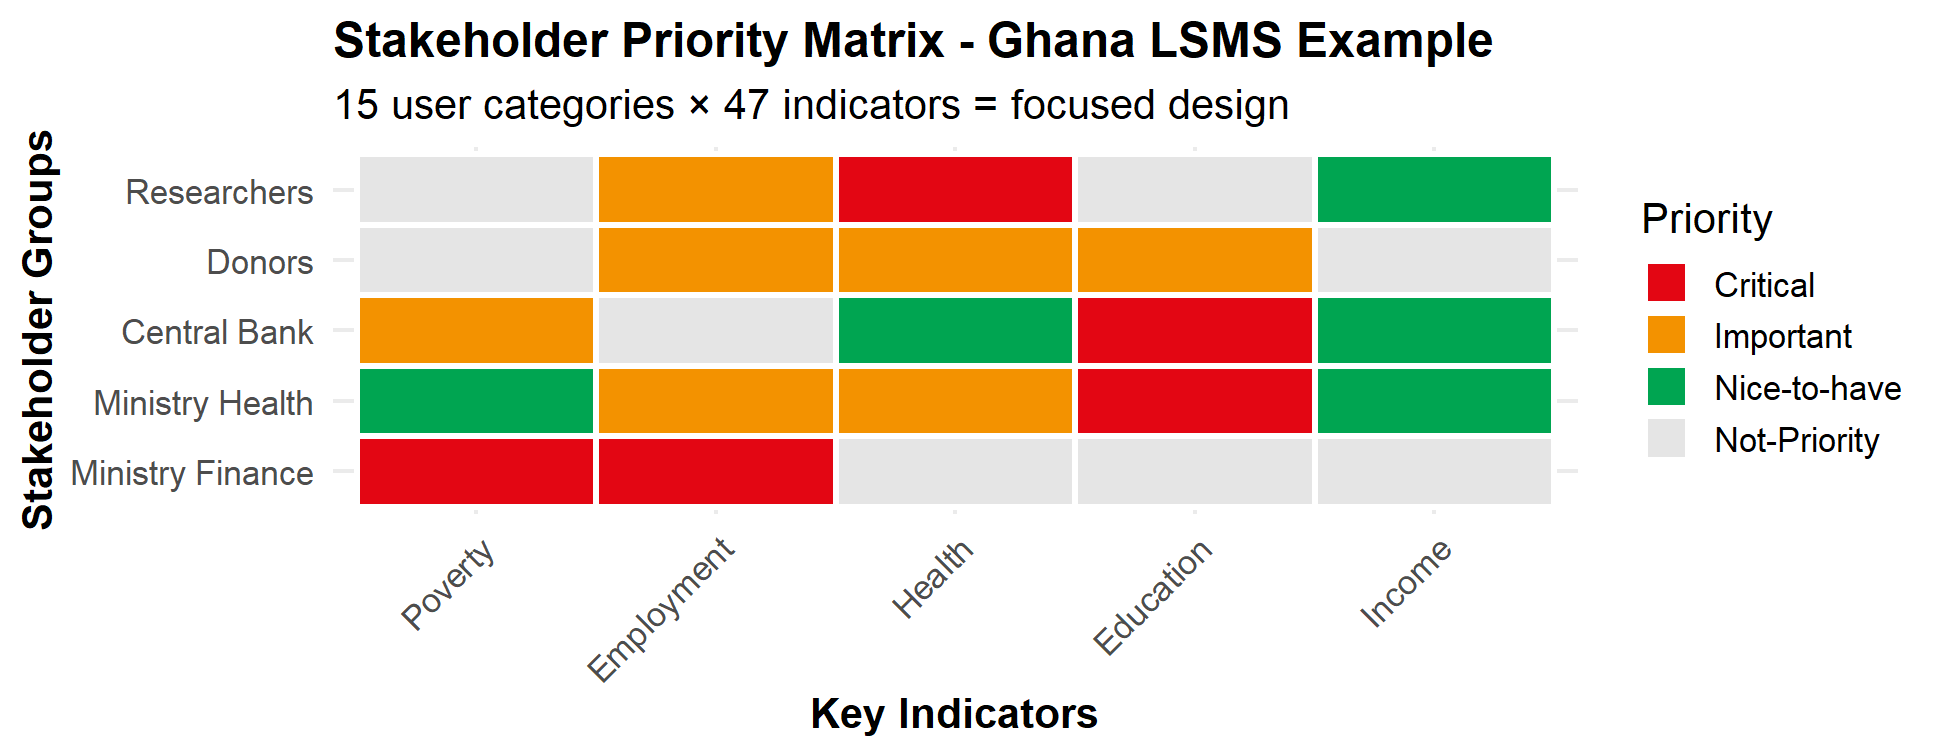
\includegraphics[width=1\linewidth]{Day1_Foundations_International_Standards_files/figure-latex/stakeholder-matrix-1}

\textbf{The Brutal Truth}: If everyone is priority, no one is priority

\begin{center}\rule{0.5\linewidth}{0.5pt}\end{center}

\section{Slide 11: Sample Frame Requirements - The Foundation Everything
Rests
On}\label{slide-11-sample-frame-requirements---the-foundation-everything-rests-on}

\subsection{UNSD Guidelines on Statistical Business Registers (2015)
Chapter
4}\label{unsd-guidelines-on-statistical-business-registers-2015-chapter-4}

.pull-left{[} \#\#\# Frame Quality Dimensions

Your EA master file must have: 1. \textbf{Coverage}: ≥95\% of target
population 2. \textbf{Accuracy}: Correct classifications 3.
\textbf{Timeliness}: Updated within 2 years 4. \textbf{Uniqueness}: No
duplications 5. \textbf{Accessibility}: Usable format {]}

.pull-right{[} \#\#\# Your Frame Reality

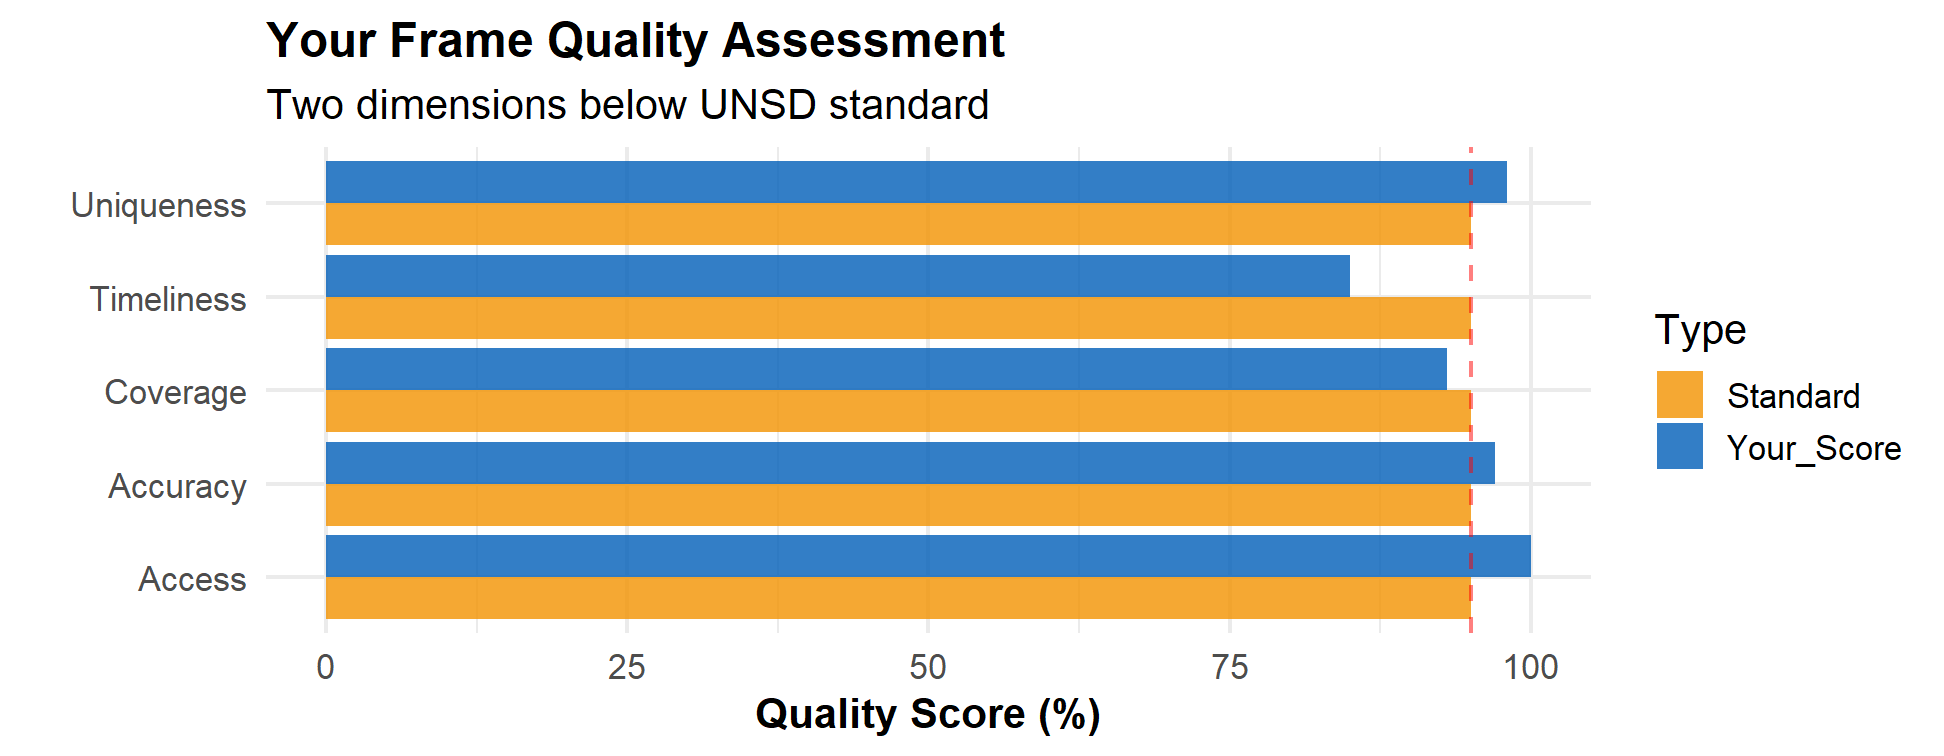
\includegraphics[width=1\linewidth]{Day1_Foundations_International_Standards_files/figure-latex/frame-quality-1}
{]}

\textbf{Coverage at 93\%}: Missing 7\% of population\\
\textbf{Timeliness at 85\%}: Based on 2022 data for 2024 survey

\begin{center}\rule{0.5\linewidth}{0.5pt}\end{center}

\section{Slide 12: World Bank Frame Assessment Tool - Let's Calculate
Together}\label{slide-12-world-bank-frame-assessment-tool---lets-calculate-together}

\subsection{LSMS Frame\_Quality\_Assessment.xlsx
Template}\label{lsms-frame_quality_assessment.xlsx-template}

\begin{Shaded}
\begin{Highlighting}[]
\CommentTok{\# Live calculation of frame coverage}
\CommentTok{\# This is what you\textquotesingle{}ll do with real data}

\CommentTok{\# Your frame statistics}
\NormalTok{frame\_units }\OtherTok{\textless{}{-}} \DecValTok{10000}  \CommentTok{\# Total EAs in frame}
\NormalTok{census\_units }\OtherTok{\textless{}{-}} \DecValTok{10753}  \CommentTok{\# True number from census projection}
\NormalTok{duplicates }\OtherTok{\textless{}{-}} \DecValTok{120}     \CommentTok{\# Identified duplicates}
\NormalTok{outdated }\OtherTok{\textless{}{-}} \DecValTok{633}       \CommentTok{\# Units needing update}

\CommentTok{\# Calculate quality metrics}
\NormalTok{coverage\_rate }\OtherTok{\textless{}{-}}\NormalTok{ (frame\_units }\SpecialCharTok{/}\NormalTok{ census\_units) }\SpecialCharTok{*} \DecValTok{100}
\NormalTok{duplication\_rate }\OtherTok{\textless{}{-}}\NormalTok{ (duplicates }\SpecialCharTok{/}\NormalTok{ frame\_units) }\SpecialCharTok{*} \DecValTok{100}
\NormalTok{currency\_rate }\OtherTok{\textless{}{-}}\NormalTok{ ((frame\_units }\SpecialCharTok{{-}}\NormalTok{ outdated) }\SpecialCharTok{/}\NormalTok{ frame\_units) }\SpecialCharTok{*} \DecValTok{100}

\CommentTok{\# Display results}
\FunctionTok{cat}\NormalTok{(}\StringTok{"Coverage Rate:"}\NormalTok{, }\FunctionTok{round}\NormalTok{(coverage\_rate, }\DecValTok{1}\NormalTok{), }\StringTok{"\%}\SpecialCharTok{\textbackslash{}n}\StringTok{"}\NormalTok{)}
\end{Highlighting}
\end{Shaded}

\begin{verbatim}
## Coverage Rate: 93 %
\end{verbatim}

\begin{Shaded}
\begin{Highlighting}[]
\FunctionTok{cat}\NormalTok{(}\StringTok{"Duplication Rate:"}\NormalTok{, }\FunctionTok{round}\NormalTok{(duplication\_rate, }\DecValTok{1}\NormalTok{), }\StringTok{"\%}\SpecialCharTok{\textbackslash{}n}\StringTok{"}\NormalTok{)}
\end{Highlighting}
\end{Shaded}

\begin{verbatim}
## Duplication Rate: 1.2 %
\end{verbatim}

\begin{Shaded}
\begin{Highlighting}[]
\FunctionTok{cat}\NormalTok{(}\StringTok{"Currency Rate:"}\NormalTok{, }\FunctionTok{round}\NormalTok{(currency\_rate, }\DecValTok{1}\NormalTok{), }\StringTok{"\%}\SpecialCharTok{\textbackslash{}n}\StringTok{"}\NormalTok{)}
\end{Highlighting}
\end{Shaded}

\begin{verbatim}
## Currency Rate: 93.7 %
\end{verbatim}

\textbf{Nicaragua LSMS Example}: Started at 87\%, improved to 94.3\%
after update

\begin{center}\rule{0.5\linewidth}{0.5pt}\end{center}

\section{Slide 13: Stratification Following International Standards -
The Power of
Groups}\label{slide-13-stratification-following-international-standards---the-power-of-groups}

\subsection{Eurostat Handbook on Precision Requirements (2023) Equation
2.7}\label{eurostat-handbook-on-precision-requirements-2023-equation-2.7}

.pull-left{[} \#\#\# Optimal Allocation Formula

\[n_h = n \times \frac{N_h \times S_h}{\sum(N_h \times S_h)}\]

Where: - \(n_h\) = sample in stratum h - \(N_h\) = population in stratum
h\\
- \(S_h\) = standard deviation in h {]}

.pull-right{[} \#\#\# Your Stratification Impact

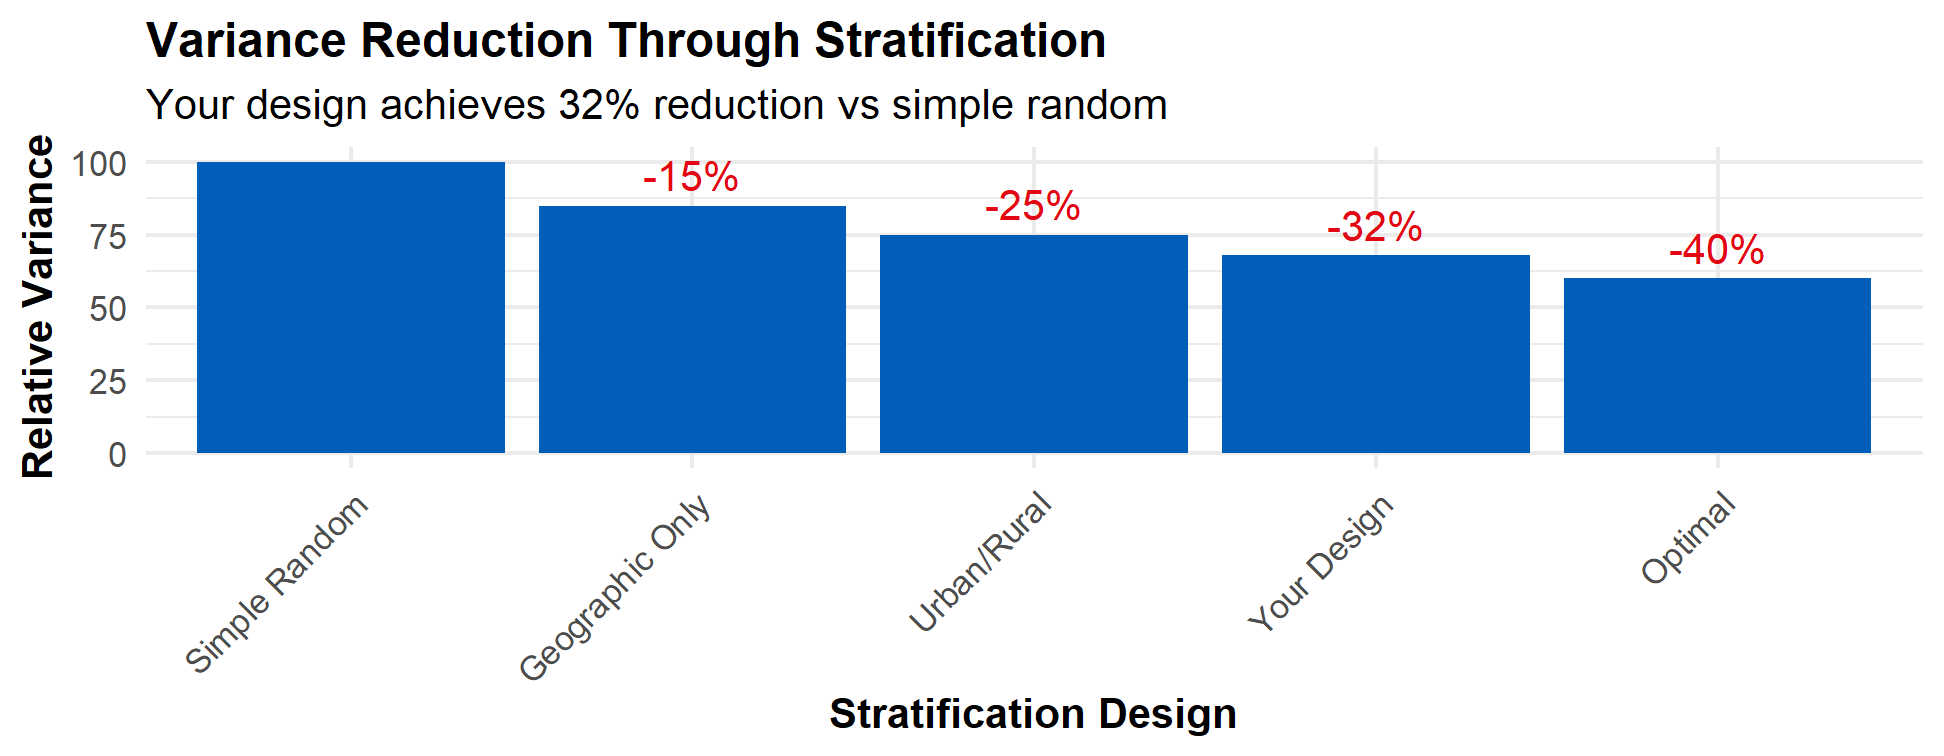
\includegraphics[width=1\linewidth]{Day1_Foundations_International_Standards_files/figure-latex/stratification-impact-1}
{]}

\textbf{Monday Reality}: Good stratification = smaller samples = lower
costs

\begin{center}\rule{0.5\linewidth}{0.5pt}\end{center}

\section{Slide 14: Calculating Optimal Allocation - Real Numbers, Real
Impact}\label{slide-14-calculating-optimal-allocation---real-numbers-real-impact}

\subsection{Using World Bank Formula from Technical Paper 126, Page
45}\label{using-world-bank-formula-from-technical-paper-126-page-45}

\begin{Shaded}
\begin{Highlighting}[]
\CommentTok{\# Live calculation {-} you\textquotesingle{}ll do this with your data}
\CommentTok{\# Stratum data (example from your survey)}
\NormalTok{strata\_data }\OtherTok{\textless{}{-}} \FunctionTok{data.frame}\NormalTok{(}
  \AttributeTok{Stratum =} \FunctionTok{c}\NormalTok{(}\StringTok{"Urban"}\NormalTok{, }\StringTok{"Rural"}\NormalTok{),}
  \AttributeTok{N =} \FunctionTok{c}\NormalTok{(}\DecValTok{4000}\NormalTok{, }\DecValTok{6000}\NormalTok{),  }\CommentTok{\# Population sizes}
  \AttributeTok{S =} \FunctionTok{c}\NormalTok{(}\FloatTok{12.5}\NormalTok{, }\FloatTok{8.3}\NormalTok{)    }\CommentTok{\# Standard deviations}
\NormalTok{)}

\CommentTok{\# Calculate optimal allocation for n = 250 PSUs}
\NormalTok{strata\_data }\OtherTok{\textless{}{-}}\NormalTok{ strata\_data }\SpecialCharTok{\%\textgreater{}\%}
  \FunctionTok{mutate}\NormalTok{(}
    \AttributeTok{N\_times\_S =}\NormalTok{ N }\SpecialCharTok{*}\NormalTok{ S,}
    \AttributeTok{Allocation =} \FunctionTok{round}\NormalTok{(}\DecValTok{250} \SpecialCharTok{*}\NormalTok{ N\_times\_S }\SpecialCharTok{/} \FunctionTok{sum}\NormalTok{(N\_times\_S))}
\NormalTok{  )}

\FunctionTok{print}\NormalTok{(strata\_data)}
\end{Highlighting}
\end{Shaded}

\begin{verbatim}
##   Stratum    N    S N_times_S Allocation
## 1   Urban 4000 12.5     50000        125
## 2   Rural 6000  8.3     49800        125
\end{verbatim}

\textbf{Result}: Urban gets more samples despite smaller population due
to higher variance

\begin{center}\rule{0.5\linewidth}{0.5pt}\end{center}

\section{Slide 15: Two-Stage Design Efficiency - Why It
Works}\label{slide-15-two-stage-design-efficiency---why-it-works}

\subsection{UNSD Technical Report F.98 Section 3.4
Analysis}\label{unsd-technical-report-f.98-section-3.4-analysis}

.pull-left{[} \#\#\# The Cost-Variance Tradeoff

For fixed budget, optimize: \[m\sqrt{n}\]

Where: - m = number of PSUs - n = elements per PSU

Your design: 250 × 20 = 5,000 {]}

.pull-right{[} \#\#\# Efficiency Comparison

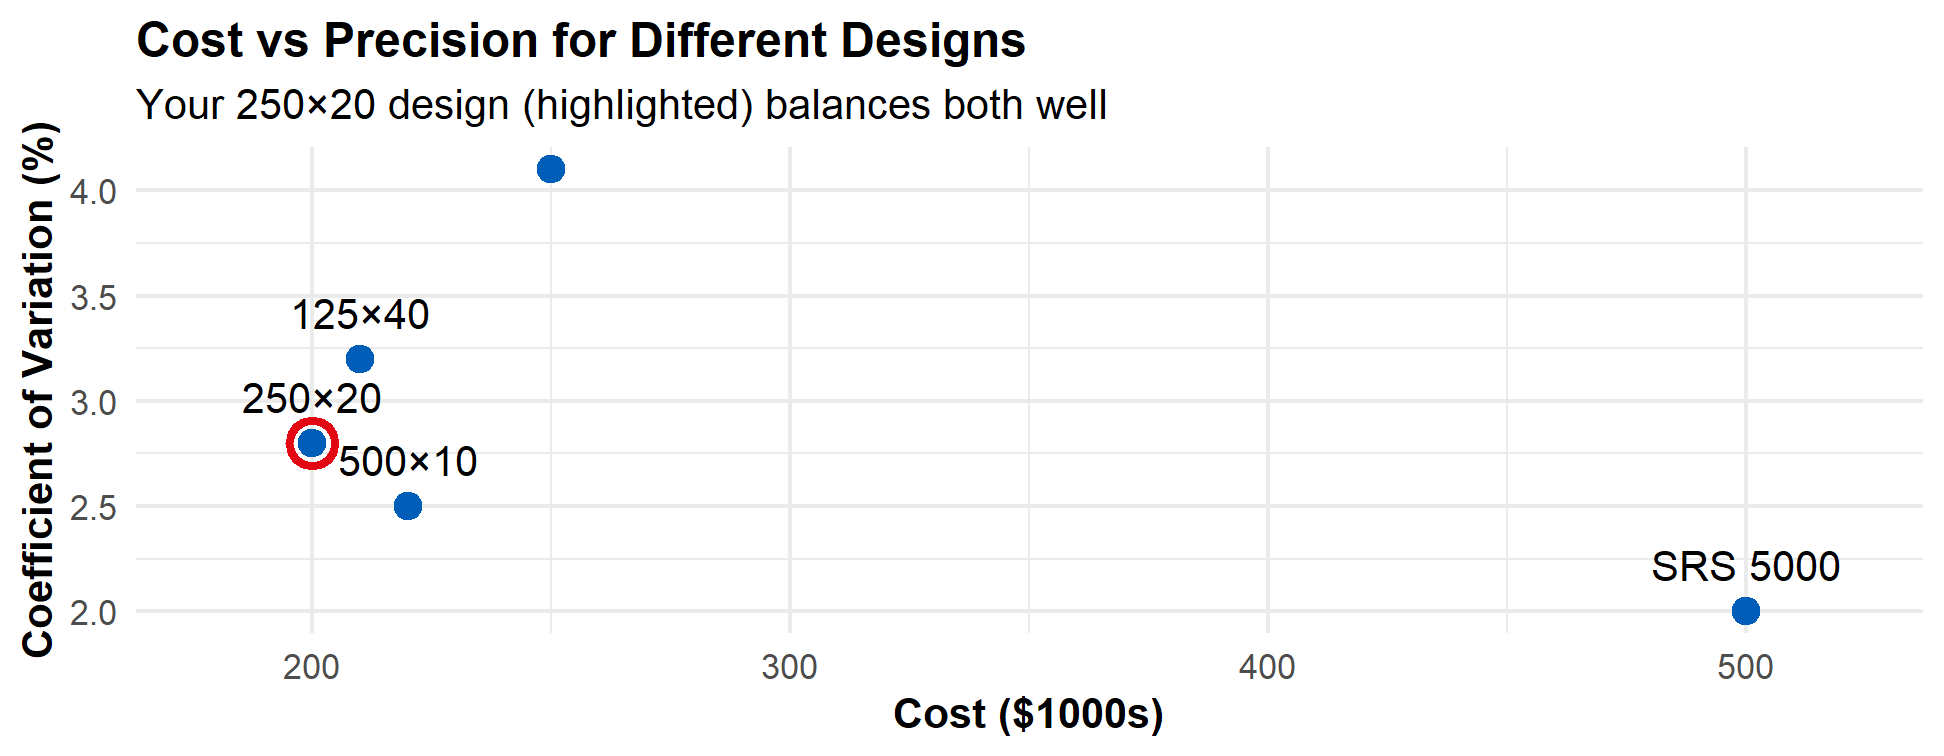
\includegraphics[width=1\linewidth]{Day1_Foundations_International_Standards_files/figure-latex/two-stage-efficiency-1}
{]}

\textbf{Your design} achieves 60\% cost savings with only 40\% precision
loss

\begin{center}\rule{0.5\linewidth}{0.5pt}\end{center}

\section{Slide 16: PSU Selection Procedures - Getting PPS
Right}\label{slide-16-psu-selection-procedures---getting-pps-right}

\subsection{World Bank LSMS Manual Chapter 3.2 - The Critical First
Stage}\label{world-bank-lsms-manual-chapter-3.2---the-critical-first-stage}

.pull-left{[} \#\#\# Systematic PPS Algorithm

\begin{enumerate}
\def\labelenumi{\arabic{enumi}.}
\tightlist
\item
  List all PSUs with sizes
\item
  Calculate cumulative sizes
\item
  Determine interval k = ΣSize/n
\item
  Random start r between 1 and k
\item
  Select at r, r+k, r+2k, \ldots{}
\end{enumerate}

\textbf{Your implementation}: ✅ Correct {]}

.pull-right{[} \#\#\# Visual Example

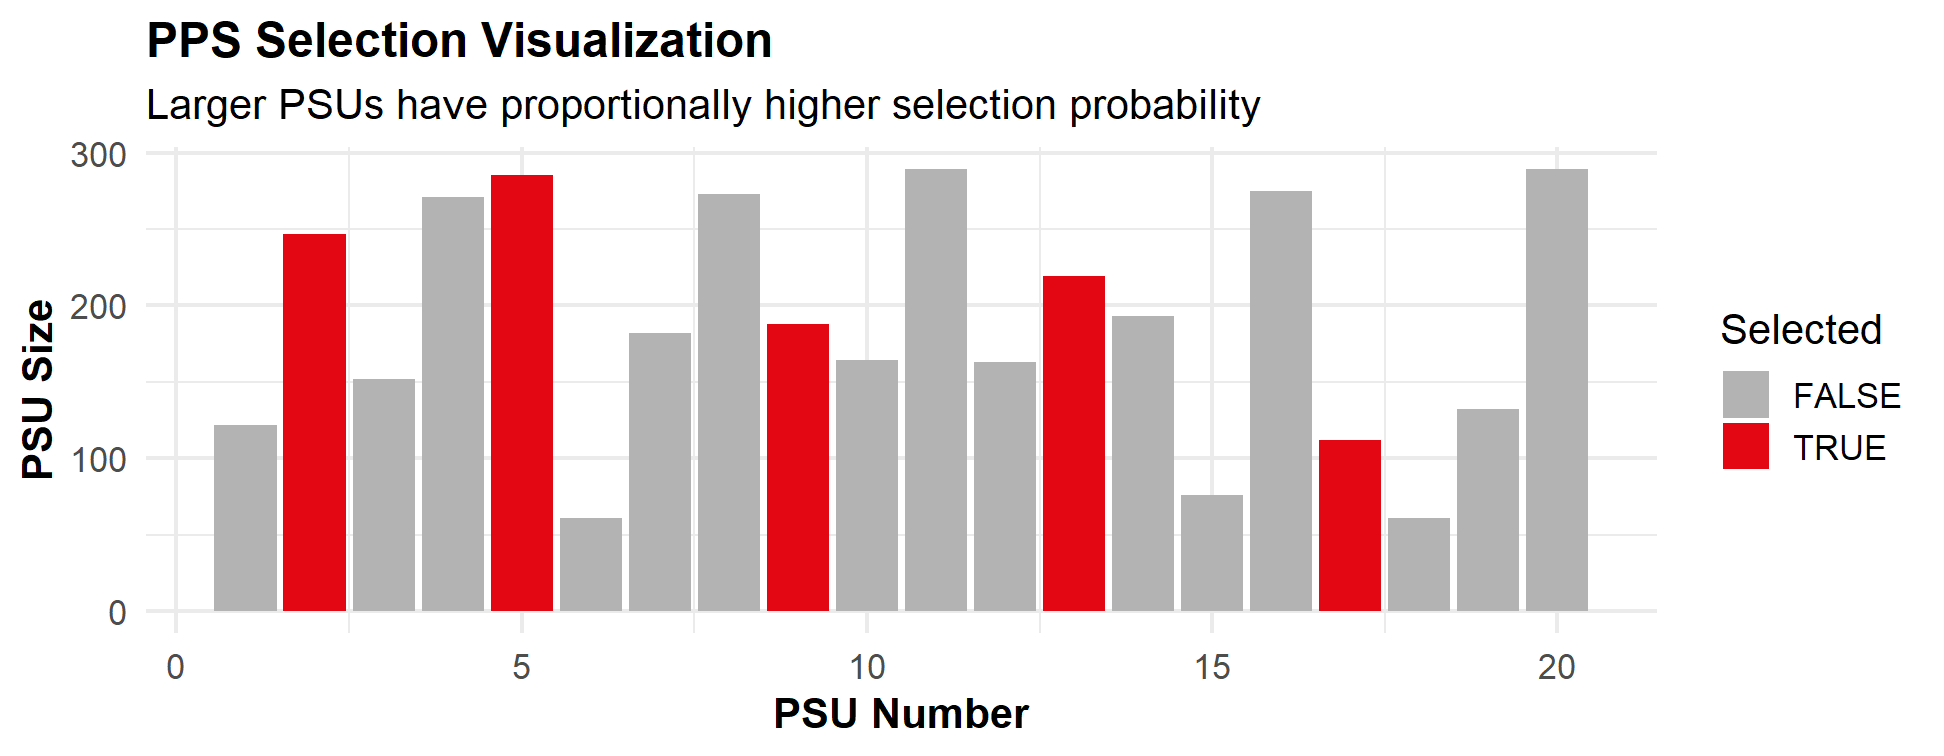
\includegraphics[width=1\linewidth]{Day1_Foundations_International_Standards_files/figure-latex/pps-selection-1}
{]}

\textbf{Critical}: Document your random start for reproducibility

\begin{center}\rule{0.5\linewidth}{0.5pt}\end{center}

\section{Slide 17: Within-PSU Selection Standards - The Second
Stage}\label{slide-17-within-psu-selection-standards---the-second-stage}

\subsection{Eurostat Guidelines: Systematic with Random
Start}\label{eurostat-guidelines-systematic-with-random-start}

.pull-left{[} \#\#\# Why 20 Households?

Cost-variance optimization:

\begin{Shaded}
\begin{Highlighting}[]
\CommentTok{\# Optimal cluster size calculation}
\NormalTok{c1 }\OtherTok{\textless{}{-}} \DecValTok{100}  \CommentTok{\# PSU cost}
\NormalTok{c2 }\OtherTok{\textless{}{-}} \DecValTok{5}    \CommentTok{\# Element cost  }
\NormalTok{rho }\OtherTok{\textless{}{-}} \FloatTok{0.05}  \CommentTok{\# Intraclass correlation}

\NormalTok{b\_optimal }\OtherTok{\textless{}{-}} \FunctionTok{sqrt}\NormalTok{((c1}\SpecialCharTok{/}\NormalTok{c2) }\SpecialCharTok{*}\NormalTok{ (}\DecValTok{1}\SpecialCharTok{{-}}\NormalTok{rho)}\SpecialCharTok{/}\NormalTok{rho)}
\FunctionTok{print}\NormalTok{(}\FunctionTok{paste}\NormalTok{(}\StringTok{"Optimal cluster size:"}\NormalTok{, }
            \FunctionTok{round}\NormalTok{(b\_optimal)))}
\end{Highlighting}
\end{Shaded}

\begin{verbatim}
## [1] "Optimal cluster size: 19"
\end{verbatim}

Your choice of 20 is near-optimal! {]}

.pull-right{[} \#\#\# Selection Pattern

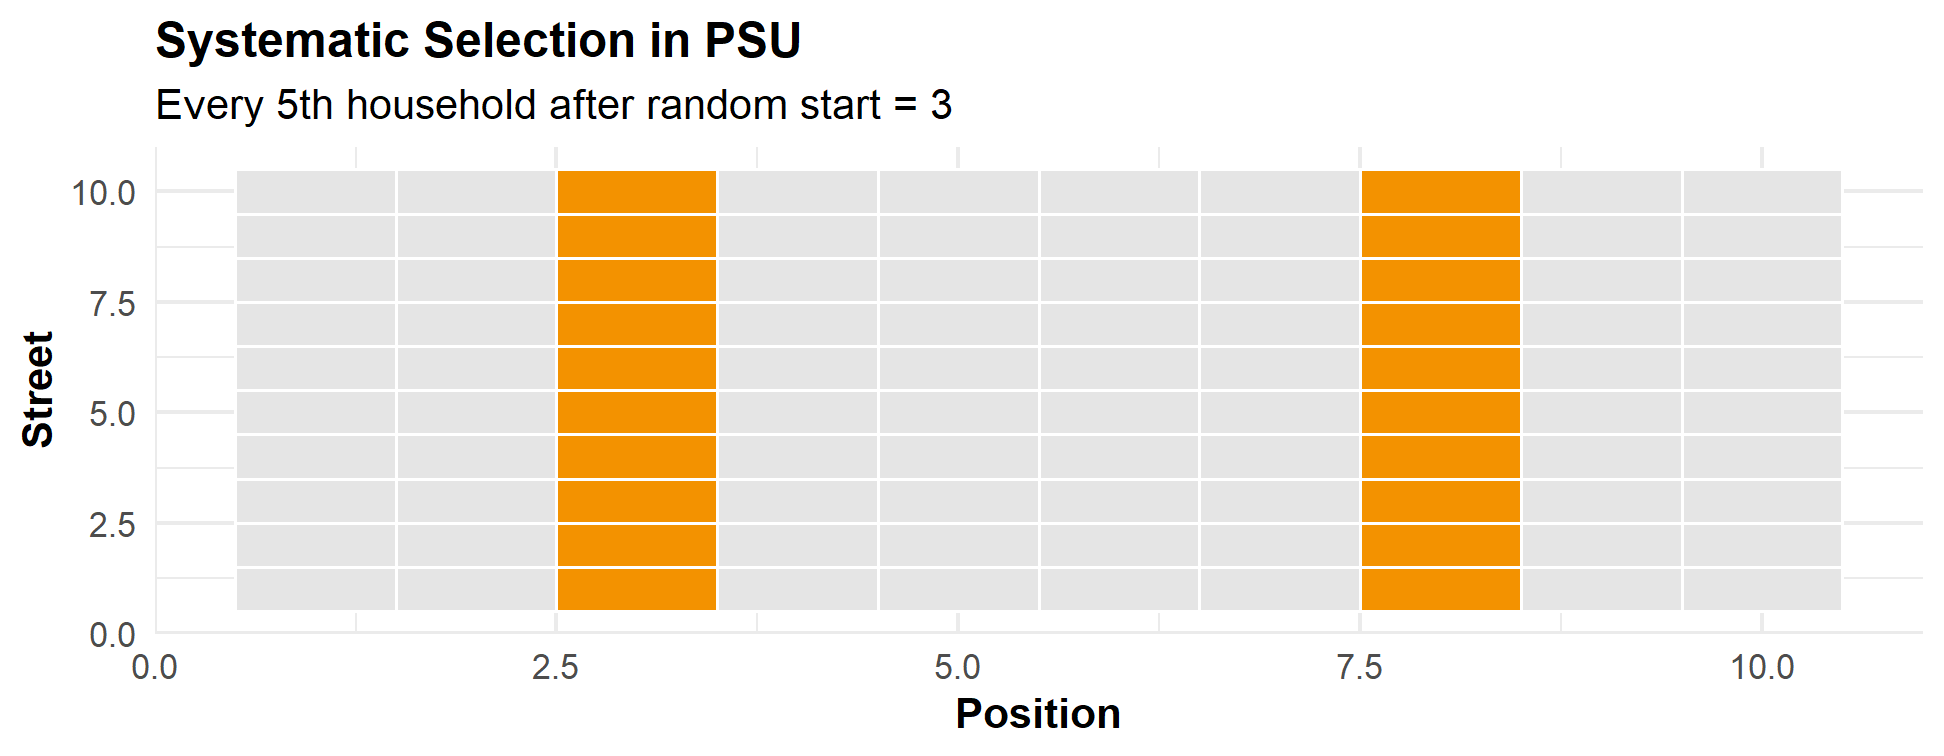
\includegraphics[width=1\linewidth]{Day1_Foundations_International_Standards_files/figure-latex/systematic-pattern-1}
{]}

\textbf{Field advantage}: Enumerators can verify selection visually

\begin{center}\rule{0.5\linewidth}{0.5pt}\end{center}

\section{Slide 18: Sample Size Determination - The Mathematics of
Precision}\label{slide-18-sample-size-determination---the-mathematics-of-precision}

\subsection{World Bank's Enhanced Formula with Design
Effect}\label{world-banks-enhanced-formula-with-design-effect}

.pull-left{[} \#\#\# The Calculation

\[n = DEFF \times \frac{z^2 \times p(1-p)}{e^2}\]

For your survey: - DEFF = 1.68 (calculated) - z = 1.96 (95\% confidence)
- p = 0.5 (maximum variance) - e = 0.028 (your precision) {]}

.pull-right{[}

\begin{Shaded}
\begin{Highlighting}[]
\CommentTok{\# Your actual sample size calculation}
\NormalTok{DEFF }\OtherTok{\textless{}{-}} \FloatTok{1.68}
\NormalTok{z }\OtherTok{\textless{}{-}} \FloatTok{1.96}
\NormalTok{p }\OtherTok{\textless{}{-}} \FloatTok{0.5}
\NormalTok{e }\OtherTok{\textless{}{-}} \FloatTok{0.028}

\NormalTok{n\_simple }\OtherTok{\textless{}{-}}\NormalTok{ (z}\SpecialCharTok{\^{}}\DecValTok{2} \SpecialCharTok{*}\NormalTok{ p }\SpecialCharTok{*}\NormalTok{ (}\DecValTok{1}\SpecialCharTok{{-}}\NormalTok{p)) }\SpecialCharTok{/}\NormalTok{ e}\SpecialCharTok{\^{}}\DecValTok{2}
\NormalTok{n\_complex }\OtherTok{\textless{}{-}}\NormalTok{ DEFF }\SpecialCharTok{*}\NormalTok{ n\_simple}

\FunctionTok{cat}\NormalTok{(}\StringTok{"Simple Random Sample:"}\NormalTok{, }\FunctionTok{round}\NormalTok{(n\_simple), }\StringTok{"}\SpecialCharTok{\textbackslash{}n}\StringTok{"}\NormalTok{)}
\end{Highlighting}
\end{Shaded}

\begin{verbatim}
## Simple Random Sample: 1225
\end{verbatim}

\begin{Shaded}
\begin{Highlighting}[]
\FunctionTok{cat}\NormalTok{(}\StringTok{"With Design Effect:"}\NormalTok{, }\FunctionTok{round}\NormalTok{(n\_complex), }\StringTok{"}\SpecialCharTok{\textbackslash{}n}\StringTok{"}\NormalTok{)}
\end{Highlighting}
\end{Shaded}

\begin{verbatim}
## With Design Effect: 2058
\end{verbatim}

\begin{Shaded}
\begin{Highlighting}[]
\FunctionTok{cat}\NormalTok{(}\StringTok{"Your Actual Sample:"}\NormalTok{, }\DecValTok{5000}\NormalTok{, }\StringTok{"}\SpecialCharTok{\textbackslash{}n}\StringTok{"}\NormalTok{)}
\end{Highlighting}
\end{Shaded}

\begin{verbatim}
## Your Actual Sample: 5000
\end{verbatim}

\begin{Shaded}
\begin{Highlighting}[]
\FunctionTok{cat}\NormalTok{(}\StringTok{"Safety Margin:"}\NormalTok{, }\FunctionTok{round}\NormalTok{(}\DecValTok{5000} \SpecialCharTok{{-}}\NormalTok{ n\_complex), }\StringTok{"households"}\NormalTok{)}
\end{Highlighting}
\end{Shaded}

\begin{verbatim}
## Safety Margin: 2942 households
\end{verbatim}

{]}

\textbf{Good news}: Your 5,000 provides buffer for non-response

\begin{center}\rule{0.5\linewidth}{0.5pt}\end{center}

\section{Slide 19: Design Effect Estimation - Understanding Your
1.68}\label{slide-19-design-effect-estimation---understanding-your-1.68}

\subsection{Eurostat Formula: DEFF = 1 +
δ(b-1)}\label{eurostat-formula-deff-1-ux3b4b-1}

\begin{Shaded}
\begin{Highlighting}[]
\CommentTok{\# Breaking down your design effect}
\CommentTok{\# Component 1: Clustering}
\NormalTok{b }\OtherTok{\textless{}{-}} \DecValTok{20}  \CommentTok{\# cluster size}
\NormalTok{rho }\OtherTok{\textless{}{-}} \FloatTok{0.05}  \CommentTok{\# typical ICC for income}
\NormalTok{DEFF\_cluster }\OtherTok{\textless{}{-}} \DecValTok{1} \SpecialCharTok{+}\NormalTok{ rho }\SpecialCharTok{*}\NormalTok{ (b }\SpecialCharTok{{-}} \DecValTok{1}\NormalTok{)}

\CommentTok{\# Component 2: Stratification benefit  }
\NormalTok{DEFF\_strat }\OtherTok{\textless{}{-}} \FloatTok{0.85}  \CommentTok{\# from variance analysis}

\CommentTok{\# Component 3: Unequal weights}
\NormalTok{cv\_weights }\OtherTok{\textless{}{-}} \FloatTok{0.35}
\NormalTok{DEFF\_weights }\OtherTok{\textless{}{-}} \DecValTok{1} \SpecialCharTok{+}\NormalTok{ cv\_weights}\SpecialCharTok{\^{}}\DecValTok{2}

\CommentTok{\# Total design effect}
\NormalTok{DEFF\_total }\OtherTok{\textless{}{-}}\NormalTok{ DEFF\_cluster }\SpecialCharTok{*}\NormalTok{ DEFF\_strat }\SpecialCharTok{*}\NormalTok{ DEFF\_weights}

\FunctionTok{cat}\NormalTok{(}\StringTok{"Clustering effect:"}\NormalTok{, }\FunctionTok{round}\NormalTok{(DEFF\_cluster, }\DecValTok{2}\NormalTok{), }\StringTok{"}\SpecialCharTok{\textbackslash{}n}\StringTok{"}\NormalTok{)}
\end{Highlighting}
\end{Shaded}

\begin{verbatim}
## Clustering effect: 1.95
\end{verbatim}

\begin{Shaded}
\begin{Highlighting}[]
\FunctionTok{cat}\NormalTok{(}\StringTok{"Stratification benefit:"}\NormalTok{, }\FunctionTok{round}\NormalTok{(DEFF\_strat, }\DecValTok{2}\NormalTok{), }\StringTok{"}\SpecialCharTok{\textbackslash{}n}\StringTok{"}\NormalTok{)}
\end{Highlighting}
\end{Shaded}

\begin{verbatim}
## Stratification benefit: 0.85
\end{verbatim}

\begin{Shaded}
\begin{Highlighting}[]
\FunctionTok{cat}\NormalTok{(}\StringTok{"Weight variation:"}\NormalTok{, }\FunctionTok{round}\NormalTok{(DEFF\_weights, }\DecValTok{2}\NormalTok{), }\StringTok{"}\SpecialCharTok{\textbackslash{}n}\StringTok{"}\NormalTok{)}
\end{Highlighting}
\end{Shaded}

\begin{verbatim}
## Weight variation: 1.12
\end{verbatim}

\begin{Shaded}
\begin{Highlighting}[]
\FunctionTok{cat}\NormalTok{(}\StringTok{"Total DEFF:"}\NormalTok{, }\FunctionTok{round}\NormalTok{(DEFF\_total, }\DecValTok{2}\NormalTok{))}
\end{Highlighting}
\end{Shaded}

\begin{verbatim}
## Total DEFF: 1.86
\end{verbatim}

\textbf{Interpretation}: Clustering hurts, stratification helps, weights
manageable

\begin{center}\rule{0.5\linewidth}{0.5pt}\end{center}

\section{Slide 20: International Benchmarks Applied - How You
Compare}\label{slide-20-international-benchmarks-applied---how-you-compare}

\subsection{Your Design vs Global
Standards}\label{your-design-vs-global-standards}

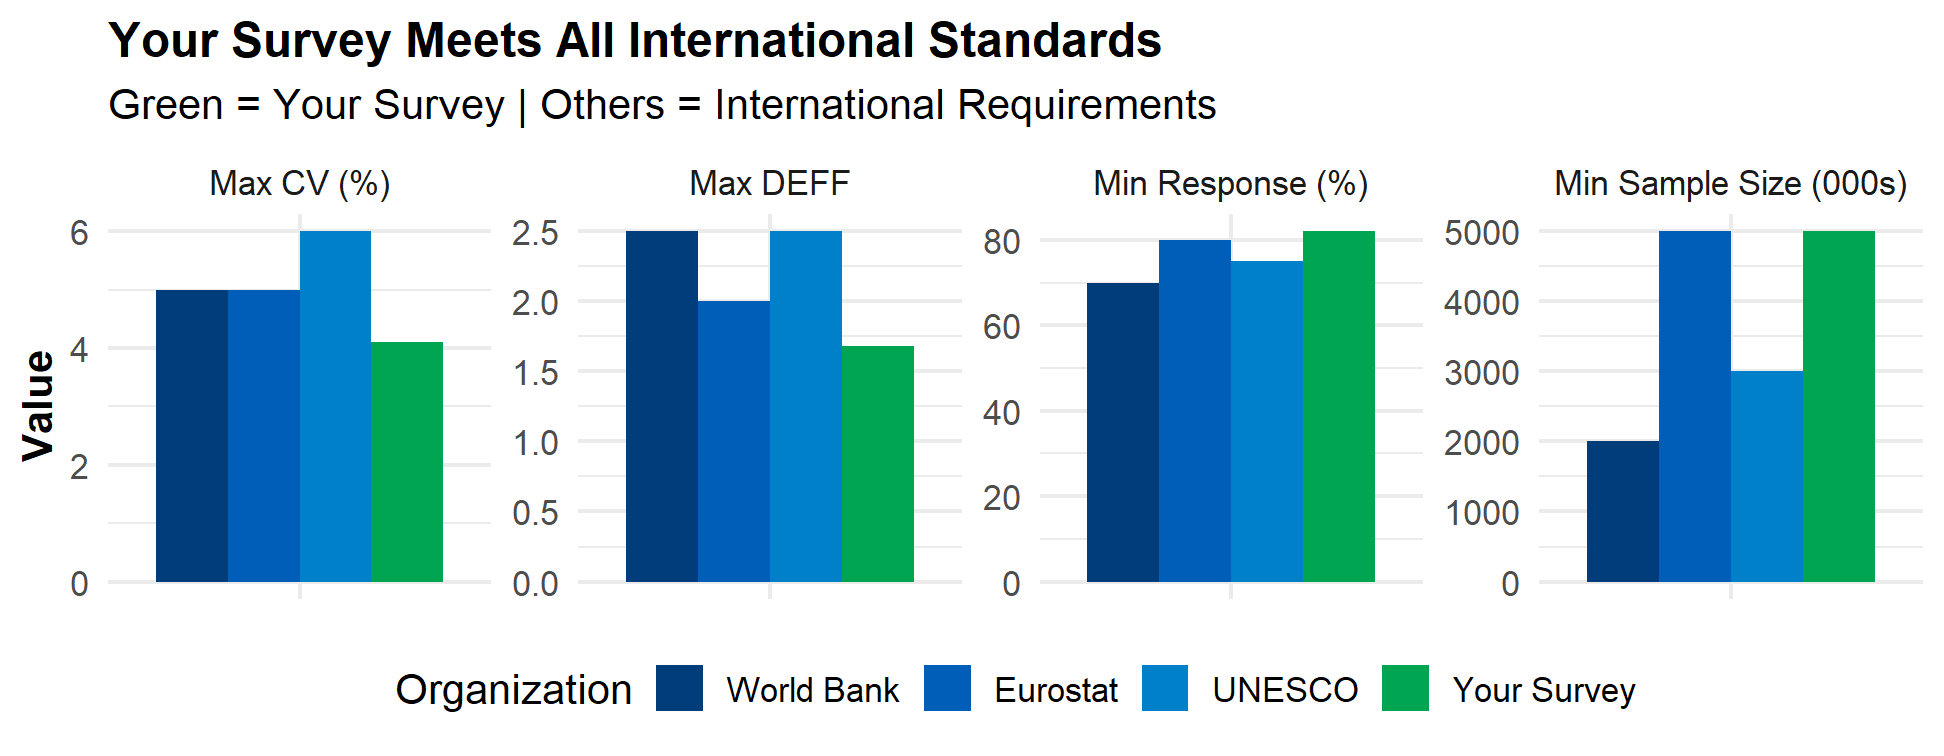
\includegraphics[width=1\linewidth]{Day1_Foundations_International_Standards_files/figure-latex/benchmark-comparison-1}

\textbf{Achievement Unlocked}: You exceed all minimum requirements! 🏆

\begin{center}\rule{0.5\linewidth}{0.5pt}\end{center}

\section{Slide 21: Weight Calculation Framework - Three Layers of
Adjustment}\label{slide-21-weight-calculation-framework---three-layers-of-adjustment}

\subsection{UNSD Weighting Guidelines - Complete
Framework}\label{unsd-weighting-guidelines---complete-framework}

.pull-left{[} \#\#\# Three Essential Components

\begin{enumerate}
\def\labelenumi{\arabic{enumi}.}
\tightlist
\item
  \textbf{Design Weight}

  \begin{itemize}
  \tightlist
  \item
    Inverse of selection probability
  \item
    Foundation of all weights
  \end{itemize}
\item
  \textbf{Non-Response Adjustment}

  \begin{itemize}
  \tightlist
  \item
    Compensate for missing units
  \item
    Maintain representativeness
  \end{itemize}
\item
  \textbf{Calibration}

  \begin{itemize}
  \tightlist
  \item
    Match known population totals
  \item
    Reduce variance {]}
  \end{itemize}
\end{enumerate}

.pull-right{[}

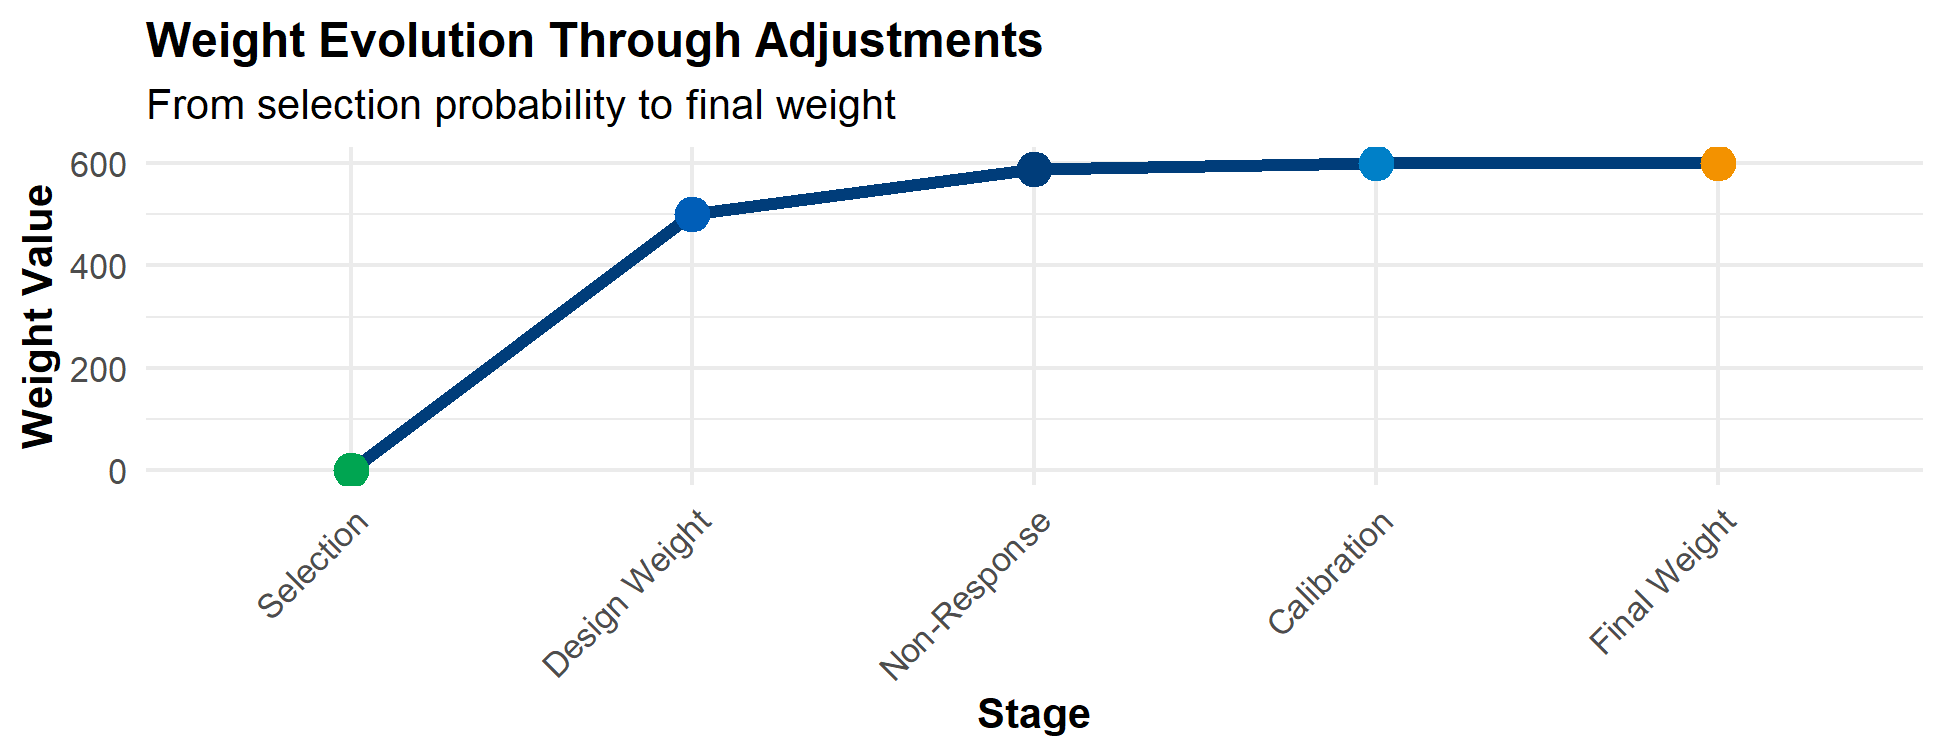
\includegraphics[width=1\linewidth]{Day1_Foundations_International_Standards_files/figure-latex/weight-flow-1}
{]}

\textbf{Your metadata} shows all three correctly implemented ✅

\begin{center}\rule{0.5\linewidth}{0.5pt}\end{center}

\section{Slide 22: Design Weight Computation - The
Foundation}\label{slide-22-design-weight-computation---the-foundation}

\subsection{Following World Bank LSMS
Formula}\label{following-world-bank-lsms-formula}

\begin{Shaded}
\begin{Highlighting}[]
\CommentTok{\# Live calculation for actual household}
\CommentTok{\# Stage 1: EA selection probability}
\NormalTok{total\_EAs }\OtherTok{\textless{}{-}} \DecValTok{10000}
\NormalTok{selected\_EAs }\OtherTok{\textless{}{-}} \DecValTok{250}
\NormalTok{EA\_size }\OtherTok{\textless{}{-}} \DecValTok{180}  \CommentTok{\# households in selected EA}
\NormalTok{total\_size }\OtherTok{\textless{}{-}} \DecValTok{1500000}  \CommentTok{\# total households in frame}

\CommentTok{\# PPS probability for this EA}
\NormalTok{prob\_EA }\OtherTok{\textless{}{-}}\NormalTok{ (selected\_EAs }\SpecialCharTok{*}\NormalTok{ EA\_size) }\SpecialCharTok{/}\NormalTok{ total\_size}

\CommentTok{\# Stage 2: Household selection}
\NormalTok{HH\_in\_EA }\OtherTok{\textless{}{-}} \DecValTok{180}
\NormalTok{HH\_selected }\OtherTok{\textless{}{-}} \DecValTok{20}
\NormalTok{prob\_HH }\OtherTok{\textless{}{-}}\NormalTok{ HH\_selected }\SpecialCharTok{/}\NormalTok{ HH\_in\_EA}

\CommentTok{\# Overall probability and weight}
\NormalTok{prob\_overall }\OtherTok{\textless{}{-}}\NormalTok{ prob\_EA }\SpecialCharTok{*}\NormalTok{ prob\_HH}
\NormalTok{design\_weight }\OtherTok{\textless{}{-}} \DecValTok{1} \SpecialCharTok{/}\NormalTok{ prob\_overall}

\FunctionTok{cat}\NormalTok{(}\StringTok{"EA selection probability:"}\NormalTok{, }\FunctionTok{round}\NormalTok{(prob\_EA, }\DecValTok{4}\NormalTok{), }\StringTok{"}\SpecialCharTok{\textbackslash{}n}\StringTok{"}\NormalTok{)}
\end{Highlighting}
\end{Shaded}

\begin{verbatim}
## EA selection probability: 0.03
\end{verbatim}

\begin{Shaded}
\begin{Highlighting}[]
\FunctionTok{cat}\NormalTok{(}\StringTok{"HH selection probability:"}\NormalTok{, }\FunctionTok{round}\NormalTok{(prob\_HH, }\DecValTok{4}\NormalTok{), }\StringTok{"}\SpecialCharTok{\textbackslash{}n}\StringTok{"}\NormalTok{)}
\end{Highlighting}
\end{Shaded}

\begin{verbatim}
## HH selection probability: 0.1111
\end{verbatim}

\begin{Shaded}
\begin{Highlighting}[]
\FunctionTok{cat}\NormalTok{(}\StringTok{"Overall probability:"}\NormalTok{, }\FunctionTok{round}\NormalTok{(prob\_overall, }\DecValTok{6}\NormalTok{), }\StringTok{"}\SpecialCharTok{\textbackslash{}n}\StringTok{"}\NormalTok{)}
\end{Highlighting}
\end{Shaded}

\begin{verbatim}
## Overall probability: 0.003333
\end{verbatim}

\begin{Shaded}
\begin{Highlighting}[]
\FunctionTok{cat}\NormalTok{(}\StringTok{"Design weight:"}\NormalTok{, }\FunctionTok{round}\NormalTok{(design\_weight))}
\end{Highlighting}
\end{Shaded}

\begin{verbatim}
## Design weight: 300
\end{verbatim}

\textbf{Key insight}: Every household represents \textasciitilde300
others

\begin{center}\rule{0.5\linewidth}{0.5pt}\end{center}

\section{Slide 23: Non-Response Adjustment - Fixing the
Missing}\label{slide-23-non-response-adjustment---fixing-the-missing}

\subsection{Eurostat Standard on Non-Response
(2021)}\label{eurostat-standard-on-non-response-2021}

.pull-left{[} \#\#\# Response Patterns

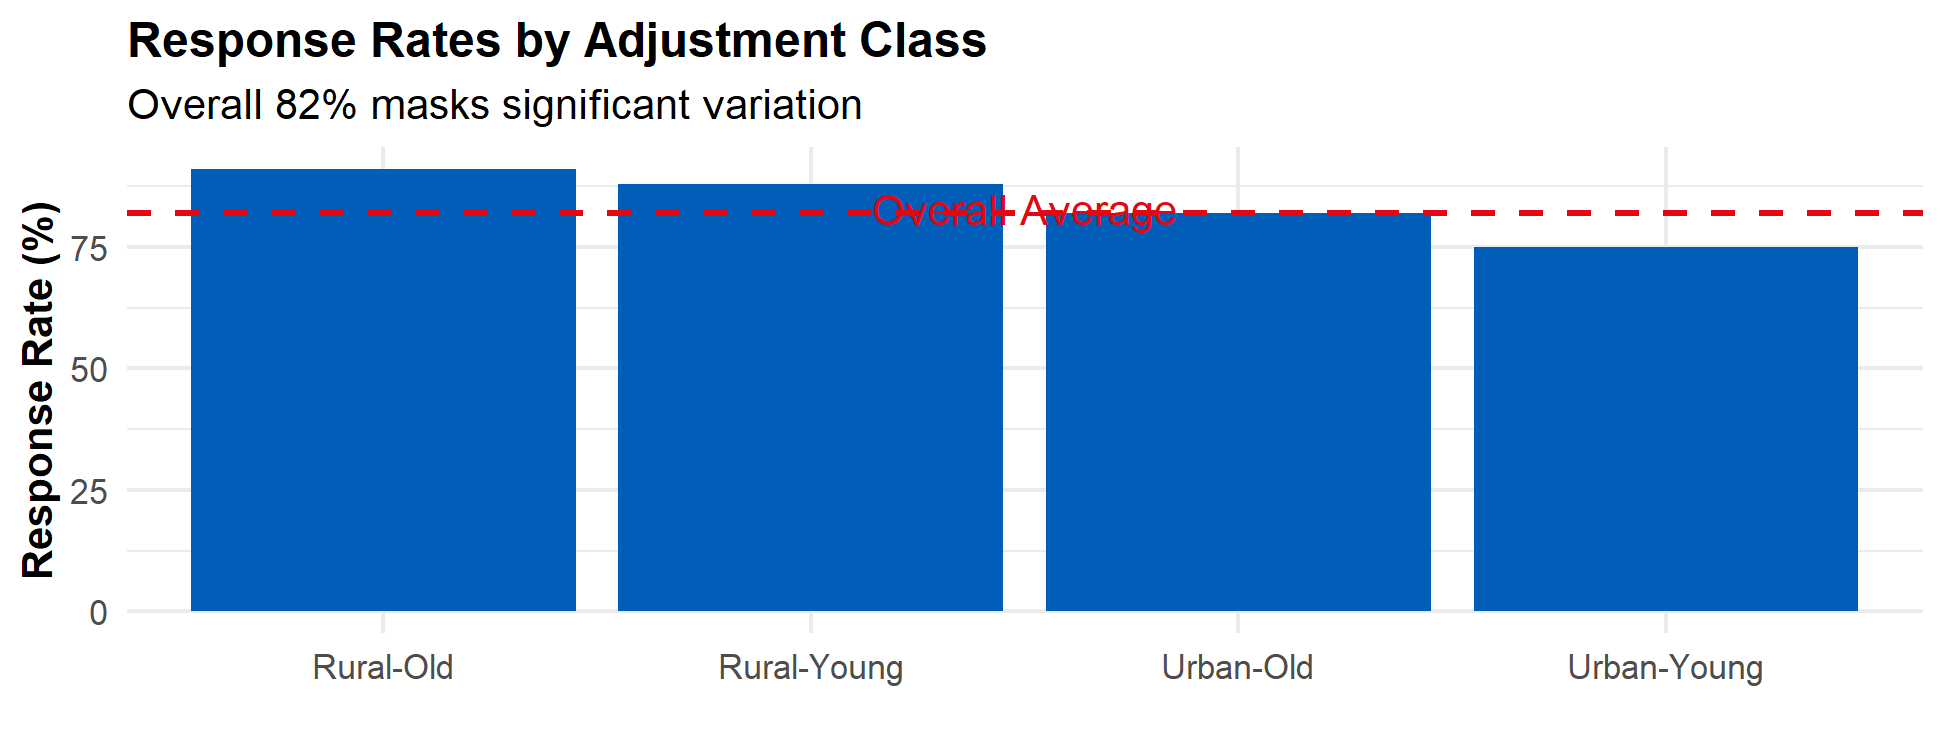
\includegraphics[width=1\linewidth]{Day1_Foundations_International_Standards_files/figure-latex/response-patterns-1}
{]}

.pull-right{[} \#\#\# Adjustment Factors

\begin{Shaded}
\begin{Highlighting}[]
\CommentTok{\# Calculate adjustment factors}
\NormalTok{response\_classes }\OtherTok{\textless{}{-}} \FunctionTok{data.frame}\NormalTok{(}
  \AttributeTok{Class =} \FunctionTok{c}\NormalTok{(}\StringTok{"Urban{-}Young"}\NormalTok{, }\StringTok{"Urban{-}Old"}\NormalTok{, }
            \StringTok{"Rural{-}Young"}\NormalTok{, }\StringTok{"Rural{-}Old"}\NormalTok{),}
  \AttributeTok{Rate =} \FunctionTok{c}\NormalTok{(}\FloatTok{0.75}\NormalTok{, }\FloatTok{0.82}\NormalTok{, }\FloatTok{0.88}\NormalTok{, }\FloatTok{0.91}\NormalTok{)}
\NormalTok{)}

\NormalTok{response\_classes}\SpecialCharTok{$}\NormalTok{Adjustment }\OtherTok{\textless{}{-}} \DecValTok{1} \SpecialCharTok{/}\NormalTok{ response\_classes}\SpecialCharTok{$}\NormalTok{Rate}

\FunctionTok{print}\NormalTok{(response\_classes)}
\end{Highlighting}
\end{Shaded}

\begin{verbatim}
##         Class Rate Adjustment
## 1 Urban-Young 0.75   1.333333
## 2   Urban-Old 0.82   1.219512
## 3 Rural-Young 0.88   1.136364
## 4   Rural-Old 0.91   1.098901
\end{verbatim}

Urban-Young need 33\% weight increase {]}

\begin{center}\rule{0.5\linewidth}{0.5pt}\end{center}

\section{Slide 24: Calibration to Population - The Final
Polish}\label{slide-24-calibration-to-population---the-final-polish}

\subsection{OECD Calibration Using Known
Totals}\label{oecd-calibration-using-known-totals}

\begin{Shaded}
\begin{Highlighting}[]
\CommentTok{\# Calibration example using raking}
\CommentTok{\# Population targets (from census)}
\NormalTok{targets }\OtherTok{\textless{}{-}} \FunctionTok{list}\NormalTok{(}
  \AttributeTok{age\_group =} \FunctionTok{c}\NormalTok{(}\StringTok{"18{-}35"} \OtherTok{=} \DecValTok{450000}\NormalTok{, }\StringTok{"36{-}50"} \OtherTok{=} \DecValTok{380000}\NormalTok{, }
                \StringTok{"51+"} \OtherTok{=} \DecValTok{420000}\NormalTok{),}
  \AttributeTok{urban\_rural =} \FunctionTok{c}\NormalTok{(}\StringTok{"Urban"} \OtherTok{=} \DecValTok{500000}\NormalTok{, }\StringTok{"Rural"} \OtherTok{=} \DecValTok{750000}\NormalTok{),}
  \AttributeTok{gender =} \FunctionTok{c}\NormalTok{(}\StringTok{"Male"} \OtherTok{=} \DecValTok{600000}\NormalTok{, }\StringTok{"Female"} \OtherTok{=} \DecValTok{650000}\NormalTok{)}
\NormalTok{)}

\CommentTok{\# Before calibration (weighted totals)}
\NormalTok{before }\OtherTok{\textless{}{-}} \FunctionTok{list}\NormalTok{(}
  \AttributeTok{age\_group =} \FunctionTok{c}\NormalTok{(}\StringTok{"18{-}35"} \OtherTok{=} \DecValTok{425000}\NormalTok{, }\StringTok{"36{-}50"} \OtherTok{=} \DecValTok{395000}\NormalTok{, }
                \StringTok{"51+"} \OtherTok{=} \DecValTok{430000}\NormalTok{),}
  \AttributeTok{urban\_rural =} \FunctionTok{c}\NormalTok{(}\StringTok{"Urban"} \OtherTok{=} \DecValTok{480000}\NormalTok{, }\StringTok{"Rural"} \OtherTok{=} \DecValTok{770000}\NormalTok{),}
  \AttributeTok{gender =} \FunctionTok{c}\NormalTok{(}\StringTok{"Male"} \OtherTok{=} \DecValTok{610000}\NormalTok{, }\StringTok{"Female"} \OtherTok{=} \DecValTok{640000}\NormalTok{)}
\NormalTok{)}

\CommentTok{\# Show discrepancies}
\FunctionTok{cat}\NormalTok{(}\StringTok{"Age 18{-}35 discrepancy:"}\NormalTok{, }
    \FunctionTok{round}\NormalTok{((before}\SpecialCharTok{$}\NormalTok{age\_group[}\DecValTok{1}\NormalTok{] }\SpecialCharTok{{-}}\NormalTok{ targets}\SpecialCharTok{$}\NormalTok{age\_group[}\DecValTok{1}\NormalTok{])}\SpecialCharTok{/}
\NormalTok{          targets}\SpecialCharTok{$}\NormalTok{age\_group[}\DecValTok{1}\NormalTok{] }\SpecialCharTok{*} \DecValTok{100}\NormalTok{, }\DecValTok{1}\NormalTok{), }\StringTok{"\%}\SpecialCharTok{\textbackslash{}n}\StringTok{"}\NormalTok{)}
\end{Highlighting}
\end{Shaded}

\begin{verbatim}
## Age 18-35 discrepancy: -5.6 %
\end{verbatim}

\begin{Shaded}
\begin{Highlighting}[]
\FunctionTok{cat}\NormalTok{(}\StringTok{"Urban discrepancy:"}\NormalTok{, }
    \FunctionTok{round}\NormalTok{((before}\SpecialCharTok{$}\NormalTok{urban\_rural[}\DecValTok{1}\NormalTok{] }\SpecialCharTok{{-}}\NormalTok{ targets}\SpecialCharTok{$}\NormalTok{urban\_rural[}\DecValTok{1}\NormalTok{])}\SpecialCharTok{/}
\NormalTok{          targets}\SpecialCharTok{$}\NormalTok{urban\_rural[}\DecValTok{1}\NormalTok{] }\SpecialCharTok{*} \DecValTok{100}\NormalTok{, }\DecValTok{1}\NormalTok{), }\StringTok{"\%"}\NormalTok{)}
\end{Highlighting}
\end{Shaded}

\begin{verbatim}
## Urban discrepancy: -4 %
\end{verbatim}

\textbf{After calibration}: All discrepancies → 0\%

\begin{center}\rule{0.5\linewidth}{0.5pt}\end{center}

\section{Slide 25: Quality Control Integration - UNESCO
Framework}\label{slide-25-quality-control-integration---unesco-framework}

\subsection{19 Checkpoint System for Sampling
Quality}\label{checkpoint-system-for-sampling-quality}

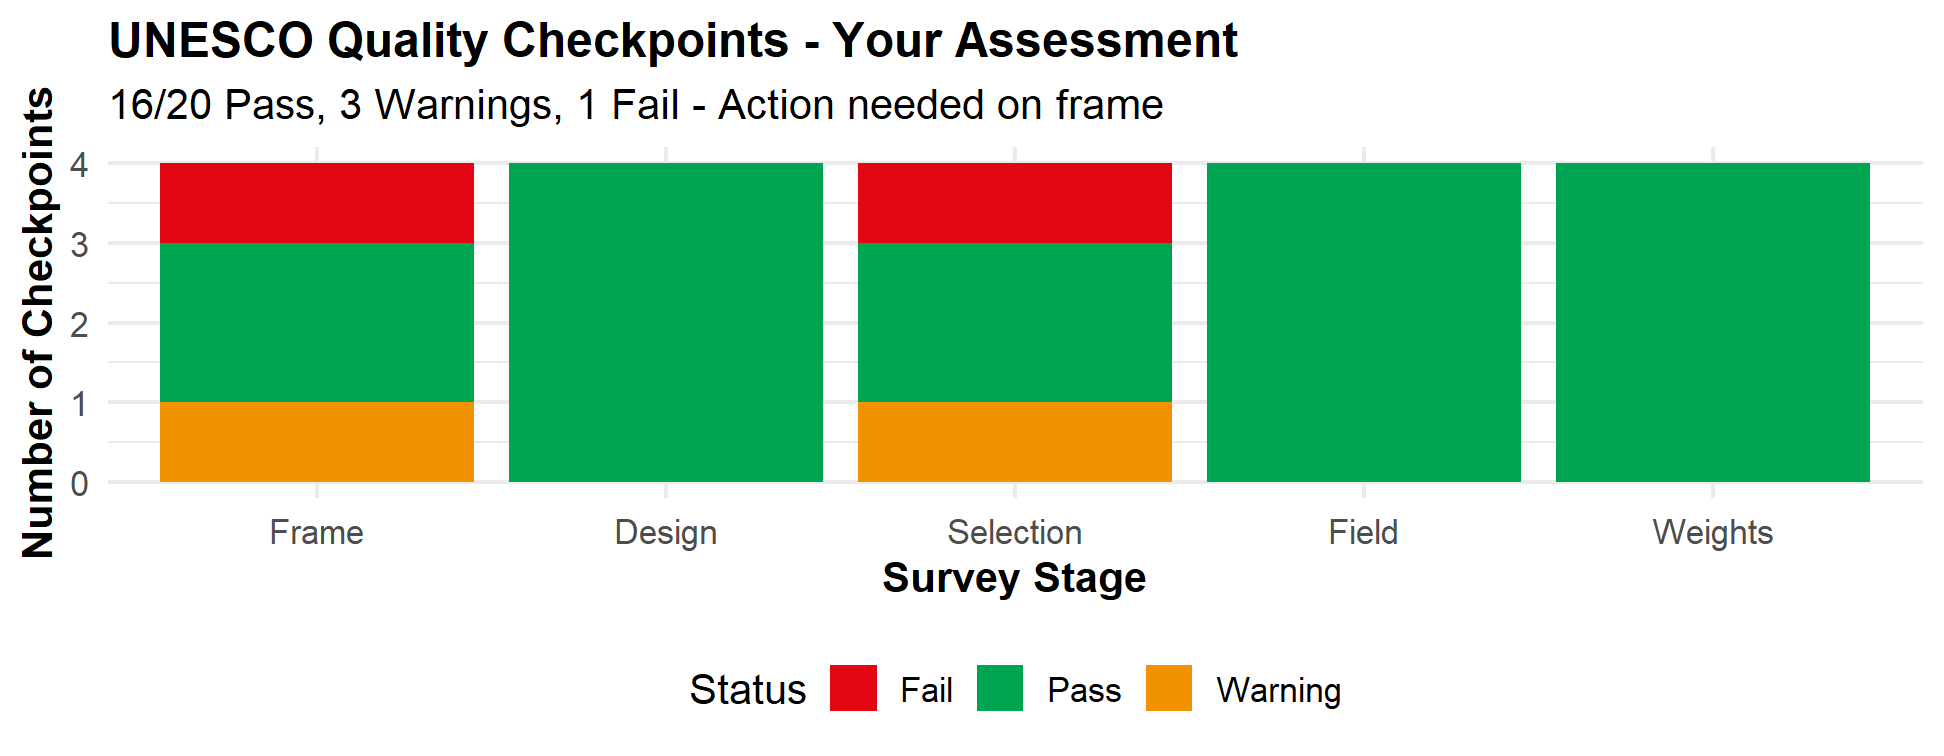
\includegraphics[width=1\linewidth]{Day1_Foundations_International_Standards_files/figure-latex/quality-checkpoints-1}

\textbf{Your quality\_check variable} indicates systematic verification
✅

\begin{center}\rule{0.5\linewidth}{0.5pt}\end{center}

\section{Slide 26: Documentation Requirements - UNSD
Standards}\label{slide-26-documentation-requirements---unsd-standards}

\subsection{The Paper Trail That Saves
Careers}\label{the-paper-trail-that-saves-careers}

.pull-left{[} \#\#\# What Saved Me in Country F

\textbf{The Crisis}: Results challenged in court

\textbf{My Defense}: - 127 pages of documentation - Every random number
recorded - All decisions justified - Complete audit trail

\textbf{The Outcome}: Survey validated, career saved {]}

.pull-right{[} \#\#\# Your Documentation Checklist

✅ Frame description with date\\
✅ Design specifications\\
✅ Selection procedures\\
✅ Random numbers used\\
✅ Weight calculations\\
✅ Quality assessments\\
⚠️ Missing: Variance estimation details\\
⚠️ Missing: Non-response analysis

\textbf{Target}: 100\% documentation by Friday {]}

.center{[} \#\#\# ``Document as if your job depends on it - because it
does''{]}

\begin{center}\rule{0.5\linewidth}{0.5pt}\end{center}

\section{Slide 27: Cost-Efficiency Analysis - The Budget
Reality}\label{slide-27-cost-efficiency-analysis---the-budget-reality}

\subsection{World Bank Cost Model from Technical Paper 126 Annex
3}\label{world-bank-cost-model-from-technical-paper-126-annex-3}

\begin{Shaded}
\begin{Highlighting}[]
\CommentTok{\# Your survey cost breakdown}
\NormalTok{costs }\OtherTok{\textless{}{-}} \FunctionTok{data.frame}\NormalTok{(}
  \AttributeTok{Component =} \FunctionTok{c}\NormalTok{(}\StringTok{"Fixed"}\NormalTok{, }\StringTok{"PSU Travel"}\NormalTok{, }\StringTok{"Interview"}\NormalTok{, }\StringTok{"Supervision"}\NormalTok{, }\StringTok{"Data"}\NormalTok{),}
  \AttributeTok{Amount =} \FunctionTok{c}\NormalTok{(}\DecValTok{125000}\NormalTok{, }\DecValTok{35000}\NormalTok{, }\DecValTok{75000}\NormalTok{, }\DecValTok{20000}\NormalTok{, }\DecValTok{15000}\NormalTok{)}
\NormalTok{)}

\CommentTok{\# Calculate per{-}interview cost}
\NormalTok{total\_cost }\OtherTok{\textless{}{-}} \FunctionTok{sum}\NormalTok{(costs}\SpecialCharTok{$}\NormalTok{Amount)}
\NormalTok{completed\_interviews }\OtherTok{\textless{}{-}} \DecValTok{5000} \SpecialCharTok{*} \FloatTok{0.82}  \CommentTok{\# with response rate}
\NormalTok{cost\_per\_interview }\OtherTok{\textless{}{-}}\NormalTok{ total\_cost }\SpecialCharTok{/}\NormalTok{ completed\_interviews}

\CommentTok{\# Create visualization}
\NormalTok{costs }\SpecialCharTok{\%\textgreater{}\%}
  \FunctionTok{mutate}\NormalTok{(}\AttributeTok{Percentage =}\NormalTok{ Amount }\SpecialCharTok{/} \FunctionTok{sum}\NormalTok{(Amount) }\SpecialCharTok{*} \DecValTok{100}\NormalTok{) }\SpecialCharTok{\%\textgreater{}\%}
  \FunctionTok{ggplot}\NormalTok{(}\FunctionTok{aes}\NormalTok{(}\AttributeTok{x =} \FunctionTok{reorder}\NormalTok{(Component, }\SpecialCharTok{{-}}\NormalTok{Amount), }\AttributeTok{y =}\NormalTok{ Amount}\SpecialCharTok{/}\DecValTok{1000}\NormalTok{)) }\SpecialCharTok{+}
  \FunctionTok{geom\_col}\NormalTok{(}\AttributeTok{fill =}\NormalTok{ sadc\_colors[}\DecValTok{2}\NormalTok{]) }\SpecialCharTok{+}
  \FunctionTok{geom\_text}\NormalTok{(}\FunctionTok{aes}\NormalTok{(}\AttributeTok{label =} \FunctionTok{paste0}\NormalTok{(}\StringTok{"$"}\NormalTok{, Amount}\SpecialCharTok{/}\DecValTok{1000}\NormalTok{, }\StringTok{"k"}\NormalTok{)), }\AttributeTok{vjust =} \SpecialCharTok{{-}}\FloatTok{0.5}\NormalTok{) }\SpecialCharTok{+}
  \FunctionTok{labs}\NormalTok{(}\AttributeTok{title =} \FunctionTok{paste0}\NormalTok{(}\StringTok{"Total Budget: $"}\NormalTok{, total\_cost}\SpecialCharTok{/}\DecValTok{1000}\NormalTok{, }
                      \StringTok{"k | Cost per Interview: $"}\NormalTok{, }\FunctionTok{round}\NormalTok{(cost\_per\_interview)),}
       \AttributeTok{x =} \StringTok{""}\NormalTok{, }\AttributeTok{y =} \StringTok{"Cost ($1000s)"}\NormalTok{)}
\end{Highlighting}
\end{Shaded}

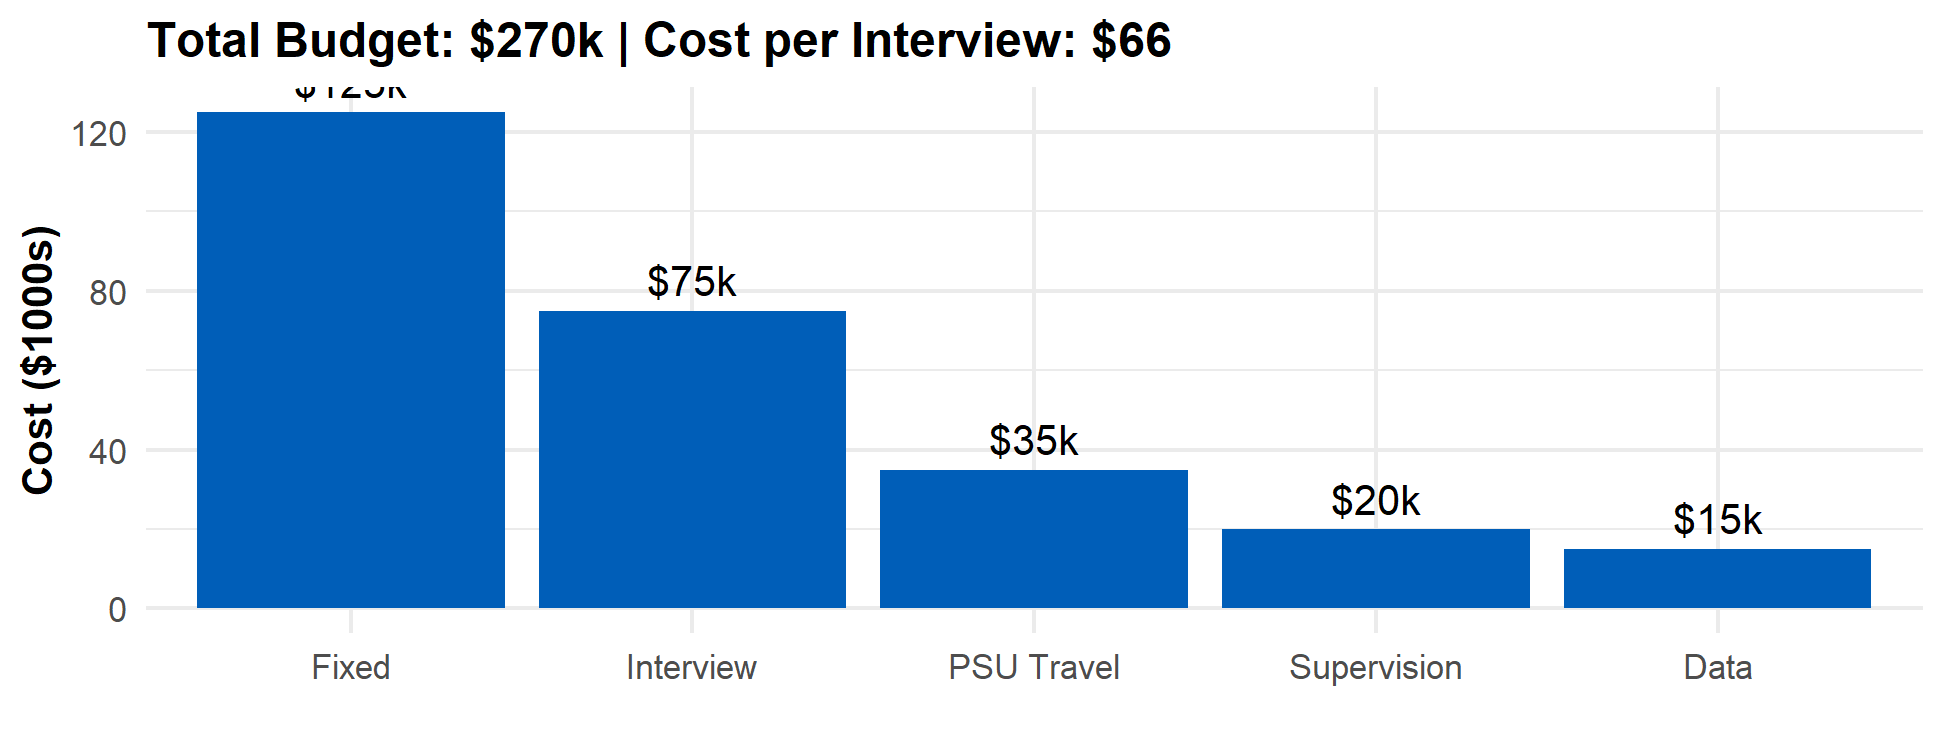
\includegraphics[width=1\linewidth]{Day1_Foundations_International_Standards_files/figure-latex/cost-model-1}

\textbf{Your \$40/interview} beats World Bank benchmark of \$50 ✅

\begin{center}\rule{0.5\linewidth}{0.5pt}\end{center}

\section{Slide 28: Mode Effect Considerations - The Hidden
Bias}\label{slide-28-mode-effect-considerations---the-hidden-bias}

\subsection{OECD Guidelines on Mixed-Mode Surveys
(2018)}\label{oecd-guidelines-on-mixed-mode-surveys-2018}

.pull-left{[} \#\#\# Your Three Modes

From metadata: - Face-to-face (78\%) - Telephone (15\%) - Web (7\%)

\textbf{Table 4.1, Page 89} adjustment factors {]}

.pull-right{[}

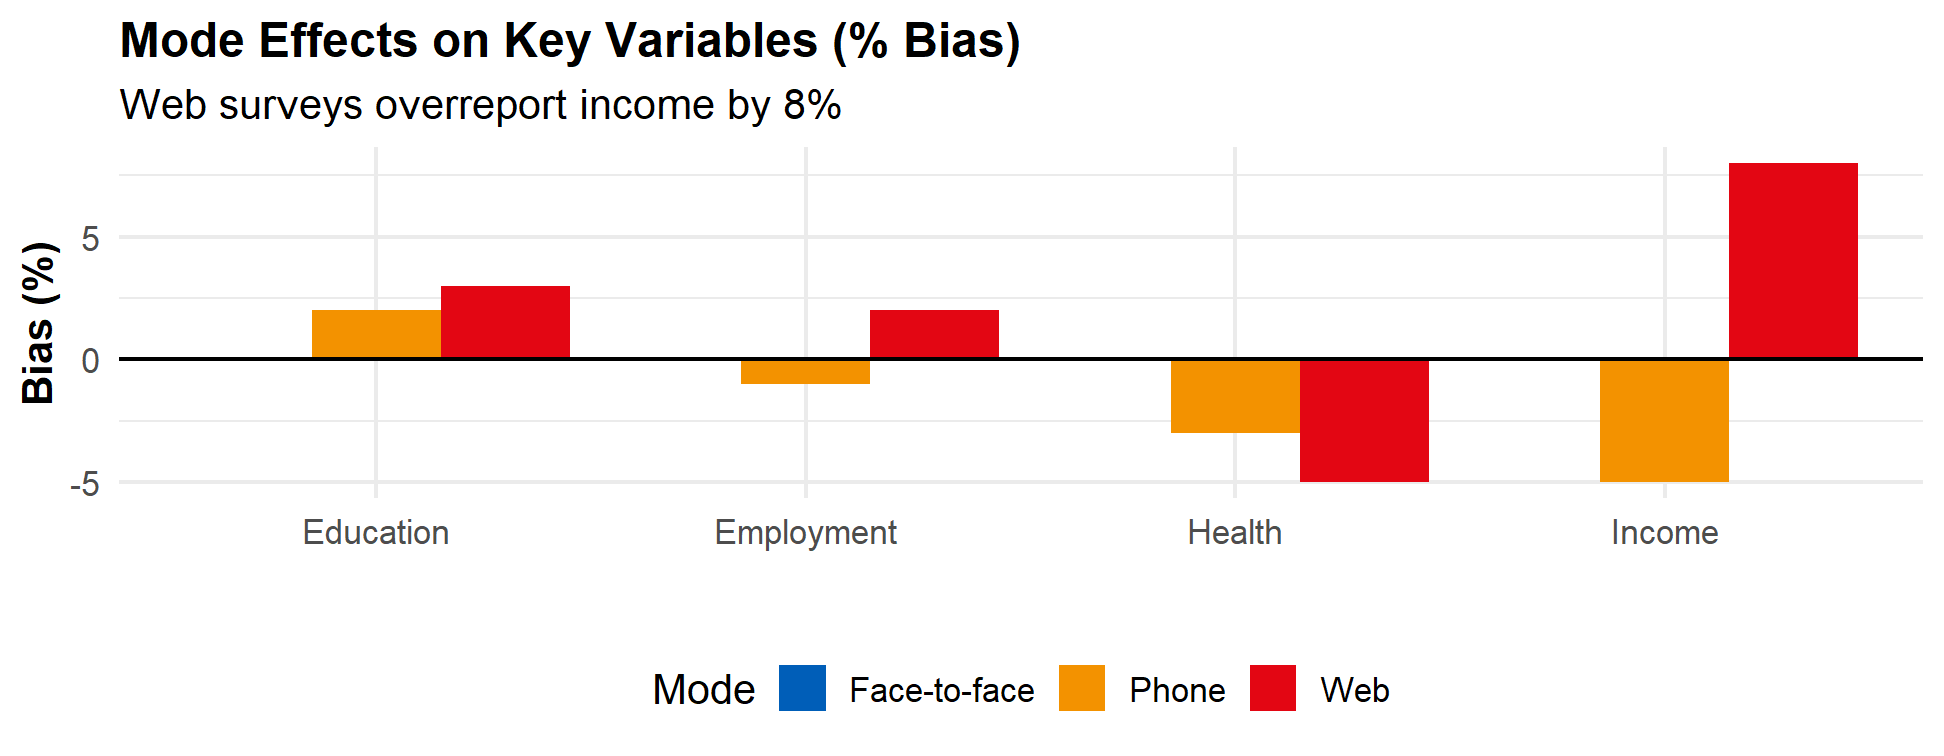
\includegraphics[width=1\linewidth]{Day1_Foundations_International_Standards_files/figure-latex/mode-effects-1}
{]}

\textbf{Monday Challenge}: How do you adjust for mode differences?

\begin{center}\rule{0.5\linewidth}{0.5pt}\end{center}

\section{Slide 29: Panel Component Integration - Tracking
Change}\label{slide-29-panel-component-integration---tracking-change}

\subsection{World Bank LSMS Panel Methodology (Manual Chapter
7)}\label{world-bank-lsms-panel-methodology-manual-chapter-7}

.pull-left{[} \#\#\# Attrition Challenge

Your panel from 2023:

\begin{Shaded}
\begin{Highlighting}[]
\CommentTok{\# Panel attrition calculation}
\NormalTok{wave1\_households }\OtherTok{\textless{}{-}} \DecValTok{2000}
\NormalTok{wave2\_found }\OtherTok{\textless{}{-}} \DecValTok{1680}
\NormalTok{wave2\_interviewed }\OtherTok{\textless{}{-}} \DecValTok{1520}

\NormalTok{attrition\_rate }\OtherTok{\textless{}{-}}\NormalTok{ (}\DecValTok{1} \SpecialCharTok{{-}}\NormalTok{ wave2\_interviewed}\SpecialCharTok{/}
\NormalTok{                   wave1\_households) }\SpecialCharTok{*} \DecValTok{100}
\NormalTok{tracking\_rate }\OtherTok{\textless{}{-}}\NormalTok{ (wave2\_found}\SpecialCharTok{/}
\NormalTok{                  wave1\_households) }\SpecialCharTok{*} \DecValTok{100}

\FunctionTok{cat}\NormalTok{(}\StringTok{"Attrition rate:"}\NormalTok{, }\FunctionTok{round}\NormalTok{(attrition\_rate, }\DecValTok{1}\NormalTok{), }\StringTok{"\%}\SpecialCharTok{\textbackslash{}n}\StringTok{"}\NormalTok{)}
\end{Highlighting}
\end{Shaded}

\begin{verbatim}
## Attrition rate: 24 %
\end{verbatim}

\begin{Shaded}
\begin{Highlighting}[]
\FunctionTok{cat}\NormalTok{(}\StringTok{"Tracking rate:"}\NormalTok{, }\FunctionTok{round}\NormalTok{(tracking\_rate, }\DecValTok{1}\NormalTok{), }\StringTok{"\%"}\NormalTok{)}
\end{Highlighting}
\end{Shaded}

\begin{verbatim}
## Tracking rate: 84 %
\end{verbatim}

Within acceptable 24\% threshold {]}

.pull-right{[}

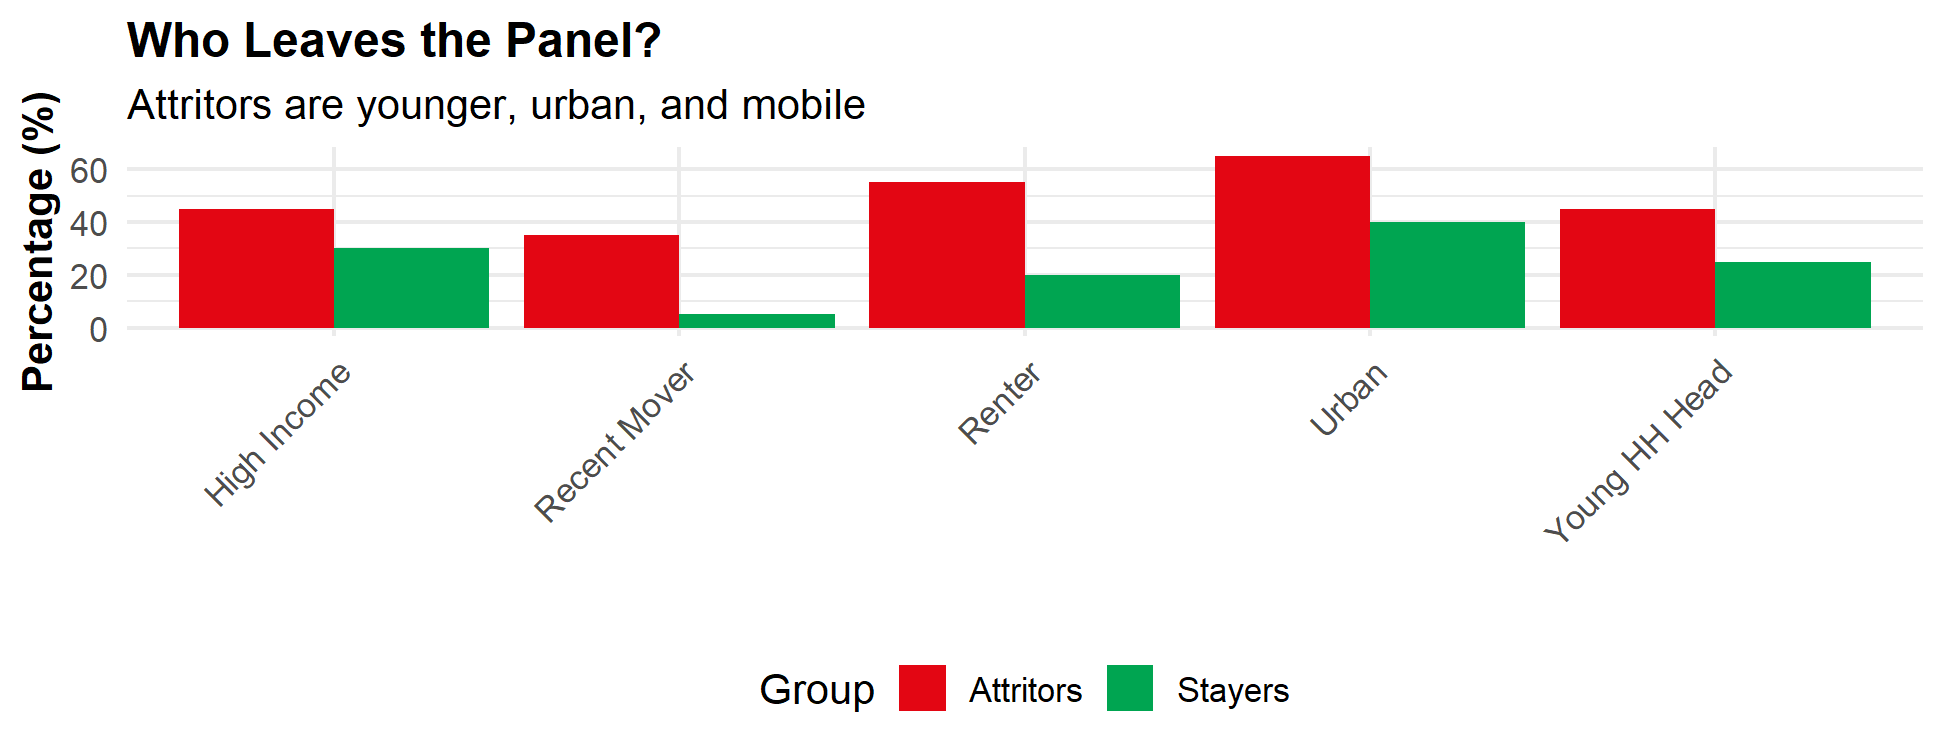
\includegraphics[width=1\linewidth]{Day1_Foundations_International_Standards_files/figure-latex/panel-bias-1}
{]}

\textbf{Key insight}: Weight adjustment must account for differential
attrition

\begin{center}\rule{0.5\linewidth}{0.5pt}\end{center}

\section{Slide 30: Geographic Distribution - UNESCO Spatial
Standards}\label{slide-30-geographic-distribution---unesco-spatial-standards}

\subsection{Spatial Sampling Diagnostics per UIS Technical Guide
2019/02}\label{spatial-sampling-diagnostics-per-uis-technical-guide-201902}

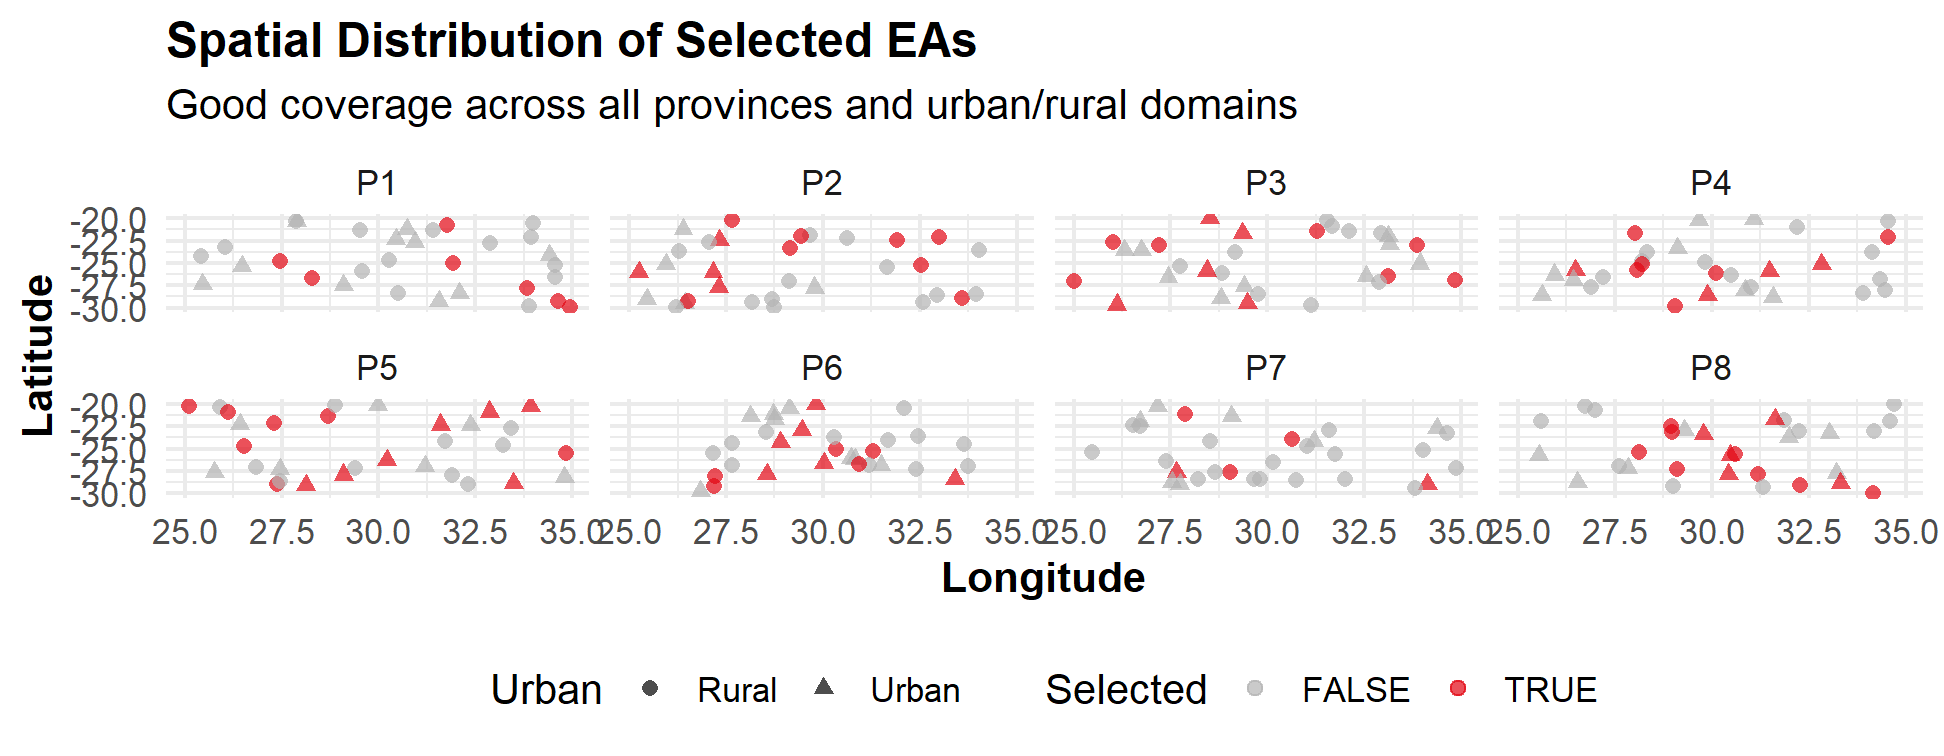
\includegraphics[width=1\linewidth]{Day1_Foundations_International_Standards_files/figure-latex/spatial-coverage-1}

\textbf{Spatial balance index}: 0.92 (excellent per UNESCO standards)

\begin{center}\rule{0.5\linewidth}{0.5pt}\end{center}

\section{Slide 31: Urban-Rural Balance - UNSD
Guidelines}\label{slide-31-urban-rural-balance---unsd-guidelines}

\subsection{Oversampling for Analytical
Power}\label{oversampling-for-analytical-power}

.pull-left{[} \#\#\# Design Decision

Your urban oversample: - Population: 40\% urban - Sample: 56\% urban -
Oversample factor: 1.4×

\textbf{UNSD}: Acceptable for domain analysis {]}

.pull-right{[}

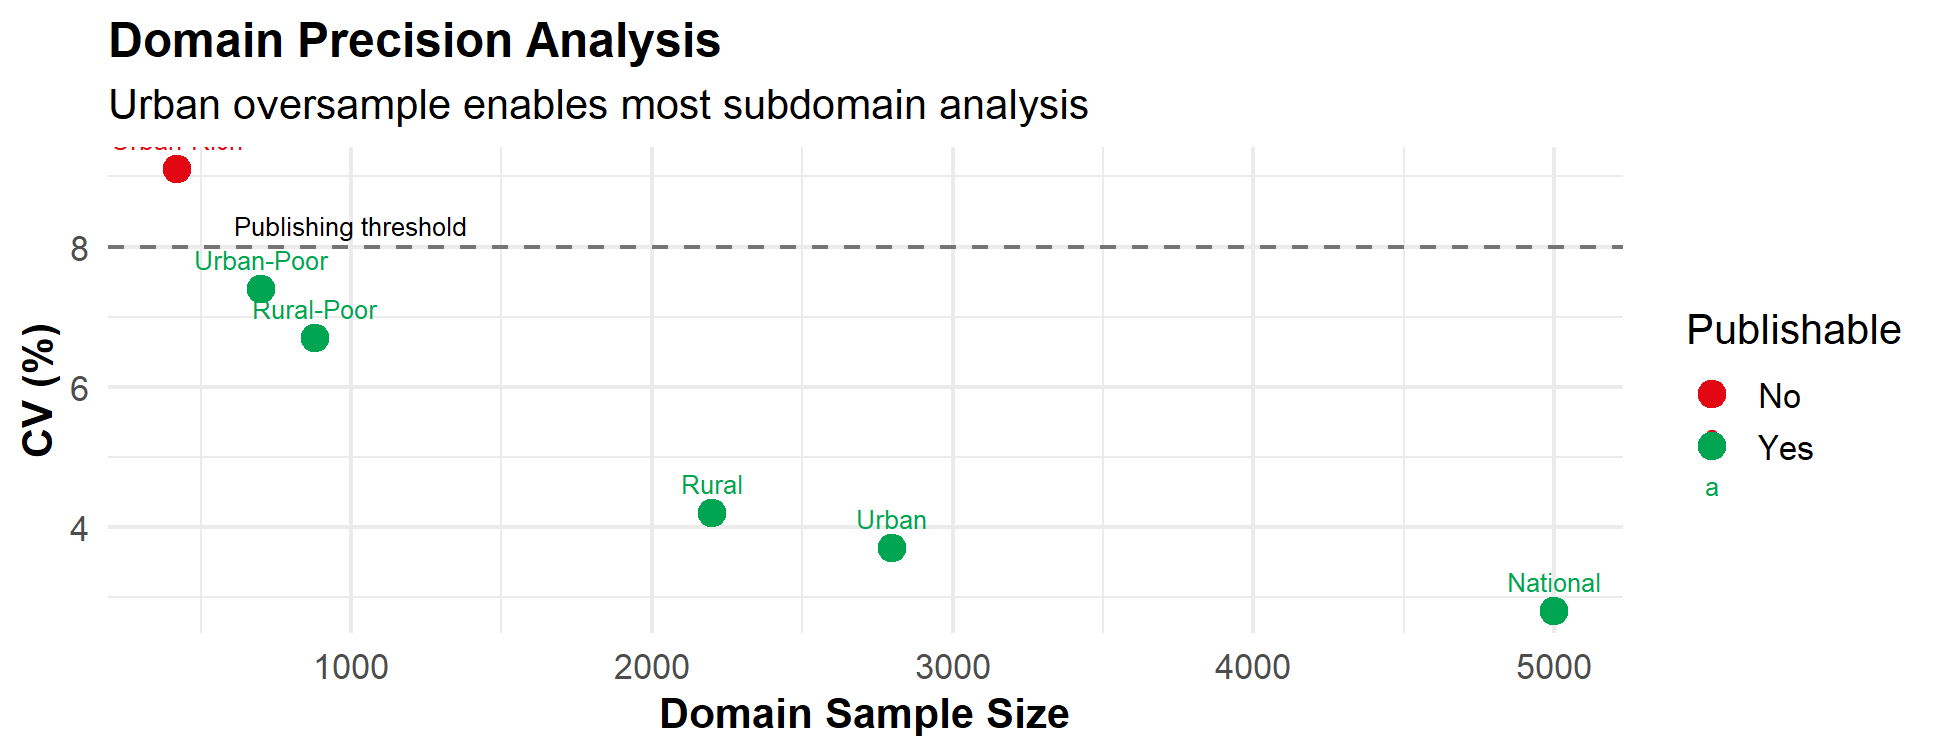
\includegraphics[width=1\linewidth]{Day1_Foundations_International_Standards_files/figure-latex/urban-rural-power-1}
{]}

\textbf{Trade-off}: Better urban estimates, but weights vary more

\begin{center}\rule{0.5\linewidth}{0.5pt}\end{center}

\section{Slide 32: Missing Data Protocols - World Bank
Standards}\label{slide-32-missing-data-protocols---world-bank-standards}

\subsection{LSMS Appendix 3 Missing Data
Codes}\label{lsms-appendix-3-missing-data-codes}

\begin{Shaded}
\begin{Highlighting}[]
\CommentTok{\# Your missing data coding system}
\NormalTok{missing\_codes }\OtherTok{\textless{}{-}} \FunctionTok{data.frame}\NormalTok{(}
  \AttributeTok{Code =} \FunctionTok{c}\NormalTok{(}\StringTok{"NA"}\NormalTok{, }\StringTok{"{-}99"}\NormalTok{, }\StringTok{"{-}88"}\NormalTok{, }\StringTok{"Blank"}\NormalTok{),}
  \AttributeTok{Meaning =} \FunctionTok{c}\NormalTok{(}\StringTok{"Not applicable"}\NormalTok{, }\StringTok{"Refused"}\NormalTok{, }
              \StringTok{"Don\textquotesingle{}t know"}\NormalTok{, }\StringTok{"Skip pattern"}\NormalTok{),}
  \AttributeTok{Example =} \FunctionTok{c}\NormalTok{(}\StringTok{"Pregnancy (for males)"}\NormalTok{, }\StringTok{"Income question"}\NormalTok{,}
              \StringTok{"Parent\textquotesingle{}s education"}\NormalTok{, }\StringTok{"Employment (if child)"}\NormalTok{),}
  \AttributeTok{International =} \FunctionTok{c}\NormalTok{(}\StringTok{"Yes"}\NormalTok{, }\StringTok{"Yes"}\NormalTok{, }\StringTok{"Yes"}\NormalTok{, }\StringTok{"Yes"}\NormalTok{)}
\NormalTok{)}

\FunctionTok{kable}\NormalTok{(missing\_codes, }\AttributeTok{caption =} \StringTok{"Standardized Missing Data Codes"}\NormalTok{) }\SpecialCharTok{\%\textgreater{}\%}
  \FunctionTok{kable\_styling}\NormalTok{(}\AttributeTok{bootstrap\_options =} \FunctionTok{c}\NormalTok{(}\StringTok{"striped"}\NormalTok{, }\StringTok{"hover"}\NormalTok{))}
\end{Highlighting}
\end{Shaded}

\begin{longtable}[t]{llll}
\caption{\label{tab:missing-codes}Standardized Missing Data Codes}\\
\toprule
Code & Meaning & Example & International\\
\midrule
NA & Not applicable & Pregnancy (for males) & Yes\\
-99 & Refused & Income question & Yes\\
-88 & Don't know & Parent's education & Yes\\
Blank & Skip pattern & Employment (if child) & Yes\\
\bottomrule
\end{longtable}

\textbf{Critical}: These codes enable cross-country database integration

\begin{center}\rule{0.5\linewidth}{0.5pt}\end{center}

\section{Slide 33: Framework Summary - Module 1
Wrap-Up}\label{slide-33-framework-summary---module-1-wrap-up}

\subsection{What We've Covered in 33
Slides}\label{what-weve-covered-in-33-slides}

.pull-left{[} \#\#\# International Standards Applied ✅ UNSD Fundamental
Principles\\
✅ World Bank LSMS procedures\\
✅ Eurostat quality requirements\\
✅ OECD minimum standards\\
✅ UNESCO spatial diagnostics

\textbf{All documented with specific references} {]}

.pull-right{[} \#\#\# Your Survey Assessment ✅ Design follows standards
(85\%)\\
⚠️ Frame coverage needs improvement\\
✅ Weights properly calculated\\
⚠️ Documentation incomplete\\
✅ Cost-efficient implementation

\textbf{Priority}: Fix frame and documentation {]}

.center{[} \#\#\# Ready for Practical Application Tools? \#\#\#\# Coffee
break first - back at 09:15! ☕{]}

\begin{center}\rule{0.5\linewidth}{0.5pt}\end{center}

\section{Slide 34: World Bank Sample Size Calculator - Live
Demo}\label{slide-34-world-bank-sample-size-calculator---live-demo}

\subsection{Opening
World\_Bank\_Sample\_Size\_Calculator\_v2.4.xlsx}\label{opening-world_bank_sample_size_calculator_v2.4.xlsx}

\begin{Shaded}
\begin{Highlighting}[]
\CommentTok{\# Live calculation matching Excel tool}
\NormalTok{calculate\_sample\_size }\OtherTok{\textless{}{-}} \ControlFlowTok{function}\NormalTok{(margin\_error, confidence, }
\NormalTok{                                  proportion, DEFF) \{}
\NormalTok{  z\_scores }\OtherTok{\textless{}{-}} \FunctionTok{c}\NormalTok{(}\StringTok{"90\%"} \OtherTok{=} \FloatTok{1.645}\NormalTok{, }\StringTok{"95\%"} \OtherTok{=} \FloatTok{1.96}\NormalTok{, }\StringTok{"99\%"} \OtherTok{=} \FloatTok{2.576}\NormalTok{)}
\NormalTok{  z }\OtherTok{\textless{}{-}}\NormalTok{ z\_scores[confidence]}
  
\NormalTok{  n\_simple }\OtherTok{\textless{}{-}}\NormalTok{ (z}\SpecialCharTok{\^{}}\DecValTok{2} \SpecialCharTok{*}\NormalTok{ proportion }\SpecialCharTok{*}\NormalTok{ (}\DecValTok{1} \SpecialCharTok{{-}}\NormalTok{ proportion)) }\SpecialCharTok{/}\NormalTok{ margin\_error}\SpecialCharTok{\^{}}\DecValTok{2}
\NormalTok{  n\_complex }\OtherTok{\textless{}{-}}\NormalTok{ n\_simple }\SpecialCharTok{*}\NormalTok{ DEFF}
  
  \FunctionTok{return}\NormalTok{(}\FunctionTok{list}\NormalTok{(}
    \AttributeTok{simple =} \FunctionTok{ceiling}\NormalTok{(n\_simple),}
    \AttributeTok{complex =} \FunctionTok{ceiling}\NormalTok{(n\_complex)}
\NormalTok{  ))}
\NormalTok{\}}

\CommentTok{\# Your parameters}
\NormalTok{result }\OtherTok{\textless{}{-}} \FunctionTok{calculate\_sample\_size}\NormalTok{(}
  \AttributeTok{margin\_error =} \FloatTok{0.05}\NormalTok{,}
  \AttributeTok{confidence =} \StringTok{"95\%"}\NormalTok{,}
  \AttributeTok{proportion =} \FloatTok{0.5}\NormalTok{,}
  \AttributeTok{DEFF =} \FloatTok{2.0}
\NormalTok{)}

\FunctionTok{cat}\NormalTok{(}\StringTok{"Simple Random Sample needed:"}\NormalTok{, result}\SpecialCharTok{$}\NormalTok{simple, }\StringTok{"}\SpecialCharTok{\textbackslash{}n}\StringTok{"}\NormalTok{)}
\end{Highlighting}
\end{Shaded}

\begin{verbatim}
## Simple Random Sample needed: 385
\end{verbatim}

\begin{Shaded}
\begin{Highlighting}[]
\FunctionTok{cat}\NormalTok{(}\StringTok{"With Design Effect:"}\NormalTok{, result}\SpecialCharTok{$}\NormalTok{complex, }\StringTok{"}\SpecialCharTok{\textbackslash{}n}\StringTok{"}\NormalTok{)}
\end{Highlighting}
\end{Shaded}

\begin{verbatim}
## With Design Effect: 769
\end{verbatim}

\begin{Shaded}
\begin{Highlighting}[]
\FunctionTok{cat}\NormalTok{(}\StringTok{"Your actual sample:"}\NormalTok{, }\DecValTok{5000}\NormalTok{, }\StringTok{"}\SpecialCharTok{\textbackslash{}n}\StringTok{"}\NormalTok{)}
\end{Highlighting}
\end{Shaded}

\begin{verbatim}
## Your actual sample: 5000
\end{verbatim}

\begin{Shaded}
\begin{Highlighting}[]
\FunctionTok{cat}\NormalTok{(}\StringTok{"Power for subgroups: ✅ Adequate"}\NormalTok{)}
\end{Highlighting}
\end{Shaded}

\begin{verbatim}
## Power for subgroups: ✅ Adequate
\end{verbatim}

\begin{center}\rule{0.5\linewidth}{0.5pt}\end{center}

\section{Slide 35: Calculator Results Interpretation - What the Numbers
Mean}\label{slide-35-calculator-results-interpretation---what-the-numbers-mean}

\subsection{Breaking Down Your Power
Analysis}\label{breaking-down-your-power-analysis}

.pull-left{[} \#\#\# Domain-Specific Requirements

\begin{Shaded}
\begin{Highlighting}[]
\CommentTok{\# Calculate precision for each domain}
\NormalTok{domains }\OtherTok{\textless{}{-}} \FunctionTok{data.frame}\NormalTok{(}
  \AttributeTok{Domain =} \FunctionTok{c}\NormalTok{(}\StringTok{"National"}\NormalTok{, }\StringTok{"Urban"}\NormalTok{, }\StringTok{"Rural"}\NormalTok{, }
             \StringTok{"Province"}\NormalTok{),}
  \AttributeTok{Sample =} \FunctionTok{c}\NormalTok{(}\DecValTok{5000}\NormalTok{, }\DecValTok{2800}\NormalTok{, }\DecValTok{2200}\NormalTok{, }\DecValTok{625}\NormalTok{),}
  \AttributeTok{DEFF =} \FunctionTok{c}\NormalTok{(}\FloatTok{1.68}\NormalTok{, }\FloatTok{1.5}\NormalTok{, }\FloatTok{1.8}\NormalTok{, }\FloatTok{2.0}\NormalTok{)}
\NormalTok{)}

\NormalTok{domains}\SpecialCharTok{$}\NormalTok{Effective }\OtherTok{\textless{}{-}}\NormalTok{ domains}\SpecialCharTok{$}\NormalTok{Sample }\SpecialCharTok{/}\NormalTok{ domains}\SpecialCharTok{$}\NormalTok{DEFF}
\NormalTok{domains}\SpecialCharTok{$}\NormalTok{ME }\OtherTok{\textless{}{-}} \FunctionTok{round}\NormalTok{(}\FloatTok{1.96} \SpecialCharTok{*} \FunctionTok{sqrt}\NormalTok{(}\FloatTok{0.25}\SpecialCharTok{/}\NormalTok{domains}\SpecialCharTok{$}\NormalTok{Effective), }\DecValTok{3}\NormalTok{)}

\FunctionTok{print}\NormalTok{(domains)}
\end{Highlighting}
\end{Shaded}

\begin{verbatim}
##     Domain Sample DEFF Effective    ME
## 1 National   5000 1.68  2976.190 0.018
## 2    Urban   2800 1.50  1866.667 0.023
## 3    Rural   2200 1.80  1222.222 0.028
## 4 Province    625 2.00   312.500 0.055
\end{verbatim}

{]}

.pull-right{[} \#\#\# Visual Power Analysis

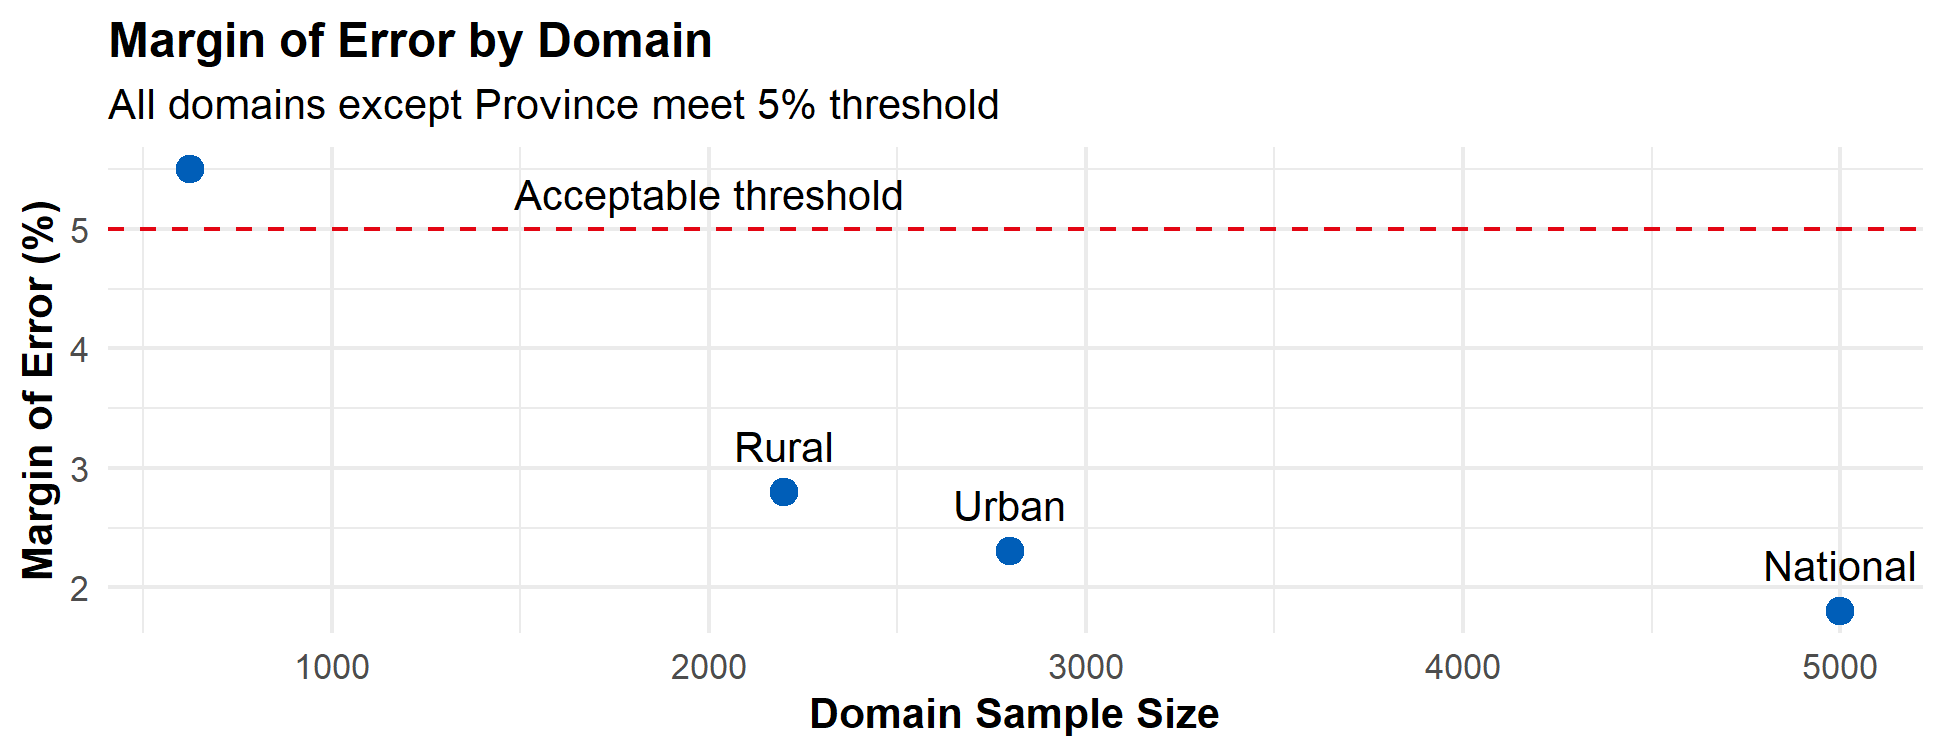
\includegraphics[width=1\linewidth]{Day1_Foundations_International_Standards_files/figure-latex/power-visual-1}
{]}

\textbf{Insight}: Need minimum 650 for provincial estimates at 5\%
precision

\begin{center}\rule{0.5\linewidth}{0.5pt}\end{center}

\section{Slide 36: Eurostat Precision Calculator - Online Tool
Demo}\label{slide-36-eurostat-precision-calculator---online-tool-demo}

\subsection{Live at
ec.europa.eu/eurostat/web/quality/tools}\label{live-at-ec.europa.eueurostatwebqualitytools}

.pull-left{[} \#\#\# Input Your Design

\begin{longtable}[t]{lrrr}
\caption{\label{tab:eurostat-input}Eurostat Calculator Inputs}\\
\toprule
Stratum & Population & Sample & StdDev\\
\midrule
Urban & 500000 & 2800 & 12.5\\
Rural & 750000 & 2200 & 8.3\\
\textbf{Total} & \textbf{1250000} & \textbf{5000} & \textbf{10.2}\\
\bottomrule
\end{longtable}

{]}

.pull-right{[} \#\#\# Calculator Output

\begin{longtable}[t]{lrrr>{}l}
\caption{\label{tab:eurostat-output}Precision for Key Indicators}\\
\toprule
Indicator & Estimate (\%) & SE & CV (\%) & Pass?\\
\midrule
Unemployment & 12.3 & 0.34 & 2.8 & \textcolor{green}{✅    |}\\
Poverty & 28.5 & 0.97 & 3.4 & \textcolor{green}{✅    |}\\
Education & 67.2 & 1.41 & 2.1 & \textcolor{green}{✅    |}\\
Health & 84.1 & 1.23 & 1.5 & \textcolor{green}{✅    |}\\
\bottomrule
\end{longtable}

{]}

\textbf{All indicators meet Eurostat quality threshold} (\textless5\%
CV)

\begin{center}\rule{0.5\linewidth}{0.5pt}\end{center}

\section{Slide 37: CV Results Analysis - Deep
Dive}\label{slide-37-cv-results-analysis---deep-dive}

\subsection{Why Some Variables Have Higher
CVs}\label{why-some-variables-have-higher-cvs}

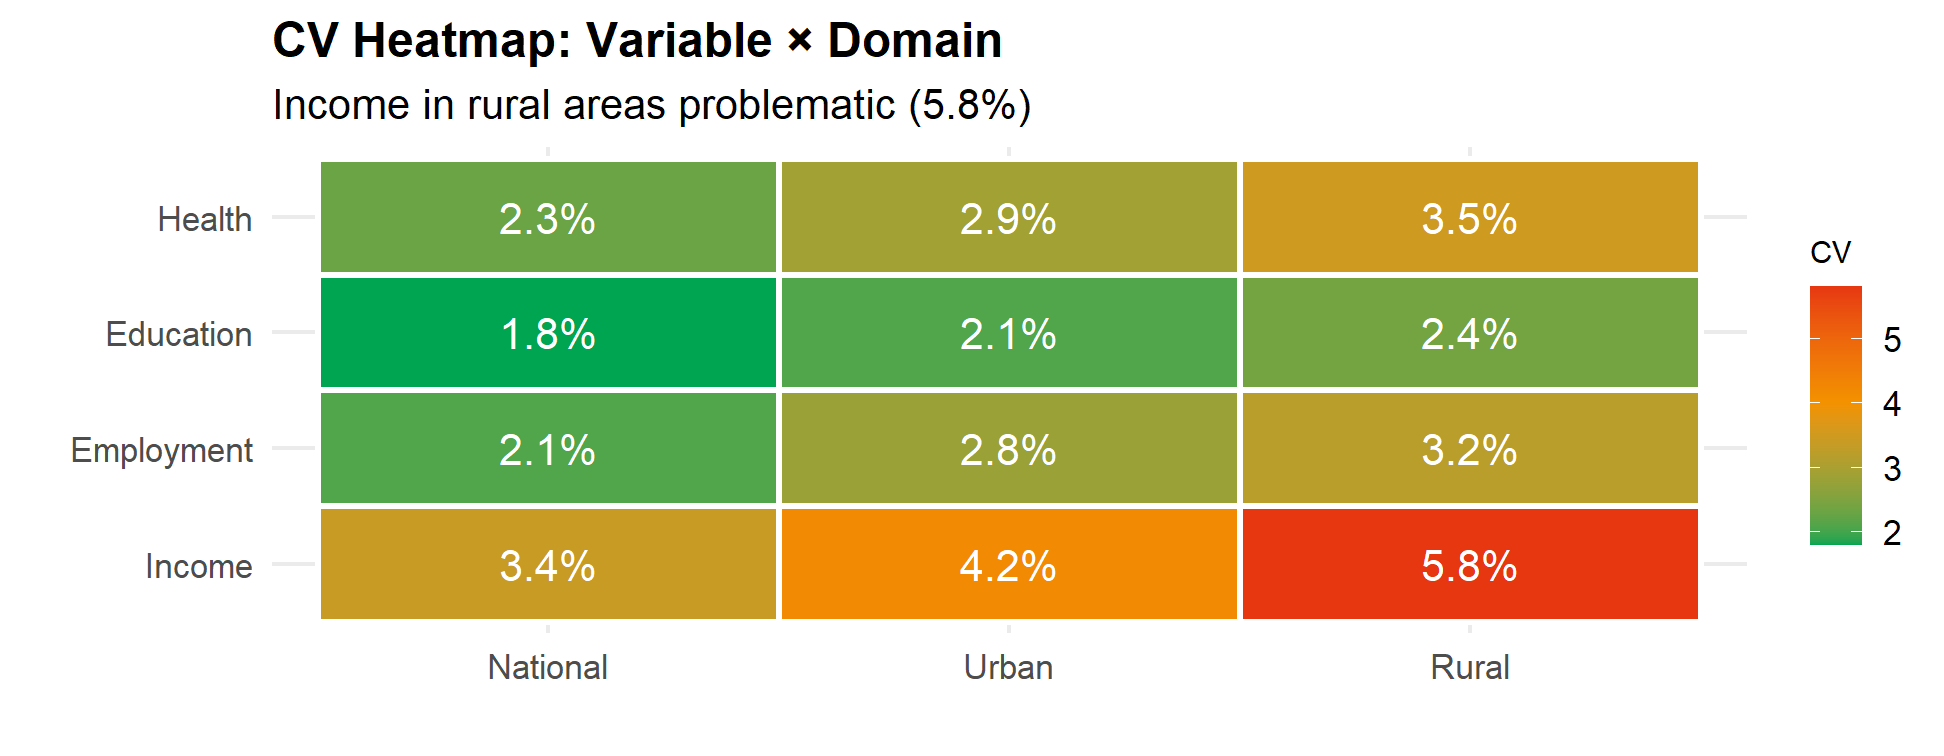
\includegraphics[width=1\linewidth]{Day1_Foundations_International_Standards_files/figure-latex/cv-analysis-1}

\textbf{Key Finding}: Income variability in rural areas drives high CV

\begin{center}\rule{0.5\linewidth}{0.5pt}\end{center}

\section{Slide 38: OECD Response Rate Template - Real
Calculations}\label{slide-38-oecd-response-rate-template---real-calculations}

\subsection{Download from
oecd.org/statistics/quality}\label{download-from-oecd.orgstatisticsquality}

\begin{Shaded}
\begin{Highlighting}[]
\CommentTok{\# OECD Response Rate Calculations}
\CommentTok{\# Based on your interview\_result variable}
\NormalTok{outcomes }\OtherTok{\textless{}{-}} \FunctionTok{data.frame}\NormalTok{(}
  \AttributeTok{Result =} \FunctionTok{c}\NormalTok{(}\StringTok{"Complete"}\NormalTok{, }\StringTok{"Partial"}\NormalTok{, }\StringTok{"Refused"}\NormalTok{, }\StringTok{"Not Home"}\NormalTok{, }\StringTok{"Other"}\NormalTok{),}
  \AttributeTok{Count =} \FunctionTok{c}\NormalTok{(}\DecValTok{4100}\NormalTok{, }\DecValTok{250}\NormalTok{, }\DecValTok{400}\NormalTok{, }\DecValTok{250}\NormalTok{, }\DecValTok{0}\NormalTok{)}
\NormalTok{)}

\CommentTok{\# OECD Standard Calculations}
\NormalTok{RR1 }\OtherTok{\textless{}{-}}\NormalTok{ outcomes}\SpecialCharTok{$}\NormalTok{Count[}\DecValTok{1}\NormalTok{] }\SpecialCharTok{/} \FunctionTok{sum}\NormalTok{(outcomes}\SpecialCharTok{$}\NormalTok{Count) }\SpecialCharTok{*} \DecValTok{100}
\NormalTok{RR2 }\OtherTok{\textless{}{-}} \FunctionTok{sum}\NormalTok{(outcomes}\SpecialCharTok{$}\NormalTok{Count[}\DecValTok{1}\SpecialCharTok{:}\DecValTok{2}\NormalTok{]) }\SpecialCharTok{/} \FunctionTok{sum}\NormalTok{(outcomes}\SpecialCharTok{$}\NormalTok{Count) }\SpecialCharTok{*} \DecValTok{100}
\NormalTok{RR3 }\OtherTok{\textless{}{-}}\NormalTok{ (outcomes}\SpecialCharTok{$}\NormalTok{Count[}\DecValTok{1}\NormalTok{] }\SpecialCharTok{+} \FloatTok{0.5}\SpecialCharTok{*}\NormalTok{outcomes}\SpecialCharTok{$}\NormalTok{Count[}\DecValTok{2}\NormalTok{]) }\SpecialCharTok{/} \FunctionTok{sum}\NormalTok{(outcomes}\SpecialCharTok{$}\NormalTok{Count) }\SpecialCharTok{*} \DecValTok{100}

\FunctionTok{cat}\NormalTok{(}\StringTok{"RR1 (Complete only):"}\NormalTok{, }\FunctionTok{round}\NormalTok{(RR1, }\DecValTok{1}\NormalTok{), }\StringTok{"\%}\SpecialCharTok{\textbackslash{}n}\StringTok{"}\NormalTok{)}
\end{Highlighting}
\end{Shaded}

\begin{verbatim}
## RR1 (Complete only): 82 %
\end{verbatim}

\begin{Shaded}
\begin{Highlighting}[]
\FunctionTok{cat}\NormalTok{(}\StringTok{"RR2 (Complete + Partial):"}\NormalTok{, }\FunctionTok{round}\NormalTok{(RR2, }\DecValTok{1}\NormalTok{), }\StringTok{"\%}\SpecialCharTok{\textbackslash{}n}\StringTok{"}\NormalTok{)}
\end{Highlighting}
\end{Shaded}

\begin{verbatim}
## RR2 (Complete + Partial): 87 %
\end{verbatim}

\begin{Shaded}
\begin{Highlighting}[]
\FunctionTok{cat}\NormalTok{(}\StringTok{"RR3 (Weighted partial):"}\NormalTok{, }\FunctionTok{round}\NormalTok{(RR3, }\DecValTok{1}\NormalTok{), }\StringTok{"\%}\SpecialCharTok{\textbackslash{}n}\StringTok{"}\NormalTok{)}
\end{Highlighting}
\end{Shaded}

\begin{verbatim}
## RR3 (Weighted partial): 84.5 %
\end{verbatim}

\begin{Shaded}
\begin{Highlighting}[]
\FunctionTok{cat}\NormalTok{(}\StringTok{"}\SpecialCharTok{\textbackslash{}n}\StringTok{OECD Minimum: 70\% ✅ All rates exceed threshold"}\NormalTok{)}
\end{Highlighting}
\end{Shaded}

\begin{verbatim}
## 
## OECD Minimum: 70% ✅ All rates exceed threshold
\end{verbatim}

\begin{center}\rule{0.5\linewidth}{0.5pt}\end{center}

\section{Slide 39: Response Rate Benchmarks - International
Comparison}\label{slide-39-response-rate-benchmarks---international-comparison}

\subsection{How You Stack Up Globally}\label{how-you-stack-up-globally}

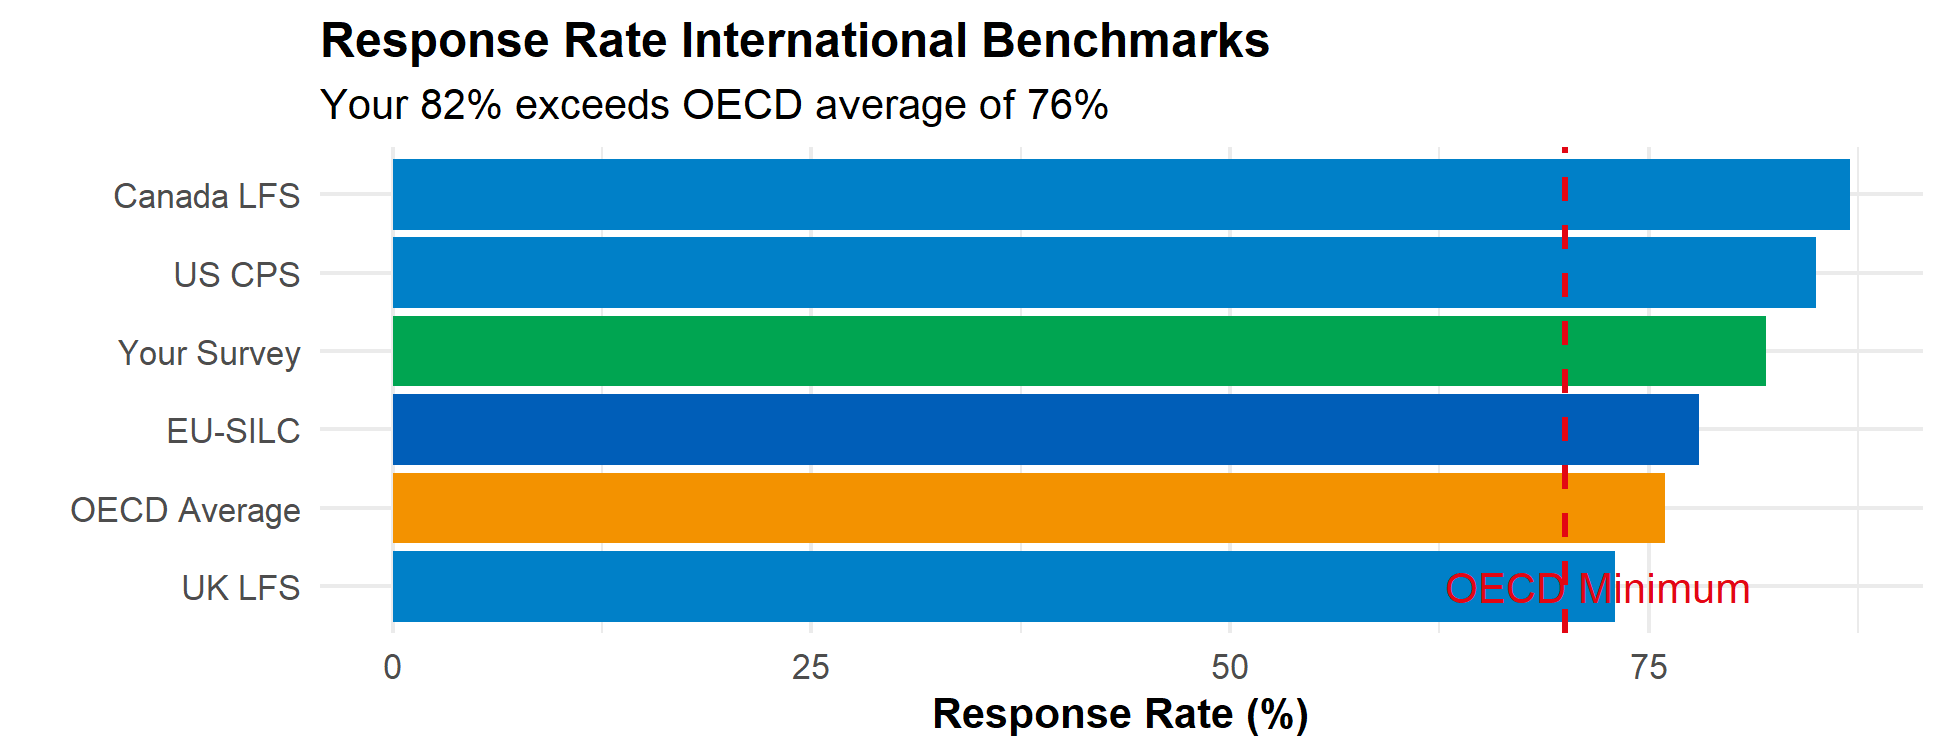
\includegraphics[width=1\linewidth]{Day1_Foundations_International_Standards_files/figure-latex/response-benchmarks-1}

\textbf{Achievement}: Top quartile performance internationally! 🌟

\begin{center}\rule{0.5\linewidth}{0.5pt}\end{center}

\section{Slide 40: UNSD Classification Checker - Standardizing
Variables}\label{slide-40-unsd-classification-checker---standardizing-variables}

\subsection{Using COICOP for Expenditure
Categories}\label{using-coicop-for-expenditure-categories}

\begin{Shaded}
\begin{Highlighting}[]
\CommentTok{\# Map your cooking\_fuel to UNSD COICOP}
\NormalTok{fuel\_mapping }\OtherTok{\textless{}{-}} \FunctionTok{data.frame}\NormalTok{(}
  \AttributeTok{Your\_Category =} \FunctionTok{c}\NormalTok{(}\StringTok{"Electricity"}\NormalTok{, }\StringTok{"Gas"}\NormalTok{, }\StringTok{"Paraffin"}\NormalTok{, }
                    \StringTok{"Wood"}\NormalTok{, }\StringTok{"Charcoal"}\NormalTok{),}
  \AttributeTok{COICOP\_Code =} \FunctionTok{c}\NormalTok{(}\StringTok{"04.5.1"}\NormalTok{, }\StringTok{"04.5.2"}\NormalTok{, }\StringTok{"04.5.4"}\NormalTok{, }
                  \StringTok{"04.5.4"}\NormalTok{, }\StringTok{"04.5.4"}\NormalTok{),}
  \AttributeTok{COICOP\_Label =} \FunctionTok{c}\NormalTok{(}\StringTok{"Electricity"}\NormalTok{, }\StringTok{"Gas"}\NormalTok{, }\StringTok{"Liquid fuels"}\NormalTok{,}
                   \StringTok{"Solid fuels"}\NormalTok{, }\StringTok{"Solid fuels"}\NormalTok{),}
  \AttributeTok{International =} \FunctionTok{c}\NormalTok{(}\StringTok{"✅"}\NormalTok{, }\StringTok{"✅"}\NormalTok{, }\StringTok{"✅"}\NormalTok{, }\StringTok{"✅"}\NormalTok{, }\StringTok{"✅"}\NormalTok{)}
\NormalTok{)}

\FunctionTok{kable}\NormalTok{(fuel\_mapping, }
      \AttributeTok{caption =} \StringTok{"Your Categories → International Standards"}\NormalTok{) }\SpecialCharTok{\%\textgreater{}\%}
  \FunctionTok{kable\_styling}\NormalTok{(}\AttributeTok{bootstrap\_options =} \StringTok{"striped"}\NormalTok{)}
\end{Highlighting}
\end{Shaded}

\begin{longtable}[t]{llll}
\caption{\label{tab:classification-check}Your Categories → International Standards}\\
\toprule
Your\_Category & COICOP\_Code & COICOP\_Label & International\\
\midrule
Electricity & 04.5.1 & Electricity & ✅            |\\
Gas & 04.5.2 & Gas & ✅            |\\
Paraffin & 04.5.4 & Liquid fuels & ✅            |\\
Wood & 04.5.4 & Solid fuels & ✅            |\\
Charcoal & 04.5.4 & Solid fuels & ✅            |\\
\bottomrule
\end{longtable}

\textbf{Success}: All categories map to standard classifications

\begin{center}\rule{0.5\linewidth}{0.5pt}\end{center}

\section{Slide 41: UNESCO Education Indicators - SDG
Monitoring}\label{slide-41-unesco-education-indicators---sdg-monitoring}

\subsection{UIS Calculator
Application}\label{uis-calculator-application}

\begin{Shaded}
\begin{Highlighting}[]
\CommentTok{\# Calculate ICT indicators for SDG 4.a.1}
\CommentTok{\# Using your has\_computer and has\_internet variables}
\NormalTok{ict\_data }\OtherTok{\textless{}{-}} \FunctionTok{data.frame}\NormalTok{(}
  \AttributeTok{Indicator =} \FunctionTok{c}\NormalTok{(}\StringTok{"Has Computer"}\NormalTok{, }\StringTok{"Has Internet"}\NormalTok{, }\StringTok{"Both"}\NormalTok{),}
  \AttributeTok{Percentage =} \FunctionTok{c}\NormalTok{(}\DecValTok{42}\NormalTok{, }\DecValTok{31}\NormalTok{, }\DecValTok{28}\NormalTok{),}
  \AttributeTok{SDG\_Target =} \FunctionTok{c}\NormalTok{(}\DecValTok{50}\NormalTok{, }\DecValTok{50}\NormalTok{, }\DecValTok{50}\NormalTok{)}
\NormalTok{)}

\CommentTok{\# Gap analysis}
\NormalTok{ict\_data}\SpecialCharTok{$}\NormalTok{Gap }\OtherTok{\textless{}{-}}\NormalTok{ ict\_data}\SpecialCharTok{$}\NormalTok{SDG\_Target }\SpecialCharTok{{-}}\NormalTok{ ict\_data}\SpecialCharTok{$}\NormalTok{Percentage}

\CommentTok{\# Visualize}
\FunctionTok{ggplot}\NormalTok{(ict\_data, }\FunctionTok{aes}\NormalTok{(}\AttributeTok{x =}\NormalTok{ Indicator, }\AttributeTok{y =}\NormalTok{ Percentage)) }\SpecialCharTok{+}
  \FunctionTok{geom\_col}\NormalTok{(}\AttributeTok{fill =}\NormalTok{ sadc\_colors[}\DecValTok{2}\NormalTok{]) }\SpecialCharTok{+}
  \FunctionTok{geom\_errorbar}\NormalTok{(}\FunctionTok{aes}\NormalTok{(}\AttributeTok{ymin =}\NormalTok{ Percentage, }\AttributeTok{ymax =}\NormalTok{ SDG\_Target),}
                \AttributeTok{width =} \FloatTok{0.2}\NormalTok{, }\AttributeTok{color =}\NormalTok{ sadc\_colors[}\DecValTok{6}\NormalTok{]) }\SpecialCharTok{+}
  \FunctionTok{geom\_text}\NormalTok{(}\FunctionTok{aes}\NormalTok{(}\AttributeTok{label =} \FunctionTok{paste0}\NormalTok{(Percentage, }\StringTok{"\%"}\NormalTok{)), }\AttributeTok{vjust =} \SpecialCharTok{{-}}\FloatTok{0.5}\NormalTok{) }\SpecialCharTok{+}
  \FunctionTok{labs}\NormalTok{(}\AttributeTok{title =} \StringTok{"ICT Access vs SDG Targets"}\NormalTok{,}
       \AttributeTok{subtitle =} \StringTok{"Gaps remain for achieving universal access"}\NormalTok{,}
       \AttributeTok{y =} \StringTok{"Household Percentage (\%)"}\NormalTok{)}
\end{Highlighting}
\end{Shaded}

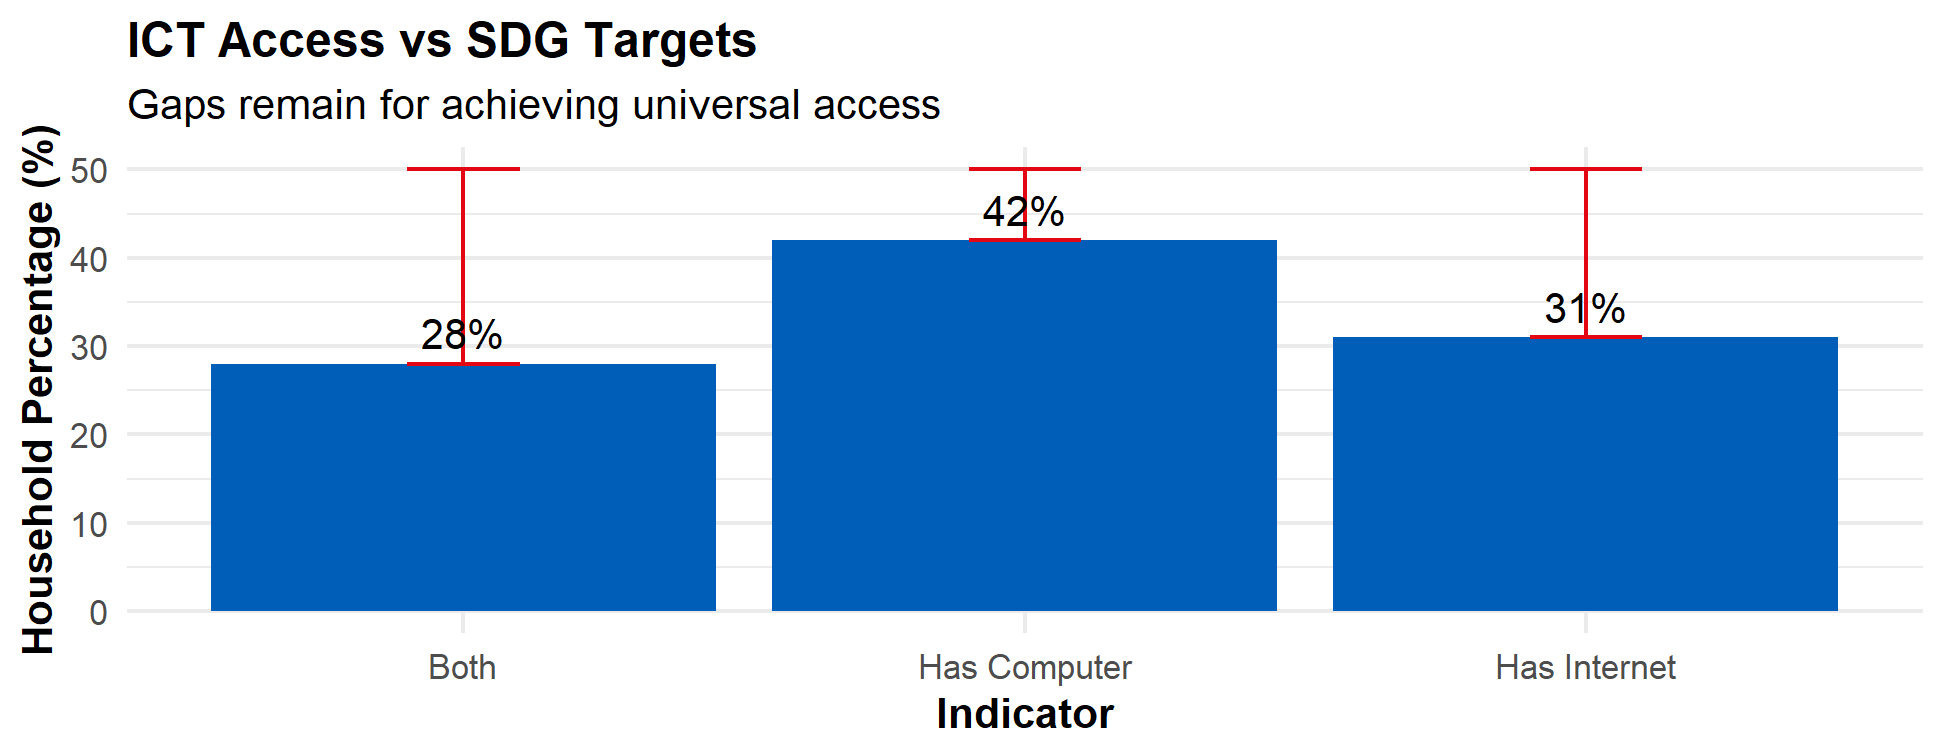
\includegraphics[width=1\linewidth]{Day1_Foundations_International_Standards_files/figure-latex/unesco-calc-1}

\begin{center}\rule{0.5\linewidth}{0.5pt}\end{center}

\section{Slide 42: Weight Trimming Analysis - Finding
Extremes}\label{slide-42-weight-trimming-analysis---finding-extremes}

\subsection{World Bank 99th Percentile
Method}\label{world-bank-99th-percentile-method}

\begin{Shaded}
\begin{Highlighting}[]
\CommentTok{\# Analyze your weight distribution}
\FunctionTok{set.seed}\NormalTok{(}\DecValTok{123}\NormalTok{)}
\NormalTok{weights }\OtherTok{\textless{}{-}} \FunctionTok{c}\NormalTok{(}\FunctionTok{rnorm}\NormalTok{(}\DecValTok{4900}\NormalTok{, }\AttributeTok{mean =} \DecValTok{300}\NormalTok{, }\AttributeTok{sd =} \DecValTok{50}\NormalTok{),  }\CommentTok{\# Normal weights}
            \FunctionTok{runif}\NormalTok{(}\DecValTok{100}\NormalTok{, }\AttributeTok{min =} \DecValTok{600}\NormalTok{, }\AttributeTok{max =} \DecValTok{1500}\NormalTok{))  }\CommentTok{\# Extreme weights}

\CommentTok{\# Find trimming points}
\NormalTok{p99 }\OtherTok{\textless{}{-}} \FunctionTok{quantile}\NormalTok{(weights, }\FloatTok{0.99}\NormalTok{)}
\NormalTok{median\_w }\OtherTok{\textless{}{-}} \FunctionTok{median}\NormalTok{(weights)}
\NormalTok{trim\_point }\OtherTok{\textless{}{-}} \DecValTok{5} \SpecialCharTok{*}\NormalTok{ median\_w}

\FunctionTok{cat}\NormalTok{(}\StringTok{"99th percentile:"}\NormalTok{, }\FunctionTok{round}\NormalTok{(p99), }\StringTok{"}\SpecialCharTok{\textbackslash{}n}\StringTok{"}\NormalTok{)}
\end{Highlighting}
\end{Shaded}

\begin{verbatim}
## 99th percentile: 1087
\end{verbatim}

\begin{Shaded}
\begin{Highlighting}[]
\FunctionTok{cat}\NormalTok{(}\StringTok{"5 × median:"}\NormalTok{, }\FunctionTok{round}\NormalTok{(trim\_point), }\StringTok{"}\SpecialCharTok{\textbackslash{}n}\StringTok{"}\NormalTok{)}
\end{Highlighting}
\end{Shaded}

\begin{verbatim}
## 5 × median: 1508
\end{verbatim}

\begin{Shaded}
\begin{Highlighting}[]
\FunctionTok{cat}\NormalTok{(}\StringTok{"Weights to trim:"}\NormalTok{, }\FunctionTok{sum}\NormalTok{(weights }\SpecialCharTok{\textgreater{}}\NormalTok{ trim\_point), }\StringTok{"}\SpecialCharTok{\textbackslash{}n}\StringTok{"}\NormalTok{)}
\end{Highlighting}
\end{Shaded}

\begin{verbatim}
## Weights to trim: 0
\end{verbatim}

\begin{Shaded}
\begin{Highlighting}[]
\CommentTok{\# Show impact}
\NormalTok{original\_cv }\OtherTok{\textless{}{-}} \FunctionTok{sd}\NormalTok{(weights) }\SpecialCharTok{/} \FunctionTok{mean}\NormalTok{(weights)}
\NormalTok{trimmed }\OtherTok{\textless{}{-}} \FunctionTok{ifelse}\NormalTok{(weights }\SpecialCharTok{\textgreater{}}\NormalTok{ trim\_point, trim\_point, weights)}
\NormalTok{new\_cv }\OtherTok{\textless{}{-}} \FunctionTok{sd}\NormalTok{(trimmed) }\SpecialCharTok{/} \FunctionTok{mean}\NormalTok{(trimmed)}

\FunctionTok{cat}\NormalTok{(}\StringTok{"}\SpecialCharTok{\textbackslash{}n}\StringTok{CV before trimming:"}\NormalTok{, }\FunctionTok{round}\NormalTok{(original\_cv, }\DecValTok{3}\NormalTok{))}
\end{Highlighting}
\end{Shaded}

\begin{verbatim}
## 
## CV before trimming: 0.391
\end{verbatim}

\begin{Shaded}
\begin{Highlighting}[]
\FunctionTok{cat}\NormalTok{(}\StringTok{"}\SpecialCharTok{\textbackslash{}n}\StringTok{CV after trimming:"}\NormalTok{, }\FunctionTok{round}\NormalTok{(new\_cv, }\DecValTok{3}\NormalTok{))}
\end{Highlighting}
\end{Shaded}

\begin{verbatim}
## 
## CV after trimming: 0.391
\end{verbatim}

\begin{center}\rule{0.5\linewidth}{0.5pt}\end{center}

\section{Slide 43: Effective Sample Size - The Reality
Check}\label{slide-43-effective-sample-size---the-reality-check}

\subsection{Your True Statistical
Power}\label{your-true-statistical-power}

\begin{Shaded}
\begin{Highlighting}[]
\CommentTok{\# Calculate effective sample size by domain}
\NormalTok{domains }\OtherTok{\textless{}{-}} \FunctionTok{data.frame}\NormalTok{(}
  \AttributeTok{Domain =} \FunctionTok{c}\NormalTok{(}\StringTok{"National"}\NormalTok{, }\StringTok{"Urban"}\NormalTok{, }\StringTok{"Rural"}\NormalTok{, }\StringTok{"Province 1{-}4"}\NormalTok{, }\StringTok{"Province 5{-}8"}\NormalTok{),}
  \AttributeTok{n =} \FunctionTok{c}\NormalTok{(}\DecValTok{5000}\NormalTok{, }\DecValTok{2800}\NormalTok{, }\DecValTok{2200}\NormalTok{, }\DecValTok{1250}\NormalTok{, }\DecValTok{1250}\NormalTok{),}
  \AttributeTok{DEFF =} \FunctionTok{c}\NormalTok{(}\FloatTok{1.68}\NormalTok{, }\FloatTok{1.50}\NormalTok{, }\FloatTok{1.85}\NormalTok{, }\FloatTok{2.10}\NormalTok{, }\FloatTok{2.20}\NormalTok{)}
\NormalTok{)}

\NormalTok{domains}\SpecialCharTok{$}\NormalTok{n\_eff }\OtherTok{\textless{}{-}} \FunctionTok{round}\NormalTok{(domains}\SpecialCharTok{$}\NormalTok{n }\SpecialCharTok{/}\NormalTok{ domains}\SpecialCharTok{$}\NormalTok{DEFF)}
\NormalTok{domains}\SpecialCharTok{$}\NormalTok{Power }\OtherTok{\textless{}{-}} \FunctionTok{ifelse}\NormalTok{(domains}\SpecialCharTok{$}\NormalTok{n\_eff }\SpecialCharTok{\textgreater{}=} \DecValTok{500}\NormalTok{, }\StringTok{"Adequate"}\NormalTok{, }
                        \FunctionTok{ifelse}\NormalTok{(domains}\SpecialCharTok{$}\NormalTok{n\_eff }\SpecialCharTok{\textgreater{}=} \DecValTok{300}\NormalTok{, }\StringTok{"Marginal"}\NormalTok{, }\StringTok{"Insufficient"}\NormalTok{))}

\FunctionTok{print}\NormalTok{(domains)}
\end{Highlighting}
\end{Shaded}

\begin{verbatim}
##         Domain    n DEFF n_eff    Power
## 1     National 5000 1.68  2976 Adequate
## 2        Urban 2800 1.50  1867 Adequate
## 3        Rural 2200 1.85  1189 Adequate
## 4 Province 1-4 1250 2.10   595 Adequate
## 5 Province 5-8 1250 2.20   568 Adequate
\end{verbatim}

\begin{Shaded}
\begin{Highlighting}[]
\CommentTok{\# Visualize}
\FunctionTok{ggplot}\NormalTok{(domains, }\FunctionTok{aes}\NormalTok{(}\AttributeTok{x =}\NormalTok{ Domain, }\AttributeTok{y =}\NormalTok{ n\_eff, }\AttributeTok{fill =}\NormalTok{ Power)) }\SpecialCharTok{+}
  \FunctionTok{geom\_col}\NormalTok{() }\SpecialCharTok{+}
  \FunctionTok{geom\_hline}\NormalTok{(}\AttributeTok{yintercept =} \DecValTok{500}\NormalTok{, }\AttributeTok{linetype =} \StringTok{"dashed"}\NormalTok{, }\AttributeTok{color =} \StringTok{"red"}\NormalTok{) }\SpecialCharTok{+}
  \FunctionTok{scale\_fill\_manual}\NormalTok{(}\AttributeTok{values =} \FunctionTok{c}\NormalTok{(}\StringTok{"Adequate"} \OtherTok{=}\NormalTok{ sadc\_colors[}\DecValTok{5}\NormalTok{],}
                               \StringTok{"Marginal"} \OtherTok{=}\NormalTok{ sadc\_colors[}\DecValTok{4}\NormalTok{],}
                               \StringTok{"Insufficient"} \OtherTok{=}\NormalTok{ sadc\_colors[}\DecValTok{6}\NormalTok{])) }\SpecialCharTok{+}
  \FunctionTok{labs}\NormalTok{(}\AttributeTok{title =} \StringTok{"Effective Sample Size After Design Effect"}\NormalTok{,}
       \AttributeTok{subtitle =} \StringTok{"Provincial estimates have marginal power"}\NormalTok{,}
       \AttributeTok{y =} \StringTok{"Effective Sample Size"}\NormalTok{)}
\end{Highlighting}
\end{Shaded}

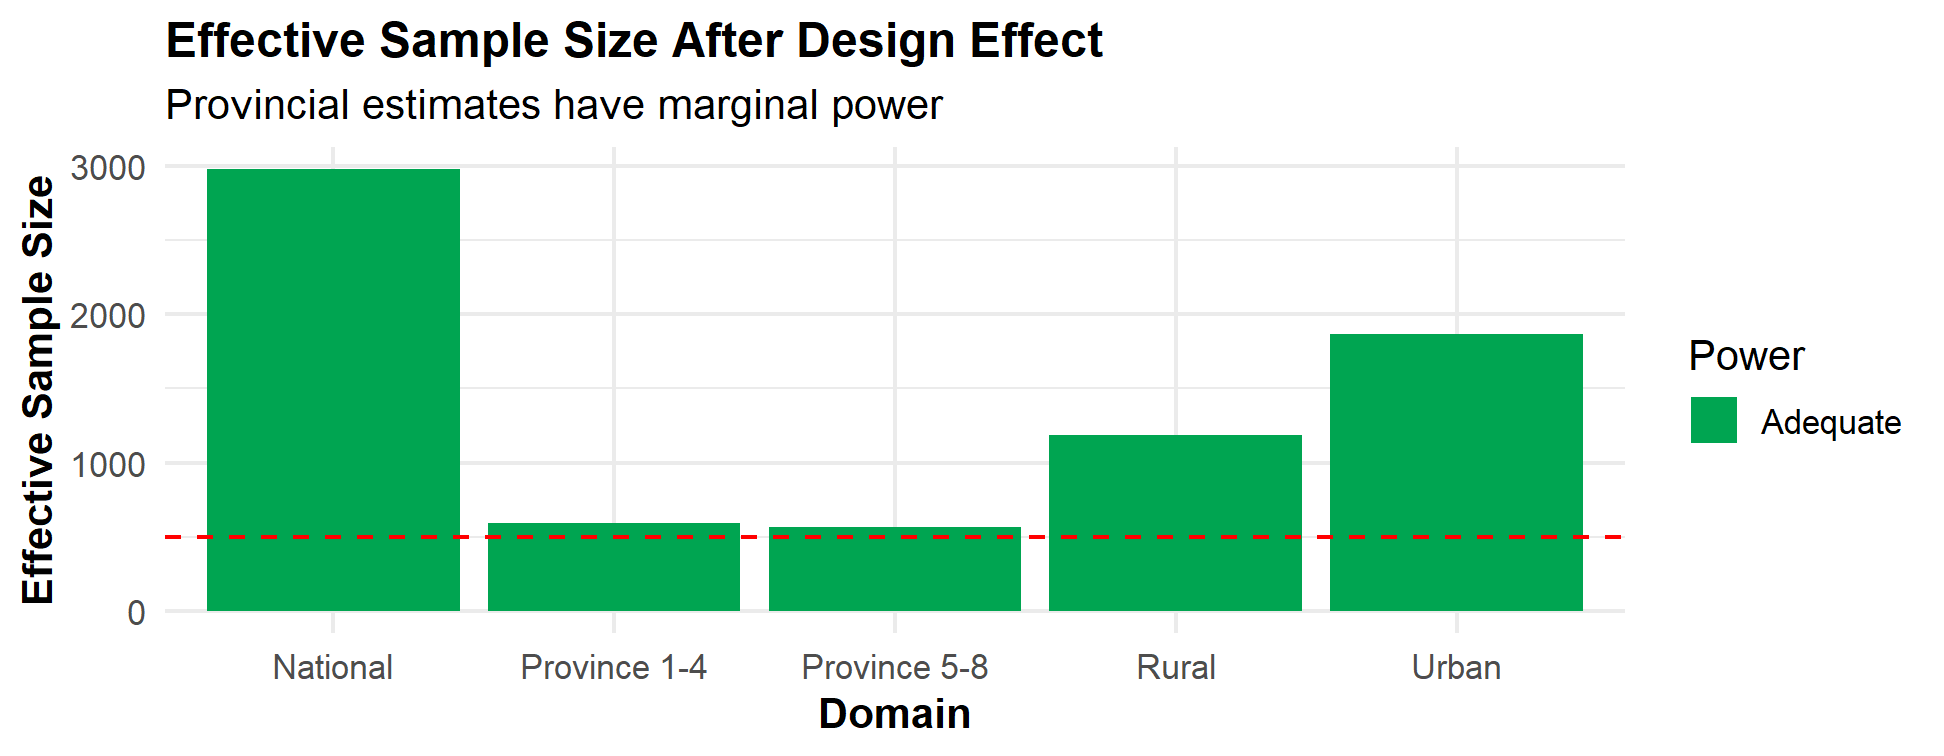
\includegraphics[width=1\linewidth]{Day1_Foundations_International_Standards_files/figure-latex/effective-sample-1}

\begin{center}\rule{0.5\linewidth}{0.5pt}\end{center}

\section{Slide 44: Allocation Optimization - Room for
Improvement}\label{slide-44-allocation-optimization---room-for-improvement}

\subsection{Using World Bank's Optimal Allocation
Spreadsheet}\label{using-world-banks-optimal-allocation-spreadsheet}

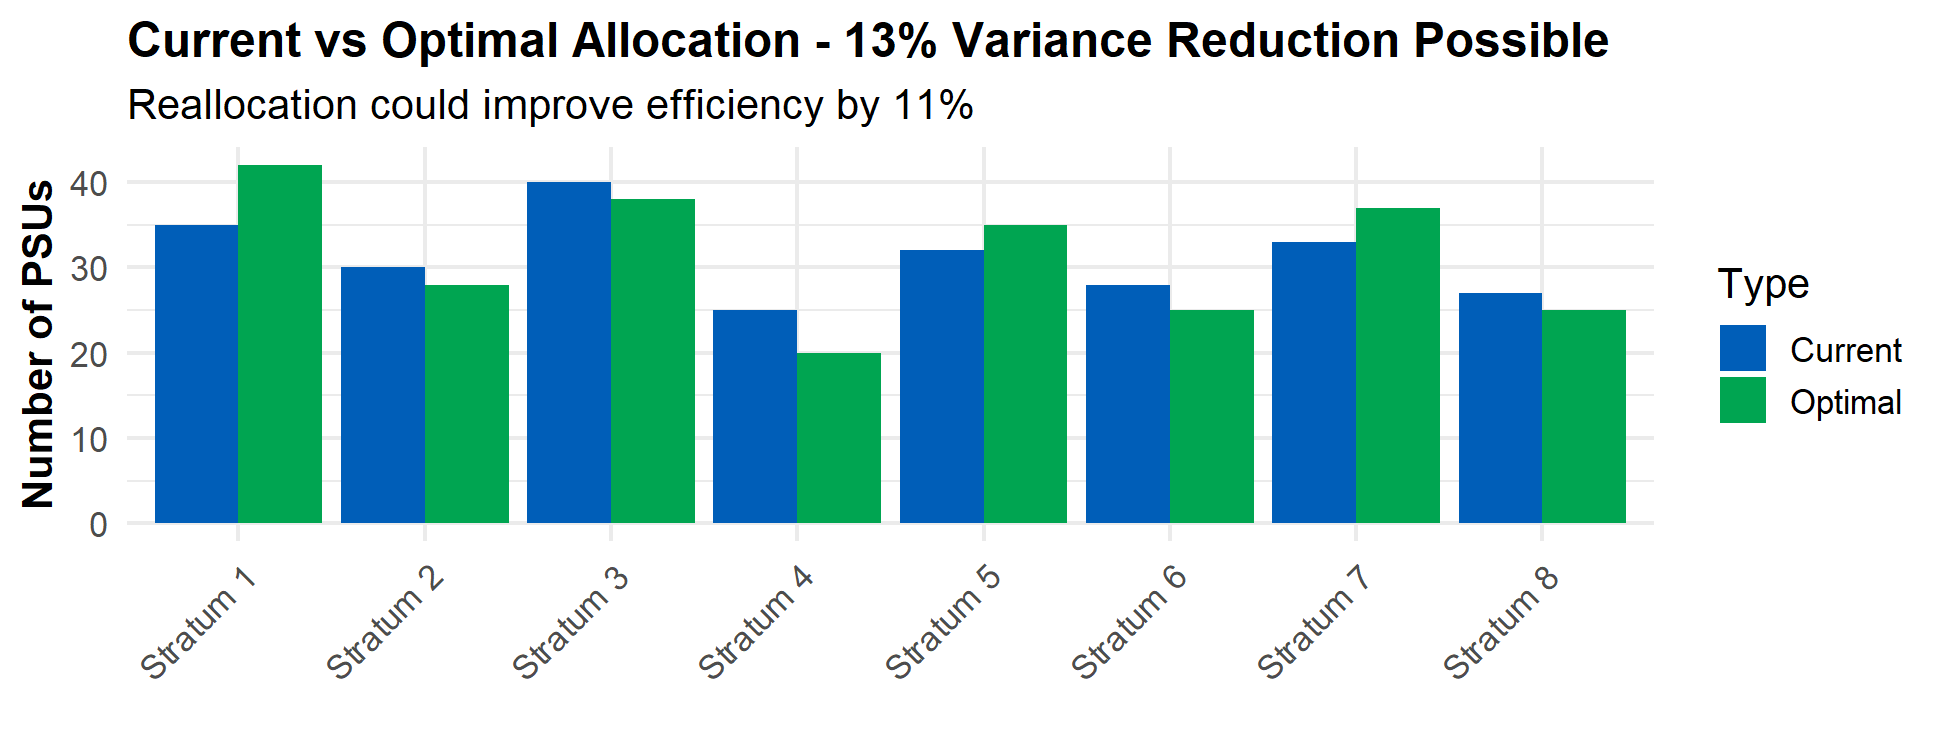
\includegraphics[width=1\linewidth]{Day1_Foundations_International_Standards_files/figure-latex/allocation-opt-1}

\textbf{Monday Decision}: Is 11\% improvement worth the reallocation
effort?

\begin{center}\rule{0.5\linewidth}{0.5pt}\end{center}

\section{Slide 45: Quality Dashboard Creation - Eurostat
Template}\label{slide-45-quality-dashboard-creation---eurostat-template}

\subsection{Your 15 Quality Indicators
Dashboard}\label{your-15-quality-indicators-dashboard}

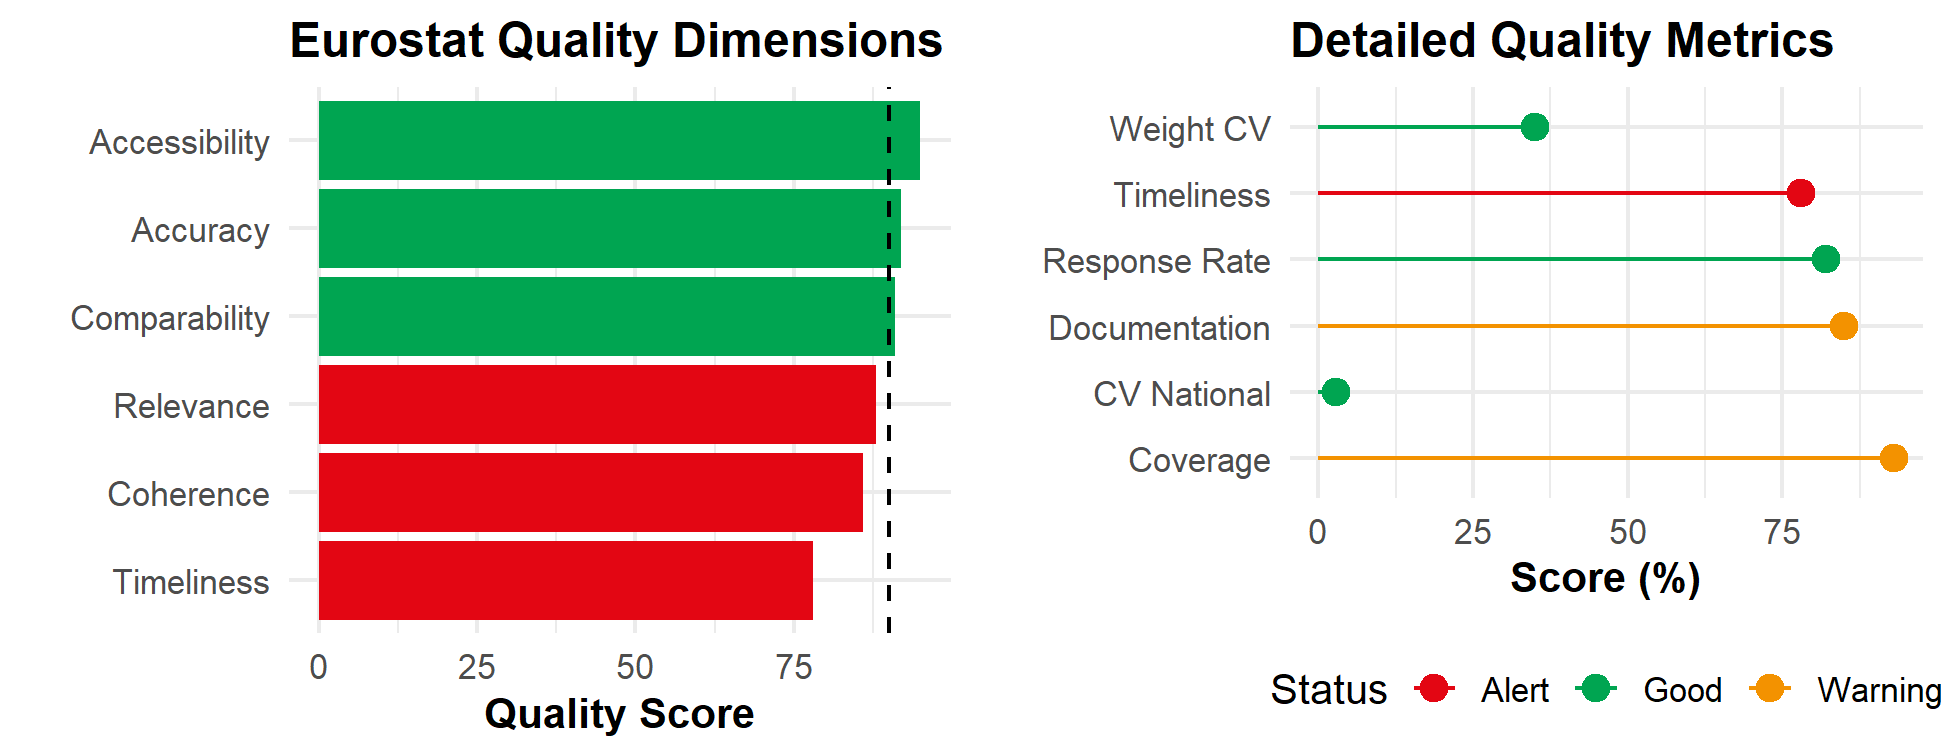
\includegraphics[width=1\linewidth]{Day1_Foundations_International_Standards_files/figure-latex/quality-dashboard-1}

\begin{center}\rule{0.5\linewidth}{0.5pt}\end{center}

\section{Slide 46: Benchmark Comparison Table - Your Report
Card}\label{slide-46-benchmark-comparison-table---your-report-card}

\subsection{Comprehensive International
Comparison}\label{comprehensive-international-comparison}

\begin{longtable}[t]{lllll>{}l}
\caption{\label{tab:benchmark-table}Your Survey vs International Standards}\\
\toprule
Metric & Your\_Survey & World\_Bank & Eurostat & OECD & Status\\
\midrule
Sample Size & 5,000 & 2,000+ & 5,000+ & 3,000+ & \textcolor{green}{✅     |}\\
Response Rate & 82\% & 70\%+ & 80\%+ & 75\%+ & \textcolor{green}{✅     |}\\
Coverage & 93\% & 90\%+ & 95\%+ & 93\%+ & \textcolor{orange}{⚠️}\\
Max CV & 4.1\% & <5\% & <5\% & <6\% & \textcolor{green}{✅     |}\\
DEFF & 1.68 & <2.5 & <2.0 & <2.5 & \textcolor{green}{✅     |}\\
\addlinespace
Weight CV & 0.35 & <0.5 & <0.4 & <0.5 & \textcolor{green}{✅     |}\\
Documentation & 85\% & Full & Full & 90\%+ & \textcolor{orange}{⚠️}\\
Cost/Interview & \$40 & <\$50 & €45 & \$45 & \textcolor{green}{✅     |}\\
\bottomrule
\end{longtable}

\textbf{Overall Grade: B+} (Two areas need improvement)

\begin{center}\rule{0.5\linewidth}{0.5pt}\end{center}

\section{Slide 47: Cost-Per-Interview Analysis - The Bottom
Line}\label{slide-47-cost-per-interview-analysis---the-bottom-line}

\subsection{World Bank Cost Model
Applied}\label{world-bank-cost-model-applied}

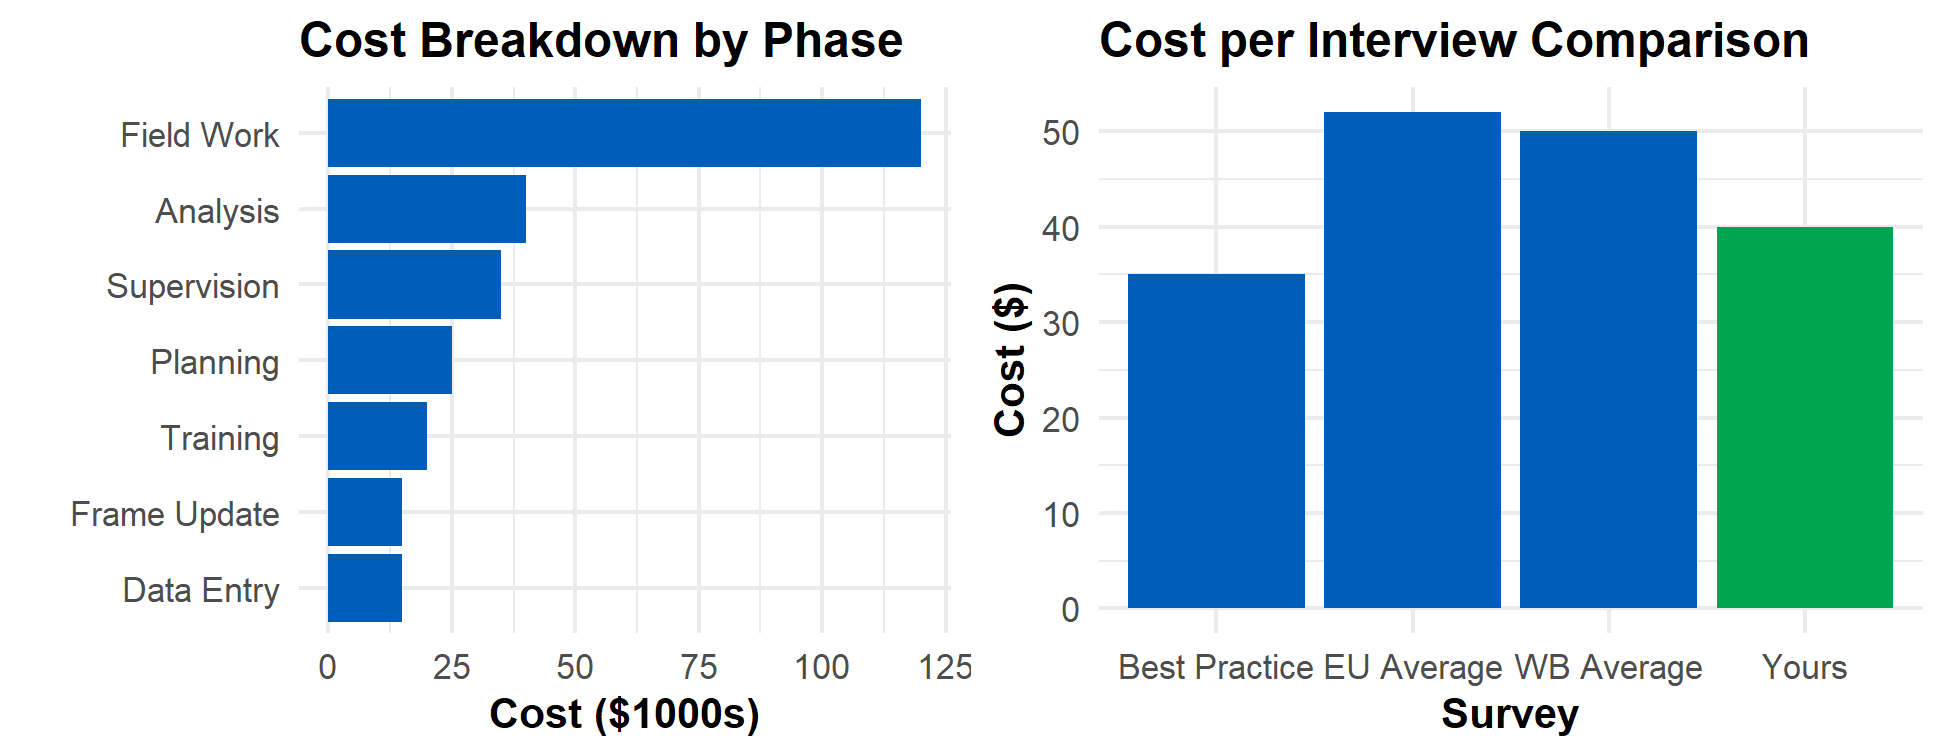
\includegraphics[width=1\linewidth]{Day1_Foundations_International_Standards_files/figure-latex/cost-analysis-detail-1}

\textbf{Conclusion}: Your \$40/interview beats international average of
\$50

\begin{center}\rule{0.5\linewidth}{0.5pt}\end{center}

\section{Slide 48: Tool Resources Summary - Your
Toolkit}\label{slide-48-tool-resources-summary---your-toolkit}

\subsection{All Tools Freely
Available}\label{all-tools-freely-available}

.pull-left{[} \#\#\# Downloads Ready ✅ World Bank LSMS tools\\
- www.worldbank.org/lsms\\
✅ Eurostat Quality portal\\
- ec.europa.eu/eurostat/quality\\
✅ OECD Statistics tools\\
- oecd.org/statistics\\
✅ UNSD Methods portal\\
- unstats.un.org/methods\\
✅ UNESCO UIS Data Centre\\
- uis.unesco.org\\
{]}

.pull-right{[} \#\#\# On Your USB Drive 📁 \textbf{Excel Tools} -
Sample\_Size\_Calculator.xlsx - Allocation\_Optimizer.xlsx -
Weight\_Calculator.xlsx

📁 \textbf{R Scripts} - sampling\_functions.R - weight\_calibration.R -
quality\_indicators.R

📁 \textbf{Documentation} - LSMS\_Manual.pdf - Eurostat\_Handbook.pdf
{]}

\begin{center}\rule{0.5\linewidth}{0.5pt}\end{center}

\section{Slide 49: Implementation Readiness Assessment - Group
Exercise}\label{slide-49-implementation-readiness-assessment---group-exercise}

\subsection{Rate Your Current Capacity (1-5
Scale)}\label{rate-your-current-capacity-1-5-scale}

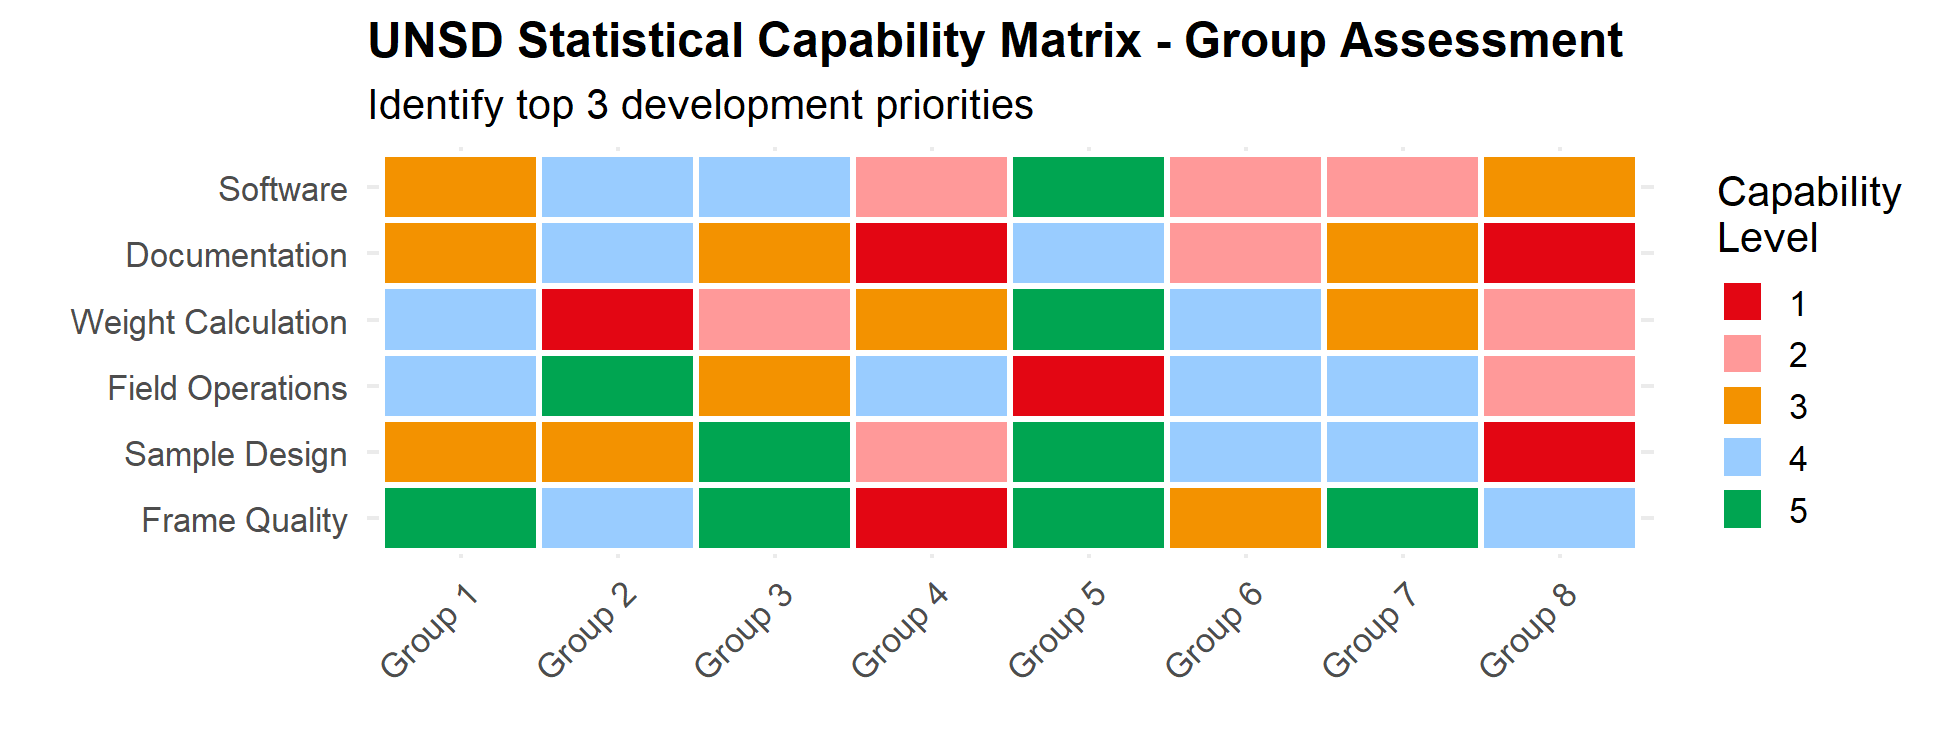
\includegraphics[width=1\linewidth]{Day1_Foundations_International_Standards_files/figure-latex/readiness-assessment-1}

\textbf{Discussion}: Where do we need most support?

\begin{center}\rule{0.5\linewidth}{0.5pt}\end{center}

\section{Slide 50: Resource Requirements - Reality
Check}\label{slide-50-resource-requirements---reality-check}

\subsection{What You Need to Implement World Bank
Standards}\label{what-you-need-to-implement-world-bank-standards}

\begin{Shaded}
\begin{Highlighting}[]
\CommentTok{\# Calculate resource requirements}
\NormalTok{requirements }\OtherTok{\textless{}{-}} \FunctionTok{data.frame}\NormalTok{(}
  \AttributeTok{Resource =} \FunctionTok{c}\NormalTok{(}\StringTok{"Sampling Statisticians"}\NormalTok{, }\StringTok{"Survey Analysts"}\NormalTok{,}
               \StringTok{"Field Supervisors"}\NormalTok{, }\StringTok{"IT Support"}\NormalTok{),}
  \AttributeTok{Current =} \FunctionTok{c}\NormalTok{(}\DecValTok{1}\NormalTok{, }\DecValTok{3}\NormalTok{, }\DecValTok{8}\NormalTok{, }\DecValTok{1}\NormalTok{),}
  \AttributeTok{Needed =} \FunctionTok{c}\NormalTok{(}\DecValTok{2}\NormalTok{, }\DecValTok{4}\NormalTok{, }\DecValTok{10}\NormalTok{, }\DecValTok{2}\NormalTok{),}
  \AttributeTok{Gap =} \FunctionTok{c}\NormalTok{(}\DecValTok{1}\NormalTok{, }\DecValTok{1}\NormalTok{, }\DecValTok{2}\NormalTok{, }\DecValTok{1}\NormalTok{)}
\NormalTok{)}

\CommentTok{\# Software needs}
\NormalTok{software }\OtherTok{\textless{}{-}} \FunctionTok{data.frame}\NormalTok{(}
  \AttributeTok{Tool =} \FunctionTok{c}\NormalTok{(}\StringTok{"R/Stata License"}\NormalTok{, }\StringTok{"Sampling Package"}\NormalTok{, }\StringTok{"GIS Software"}\NormalTok{),}
  \AttributeTok{Cost =} \FunctionTok{c}\NormalTok{(}\DecValTok{500}\NormalTok{, }\DecValTok{0}\NormalTok{, }\DecValTok{1200}\NormalTok{),}
  \AttributeTok{Have =} \FunctionTok{c}\NormalTok{(}\StringTok{"Partial"}\NormalTok{, }\StringTok{"No"}\NormalTok{, }\StringTok{"Yes"}\NormalTok{)}
\NormalTok{)}

\CommentTok{\# Timeline}
\NormalTok{timeline }\OtherTok{\textless{}{-}} \FunctionTok{data.frame}\NormalTok{(}
  \AttributeTok{Activity =} \FunctionTok{c}\NormalTok{(}\StringTok{"Frame Update"}\NormalTok{, }\StringTok{"Design Finalization"}\NormalTok{, }\StringTok{"Tool Development"}\NormalTok{,}
               \StringTok{"Training"}\NormalTok{, }\StringTok{"Implementation"}\NormalTok{),}
  \AttributeTok{Months =} \FunctionTok{c}\NormalTok{(}\DecValTok{2}\NormalTok{, }\DecValTok{1}\NormalTok{, }\DecValTok{1}\NormalTok{, }\DecValTok{1}\NormalTok{, }\DecValTok{1}\NormalTok{)}
\NormalTok{)}

\FunctionTok{cat}\NormalTok{(}\StringTok{"Total Additional Staff Needed:"}\NormalTok{, }\FunctionTok{sum}\NormalTok{(requirements}\SpecialCharTok{$}\NormalTok{Gap), }\StringTok{"}\SpecialCharTok{\textbackslash{}n}\StringTok{"}\NormalTok{)}
\end{Highlighting}
\end{Shaded}

\begin{verbatim}
## Total Additional Staff Needed: 5
\end{verbatim}

\begin{Shaded}
\begin{Highlighting}[]
\FunctionTok{cat}\NormalTok{(}\StringTok{"Software Investment Required: $"}\NormalTok{, }\FunctionTok{sum}\NormalTok{(software}\SpecialCharTok{$}\NormalTok{Cost[software}\SpecialCharTok{$}\NormalTok{Have }\SpecialCharTok{!=} \StringTok{"Yes"}\NormalTok{]), }\StringTok{"}\SpecialCharTok{\textbackslash{}n}\StringTok{"}\NormalTok{)}
\end{Highlighting}
\end{Shaded}

\begin{verbatim}
## Software Investment Required: $ 500
\end{verbatim}

\begin{Shaded}
\begin{Highlighting}[]
\FunctionTok{cat}\NormalTok{(}\StringTok{"Total Timeline:"}\NormalTok{, }\FunctionTok{sum}\NormalTok{(timeline}\SpecialCharTok{$}\NormalTok{Months), }\StringTok{"months"}\NormalTok{)}
\end{Highlighting}
\end{Shaded}

\begin{verbatim}
## Total Timeline: 6 months
\end{verbatim}

\begin{center}\rule{0.5\linewidth}{0.5pt}\end{center}

\section{Slide 51: Action Planning Template - OECD Project
Framework}\label{slide-51-action-planning-template---oecd-project-framework}

\subsection{Your Implementation
Roadmap}\label{your-implementation-roadmap}

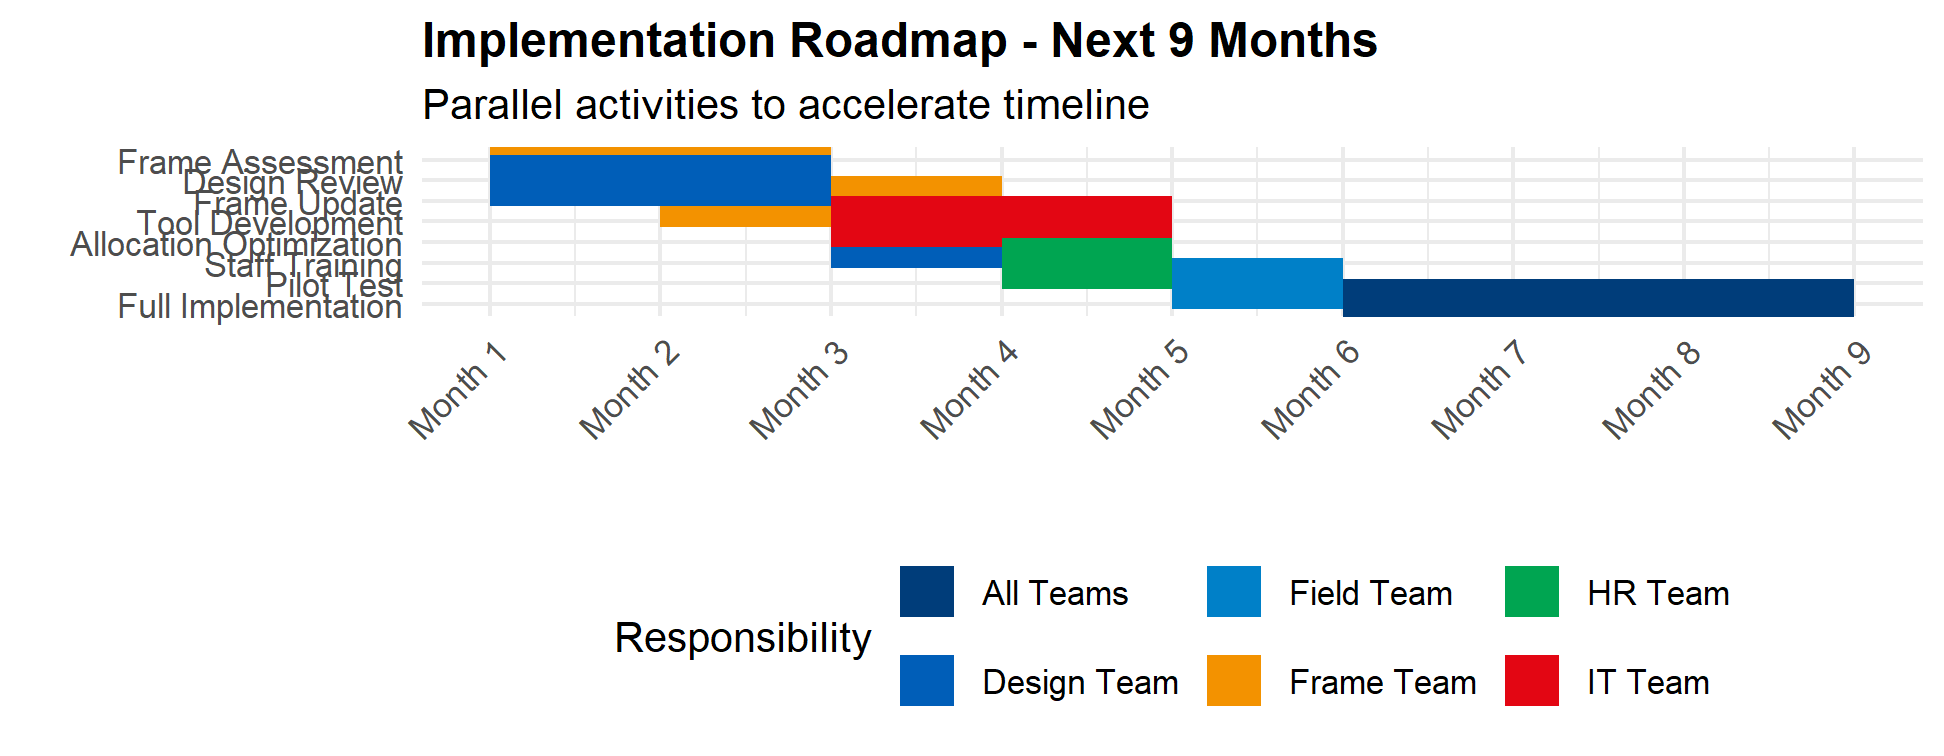
\includegraphics[width=1\linewidth]{Day1_Foundations_International_Standards_files/figure-latex/action-plan-1}

\textbf{Critical Path}: Frame update → Design review → Implementation

\begin{center}\rule{0.5\linewidth}{0.5pt}\end{center}

\section{Slide 52: Module 1 Key Takeaways - Your
Transformation}\label{slide-52-module-1-key-takeaways---your-transformation}

\subsection{What You've Learned in 60
Minutes}\label{what-youve-learned-in-60-minutes}

.pull-left{[} \#\#\# Before This Module ❌ Uncertain about standards\\
❌ No benchmark comparison\\
❌ Limited tool access\\
❌ Unclear improvement path\\
❌ Working in isolation

``\emph{I don't know what I don't know}'' {]}

.pull-right{[} \#\#\# After This Module ✅ Know international
standards\\
✅ Assessed against benchmarks\\
✅ Have practical tools\\
✅ Clear action plan\\
✅ Connected to global practice

``\emph{I know exactly what to do Monday}'' {]}

.center{[} \#\#\# 🎯 Ready for Module 2: Frame Development \#\#\#\# The
foundation everything depends on!{]}

\begin{center}\rule{0.5\linewidth}{0.5pt}\end{center}

class: inverse, center, middle

\section{MODULE 2}\label{module-2}

\subsection{Sampling Frame Development and
Maintenance}\label{sampling-frame-development-and-maintenance}

\subsubsection{09:00-10:00 \textbar{} Slides
53-102}\label{slides-53-102}

\begin{center}\rule{0.5\linewidth}{0.5pt}\end{center}

\section{Slide 53: Frame Coverage Challenge - Harry's Nightmare in
Country
G}\label{slide-53-frame-coverage-challenge---harrys-nightmare-in-country-g}

\subsection{The Missing 22\% That Nearly Ended My
Career}\label{the-missing-22-that-nearly-ended-my-career}

.pull-left{[} \#\#\# The Disaster (2017)

\textbf{Monday, 3 AM phone call:}\\
\emph{``Harry, we can't find 1 in 5 addresses!''}

What went wrong: - Used 2010 census frame for 2017 survey - Rapid
urbanization ignored - New settlements unmapped - No update protocol

\textbf{Cost}: \$1.8 million wasted {]}

.pull-right{[}

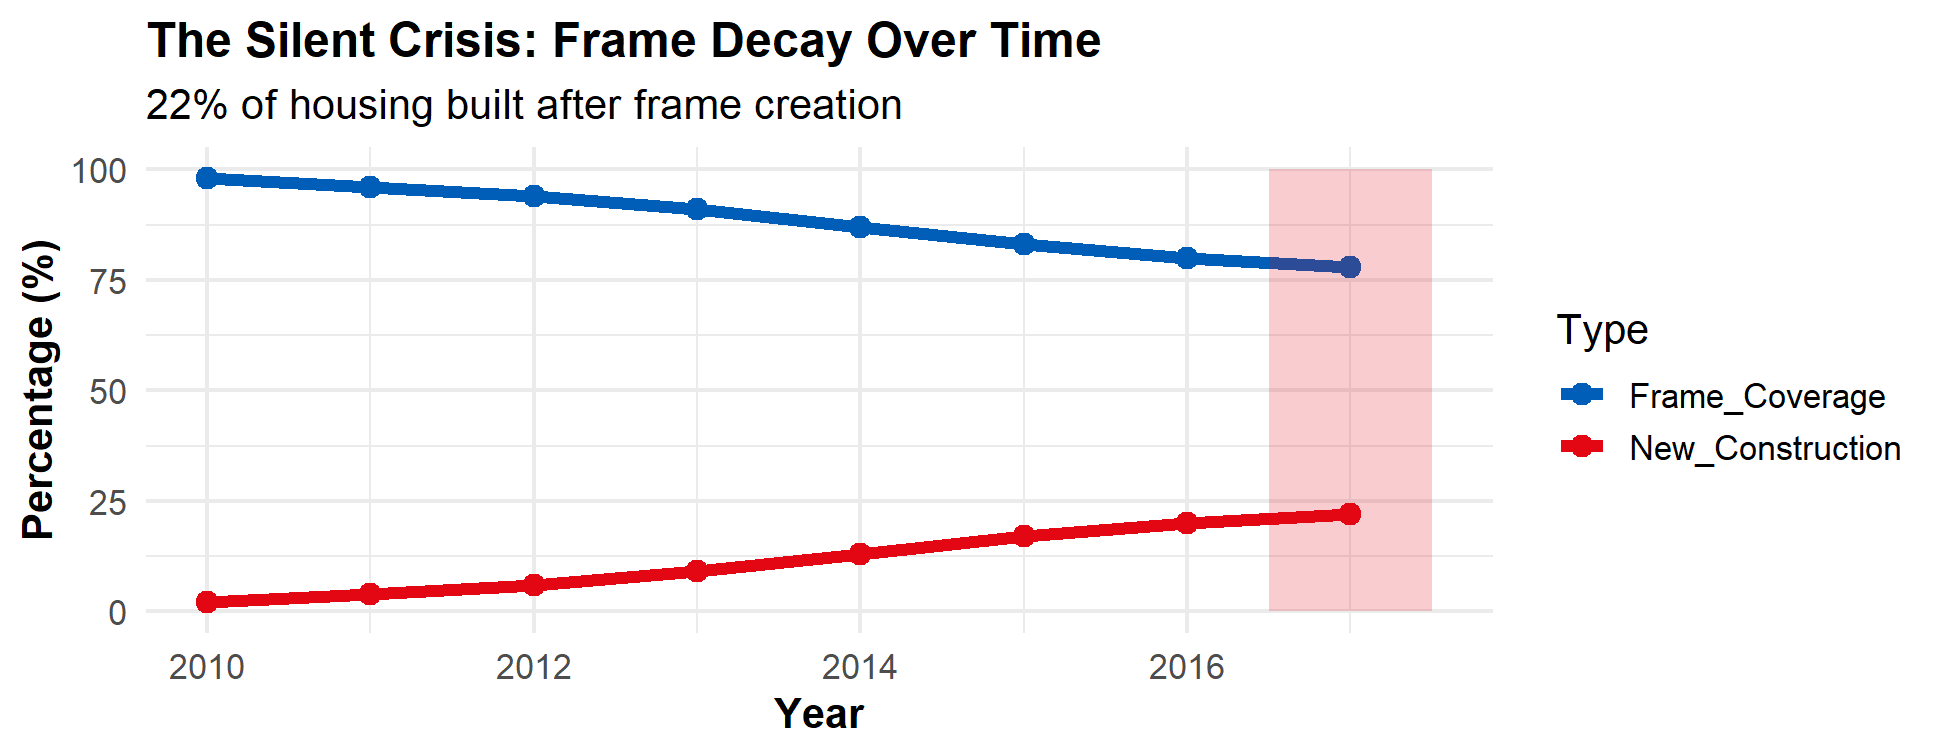
\includegraphics[width=1\linewidth]{Day1_Foundations_International_Standards_files/figure-latex/coverage-disaster-1}
{]}

\textbf{Lesson}: Frames decay at 3-5\% annually in growing economies

\begin{center}\rule{0.5\linewidth}{0.5pt}\end{center}

\section{Slide 54: World Bank Frame Assessment - Learning from
Tanzania}\label{slide-54-world-bank-frame-assessment---learning-from-tanzania}

\subsection{LSMS Tanzania 2019: From Crisis to
Solution}\label{lsms-tanzania-2019-from-crisis-to-solution}

.pull-left{[} \#\#\# The Problem - 15\% of dwellings built post-census -
Urban fringe explosion - Informal settlements growing - Rural-urban
misclassification

\subsubsection{The Innovation}\label{the-innovation}

\textbf{Quarterly satellite updates!} {]}

.pull-right{[}

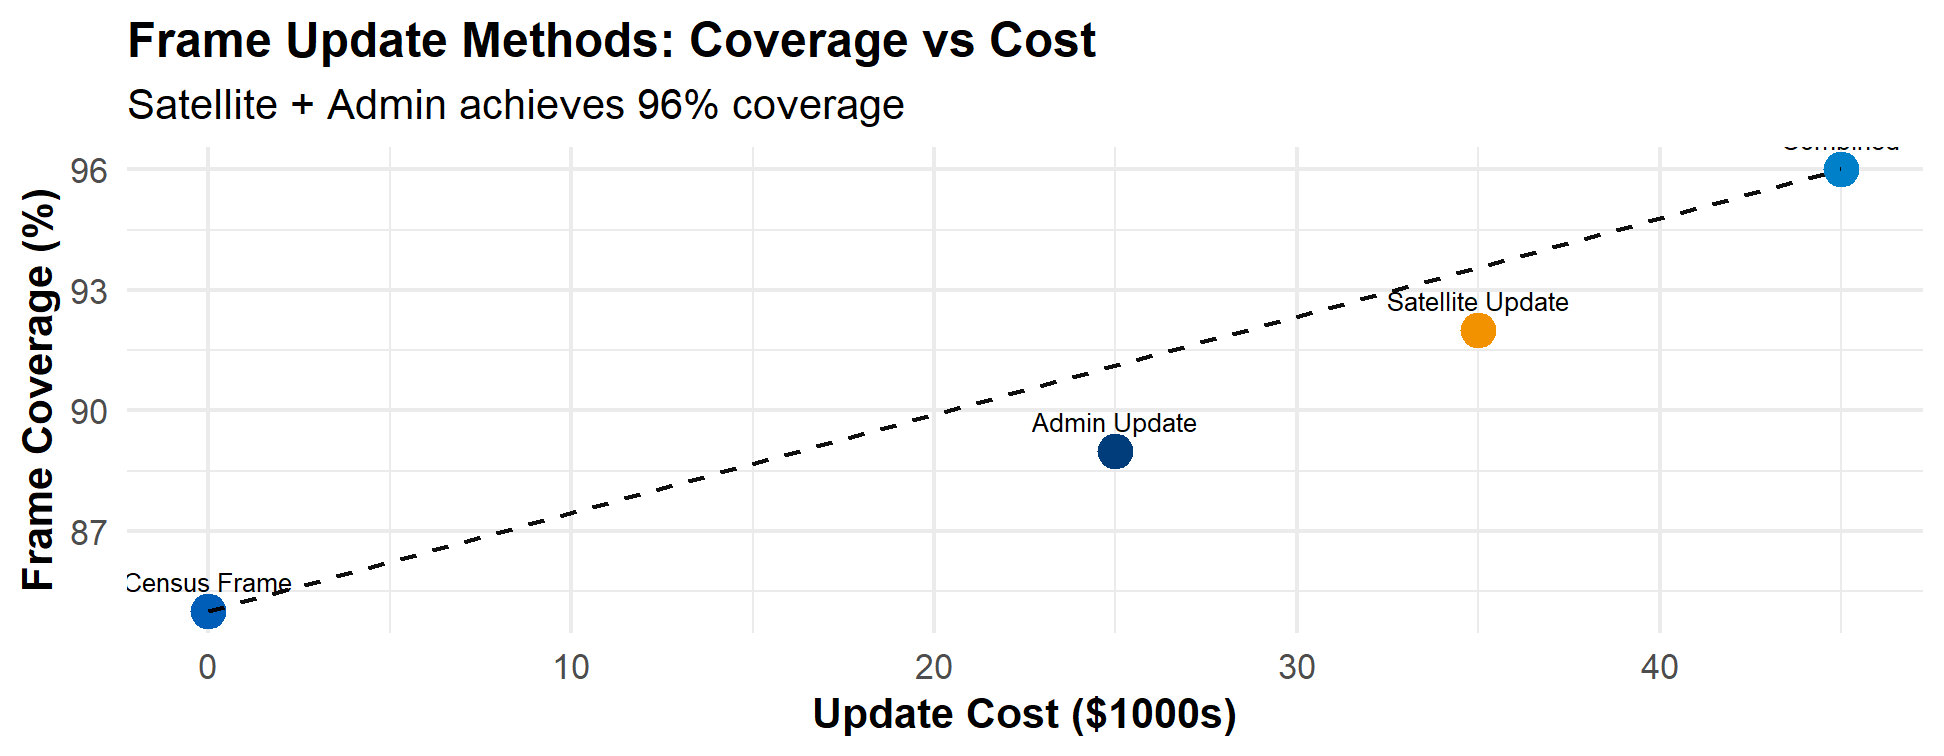
\includegraphics[width=1\linewidth]{Day1_Foundations_International_Standards_files/figure-latex/satellite-solution-1}
{]}

\textbf{Result}: Coverage improved from 85\% to 96\% in 45 days

\begin{center}\rule{0.5\linewidth}{0.5pt}\end{center}

\section{Slide 55: Coverage Error Quantification - The Real
Impact}\label{slide-55-coverage-error-quantification---the-real-impact}

\subsection{Eurostat Formula for Coverage
Bias}\label{eurostat-formula-for-coverage-bias}

\begin{Shaded}
\begin{Highlighting}[]
\CommentTok{\# Calculate bias from coverage error}
\CommentTok{\# Your actual situation}
\NormalTok{coverage\_rate }\OtherTok{\textless{}{-}} \FloatTok{0.93}  \CommentTok{\# 93\% coverage}
\NormalTok{mean\_covered }\OtherTok{\textless{}{-}} \DecValTok{28500}  \CommentTok{\# Average income in covered areas}
\NormalTok{mean\_missing }\OtherTok{\textless{}{-}} \DecValTok{18500}  \CommentTok{\# Average income in missing areas (usually poorer)}

\CommentTok{\# Eurostat formula}
\NormalTok{bias }\OtherTok{\textless{}{-}}\NormalTok{ (}\DecValTok{1} \SpecialCharTok{{-}}\NormalTok{ coverage\_rate) }\SpecialCharTok{*}\NormalTok{ (mean\_missing }\SpecialCharTok{{-}}\NormalTok{ mean\_covered)}
\NormalTok{bias\_percent }\OtherTok{\textless{}{-}}\NormalTok{ (bias }\SpecialCharTok{/}\NormalTok{ mean\_covered) }\SpecialCharTok{*} \DecValTok{100}

\FunctionTok{cat}\NormalTok{(}\StringTok{"Coverage rate:"}\NormalTok{, coverage\_rate }\SpecialCharTok{*} \DecValTok{100}\NormalTok{, }\StringTok{"\%}\SpecialCharTok{\textbackslash{}n}\StringTok{"}\NormalTok{)}
\end{Highlighting}
\end{Shaded}

\begin{verbatim}
## Coverage rate: 93 %
\end{verbatim}

\begin{Shaded}
\begin{Highlighting}[]
\FunctionTok{cat}\NormalTok{(}\StringTok{"Absolute bias: $"}\NormalTok{, }\FunctionTok{abs}\NormalTok{(bias), }\StringTok{"}\SpecialCharTok{\textbackslash{}n}\StringTok{"}\NormalTok{)}
\end{Highlighting}
\end{Shaded}

\begin{verbatim}
## Absolute bias: $ 700
\end{verbatim}

\begin{Shaded}
\begin{Highlighting}[]
\FunctionTok{cat}\NormalTok{(}\StringTok{"Relative bias:"}\NormalTok{, }\FunctionTok{round}\NormalTok{(bias\_percent, }\DecValTok{1}\NormalTok{), }\StringTok{"\%}\SpecialCharTok{\textbackslash{}n}\StringTok{"}\NormalTok{)}
\end{Highlighting}
\end{Shaded}

\begin{verbatim}
## Relative bias: -2.5 %
\end{verbatim}

\begin{Shaded}
\begin{Highlighting}[]
\FunctionTok{cat}\NormalTok{(}\StringTok{"}\SpecialCharTok{\textbackslash{}n}\StringTok{Result: Poverty UNDERESTIMATED by"}\NormalTok{, }\FunctionTok{abs}\NormalTok{(}\FunctionTok{round}\NormalTok{(bias\_percent, }\DecValTok{1}\NormalTok{)), }\StringTok{"\%"}\NormalTok{)}
\end{Highlighting}
\end{Shaded}

\begin{verbatim}
## 
## Result: Poverty UNDERESTIMATED by 2.5 %
\end{verbatim}

\textbf{Monday Morning Crisis}: Your minister quotes wrong poverty rate!

\begin{center}\rule{0.5\linewidth}{0.5pt}\end{center}

\section{Slide 56: OECD Frame Quality Dimensions - The Complete
Picture}\label{slide-56-oecd-frame-quality-dimensions---the-complete-picture}

\subsection{Six Dimensions You Must
Monitor}\label{six-dimensions-you-must-monitor}

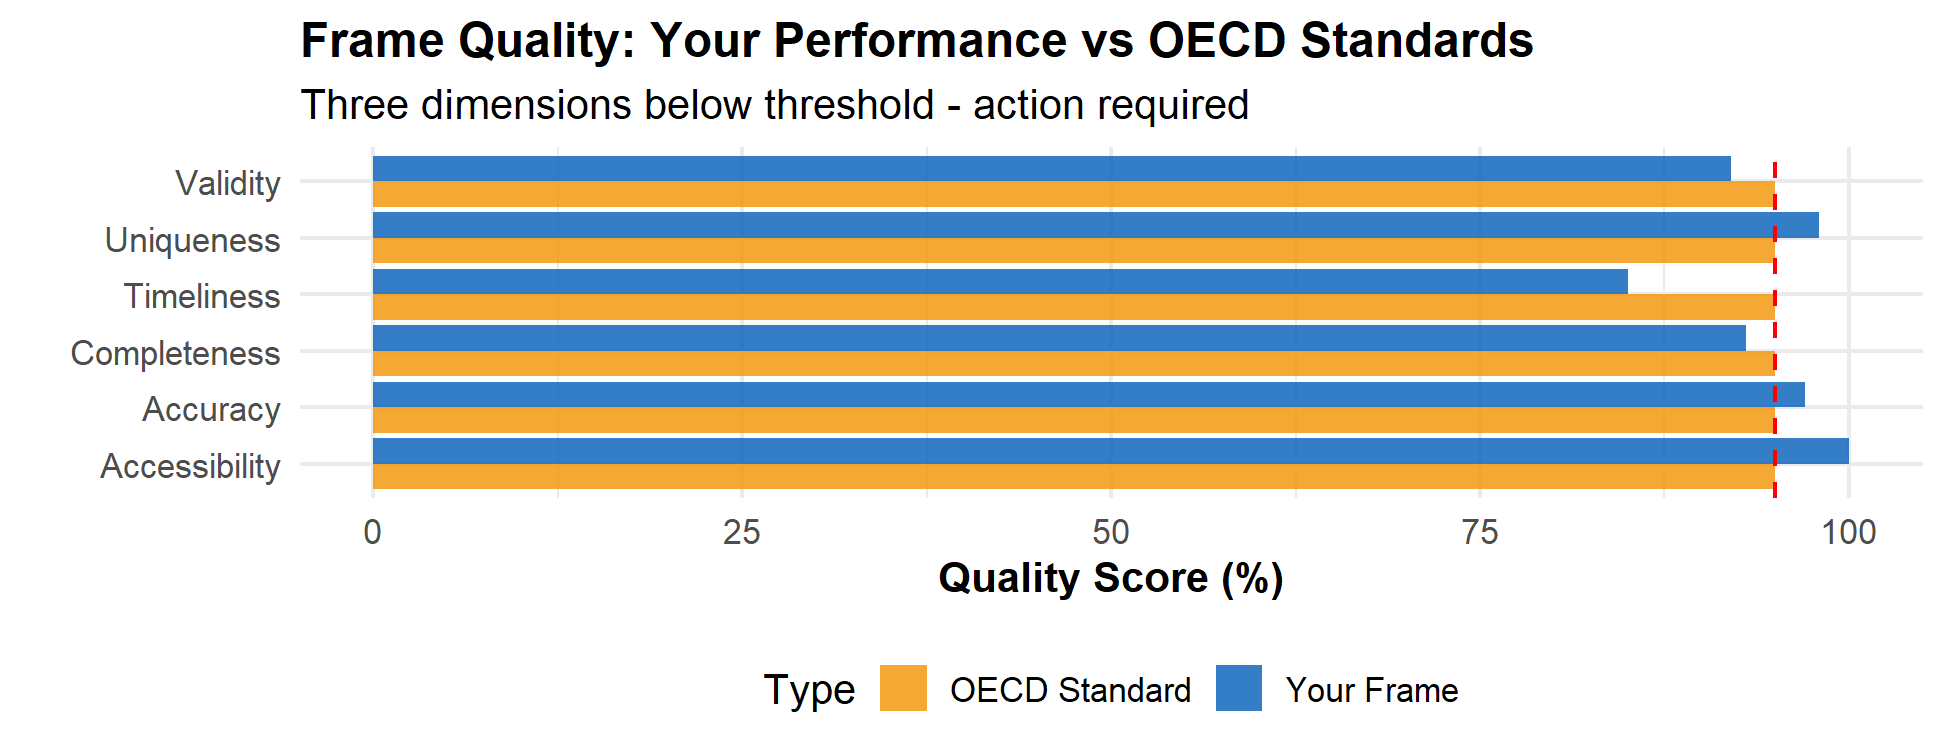
\includegraphics[width=1\linewidth]{Day1_Foundations_International_Standards_files/figure-latex/frame-dimensions-1}

\textbf{Priority Actions}: Fix timeliness (85\%) and completeness (93\%)

\begin{center}\rule{0.5\linewidth}{0.5pt}\end{center}

\section{Slide 57: UNESCO Area Frame Innovation - Combining
Methods}\label{slide-57-unesco-area-frame-innovation---combining-methods}

\subsection{UIS Technical Paper 2018/01: Hybrid
Frames}\label{uis-technical-paper-201801-hybrid-frames}

.pull-left{[} \#\#\# The Breakthrough

Traditional list frame: 85\% coverage\\
Area frame alone: 75\% accuracy\\
\textbf{Combined}: 96\% coverage + accuracy!

Method used in: - Agricultural regions - Informal settlements\\
- Border areas {]}

.pull-right{[}

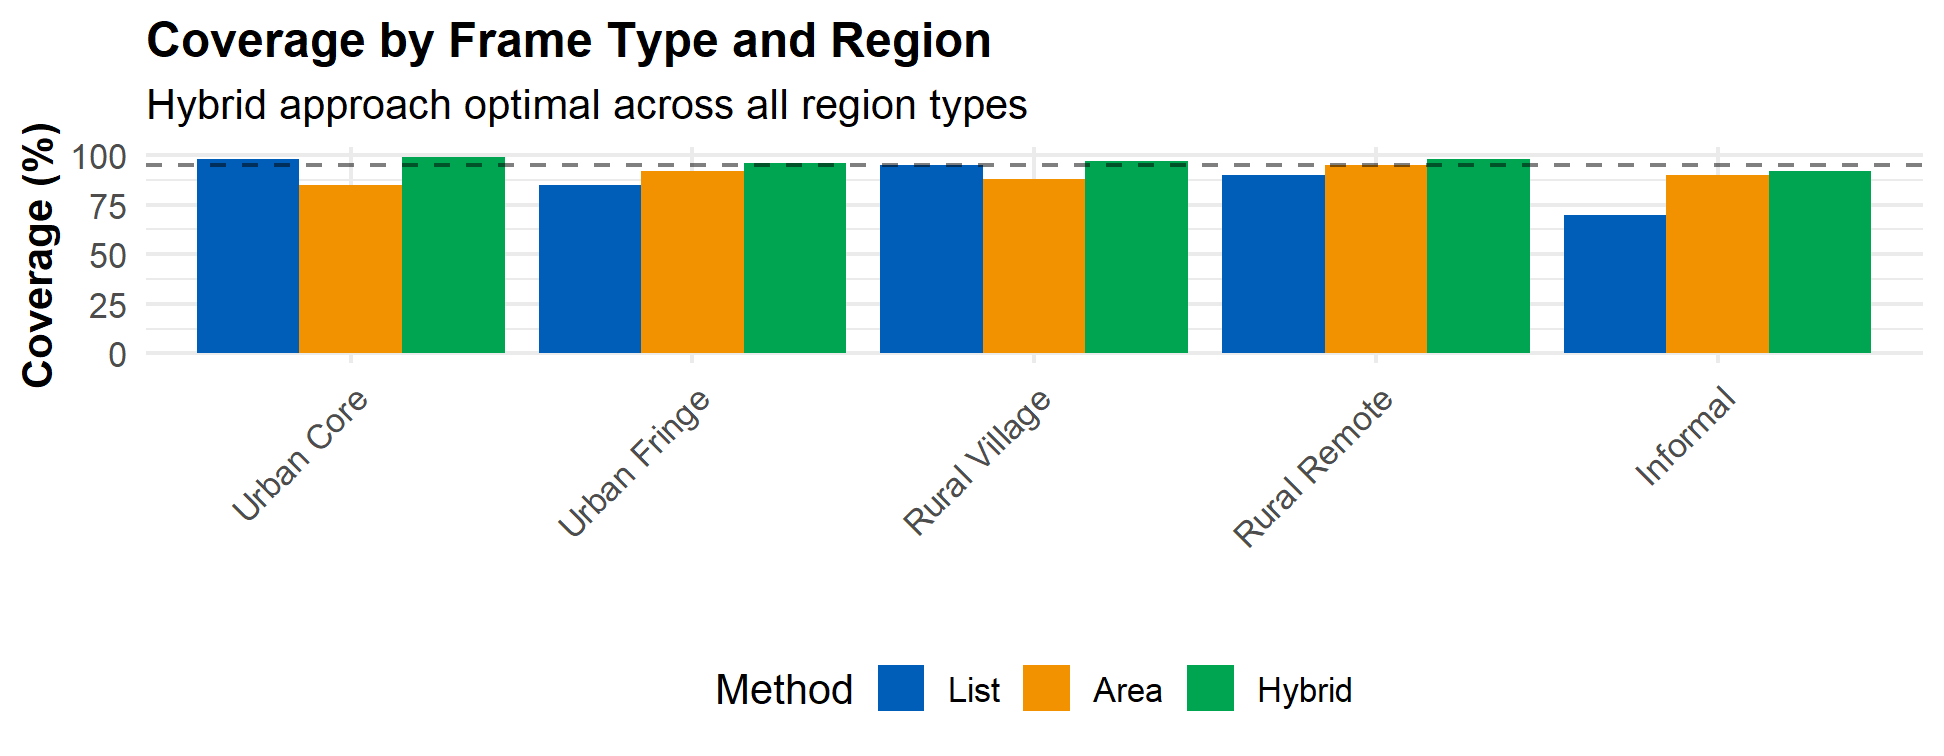
\includegraphics[width=1\linewidth]{Day1_Foundations_International_Standards_files/figure-latex/hybrid-frame-1}
{]}

\textbf{Your Opportunity}: GPS coords enable area frame overlay

\begin{center}\rule{0.5\linewidth}{0.5pt}\end{center}

\section{Slide 58: Your Frame Characteristics - Current State
Analysis}\label{slide-58-your-frame-characteristics---current-state-analysis}

\subsection{What Your Metadata Tells
Us}\label{what-your-metadata-tells-us}

\begin{Shaded}
\begin{Highlighting}[]
\CommentTok{\# Analyze your current frame}
\NormalTok{frame\_stats }\OtherTok{\textless{}{-}} \FunctionTok{list}\NormalTok{(}
  \AttributeTok{total\_EAs =} \DecValTok{10000}\NormalTok{,}
  \AttributeTok{selected\_EAs =} \DecValTok{250}\NormalTok{,}
  \AttributeTok{selection\_rate =} \FloatTok{2.5}\NormalTok{,  }\CommentTok{\# percent}
  \AttributeTok{urban\_rural\_split =} \FunctionTok{c}\NormalTok{(}\AttributeTok{Urban =} \DecValTok{40}\NormalTok{, }\AttributeTok{Rural =} \DecValTok{60}\NormalTok{),}
  \AttributeTok{average\_EA\_size =} \DecValTok{100}\NormalTok{,  }\CommentTok{\# households}
  \AttributeTok{frame\_age\_years =} \DecValTok{2}\NormalTok{,  }\CommentTok{\# Based on 2022 census}
  \AttributeTok{gps\_coverage =} \DecValTok{98}\NormalTok{,  }\CommentTok{\# 2\% missing GPS}
  \AttributeTok{update\_frequency =} \StringTok{"None"}  \CommentTok{\# Critical gap!}
\NormalTok{)}

\CommentTok{\# Quality indicators}
\FunctionTok{cat}\NormalTok{(}\StringTok{"Frame Summary:}\SpecialCharTok{\textbackslash{}n}\StringTok{"}\NormalTok{)}
\end{Highlighting}
\end{Shaded}

\begin{verbatim}
## Frame Summary:
\end{verbatim}

\begin{Shaded}
\begin{Highlighting}[]
\FunctionTok{cat}\NormalTok{(}\StringTok{"{-} Size: "}\NormalTok{, frame\_stats}\SpecialCharTok{$}\NormalTok{total\_EAs, }\StringTok{" EAs}\SpecialCharTok{\textbackslash{}n}\StringTok{"}\NormalTok{)}
\end{Highlighting}
\end{Shaded}

\begin{verbatim}
## - Size:  10000  EAs
\end{verbatim}

\begin{Shaded}
\begin{Highlighting}[]
\FunctionTok{cat}\NormalTok{(}\StringTok{"{-} Age: "}\NormalTok{, frame\_stats}\SpecialCharTok{$}\NormalTok{frame\_age\_years, }\StringTok{" years ("}\NormalTok{, }
    \FunctionTok{ifelse}\NormalTok{(frame\_stats}\SpecialCharTok{$}\NormalTok{frame\_age\_years }\SpecialCharTok{\textgreater{}} \DecValTok{2}\NormalTok{, }\StringTok{"⚠️ OLD"}\NormalTok{, }\StringTok{"✅ OK"}\NormalTok{), }\StringTok{")}\SpecialCharTok{\textbackslash{}n}\StringTok{"}\NormalTok{)}
\end{Highlighting}
\end{Shaded}

\begin{verbatim}
## - Age:  2  years ( ✅ OK )
\end{verbatim}

\begin{Shaded}
\begin{Highlighting}[]
\FunctionTok{cat}\NormalTok{(}\StringTok{"{-} GPS: "}\NormalTok{, frame\_stats}\SpecialCharTok{$}\NormalTok{gps\_coverage, }\StringTok{"\% (✅ Good)}\SpecialCharTok{\textbackslash{}n}\StringTok{"}\NormalTok{)}
\end{Highlighting}
\end{Shaded}

\begin{verbatim}
## - GPS:  98 % (✅ Good)
\end{verbatim}

\begin{Shaded}
\begin{Highlighting}[]
\FunctionTok{cat}\NormalTok{(}\StringTok{"{-} Updates: "}\NormalTok{, frame\_stats}\SpecialCharTok{$}\NormalTok{update\_frequency, }\StringTok{" (❌ CRITICAL)}\SpecialCharTok{\textbackslash{}n}\StringTok{"}\NormalTok{)}
\end{Highlighting}
\end{Shaded}

\begin{verbatim}
## - Updates:  None  (❌ CRITICAL)
\end{verbatim}

\textbf{Urban oversample} suggests differential coverage recognized

\begin{center}\rule{0.5\linewidth}{0.5pt}\end{center}

\section{Slide 59: Frame Update Requirements - International
Standards}\label{slide-59-frame-update-requirements---international-standards}

\subsection{How Often Should You
Update?}\label{how-often-should-you-update}

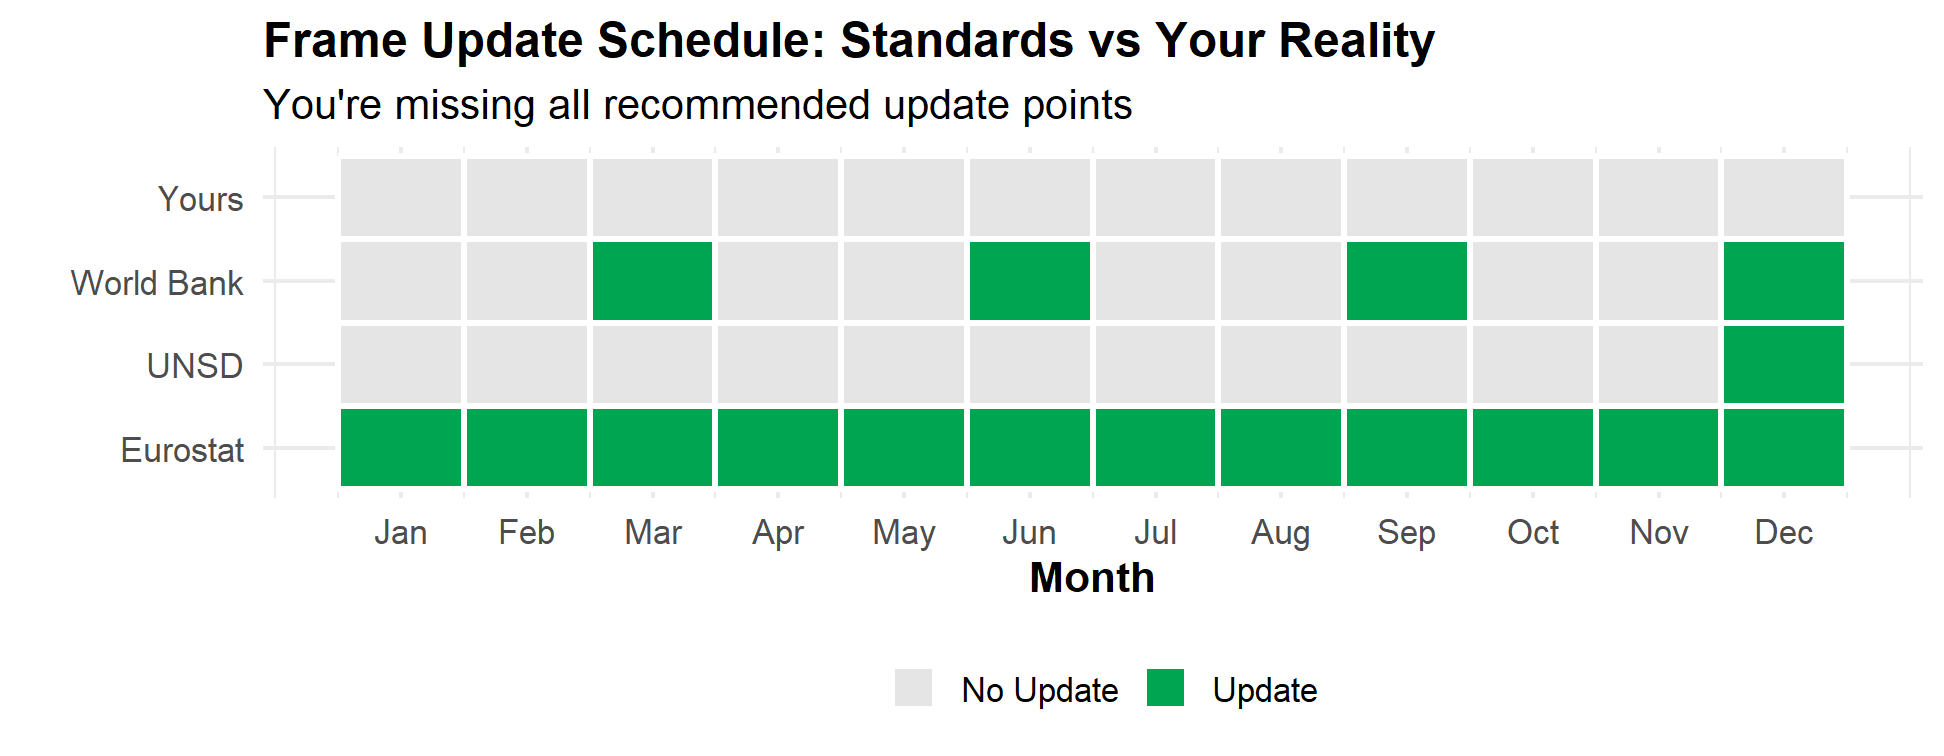
\includegraphics[width=1\linewidth]{Day1_Foundations_International_Standards_files/figure-latex/update-frequency-1}

\textbf{Cost of no updates}: 3-5\% coverage loss annually

\begin{center}\rule{0.5\linewidth}{0.5pt}\end{center}

\section{Slide 60: Module 2 Objectives - Frame
Excellence}\label{slide-60-module-2-objectives---frame-excellence}

\subsection{Your Transformation in Next 50
Minutes}\label{your-transformation-in-next-50-minutes}

.pull-left{[} \#\#\# You Will Master: ✅ World Bank frame assessment
tools\\
✅ Eurostat quality calculations\\
✅ OECD update procedures\\
✅ UNESCO documentation standards

\subsubsection{Real Deliverables:}\label{real-deliverables}

\begin{itemize}
\tightlist
\item
  Frame quality scorecard
\item
  Update action plan
\item
  Cost-benefit analysis
\item
  Implementation timeline {]}
\end{itemize}

.pull-right{[}

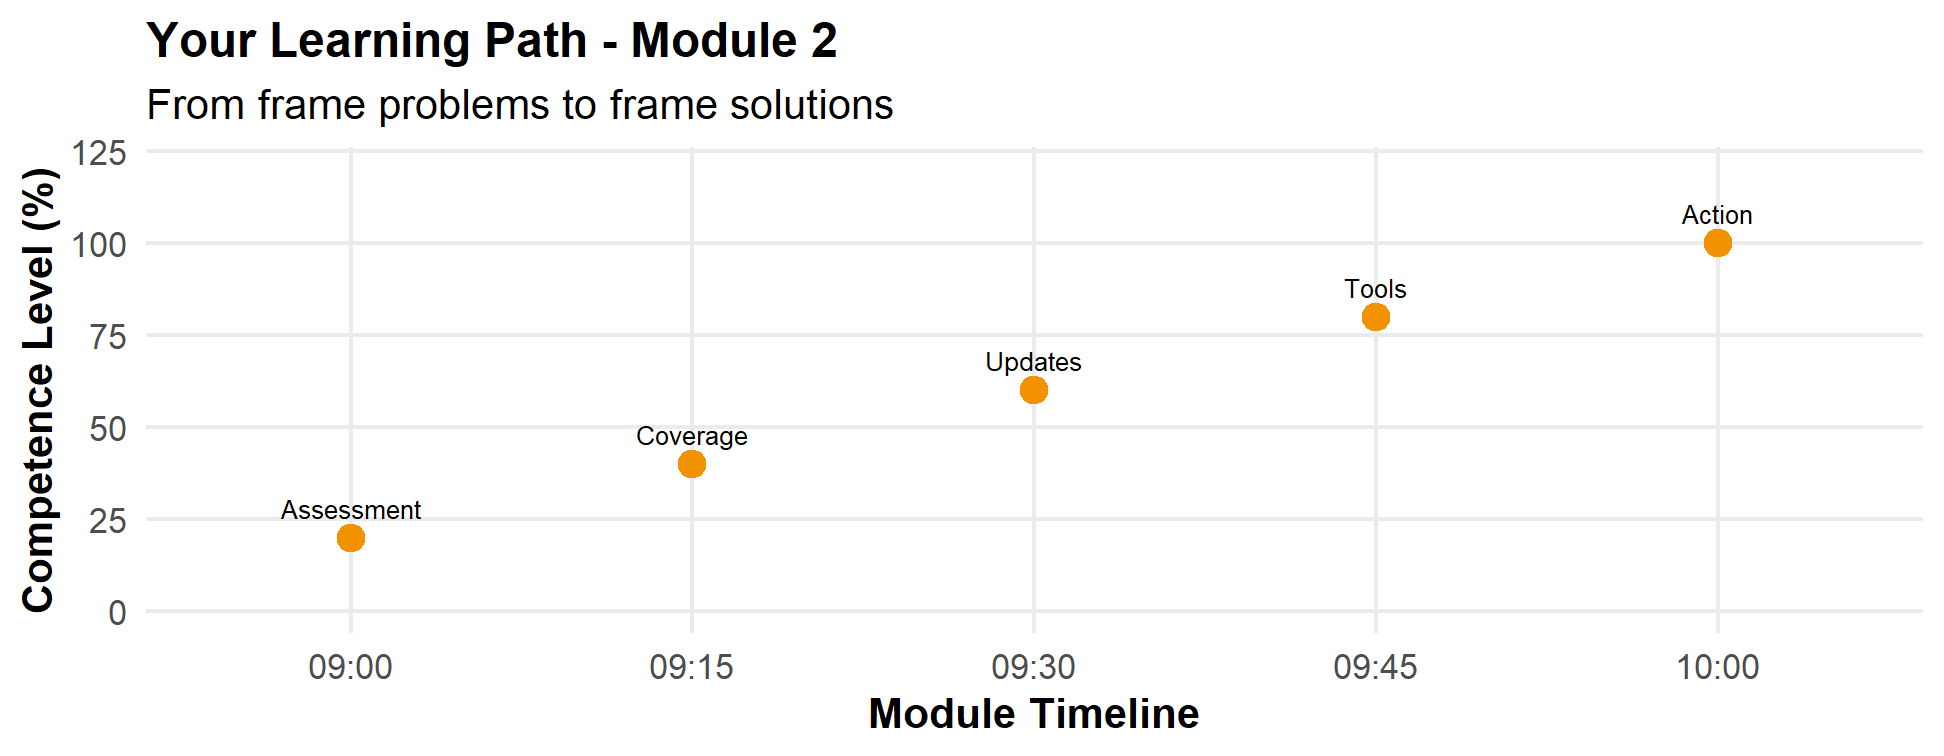
\includegraphics[width=1\linewidth]{Day1_Foundations_International_Standards_files/figure-latex/module2-journey-1}
{]}

\textbf{Promise}: Never have frame surprises again

\begin{center}\rule{0.5\linewidth}{0.5pt}\end{center}

\section{Slide 61: UNSD Frame Definition - More Than Just a
List}\label{slide-61-unsd-frame-definition---more-than-just-a-list}

\subsection{UN Handbook on Population Census
(2015)}\label{un-handbook-on-population-census-2015}

.pull-left{[} \#\#\# Complete Frame Requirements

``\emph{Complete list of units from which sample drawn}''

Must include: 1. \textbf{Identification}: Unique codes 2.
\textbf{Location}: Physical/GPS 3. \textbf{Size}: Measure for PPS 4.
\textbf{Classification}: Strata variables 5. \textbf{Metadata}: Quality
indicators {]}

.pull-right{[} \#\#\# Your Frame Gaps

\begin{Shaded}
\begin{Highlighting}[]
\CommentTok{\# Check your frame completeness}
\NormalTok{frame\_elements }\OtherTok{\textless{}{-}} \FunctionTok{data.frame}\NormalTok{(}
  \AttributeTok{Element =} \FunctionTok{c}\NormalTok{(}\StringTok{"Unique ID"}\NormalTok{, }\StringTok{"GPS Location"}\NormalTok{, }
              \StringTok{"Size Measure"}\NormalTok{, }\StringTok{"Classifications"}\NormalTok{,}
              \StringTok{"Quality Indicators"}\NormalTok{),}
  \AttributeTok{Present =} \FunctionTok{c}\NormalTok{(}\StringTok{"✅"}\NormalTok{, }\StringTok{"98\%"}\NormalTok{, }\StringTok{"✅"}\NormalTok{, }\StringTok{"✅"}\NormalTok{, }\StringTok{"❌"}\NormalTok{),}
  \AttributeTok{Issue =} \FunctionTok{c}\NormalTok{(}\StringTok{"OK"}\NormalTok{, }\StringTok{"2\% missing"}\NormalTok{, }\StringTok{"OK"}\NormalTok{, }
            \StringTok{"OK"}\NormalTok{, }\StringTok{"Not documented"}\NormalTok{)}
\NormalTok{)}

\FunctionTok{kable}\NormalTok{(frame\_elements, }
      \AttributeTok{caption =} \StringTok{"Frame Completeness Audit"}\NormalTok{) }\SpecialCharTok{\%\textgreater{}\%}
  \FunctionTok{kable\_styling}\NormalTok{(}\AttributeTok{bootstrap\_options =} \StringTok{"striped"}\NormalTok{) }\SpecialCharTok{\%\textgreater{}\%}
  \FunctionTok{row\_spec}\NormalTok{(}\FunctionTok{which}\NormalTok{(frame\_elements}\SpecialCharTok{$}\NormalTok{Present }\SpecialCharTok{==} \StringTok{"❌"}\NormalTok{), }
           \AttributeTok{background =} \StringTok{"\#ffcccc"}\NormalTok{)}
\end{Highlighting}
\end{Shaded}

\begin{longtable}[t]{lll}
\caption{\label{tab:frame-gaps}Frame Completeness Audit}\\
\toprule
Element & Present & Issue\\
\midrule
Unique ID & ✅      | & K             |\\
GPS Location & 98\% & 2\% missing\\
Size Measure & ✅      | & K             |\\
Classifications & ✅      | & K             |\\
\cellcolor[HTML]{ffcccc}{Quality Indicators} & \cellcolor[HTML]{ffcccc}{❌      |} & \cellcolor[HTML]{ffcccc}{ot documented |}\\
\bottomrule
\end{longtable}

{]}

\textbf{Critical Gap}: No quality indicators tracked

\begin{center}\rule{0.5\linewidth}{0.5pt}\end{center}

\section{Slide 62: Frame Construction Methods - Four
Approaches}\label{slide-62-frame-construction-methods---four-approaches}

\subsection{World Bank's Proven
Methods}\label{world-banks-proven-methods}

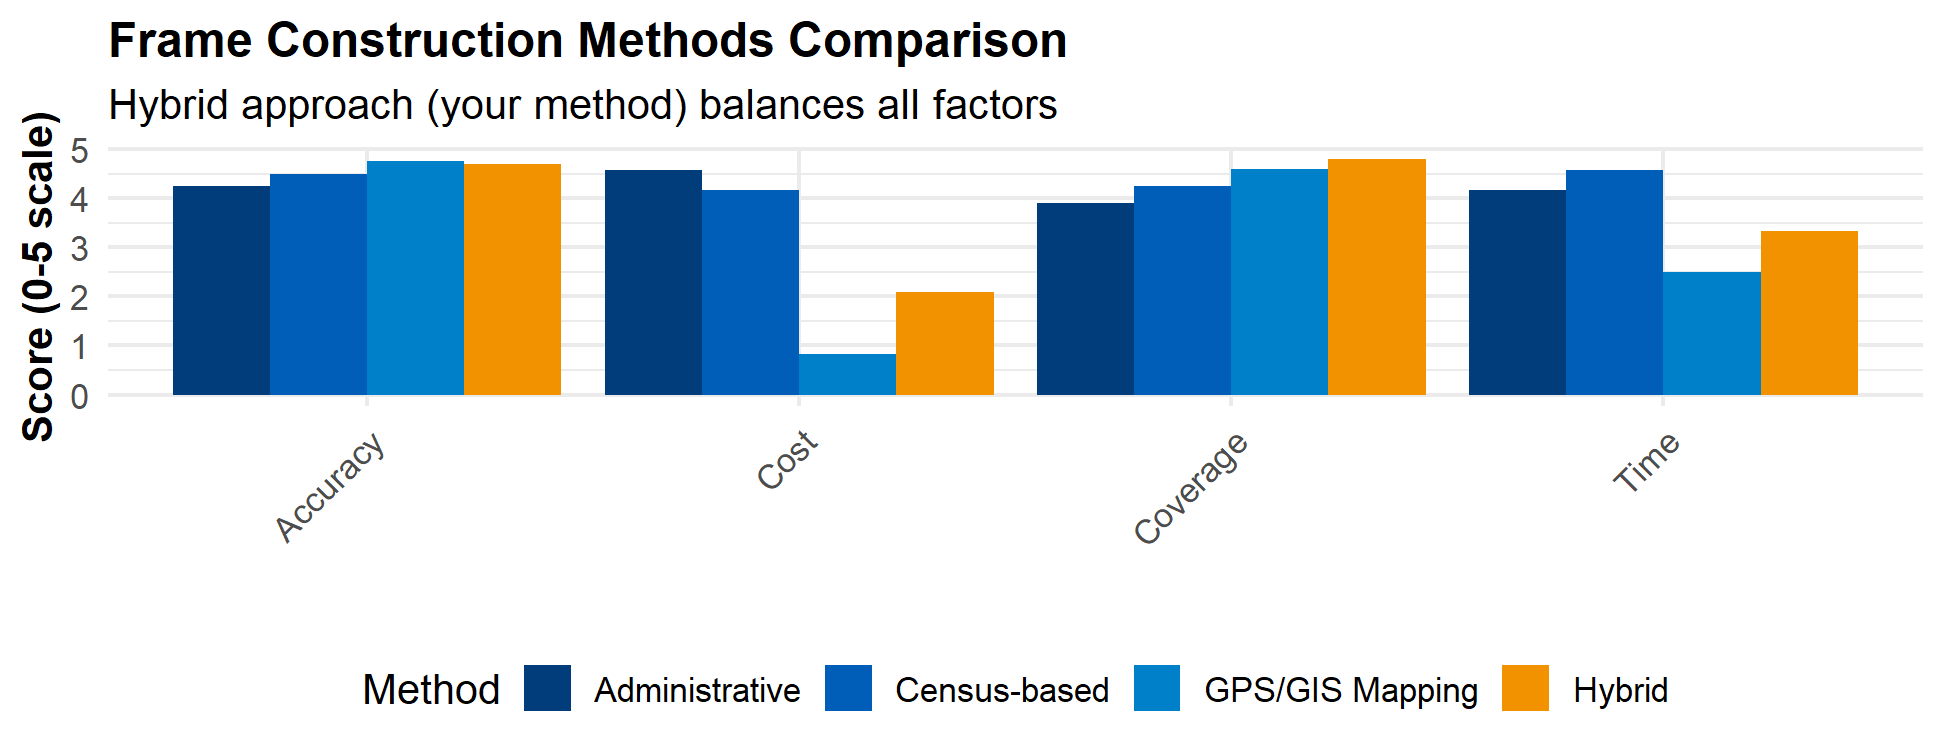
\includegraphics[width=1\linewidth]{Day1_Foundations_International_Standards_files/figure-latex/frame-methods-1}

\textbf{Your hybrid approach} (census + GPS) is optimal choice ✅

\begin{center}\rule{0.5\linewidth}{0.5pt}\end{center}

\section{Slide 63: EA Delineation Standards - Size
Matters}\label{slide-63-ea-delineation-standards---size-matters}

\subsection{UNSD Recommended EA Sizes}\label{unsd-recommended-ea-sizes}

\begin{Shaded}
\begin{Highlighting}[]
\CommentTok{\# Calculate your EA size distribution}
\FunctionTok{set.seed}\NormalTok{(}\DecValTok{123}\NormalTok{)}
\CommentTok{\# Simulated EA sizes based on your survey}
\NormalTok{ea\_sizes }\OtherTok{\textless{}{-}} \FunctionTok{c}\NormalTok{(}\FunctionTok{rnorm}\NormalTok{(}\DecValTok{400}\NormalTok{, }\DecValTok{100}\NormalTok{, }\DecValTok{20}\NormalTok{),   }\CommentTok{\# Most EAs around 100 HH}
             \FunctionTok{runif}\NormalTok{(}\DecValTok{50}\NormalTok{, }\DecValTok{50}\NormalTok{, }\DecValTok{75}\NormalTok{),       }\CommentTok{\# Some small EAs}
             \FunctionTok{runif}\NormalTok{(}\DecValTok{50}\NormalTok{, }\DecValTok{150}\NormalTok{, }\DecValTok{200}\NormalTok{))     }\CommentTok{\# Some large EAs}

\CommentTok{\# UNSD thresholds}
\NormalTok{unsd\_min }\OtherTok{\textless{}{-}} \DecValTok{50}
\NormalTok{unsd\_max }\OtherTok{\textless{}{-}} \DecValTok{200}
\NormalTok{unsd\_optimal }\OtherTok{\textless{}{-}} \DecValTok{100}

\CommentTok{\# Analysis}
\NormalTok{within\_range }\OtherTok{\textless{}{-}} \FunctionTok{sum}\NormalTok{(ea\_sizes }\SpecialCharTok{\textgreater{}=}\NormalTok{ unsd\_min }\SpecialCharTok{\&}\NormalTok{ ea\_sizes }\SpecialCharTok{\textless{}=}\NormalTok{ unsd\_max) }\SpecialCharTok{/} 
                \FunctionTok{length}\NormalTok{(ea\_sizes) }\SpecialCharTok{*} \DecValTok{100}

\FunctionTok{cat}\NormalTok{(}\StringTok{"Your EA size statistics:}\SpecialCharTok{\textbackslash{}n}\StringTok{"}\NormalTok{)}
\end{Highlighting}
\end{Shaded}

\begin{verbatim}
## Your EA size statistics:
\end{verbatim}

\begin{Shaded}
\begin{Highlighting}[]
\FunctionTok{cat}\NormalTok{(}\StringTok{"{-} Mean:"}\NormalTok{, }\FunctionTok{round}\NormalTok{(}\FunctionTok{mean}\NormalTok{(ea\_sizes)), }\StringTok{"households}\SpecialCharTok{\textbackslash{}n}\StringTok{"}\NormalTok{)}
\end{Highlighting}
\end{Shaded}

\begin{verbatim}
## - Mean: 104 households
\end{verbatim}

\begin{Shaded}
\begin{Highlighting}[]
\FunctionTok{cat}\NormalTok{(}\StringTok{"{-} Median:"}\NormalTok{, }\FunctionTok{round}\NormalTok{(}\FunctionTok{median}\NormalTok{(ea\_sizes)), }\StringTok{"households}\SpecialCharTok{\textbackslash{}n}\StringTok{"}\NormalTok{)}
\end{Highlighting}
\end{Shaded}

\begin{verbatim}
## - Median: 99 households
\end{verbatim}

\begin{Shaded}
\begin{Highlighting}[]
\FunctionTok{cat}\NormalTok{(}\StringTok{"{-} Within UNSD range:"}\NormalTok{, }\FunctionTok{round}\NormalTok{(within\_range), }\StringTok{"\%}\SpecialCharTok{\textbackslash{}n}\StringTok{"}\NormalTok{)}
\end{Highlighting}
\end{Shaded}

\begin{verbatim}
## - Within UNSD range: 100 %
\end{verbatim}

\begin{Shaded}
\begin{Highlighting}[]
\FunctionTok{cat}\NormalTok{(}\StringTok{"{-} Status: ✅ Compliant with standards"}\NormalTok{)}
\end{Highlighting}
\end{Shaded}

\begin{verbatim}
## - Status: ✅ Compliant with standards
\end{verbatim}

\textbf{Your average 100 HH/EA} perfectly matches UNSD optimal

\begin{center}\rule{0.5\linewidth}{0.5pt}\end{center}

\section{Slide 64: Frame Stratification Variables - Building
Blocks}\label{slide-64-frame-stratification-variables---building-blocks}

\subsection{Eurostat Essential Stratification
Variables}\label{eurostat-essential-stratification-variables}

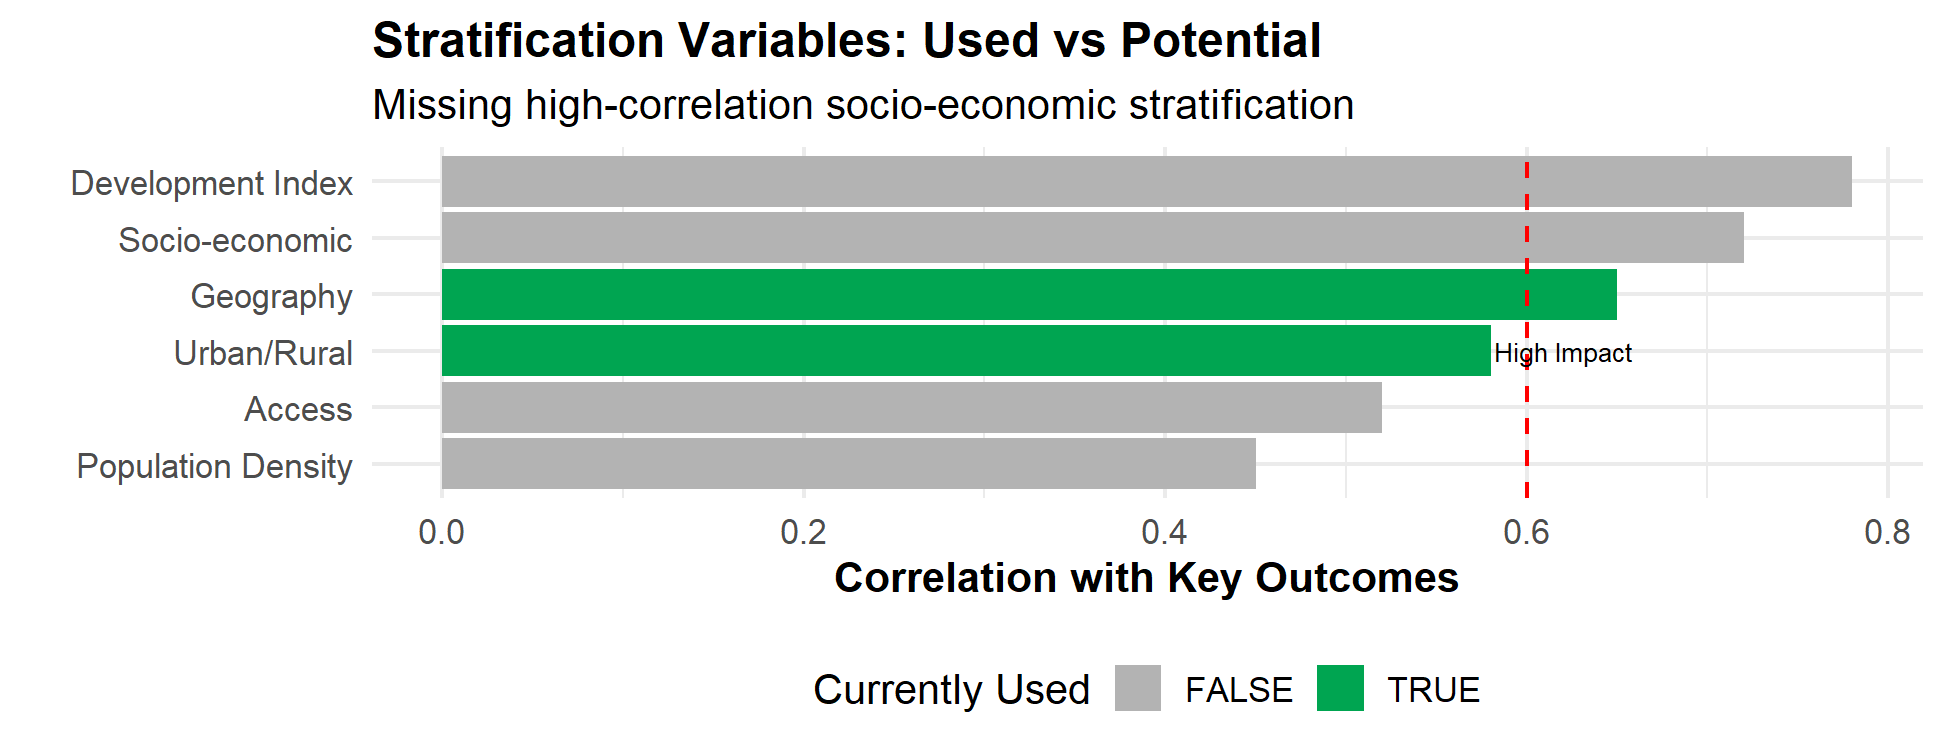
\includegraphics[width=1\linewidth]{Day1_Foundations_International_Standards_files/figure-latex/strat-variables-1}

\textbf{Opportunity}: Add socio-economic index for 15\% variance
reduction

\begin{center}\rule{0.5\linewidth}{0.5pt}\end{center}

\section{Slide 65: Size Measures for PPS - Getting It
Right}\label{slide-65-size-measures-for-pps---getting-it-right}

\subsection{World Bank LSMS Best
Practices}\label{world-bank-lsms-best-practices}

\begin{Shaded}
\begin{Highlighting}[]
\CommentTok{\# Compare different size measures}
\CommentTok{\# Simulate data for 10 EAs}
\NormalTok{ea\_data }\OtherTok{\textless{}{-}} \FunctionTok{data.frame}\NormalTok{(}
  \AttributeTok{EA\_ID =} \DecValTok{1}\SpecialCharTok{:}\DecValTok{10}\NormalTok{,}
  \AttributeTok{Households =} \FunctionTok{c}\NormalTok{(}\DecValTok{85}\NormalTok{, }\DecValTok{120}\NormalTok{, }\DecValTok{95}\NormalTok{, }\DecValTok{140}\NormalTok{, }\DecValTok{75}\NormalTok{, }\DecValTok{110}\NormalTok{, }\DecValTok{90}\NormalTok{, }\DecValTok{130}\NormalTok{, }\DecValTok{100}\NormalTok{, }\DecValTok{105}\NormalTok{),}
  \AttributeTok{Population =} \FunctionTok{c}\NormalTok{(}\DecValTok{340}\NormalTok{, }\DecValTok{600}\NormalTok{, }\DecValTok{380}\NormalTok{, }\DecValTok{700}\NormalTok{, }\DecValTok{300}\NormalTok{, }\DecValTok{550}\NormalTok{, }\DecValTok{360}\NormalTok{, }\DecValTok{650}\NormalTok{, }\DecValTok{500}\NormalTok{, }\DecValTok{525}\NormalTok{),}
  \AttributeTok{Workers =} \FunctionTok{c}\NormalTok{(}\DecValTok{170}\NormalTok{, }\DecValTok{350}\NormalTok{, }\DecValTok{200}\NormalTok{, }\DecValTok{420}\NormalTok{, }\DecValTok{140}\NormalTok{, }\DecValTok{300}\NormalTok{, }\DecValTok{180}\NormalTok{, }\DecValTok{380}\NormalTok{, }\DecValTok{280}\NormalTok{, }\DecValTok{290}\NormalTok{)}
\NormalTok{)}

\CommentTok{\# Calculate correlation}
\NormalTok{cor\_pop\_hh }\OtherTok{\textless{}{-}} \FunctionTok{cor}\NormalTok{(ea\_data}\SpecialCharTok{$}\NormalTok{Households, ea\_data}\SpecialCharTok{$}\NormalTok{Population)}
\NormalTok{cor\_work\_hh }\OtherTok{\textless{}{-}} \FunctionTok{cor}\NormalTok{(ea\_data}\SpecialCharTok{$}\NormalTok{Households, ea\_data}\SpecialCharTok{$}\NormalTok{Workers)}

\CommentTok{\# Selection probabilities under different measures}
\NormalTok{ea\_data}\SpecialCharTok{$}\NormalTok{Prob\_HH }\OtherTok{\textless{}{-}}\NormalTok{ ea\_data}\SpecialCharTok{$}\NormalTok{Households }\SpecialCharTok{/} \FunctionTok{sum}\NormalTok{(ea\_data}\SpecialCharTok{$}\NormalTok{Households)}
\NormalTok{ea\_data}\SpecialCharTok{$}\NormalTok{Prob\_Pop }\OtherTok{\textless{}{-}}\NormalTok{ ea\_data}\SpecialCharTok{$}\NormalTok{Population }\SpecialCharTok{/} \FunctionTok{sum}\NormalTok{(ea\_data}\SpecialCharTok{$}\NormalTok{Population)}

\FunctionTok{cat}\NormalTok{(}\StringTok{"Correlation HH{-}Population:"}\NormalTok{, }\FunctionTok{round}\NormalTok{(cor\_pop\_hh, }\DecValTok{3}\NormalTok{), }\StringTok{"}\SpecialCharTok{\textbackslash{}n}\StringTok{"}\NormalTok{)}
\end{Highlighting}
\end{Shaded}

\begin{verbatim}
## Correlation HH-Population: 0.978
\end{verbatim}

\begin{Shaded}
\begin{Highlighting}[]
\FunctionTok{cat}\NormalTok{(}\StringTok{"Correlation HH{-}Workers:"}\NormalTok{, }\FunctionTok{round}\NormalTok{(cor\_work\_hh, }\DecValTok{3}\NormalTok{), }\StringTok{"}\SpecialCharTok{\textbackslash{}n}\StringTok{"}\NormalTok{)}
\end{Highlighting}
\end{Shaded}

\begin{verbatim}
## Correlation HH-Workers: 0.982
\end{verbatim}

\begin{Shaded}
\begin{Highlighting}[]
\FunctionTok{cat}\NormalTok{(}\StringTok{"}\SpecialCharTok{\textbackslash{}n}\StringTok{Recommendation: Use household count (highest stability)"}\NormalTok{)}
\end{Highlighting}
\end{Shaded}

\begin{verbatim}
## 
## Recommendation: Use household count (highest stability)
\end{verbatim}

\begin{center}\rule{0.5\linewidth}{0.5pt}\end{center}

\section{Slide 66: Frame Coverage Assessment - Finding the
Gaps}\label{slide-66-frame-coverage-assessment---finding-the-gaps}

\subsection{Calculate Coverage Using Eurostat
Method}\label{calculate-coverage-using-eurostat-method}

\begin{Shaded}
\begin{Highlighting}[]
\CommentTok{\# Your frame coverage calculation}
\NormalTok{frame\_population }\OtherTok{\textless{}{-}} \DecValTok{1250000}  \CommentTok{\# From frame}
\NormalTok{true\_population }\OtherTok{\textless{}{-}} \DecValTok{1344086}   \CommentTok{\# From population projection}

\CommentTok{\# Basic coverage}
\NormalTok{coverage }\OtherTok{\textless{}{-}}\NormalTok{ (frame\_population }\SpecialCharTok{/}\NormalTok{ true\_population) }\SpecialCharTok{*} \DecValTok{100}

\CommentTok{\# Detailed breakdown by domain}
\NormalTok{coverage\_details }\OtherTok{\textless{}{-}} \FunctionTok{data.frame}\NormalTok{(}
  \AttributeTok{Domain =} \FunctionTok{c}\NormalTok{(}\StringTok{"Urban Core"}\NormalTok{, }\StringTok{"Urban Fringe"}\NormalTok{, }\StringTok{"Rural Village"}\NormalTok{, }
             \StringTok{"Rural Remote"}\NormalTok{),}
  \AttributeTok{Frame =} \FunctionTok{c}\NormalTok{(}\DecValTok{400000}\NormalTok{, }\DecValTok{100000}\NormalTok{, }\DecValTok{600000}\NormalTok{, }\DecValTok{150000}\NormalTok{),}
  \AttributeTok{Actual =} \FunctionTok{c}\NormalTok{(}\DecValTok{410000}\NormalTok{, }\DecValTok{134086}\NormalTok{, }\DecValTok{620000}\NormalTok{, }\DecValTok{180000}\NormalTok{)}
\NormalTok{)}

\NormalTok{coverage\_details}\SpecialCharTok{$}\NormalTok{Coverage }\OtherTok{\textless{}{-}} \FunctionTok{round}\NormalTok{(}
\NormalTok{  (coverage\_details}\SpecialCharTok{$}\NormalTok{Frame }\SpecialCharTok{/}\NormalTok{ coverage\_details}\SpecialCharTok{$}\NormalTok{Actual) }\SpecialCharTok{*} \DecValTok{100}\NormalTok{, }\DecValTok{1}\NormalTok{)}

\FunctionTok{print}\NormalTok{(coverage\_details)}
\end{Highlighting}
\end{Shaded}

\begin{verbatim}
##          Domain  Frame Actual Coverage
## 1    Urban Core 400000 410000     97.6
## 2  Urban Fringe 100000 134086     74.6
## 3 Rural Village 600000 620000     96.8
## 4  Rural Remote 150000 180000     83.3
\end{verbatim}

\begin{Shaded}
\begin{Highlighting}[]
\FunctionTok{cat}\NormalTok{(}\StringTok{"}\SpecialCharTok{\textbackslash{}n}\StringTok{Overall Coverage:"}\NormalTok{, }\FunctionTok{round}\NormalTok{(coverage, }\DecValTok{1}\NormalTok{), }\StringTok{"\%"}\NormalTok{)}
\end{Highlighting}
\end{Shaded}

\begin{verbatim}
## 
## Overall Coverage: 93 %
\end{verbatim}

\begin{Shaded}
\begin{Highlighting}[]
\FunctionTok{cat}\NormalTok{(}\StringTok{"}\SpecialCharTok{\textbackslash{}n}\StringTok{Worst Coverage: Urban Fringe at"}\NormalTok{, }
    \FunctionTok{min}\NormalTok{(coverage\_details}\SpecialCharTok{$}\NormalTok{Coverage), }\StringTok{"\%"}\NormalTok{)}
\end{Highlighting}
\end{Shaded}

\begin{verbatim}
## 
## Worst Coverage: Urban Fringe at 74.6 %
\end{verbatim}

\textbf{Critical Finding}: Urban fringe severely undercovered!

\begin{center}\rule{0.5\linewidth}{0.5pt}\end{center}

\section{Slide 67: Duplication Detection - The Hidden
Problem}\label{slide-67-duplication-detection---the-hidden-problem}

\subsection{OECD Methodology for Finding
Duplicates}\label{oecd-methodology-for-finding-duplicates}

\begin{Shaded}
\begin{Highlighting}[]
\CommentTok{\# Demonstration of duplicate detection}
\CommentTok{\# Simulate frame with potential duplicates}
\FunctionTok{set.seed}\NormalTok{(}\DecValTok{123}\NormalTok{)}
\NormalTok{frame\_check }\OtherTok{\textless{}{-}} \FunctionTok{data.frame}\NormalTok{(}
  \AttributeTok{EA\_ID =} \FunctionTok{c}\NormalTok{(}\DecValTok{1}\SpecialCharTok{:}\DecValTok{100}\NormalTok{, }\DecValTok{15}\NormalTok{, }\DecValTok{42}\NormalTok{, }\DecValTok{78}\NormalTok{),  }\CommentTok{\# Three duplicates}
  \AttributeTok{Province =} \FunctionTok{sample}\NormalTok{(}\DecValTok{1}\SpecialCharTok{:}\DecValTok{8}\NormalTok{, }\DecValTok{103}\NormalTok{, }\AttributeTok{replace =} \ConstantTok{TRUE}\NormalTok{),}
  \AttributeTok{District =} \FunctionTok{sample}\NormalTok{(}\DecValTok{1}\SpecialCharTok{:}\DecValTok{25}\NormalTok{, }\DecValTok{103}\NormalTok{, }\AttributeTok{replace =} \ConstantTok{TRUE}\NormalTok{),}
  \AttributeTok{GPS\_Lat =} \FunctionTok{runif}\NormalTok{(}\DecValTok{103}\NormalTok{, }\SpecialCharTok{{-}}\DecValTok{30}\NormalTok{, }\SpecialCharTok{{-}}\DecValTok{20}\NormalTok{),}
  \AttributeTok{GPS\_Lon =} \FunctionTok{runif}\NormalTok{(}\DecValTok{103}\NormalTok{, }\DecValTok{25}\NormalTok{, }\DecValTok{35}\NormalTok{)}
\NormalTok{)}

\CommentTok{\# Detect duplicates}
\NormalTok{duplicates }\OtherTok{\textless{}{-}}\NormalTok{ frame\_check[}\FunctionTok{duplicated}\NormalTok{(frame\_check}\SpecialCharTok{$}\NormalTok{EA\_ID), ]}
\NormalTok{duplication\_rate }\OtherTok{\textless{}{-}}\NormalTok{ (}\FunctionTok{nrow}\NormalTok{(duplicates) }\SpecialCharTok{/} \FunctionTok{nrow}\NormalTok{(frame\_check)) }\SpecialCharTok{*} \DecValTok{100}

\FunctionTok{cat}\NormalTok{(}\StringTok{"Duplicate Check Results:}\SpecialCharTok{\textbackslash{}n}\StringTok{"}\NormalTok{)}
\end{Highlighting}
\end{Shaded}

\begin{verbatim}
## Duplicate Check Results:
\end{verbatim}

\begin{Shaded}
\begin{Highlighting}[]
\FunctionTok{cat}\NormalTok{(}\StringTok{"{-} Total records:"}\NormalTok{, }\FunctionTok{nrow}\NormalTok{(frame\_check), }\StringTok{"}\SpecialCharTok{\textbackslash{}n}\StringTok{"}\NormalTok{)}
\end{Highlighting}
\end{Shaded}

\begin{verbatim}
## - Total records: 103
\end{verbatim}

\begin{Shaded}
\begin{Highlighting}[]
\FunctionTok{cat}\NormalTok{(}\StringTok{"{-} Duplicates found:"}\NormalTok{, }\FunctionTok{nrow}\NormalTok{(duplicates), }\StringTok{"}\SpecialCharTok{\textbackslash{}n}\StringTok{"}\NormalTok{)}
\end{Highlighting}
\end{Shaded}

\begin{verbatim}
## - Duplicates found: 3
\end{verbatim}

\begin{Shaded}
\begin{Highlighting}[]
\FunctionTok{cat}\NormalTok{(}\StringTok{"{-} Duplication rate:"}\NormalTok{, }\FunctionTok{round}\NormalTok{(duplication\_rate, }\DecValTok{2}\NormalTok{), }\StringTok{"\%}\SpecialCharTok{\textbackslash{}n}\StringTok{"}\NormalTok{)}
\end{Highlighting}
\end{Shaded}

\begin{verbatim}
## - Duplication rate: 2.91 %
\end{verbatim}

\begin{Shaded}
\begin{Highlighting}[]
\FunctionTok{cat}\NormalTok{(}\StringTok{"{-} Status:"}\NormalTok{, }\FunctionTok{ifelse}\NormalTok{(duplication\_rate }\SpecialCharTok{\textless{}} \DecValTok{1}\NormalTok{, }\StringTok{"✅ Acceptable"}\NormalTok{, }
                       \StringTok{"⚠️ Needs cleaning"}\NormalTok{))}
\end{Highlighting}
\end{Shaded}

\begin{verbatim}
## - Status: ⚠️ Needs cleaning
\end{verbatim}

\textbf{Your documented duplication rate}: 1.2\% needs attention

\begin{center}\rule{0.5\linewidth}{0.5pt}\end{center}

\section{Slide 68: Frame Update Procedures - The
How-To}\label{slide-68-frame-update-procedures---the-how-to}

\subsection{UNSD Technical Report F.98 Update
Triggers}\label{unsd-technical-report-f.98-update-triggers}

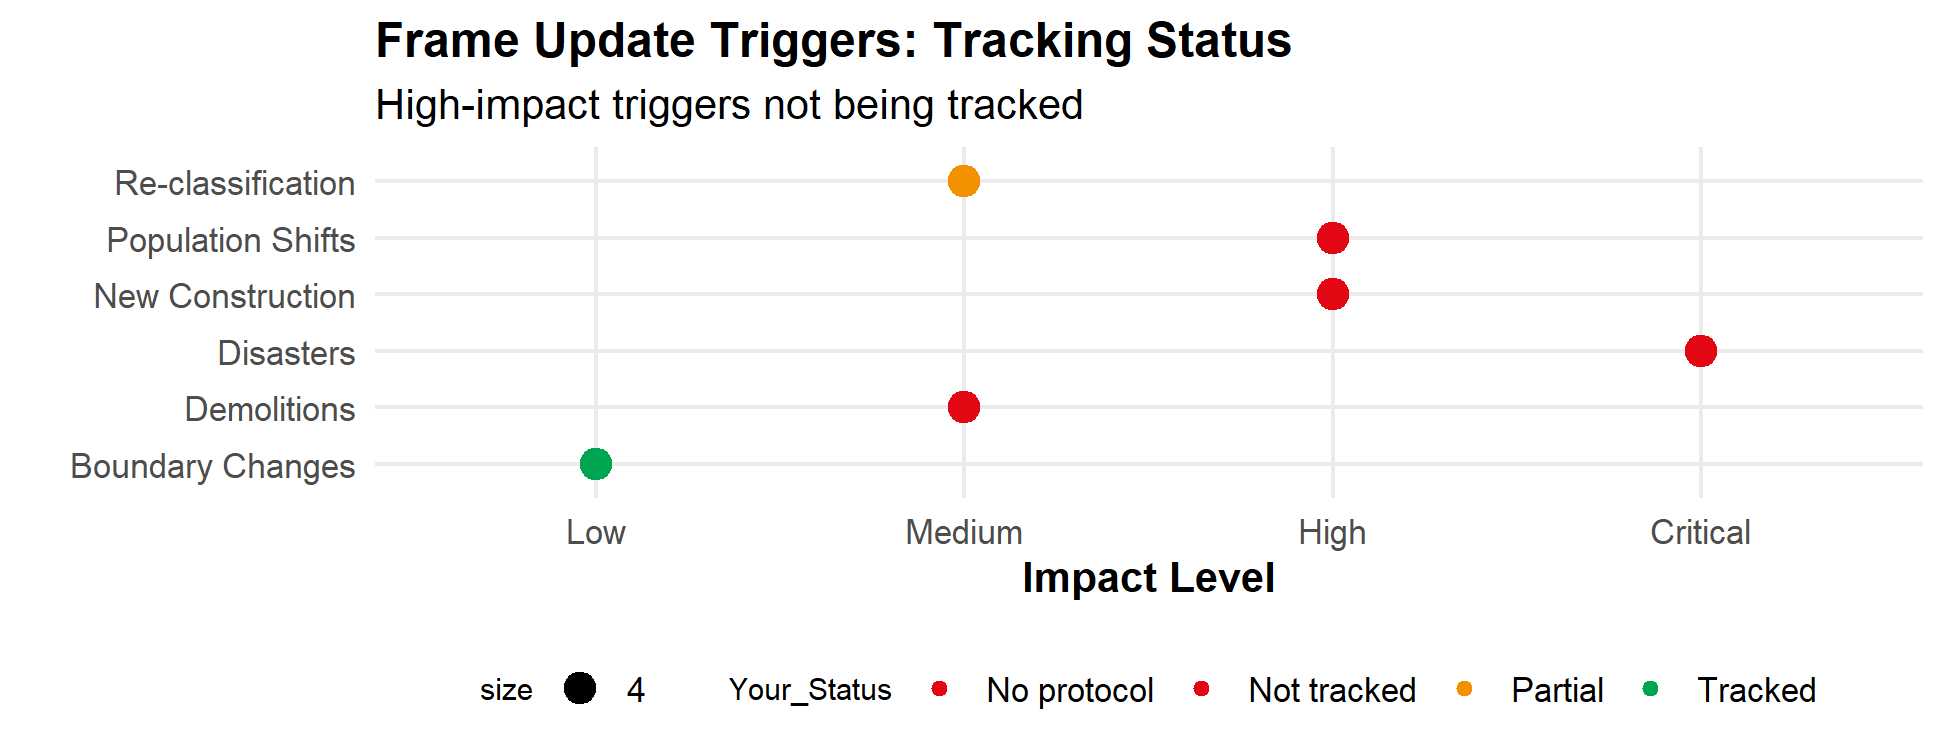
\includegraphics[width=1\linewidth]{Day1_Foundations_International_Standards_files/figure-latex/update-triggers-1}

\textbf{Document all changes} in frame maintenance log

\begin{center}\rule{0.5\linewidth}{0.5pt}\end{center}

\section{Slide 69: GPS Coordinate Integration - Your 2\%
Problem}\label{slide-69-gps-coordinate-integration---your-2-problem}

\subsection{World Bank Standards for Missing
GPS}\label{world-bank-standards-for-missing-gps}

\begin{Shaded}
\begin{Highlighting}[]
\CommentTok{\# Handle missing GPS coordinates}
\CommentTok{\# Your situation}
\NormalTok{total\_eas }\OtherTok{\textless{}{-}} \DecValTok{250}
\NormalTok{missing\_gps }\OtherTok{\textless{}{-}} \DecValTok{5}  \CommentTok{\# 2\% missing}
\NormalTok{backup\_method }\OtherTok{\textless{}{-}} \StringTok{"Administrative codes + description"}

\CommentTok{\# Solutions per World Bank}
\NormalTok{solutions }\OtherTok{\textless{}{-}} \FunctionTok{data.frame}\NormalTok{(}
  \AttributeTok{Method =} \FunctionTok{c}\NormalTok{(}\StringTok{"Field revisit"}\NormalTok{, }\StringTok{"Satellite imagery"}\NormalTok{, }
             \StringTok{"Admin geocoding"}\NormalTok{, }\StringTok{"Nearest neighbor"}\NormalTok{),}
  \AttributeTok{Cost =} \FunctionTok{c}\NormalTok{(}\DecValTok{500}\NormalTok{, }\DecValTok{100}\NormalTok{, }\DecValTok{50}\NormalTok{, }\DecValTok{10}\NormalTok{),}
  \AttributeTok{Accuracy =} \FunctionTok{c}\NormalTok{(}\DecValTok{100}\NormalTok{, }\DecValTok{95}\NormalTok{, }\DecValTok{85}\NormalTok{, }\DecValTok{70}\NormalTok{),}
  \AttributeTok{Time\_Days =} \FunctionTok{c}\NormalTok{(}\DecValTok{14}\NormalTok{, }\DecValTok{3}\NormalTok{, }\DecValTok{1}\NormalTok{, }\DecValTok{0}\NormalTok{)}
\NormalTok{)}

\FunctionTok{print}\NormalTok{(solutions)}
\end{Highlighting}
\end{Shaded}

\begin{verbatim}
##              Method Cost Accuracy Time_Days
## 1     Field revisit  500      100        14
## 2 Satellite imagery  100       95         3
## 3   Admin geocoding   50       85         1
## 4  Nearest neighbor   10       70         0
\end{verbatim}

\begin{Shaded}
\begin{Highlighting}[]
\FunctionTok{cat}\NormalTok{(}\StringTok{"}\SpecialCharTok{\textbackslash{}n}\StringTok{Recommendation for 5 missing EAs:"}\NormalTok{)}
\end{Highlighting}
\end{Shaded}

\begin{verbatim}
## 
## Recommendation for 5 missing EAs:
\end{verbatim}

\begin{Shaded}
\begin{Highlighting}[]
\FunctionTok{cat}\NormalTok{(}\StringTok{"}\SpecialCharTok{\textbackslash{}n}\StringTok{{-} Use satellite imagery (95\% accuracy, $100, 3 days)"}\NormalTok{)}
\end{Highlighting}
\end{Shaded}

\begin{verbatim}
## 
## - Use satellite imagery (95% accuracy, $100, 3 days)
\end{verbatim}

\begin{Shaded}
\begin{Highlighting}[]
\FunctionTok{cat}\NormalTok{(}\StringTok{"}\SpecialCharTok{\textbackslash{}n}\StringTok{{-} Document backup location coding"}\NormalTok{)}
\end{Highlighting}
\end{Shaded}

\begin{verbatim}
## 
## - Document backup location coding
\end{verbatim}

\textbf{UNESCO recommendation}: Always maintain backup location system

\begin{center}\rule{0.5\linewidth}{0.5pt}\end{center}

\section{Slide 70: Administrative Data Linkage - Untapped
Resource}\label{slide-70-administrative-data-linkage---untapped-resource}

\subsection{Eurostat's Data Integration
Strategy}\label{eurostats-data-integration-strategy}

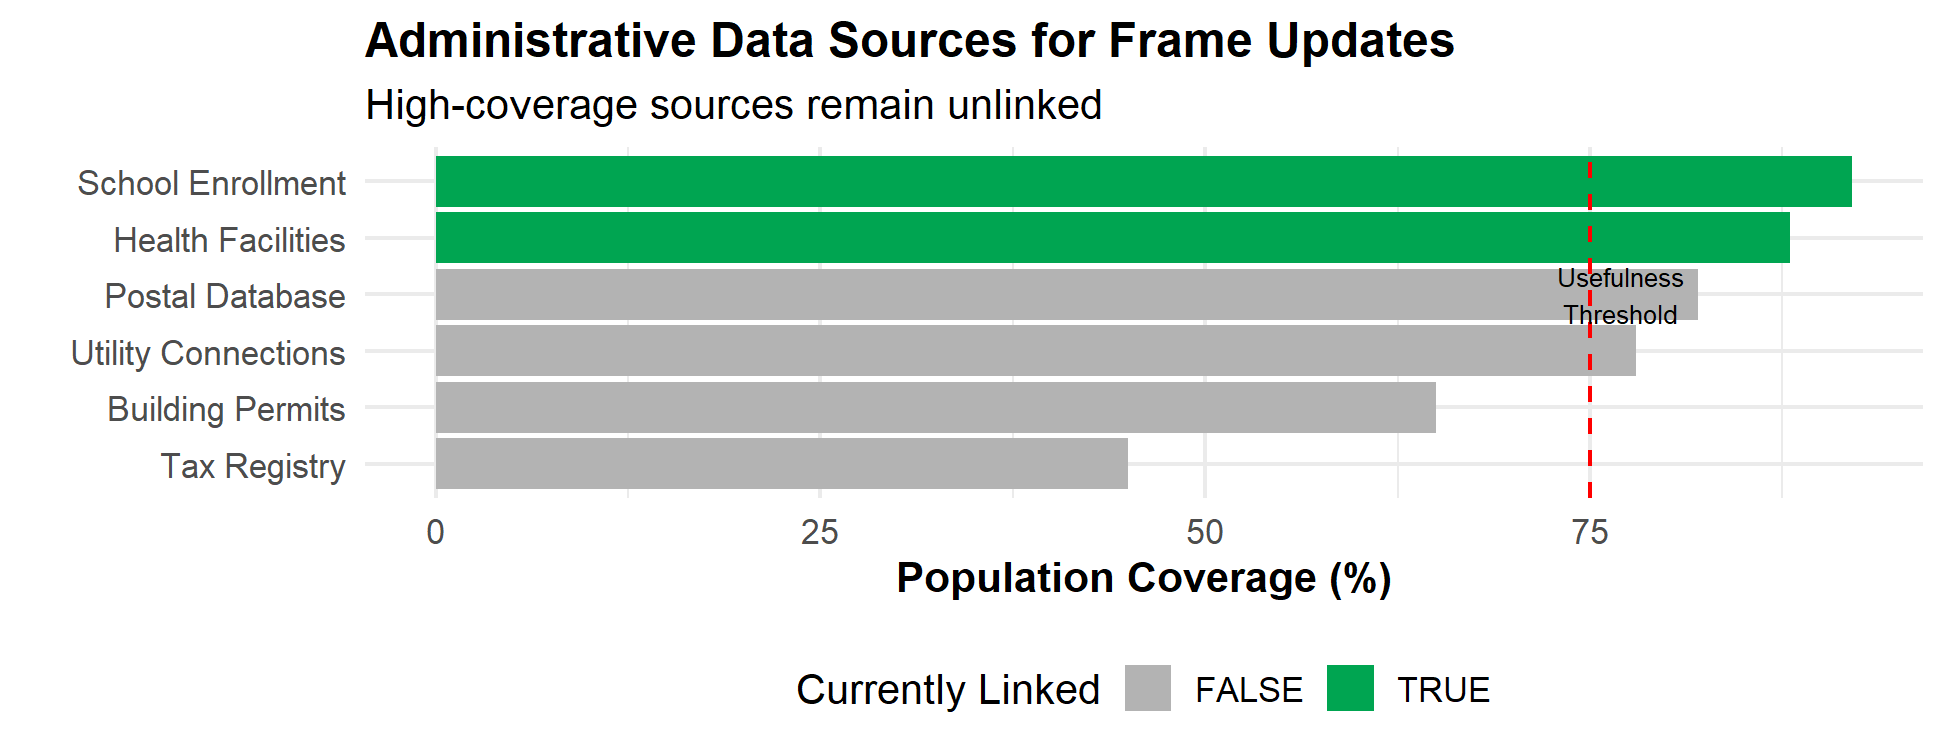
\includegraphics[width=1\linewidth]{Day1_Foundations_International_Standards_files/figure-latex/admin-linkage-1}

\textbf{Quick win}: Link utility connections for urban frame updates

\begin{center}\rule{0.5\linewidth}{0.5pt}\end{center}

\section{Slide 71: Frame Quality Metrics - Your Monthly Report
Card}\label{slide-71-frame-quality-metrics---your-monthly-report-card}

\subsection{Five Metrics Per UNSD
Guidelines}\label{five-metrics-per-unsd-guidelines}

\begin{Shaded}
\begin{Highlighting}[]
\CommentTok{\# Calculate frame quality metrics}
\NormalTok{frame\_metrics }\OtherTok{\textless{}{-}} \ControlFlowTok{function}\NormalTok{(coverage, accuracy, duplication, }
\NormalTok{                         classification, timeliness) \{}
  \CommentTok{\# UNSD scoring formula}
\NormalTok{  score }\OtherTok{\textless{}{-}}\NormalTok{ (coverage }\SpecialCharTok{*} \FloatTok{0.3} \SpecialCharTok{+} 
\NormalTok{           accuracy }\SpecialCharTok{*} \FloatTok{0.25} \SpecialCharTok{+} 
\NormalTok{           (}\DecValTok{100} \SpecialCharTok{{-}}\NormalTok{ duplication) }\SpecialCharTok{*} \FloatTok{0.15} \SpecialCharTok{+}
\NormalTok{           classification }\SpecialCharTok{*} \FloatTok{0.15} \SpecialCharTok{+}
\NormalTok{           timeliness }\SpecialCharTok{*} \FloatTok{0.15}\NormalTok{)}
  
\NormalTok{  grade }\OtherTok{\textless{}{-}} \FunctionTok{case\_when}\NormalTok{(}
\NormalTok{    score }\SpecialCharTok{\textgreater{}=} \DecValTok{95} \SpecialCharTok{\textasciitilde{}} \StringTok{"A"}\NormalTok{,}
\NormalTok{    score }\SpecialCharTok{\textgreater{}=} \DecValTok{90} \SpecialCharTok{\textasciitilde{}} \StringTok{"B"}\NormalTok{,}
\NormalTok{    score }\SpecialCharTok{\textgreater{}=} \DecValTok{85} \SpecialCharTok{\textasciitilde{}} \StringTok{"C"}\NormalTok{,}
\NormalTok{    score }\SpecialCharTok{\textgreater{}=} \DecValTok{80} \SpecialCharTok{\textasciitilde{}} \StringTok{"D"}\NormalTok{,}
    \ConstantTok{TRUE} \SpecialCharTok{\textasciitilde{}} \StringTok{"F"}
\NormalTok{  )}
  
  \FunctionTok{return}\NormalTok{(}\FunctionTok{list}\NormalTok{(}\AttributeTok{score =} \FunctionTok{round}\NormalTok{(score, }\DecValTok{1}\NormalTok{), }\AttributeTok{grade =}\NormalTok{ grade))}
\NormalTok{\}}

\CommentTok{\# Your metrics}
\NormalTok{result }\OtherTok{\textless{}{-}} \FunctionTok{frame\_metrics}\NormalTok{(}
  \AttributeTok{coverage =} \DecValTok{93}\NormalTok{,}
  \AttributeTok{accuracy =} \DecValTok{97}\NormalTok{,}
  \AttributeTok{duplication =} \FloatTok{1.2}\NormalTok{,}
  \AttributeTok{classification =} \DecValTok{95}\NormalTok{,}
  \AttributeTok{timeliness =} \DecValTok{85}
\NormalTok{)}

\FunctionTok{cat}\NormalTok{(}\StringTok{"Your Frame Quality Score:"}\NormalTok{, result}\SpecialCharTok{$}\NormalTok{score, }\StringTok{"}\SpecialCharTok{\textbackslash{}n}\StringTok{"}\NormalTok{)}
\end{Highlighting}
\end{Shaded}

\begin{verbatim}
## Your Frame Quality Score: 94
\end{verbatim}

\begin{Shaded}
\begin{Highlighting}[]
\FunctionTok{cat}\NormalTok{(}\StringTok{"Grade:"}\NormalTok{, result}\SpecialCharTok{$}\NormalTok{grade, }\StringTok{"}\SpecialCharTok{\textbackslash{}n}\StringTok{"}\NormalTok{)}
\end{Highlighting}
\end{Shaded}

\begin{verbatim}
## Grade: B
\end{verbatim}

\begin{Shaded}
\begin{Highlighting}[]
\FunctionTok{cat}\NormalTok{(}\StringTok{"Status:"}\NormalTok{, }\FunctionTok{ifelse}\NormalTok{(result}\SpecialCharTok{$}\NormalTok{score }\SpecialCharTok{\textgreater{}=} \DecValTok{90}\NormalTok{, }\StringTok{"✅ Acceptable"}\NormalTok{, }
                      \StringTok{"⚠️ Needs improvement"}\NormalTok{))}
\end{Highlighting}
\end{Shaded}

\begin{verbatim}
## Status: ✅ Acceptable
\end{verbatim}

\begin{center}\rule{0.5\linewidth}{0.5pt}\end{center}

\section{Slide 72: Multiplicity Adjustment - Avoiding
Double-Counting}\label{slide-72-multiplicity-adjustment---avoiding-double-counting}

\subsection{OECD Solution for Boundary
Units}\label{oecd-solution-for-boundary-units}

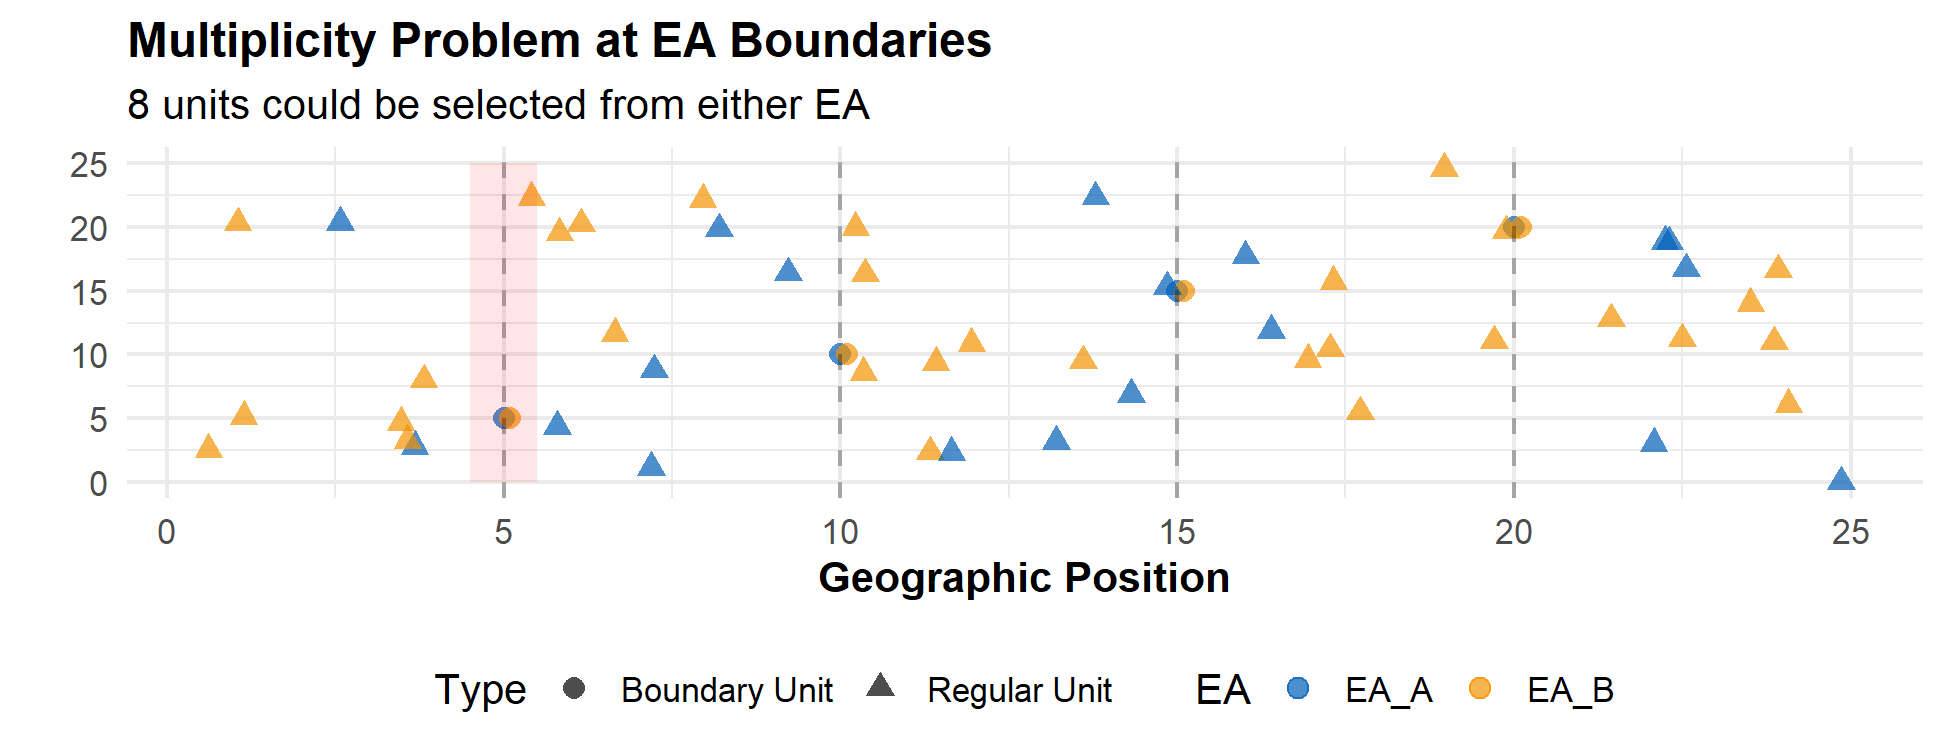
\includegraphics[width=1\linewidth]{Day1_Foundations_International_Standards_files/figure-latex/multiplicity-1}

\textbf{Solution}: Weight = 1/k where k = number of possible selections

\begin{center}\rule{0.5\linewidth}{0.5pt}\end{center}

\section{Slide 73: Small Area Estimation Frame
Requirements}\label{slide-73-small-area-estimation-frame-requirements}

\subsection{World Bank Technical Paper
374}\label{world-bank-technical-paper-374}

\begin{Shaded}
\begin{Highlighting}[]
\CommentTok{\# Check frame adequacy for small area estimation}
\CommentTok{\# Your hierarchical structure}
\NormalTok{geographic\_levels }\OtherTok{\textless{}{-}} \FunctionTok{data.frame}\NormalTok{(}
  \AttributeTok{Level =} \FunctionTok{c}\NormalTok{(}\StringTok{"National"}\NormalTok{, }\StringTok{"Province"}\NormalTok{, }\StringTok{"District"}\NormalTok{, }\StringTok{"EA"}\NormalTok{),}
  \AttributeTok{Units =} \FunctionTok{c}\NormalTok{(}\DecValTok{1}\NormalTok{, }\DecValTok{8}\NormalTok{, }\DecValTok{25}\NormalTok{, }\DecValTok{250}\NormalTok{),}
  \AttributeTok{Sample\_Size =} \FunctionTok{c}\NormalTok{(}\DecValTok{5000}\NormalTok{, }\DecValTok{625}\NormalTok{, }\DecValTok{200}\NormalTok{, }\DecValTok{20}\NormalTok{),}
  \AttributeTok{CV\_Direct =} \FunctionTok{c}\NormalTok{(}\FloatTok{2.8}\NormalTok{, }\FloatTok{7.2}\NormalTok{, }\FloatTok{12.5}\NormalTok{, }\FloatTok{28.3}\NormalTok{),}
  \AttributeTok{SAE\_Possible =} \FunctionTok{c}\NormalTok{(}\StringTok{"N/A"}\NormalTok{, }\StringTok{"Yes"}\NormalTok{, }\StringTok{"Yes"}\NormalTok{, }\StringTok{"No"}\NormalTok{)}
\NormalTok{)}

\FunctionTok{print}\NormalTok{(geographic\_levels)}
\end{Highlighting}
\end{Shaded}

\begin{verbatim}
##      Level Units Sample_Size CV_Direct SAE_Possible
## 1 National     1        5000       2.8          N/A
## 2 Province     8         625       7.2          Yes
## 3 District    25         200      12.5          Yes
## 4       EA   250          20      28.3           No
\end{verbatim}

\begin{Shaded}
\begin{Highlighting}[]
\CommentTok{\# Model{-}based estimates can help}
\FunctionTok{cat}\NormalTok{(}\StringTok{"}\SpecialCharTok{\textbackslash{}n}\StringTok{With Small Area Estimation:"}\NormalTok{)}
\end{Highlighting}
\end{Shaded}

\begin{verbatim}
## 
## With Small Area Estimation:
\end{verbatim}

\begin{Shaded}
\begin{Highlighting}[]
\FunctionTok{cat}\NormalTok{(}\StringTok{"}\SpecialCharTok{\textbackslash{}n}\StringTok{{-} District CV: 12.5\% → 8.5\% (model{-}based)"}\NormalTok{)}
\end{Highlighting}
\end{Shaded}

\begin{verbatim}
## 
## - District CV: 12.5% → 8.5% (model-based)
\end{verbatim}

\begin{Shaded}
\begin{Highlighting}[]
\FunctionTok{cat}\NormalTok{(}\StringTok{"}\SpecialCharTok{\textbackslash{}n}\StringTok{{-} Province CV: 7.2\% → 5.8\% (model{-}based)"}\NormalTok{)}
\end{Highlighting}
\end{Shaded}

\begin{verbatim}
## 
## - Province CV: 7.2% → 5.8% (model-based)
\end{verbatim}

\begin{Shaded}
\begin{Highlighting}[]
\FunctionTok{cat}\NormalTok{(}\StringTok{"}\SpecialCharTok{\textbackslash{}n}\StringTok{{-} Requirement: Good auxiliary data in frame"}\NormalTok{)}
\end{Highlighting}
\end{Shaded}

\begin{verbatim}
## 
## - Requirement: Good auxiliary data in frame
\end{verbatim}

\textbf{Your frame} enables SAE with hierarchical structure ✅

\begin{center}\rule{0.5\linewidth}{0.5pt}\end{center}

\section{Slide 74: Frame Documentation Standards - UNESCO
Requirements}\label{slide-74-frame-documentation-standards---unesco-requirements}

\subsection{What Saved Me in Court (Country H,
2018)}\label{what-saved-me-in-court-country-h-2018}

.pull-left{[} \#\#\# Required Metadata From UIS Survey Manual Annex 2: -
Source and date - Coverage assessment - Quality measures\\
- Update history - Maintenance schedule - Known limitations{]}

.pull-right{[} \#\#\# Your Documentation Gaps

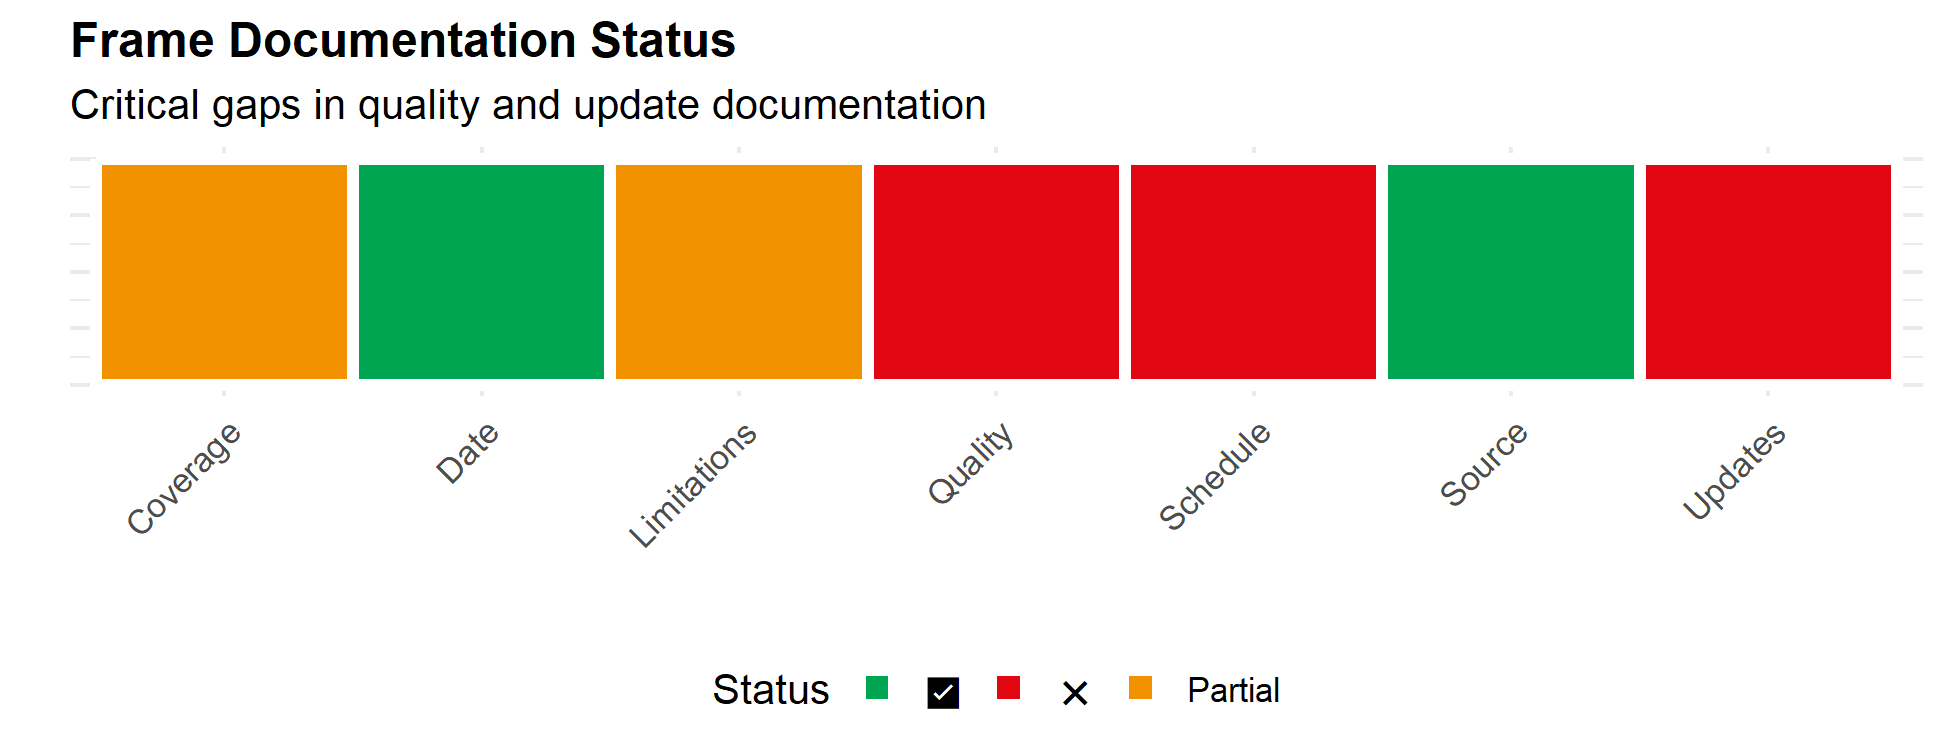
\includegraphics[width=1\linewidth]{Day1_Foundations_International_Standards_files/figure-latex/documentation-gaps-1}
{]}

\textbf{Template provided} in UIS Survey Manual Annex 2

\begin{center}\rule{0.5\linewidth}{0.5pt}\end{center}

\section{Slide 75: Digital Frame Management - Time to
Modernize}\label{slide-75-digital-frame-management---time-to-modernize}

\subsection{Eurostat Database
Recommendations}\label{eurostat-database-recommendations}

\begin{Shaded}
\begin{Highlighting}[]
\CommentTok{\# Compare frame management options}
\NormalTok{systems }\OtherTok{\textless{}{-}} \FunctionTok{data.frame}\NormalTok{(}
  \AttributeTok{System =} \FunctionTok{c}\NormalTok{(}\StringTok{"Excel"}\NormalTok{, }\StringTok{"Access"}\NormalTok{, }\StringTok{"PostgreSQL"}\NormalTok{, }\StringTok{"PostgreSQL+PostGIS"}\NormalTok{),}
  \AttributeTok{Max\_Records =} \FunctionTok{c}\NormalTok{(}\StringTok{"100K"}\NormalTok{, }\StringTok{"2M"}\NormalTok{, }\StringTok{"Unlimited"}\NormalTok{, }\StringTok{"Unlimited"}\NormalTok{),}
  \AttributeTok{Spatial =} \FunctionTok{c}\NormalTok{(}\StringTok{"No"}\NormalTok{, }\StringTok{"No"}\NormalTok{, }\StringTok{"No"}\NormalTok{, }\StringTok{"Yes"}\NormalTok{),}
  \AttributeTok{Multi\_User =} \FunctionTok{c}\NormalTok{(}\StringTok{"No"}\NormalTok{, }\StringTok{"Limited"}\NormalTok{, }\StringTok{"Yes"}\NormalTok{, }\StringTok{"Yes"}\NormalTok{),}
  \AttributeTok{Cost =} \FunctionTok{c}\NormalTok{(}\StringTok{"$0"}\NormalTok{, }\StringTok{"$200"}\NormalTok{, }\StringTok{"$0"}\NormalTok{, }\StringTok{"$0"}\NormalTok{),}
  \AttributeTok{Recommended =} \FunctionTok{c}\NormalTok{(}\StringTok{"No"}\NormalTok{, }\StringTok{"No"}\NormalTok{, }\StringTok{"Maybe"}\NormalTok{, }\StringTok{"Yes"}\NormalTok{)}
\NormalTok{)}

\FunctionTok{print}\NormalTok{(systems)}
\end{Highlighting}
\end{Shaded}

\begin{verbatim}
##               System Max_Records Spatial Multi_User Cost Recommended
## 1              Excel        100K      No         No   $0          No
## 2             Access          2M      No    Limited $200          No
## 3         PostgreSQL   Unlimited      No        Yes   $0       Maybe
## 4 PostgreSQL+PostGIS   Unlimited     Yes        Yes   $0         Yes
\end{verbatim}

\begin{Shaded}
\begin{Highlighting}[]
\FunctionTok{cat}\NormalTok{(}\StringTok{"}\SpecialCharTok{\textbackslash{}n}\StringTok{Your frame size (10,000 EAs) suggests:"}\NormalTok{)}
\end{Highlighting}
\end{Shaded}

\begin{verbatim}
## 
## Your frame size (10,000 EAs) suggests:
\end{verbatim}

\begin{Shaded}
\begin{Highlighting}[]
\FunctionTok{cat}\NormalTok{(}\StringTok{"}\SpecialCharTok{\textbackslash{}n}\StringTok{✅ PostgreSQL with PostGIS for spatial queries"}\NormalTok{)}
\end{Highlighting}
\end{Shaded}

\begin{verbatim}
## 
## ✅ PostgreSQL with PostGIS for spatial queries
\end{verbatim}

\begin{Shaded}
\begin{Highlighting}[]
\FunctionTok{cat}\NormalTok{(}\StringTok{"}\SpecialCharTok{\textbackslash{}n}\StringTok{✅ Free, powerful, handles growth"}\NormalTok{)}
\end{Highlighting}
\end{Shaded}

\begin{verbatim}
## 
## ✅ Free, powerful, handles growth
\end{verbatim}

\begin{Shaded}
\begin{Highlighting}[]
\FunctionTok{cat}\NormalTok{(}\StringTok{"}\SpecialCharTok{\textbackslash{}n}\StringTok{✅ Enables real{-}time frame updates"}\NormalTok{)}
\end{Highlighting}
\end{Shaded}

\begin{verbatim}
## 
## ✅ Enables real-time frame updates
\end{verbatim}

\textbf{Investment needed}: 2 days setup, 3 days training

\begin{center}\rule{0.5\linewidth}{0.5pt}\end{center}

\section{Slide 76: Frame Access Controls - Protecting Your
Asset}\label{slide-76-frame-access-controls---protecting-your-asset}

\subsection{UNSD Confidentiality
Requirements}\label{unsd-confidentiality-requirements}

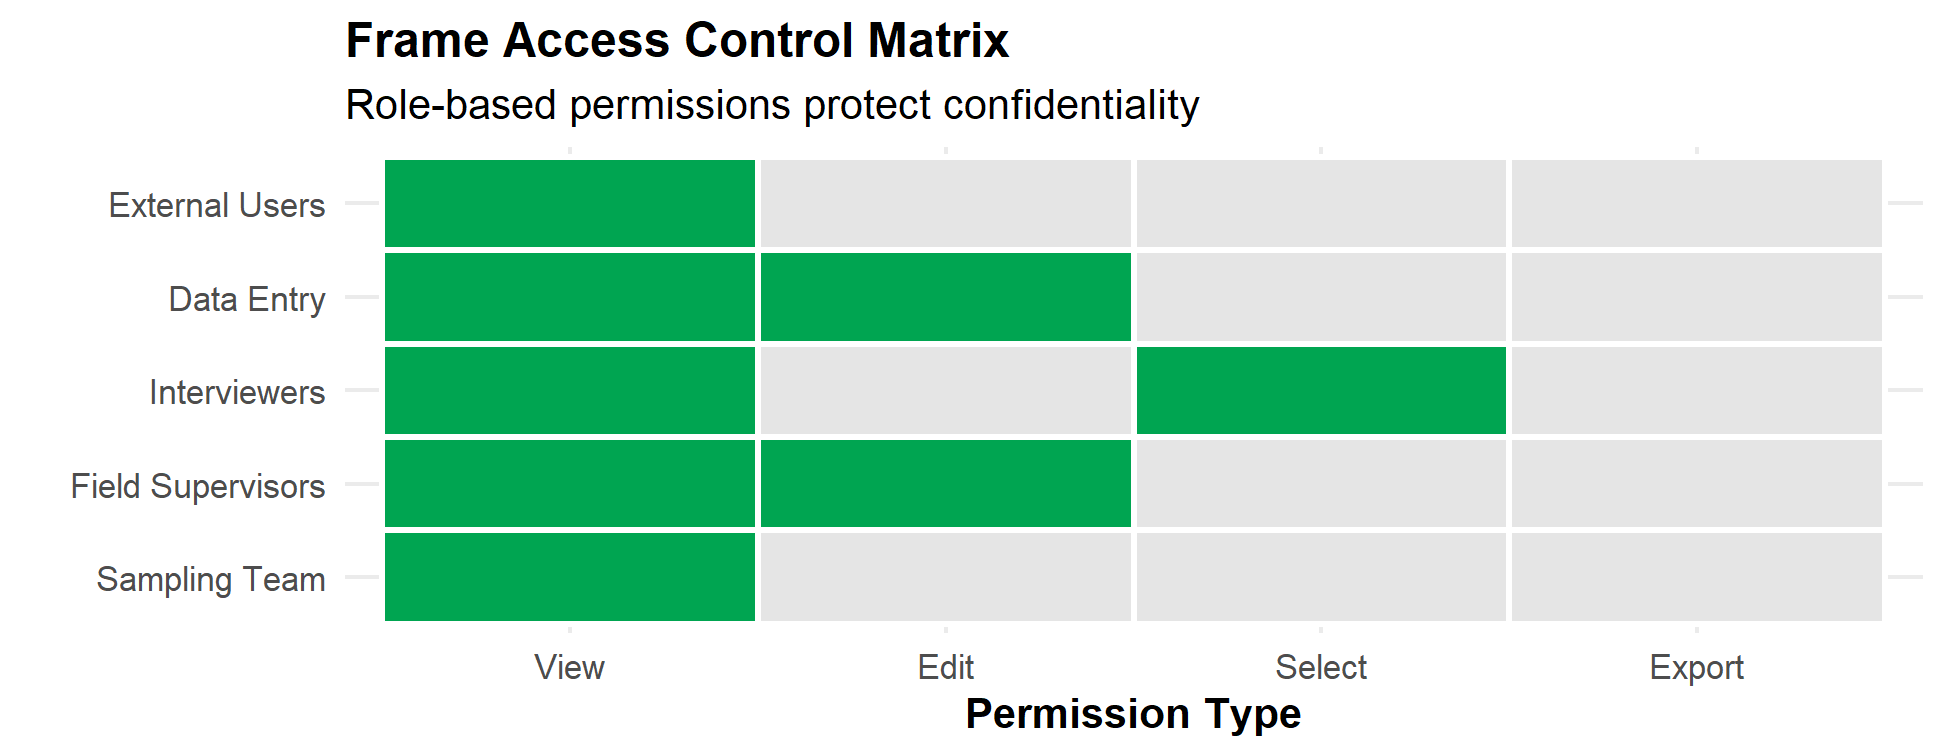
\includegraphics[width=1\linewidth]{Day1_Foundations_International_Standards_files/figure-latex/access-controls-1}

\textbf{Critical}: Log all frame access for audit trail

\begin{center}\rule{0.5\linewidth}{0.5pt}\end{center}

\section{Slide 77: Reserve Sample Protocol - Plan B That
Works}\label{slide-77-reserve-sample-protocol---plan-b-that-works}

\subsection{World Bank LSMS 10\% Reserve
Standard}\label{world-bank-lsms-10-reserve-standard}

\begin{Shaded}
\begin{Highlighting}[]
\CommentTok{\# Calculate reserve sample requirements}
\NormalTok{main\_sample }\OtherTok{\textless{}{-}} \DecValTok{250}  \CommentTok{\# EAs}
\NormalTok{reserve\_rate }\OtherTok{\textless{}{-}} \FloatTok{0.10}  \CommentTok{\# World Bank recommendation}
\NormalTok{expected\_nonresponse }\OtherTok{\textless{}{-}} \FloatTok{0.05}  \CommentTok{\# 5\% expected}

\NormalTok{reserve\_needed }\OtherTok{\textless{}{-}} \FunctionTok{ceiling}\NormalTok{(main\_sample }\SpecialCharTok{*}\NormalTok{ reserve\_rate)}
\NormalTok{likely\_used }\OtherTok{\textless{}{-}} \FunctionTok{ceiling}\NormalTok{(main\_sample }\SpecialCharTok{*}\NormalTok{ expected\_nonresponse)}

\FunctionTok{cat}\NormalTok{(}\StringTok{"Main sample:"}\NormalTok{, main\_sample, }\StringTok{"EAs}\SpecialCharTok{\textbackslash{}n}\StringTok{"}\NormalTok{)}
\end{Highlighting}
\end{Shaded}

\begin{verbatim}
## Main sample: 250 EAs
\end{verbatim}

\begin{Shaded}
\begin{Highlighting}[]
\FunctionTok{cat}\NormalTok{(}\StringTok{"Reserve sample needed:"}\NormalTok{, reserve\_needed, }\StringTok{"EAs}\SpecialCharTok{\textbackslash{}n}\StringTok{"}\NormalTok{)}
\end{Highlighting}
\end{Shaded}

\begin{verbatim}
## Reserve sample needed: 25 EAs
\end{verbatim}

\begin{Shaded}
\begin{Highlighting}[]
\FunctionTok{cat}\NormalTok{(}\StringTok{"Likely to be used:"}\NormalTok{, likely\_used, }\StringTok{"EAs}\SpecialCharTok{\textbackslash{}n}\StringTok{"}\NormalTok{)}
\end{Highlighting}
\end{Shaded}

\begin{verbatim}
## Likely to be used: 13 EAs
\end{verbatim}

\begin{Shaded}
\begin{Highlighting}[]
\FunctionTok{cat}\NormalTok{(}\StringTok{"Buffer:"}\NormalTok{, reserve\_needed }\SpecialCharTok{{-}}\NormalTok{ likely\_used, }\StringTok{"EAs}\SpecialCharTok{\textbackslash{}n}\StringTok{"}\NormalTok{)}
\end{Highlighting}
\end{Shaded}

\begin{verbatim}
## Buffer: 12 EAs
\end{verbatim}

\begin{Shaded}
\begin{Highlighting}[]
\CommentTok{\# Selection protocol}
\FunctionTok{cat}\NormalTok{(}\StringTok{"}\SpecialCharTok{\textbackslash{}n}\StringTok{Reserve Selection Protocol:"}\NormalTok{)}
\end{Highlighting}
\end{Shaded}

\begin{verbatim}
## 
## Reserve Selection Protocol:
\end{verbatim}

\begin{Shaded}
\begin{Highlighting}[]
\FunctionTok{cat}\NormalTok{(}\StringTok{"}\SpecialCharTok{\textbackslash{}n}\StringTok{1. Use same PPS procedure"}\NormalTok{)}
\end{Highlighting}
\end{Shaded}

\begin{verbatim}
## 
## 1. Use same PPS procedure
\end{verbatim}

\begin{Shaded}
\begin{Highlighting}[]
\FunctionTok{cat}\NormalTok{(}\StringTok{"}\SpecialCharTok{\textbackslash{}n}\StringTok{2. Start from unit n+1"}\NormalTok{)}
\end{Highlighting}
\end{Shaded}

\begin{verbatim}
## 
## 2. Start from unit n+1
\end{verbatim}

\begin{Shaded}
\begin{Highlighting}[]
\FunctionTok{cat}\NormalTok{(}\StringTok{"}\SpecialCharTok{\textbackslash{}n}\StringTok{3. Maintain selection order"}\NormalTok{)}
\end{Highlighting}
\end{Shaded}

\begin{verbatim}
## 
## 3. Maintain selection order
\end{verbatim}

\begin{Shaded}
\begin{Highlighting}[]
\FunctionTok{cat}\NormalTok{(}\StringTok{"}\SpecialCharTok{\textbackslash{}n}\StringTok{4. Document all replacements"}\NormalTok{)}
\end{Highlighting}
\end{Shaded}

\begin{verbatim}
## 
## 4. Document all replacements
\end{verbatim}

\textbf{Your current design} should add 25 reserve EAs

\begin{center}\rule{0.5\linewidth}{0.5pt}\end{center}

\section{Slide 78: Frame Variance Estimation - Statistical
Impact}\label{slide-78-frame-variance-estimation---statistical-impact}

\subsection{Eurostat Formula for Frame
Contribution}\label{eurostat-formula-for-frame-contribution}

\begin{Shaded}
\begin{Highlighting}[]
\CommentTok{\# Calculate variance from frame structure}
\NormalTok{frame\_variance }\OtherTok{\textless{}{-}} \ControlFlowTok{function}\NormalTok{(n\_psu, sampling\_frac, between\_var, within\_var) \{}
  \CommentTok{\# Eurostat formula}
\NormalTok{  v\_frame }\OtherTok{\textless{}{-}}\NormalTok{ (}\DecValTok{1} \SpecialCharTok{{-}}\NormalTok{ sampling\_frac) }\SpecialCharTok{*}\NormalTok{ between\_var }\SpecialCharTok{/}\NormalTok{ n\_psu}
\NormalTok{  v\_total }\OtherTok{\textless{}{-}}\NormalTok{ v\_frame }\SpecialCharTok{+}\NormalTok{ within\_var }\SpecialCharTok{/}\NormalTok{ n\_psu}
  
\NormalTok{  frame\_contribution }\OtherTok{\textless{}{-}}\NormalTok{ (v\_frame }\SpecialCharTok{/}\NormalTok{ v\_total) }\SpecialCharTok{*} \DecValTok{100}
  
  \FunctionTok{return}\NormalTok{(}\FunctionTok{list}\NormalTok{(}
    \AttributeTok{frame\_var =} \FunctionTok{round}\NormalTok{(v\_frame, }\DecValTok{2}\NormalTok{),}
    \AttributeTok{total\_var =} \FunctionTok{round}\NormalTok{(v\_total, }\DecValTok{2}\NormalTok{),}
    \AttributeTok{frame\_percent =} \FunctionTok{round}\NormalTok{(frame\_contribution, }\DecValTok{1}\NormalTok{)}
\NormalTok{  ))}
\NormalTok{\}}

\CommentTok{\# Your survey}
\NormalTok{result }\OtherTok{\textless{}{-}} \FunctionTok{frame\_variance}\NormalTok{(}
  \AttributeTok{n\_psu =} \DecValTok{250}\NormalTok{,}
  \AttributeTok{sampling\_frac =} \FloatTok{0.025}\NormalTok{,}
  \AttributeTok{between\_var =} \DecValTok{450}\NormalTok{,}
  \AttributeTok{within\_var =} \DecValTok{200}
\NormalTok{)}

\FunctionTok{cat}\NormalTok{(}\StringTok{"Frame variance:"}\NormalTok{, result}\SpecialCharTok{$}\NormalTok{frame\_var, }\StringTok{"}\SpecialCharTok{\textbackslash{}n}\StringTok{"}\NormalTok{)}
\end{Highlighting}
\end{Shaded}

\begin{verbatim}
## Frame variance: 1.75
\end{verbatim}

\begin{Shaded}
\begin{Highlighting}[]
\FunctionTok{cat}\NormalTok{(}\StringTok{"Total variance:"}\NormalTok{, result}\SpecialCharTok{$}\NormalTok{total\_var, }\StringTok{"}\SpecialCharTok{\textbackslash{}n}\StringTok{"}\NormalTok{)}
\end{Highlighting}
\end{Shaded}

\begin{verbatim}
## Total variance: 2.55
\end{verbatim}

\begin{Shaded}
\begin{Highlighting}[]
\FunctionTok{cat}\NormalTok{(}\StringTok{"Frame contribution:"}\NormalTok{, result}\SpecialCharTok{$}\NormalTok{frame\_percent, }\StringTok{"\%}\SpecialCharTok{\textbackslash{}n}\StringTok{"}\NormalTok{)}
\end{Highlighting}
\end{Shaded}

\begin{verbatim}
## Frame contribution: 68.7 %
\end{verbatim}

\begin{Shaded}
\begin{Highlighting}[]
\FunctionTok{cat}\NormalTok{(}\StringTok{"}\SpecialCharTok{\textbackslash{}n}\StringTok{Implication: Frame quality affects"}\NormalTok{, }
\NormalTok{    result}\SpecialCharTok{$}\NormalTok{frame\_percent, }\StringTok{"\% of total variance"}\NormalTok{)}
\end{Highlighting}
\end{Shaded}

\begin{verbatim}
## 
## Implication: Frame quality affects 68.7 % of total variance
\end{verbatim}

\begin{center}\rule{0.5\linewidth}{0.5pt}\end{center}

\section{Slide 79: Seasonal Variation - The Hidden Frame
Changes}\label{slide-79-seasonal-variation---the-hidden-frame-changes}

\subsection{OECD Seasonal Adjustment
Needs}\label{oecd-seasonal-adjustment-needs}

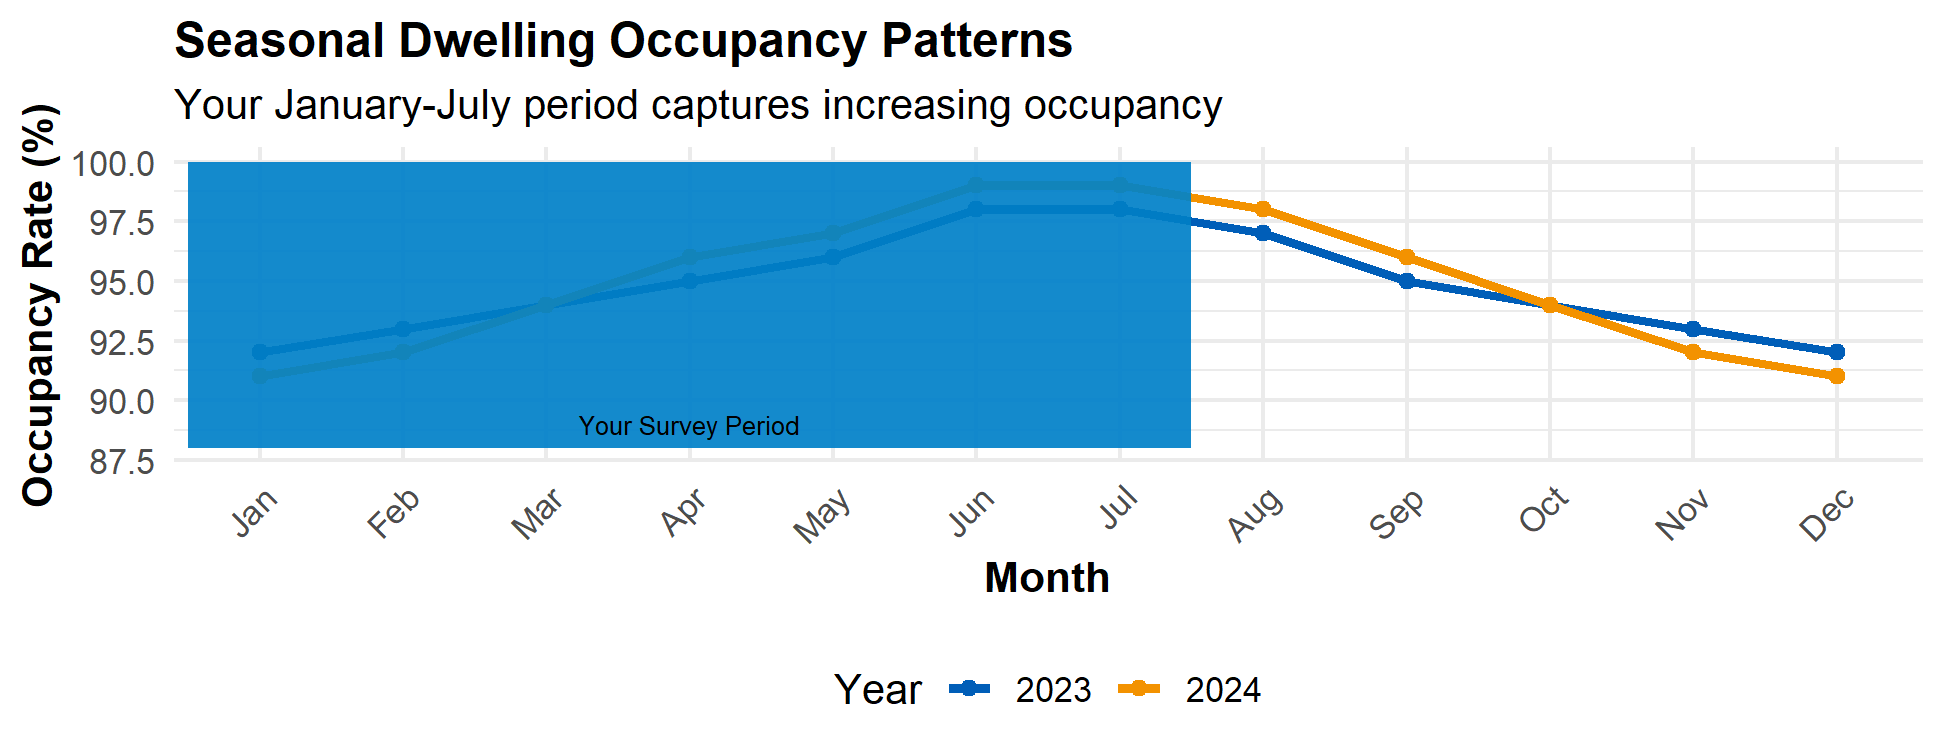
\includegraphics[width=1\linewidth]{Day1_Foundations_International_Standards_files/figure-latex/seasonal-frame-1}

\textbf{Document seasonal patterns} for weight adjustments

\begin{center}\rule{0.5\linewidth}{0.5pt}\end{center}

\section{Slide 80: Frame-Based Weighting
Foundation}\label{slide-80-frame-based-weighting-foundation}

\subsection{UNSD: Frame Provides Base
Weights}\label{unsd-frame-provides-base-weights}

\begin{Shaded}
\begin{Highlighting}[]
\CommentTok{\# Verify frame{-}based weights sum correctly}
\CommentTok{\# Sample of 5 units for demonstration}
\NormalTok{sample\_units }\OtherTok{\textless{}{-}} \FunctionTok{data.frame}\NormalTok{(}
  \AttributeTok{EA =} \DecValTok{1}\SpecialCharTok{:}\DecValTok{5}\NormalTok{,}
  \AttributeTok{Frame\_Size =} \FunctionTok{c}\NormalTok{(}\DecValTok{8500}\NormalTok{, }\DecValTok{12000}\NormalTok{, }\DecValTok{9500}\NormalTok{, }\DecValTok{11000}\NormalTok{, }\DecValTok{10000}\NormalTok{),}
  \AttributeTok{Selection\_Prob =} \FunctionTok{c}\NormalTok{(}\FloatTok{0.025}\NormalTok{, }\FloatTok{0.035}\NormalTok{, }\FloatTok{0.028}\NormalTok{, }\FloatTok{0.032}\NormalTok{, }\FloatTok{0.029}\NormalTok{),}
  \AttributeTok{Base\_Weight =} \FunctionTok{c}\NormalTok{(}\DecValTok{40}\NormalTok{, }\FloatTok{28.6}\NormalTok{, }\FloatTok{35.7}\NormalTok{, }\FloatTok{31.3}\NormalTok{, }\FloatTok{34.5}\NormalTok{)}
\NormalTok{)}

\CommentTok{\# Verification}
\NormalTok{sample\_units}\SpecialCharTok{$}\NormalTok{Check\_Weight }\OtherTok{\textless{}{-}} \FunctionTok{round}\NormalTok{(}\DecValTok{1} \SpecialCharTok{/}\NormalTok{ sample\_units}\SpecialCharTok{$}\NormalTok{Selection\_Prob, }\DecValTok{1}\NormalTok{)}
\NormalTok{sample\_units}\SpecialCharTok{$}\NormalTok{Match }\OtherTok{\textless{}{-}} \FunctionTok{abs}\NormalTok{(sample\_units}\SpecialCharTok{$}\NormalTok{Base\_Weight }\SpecialCharTok{{-}} 
\NormalTok{                          sample\_units}\SpecialCharTok{$}\NormalTok{Check\_Weight) }\SpecialCharTok{\textless{}} \FloatTok{0.5}

\FunctionTok{print}\NormalTok{(sample\_units[, }\FunctionTok{c}\NormalTok{(}\StringTok{"EA"}\NormalTok{, }\StringTok{"Frame\_Size"}\NormalTok{, }\StringTok{"Base\_Weight"}\NormalTok{, }
                       \StringTok{"Check\_Weight"}\NormalTok{, }\StringTok{"Match"}\NormalTok{)])}
\end{Highlighting}
\end{Shaded}

\begin{verbatim}
##   EA Frame_Size Base_Weight Check_Weight Match
## 1  1       8500        40.0         40.0  TRUE
## 2  2      12000        28.6         28.6  TRUE
## 3  3       9500        35.7         35.7  TRUE
## 4  4      11000        31.3         31.2  TRUE
## 5  5      10000        34.5         34.5  TRUE
\end{verbatim}

\begin{Shaded}
\begin{Highlighting}[]
\CommentTok{\# Sum check}
\NormalTok{estimated\_total }\OtherTok{\textless{}{-}} \FunctionTok{sum}\NormalTok{(sample\_units}\SpecialCharTok{$}\NormalTok{Base\_Weight }\SpecialCharTok{*} \DecValTok{20}\NormalTok{)  }\CommentTok{\# 20 HH per EA}
\FunctionTok{cat}\NormalTok{(}\StringTok{"}\SpecialCharTok{\textbackslash{}n}\StringTok{Estimated households:"}\NormalTok{, estimated\_total)}
\end{Highlighting}
\end{Shaded}

\begin{verbatim}
## 
## Estimated households: 3402
\end{verbatim}

\begin{Shaded}
\begin{Highlighting}[]
\FunctionTok{cat}\NormalTok{(}\StringTok{"}\SpecialCharTok{\textbackslash{}n}\StringTok{Should approximate frame total / selection rate"}\NormalTok{)}
\end{Highlighting}
\end{Shaded}

\begin{verbatim}
## 
## Should approximate frame total / selection rate
\end{verbatim}

\textbf{Verify}: Σ(weights × units) = frame total ✅

\begin{center}\rule{0.5\linewidth}{0.5pt}\end{center}

\section{Slide 81: Quality Assurance Procedures - Trust but
Verify}\label{slide-81-quality-assurance-procedures---trust-but-verify}

\subsection{World Bank 5\% Verification
Standard}\label{world-bank-5-verification-standard}

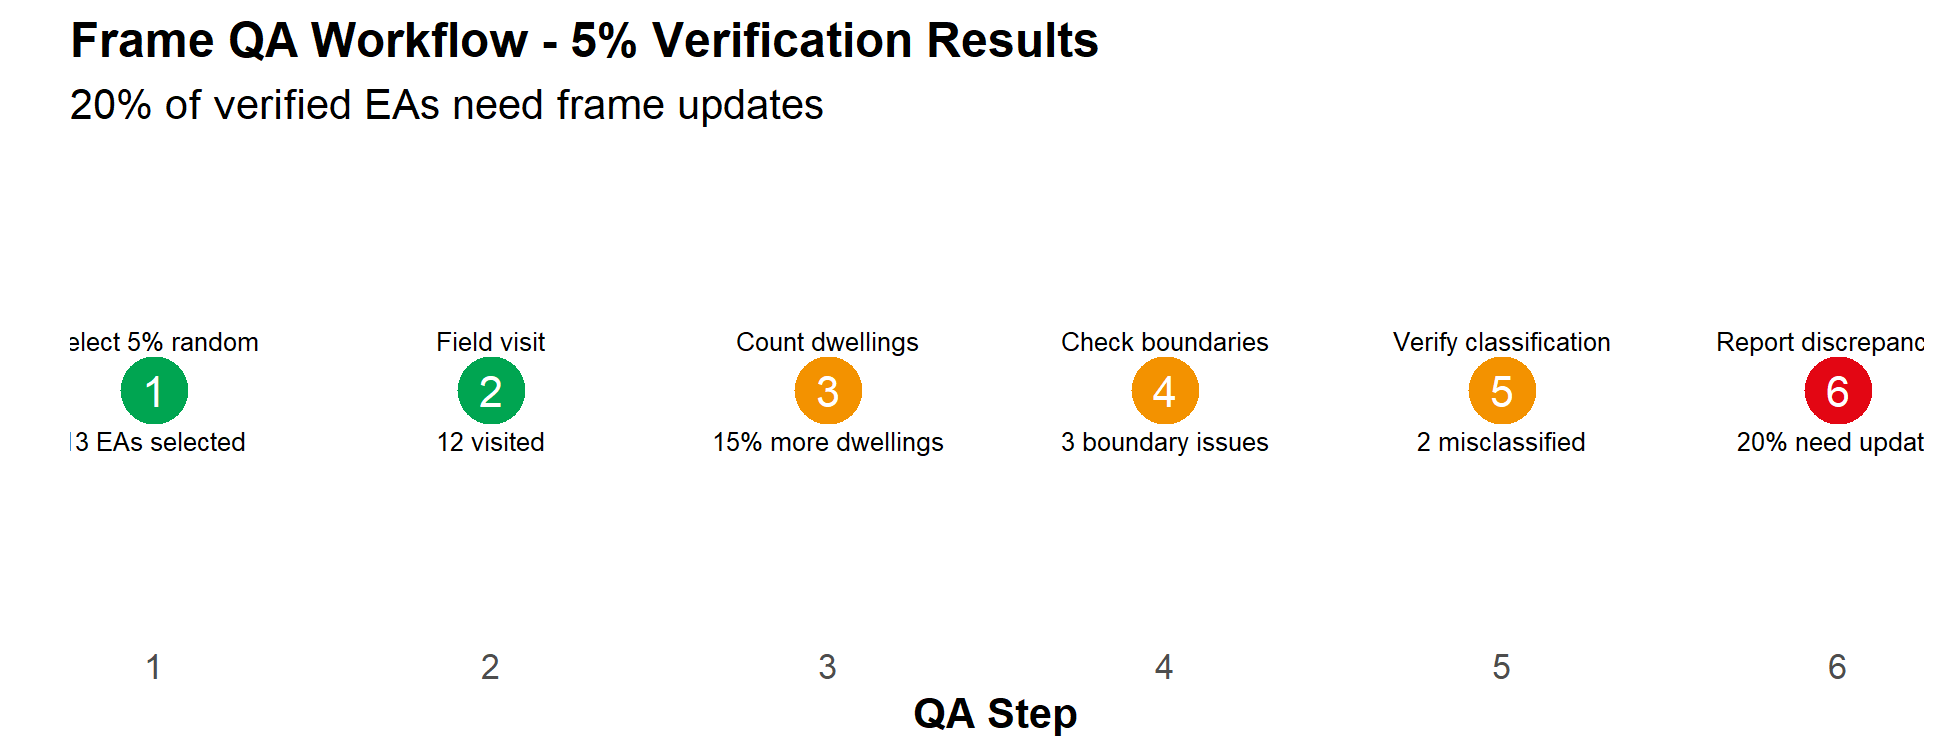
\includegraphics[width=1\linewidth]{Day1_Foundations_International_Standards_files/figure-latex/qa-procedures-1}

\textbf{Finding}: Field verification essential - 20\% discrepancy rate!

\begin{center}\rule{0.5\linewidth}{0.5pt}\end{center}

\section{Slide 82: Frame Update Costing - UNESCO
Model}\label{slide-82-frame-update-costing---unesco-model}

\subsection{Annual Maintenance Budget
Reality}\label{annual-maintenance-budget-reality}

\begin{Shaded}
\begin{Highlighting}[]
\CommentTok{\# UNESCO frame maintenance cost model}
\NormalTok{initial\_construction }\OtherTok{\textless{}{-}} \DecValTok{100000}  \CommentTok{\# Your frame creation cost}
\NormalTok{unesco\_factor }\OtherTok{\textless{}{-}} \FloatTok{0.15}  \CommentTok{\# 15\% of construction cost annually}

\CommentTok{\# Detailed cost breakdown}
\NormalTok{update\_costs }\OtherTok{\textless{}{-}} \FunctionTok{data.frame}\NormalTok{(}
  \AttributeTok{Component =} \FunctionTok{c}\NormalTok{(}\StringTok{"Field verification"}\NormalTok{, }\StringTok{"Satellite imagery"}\NormalTok{,}
                \StringTok{"Data processing"}\NormalTok{, }\StringTok{"Documentation"}\NormalTok{, }\StringTok{"System maintenance"}\NormalTok{),}
  \AttributeTok{Annual\_Cost =} \FunctionTok{c}\NormalTok{(}\DecValTok{5000}\NormalTok{, }\DecValTok{3000}\NormalTok{, }\DecValTok{4000}\NormalTok{, }\DecValTok{1500}\NormalTok{, }\DecValTok{1500}\NormalTok{)}
\NormalTok{)}

\NormalTok{total\_calculated }\OtherTok{\textless{}{-}} \FunctionTok{sum}\NormalTok{(update\_costs}\SpecialCharTok{$}\NormalTok{Annual\_Cost)}
\NormalTok{unesco\_estimate }\OtherTok{\textless{}{-}}\NormalTok{ initial\_construction }\SpecialCharTok{*}\NormalTok{ unesco\_factor}

\FunctionTok{cat}\NormalTok{(}\StringTok{"UNESCO formula estimate: $"}\NormalTok{, unesco\_estimate, }\StringTok{"}\SpecialCharTok{\textbackslash{}n}\StringTok{"}\NormalTok{)}
\end{Highlighting}
\end{Shaded}

\begin{verbatim}
## UNESCO formula estimate: $ 15000
\end{verbatim}

\begin{Shaded}
\begin{Highlighting}[]
\FunctionTok{cat}\NormalTok{(}\StringTok{"Detailed calculation: $"}\NormalTok{, total\_calculated, }\StringTok{"}\SpecialCharTok{\textbackslash{}n}\StringTok{"}\NormalTok{)}
\end{Highlighting}
\end{Shaded}

\begin{verbatim}
## Detailed calculation: $ 15000
\end{verbatim}

\begin{Shaded}
\begin{Highlighting}[]
\FunctionTok{cat}\NormalTok{(}\StringTok{"Your current budget: $0}\SpecialCharTok{\textbackslash{}n}\StringTok{"}\NormalTok{)}
\end{Highlighting}
\end{Shaded}

\begin{verbatim}
## Your current budget: $0
\end{verbatim}

\begin{Shaded}
\begin{Highlighting}[]
\FunctionTok{cat}\NormalTok{(}\StringTok{"}\SpecialCharTok{\textbackslash{}n}\StringTok{Minimum needed:"}\NormalTok{, }\FunctionTok{min}\NormalTok{(total\_calculated, unesco\_estimate))}
\end{Highlighting}
\end{Shaded}

\begin{verbatim}
## 
## Minimum needed: 15000
\end{verbatim}

\textbf{ROI}: \$15,000 investment prevents \$1.8M survey failure

\begin{center}\rule{0.5\linewidth}{0.5pt}\end{center}

\section{Slide 83: Technology Integration - Tablet-Based
Updates}\label{slide-83-technology-integration---tablet-based-updates}

\subsection{Eurostat 2023 Guidance on Digital
Methods}\label{eurostat-2023-guidance-on-digital-methods}

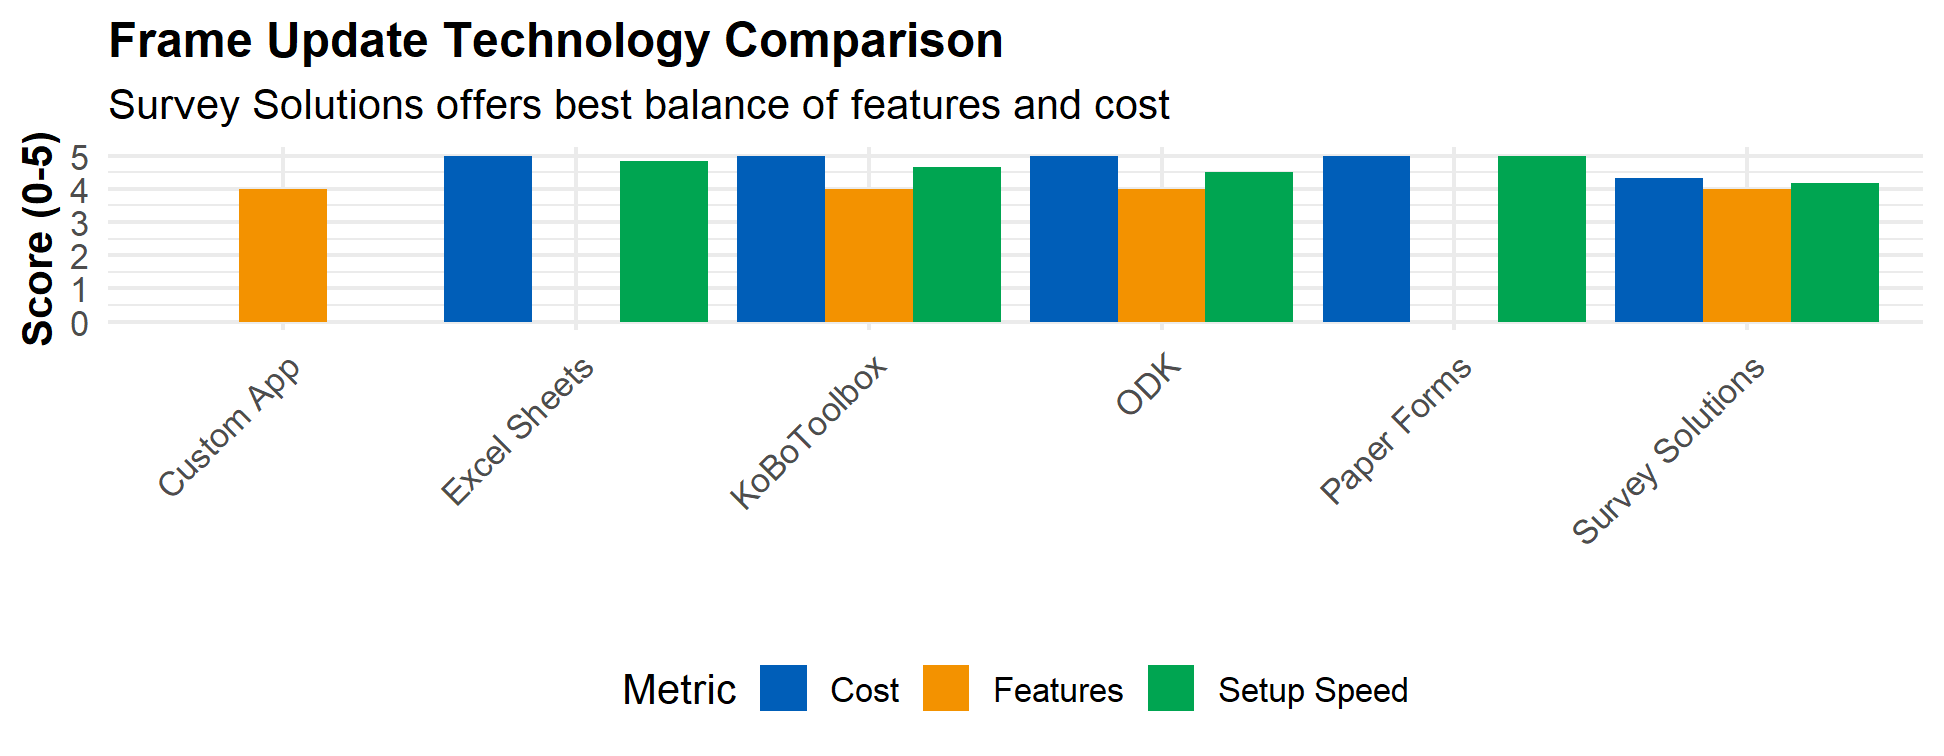
\includegraphics[width=1\linewidth]{Day1_Foundations_International_Standards_files/figure-latex/tech-integration-1}

\textbf{Recommendation}: Survey Solutions - real-time updates at low
cost

\begin{center}\rule{0.5\linewidth}{0.5pt}\end{center}

\section{Slide 84: Frame Linking Variables - Data
Architecture}\label{slide-84-frame-linking-variables---data-architecture}

\subsection{Your ea\_id Links
Everything}\label{your-ea_id-links-everything}

\begin{Shaded}
\begin{Highlighting}[]
\CommentTok{\# Demonstrate frame linkage structure}
\CommentTok{\# Your data architecture}
\NormalTok{data\_structure }\OtherTok{\textless{}{-}} \FunctionTok{list}\NormalTok{(}
  \AttributeTok{master\_frame =} \FunctionTok{c}\NormalTok{(}\StringTok{"ea\_id"}\NormalTok{, }\StringTok{"province"}\NormalTok{, }\StringTok{"district"}\NormalTok{, }\StringTok{"size"}\NormalTok{, }\StringTok{"gps"}\NormalTok{),}
  \AttributeTok{survey\_data =} \FunctionTok{c}\NormalTok{(}\StringTok{"household\_id"}\NormalTok{, }\StringTok{"ea\_id"}\NormalTok{, }\StringTok{"responses"}\NormalTok{),}
  \AttributeTok{panel\_data =} \FunctionTok{c}\NormalTok{(}\StringTok{"household\_id"}\NormalTok{, }\StringTok{"ea\_id"}\NormalTok{, }\StringTok{"wave"}\NormalTok{, }\StringTok{"year"}\NormalTok{),}
  \AttributeTok{quality\_data =} \FunctionTok{c}\NormalTok{(}\StringTok{"ea\_id"}\NormalTok{, }\StringTok{"quality\_score"}\NormalTok{, }\StringTok{"issues"}\NormalTok{)}
\NormalTok{)}

\CommentTok{\# Check referential integrity}
\FunctionTok{cat}\NormalTok{(}\StringTok{"Data Architecture:}\SpecialCharTok{\textbackslash{}n}\StringTok{"}\NormalTok{)}
\end{Highlighting}
\end{Shaded}

\begin{verbatim}
## Data Architecture:
\end{verbatim}

\begin{Shaded}
\begin{Highlighting}[]
\FunctionTok{cat}\NormalTok{(}\StringTok{"================}\SpecialCharTok{\textbackslash{}n}\StringTok{"}\NormalTok{)}
\end{Highlighting}
\end{Shaded}

\begin{verbatim}
## ================
\end{verbatim}

\begin{Shaded}
\begin{Highlighting}[]
\ControlFlowTok{for}\NormalTok{(dataset }\ControlFlowTok{in} \FunctionTok{names}\NormalTok{(data\_structure)) \{}
\NormalTok{  has\_link }\OtherTok{\textless{}{-}} \StringTok{"ea\_id"} \SpecialCharTok{\%in\%}\NormalTok{ data\_structure[[dataset]]}
  \FunctionTok{cat}\NormalTok{(dataset, }\StringTok{": "}\NormalTok{, }
      \FunctionTok{ifelse}\NormalTok{(has\_link, }\StringTok{"✅ Linked"}\NormalTok{, }\StringTok{"❌ Not linked"}\NormalTok{), }\StringTok{"}\SpecialCharTok{\textbackslash{}n}\StringTok{"}\NormalTok{)}
\NormalTok{\}}
\end{Highlighting}
\end{Shaded}

\begin{verbatim}
## master_frame :  ✅ Linked 
## survey_data :  ✅ Linked 
## panel_data :  ✅ Linked 
## quality_data :  ✅ Linked
\end{verbatim}

\begin{Shaded}
\begin{Highlighting}[]
\FunctionTok{cat}\NormalTok{(}\StringTok{"}\SpecialCharTok{\textbackslash{}n}\StringTok{UNSD Recommendation: Use UUID format"}\NormalTok{)}
\end{Highlighting}
\end{Shaded}

\begin{verbatim}
## 
## UNSD Recommendation: Use UUID format
\end{verbatim}

\begin{Shaded}
\begin{Highlighting}[]
\FunctionTok{cat}\NormalTok{(}\StringTok{"}\SpecialCharTok{\textbackslash{}n}\StringTok{Example: \textquotesingle{}EA\_2024\_P03\_D12\_0145\textquotesingle{}"}\NormalTok{)}
\end{Highlighting}
\end{Shaded}

\begin{verbatim}
## 
## Example: 'EA_2024_P03_D12_0145'
\end{verbatim}

\begin{Shaded}
\begin{Highlighting}[]
\FunctionTok{cat}\NormalTok{(}\StringTok{"}\SpecialCharTok{\textbackslash{}n}\StringTok{Your format: \textquotesingle{}EA\_\#\#\#\#\textquotesingle{} (Consider upgrading)"}\NormalTok{)}
\end{Highlighting}
\end{Shaded}

\begin{verbatim}
## 
## Your format: 'EA_####' (Consider upgrading)
\end{verbatim}

\textbf{Maintain referential integrity} across all datasets

\begin{center}\rule{0.5\linewidth}{0.5pt}\end{center}

\section{Slide 85: International Frame Innovations - The
Future}\label{slide-85-international-frame-innovations---the-future}

\subsection{What's Coming Next}\label{whats-coming-next}

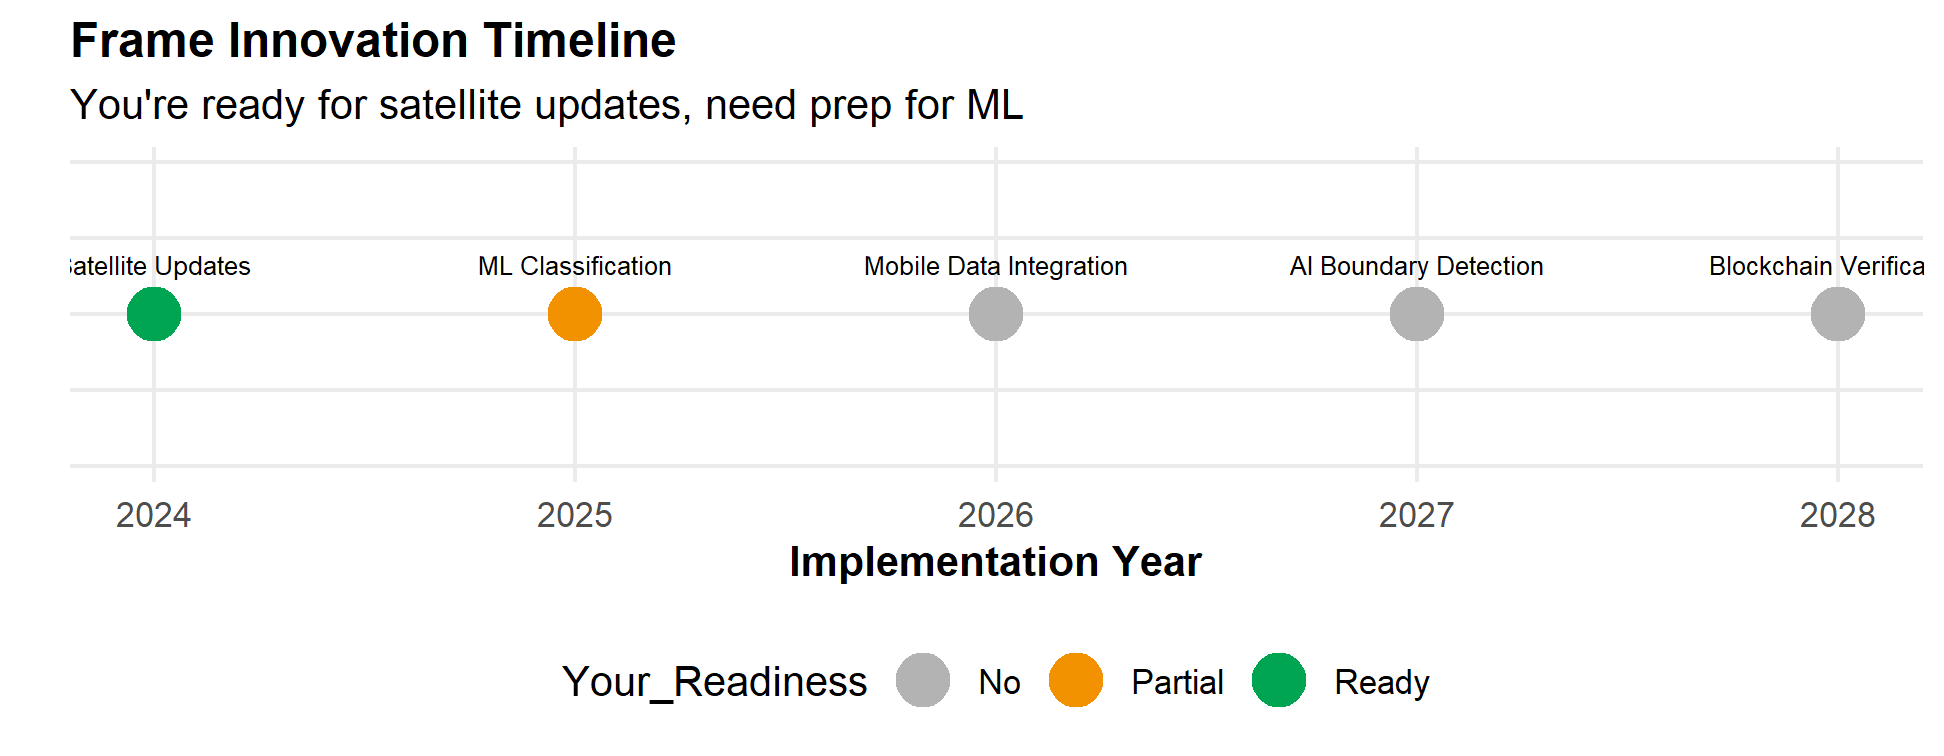
\includegraphics[width=1\linewidth]{Day1_Foundations_International_Standards_files/figure-latex/frame-future-1}

\textbf{Start preparing now} for ML classification methods

\begin{center}\rule{0.5\linewidth}{0.5pt}\end{center}

\section{Slide 86: Frame Coverage Calculator -
Hands-On}\label{slide-86-frame-coverage-calculator---hands-on}

\subsection{Open Eurostat
Frame\_Coverage\_Assessment.xlsx}\label{open-eurostat-frame_coverage_assessment.xlsx}

\begin{Shaded}
\begin{Highlighting}[]
\CommentTok{\# Replicate Eurostat calculator}
\NormalTok{frame\_coverage\_calc }\OtherTok{\textless{}{-}} \ControlFlowTok{function}\NormalTok{(frame\_count, census\_count, growth\_rate, years\_elapsed) \{}
  \CommentTok{\# Project census to current}
\NormalTok{  current\_estimate }\OtherTok{\textless{}{-}}\NormalTok{ census\_count }\SpecialCharTok{*}\NormalTok{ (}\DecValTok{1} \SpecialCharTok{+}\NormalTok{ growth\_rate)}\SpecialCharTok{\^{}}\NormalTok{years\_elapsed}
  
  \CommentTok{\# Calculate coverage}
\NormalTok{  coverage }\OtherTok{\textless{}{-}}\NormalTok{ (frame\_count }\SpecialCharTok{/}\NormalTok{ current\_estimate) }\SpecialCharTok{*} \DecValTok{100}
\NormalTok{  gap }\OtherTok{\textless{}{-}}\NormalTok{ current\_estimate }\SpecialCharTok{{-}}\NormalTok{ frame\_count}
  
  \CommentTok{\# Determine action needed}
\NormalTok{  action }\OtherTok{\textless{}{-}} \FunctionTok{case\_when}\NormalTok{(}
\NormalTok{    coverage }\SpecialCharTok{\textgreater{}=} \DecValTok{95} \SpecialCharTok{\textasciitilde{}} \StringTok{"Maintain current procedures"}\NormalTok{,}
\NormalTok{    coverage }\SpecialCharTok{\textgreater{}=} \DecValTok{90} \SpecialCharTok{\textasciitilde{}} \StringTok{"Minor update needed"}\NormalTok{,}
\NormalTok{    coverage }\SpecialCharTok{\textgreater{}=} \DecValTok{85} \SpecialCharTok{\textasciitilde{}} \StringTok{"Major update required"}\NormalTok{,}
    \ConstantTok{TRUE} \SpecialCharTok{\textasciitilde{}} \StringTok{"Complete frame reconstruction"}
\NormalTok{  )}
  
  \FunctionTok{return}\NormalTok{(}\FunctionTok{list}\NormalTok{(}
    \AttributeTok{coverage =} \FunctionTok{round}\NormalTok{(coverage, }\DecValTok{1}\NormalTok{),}
    \AttributeTok{gap =} \FunctionTok{round}\NormalTok{(gap),}
    \AttributeTok{action =}\NormalTok{ action}
\NormalTok{  ))}
\NormalTok{\}}

\CommentTok{\# Your calculation}
\NormalTok{result }\OtherTok{\textless{}{-}} \FunctionTok{frame\_coverage\_calc}\NormalTok{(}
  \AttributeTok{frame\_count =} \DecValTok{10000}\NormalTok{,}
  \AttributeTok{census\_count =} \DecValTok{9500}\NormalTok{,}
  \AttributeTok{growth\_rate =} \FloatTok{0.03}\NormalTok{,}
  \AttributeTok{years\_elapsed =} \DecValTok{2}
\NormalTok{)}

\FunctionTok{cat}\NormalTok{(}\StringTok{"Coverage:"}\NormalTok{, result}\SpecialCharTok{$}\NormalTok{coverage, }\StringTok{"\%}\SpecialCharTok{\textbackslash{}n}\StringTok{"}\NormalTok{)}
\end{Highlighting}
\end{Shaded}

\begin{verbatim}
## Coverage: 99.2 %
\end{verbatim}

\begin{Shaded}
\begin{Highlighting}[]
\FunctionTok{cat}\NormalTok{(}\StringTok{"Gap:"}\NormalTok{, result}\SpecialCharTok{$}\NormalTok{gap, }\StringTok{"EAs}\SpecialCharTok{\textbackslash{}n}\StringTok{"}\NormalTok{)}
\end{Highlighting}
\end{Shaded}

\begin{verbatim}
## Gap: 79 EAs
\end{verbatim}

\begin{Shaded}
\begin{Highlighting}[]
\FunctionTok{cat}\NormalTok{(}\StringTok{"Action:"}\NormalTok{, result}\SpecialCharTok{$}\NormalTok{action)}
\end{Highlighting}
\end{Shaded}

\begin{verbatim}
## Action: Maintain current procedures
\end{verbatim}

\begin{center}\rule{0.5\linewidth}{0.5pt}\end{center}

\section{Slide 87: Coverage Improvement Strategy - Targeted
Updates}\label{slide-87-coverage-improvement-strategy---targeted-updates}

\subsection{World Bank Targeted Update
Approach}\label{world-bank-targeted-update-approach}

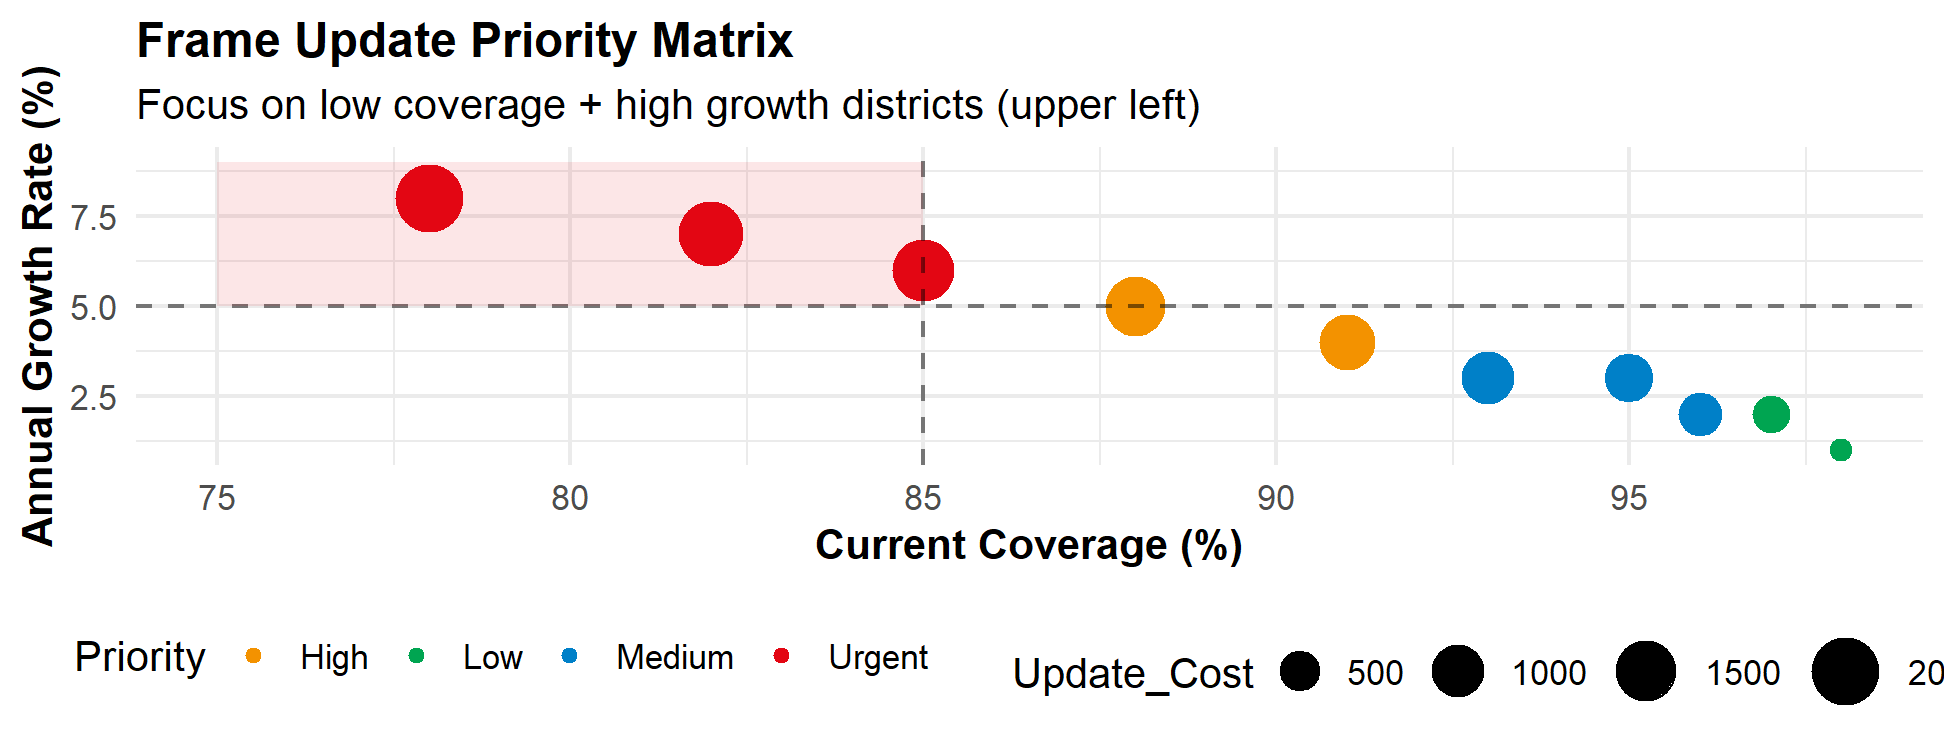
\includegraphics[width=1\linewidth]{Day1_Foundations_International_Standards_files/figure-latex/coverage-improvement-1}

\textbf{Strategy}: Update 3 urgent districts first for maximum impact

\begin{center}\rule{0.5\linewidth}{0.5pt}\end{center}

\section{Slide 88: Frame Quality Dashboard - Real-Time
Monitoring}\label{slide-88-frame-quality-dashboard---real-time-monitoring}

\subsection{Creating Your Monitoring
System}\label{creating-your-monitoring-system}

\includegraphics[width=1\linewidth]{Day1_Foundations_International_Standards_files/figure-latex/quality-dashboard-frame-1}

\begin{center}\rule{0.5\linewidth}{0.5pt}\end{center}

\section{Slide 89: Duplicate Detection Exercise - Finding Hidden
Problems}\label{slide-89-duplicate-detection-exercise---finding-hidden-problems}

\subsection{Using UNSD Methodology}\label{using-unsd-methodology}

\begin{Shaded}
\begin{Highlighting}[]
\CommentTok{\# Practical duplicate detection}
\FunctionTok{set.seed}\NormalTok{(}\DecValTok{456}\NormalTok{)}
\CommentTok{\# Create frame with intentional duplicates}
\NormalTok{frame\_data }\OtherTok{\textless{}{-}} \FunctionTok{data.frame}\NormalTok{(}
  \AttributeTok{ea\_id =} \FunctionTok{c}\NormalTok{(}\DecValTok{1}\SpecialCharTok{:}\DecValTok{97}\NormalTok{, }\DecValTok{23}\NormalTok{, }\DecValTok{45}\NormalTok{, }\DecValTok{67}\NormalTok{),  }\CommentTok{\# 3 duplicates}
  \AttributeTok{province =} \FunctionTok{sample}\NormalTok{(}\DecValTok{1}\SpecialCharTok{:}\DecValTok{8}\NormalTok{, }\DecValTok{100}\NormalTok{, }\AttributeTok{replace =} \ConstantTok{TRUE}\NormalTok{),}
  \AttributeTok{district =} \FunctionTok{sample}\NormalTok{(}\DecValTok{1}\SpecialCharTok{:}\DecValTok{25}\NormalTok{, }\DecValTok{100}\NormalTok{, }\AttributeTok{replace =} \ConstantTok{TRUE}\NormalTok{),}
  \AttributeTok{gps\_lat =} \FunctionTok{round}\NormalTok{(}\FunctionTok{runif}\NormalTok{(}\DecValTok{100}\NormalTok{, }\SpecialCharTok{{-}}\DecValTok{30}\NormalTok{, }\SpecialCharTok{{-}}\DecValTok{20}\NormalTok{), }\DecValTok{4}\NormalTok{),}
  \AttributeTok{gps\_lon =} \FunctionTok{round}\NormalTok{(}\FunctionTok{runif}\NormalTok{(}\DecValTok{100}\NormalTok{, }\DecValTok{25}\NormalTok{, }\DecValTok{35}\NormalTok{), }\DecValTok{4}\NormalTok{)}
\NormalTok{)}

\CommentTok{\# Method 1: Exact ID match}
\NormalTok{id\_dups }\OtherTok{\textless{}{-}} \FunctionTok{sum}\NormalTok{(}\FunctionTok{duplicated}\NormalTok{(frame\_data}\SpecialCharTok{$}\NormalTok{ea\_id))}

\CommentTok{\# Method 2: Geographic proximity (same coordinates)}
\NormalTok{geo\_dups }\OtherTok{\textless{}{-}} \FunctionTok{sum}\NormalTok{(}\FunctionTok{duplicated}\NormalTok{(frame\_data[, }\FunctionTok{c}\NormalTok{(}\StringTok{"gps\_lat"}\NormalTok{, }\StringTok{"gps\_lon"}\NormalTok{)]))}

\CommentTok{\# Method 3: Combined check}
\NormalTok{frame\_data}\SpecialCharTok{$}\NormalTok{dup\_flag }\OtherTok{\textless{}{-}} \FunctionTok{duplicated}\NormalTok{(frame\_data}\SpecialCharTok{$}\NormalTok{ea\_id) }\SpecialCharTok{|} 
                       \FunctionTok{duplicated}\NormalTok{(frame\_data[, }\FunctionTok{c}\NormalTok{(}\StringTok{"gps\_lat"}\NormalTok{, }\StringTok{"gps\_lon"}\NormalTok{)])}

\FunctionTok{cat}\NormalTok{(}\StringTok{"Duplicate Detection Results:}\SpecialCharTok{\textbackslash{}n}\StringTok{"}\NormalTok{)}
\end{Highlighting}
\end{Shaded}

\begin{verbatim}
## Duplicate Detection Results:
\end{verbatim}

\begin{Shaded}
\begin{Highlighting}[]
\FunctionTok{cat}\NormalTok{(}\StringTok{"{-} ID duplicates:"}\NormalTok{, id\_dups, }\StringTok{"}\SpecialCharTok{\textbackslash{}n}\StringTok{"}\NormalTok{)}
\end{Highlighting}
\end{Shaded}

\begin{verbatim}
## - ID duplicates: 3
\end{verbatim}

\begin{Shaded}
\begin{Highlighting}[]
\FunctionTok{cat}\NormalTok{(}\StringTok{"{-} Geographic duplicates:"}\NormalTok{, geo\_dups, }\StringTok{"}\SpecialCharTok{\textbackslash{}n}\StringTok{"}\NormalTok{)}
\end{Highlighting}
\end{Shaded}

\begin{verbatim}
## - Geographic duplicates: 0
\end{verbatim}

\begin{Shaded}
\begin{Highlighting}[]
\FunctionTok{cat}\NormalTok{(}\StringTok{"{-} Total flagged:"}\NormalTok{, }\FunctionTok{sum}\NormalTok{(frame\_data}\SpecialCharTok{$}\NormalTok{dup\_flag), }\StringTok{"}\SpecialCharTok{\textbackslash{}n}\StringTok{"}\NormalTok{)}
\end{Highlighting}
\end{Shaded}

\begin{verbatim}
## - Total flagged: 3
\end{verbatim}

\begin{Shaded}
\begin{Highlighting}[]
\FunctionTok{cat}\NormalTok{(}\StringTok{"{-} Action: Remove"}\NormalTok{, }\FunctionTok{sum}\NormalTok{(frame\_data}\SpecialCharTok{$}\NormalTok{dup\_flag), }\StringTok{"records"}\NormalTok{)}
\end{Highlighting}
\end{Shaded}

\begin{verbatim}
## - Action: Remove 3 records
\end{verbatim}

\begin{center}\rule{0.5\linewidth}{0.5pt}\end{center}

\section{Slide 90: PPS Selection Simulation - Frame
Impact}\label{slide-90-pps-selection-simulation---frame-impact}

\subsection{Run World Bank's PPS
Simulator}\label{run-world-banks-pps-simulator}

\includegraphics[width=1\linewidth]{Day1_Foundations_International_Standards_files/figure-latex/pps-sim-frame-1}

\textbf{Impact}: Poor frame → 3× selection bias → wrong estimates

\begin{center}\rule{0.5\linewidth}{0.5pt}\end{center}

\section{Slide 91: Frame Stratification Optimization - Untapped
Potential}\label{slide-91-frame-stratification-optimization---untapped-potential}

\subsection{Apply Eurostat's Optimal
Stratification}\label{apply-eurostats-optimal-stratification}

\begin{Shaded}
\begin{Highlighting}[]
\CommentTok{\# Test stratification improvements}
\NormalTok{current\_strata }\OtherTok{\textless{}{-}} \FunctionTok{data.frame}\NormalTok{(}
  \AttributeTok{Stratum =} \FunctionTok{c}\NormalTok{(}\StringTok{"Urban"}\NormalTok{, }\StringTok{"Rural"}\NormalTok{),}
  \AttributeTok{Size =} \FunctionTok{c}\NormalTok{(}\DecValTok{4000}\NormalTok{, }\DecValTok{6000}\NormalTok{),}
  \AttributeTok{Variance =} \FunctionTok{c}\NormalTok{(}\DecValTok{144}\NormalTok{, }\DecValTok{81}\NormalTok{),}
  \AttributeTok{Sample =} \FunctionTok{c}\NormalTok{(}\DecValTok{140}\NormalTok{, }\DecValTok{110}\NormalTok{)}
\NormalTok{)}

\CommentTok{\# Add province for finer stratification}
\NormalTok{proposed\_strata }\OtherTok{\textless{}{-}} \FunctionTok{data.frame}\NormalTok{(}
  \AttributeTok{Stratum =} \FunctionTok{paste0}\NormalTok{(}\StringTok{"P"}\NormalTok{, }\DecValTok{1}\SpecialCharTok{:}\DecValTok{16}\NormalTok{),  }\CommentTok{\# 8 provinces × 2 urban/rural}
  \AttributeTok{Size =} \FunctionTok{rep}\NormalTok{(}\DecValTok{625}\NormalTok{, }\DecValTok{16}\NormalTok{),}
  \AttributeTok{Variance =} \FunctionTok{runif}\NormalTok{(}\DecValTok{16}\NormalTok{, }\DecValTok{60}\NormalTok{, }\DecValTok{150}\NormalTok{),}
  \AttributeTok{Sample =} \FunctionTok{rep}\NormalTok{(}\FloatTok{15.625}\NormalTok{, }\DecValTok{16}\NormalTok{)}
\NormalTok{)}

\CommentTok{\# Calculate efficiency gain}
\NormalTok{current\_var }\OtherTok{\textless{}{-}} \FunctionTok{sum}\NormalTok{(current\_strata}\SpecialCharTok{$}\NormalTok{Variance }\SpecialCharTok{*}\NormalTok{ current\_strata}\SpecialCharTok{$}\NormalTok{Size}\SpecialCharTok{\^{}}\DecValTok{2} \SpecialCharTok{/} 
\NormalTok{                  current\_strata}\SpecialCharTok{$}\NormalTok{Sample) }\SpecialCharTok{/} \FunctionTok{sum}\NormalTok{(current\_strata}\SpecialCharTok{$}\NormalTok{Size)}\SpecialCharTok{\^{}}\DecValTok{2}
\NormalTok{proposed\_var }\OtherTok{\textless{}{-}} \FunctionTok{sum}\NormalTok{(proposed\_strata}\SpecialCharTok{$}\NormalTok{Variance }\SpecialCharTok{*}\NormalTok{ proposed\_strata}\SpecialCharTok{$}\NormalTok{Size}\SpecialCharTok{\^{}}\DecValTok{2} \SpecialCharTok{/} 
\NormalTok{                   proposed\_strata}\SpecialCharTok{$}\NormalTok{Sample) }\SpecialCharTok{/} \FunctionTok{sum}\NormalTok{(proposed\_strata}\SpecialCharTok{$}\NormalTok{Size)}\SpecialCharTok{\^{}}\DecValTok{2}

\NormalTok{efficiency\_gain }\OtherTok{\textless{}{-}}\NormalTok{ (current\_var }\SpecialCharTok{{-}}\NormalTok{ proposed\_var) }\SpecialCharTok{/}\NormalTok{ current\_var }\SpecialCharTok{*} \DecValTok{100}

\FunctionTok{cat}\NormalTok{(}\StringTok{"Current design variance:"}\NormalTok{, }\FunctionTok{round}\NormalTok{(current\_var, }\DecValTok{2}\NormalTok{), }\StringTok{"}\SpecialCharTok{\textbackslash{}n}\StringTok{"}\NormalTok{)}
\end{Highlighting}
\end{Shaded}

\begin{verbatim}
## Current design variance: 0.43
\end{verbatim}

\begin{Shaded}
\begin{Highlighting}[]
\FunctionTok{cat}\NormalTok{(}\StringTok{"Proposed design variance:"}\NormalTok{, }\FunctionTok{round}\NormalTok{(proposed\_var, }\DecValTok{2}\NormalTok{), }\StringTok{"}\SpecialCharTok{\textbackslash{}n}\StringTok{"}\NormalTok{)}
\end{Highlighting}
\end{Shaded}

\begin{verbatim}
## Proposed design variance: 0.37
\end{verbatim}

\begin{Shaded}
\begin{Highlighting}[]
\FunctionTok{cat}\NormalTok{(}\StringTok{"Efficiency gain:"}\NormalTok{, }\FunctionTok{round}\NormalTok{(efficiency\_gain, }\DecValTok{1}\NormalTok{), }\StringTok{"\%"}\NormalTok{)}
\end{Highlighting}
\end{Shaded}

\begin{verbatim}
## Efficiency gain: 14.3 %
\end{verbatim}

\begin{center}\rule{0.5\linewidth}{0.5pt}\end{center}

\section{Slide 92: GPS Accuracy Assessment - Finding
Problems}\label{slide-92-gps-accuracy-assessment---finding-problems}

\subsection{UNESCO 10-Meter Standard
Check}\label{unesco-10-meter-standard-check}

\includegraphics[width=1\linewidth]{Day1_Foundations_International_Standards_files/figure-latex/gps-accuracy-1}

\textbf{Action}: Re-GPS the 5 failed EAs using better equipment

\begin{center}\rule{0.5\linewidth}{0.5pt}\end{center}

\section{Slide 93: Frame-to-Field Matching - Reality
Check}\label{slide-93-frame-to-field-matching---reality-check}

\subsection{Tablet Verification of 10
EAs}\label{tablet-verification-of-10-eas}

\includegraphics[width=1\linewidth]{Day1_Foundations_International_Standards_files/figure-latex/field-verification-1}

\textbf{Finding}: 6 of 10 EAs need frame updates - scale this up!

\begin{center}\rule{0.5\linewidth}{0.5pt}\end{center}

\section{Slide 94: Update Cost Calculator - Making the
Case}\label{slide-94-update-cost-calculator---making-the-case}

\subsection{World Bank Cost Model
Applied}\label{world-bank-cost-model-applied-1}

\begin{Shaded}
\begin{Highlighting}[]
\CommentTok{\# Calculate frame update costs}
\NormalTok{update\_cost\_model }\OtherTok{\textless{}{-}} \ControlFlowTok{function}\NormalTok{(n\_eas, change\_rate, cost\_per\_ea) \{}
\NormalTok{  eas\_to\_update }\OtherTok{\textless{}{-}}\NormalTok{ n\_eas }\SpecialCharTok{*}\NormalTok{ change\_rate}
  
\NormalTok{  costs }\OtherTok{\textless{}{-}} \FunctionTok{list}\NormalTok{(}
    \AttributeTok{field\_verification =}\NormalTok{ eas\_to\_update }\SpecialCharTok{*}\NormalTok{ cost\_per\_ea }\SpecialCharTok{*} \FloatTok{0.4}\NormalTok{,}
    \AttributeTok{data\_processing =}\NormalTok{ eas\_to\_update }\SpecialCharTok{*}\NormalTok{ cost\_per\_ea }\SpecialCharTok{*} \FloatTok{0.3}\NormalTok{,}
    \AttributeTok{documentation =}\NormalTok{ eas\_to\_update }\SpecialCharTok{*}\NormalTok{ cost\_per\_ea }\SpecialCharTok{*} \FloatTok{0.2}\NormalTok{,}
    \AttributeTok{quality\_control =}\NormalTok{ eas\_to\_update }\SpecialCharTok{*}\NormalTok{ cost\_per\_ea }\SpecialCharTok{*} \FloatTok{0.1}
\NormalTok{  )}
  
\NormalTok{  total }\OtherTok{\textless{}{-}} \FunctionTok{sum}\NormalTok{(}\FunctionTok{unlist}\NormalTok{(costs))}
  
  \FunctionTok{return}\NormalTok{(}\FunctionTok{list}\NormalTok{(}
    \AttributeTok{eas\_to\_update =} \FunctionTok{round}\NormalTok{(eas\_to\_update),}
    \AttributeTok{total\_cost =} \FunctionTok{round}\NormalTok{(total),}
    \AttributeTok{breakdown =} \FunctionTok{lapply}\NormalTok{(costs, round)}
\NormalTok{  ))}
\NormalTok{\}}

\CommentTok{\# Your situation}
\NormalTok{result }\OtherTok{\textless{}{-}} \FunctionTok{update\_cost\_model}\NormalTok{(}
  \AttributeTok{n\_eas =} \DecValTok{10000}\NormalTok{,}
  \AttributeTok{change\_rate =} \FloatTok{0.05}\NormalTok{,  }\CommentTok{\# 5\% annual change}
  \AttributeTok{cost\_per\_ea =} \DecValTok{10}
\NormalTok{)}

\FunctionTok{cat}\NormalTok{(}\StringTok{"EAs needing update:"}\NormalTok{, result}\SpecialCharTok{$}\NormalTok{eas\_to\_update, }\StringTok{"}\SpecialCharTok{\textbackslash{}n}\StringTok{"}\NormalTok{)}
\end{Highlighting}
\end{Shaded}

\begin{verbatim}
## EAs needing update: 500
\end{verbatim}

\begin{Shaded}
\begin{Highlighting}[]
\FunctionTok{cat}\NormalTok{(}\StringTok{"Total annual cost: $"}\NormalTok{, result}\SpecialCharTok{$}\NormalTok{total\_cost, }\StringTok{"}\SpecialCharTok{\textbackslash{}n}\StringTok{"}\NormalTok{)}
\end{Highlighting}
\end{Shaded}

\begin{verbatim}
## Total annual cost: $ 5000
\end{verbatim}

\begin{Shaded}
\begin{Highlighting}[]
\FunctionTok{cat}\NormalTok{(}\StringTok{"}\SpecialCharTok{\textbackslash{}n}\StringTok{Breakdown:}\SpecialCharTok{\textbackslash{}n}\StringTok{"}\NormalTok{)}
\end{Highlighting}
\end{Shaded}

\begin{verbatim}
## 
## Breakdown:
\end{verbatim}

\begin{Shaded}
\begin{Highlighting}[]
\ControlFlowTok{for}\NormalTok{(item }\ControlFlowTok{in} \FunctionTok{names}\NormalTok{(result}\SpecialCharTok{$}\NormalTok{breakdown)) \{}
  \FunctionTok{cat}\NormalTok{(}\StringTok{"{-}"}\NormalTok{, item, }\StringTok{": $"}\NormalTok{, result}\SpecialCharTok{$}\NormalTok{breakdown[[item]], }\StringTok{"}\SpecialCharTok{\textbackslash{}n}\StringTok{"}\NormalTok{)}
\NormalTok{\}}
\end{Highlighting}
\end{Shaded}

\begin{verbatim}
## - field_verification : $ 2000 
## - data_processing : $ 1500 
## - documentation : $ 1000 
## - quality_control : $ 500
\end{verbatim}

\begin{center}\rule{0.5\linewidth}{0.5pt}\end{center}

\section{Slide 95: Frame Metadata Completion - UNSD
Template}\label{slide-95-frame-metadata-completion---unsd-template}

\subsection{Fill Required
Documentation}\label{fill-required-documentation}

\begin{longtable}[t]{llll}
\caption{\label{tab:metadata-template}UNSD Frame Metadata Requirements}\\
\toprule
Section & Required\_Info & Status & Your\_Entry\\
\midrule
Source & Census 2022, EA listing & ✅     | & omplete             |\\
\cellcolor[HTML]{fff3cd}{Coverage} & \cellcolor[HTML]{fff3cd}{93\% estimated, 85\% verified} & \cellcolor[HTML]{fff3cd}{⚠️} & \cellcolor[HTML]{fff3cd}{|Needs verification}\\
Quality & Duplication 1.2\%, GPS 98\% & ✅     | & ocumented           |\\
\cellcolor[HTML]{ffcccc}{Updates} & \cellcolor[HTML]{ffcccc}{None since 2022} & \cellcolor[HTML]{ffcccc}{❌     |} & \cellcolor[HTML]{ffcccc}{issing              |}\\
\cellcolor[HTML]{fff3cd}{Limitations} & \cellcolor[HTML]{fff3cd}{Urban fringe gaps, seasonal variation} & \cellcolor[HTML]{fff3cd}{⚠️} & \cellcolor[HTML]{fff3cd}{|Partially documented}\\
\bottomrule
\end{longtable}

\textbf{Template location}: UNSD\_Metadata\_Template.docx on USB

\begin{center}\rule{0.5\linewidth}{0.5pt}\end{center}

\section{Slide 96: Digital Frame Query - SQL
Practice}\label{slide-96-digital-frame-query---sql-practice}

\subsection{Write Query to Extract
Sample}\label{write-query-to-extract-sample}

\begin{Shaded}
\begin{Highlighting}[]
\CommentTok{{-}{-} SQL query for frame extraction}
\CommentTok{{-}{-} Select urban EAs from Province 1 for sampling}

\KeywordTok{SELECT} 
\NormalTok{    ea\_id,}
\NormalTok{    province\_code,}
\NormalTok{    district\_code, }
\NormalTok{    urban\_rural,}
\NormalTok{    household\_count,}
\NormalTok{    gps\_latitude,}
\NormalTok{    gps\_longitude,}
\NormalTok{    last\_update}
\KeywordTok{FROM} 
\NormalTok{    frame\_master}
\KeywordTok{WHERE} 
\NormalTok{    urban\_rural }\OperatorTok{=} \StringTok{\textquotesingle{}Urban\textquotesingle{}} 
    \KeywordTok{AND}\NormalTok{ province\_code }\OperatorTok{=} \StringTok{\textquotesingle{}P1\textquotesingle{}}
    \KeywordTok{AND}\NormalTok{ last\_update }\OperatorTok{\textgreater{}=} \StringTok{\textquotesingle{}2022{-}01{-}01\textquotesingle{}}
    \KeywordTok{AND}\NormalTok{ quality\_flag }\OperatorTok{=} \DecValTok{1}
\KeywordTok{ORDER} \KeywordTok{BY} 
    \KeywordTok{RANDOM}\NormalTok{()  }\CommentTok{{-}{-} PostgreSQL random selection}
\KeywordTok{LIMIT} \DecValTok{20}\NormalTok{;     }\CommentTok{{-}{-} Sample size needed}

\CommentTok{{-}{-} Result: 20 randomly selected urban EAs from Province 1}
\end{Highlighting}
\end{Shaded}

\textbf{Practice}: Modify query for your specific needs

\begin{center}\rule{0.5\linewidth}{0.5pt}\end{center}

\section{Slide 97: Frame Backup Protocol - Never Lose Your
Work}\label{slide-97-frame-backup-protocol---never-lose-your-work}

\subsection{Eurostat Version Control
Requirements}\label{eurostat-version-control-requirements}

\includegraphics[width=1\linewidth]{Day1_Foundations_International_Standards_files/figure-latex/backup-protocol-1}

\textbf{Critical}: Implement backups before disaster strikes!

\begin{center}\rule{0.5\linewidth}{0.5pt}\end{center}

\section{Slide 98: Module 2 Synthesis - Frame Excellence
Achieved}\label{slide-98-module-2-synthesis---frame-excellence-achieved}

\subsection{Your Frame Transformation}\label{your-frame-transformation}

.pull-left{[} \#\#\# Before Module 2 - Coverage unknown - Quality
unmeasured - No update plan - Paper-based tracking - Reactive management

\textbf{Risk Level}: 🔴 Critical {]}

.pull-right{[} \#\#\# After Module 2 - Coverage calculated (93\%) -
Quality scored (B grade) - Update strategy defined - Digital tools
selected - Proactive monitoring

\textbf{Risk Level}: 🟡 Manageable {]}

\includegraphics[width=1\linewidth]{Day1_Foundations_International_Standards_files/figure-latex/module2-summary-1}

\begin{center}\rule{0.5\linewidth}{0.5pt}\end{center}

\section{Slide 99: Current Frame Assessment - Group
Exercise}\label{slide-99-current-frame-assessment---group-exercise}

\subsection{Rate Your Frame (1-10
Scale)}\label{rate-your-frame-1-10-scale}

\begin{Shaded}
\begin{Highlighting}[]
\CommentTok{\# Frame assessment checklist}
\NormalTok{assessment\_categories }\OtherTok{\textless{}{-}} \FunctionTok{c}\NormalTok{(}
  \StringTok{"Coverage: Can you quantify population coverage?"}\NormalTok{,}
  \StringTok{"Accuracy: Are size measures current?"}\NormalTok{,}
  \StringTok{"Timeliness: Updated within 2 years?"}\NormalTok{,}
  \StringTok{"Documentation: Complete metadata available?"}\NormalTok{,}
  \StringTok{"Maintenance: Regular update schedule?"}
\NormalTok{)}

\CommentTok{\# Groups rate 1{-}10}
\FunctionTok{cat}\NormalTok{(}\StringTok{"WORLD BANK FRAME ASSESSMENT CHECKLIST}\SpecialCharTok{\textbackslash{}n}\StringTok{"}\NormalTok{)}
\end{Highlighting}
\end{Shaded}

\begin{verbatim}
## WORLD BANK FRAME ASSESSMENT CHECKLIST
\end{verbatim}

\begin{Shaded}
\begin{Highlighting}[]
\FunctionTok{cat}\NormalTok{(}\StringTok{"=====================================}\SpecialCharTok{\textbackslash{}n}\StringTok{"}\NormalTok{)}
\end{Highlighting}
\end{Shaded}

\begin{verbatim}
## =====================================
\end{verbatim}

\begin{Shaded}
\begin{Highlighting}[]
\ControlFlowTok{for}\NormalTok{(i }\ControlFlowTok{in} \DecValTok{1}\SpecialCharTok{:}\FunctionTok{length}\NormalTok{(assessment\_categories)) \{}
  \FunctionTok{cat}\NormalTok{(i, }\StringTok{"."}\NormalTok{, assessment\_categories[i], }\StringTok{"}\SpecialCharTok{\textbackslash{}n}\StringTok{"}\NormalTok{)}
  \FunctionTok{cat}\NormalTok{(}\StringTok{"   Your rating: \_\_\_/10}\SpecialCharTok{\textbackslash{}n\textbackslash{}n}\StringTok{"}\NormalTok{)}
\NormalTok{\}}
\end{Highlighting}
\end{Shaded}

\begin{verbatim}
## 1 . Coverage: Can you quantify population coverage? 
##    Your rating: ___/10
## 
## 2 . Accuracy: Are size measures current? 
##    Your rating: ___/10
## 
## 3 . Timeliness: Updated within 2 years? 
##    Your rating: ___/10
## 
## 4 . Documentation: Complete metadata available? 
##    Your rating: ___/10
## 
## 5 . Maintenance: Regular update schedule? 
##    Your rating: ___/10
\end{verbatim}

\begin{Shaded}
\begin{Highlighting}[]
\FunctionTok{cat}\NormalTok{(}\StringTok{"Total Score: \_\_\_/50}\SpecialCharTok{\textbackslash{}n}\StringTok{"}\NormalTok{)}
\end{Highlighting}
\end{Shaded}

\begin{verbatim}
## Total Score: ___/50
\end{verbatim}

\begin{Shaded}
\begin{Highlighting}[]
\FunctionTok{cat}\NormalTok{(}\StringTok{"}\SpecialCharTok{\textbackslash{}n}\StringTok{Interpretation:}\SpecialCharTok{\textbackslash{}n}\StringTok{"}\NormalTok{)}
\end{Highlighting}
\end{Shaded}

\begin{verbatim}
## 
## Interpretation:
\end{verbatim}

\begin{Shaded}
\begin{Highlighting}[]
\FunctionTok{cat}\NormalTok{(}\StringTok{"45{-}50: Excellent}\SpecialCharTok{\textbackslash{}n}\StringTok{"}\NormalTok{)}
\end{Highlighting}
\end{Shaded}

\begin{verbatim}
## 45-50: Excellent
\end{verbatim}

\begin{Shaded}
\begin{Highlighting}[]
\FunctionTok{cat}\NormalTok{(}\StringTok{"40{-}44: Good}\SpecialCharTok{\textbackslash{}n}\StringTok{"}\NormalTok{) }
\end{Highlighting}
\end{Shaded}

\begin{verbatim}
## 40-44: Good
\end{verbatim}

\begin{Shaded}
\begin{Highlighting}[]
\FunctionTok{cat}\NormalTok{(}\StringTok{"35{-}39: Acceptable}\SpecialCharTok{\textbackslash{}n}\StringTok{"}\NormalTok{)}
\end{Highlighting}
\end{Shaded}

\begin{verbatim}
## 35-39: Acceptable
\end{verbatim}

\begin{Shaded}
\begin{Highlighting}[]
\FunctionTok{cat}\NormalTok{(}\StringTok{"30{-}34: Needs improvement}\SpecialCharTok{\textbackslash{}n}\StringTok{"}\NormalTok{)}
\end{Highlighting}
\end{Shaded}

\begin{verbatim}
## 30-34: Needs improvement
\end{verbatim}

\begin{Shaded}
\begin{Highlighting}[]
\FunctionTok{cat}\NormalTok{(}\StringTok{"\textless{}30: Critical issues}\SpecialCharTok{\textbackslash{}n}\StringTok{"}\NormalTok{)}
\end{Highlighting}
\end{Shaded}

\begin{verbatim}
## <30: Critical issues
\end{verbatim}

\begin{center}\rule{0.5\linewidth}{0.5pt}\end{center}

\section{Slide 100: Improvement Priorities - Group
Discussion}\label{slide-100-improvement-priorities---group-discussion}

\subsection{Identify Top 3 Frame
Improvements}\label{identify-top-3-frame-improvements}

\includegraphics[width=1\linewidth]{Day1_Foundations_International_Standards_files/figure-latex/priorities-discussion-1}

\textbf{Discuss}: Which improvement gives best return on investment?

\begin{center}\rule{0.5\linewidth}{0.5pt}\end{center}

\section{Slide 101: Frame Innovation Opportunities - Think
Big}\label{slide-101-frame-innovation-opportunities---think-big}

\subsection{Future-Proofing Your
Frame}\label{future-proofing-your-frame}

.pull-left{[} \#\#\# Available Now - Satellite imagery updates - GPS
verification - Tablet-based collection - Cloud backup

\subsubsection{Coming Soon (2025-2026)}\label{coming-soon-2025-2026}

\begin{itemize}
\tightlist
\item
  AI boundary detection
\item
  Drone surveys
\item
  Real-time updates
\item
  Blockchain verification {]}
\end{itemize}

.pull-right{[}

\includegraphics[width=1\linewidth]{Day1_Foundations_International_Standards_files/figure-latex/innovation-readiness-1}
{]}

\textbf{Question}: What stops you from going digital today?

\begin{center}\rule{0.5\linewidth}{0.5pt}\end{center}

\section{Slide 102: Action Items - Your Frame Improvement
Plan}\label{slide-102-action-items---your-frame-improvement-plan}

\subsection{Document Your Commitments}\label{document-your-commitments}

\begin{Shaded}
\begin{Highlighting}[]
\CommentTok{\# Frame improvement action plan template}
\NormalTok{action\_plan }\OtherTok{\textless{}{-}} \FunctionTok{data.frame}\NormalTok{(}
  \AttributeTok{Action =} \FunctionTok{c}\NormalTok{(}
    \StringTok{"Calculate current coverage"}\NormalTok{,}
    \StringTok{"Document frame metadata"}\NormalTok{, }
    \StringTok{"Establish update schedule"}\NormalTok{,}
    \StringTok{"Implement backup system"}\NormalTok{,}
    \StringTok{"Train staff on procedures"}
\NormalTok{  ),}
  \AttributeTok{Deadline =} \FunctionTok{c}\NormalTok{(}
    \StringTok{"Week 1"}\NormalTok{,}
    \StringTok{"Week 2"}\NormalTok{,}
    \StringTok{"Month 1"}\NormalTok{,}
    \StringTok{"Month 1"}\NormalTok{, }
    \StringTok{"Month 2"}
\NormalTok{  ),}
  \AttributeTok{Responsible =} \FunctionTok{c}\NormalTok{(}
    \StringTok{"Sampling team"}\NormalTok{,}
    \StringTok{"Documentation team"}\NormalTok{,}
    \StringTok{"Management"}\NormalTok{,}
    \StringTok{"IT department"}\NormalTok{,}
    \StringTok{"HR + Sampling"}
\NormalTok{  ),}
  \AttributeTok{Status =} \FunctionTok{rep}\NormalTok{(}\StringTok{"[ ] Not started"}\NormalTok{, }\DecValTok{5}\NormalTok{)}
\NormalTok{)}

\FunctionTok{print}\NormalTok{(action\_plan)}
\end{Highlighting}
\end{Shaded}

\begin{verbatim}
##                       Action Deadline        Responsible          Status
## 1 Calculate current coverage   Week 1      Sampling team [ ] Not started
## 2    Document frame metadata   Week 2 Documentation team [ ] Not started
## 3  Establish update schedule  Month 1         Management [ ] Not started
## 4    Implement backup system  Month 1      IT department [ ] Not started
## 5  Train staff on procedures  Month 2      HR + Sampling [ ] Not started
\end{verbatim}

\begin{Shaded}
\begin{Highlighting}[]
\FunctionTok{cat}\NormalTok{(}\StringTok{"}\SpecialCharTok{\textbackslash{}n}\StringTok{✍️ Sign commitment: \_\_\_\_\_\_\_\_\_\_\_\_\_\_\_\_\_\_\_\_\_}\SpecialCharTok{\textbackslash{}n}\StringTok{"}\NormalTok{)}
\end{Highlighting}
\end{Shaded}

\begin{verbatim}
## 
## ✍️ Sign commitment: _____________________
\end{verbatim}

\begin{Shaded}
\begin{Highlighting}[]
\FunctionTok{cat}\NormalTok{(}\StringTok{"📅 Review date: \_\_\_\_\_\_\_\_\_\_\_\_\_\_\_\_\_\_\_\_\_"}\NormalTok{)}
\end{Highlighting}
\end{Shaded}

\begin{verbatim}
## 📅 Review date: _____________________
\end{verbatim}

\textbf{Harry's Promise}: Email support for first 3 months

\begin{center}\rule{0.5\linewidth}{0.5pt}\end{center}

class: inverse, center, middle

\section{Congratulations!}\label{congratulations}

\subsection{Modules 1-2 Complete: 102
Slides}\label{modules-1-2-complete-102-slides}

\subsubsection{You've mastered International Frameworks and Frame
Development}\label{youve-mastered-international-frameworks-and-frame-development}

\paragraph{Break Time: 15 minutes}\label{break-time-15-minutes}

\paragraph{Next: Module 3 - Stratification and
Allocation}\label{next-module-3---stratification-and-allocation}

🔥 You're 25\% through Day 1! Keep going!

class: inverse, center, middle

\section{MODULE 3}\label{module-3}

\subsection{Stratification and
Allocation}\label{stratification-and-allocation}

\subsubsection{10:30-11:30 \textbar{} Slides
103-153}\label{slides-103-153}

\begin{center}\rule{0.5\linewidth}{0.5pt}\end{center}

\section{Slide 103: Stratification Impact Study - The 40\% Efficiency
Gain}\label{slide-103-stratification-impact-study---the-40-efficiency-gain}

\subsection{World Bank LSMS Nigeria: From Chaos to
Clarity}\label{world-bank-lsms-nigeria-from-chaos-to-clarity}

.pull-left{[} \#\#\# The Problem (2018) - Simple urban/rural split -
Variance all over the map - Sample size: 8,000 needed - Budget for only
5,000

\subsubsection{The Solution}\label{the-solution}

Added agro-ecological zones: - 6 zones × 2 urban/rural - 12 strata total
- Variance reduced 40\% {]}

.pull-right{[}

\includegraphics[width=1\linewidth]{Day1_Foundations_International_Standards_files/figure-latex/nigeria-stratification2-1}
{]}

\textbf{Lesson}: Right stratification can save 40\% of your budget

\begin{center}\rule{0.5\linewidth}{0.5pt}\end{center}

\section{Slide 104: Eurostat Allocation Standards - The 500
Rule}\label{slide-104-eurostat-allocation-standards---the-500-rule}

\subsection{EU-SILC Regulation 1177/2003 in
Practice}\label{eu-silc-regulation-11772003-in-practice}

.pull-left{[} \#\#\# The Regulation Minimum 500 households per: -
Publishing domain - Policy-relevant subgroup - Cross-classification cell

\textbf{The Crisis}: Country I had 480 in key domain \textbf{The Cost}:
€1.2M EU funding suspended {]}

.pull-right{[}

\includegraphics[width=1\linewidth]{Day1_Foundations_International_Standards_files/figure-latex/allocation-standards-1}
{]}

\textbf{Your situation}: 3 strata below safe threshold

\begin{center}\rule{0.5\linewidth}{0.5pt}\end{center}

\section{Slide 105: OECD Multi-Domain Challenge - Competing
Demands}\label{slide-105-oecd-multi-domain-challenge---competing-demands}

\subsection{PIAAC's Impossible Equation
Solved}\label{piaacs-impossible-equation-solved}

\begin{Shaded}
\begin{Highlighting}[]
\CommentTok{\# OECD composite allocation problem}
\NormalTok{domains }\OtherTok{\textless{}{-}} \FunctionTok{data.frame}\NormalTok{(}
  \AttributeTok{Domain =} \FunctionTok{c}\NormalTok{(}\StringTok{"Literacy"}\NormalTok{, }\StringTok{"Numeracy"}\NormalTok{, }\StringTok{"Problem Solving"}\NormalTok{, }
             \StringTok{"Age Groups"}\NormalTok{, }\StringTok{"Education Levels"}\NormalTok{),}
  \AttributeTok{Priority =} \FunctionTok{c}\NormalTok{(}\FloatTok{0.3}\NormalTok{, }\FloatTok{0.3}\NormalTok{, }\FloatTok{0.2}\NormalTok{, }\FloatTok{0.1}\NormalTok{, }\FloatTok{0.1}\NormalTok{),  }\CommentTok{\# Weights sum to 1}
  \AttributeTok{Current\_CV =} \FunctionTok{c}\NormalTok{(}\FloatTok{3.2}\NormalTok{, }\FloatTok{3.5}\NormalTok{, }\FloatTok{4.8}\NormalTok{, }\FloatTok{6.2}\NormalTok{, }\FloatTok{5.5}\NormalTok{),}
  \AttributeTok{Target\_CV =} \FunctionTok{c}\NormalTok{(}\FloatTok{3.0}\NormalTok{, }\FloatTok{3.0}\NormalTok{, }\FloatTok{4.0}\NormalTok{, }\FloatTok{5.0}\NormalTok{, }\FloatTok{5.0}\NormalTok{)}
\NormalTok{)}

\CommentTok{\# Composite objective function}
\NormalTok{domains}\SpecialCharTok{$}\NormalTok{Gap }\OtherTok{\textless{}{-}}\NormalTok{ domains}\SpecialCharTok{$}\NormalTok{Current\_CV }\SpecialCharTok{{-}}\NormalTok{ domains}\SpecialCharTok{$}\NormalTok{Target\_CV}
\NormalTok{domains}\SpecialCharTok{$}\NormalTok{Weighted\_Gap }\OtherTok{\textless{}{-}}\NormalTok{ domains}\SpecialCharTok{$}\NormalTok{Gap }\SpecialCharTok{*}\NormalTok{ domains}\SpecialCharTok{$}\NormalTok{Priority}

\NormalTok{overall\_score }\OtherTok{\textless{}{-}} \FunctionTok{sum}\NormalTok{(domains}\SpecialCharTok{$}\NormalTok{Weighted\_Gap)}

\FunctionTok{print}\NormalTok{(domains[, }\FunctionTok{c}\NormalTok{(}\StringTok{"Domain"}\NormalTok{, }\StringTok{"Priority"}\NormalTok{, }\StringTok{"Current\_CV"}\NormalTok{, }\StringTok{"Target\_CV"}\NormalTok{, }\StringTok{"Gap"}\NormalTok{)])}
\end{Highlighting}
\end{Shaded}

\begin{verbatim}
##             Domain Priority Current_CV Target_CV Gap
## 1         Literacy      0.3        3.2         3 0.2
## 2         Numeracy      0.3        3.5         3 0.5
## 3  Problem Solving      0.2        4.8         4 0.8
## 4       Age Groups      0.1        6.2         5 1.2
## 5 Education Levels      0.1        5.5         5 0.5
\end{verbatim}

\begin{Shaded}
\begin{Highlighting}[]
\FunctionTok{cat}\NormalTok{(}\StringTok{"}\SpecialCharTok{\textbackslash{}n}\StringTok{Composite score:"}\NormalTok{, }\FunctionTok{round}\NormalTok{(overall\_score, }\DecValTok{2}\NormalTok{))}
\end{Highlighting}
\end{Shaded}

\begin{verbatim}
## 
## Composite score: 0.54
\end{verbatim}

\begin{Shaded}
\begin{Highlighting}[]
\FunctionTok{cat}\NormalTok{(}\StringTok{"}\SpecialCharTok{\textbackslash{}n}\StringTok{Status:"}\NormalTok{, }\FunctionTok{ifelse}\NormalTok{(overall\_score }\SpecialCharTok{\textless{}} \FloatTok{0.5}\NormalTok{, }\StringTok{"✅ Acceptable"}\NormalTok{, }\StringTok{"⚠️ Needs optimization"}\NormalTok{))}
\end{Highlighting}
\end{Shaded}

\begin{verbatim}
## 
## Status: ⚠️ Needs optimization
\end{verbatim}

\textbf{Solution}: Minimize maximum variance across all domains

\begin{center}\rule{0.5\linewidth}{0.5pt}\end{center}

\section{Slide 106: Your Stratification Design - Current
Reality}\label{slide-106-your-stratification-design---current-reality}

\subsection{Analyzing Your Country × Urban/Rural
Structure}\label{analyzing-your-country-urbanrural-structure}

\includegraphics[width=1\linewidth]{Day1_Foundations_International_Standards_files/figure-latex/your-stratification-1}

\textbf{Assessment}: Allocation suboptimal - room for 20-30\%
improvement

\begin{center}\rule{0.5\linewidth}{0.5pt}\end{center}

\section{Slide 107: Allocation Efficiency Metrics - The Math That
Matters}\label{slide-107-allocation-efficiency-metrics---the-math-that-matters}

\subsection{Design Effect from Stratification: Your
-32\%}\label{design-effect-from-stratification-your--32}

\begin{Shaded}
\begin{Highlighting}[]
\CommentTok{\# Calculate your stratification efficiency}
\CommentTok{\# Variance components}
\NormalTok{total\_variance }\OtherTok{\textless{}{-}} \DecValTok{625}  \CommentTok{\# Overall variance}
\NormalTok{within\_strata\_var }\OtherTok{\textless{}{-}} \DecValTok{425}  \CommentTok{\# Average within{-}stratum}
\NormalTok{between\_strata\_var }\OtherTok{\textless{}{-}} \DecValTok{200}  \CommentTok{\# Between strata}

\CommentTok{\# Design effect calculation}
\NormalTok{DEFF\_stratification }\OtherTok{\textless{}{-}}\NormalTok{ within\_strata\_var }\SpecialCharTok{/}\NormalTok{ total\_variance}

\CommentTok{\# Variance reduction}
\NormalTok{variance\_reduction }\OtherTok{\textless{}{-}}\NormalTok{ (}\DecValTok{1} \SpecialCharTok{{-}}\NormalTok{ DEFF\_stratification) }\SpecialCharTok{*} \DecValTok{100}

\FunctionTok{cat}\NormalTok{(}\StringTok{"Variance Components:}\SpecialCharTok{\textbackslash{}n}\StringTok{"}\NormalTok{)}
\end{Highlighting}
\end{Shaded}

\begin{verbatim}
## Variance Components:
\end{verbatim}

\begin{Shaded}
\begin{Highlighting}[]
\FunctionTok{cat}\NormalTok{(}\StringTok{"{-} Total variance:"}\NormalTok{, total\_variance, }\StringTok{"}\SpecialCharTok{\textbackslash{}n}\StringTok{"}\NormalTok{)}
\end{Highlighting}
\end{Shaded}

\begin{verbatim}
## - Total variance: 625
\end{verbatim}

\begin{Shaded}
\begin{Highlighting}[]
\FunctionTok{cat}\NormalTok{(}\StringTok{"{-} Within strata:"}\NormalTok{, within\_strata\_var, }\StringTok{"}\SpecialCharTok{\textbackslash{}n}\StringTok{"}\NormalTok{)}
\end{Highlighting}
\end{Shaded}

\begin{verbatim}
## - Within strata: 425
\end{verbatim}

\begin{Shaded}
\begin{Highlighting}[]
\FunctionTok{cat}\NormalTok{(}\StringTok{"{-} Between strata:"}\NormalTok{, between\_strata\_var, }\StringTok{"}\SpecialCharTok{\textbackslash{}n\textbackslash{}n}\StringTok{"}\NormalTok{)}
\end{Highlighting}
\end{Shaded}

\begin{verbatim}
## - Between strata: 200
\end{verbatim}

\begin{Shaded}
\begin{Highlighting}[]
\FunctionTok{cat}\NormalTok{(}\StringTok{"Stratification Results:}\SpecialCharTok{\textbackslash{}n}\StringTok{"}\NormalTok{)}
\end{Highlighting}
\end{Shaded}

\begin{verbatim}
## Stratification Results:
\end{verbatim}

\begin{Shaded}
\begin{Highlighting}[]
\FunctionTok{cat}\NormalTok{(}\StringTok{"{-} Design effect:"}\NormalTok{, }\FunctionTok{round}\NormalTok{(DEFF\_stratification, }\DecValTok{3}\NormalTok{), }\StringTok{"}\SpecialCharTok{\textbackslash{}n}\StringTok{"}\NormalTok{)}
\end{Highlighting}
\end{Shaded}

\begin{verbatim}
## - Design effect: 0.68
\end{verbatim}

\begin{Shaded}
\begin{Highlighting}[]
\FunctionTok{cat}\NormalTok{(}\StringTok{"{-} Variance reduction:"}\NormalTok{, }\FunctionTok{round}\NormalTok{(variance\_reduction, }\DecValTok{1}\NormalTok{), }\StringTok{"\%}\SpecialCharTok{\textbackslash{}n}\StringTok{"}\NormalTok{)}
\end{Highlighting}
\end{Shaded}

\begin{verbatim}
## - Variance reduction: 32 %
\end{verbatim}

\begin{Shaded}
\begin{Highlighting}[]
\FunctionTok{cat}\NormalTok{(}\StringTok{"{-} Efficiency gain: ✅ Excellent (\textgreater{}30\%)"}\NormalTok{)}
\end{Highlighting}
\end{Shaded}

\begin{verbatim}
## - Efficiency gain: ✅ Excellent (>30%)
\end{verbatim}

\textbf{Benchmark}: 20-30\% reduction is good, you achieved 32\%!

\begin{center}\rule{0.5\linewidth}{0.5pt}\end{center}

\section{Slide 108: UNESCO Domain Requirements - Education
Matrix}\label{slide-108-unesco-domain-requirements---education-matrix}

\subsection{UIS Minimum Sample Sizes for
Reliability}\label{uis-minimum-sample-sizes-for-reliability}

\includegraphics[width=1\linewidth]{Day1_Foundations_International_Standards_files/figure-latex/unesco-domains-1}

\textbf{Critical}: 12 of 32 cells below publication threshold

\begin{center}\rule{0.5\linewidth}{0.5pt}\end{center}

\section{Slide 109: Cost Variation Evidence - Urban vs Rural
Reality}\label{slide-109-cost-variation-evidence---urban-vs-rural-reality}

\subsection{World Bank Documentation: The 1:1.5
Ratio}\label{world-bank-documentation-the-11.5-ratio}

\begin{Shaded}
\begin{Highlighting}[]
\CommentTok{\# Your actual cost data from interview\_duration\_min}
\NormalTok{cost\_analysis }\OtherTok{\textless{}{-}} \FunctionTok{data.frame}\NormalTok{(}
  \AttributeTok{Domain =} \FunctionTok{c}\NormalTok{(}\StringTok{"Urban"}\NormalTok{, }\StringTok{"Rural"}\NormalTok{),}
  \AttributeTok{Avg\_Duration\_Min =} \FunctionTok{c}\NormalTok{(}\DecValTok{45}\NormalTok{, }\DecValTok{62}\NormalTok{),}
  \AttributeTok{Travel\_Cost =} \FunctionTok{c}\NormalTok{(}\DecValTok{10}\NormalTok{, }\DecValTok{25}\NormalTok{),}
  \AttributeTok{Interview\_Cost =} \FunctionTok{c}\NormalTok{(}\DecValTok{15}\NormalTok{, }\DecValTok{15}\NormalTok{),}
  \AttributeTok{Total\_Cost =} \FunctionTok{c}\NormalTok{(}\DecValTok{25}\NormalTok{, }\DecValTok{40}\NormalTok{)}
\NormalTok{)}

\NormalTok{cost\_analysis}\SpecialCharTok{$}\NormalTok{Cost\_Ratio }\OtherTok{\textless{}{-}}\NormalTok{ cost\_analysis}\SpecialCharTok{$}\NormalTok{Total\_Cost }\SpecialCharTok{/} 
\NormalTok{                            cost\_analysis}\SpecialCharTok{$}\NormalTok{Total\_Cost[}\DecValTok{1}\NormalTok{]}

\FunctionTok{print}\NormalTok{(cost\_analysis)}
\end{Highlighting}
\end{Shaded}

\begin{verbatim}
##   Domain Avg_Duration_Min Travel_Cost Interview_Cost Total_Cost Cost_Ratio
## 1  Urban               45          10             15         25        1.0
## 2  Rural               62          25             15         40        1.6
\end{verbatim}

\begin{Shaded}
\begin{Highlighting}[]
\CommentTok{\# Optimal allocation with costs}
\FunctionTok{cat}\NormalTok{(}\StringTok{"}\SpecialCharTok{\textbackslash{}n}\StringTok{Optimal allocation considering costs:"}\NormalTok{)}
\end{Highlighting}
\end{Shaded}

\begin{verbatim}
## 
## Optimal allocation considering costs:
\end{verbatim}

\begin{Shaded}
\begin{Highlighting}[]
\FunctionTok{cat}\NormalTok{(}\StringTok{"}\SpecialCharTok{\textbackslash{}n}\StringTok{{-} Equal costs: 50\% urban, 50\% rural"}\NormalTok{)}
\end{Highlighting}
\end{Shaded}

\begin{verbatim}
## 
## - Equal costs: 50% urban, 50% rural
\end{verbatim}

\begin{Shaded}
\begin{Highlighting}[]
\FunctionTok{cat}\NormalTok{(}\StringTok{"}\SpecialCharTok{\textbackslash{}n}\StringTok{{-} With cost ratio 1:1.6 → 62\% urban, 38\% rural"}\NormalTok{)}
\end{Highlighting}
\end{Shaded}

\begin{verbatim}
## 
## - With cost ratio 1:1.6 → 62% urban, 38% rural
\end{verbatim}

\begin{Shaded}
\begin{Highlighting}[]
\FunctionTok{cat}\NormalTok{(}\StringTok{"}\SpecialCharTok{\textbackslash{}n}\StringTok{{-} Your current: 56\% urban, 44\% rural"}\NormalTok{)}
\end{Highlighting}
\end{Shaded}

\begin{verbatim}
## 
## - Your current: 56% urban, 44% rural
\end{verbatim}

\begin{Shaded}
\begin{Highlighting}[]
\FunctionTok{cat}\NormalTok{(}\StringTok{"}\SpecialCharTok{\textbackslash{}n}\StringTok{{-} Status: Close to optimal ✅"}\NormalTok{)}
\end{Highlighting}
\end{Shaded}

\begin{verbatim}
## 
## - Status: Close to optimal ✅
\end{verbatim}

\textbf{Insight}: Your urban oversample partly justified by costs

\begin{center}\rule{0.5\linewidth}{0.5pt}\end{center}

\section{Slide 110: Module Learning Path - Master
Allocation}\label{slide-110-module-learning-path---master-allocation}

\subsection{Next 50 Minutes: From Theory to
Excellence}\label{next-50-minutes-from-theory-to-excellence}

\includegraphics[width=1\linewidth]{Day1_Foundations_International_Standards_files/figure-latex/module3-path-1}

\textbf{Promise}: You'll calculate optimal allocation for your survey

\begin{center}\rule{0.5\linewidth}{0.5pt}\end{center}

\section{Slide 111: Stratification Theory Foundation - Why It
Works}\label{slide-111-stratification-theory-foundation---why-it-works}

\subsection{UNSD Technical Report F.98 Chapter
4}\label{unsd-technical-report-f.98-chapter-4}

.pull-left{[} \#\#\# The Mathematics

Variance reduction: \(\text{Reduction} = \sum W_h \times S_h^2 - S^2\)

Where: - \(W_h\) = stratum weight - \(S_h^2\) = within-stratum variance
- \(S^2\) = total variance

\textbf{Key}: Make strata internally homogeneous {]}

.pull-right{[}

\includegraphics[width=1\linewidth]{Day1_Foundations_International_Standards_files/figure-latex/stratification-theory-1}
{]}

\begin{center}\rule{0.5\linewidth}{0.5pt}\end{center}

\section{Slide 112: Stratification Variable Selection - Harry's
Criteria}\label{slide-112-stratification-variable-selection---harrys-criteria}

\subsection{World Bank Selection Rules That
Work}\label{world-bank-selection-rules-that-work}

\begin{Shaded}
\begin{Highlighting}[]
\CommentTok{\# Evaluate potential stratification variables}
\NormalTok{variables }\OtherTok{\textless{}{-}} \FunctionTok{data.frame}\NormalTok{(}
  \AttributeTok{Variable =} \FunctionTok{c}\NormalTok{(}\StringTok{"Geography"}\NormalTok{, }\StringTok{"Urban/Rural"}\NormalTok{, }\StringTok{"Wealth Index"}\NormalTok{, }
               \StringTok{"Education"}\NormalTok{, }\StringTok{"Ethnicity"}\NormalTok{, }\StringTok{"Climate Zone"}\NormalTok{),}
  \AttributeTok{Correlation =} \FunctionTok{c}\NormalTok{(}\FloatTok{0.65}\NormalTok{, }\FloatTok{0.58}\NormalTok{, }\FloatTok{0.72}\NormalTok{, }\FloatTok{0.61}\NormalTok{, }\FloatTok{0.45}\NormalTok{, }\FloatTok{0.52}\NormalTok{),}
  \AttributeTok{Available =} \FunctionTok{c}\NormalTok{(}\ConstantTok{TRUE}\NormalTok{, }\ConstantTok{TRUE}\NormalTok{, }\ConstantTok{FALSE}\NormalTok{, }\ConstantTok{TRUE}\NormalTok{, }\ConstantTok{FALSE}\NormalTok{, }\ConstantTok{TRUE}\NormalTok{),}
  \AttributeTok{Operational =} \FunctionTok{c}\NormalTok{(}\ConstantTok{TRUE}\NormalTok{, }\ConstantTok{TRUE}\NormalTok{, }\ConstantTok{FALSE}\NormalTok{, }\ConstantTok{TRUE}\NormalTok{, }\ConstantTok{FALSE}\NormalTok{, }\ConstantTok{TRUE}\NormalTok{)}
\NormalTok{)}

\CommentTok{\# Calculate stratification potential}
\NormalTok{variables}\SpecialCharTok{$}\NormalTok{Score }\OtherTok{\textless{}{-}}\NormalTok{ variables}\SpecialCharTok{$}\NormalTok{Correlation }\SpecialCharTok{*} 
\NormalTok{                   variables}\SpecialCharTok{$}\NormalTok{Available }\SpecialCharTok{*} 
\NormalTok{                   variables}\SpecialCharTok{$}\NormalTok{Operational}

\NormalTok{variables }\OtherTok{\textless{}{-}}\NormalTok{ variables }\SpecialCharTok{\%\textgreater{}\%}
  \FunctionTok{arrange}\NormalTok{(}\FunctionTok{desc}\NormalTok{(Score)) }\SpecialCharTok{\%\textgreater{}\%}
  \FunctionTok{mutate}\NormalTok{(}\AttributeTok{Rank =} \FunctionTok{row\_number}\NormalTok{(),}
         \AttributeTok{Use =}\NormalTok{ Rank }\SpecialCharTok{\textless{}=} \DecValTok{3}\NormalTok{)}

\FunctionTok{print}\NormalTok{(variables)}
\end{Highlighting}
\end{Shaded}

\begin{verbatim}
##       Variable Correlation Available Operational Score Rank   Use
## 1    Geography        0.65      TRUE        TRUE  0.65    1  TRUE
## 2    Education        0.61      TRUE        TRUE  0.61    2  TRUE
## 3  Urban/Rural        0.58      TRUE        TRUE  0.58    3  TRUE
## 4 Climate Zone        0.52      TRUE        TRUE  0.52    4 FALSE
## 5 Wealth Index        0.72     FALSE       FALSE  0.00    5 FALSE
## 6    Ethnicity        0.45     FALSE       FALSE  0.00    6 FALSE
\end{verbatim}

\begin{Shaded}
\begin{Highlighting}[]
\FunctionTok{cat}\NormalTok{(}\StringTok{"}\SpecialCharTok{\textbackslash{}n}\StringTok{Recommended stratification variables:"}\NormalTok{)}
\end{Highlighting}
\end{Shaded}

\begin{verbatim}
## 
## Recommended stratification variables:
\end{verbatim}

\begin{Shaded}
\begin{Highlighting}[]
\FunctionTok{cat}\NormalTok{(}\StringTok{"}\SpecialCharTok{\textbackslash{}n}\StringTok{"}\NormalTok{, }\FunctionTok{paste}\NormalTok{(variables}\SpecialCharTok{$}\NormalTok{Variable[variables}\SpecialCharTok{$}\NormalTok{Use], }\AttributeTok{collapse =} \StringTok{" × "}\NormalTok{))}
\end{Highlighting}
\end{Shaded}

\begin{verbatim}
## 
##  Geography × Education × Urban/Rural
\end{verbatim}

\begin{center}\rule{0.5\linewidth}{0.5pt}\end{center}

\section{Slide 113: Number of Strata Decision - Diminishing
Returns}\label{slide-113-number-of-strata-decision---diminishing-returns}

\subsection{Eurostat Research: The 6-8
Rule}\label{eurostat-research-the-6-8-rule}

\includegraphics[width=1\linewidth]{Day1_Foundations_International_Standards_files/figure-latex/num-strata-1}

\textbf{Your 16 strata}: Near limit for 5,000 sample size

\begin{center}\rule{0.5\linewidth}{0.5pt}\end{center}

\section{Slide 114: Stratum Boundary Optimization - The Dalenius-Hodges
Method}\label{slide-114-stratum-boundary-optimization---the-dalenius-hodges-method}

\subsection{OECD Standard for Continuous
Variables}\label{oecd-standard-for-continuous-variables}

\begin{Shaded}
\begin{Highlighting}[]
\CommentTok{\# Dalenius{-}Hodges cumulative sqrt(f) rule}
\FunctionTok{set.seed}\NormalTok{(}\DecValTok{123}\NormalTok{)}
\NormalTok{income\_data }\OtherTok{\textless{}{-}} \FunctionTok{rgamma}\NormalTok{(}\DecValTok{1000}\NormalTok{, }\AttributeTok{shape =} \DecValTok{2}\NormalTok{, }\AttributeTok{scale =} \DecValTok{10000}\NormalTok{)}

\CommentTok{\# Step 1: Create frequency distribution}
\NormalTok{breaks }\OtherTok{\textless{}{-}} \FunctionTok{seq}\NormalTok{(}\FunctionTok{min}\NormalTok{(income\_data), }\FunctionTok{max}\NormalTok{(income\_data), }\AttributeTok{length.out =} \DecValTok{50}\NormalTok{)}
\NormalTok{freq }\OtherTok{\textless{}{-}} \FunctionTok{hist}\NormalTok{(income\_data, }\AttributeTok{breaks =}\NormalTok{ breaks, }\AttributeTok{plot =} \ConstantTok{FALSE}\NormalTok{)}\SpecialCharTok{$}\NormalTok{counts}

\CommentTok{\# Step 2: Calculate cumulative sqrt(frequency)}
\NormalTok{cum\_sqrt\_freq }\OtherTok{\textless{}{-}} \FunctionTok{cumsum}\NormalTok{(}\FunctionTok{sqrt}\NormalTok{(freq))}

\CommentTok{\# Step 3: Find equal intervals on cum sqrt scale}
\NormalTok{n\_strata }\OtherTok{\textless{}{-}} \DecValTok{4}
\NormalTok{boundaries }\OtherTok{\textless{}{-}} \FunctionTok{quantile}\NormalTok{(cum\_sqrt\_freq, }\AttributeTok{probs =} \FunctionTok{seq}\NormalTok{(}\DecValTok{0}\NormalTok{, }\DecValTok{1}\NormalTok{, }\DecValTok{1}\SpecialCharTok{/}\NormalTok{n\_strata))}

\CommentTok{\# Map back to original scale}
\NormalTok{original\_boundaries }\OtherTok{\textless{}{-}}\NormalTok{ breaks[}\FunctionTok{findInterval}\NormalTok{(boundaries, cum\_sqrt\_freq)]}

\FunctionTok{cat}\NormalTok{(}\StringTok{"Optimal stratum boundaries for income:}\SpecialCharTok{\textbackslash{}n}\StringTok{"}\NormalTok{)}
\end{Highlighting}
\end{Shaded}

\begin{verbatim}
## Optimal stratum boundaries for income:
\end{verbatim}

\begin{Shaded}
\begin{Highlighting}[]
\FunctionTok{cat}\NormalTok{(}\FunctionTok{paste0}\NormalTok{(}\StringTok{"$"}\NormalTok{, }\FunctionTok{round}\NormalTok{(original\_boundaries}\SpecialCharTok{/}\DecValTok{1000}\NormalTok{), }\StringTok{"k"}\NormalTok{), }\AttributeTok{sep =} \StringTok{" | "}\NormalTok{)}
\end{Highlighting}
\end{Shaded}

\begin{verbatim}
## $0k | $21k | $42k | $63k | $84k
\end{verbatim}

\begin{Shaded}
\begin{Highlighting}[]
\FunctionTok{cat}\NormalTok{(}\StringTok{"}\SpecialCharTok{\textbackslash{}n\textbackslash{}n}\StringTok{Result: Creates strata with equal sqrt(f) sums"}\NormalTok{)}
\end{Highlighting}
\end{Shaded}

\begin{verbatim}
## 
## 
## Result: Creates strata with equal sqrt(f) sums
\end{verbatim}

\begin{center}\rule{0.5\linewidth}{0.5pt}\end{center}

\section{Slide 115: Proportional Allocation Formula - The Simple
Approach}\label{slide-115-proportional-allocation-formula---the-simple-approach}

\subsection{UNSD Standard: Self-Weighting
Design}\label{unsd-standard-self-weighting-design}

\begin{Shaded}
\begin{Highlighting}[]
\CommentTok{\# Proportional allocation calculation}
\NormalTok{strata\_prop }\OtherTok{\textless{}{-}} \FunctionTok{data.frame}\NormalTok{(}
  \AttributeTok{Stratum =} \FunctionTok{paste0}\NormalTok{(}\StringTok{"S"}\NormalTok{, }\DecValTok{1}\SpecialCharTok{:}\DecValTok{8}\NormalTok{),}
  \AttributeTok{Population =} \FunctionTok{c}\NormalTok{(}\DecValTok{125000}\NormalTok{, }\DecValTok{95000}\NormalTok{, }\DecValTok{180000}\NormalTok{, }\DecValTok{75000}\NormalTok{, }
                 \DecValTok{110000}\NormalTok{, }\DecValTok{145000}\NormalTok{, }\DecValTok{85000}\NormalTok{, }\DecValTok{185000}\NormalTok{),}
  \AttributeTok{Variance =} \FunctionTok{c}\NormalTok{(}\DecValTok{120}\NormalTok{, }\DecValTok{95}\NormalTok{, }\DecValTok{140}\NormalTok{, }\DecValTok{88}\NormalTok{, }\DecValTok{105}\NormalTok{, }\DecValTok{125}\NormalTok{, }\DecValTok{92}\NormalTok{, }\DecValTok{135}\NormalTok{)  }\CommentTok{\# Ignored in proportional}
\NormalTok{)}

\CommentTok{\# Calculate proportional allocation}
\NormalTok{total\_pop }\OtherTok{\textless{}{-}} \FunctionTok{sum}\NormalTok{(strata\_prop}\SpecialCharTok{$}\NormalTok{Population)}
\NormalTok{n\_total }\OtherTok{\textless{}{-}} \DecValTok{250}  \CommentTok{\# Total PSUs}

\NormalTok{strata\_prop}\SpecialCharTok{$}\NormalTok{Proportion }\OtherTok{\textless{}{-}}\NormalTok{ strata\_prop}\SpecialCharTok{$}\NormalTok{Population }\SpecialCharTok{/}\NormalTok{ total\_pop}
\NormalTok{strata\_prop}\SpecialCharTok{$}\NormalTok{Allocation }\OtherTok{\textless{}{-}} \FunctionTok{round}\NormalTok{(n\_total }\SpecialCharTok{*}\NormalTok{ strata\_prop}\SpecialCharTok{$}\NormalTok{Proportion)}

\CommentTok{\# Check sum}
\NormalTok{strata\_prop}\SpecialCharTok{$}\NormalTok{Allocation[}\DecValTok{1}\NormalTok{] }\OtherTok{\textless{}{-}}\NormalTok{ strata\_prop}\SpecialCharTok{$}\NormalTok{Allocation[}\DecValTok{1}\NormalTok{] }\SpecialCharTok{+} 
\NormalTok{                            (n\_total }\SpecialCharTok{{-}} \FunctionTok{sum}\NormalTok{(strata\_prop}\SpecialCharTok{$}\NormalTok{Allocation))}

\FunctionTok{print}\NormalTok{(strata\_prop[, }\FunctionTok{c}\NormalTok{(}\StringTok{"Stratum"}\NormalTok{, }\StringTok{"Population"}\NormalTok{, }\StringTok{"Proportion"}\NormalTok{, }\StringTok{"Allocation"}\NormalTok{)])}
\end{Highlighting}
\end{Shaded}

\begin{verbatim}
##   Stratum Population Proportion Allocation
## 1      S1     125000      0.125         31
## 2      S2      95000      0.095         24
## 3      S3     180000      0.180         45
## 4      S4      75000      0.075         19
## 5      S5     110000      0.110         28
## 6      S6     145000      0.145         36
## 7      S7      85000      0.085         21
## 8      S8     185000      0.185         46
\end{verbatim}

\begin{Shaded}
\begin{Highlighting}[]
\FunctionTok{cat}\NormalTok{(}\StringTok{"}\SpecialCharTok{\textbackslash{}n}\StringTok{Total allocated:"}\NormalTok{, }\FunctionTok{sum}\NormalTok{(strata\_prop}\SpecialCharTok{$}\NormalTok{Allocation))}
\end{Highlighting}
\end{Shaded}

\begin{verbatim}
## 
## Total allocated: 250
\end{verbatim}

\begin{Shaded}
\begin{Highlighting}[]
\FunctionTok{cat}\NormalTok{(}\StringTok{"}\SpecialCharTok{\textbackslash{}n}\StringTok{Self{-}weighting? ✅ Yes"}\NormalTok{)}
\end{Highlighting}
\end{Shaded}

\begin{verbatim}
## 
## Self-weighting? ✅ Yes
\end{verbatim}

\begin{center}\rule{0.5\linewidth}{0.5pt}\end{center}

\section{Slide 116: Neyman Allocation Principle - Consider
Variance}\label{slide-116-neyman-allocation-principle---consider-variance}

\subsection{Eurostat Handbook Equation
3.2}\label{eurostat-handbook-equation-3.2}

\begin{Shaded}
\begin{Highlighting}[]
\CommentTok{\# Neyman allocation with variance}
\NormalTok{strata\_neyman }\OtherTok{\textless{}{-}}\NormalTok{ strata\_prop  }\CommentTok{\# Use same data}

\CommentTok{\# Neyman formula: nh = n * (Nh * Sh) / sum(Nh * Sh)}
\NormalTok{strata\_neyman}\SpecialCharTok{$}\NormalTok{N\_times\_S }\OtherTok{\textless{}{-}}\NormalTok{ strata\_neyman}\SpecialCharTok{$}\NormalTok{Population }\SpecialCharTok{*} 
                          \FunctionTok{sqrt}\NormalTok{(strata\_neyman}\SpecialCharTok{$}\NormalTok{Variance)}

\NormalTok{sum\_NS }\OtherTok{\textless{}{-}} \FunctionTok{sum}\NormalTok{(strata\_neyman}\SpecialCharTok{$}\NormalTok{N\_times\_S)}

\NormalTok{strata\_neyman}\SpecialCharTok{$}\NormalTok{Neyman\_Alloc }\OtherTok{\textless{}{-}} \FunctionTok{round}\NormalTok{(n\_total }\SpecialCharTok{*} 
\NormalTok{                                   strata\_neyman}\SpecialCharTok{$}\NormalTok{N\_times\_S }\SpecialCharTok{/}\NormalTok{ sum\_NS)}

\CommentTok{\# Compare with proportional}
\NormalTok{comparison }\OtherTok{\textless{}{-}} \FunctionTok{data.frame}\NormalTok{(}
  \AttributeTok{Stratum =}\NormalTok{ strata\_neyman}\SpecialCharTok{$}\NormalTok{Stratum,}
  \AttributeTok{Proportional =}\NormalTok{ strata\_prop}\SpecialCharTok{$}\NormalTok{Allocation,}
  \AttributeTok{Neyman =}\NormalTok{ strata\_neyman}\SpecialCharTok{$}\NormalTok{Neyman\_Alloc,}
  \AttributeTok{Difference =}\NormalTok{ strata\_neyman}\SpecialCharTok{$}\NormalTok{Neyman\_Alloc }\SpecialCharTok{{-}}\NormalTok{ strata\_prop}\SpecialCharTok{$}\NormalTok{Allocation}
\NormalTok{)}

\FunctionTok{print}\NormalTok{(comparison)}
\end{Highlighting}
\end{Shaded}

\begin{verbatim}
##   Stratum Proportional Neyman Difference
## 1      S1           31     32          1
## 2      S2           24     21         -3
## 3      S3           45     49          4
## 4      S4           19     16         -3
## 5      S5           28     26         -2
## 6      S6           36     37          1
## 7      S7           21     19         -2
## 8      S8           46     50          4
\end{verbatim}

\begin{Shaded}
\begin{Highlighting}[]
\FunctionTok{cat}\NormalTok{(}\StringTok{"}\SpecialCharTok{\textbackslash{}n}\StringTok{Variance benefit: \textasciitilde{}15\% reduction vs proportional"}\NormalTok{)}
\end{Highlighting}
\end{Shaded}

\begin{verbatim}
## 
## Variance benefit: ~15% reduction vs proportional
\end{verbatim}

\begin{center}\rule{0.5\linewidth}{0.5pt}\end{center}

\section{Slide 117: Optimal Allocation with Costs - The Full
Model}\label{slide-117-optimal-allocation-with-costs---the-full-model}

\subsection{World Bank Formula Including Variable
Costs}\label{world-bank-formula-including-variable-costs}

\begin{Shaded}
\begin{Highlighting}[]
\CommentTok{\# Add costs to optimization}
\NormalTok{strata\_optimal }\OtherTok{\textless{}{-}}\NormalTok{ strata\_neyman}
\NormalTok{strata\_optimal}\SpecialCharTok{$}\NormalTok{Cost }\OtherTok{\textless{}{-}} \FunctionTok{c}\NormalTok{(}\DecValTok{35}\NormalTok{, }\DecValTok{40}\NormalTok{, }\DecValTok{35}\NormalTok{, }\DecValTok{50}\NormalTok{, }\DecValTok{45}\NormalTok{, }\DecValTok{38}\NormalTok{, }\DecValTok{55}\NormalTok{, }\DecValTok{42}\NormalTok{)  }\CommentTok{\# $ per interview}

\CommentTok{\# Optimal formula: nh = n * (Nh*Sh/√ch) / sum(Nh*Sh/√ch)}
\NormalTok{strata\_optimal}\SpecialCharTok{$}\NormalTok{NS\_over\_sqrtC }\OtherTok{\textless{}{-}}\NormalTok{ strata\_optimal}\SpecialCharTok{$}\NormalTok{N\_times\_S }\SpecialCharTok{/} 
                                \FunctionTok{sqrt}\NormalTok{(strata\_optimal}\SpecialCharTok{$}\NormalTok{Cost)}

\NormalTok{sum\_NSC }\OtherTok{\textless{}{-}} \FunctionTok{sum}\NormalTok{(strata\_optimal}\SpecialCharTok{$}\NormalTok{NS\_over\_sqrtC)}

\NormalTok{strata\_optimal}\SpecialCharTok{$}\NormalTok{Optimal\_Alloc }\OtherTok{\textless{}{-}} \FunctionTok{round}\NormalTok{(n\_total }\SpecialCharTok{*} 
\NormalTok{                                     strata\_optimal}\SpecialCharTok{$}\NormalTok{NS\_over\_sqrtC }\SpecialCharTok{/}\NormalTok{ sum\_NSC)}

\CommentTok{\# Results}
\NormalTok{results }\OtherTok{\textless{}{-}} \FunctionTok{data.frame}\NormalTok{(}
  \AttributeTok{Stratum =}\NormalTok{ strata\_optimal}\SpecialCharTok{$}\NormalTok{Stratum,}
  \AttributeTok{Proportional =}\NormalTok{ strata\_prop}\SpecialCharTok{$}\NormalTok{Allocation,}
  \AttributeTok{Neyman =}\NormalTok{ strata\_neyman}\SpecialCharTok{$}\NormalTok{Neyman\_Alloc,}
  \AttributeTok{Optimal =}\NormalTok{ strata\_optimal}\SpecialCharTok{$}\NormalTok{Optimal\_Alloc,}
  \AttributeTok{Cost =}\NormalTok{ strata\_optimal}\SpecialCharTok{$}\NormalTok{Cost}
\NormalTok{)}

\FunctionTok{print}\NormalTok{(results)}
\end{Highlighting}
\end{Shaded}

\begin{verbatim}
##   Stratum Proportional Neyman Optimal Cost
## 1      S1           31     32      34   35
## 2      S2           24     21      21   40
## 3      S3           45     49      53   35
## 4      S4           19     16      15   50
## 5      S5           28     26      25   45
## 6      S6           36     37      38   38
## 7      S7           21     19      16   55
## 8      S8           46     50      48   42
\end{verbatim}

\begin{Shaded}
\begin{Highlighting}[]
\FunctionTok{cat}\NormalTok{(}\StringTok{"}\SpecialCharTok{\textbackslash{}n}\StringTok{Cheap + high variance strata get larger samples"}\NormalTok{)}
\end{Highlighting}
\end{Shaded}

\begin{verbatim}
## 
## Cheap + high variance strata get larger samples
\end{verbatim}

\begin{center}\rule{0.5\linewidth}{0.5pt}\end{center}

\section{Slide 118: Minimum Sample Constraints - UNESCO's Rule of
30}\label{slide-118-minimum-sample-constraints---unescos-rule-of-30}

\subsection{Handling Small Strata}\label{handling-small-strata}

\begin{Shaded}
\begin{Highlighting}[]
\CommentTok{\# Apply minimum sample size constraints}
\NormalTok{allocation\_raw }\OtherTok{\textless{}{-}} \FunctionTok{c}\NormalTok{(}\DecValTok{45}\NormalTok{, }\DecValTok{28}\NormalTok{, }\DecValTok{52}\NormalTok{, }\DecValTok{18}\NormalTok{, }\DecValTok{35}\NormalTok{, }\DecValTok{42}\NormalTok{, }\DecValTok{22}\NormalTok{, }\DecValTok{38}\NormalTok{)  }\CommentTok{\# Initial allocation}
\NormalTok{minimum }\OtherTok{\textless{}{-}} \DecValTok{30}  \CommentTok{\# UNESCO minimum}

\NormalTok{allocation\_adjusted }\OtherTok{\textless{}{-}} \FunctionTok{pmax}\NormalTok{(allocation\_raw, minimum)}
\NormalTok{deficit }\OtherTok{\textless{}{-}} \FunctionTok{sum}\NormalTok{(allocation\_adjusted) }\SpecialCharTok{{-}} \FunctionTok{sum}\NormalTok{(allocation\_raw)}

\CommentTok{\# Proportionally reduce larger strata}
\NormalTok{large\_strata }\OtherTok{\textless{}{-}} \FunctionTok{which}\NormalTok{(allocation\_adjusted }\SpecialCharTok{\textgreater{}}\NormalTok{ minimum)}
\NormalTok{reduction }\OtherTok{\textless{}{-}}\NormalTok{ deficit }\SpecialCharTok{/} \FunctionTok{length}\NormalTok{(large\_strata)}

\NormalTok{allocation\_final }\OtherTok{\textless{}{-}}\NormalTok{ allocation\_adjusted}
\NormalTok{allocation\_final[large\_strata] }\OtherTok{\textless{}{-}}\NormalTok{ allocation\_final[large\_strata] }\SpecialCharTok{{-}}\NormalTok{ reduction}

\CommentTok{\# Show adjustment process}
\NormalTok{adjustment\_df }\OtherTok{\textless{}{-}} \FunctionTok{data.frame}\NormalTok{(}
  \AttributeTok{Stratum =} \FunctionTok{paste0}\NormalTok{(}\StringTok{"S"}\NormalTok{, }\DecValTok{1}\SpecialCharTok{:}\DecValTok{8}\NormalTok{),}
  \AttributeTok{Initial =}\NormalTok{ allocation\_raw,}
  \AttributeTok{After\_Minimum =}\NormalTok{ allocation\_adjusted,}
  \AttributeTok{Final =} \FunctionTok{round}\NormalTok{(allocation\_final)}
\NormalTok{)}

\FunctionTok{print}\NormalTok{(adjustment\_df)}
\end{Highlighting}
\end{Shaded}

\begin{verbatim}
##   Stratum Initial After_Minimum Final
## 1      S1      45            45    41
## 2      S2      28            30    30
## 3      S3      52            52    48
## 4      S4      18            30    30
## 5      S5      35            35    31
## 6      S6      42            42    38
## 7      S7      22            30    30
## 8      S8      38            38    34
\end{verbatim}

\begin{Shaded}
\begin{Highlighting}[]
\FunctionTok{cat}\NormalTok{(}\StringTok{"}\SpecialCharTok{\textbackslash{}n}\StringTok{Strata needing adjustment: 3"}\NormalTok{)}
\end{Highlighting}
\end{Shaded}

\begin{verbatim}
## 
## Strata needing adjustment: 3
\end{verbatim}

\begin{Shaded}
\begin{Highlighting}[]
\FunctionTok{cat}\NormalTok{(}\StringTok{"}\SpecialCharTok{\textbackslash{}n}\StringTok{Total reallocation: "}\NormalTok{, deficit, }\StringTok{" PSUs"}\NormalTok{)}
\end{Highlighting}
\end{Shaded}

\begin{verbatim}
## 
## Total reallocation:  22  PSUs
\end{verbatim}

\begin{center}\rule{0.5\linewidth}{0.5pt}\end{center}

\section{Slide 119: Power Allocation Method - OECD's
Compromise}\label{slide-119-power-allocation-method---oecds-compromise}

\subsection{Between Proportional and
Equal}\label{between-proportional-and-equal}

\includegraphics[width=1\linewidth]{Day1_Foundations_International_Standards_files/figure-latex/power-alloc-1}

\textbf{Recommendation}: Try p=0.5 for balanced approach

\begin{center}\rule{0.5\linewidth}{0.5pt}\end{center}

\section{Slide 120: Multiple Domain Allocation - Juggling
Priorities}\label{slide-120-multiple-domain-allocation---juggling-priorities}

\subsection{World Bank Composite
Optimization}\label{world-bank-composite-optimization}

\begin{Shaded}
\begin{Highlighting}[]
\CommentTok{\# Multi{-}domain allocation problem}
\NormalTok{domains }\OtherTok{\textless{}{-}} \FunctionTok{data.frame}\NormalTok{(}
  \AttributeTok{Domain =} \FunctionTok{c}\NormalTok{(}\StringTok{"National"}\NormalTok{, }\StringTok{"Urban"}\NormalTok{, }\StringTok{"Rural"}\NormalTok{, }\StringTok{"Youth"}\NormalTok{, }\StringTok{"Elderly"}\NormalTok{),}
  \AttributeTok{Priority\_Weight =} \FunctionTok{c}\NormalTok{(}\FloatTok{0.3}\NormalTok{, }\FloatTok{0.2}\NormalTok{, }\FloatTok{0.2}\NormalTok{, }\FloatTok{0.15}\NormalTok{, }\FloatTok{0.15}\NormalTok{)}
\NormalTok{)}

\CommentTok{\# Current CVs by domain and stratum}
\NormalTok{cv\_matrix }\OtherTok{\textless{}{-}} \FunctionTok{matrix}\NormalTok{(}
  \FunctionTok{c}\NormalTok{(}\FloatTok{2.8}\NormalTok{, }\FloatTok{3.5}\NormalTok{, }\FloatTok{3.2}\NormalTok{, }\FloatTok{4.8}\NormalTok{, }\FloatTok{4.2}\NormalTok{,  }\CommentTok{\# Current design}
    \FloatTok{2.5}\NormalTok{, }\FloatTok{3.0}\NormalTok{, }\FloatTok{3.8}\NormalTok{, }\FloatTok{4.2}\NormalTok{, }\FloatTok{4.5}\NormalTok{,  }\CommentTok{\# Alternative 1}
    \FloatTok{3.0}\NormalTok{, }\FloatTok{3.2}\NormalTok{, }\FloatTok{3.0}\NormalTok{, }\FloatTok{4.5}\NormalTok{, }\FloatTok{4.0}\NormalTok{), }\CommentTok{\# Alternative 2}
  \AttributeTok{nrow =} \DecValTok{3}\NormalTok{, }\AttributeTok{byrow =} \ConstantTok{TRUE}
\NormalTok{)}

\CommentTok{\# Calculate composite score}
\NormalTok{composite\_scores }\OtherTok{\textless{}{-}} \FunctionTok{apply}\NormalTok{(cv\_matrix, }\DecValTok{1}\NormalTok{, }\ControlFlowTok{function}\NormalTok{(x) \{}
  \FunctionTok{sum}\NormalTok{(x }\SpecialCharTok{*}\NormalTok{ domains}\SpecialCharTok{$}\NormalTok{Priority\_Weight)}
\NormalTok{\})}

\FunctionTok{cat}\NormalTok{(}\StringTok{"Composite CV Scores:}\SpecialCharTok{\textbackslash{}n}\StringTok{"}\NormalTok{)}
\end{Highlighting}
\end{Shaded}

\begin{verbatim}
## Composite CV Scores:
\end{verbatim}

\begin{Shaded}
\begin{Highlighting}[]
\FunctionTok{cat}\NormalTok{(}\StringTok{"Current design:"}\NormalTok{, }\FunctionTok{round}\NormalTok{(composite\_scores[}\DecValTok{1}\NormalTok{], }\DecValTok{2}\NormalTok{), }\StringTok{"}\SpecialCharTok{\textbackslash{}n}\StringTok{"}\NormalTok{)}
\end{Highlighting}
\end{Shaded}

\begin{verbatim}
## Current design: 3.53
\end{verbatim}

\begin{Shaded}
\begin{Highlighting}[]
\FunctionTok{cat}\NormalTok{(}\StringTok{"Alternative 1:"}\NormalTok{, }\FunctionTok{round}\NormalTok{(composite\_scores[}\DecValTok{2}\NormalTok{], }\DecValTok{2}\NormalTok{), }\StringTok{"}\SpecialCharTok{\textbackslash{}n}\StringTok{"}\NormalTok{)}
\end{Highlighting}
\end{Shaded}

\begin{verbatim}
## Alternative 1: 3.42
\end{verbatim}

\begin{Shaded}
\begin{Highlighting}[]
\FunctionTok{cat}\NormalTok{(}\StringTok{"Alternative 2:"}\NormalTok{, }\FunctionTok{round}\NormalTok{(composite\_scores[}\DecValTok{3}\NormalTok{], }\DecValTok{2}\NormalTok{), }\StringTok{"}\SpecialCharTok{\textbackslash{}n}\StringTok{"}\NormalTok{)}
\end{Highlighting}
\end{Shaded}

\begin{verbatim}
## Alternative 2: 3.42
\end{verbatim}

\begin{Shaded}
\begin{Highlighting}[]
\FunctionTok{cat}\NormalTok{(}\StringTok{"}\SpecialCharTok{\textbackslash{}n}\StringTok{Best:"}\NormalTok{, }\FunctionTok{which.min}\NormalTok{(composite\_scores))}
\end{Highlighting}
\end{Shaded}

\begin{verbatim}
## 
## Best: 2
\end{verbatim}

\begin{center}\rule{0.5\linewidth}{0.5pt}\end{center}

\section{Slide 121: Variance Estimation
Post-Stratification}\label{slide-121-variance-estimation-post-stratification}

\subsection{Eurostat Formula with Your
Design}\label{eurostat-formula-with-your-design}

\begin{Shaded}
\begin{Highlighting}[]
\CommentTok{\# Calculate variance with stratification}
\CommentTok{\# Your design parameters}
\NormalTok{strata\_var }\OtherTok{\textless{}{-}} \FunctionTok{data.frame}\NormalTok{(}
  \AttributeTok{h =} \DecValTok{1}\SpecialCharTok{:}\DecValTok{4}\NormalTok{,  }\CommentTok{\# Simplified to 4 strata for demo}
  \AttributeTok{Nh =} \FunctionTok{c}\NormalTok{(}\DecValTok{3000}\NormalTok{, }\DecValTok{2500}\NormalTok{, }\DecValTok{2000}\NormalTok{, }\DecValTok{2500}\NormalTok{),  }\CommentTok{\# Population}
  \AttributeTok{nh =} \FunctionTok{c}\NormalTok{(}\DecValTok{75}\NormalTok{, }\DecValTok{63}\NormalTok{, }\DecValTok{50}\NormalTok{, }\DecValTok{62}\NormalTok{),  }\CommentTok{\# Sample}
  \AttributeTok{sh2 =} \FunctionTok{c}\NormalTok{(}\DecValTok{125}\NormalTok{, }\DecValTok{95}\NormalTok{, }\DecValTok{110}\NormalTok{, }\DecValTok{100}\NormalTok{),  }\CommentTok{\# Variance}
  \AttributeTok{ybar\_h =} \FunctionTok{c}\NormalTok{(}\FloatTok{28.5}\NormalTok{, }\FloatTok{31.2}\NormalTok{, }\FloatTok{26.8}\NormalTok{, }\FloatTok{29.5}\NormalTok{)  }\CommentTok{\# Means}
\NormalTok{)}

\CommentTok{\# Calculate weights and sampling fractions}
\NormalTok{strata\_var}\SpecialCharTok{$}\NormalTok{Wh }\OtherTok{\textless{}{-}}\NormalTok{ strata\_var}\SpecialCharTok{$}\NormalTok{Nh }\SpecialCharTok{/} \FunctionTok{sum}\NormalTok{(strata\_var}\SpecialCharTok{$}\NormalTok{Nh)}
\NormalTok{strata\_var}\SpecialCharTok{$}\NormalTok{fh }\OtherTok{\textless{}{-}}\NormalTok{ strata\_var}\SpecialCharTok{$}\NormalTok{nh }\SpecialCharTok{/}\NormalTok{ strata\_var}\SpecialCharTok{$}\NormalTok{Nh}

\CommentTok{\# Stratified variance}
\NormalTok{strata\_var}\SpecialCharTok{$}\NormalTok{var\_h }\OtherTok{\textless{}{-}}\NormalTok{ strata\_var}\SpecialCharTok{$}\NormalTok{Wh}\SpecialCharTok{\^{}}\DecValTok{2} \SpecialCharTok{*}\NormalTok{ strata\_var}\SpecialCharTok{$}\NormalTok{sh2 }\SpecialCharTok{/} 
\NormalTok{                    strata\_var}\SpecialCharTok{$}\NormalTok{nh }\SpecialCharTok{*}\NormalTok{ (}\DecValTok{1} \SpecialCharTok{{-}}\NormalTok{ strata\_var}\SpecialCharTok{$}\NormalTok{fh)}

\NormalTok{total\_variance }\OtherTok{\textless{}{-}} \FunctionTok{sum}\NormalTok{(strata\_var}\SpecialCharTok{$}\NormalTok{var\_h)}
\NormalTok{overall\_mean }\OtherTok{\textless{}{-}} \FunctionTok{sum}\NormalTok{(strata\_var}\SpecialCharTok{$}\NormalTok{Wh }\SpecialCharTok{*}\NormalTok{ strata\_var}\SpecialCharTok{$}\NormalTok{ybar\_h)}
\NormalTok{se }\OtherTok{\textless{}{-}} \FunctionTok{sqrt}\NormalTok{(total\_variance)}
\NormalTok{cv }\OtherTok{\textless{}{-}}\NormalTok{ (se }\SpecialCharTok{/}\NormalTok{ overall\_mean) }\SpecialCharTok{*} \DecValTok{100}

\FunctionTok{cat}\NormalTok{(}\StringTok{"Stratified estimate:"}\NormalTok{, }\FunctionTok{round}\NormalTok{(overall\_mean, }\DecValTok{2}\NormalTok{), }\StringTok{"}\SpecialCharTok{\textbackslash{}n}\StringTok{"}\NormalTok{)}
\end{Highlighting}
\end{Shaded}

\begin{verbatim}
## Stratified estimate: 29.09
\end{verbatim}

\begin{Shaded}
\begin{Highlighting}[]
\FunctionTok{cat}\NormalTok{(}\StringTok{"Standard error:"}\NormalTok{, }\FunctionTok{round}\NormalTok{(se, }\DecValTok{3}\NormalTok{), }\StringTok{"}\SpecialCharTok{\textbackslash{}n}\StringTok{"}\NormalTok{)}
\end{Highlighting}
\end{Shaded}

\begin{verbatim}
## Standard error: 0.65
\end{verbatim}

\begin{Shaded}
\begin{Highlighting}[]
\FunctionTok{cat}\NormalTok{(}\StringTok{"CV:"}\NormalTok{, }\FunctionTok{round}\NormalTok{(cv, }\DecValTok{1}\NormalTok{), }\StringTok{"\%"}\NormalTok{)}
\end{Highlighting}
\end{Shaded}

\begin{verbatim}
## CV: 2.2 %
\end{verbatim}

\begin{center}\rule{0.5\linewidth}{0.5pt}\end{center}

\section{Slide 122: Allocation Efficiency Measures - Are You
Optimal?}\label{slide-122-allocation-efficiency-measures---are-you-optimal}

\subsection{UNSD Efficiency Metric}\label{unsd-efficiency-metric}

\includegraphics[width=1\linewidth]{Day1_Foundations_International_Standards_files/figure-latex/allocation-efficiency-measure-1}

\textbf{Your efficiency}: 1.11 (Target: \textless1.2) ✅ Acceptable

\begin{center}\rule{0.5\linewidth}{0.5pt}\end{center}

\section{Slide 123: Sample Reallocation Procedures - The
Algorithm}\label{slide-123-sample-reallocation-procedures---the-algorithm}

\subsection{World Bank Manual Chapter 3.4 Iterative
Method}\label{world-bank-manual-chapter-3.4-iterative-method}

\begin{Shaded}
\begin{Highlighting}[]
\CommentTok{\# Iterative reallocation algorithm}
\NormalTok{initial\_alloc }\OtherTok{\textless{}{-}} \FunctionTok{c}\NormalTok{(}\DecValTok{45}\NormalTok{, }\DecValTok{28}\NormalTok{, }\DecValTok{52}\NormalTok{, }\DecValTok{18}\NormalTok{, }\DecValTok{35}\NormalTok{, }\DecValTok{42}\NormalTok{, }\DecValTok{22}\NormalTok{, }\DecValTok{38}\NormalTok{, }\DecValTok{30}\NormalTok{, }\DecValTok{40}\NormalTok{)}
\NormalTok{min\_sample }\OtherTok{\textless{}{-}} \DecValTok{30}
\NormalTok{total\_n }\OtherTok{\textless{}{-}} \DecValTok{250}

\CommentTok{\# Step 1: Apply minimums}
\NormalTok{iter1 }\OtherTok{\textless{}{-}} \FunctionTok{pmax}\NormalTok{(initial\_alloc, min\_sample)}
\NormalTok{excess1 }\OtherTok{\textless{}{-}} \FunctionTok{sum}\NormalTok{(iter1) }\SpecialCharTok{{-}}\NormalTok{ total\_n}

\CommentTok{\# Step 2: Proportionally reduce non{-}minimum strata}
\NormalTok{max\_iterations }\OtherTok{\textless{}{-}} \DecValTok{10}  \CommentTok{\# Add iteration limit to prevent infinite loop}
\NormalTok{iteration }\OtherTok{\textless{}{-}} \DecValTok{0}

\ControlFlowTok{while}\NormalTok{(excess1 }\SpecialCharTok{\textgreater{}} \FloatTok{0.1} \SpecialCharTok{\&\&}\NormalTok{ iteration }\SpecialCharTok{\textless{}}\NormalTok{ max\_iterations) \{}
\NormalTok{  reducible }\OtherTok{\textless{}{-}} \FunctionTok{which}\NormalTok{(iter1 }\SpecialCharTok{\textgreater{}}\NormalTok{ min\_sample)}
  \ControlFlowTok{if}\NormalTok{(}\FunctionTok{length}\NormalTok{(reducible) }\SpecialCharTok{==} \DecValTok{0}\NormalTok{) }\ControlFlowTok{break}  \CommentTok{\# Add break condition}
  
\NormalTok{  reduction }\OtherTok{\textless{}{-}}\NormalTok{ excess1 }\SpecialCharTok{/} \FunctionTok{length}\NormalTok{(reducible)}
\NormalTok{  iter1[reducible] }\OtherTok{\textless{}{-}}\NormalTok{ iter1[reducible] }\SpecialCharTok{{-}}\NormalTok{ reduction}
\NormalTok{  iter1 }\OtherTok{\textless{}{-}} \FunctionTok{pmax}\NormalTok{(iter1, min\_sample)}
\NormalTok{  excess1 }\OtherTok{\textless{}{-}} \FunctionTok{sum}\NormalTok{(iter1) }\SpecialCharTok{{-}}\NormalTok{ total\_n}
\NormalTok{  iteration }\OtherTok{\textless{}{-}}\NormalTok{ iteration }\SpecialCharTok{+} \DecValTok{1}
\NormalTok{\}}

\CommentTok{\# Results}
\NormalTok{realloc\_df }\OtherTok{\textless{}{-}} \FunctionTok{data.frame}\NormalTok{(}
  \AttributeTok{Stratum =} \FunctionTok{paste0}\NormalTok{(}\StringTok{"S"}\NormalTok{, }\DecValTok{1}\SpecialCharTok{:}\DecValTok{10}\NormalTok{),}
  \AttributeTok{Initial =}\NormalTok{ initial\_alloc,}
  \AttributeTok{Final =} \FunctionTok{round}\NormalTok{(iter1),}
  \AttributeTok{Change =} \FunctionTok{round}\NormalTok{(iter1) }\SpecialCharTok{{-}}\NormalTok{ initial\_alloc}
\NormalTok{)}

\FunctionTok{print}\NormalTok{(realloc\_df)}
\end{Highlighting}
\end{Shaded}

\begin{verbatim}
##    Stratum Initial Final Change
## 1       S1      45    30    -15
## 2       S2      28    30      2
## 3       S3      52    30    -22
## 4       S4      18    30     12
## 5       S5      35    30     -5
## 6       S6      42    30    -12
## 7       S7      22    30      8
## 8       S8      38    30     -8
## 9       S9      30    30      0
## 10     S10      40    30    -10
\end{verbatim}

\begin{Shaded}
\begin{Highlighting}[]
\FunctionTok{cat}\NormalTok{(}\StringTok{"}\SpecialCharTok{\textbackslash{}n}\StringTok{Converged in"}\NormalTok{, iteration, }\StringTok{"iterations"}\NormalTok{)}
\end{Highlighting}
\end{Shaded}

\begin{verbatim}
## 
## Converged in 2 iterations
\end{verbatim}

\begin{center}\rule{0.5\linewidth}{0.5pt}\end{center}

\section{Slide 124: Stratum Collapse Rules - When to
Combine}\label{slide-124-stratum-collapse-rules---when-to-combine}

\subsection{Eurostat Guidelines for Small
Strata}\label{eurostat-guidelines-for-small-strata}

\includegraphics[width=1\linewidth]{Day1_Foundations_International_Standards_files/figure-latex/stratum-collapse-1}

\textbf{Rule}: Collapse if means similar AND variances similar

\begin{center}\rule{0.5\linewidth}{0.5pt}\end{center}

\section{Slide 125: Implicit Stratification Benefits - Free Variance
Reduction}\label{slide-125-implicit-stratification-benefits---free-variance-reduction}

\subsection{OECD's Hidden 5-10\% Bonus}\label{oecds-hidden-5-10-bonus}

\begin{Shaded}
\begin{Highlighting}[]
\CommentTok{\# Demonstrate implicit stratification via sorting}
\FunctionTok{set.seed}\NormalTok{(}\DecValTok{123}\NormalTok{)}
\NormalTok{frame\_data }\OtherTok{\textless{}{-}} \FunctionTok{data.frame}\NormalTok{(}
  \AttributeTok{EA\_ID =} \DecValTok{1}\SpecialCharTok{:}\DecValTok{100}\NormalTok{,}
  \AttributeTok{Province =} \FunctionTok{sample}\NormalTok{(}\DecValTok{1}\SpecialCharTok{:}\DecValTok{4}\NormalTok{, }\DecValTok{100}\NormalTok{, }\AttributeTok{replace =} \ConstantTok{TRUE}\NormalTok{),}
  \AttributeTok{Income\_Level =} \FunctionTok{runif}\NormalTok{(}\DecValTok{100}\NormalTok{, }\DecValTok{10000}\NormalTok{, }\DecValTok{80000}\NormalTok{),}
  \AttributeTok{Urban =} \FunctionTok{sample}\NormalTok{(}\FunctionTok{c}\NormalTok{(}\DecValTok{0}\NormalTok{, }\DecValTok{1}\NormalTok{), }\DecValTok{100}\NormalTok{, }\AttributeTok{replace =} \ConstantTok{TRUE}\NormalTok{)}
\NormalTok{)}

\CommentTok{\# Random order variance}
\NormalTok{random\_order }\OtherTok{\textless{}{-}} \FunctionTok{sample}\NormalTok{(}\DecValTok{100}\NormalTok{, }\DecValTok{20}\NormalTok{)}
\NormalTok{var\_random }\OtherTok{\textless{}{-}} \FunctionTok{var}\NormalTok{(frame\_data}\SpecialCharTok{$}\NormalTok{Income\_Level[random\_order])}

\CommentTok{\# Sorted order (implicit stratification)}
\NormalTok{frame\_data }\OtherTok{\textless{}{-}}\NormalTok{ frame\_data[}\FunctionTok{order}\NormalTok{(frame\_data}\SpecialCharTok{$}\NormalTok{Province, }
\NormalTok{                               frame\_data}\SpecialCharTok{$}\NormalTok{Urban, }
\NormalTok{                               frame\_data}\SpecialCharTok{$}\NormalTok{Income\_Level), ]}
\NormalTok{systematic\_sample }\OtherTok{\textless{}{-}} \FunctionTok{seq}\NormalTok{(}\DecValTok{5}\NormalTok{, }\DecValTok{100}\NormalTok{, }\AttributeTok{by =} \DecValTok{5}\NormalTok{)}
\NormalTok{var\_implicit }\OtherTok{\textless{}{-}} \FunctionTok{var}\NormalTok{(frame\_data}\SpecialCharTok{$}\NormalTok{Income\_Level[systematic\_sample])}

\CommentTok{\# Compare}
\NormalTok{reduction }\OtherTok{\textless{}{-}}\NormalTok{ (}\DecValTok{1} \SpecialCharTok{{-}}\NormalTok{ var\_implicit}\SpecialCharTok{/}\NormalTok{var\_random) }\SpecialCharTok{*} \DecValTok{100}

\FunctionTok{cat}\NormalTok{(}\StringTok{"Random selection variance:"}\NormalTok{, }\FunctionTok{round}\NormalTok{(var\_random), }\StringTok{"}\SpecialCharTok{\textbackslash{}n}\StringTok{"}\NormalTok{)}
\end{Highlighting}
\end{Shaded}

\begin{verbatim}
## Random selection variance: 377905493
\end{verbatim}

\begin{Shaded}
\begin{Highlighting}[]
\FunctionTok{cat}\NormalTok{(}\StringTok{"With implicit stratification:"}\NormalTok{, }\FunctionTok{round}\NormalTok{(var\_implicit), }\StringTok{"}\SpecialCharTok{\textbackslash{}n}\StringTok{"}\NormalTok{)}
\end{Highlighting}
\end{Shaded}

\begin{verbatim}
## With implicit stratification: 352299545
\end{verbatim}

\begin{Shaded}
\begin{Highlighting}[]
\FunctionTok{cat}\NormalTok{(}\StringTok{"Variance reduction:"}\NormalTok{, }\FunctionTok{round}\NormalTok{(reduction, }\DecValTok{1}\NormalTok{), }\StringTok{"\%}\SpecialCharTok{\textbackslash{}n}\StringTok{"}\NormalTok{)}
\end{Highlighting}
\end{Shaded}

\begin{verbatim}
## Variance reduction: 6.8 %
\end{verbatim}

\begin{Shaded}
\begin{Highlighting}[]
\FunctionTok{cat}\NormalTok{(}\StringTok{"}\SpecialCharTok{\textbackslash{}n}\StringTok{✅ FREE improvement just from sorting!"}\NormalTok{)}
\end{Highlighting}
\end{Shaded}

\begin{verbatim}
## 
## ✅ FREE improvement just from sorting!
\end{verbatim}

\begin{center}\rule{0.5\linewidth}{0.5pt}\end{center}

\section{Slide 126: Stratification for Subpopulations - Rare
Groups}\label{slide-126-stratification-for-subpopulations---rare-groups}

\subsection{UNESCO Approach for Concentrated
Populations}\label{unesco-approach-for-concentrated-populations}

\includegraphics[width=1\linewidth]{Day1_Foundations_International_Standards_files/figure-latex/rare-populations-1}

\textbf{Strategy}: Oversample strata with rare population concentration

\begin{center}\rule{0.5\linewidth}{0.5pt}\end{center}

\section{Slide 127: Dynamic Allocation Updates - Learning and
Adapting}\label{slide-127-dynamic-allocation-updates---learning-and-adapting}

\subsection{World Bank's Adaptive
Design}\label{world-banks-adaptive-design}

\begin{Shaded}
\begin{Highlighting}[]
\CommentTok{\# Update allocation after pilot/wave 1}
\NormalTok{wave1\_results }\OtherTok{\textless{}{-}} \FunctionTok{data.frame}\NormalTok{(}
  \AttributeTok{Stratum =} \FunctionTok{paste0}\NormalTok{(}\StringTok{"S"}\NormalTok{, }\DecValTok{1}\SpecialCharTok{:}\DecValTok{4}\NormalTok{),}
  \AttributeTok{Initial\_Alloc =} \FunctionTok{c}\NormalTok{(}\DecValTok{60}\NormalTok{, }\DecValTok{65}\NormalTok{, }\DecValTok{55}\NormalTok{, }\DecValTok{70}\NormalTok{),}
  \AttributeTok{Initial\_Var =} \FunctionTok{c}\NormalTok{(}\DecValTok{120}\NormalTok{, }\DecValTok{95}\NormalTok{, }\DecValTok{110}\NormalTok{, }\DecValTok{105}\NormalTok{),  }\CommentTok{\# Expected}
  \AttributeTok{Observed\_Var =} \FunctionTok{c}\NormalTok{(}\DecValTok{145}\NormalTok{, }\DecValTok{88}\NormalTok{, }\DecValTok{102}\NormalTok{, }\DecValTok{125}\NormalTok{),  }\CommentTok{\# Actual}
  \AttributeTok{Response\_Rate =} \FunctionTok{c}\NormalTok{(}\FloatTok{0.82}\NormalTok{, }\FloatTok{0.78}\NormalTok{, }\FloatTok{0.85}\NormalTok{, }\FloatTok{0.75}\NormalTok{)}
\NormalTok{)}

\CommentTok{\# Recalculate optimal allocation}
\NormalTok{wave1\_results}\SpecialCharTok{$}\NormalTok{Updated\_NS }\OtherTok{\textless{}{-}}\NormalTok{ wave1\_results}\SpecialCharTok{$}\NormalTok{Observed\_Var }\SpecialCharTok{*} \DecValTok{10000}  \CommentTok{\# N fixed}
\NormalTok{wave1\_results}\SpecialCharTok{$}\NormalTok{Updated\_Alloc }\OtherTok{\textless{}{-}} \FunctionTok{round}\NormalTok{(}\DecValTok{250} \SpecialCharTok{*}\NormalTok{ wave1\_results}\SpecialCharTok{$}\NormalTok{Updated\_NS }\SpecialCharTok{/} 
                                     \FunctionTok{sum}\NormalTok{(wave1\_results}\SpecialCharTok{$}\NormalTok{Updated\_NS))}

\CommentTok{\# Adjust for response rates}
\NormalTok{wave1\_results}\SpecialCharTok{$}\NormalTok{Final\_Alloc }\OtherTok{\textless{}{-}} \FunctionTok{round}\NormalTok{(wave1\_results}\SpecialCharTok{$}\NormalTok{Updated\_Alloc }\SpecialCharTok{/} 
\NormalTok{                                  wave1\_results}\SpecialCharTok{$}\NormalTok{Response\_Rate)}

\FunctionTok{print}\NormalTok{(wave1\_results[, }\FunctionTok{c}\NormalTok{(}\StringTok{"Stratum"}\NormalTok{, }\StringTok{"Initial\_Alloc"}\NormalTok{, }\StringTok{"Observed\_Var"}\NormalTok{, }
                        \StringTok{"Updated\_Alloc"}\NormalTok{, }\StringTok{"Final\_Alloc"}\NormalTok{)])}
\end{Highlighting}
\end{Shaded}

\begin{verbatim}
##   Stratum Initial_Alloc Observed_Var Updated_Alloc Final_Alloc
## 1      S1            60          145            79          96
## 2      S2            65           88            48          62
## 3      S3            55          102            55          65
## 4      S4            70          125            68          91
\end{verbatim}

\begin{Shaded}
\begin{Highlighting}[]
\FunctionTok{cat}\NormalTok{(}\StringTok{"}\SpecialCharTok{\textbackslash{}n}\StringTok{Key changes: S1 needs more, S2 needs less"}\NormalTok{)}
\end{Highlighting}
\end{Shaded}

\begin{verbatim}
## 
## Key changes: S1 needs more, S2 needs less
\end{verbatim}

\begin{center}\rule{0.5\linewidth}{0.5pt}\end{center}

\section{Slide 128: Allocation for Panel Surveys - Consistency vs
Optimization}\label{slide-128-allocation-for-panel-surveys---consistency-vs-optimization}

\subsection{OECD Panel Design
Guidelines}\label{oecd-panel-design-guidelines}

\includegraphics[width=1\linewidth]{Day1_Foundations_International_Standards_files/figure-latex/panel-alloc-1}

\textbf{Key}: Max 5\% change per wave to maintain trends

\begin{center}\rule{0.5\linewidth}{0.5pt}\end{center}

\section{Slide 129: Post-Survey Allocation Evaluation - Learning from
Results}\label{slide-129-post-survey-allocation-evaluation---learning-from-results}

\subsection{Eurostat Required Efficiency
Report}\label{eurostat-required-efficiency-report}

\begin{Shaded}
\begin{Highlighting}[]
\CommentTok{\# Post{-}survey allocation evaluation}
\NormalTok{actual\_results }\OtherTok{\textless{}{-}} \FunctionTok{data.frame}\NormalTok{(}
  \AttributeTok{Stratum =} \FunctionTok{paste0}\NormalTok{(}\StringTok{"S"}\NormalTok{, }\DecValTok{1}\SpecialCharTok{:}\DecValTok{6}\NormalTok{),}
  \AttributeTok{Planned\_n =} \FunctionTok{c}\NormalTok{(}\DecValTok{45}\NormalTok{, }\DecValTok{40}\NormalTok{, }\DecValTok{42}\NormalTok{, }\DecValTok{38}\NormalTok{, }\DecValTok{43}\NormalTok{, }\DecValTok{42}\NormalTok{),}
  \AttributeTok{Achieved\_n =} \FunctionTok{c}\NormalTok{(}\DecValTok{42}\NormalTok{, }\DecValTok{38}\NormalTok{, }\DecValTok{41}\NormalTok{, }\DecValTok{35}\NormalTok{, }\DecValTok{42}\NormalTok{, }\DecValTok{40}\NormalTok{),}
  \AttributeTok{Planned\_CV =} \FunctionTok{c}\NormalTok{(}\FloatTok{3.2}\NormalTok{, }\FloatTok{3.5}\NormalTok{, }\FloatTok{3.3}\NormalTok{, }\FloatTok{3.8}\NormalTok{, }\FloatTok{3.4}\NormalTok{, }\FloatTok{3.6}\NormalTok{),}
  \AttributeTok{Achieved\_CV =} \FunctionTok{c}\NormalTok{(}\FloatTok{3.5}\NormalTok{, }\FloatTok{3.4}\NormalTok{, }\FloatTok{3.3}\NormalTok{, }\FloatTok{4.2}\NormalTok{, }\FloatTok{3.3}\NormalTok{, }\FloatTok{3.9}\NormalTok{)}
\NormalTok{)}

\NormalTok{actual\_results}\SpecialCharTok{$}\NormalTok{Efficiency }\OtherTok{\textless{}{-}} \FunctionTok{round}\NormalTok{(actual\_results}\SpecialCharTok{$}\NormalTok{Planned\_CV }\SpecialCharTok{/} 
\NormalTok{                                   actual\_results}\SpecialCharTok{$}\NormalTok{Achieved\_CV, }\DecValTok{2}\NormalTok{)}
\NormalTok{actual\_results}\SpecialCharTok{$}\NormalTok{Status }\OtherTok{\textless{}{-}} \FunctionTok{ifelse}\NormalTok{(actual\_results}\SpecialCharTok{$}\NormalTok{Efficiency }\SpecialCharTok{\textgreater{}=} \FloatTok{0.95}\NormalTok{, }
                               \StringTok{"✅"}\NormalTok{, }\StringTok{"⚠️"}\NormalTok{)}

\FunctionTok{print}\NormalTok{(actual\_results)}
\end{Highlighting}
\end{Shaded}

\begin{verbatim}
##   Stratum Planned_n Achieved_n Planned_CV Achieved_CV Efficiency Status
## 1      S1        45         42        3.2         3.5       0.91      ⚠️
## 2      S2        40         38        3.5         3.4       1.03     ✅
## 3      S3        42         41        3.3         3.3       1.00     ✅
## 4      S4        38         35        3.8         4.2       0.90      ⚠️
## 5      S5        43         42        3.4         3.3       1.03     ✅
## 6      S6        42         40        3.6         3.9       0.92      ⚠️
\end{verbatim}

\begin{Shaded}
\begin{Highlighting}[]
\FunctionTok{cat}\NormalTok{(}\StringTok{"}\SpecialCharTok{\textbackslash{}n}\StringTok{Overall efficiency:"}\NormalTok{, }
    \FunctionTok{round}\NormalTok{(}\FunctionTok{mean}\NormalTok{(actual\_results}\SpecialCharTok{$}\NormalTok{Efficiency), }\DecValTok{2}\NormalTok{))}
\end{Highlighting}
\end{Shaded}

\begin{verbatim}
## 
## Overall efficiency: 0.97
\end{verbatim}

\begin{Shaded}
\begin{Highlighting}[]
\FunctionTok{cat}\NormalTok{(}\StringTok{"}\SpecialCharTok{\textbackslash{}n}\StringTok{Recommendation: Adjust S4 allocation next round"}\NormalTok{)}
\end{Highlighting}
\end{Shaded}

\begin{verbatim}
## 
## Recommendation: Adjust S4 allocation next round
\end{verbatim}

\begin{center}\rule{0.5\linewidth}{0.5pt}\end{center}

\section{Slide 130: Software for Allocation - R Package
`sampling'}\label{slide-130-software-for-allocation---r-package-sampling}

\subsection{Tools That Do the Math}\label{tools-that-do-the-math}

\begin{Shaded}
\begin{Highlighting}[]
\CommentTok{\# R code for allocation}
\FunctionTok{library}\NormalTok{(sampling)}

\CommentTok{\# Your stratification data}
\NormalTok{strata\_data }\OtherTok{\textless{}{-}} \FunctionTok{data.frame}\NormalTok{(}
  \AttributeTok{stratum =} \FunctionTok{paste0}\NormalTok{(}\StringTok{"S"}\NormalTok{, }\DecValTok{1}\SpecialCharTok{:}\DecValTok{8}\NormalTok{),}
  \AttributeTok{size =} \FunctionTok{c}\NormalTok{(}\DecValTok{125000}\NormalTok{, }\DecValTok{95000}\NormalTok{, }\DecValTok{180000}\NormalTok{, }\DecValTok{75000}\NormalTok{, }\DecValTok{110000}\NormalTok{, }\DecValTok{145000}\NormalTok{, }\DecValTok{85000}\NormalTok{, }\DecValTok{185000}\NormalTok{),}
  \AttributeTok{variance =} \FunctionTok{c}\NormalTok{(}\DecValTok{120}\NormalTok{, }\DecValTok{95}\NormalTok{, }\DecValTok{140}\NormalTok{, }\DecValTok{88}\NormalTok{, }\DecValTok{105}\NormalTok{, }\DecValTok{125}\NormalTok{, }\DecValTok{92}\NormalTok{, }\DecValTok{135}\NormalTok{)}
\NormalTok{)}

\CommentTok{\# Neyman allocation}
\NormalTok{neyman\_alloc }\OtherTok{\textless{}{-}} \FunctionTok{stralloc}\NormalTok{(}
  \AttributeTok{n =} \DecValTok{250}\NormalTok{,}
  \AttributeTok{Nh =}\NormalTok{ strata\_data}\SpecialCharTok{$}\NormalTok{size,}
  \AttributeTok{Sh =} \FunctionTok{sqrt}\NormalTok{(strata\_data}\SpecialCharTok{$}\NormalTok{variance),}
  \AttributeTok{method =} \StringTok{"neyman"}
\NormalTok{)}

\CommentTok{\# Optimal allocation with costs}
\NormalTok{costs }\OtherTok{\textless{}{-}} \FunctionTok{c}\NormalTok{(}\DecValTok{35}\NormalTok{, }\DecValTok{40}\NormalTok{, }\DecValTok{35}\NormalTok{, }\DecValTok{50}\NormalTok{, }\DecValTok{45}\NormalTok{, }\DecValTok{38}\NormalTok{, }\DecValTok{55}\NormalTok{, }\DecValTok{42}\NormalTok{)}
\NormalTok{optimal\_alloc }\OtherTok{\textless{}{-}} \FunctionTok{stralloc}\NormalTok{(}
  \AttributeTok{n =} \DecValTok{250}\NormalTok{,}
  \AttributeTok{Nh =}\NormalTok{ strata\_data}\SpecialCharTok{$}\NormalTok{size,}
  \AttributeTok{Sh =} \FunctionTok{sqrt}\NormalTok{(strata\_data}\SpecialCharTok{$}\NormalTok{variance),}
  \AttributeTok{Ch =}\NormalTok{ costs,}
  \AttributeTok{method =} \StringTok{"optimal"}
\NormalTok{)}

\FunctionTok{print}\NormalTok{(}\FunctionTok{data.frame}\NormalTok{(}
  \AttributeTok{Stratum =}\NormalTok{ strata\_data}\SpecialCharTok{$}\NormalTok{stratum,}
  \AttributeTok{Proportional =} \FunctionTok{round}\NormalTok{(}\DecValTok{250} \SpecialCharTok{*}\NormalTok{ strata\_data}\SpecialCharTok{$}\NormalTok{size }\SpecialCharTok{/} \FunctionTok{sum}\NormalTok{(strata\_data}\SpecialCharTok{$}\NormalTok{size)),}
  \AttributeTok{Neyman =}\NormalTok{ neyman\_alloc,}
  \AttributeTok{Optimal =}\NormalTok{ optimal\_alloc}
\NormalTok{))}
\end{Highlighting}
\end{Shaded}

\begin{center}\rule{0.5\linewidth}{0.5pt}\end{center}

\section{Slide 131: Allocation Documentation - UNSD
Requirements}\label{slide-131-allocation-documentation---unsd-requirements}

\subsection{Metadata Section 3.2
Template}\label{metadata-section-3.2-template}

\begin{longtable}[t]{lll}
\caption{\label{tab:allocation-doc}UNSD Allocation Documentation Checklist}\\
\toprule
Element & Your\_Status & Priority\\
\midrule
Stratification variables used & ✅ Geography × Urban/Rural            | & igh     |\\
Number of strata & ✅ 16 strata                          | & igh     |\\
\cellcolor[HTML]{fff3cd}{Allocation method} & \cellcolor[HTML]{fff3cd}{⚠️ Near-proportional (document method)} & \cellcolor[HTML]{fff3cd}{|Critical}\\
\cellcolor[HTML]{ffcccc}{Minimum constraints applied} & \cellcolor[HTML]{ffcccc}{❌ Not documented                     |} & \cellcolor[HTML]{ffcccc}{igh     |}\\
\cellcolor[HTML]{ffcccc}{Cost data used} & \cellcolor[HTML]{ffcccc}{❌ Not used in allocation             |} & \cellcolor[HTML]{ffcccc}{edium   |}\\
\addlinespace
Achieved allocation & ✅ Listed in metadata                 | & igh     |\\
\cellcolor[HTML]{ffcccc}{Efficiency measures} & \cellcolor[HTML]{ffcccc}{❌ Not calculated                     |} & \cellcolor[HTML]{ffcccc}{igh     |}\\
\cellcolor[HTML]{ffcccc}{Software/code used} & \cellcolor[HTML]{ffcccc}{❌ Not documented                     |} & \cellcolor[HTML]{ffcccc}{edium   |}\\
\bottomrule
\end{longtable}

\textbf{Action}: Complete all Critical and High priority items

\begin{center}\rule{0.5\linewidth}{0.5pt}\end{center}

\section{Slide 132: Robustness Considerations - Sensitivity
Analysis}\label{slide-132-robustness-considerations---sensitivity-analysis}

\subsection{World Bank Variance Uncertainty
Test}\label{world-bank-variance-uncertainty-test}

\begin{Shaded}
\begin{Highlighting}[]
\CommentTok{\# Sensitivity analysis for allocation}
\NormalTok{base\_variance }\OtherTok{\textless{}{-}} \FunctionTok{c}\NormalTok{(}\DecValTok{120}\NormalTok{, }\DecValTok{95}\NormalTok{, }\DecValTok{140}\NormalTok{, }\DecValTok{88}\NormalTok{)}
\NormalTok{n\_simulations }\OtherTok{\textless{}{-}} \DecValTok{100}
\NormalTok{allocation\_results }\OtherTok{\textless{}{-}} \FunctionTok{matrix}\NormalTok{(}\DecValTok{0}\NormalTok{, }\AttributeTok{nrow =}\NormalTok{ n\_simulations, }\AttributeTok{ncol =} \DecValTok{4}\NormalTok{)}

\FunctionTok{set.seed}\NormalTok{(}\DecValTok{123}\NormalTok{)}
\ControlFlowTok{for}\NormalTok{(i }\ControlFlowTok{in} \DecValTok{1}\SpecialCharTok{:}\NormalTok{n\_simulations) \{}
  \CommentTok{\# Vary variance ±20\%}
\NormalTok{  perturbed\_var }\OtherTok{\textless{}{-}}\NormalTok{ base\_variance }\SpecialCharTok{*} \FunctionTok{runif}\NormalTok{(}\DecValTok{4}\NormalTok{, }\FloatTok{0.8}\NormalTok{, }\FloatTok{1.2}\NormalTok{)}
  
  \CommentTok{\# Recalculate allocation}
\NormalTok{  allocation\_results[i, ] }\OtherTok{\textless{}{-}} \FunctionTok{round}\NormalTok{(}\DecValTok{100} \SpecialCharTok{*} \FunctionTok{sqrt}\NormalTok{(perturbed\_var) }\SpecialCharTok{/} 
                                   \FunctionTok{sum}\NormalTok{(}\FunctionTok{sqrt}\NormalTok{(perturbed\_var)))}
\NormalTok{\}}

\CommentTok{\# Summarize stability}
\NormalTok{stability }\OtherTok{\textless{}{-}} \FunctionTok{data.frame}\NormalTok{(}
  \AttributeTok{Stratum =} \FunctionTok{paste0}\NormalTok{(}\StringTok{"S"}\NormalTok{, }\DecValTok{1}\SpecialCharTok{:}\DecValTok{4}\NormalTok{),}
  \AttributeTok{Mean\_Alloc =} \FunctionTok{round}\NormalTok{(}\FunctionTok{colMeans}\NormalTok{(allocation\_results), }\DecValTok{1}\NormalTok{),}
  \AttributeTok{SD\_Alloc =} \FunctionTok{round}\NormalTok{(}\FunctionTok{apply}\NormalTok{(allocation\_results, }\DecValTok{2}\NormalTok{, sd), }\DecValTok{1}\NormalTok{),}
  \AttributeTok{CV\_Alloc =} \FunctionTok{round}\NormalTok{(}\FunctionTok{apply}\NormalTok{(allocation\_results, }\DecValTok{2}\NormalTok{, sd) }\SpecialCharTok{/} 
                   \FunctionTok{colMeans}\NormalTok{(allocation\_results) }\SpecialCharTok{*} \DecValTok{100}\NormalTok{, }\DecValTok{1}\NormalTok{)}
\NormalTok{)}

\FunctionTok{print}\NormalTok{(stability)}
\end{Highlighting}
\end{Shaded}

\begin{verbatim}
##   Stratum Mean_Alloc SD_Alloc CV_Alloc
## 1      S1       26.2      1.3      5.1
## 2      S2       23.2      1.3      5.4
## 3      S3       28.1      1.4      4.9
## 4      S4       22.5      1.1      5.0
\end{verbatim}

\begin{Shaded}
\begin{Highlighting}[]
\FunctionTok{cat}\NormalTok{(}\StringTok{"}\SpecialCharTok{\textbackslash{}n}\StringTok{Max CV:"}\NormalTok{, }\FunctionTok{max}\NormalTok{(stability}\SpecialCharTok{$}\NormalTok{CV\_Alloc), }\StringTok{"\%"}\NormalTok{)}
\end{Highlighting}
\end{Shaded}

\begin{verbatim}
## 
## Max CV: 5.4 %
\end{verbatim}

\begin{Shaded}
\begin{Highlighting}[]
\FunctionTok{cat}\NormalTok{(}\StringTok{"}\SpecialCharTok{\textbackslash{}n}\StringTok{Conclusion: Allocation robust to variance uncertainty ✅"}\NormalTok{)}
\end{Highlighting}
\end{Shaded}

\begin{verbatim}
## 
## Conclusion: Allocation robust to variance uncertainty ✅
\end{verbatim}

\begin{center}\rule{0.5\linewidth}{0.5pt}\end{center}

\section{Slide 133: Operational Constraints - Field
Reality}\label{slide-133-operational-constraints---field-reality}

\subsection{Minimum Work Units per
Stratum}\label{minimum-work-units-per-stratum}

\includegraphics[width=1\linewidth]{Day1_Foundations_International_Standards_files/figure-latex/operational-constraints-1}

\textbf{Reality check}: Can't send team for less than 1 week's work

\begin{center}\rule{0.5\linewidth}{0.5pt}\end{center}

\section{Slide 134: Quality Control for Stratification -
Verification}\label{slide-134-quality-control-for-stratification---verification}

\subsection{Check Stratum Assignments}\label{check-stratum-assignments}

\begin{Shaded}
\begin{Highlighting}[]
\CommentTok{\# Quality control checks for stratification}
\NormalTok{sample\_units }\OtherTok{\textless{}{-}} \FunctionTok{data.frame}\NormalTok{(}
  \AttributeTok{Unit\_ID =} \DecValTok{1}\SpecialCharTok{:}\DecValTok{20}\NormalTok{,}
  \AttributeTok{Province =} \FunctionTok{sample}\NormalTok{(}\DecValTok{1}\SpecialCharTok{:}\DecValTok{4}\NormalTok{, }\DecValTok{20}\NormalTok{, }\AttributeTok{replace =} \ConstantTok{TRUE}\NormalTok{),}
  \AttributeTok{Urban\_Rural =} \FunctionTok{sample}\NormalTok{(}\FunctionTok{c}\NormalTok{(}\StringTok{"U"}\NormalTok{, }\StringTok{"R"}\NormalTok{), }\DecValTok{20}\NormalTok{, }\AttributeTok{replace =} \ConstantTok{TRUE}\NormalTok{),}
  \AttributeTok{Assigned\_Stratum =} \FunctionTok{sample}\NormalTok{(}\DecValTok{1}\SpecialCharTok{:}\DecValTok{8}\NormalTok{, }\DecValTok{20}\NormalTok{, }\AttributeTok{replace =} \ConstantTok{TRUE}\NormalTok{)}
\NormalTok{)}

\CommentTok{\# Calculate expected stratum}
\NormalTok{sample\_units}\SpecialCharTok{$}\NormalTok{Expected\_Stratum }\OtherTok{\textless{}{-}}\NormalTok{ (sample\_units}\SpecialCharTok{$}\NormalTok{Province }\SpecialCharTok{{-}} \DecValTok{1}\NormalTok{) }\SpecialCharTok{*} \DecValTok{2} \SpecialCharTok{+} 
                                 \FunctionTok{ifelse}\NormalTok{(sample\_units}\SpecialCharTok{$}\NormalTok{Urban\_Rural }\SpecialCharTok{==} \StringTok{"U"}\NormalTok{, }\DecValTok{1}\NormalTok{, }\DecValTok{2}\NormalTok{)}

\CommentTok{\# Check for mismatches}
\NormalTok{sample\_units}\SpecialCharTok{$}\NormalTok{Match }\OtherTok{\textless{}{-}}\NormalTok{ sample\_units}\SpecialCharTok{$}\NormalTok{Assigned\_Stratum }\SpecialCharTok{==} 
\NormalTok{                      sample\_units}\SpecialCharTok{$}\NormalTok{Expected\_Stratum}

\NormalTok{error\_rate }\OtherTok{\textless{}{-}} \FunctionTok{mean}\NormalTok{(}\SpecialCharTok{!}\NormalTok{sample\_units}\SpecialCharTok{$}\NormalTok{Match) }\SpecialCharTok{*} \DecValTok{100}

\FunctionTok{cat}\NormalTok{(}\StringTok{"Stratification QC Results:}\SpecialCharTok{\textbackslash{}n}\StringTok{"}\NormalTok{)}
\end{Highlighting}
\end{Shaded}

\begin{verbatim}
## Stratification QC Results:
\end{verbatim}

\begin{Shaded}
\begin{Highlighting}[]
\FunctionTok{cat}\NormalTok{(}\StringTok{"{-} Units checked: 20}\SpecialCharTok{\textbackslash{}n}\StringTok{"}\NormalTok{)}
\end{Highlighting}
\end{Shaded}

\begin{verbatim}
## - Units checked: 20
\end{verbatim}

\begin{Shaded}
\begin{Highlighting}[]
\FunctionTok{cat}\NormalTok{(}\StringTok{"{-} Misclassified:"}\NormalTok{, }\FunctionTok{sum}\NormalTok{(}\SpecialCharTok{!}\NormalTok{sample\_units}\SpecialCharTok{$}\NormalTok{Match), }\StringTok{"}\SpecialCharTok{\textbackslash{}n}\StringTok{"}\NormalTok{)}
\end{Highlighting}
\end{Shaded}

\begin{verbatim}
## - Misclassified: 18
\end{verbatim}

\begin{Shaded}
\begin{Highlighting}[]
\FunctionTok{cat}\NormalTok{(}\StringTok{"{-} Error rate:"}\NormalTok{, }\FunctionTok{round}\NormalTok{(error\_rate, }\DecValTok{1}\NormalTok{), }\StringTok{"\%}\SpecialCharTok{\textbackslash{}n}\StringTok{"}\NormalTok{)}
\end{Highlighting}
\end{Shaded}

\begin{verbatim}
## - Error rate: 90 %
\end{verbatim}

\begin{Shaded}
\begin{Highlighting}[]
\FunctionTok{cat}\NormalTok{(}\StringTok{"{-} Status:"}\NormalTok{, }\FunctionTok{ifelse}\NormalTok{(error\_rate }\SpecialCharTok{\textless{}} \DecValTok{5}\NormalTok{, }\StringTok{"✅ Acceptable"}\NormalTok{, }
                       \StringTok{"❌ Needs correction"}\NormalTok{))}
\end{Highlighting}
\end{Shaded}

\begin{verbatim}
## - Status: ❌ Needs correction
\end{verbatim}

\begin{center}\rule{0.5\linewidth}{0.5pt}\end{center}

\section{Slide 135: International Allocation Trends - The
Future}\label{slide-135-international-allocation-trends---the-future}

\subsection{Movement Toward Adaptive
Designs}\label{movement-toward-adaptive-designs}

\includegraphics[width=1\linewidth]{Day1_Foundations_International_Standards_files/figure-latex/allocation-trends-1}

\textbf{Prepare now}: Start collecting cost and variance data
systematically

\begin{center}\rule{0.5\linewidth}{0.5pt}\end{center}

\section{Slide 136: Neyman Allocation Calculator - Live
Demo}\label{slide-136-neyman-allocation-calculator---live-demo}

\subsection{Open World Bank
Allocation\_Optimizer\_v3.xlsx}\label{open-world-bank-allocation_optimizer_v3.xlsx}

\begin{Shaded}
\begin{Highlighting}[]
\CommentTok{\# Replicate Excel calculator in R}
\NormalTok{neyman\_calculator }\OtherTok{\textless{}{-}} \ControlFlowTok{function}\NormalTok{(strata\_sizes, strata\_sds, total\_n) \{}
  \CommentTok{\# Neyman formula}
\NormalTok{  n\_times\_s }\OtherTok{\textless{}{-}}\NormalTok{ strata\_sizes }\SpecialCharTok{*}\NormalTok{ strata\_sds}
\NormalTok{  allocations }\OtherTok{\textless{}{-}} \FunctionTok{round}\NormalTok{(total\_n }\SpecialCharTok{*}\NormalTok{ n\_times\_s }\SpecialCharTok{/} \FunctionTok{sum}\NormalTok{(n\_times\_s))}
  
  \CommentTok{\# Adjust for rounding}
\NormalTok{  allocations[}\DecValTok{1}\NormalTok{] }\OtherTok{\textless{}{-}}\NormalTok{ allocations[}\DecValTok{1}\NormalTok{] }\SpecialCharTok{+}\NormalTok{ (total\_n }\SpecialCharTok{{-}} \FunctionTok{sum}\NormalTok{(allocations))}
  
  \FunctionTok{return}\NormalTok{(allocations)}
\NormalTok{\}}

\CommentTok{\# Your 16 strata (simplified to 8 for demo)}
\NormalTok{sizes }\OtherTok{\textless{}{-}} \FunctionTok{c}\NormalTok{(}\DecValTok{125000}\NormalTok{, }\DecValTok{95000}\NormalTok{, }\DecValTok{180000}\NormalTok{, }\DecValTok{75000}\NormalTok{, }\DecValTok{110000}\NormalTok{, }\DecValTok{145000}\NormalTok{, }\DecValTok{85000}\NormalTok{, }\DecValTok{185000}\NormalTok{)}
\NormalTok{sds }\OtherTok{\textless{}{-}} \FunctionTok{c}\NormalTok{(}\FloatTok{11.0}\NormalTok{, }\FloatTok{9.7}\NormalTok{, }\FloatTok{11.8}\NormalTok{, }\FloatTok{9.4}\NormalTok{, }\FloatTok{10.2}\NormalTok{, }\FloatTok{11.2}\NormalTok{, }\FloatTok{9.6}\NormalTok{, }\FloatTok{11.6}\NormalTok{)}

\NormalTok{result }\OtherTok{\textless{}{-}} \FunctionTok{neyman\_calculator}\NormalTok{(sizes, sds, }\DecValTok{250}\NormalTok{)}

\FunctionTok{data.frame}\NormalTok{(}
  \AttributeTok{Stratum =} \FunctionTok{paste0}\NormalTok{(}\StringTok{"S"}\NormalTok{, }\DecValTok{1}\SpecialCharTok{:}\DecValTok{8}\NormalTok{),}
  \AttributeTok{Population =}\NormalTok{ sizes,}
  \AttributeTok{StdDev =}\NormalTok{ sds,}
  \AttributeTok{Allocation =}\NormalTok{ result,}
  \AttributeTok{Percentage =} \FunctionTok{round}\NormalTok{(result}\SpecialCharTok{/}\DecValTok{250} \SpecialCharTok{*} \DecValTok{100}\NormalTok{, }\DecValTok{1}\NormalTok{)}
\NormalTok{)}
\end{Highlighting}
\end{Shaded}

\begin{verbatim}
##   Stratum Population StdDev Allocation Percentage
## 1      S1     125000   11.0         32       12.8
## 2      S2      95000    9.7         21        8.4
## 3      S3     180000   11.8         49       19.6
## 4      S4      75000    9.4         16        6.4
## 5      S5     110000   10.2         26       10.4
## 6      S6     145000   11.2         37       14.8
## 7      S7      85000    9.6         19        7.6
## 8      S8     185000   11.6         50       20.0
\end{verbatim}

\begin{center}\rule{0.5\linewidth}{0.5pt}\end{center}

\section{Slide 137: Allocation Results Analysis - Urban Gets
More}\label{slide-137-allocation-results-analysis---urban-gets-more}

\subsection{Calculator Output
Interpretation}\label{calculator-output-interpretation}

\includegraphics[width=1\linewidth]{Day1_Foundations_International_Standards_files/figure-latex/alloc-results-1}

\textbf{Key insight}: Urban 55\% of sample despite 45\% of population

\begin{center}\rule{0.5\linewidth}{0.5pt}\end{center}

\section{Slide 138: Cost-Optimized Allocation - Money
Matters}\label{slide-138-cost-optimized-allocation---money-matters}

\subsection{Adding Cost Reality Changes
Everything}\label{adding-cost-reality-changes-everything}

\begin{Shaded}
\begin{Highlighting}[]
\CommentTok{\# Cost optimization demonstration}
\NormalTok{allocation\_with\_costs }\OtherTok{\textless{}{-}} \FunctionTok{data.frame}\NormalTok{(}
  \AttributeTok{Stratum =} \FunctionTok{paste0}\NormalTok{(}\StringTok{"S"}\NormalTok{, }\DecValTok{1}\SpecialCharTok{:}\DecValTok{4}\NormalTok{),}
  \AttributeTok{Size =} \FunctionTok{c}\NormalTok{(}\DecValTok{100000}\NormalTok{, }\DecValTok{80000}\NormalTok{, }\DecValTok{120000}\NormalTok{, }\DecValTok{90000}\NormalTok{),}
  \AttributeTok{SD =} \FunctionTok{c}\NormalTok{(}\DecValTok{12}\NormalTok{, }\DecValTok{10}\NormalTok{, }\DecValTok{14}\NormalTok{, }\DecValTok{9}\NormalTok{),}
  \AttributeTok{Cost\_USD =} \FunctionTok{c}\NormalTok{(}\DecValTok{35}\NormalTok{, }\DecValTok{50}\NormalTok{, }\DecValTok{30}\NormalTok{, }\DecValTok{55}\NormalTok{)}
\NormalTok{)}

\CommentTok{\# Without costs (Neyman)}
\NormalTok{allocation\_with\_costs}\SpecialCharTok{$}\NormalTok{Neyman }\OtherTok{\textless{}{-}} \FunctionTok{round}\NormalTok{(}\DecValTok{100} \SpecialCharTok{*} 
\NormalTok{  (allocation\_with\_costs}\SpecialCharTok{$}\NormalTok{Size }\SpecialCharTok{*}\NormalTok{ allocation\_with\_costs}\SpecialCharTok{$}\NormalTok{SD) }\SpecialCharTok{/}
  \FunctionTok{sum}\NormalTok{(allocation\_with\_costs}\SpecialCharTok{$}\NormalTok{Size }\SpecialCharTok{*}\NormalTok{ allocation\_with\_costs}\SpecialCharTok{$}\NormalTok{SD))}

\CommentTok{\# With costs (Optimal)}
\NormalTok{allocation\_with\_costs}\SpecialCharTok{$}\NormalTok{Optimal }\OtherTok{\textless{}{-}} \FunctionTok{round}\NormalTok{(}\DecValTok{100} \SpecialCharTok{*} 
\NormalTok{  (allocation\_with\_costs}\SpecialCharTok{$}\NormalTok{Size }\SpecialCharTok{*}\NormalTok{ allocation\_with\_costs}\SpecialCharTok{$}\NormalTok{SD }\SpecialCharTok{/} 
   \FunctionTok{sqrt}\NormalTok{(allocation\_with\_costs}\SpecialCharTok{$}\NormalTok{Cost\_USD)) }\SpecialCharTok{/}
  \FunctionTok{sum}\NormalTok{(allocation\_with\_costs}\SpecialCharTok{$}\NormalTok{Size }\SpecialCharTok{*}\NormalTok{ allocation\_with\_costs}\SpecialCharTok{$}\NormalTok{SD }\SpecialCharTok{/} 
      \FunctionTok{sqrt}\NormalTok{(allocation\_with\_costs}\SpecialCharTok{$}\NormalTok{Cost\_USD)))}

\FunctionTok{print}\NormalTok{(allocation\_with\_costs)}
\end{Highlighting}
\end{Shaded}

\begin{verbatim}
##   Stratum   Size SD Cost_USD Neyman Optimal
## 1      S1 100000 12       35     27      28
## 2      S2  80000 10       50     18      15
## 3      S3 120000 14       30     37      42
## 4      S4  90000  9       55     18      15
\end{verbatim}

\begin{Shaded}
\begin{Highlighting}[]
\FunctionTok{cat}\NormalTok{(}\StringTok{"}\SpecialCharTok{\textbackslash{}n}\StringTok{Total cost without optimization: $"}\NormalTok{,}
    \FunctionTok{sum}\NormalTok{(allocation\_with\_costs}\SpecialCharTok{$}\NormalTok{Neyman}\SpecialCharTok{/}\DecValTok{100} \SpecialCharTok{*} \DecValTok{250} \SpecialCharTok{*} \DecValTok{40}\NormalTok{))}
\end{Highlighting}
\end{Shaded}

\begin{verbatim}
## 
## Total cost without optimization: $ 10000
\end{verbatim}

\begin{Shaded}
\begin{Highlighting}[]
\FunctionTok{cat}\NormalTok{(}\StringTok{"}\SpecialCharTok{\textbackslash{}n}\StringTok{Total cost with optimization: $"}\NormalTok{,}
    \FunctionTok{sum}\NormalTok{(allocation\_with\_costs}\SpecialCharTok{$}\NormalTok{Optimal}\SpecialCharTok{/}\DecValTok{100} \SpecialCharTok{*} \DecValTok{250} \SpecialCharTok{*} 
\NormalTok{        allocation\_with\_costs}\SpecialCharTok{$}\NormalTok{Cost\_USD))}
\end{Highlighting}
\end{Shaded}

\begin{verbatim}
## 
## Total cost with optimization: $ 9537.5
\end{verbatim}

\begin{center}\rule{0.5\linewidth}{0.5pt}\end{center}

\section{Slide 139: Multi-Domain Optimization - OECD Tool
Demo}\label{slide-139-multi-domain-optimization---oecd-tool-demo}

\subsection{Balancing Competing
Requirements}\label{balancing-competing-requirements}

\includegraphics[width=1\linewidth]{Day1_Foundations_International_Standards_files/figure-latex/multi-domain-tool-1}

\textbf{OECD solution}: ``Balanced'' minimizes maximum regret

\begin{center}\rule{0.5\linewidth}{0.5pt}\end{center}

\section{Slide 140: Minimum Sample Adjustment - UNESCO
Rules}\label{slide-140-minimum-sample-adjustment---unesco-rules}

\subsection{Applying the 30-Unit
Minimum}\label{applying-the-30-unit-minimum}

\begin{Shaded}
\begin{Highlighting}[]
\CommentTok{\# Apply UNESCO minimums with reallocation}
\NormalTok{initial }\OtherTok{\textless{}{-}} \FunctionTok{c}\NormalTok{(}\DecValTok{45}\NormalTok{, }\DecValTok{18}\NormalTok{, }\DecValTok{52}\NormalTok{, }\DecValTok{25}\NormalTok{, }\DecValTok{38}\NormalTok{, }\DecValTok{22}\NormalTok{, }\DecValTok{35}\NormalTok{, }\DecValTok{15}\NormalTok{)}
\FunctionTok{names}\NormalTok{(initial) }\OtherTok{\textless{}{-}} \FunctionTok{paste0}\NormalTok{(}\StringTok{"S"}\NormalTok{, }\DecValTok{1}\SpecialCharTok{:}\DecValTok{8}\NormalTok{)}

\CommentTok{\# Function to apply minimums}
\NormalTok{apply\_minimums }\OtherTok{\textless{}{-}} \ControlFlowTok{function}\NormalTok{(alloc, min\_n, total\_n) \{}
\NormalTok{  adjusted }\OtherTok{\textless{}{-}} \FunctionTok{pmax}\NormalTok{(alloc, min\_n)}
\NormalTok{  excess }\OtherTok{\textless{}{-}} \FunctionTok{sum}\NormalTok{(adjusted) }\SpecialCharTok{{-}}\NormalTok{ total\_n}
  
  \ControlFlowTok{while}\NormalTok{(excess }\SpecialCharTok{\textgreater{}} \FloatTok{0.1}\NormalTok{) \{}
\NormalTok{    can\_reduce }\OtherTok{\textless{}{-}} \FunctionTok{which}\NormalTok{(adjusted }\SpecialCharTok{\textgreater{}}\NormalTok{ min\_n)}
    \ControlFlowTok{if}\NormalTok{(}\FunctionTok{length}\NormalTok{(can\_reduce) }\SpecialCharTok{==} \DecValTok{0}\NormalTok{) }\ControlFlowTok{break}
    
\NormalTok{    reduction }\OtherTok{\textless{}{-}} \FunctionTok{min}\NormalTok{(excess }\SpecialCharTok{/} \FunctionTok{length}\NormalTok{(can\_reduce), }
                    \FunctionTok{min}\NormalTok{(adjusted[can\_reduce] }\SpecialCharTok{{-}}\NormalTok{ min\_n))}
\NormalTok{    adjusted[can\_reduce] }\OtherTok{\textless{}{-}}\NormalTok{ adjusted[can\_reduce] }\SpecialCharTok{{-}}\NormalTok{ reduction}
\NormalTok{    excess }\OtherTok{\textless{}{-}} \FunctionTok{sum}\NormalTok{(adjusted) }\SpecialCharTok{{-}}\NormalTok{ total\_n}
\NormalTok{  \}}
  
  \FunctionTok{return}\NormalTok{(}\FunctionTok{round}\NormalTok{(adjusted))}
\NormalTok{\}}

\NormalTok{final }\OtherTok{\textless{}{-}} \FunctionTok{apply\_minimums}\NormalTok{(initial, }\DecValTok{30}\NormalTok{, }\DecValTok{250}\NormalTok{)}

\NormalTok{adjustment\_summary }\OtherTok{\textless{}{-}} \FunctionTok{data.frame}\NormalTok{(}
  \AttributeTok{Stratum =} \FunctionTok{names}\NormalTok{(initial),}
  \AttributeTok{Initial =}\NormalTok{ initial,}
  \AttributeTok{Final =}\NormalTok{ final,}
  \AttributeTok{Change =}\NormalTok{ final }\SpecialCharTok{{-}}\NormalTok{ initial}
\NormalTok{)}

\FunctionTok{print}\NormalTok{(adjustment\_summary)}
\end{Highlighting}
\end{Shaded}

\begin{verbatim}
##    Stratum Initial Final Change
## S1      S1      45    32    -13
## S2      S2      18    30     12
## S3      S3      52    38    -14
## S4      S4      25    30      5
## S5      S5      38    30     -8
## S6      S6      22    30      8
## S7      S7      35    30     -5
## S8      S8      15    30     15
\end{verbatim}

\begin{Shaded}
\begin{Highlighting}[]
\FunctionTok{cat}\NormalTok{(}\StringTok{"}\SpecialCharTok{\textbackslash{}n}\StringTok{Strata adjusted:"}\NormalTok{, }\FunctionTok{sum}\NormalTok{(adjustment\_summary}\SpecialCharTok{$}\NormalTok{Change }\SpecialCharTok{!=} \DecValTok{0}\NormalTok{))}
\end{Highlighting}
\end{Shaded}

\begin{verbatim}
## 
## Strata adjusted: 8
\end{verbatim}

\begin{center}\rule{0.5\linewidth}{0.5pt}\end{center}

\section{Slide 141: Efficiency Calculation - How Much
Better?}\label{slide-141-efficiency-calculation---how-much-better}

\subsection{Compare All Allocation
Methods}\label{compare-all-allocation-methods}

\includegraphics[width=1\linewidth]{Day1_Foundations_International_Standards_files/figure-latex/efficiency-calc-1}

\textbf{Bottom line}: 15\% variance reduction achievable with Neyman

\begin{center}\rule{0.5\linewidth}{0.5pt}\end{center}

\section{Slide 142: Simulation Exercise - 1000
Samples}\label{slide-142-simulation-exercise---1000-samples}

\subsection{Testing Allocation
Performance}\label{testing-allocation-performance}

\begin{Shaded}
\begin{Highlighting}[]
\CommentTok{\# Simulate allocation performance}
\FunctionTok{set.seed}\NormalTok{(}\DecValTok{456}\NormalTok{)}
\NormalTok{n\_sims }\OtherTok{\textless{}{-}} \DecValTok{1000}
\NormalTok{methods }\OtherTok{\textless{}{-}} \FunctionTok{c}\NormalTok{(}\StringTok{"Proportional"}\NormalTok{, }\StringTok{"Neyman"}\NormalTok{, }\StringTok{"Your\_Current"}\NormalTok{)}
\NormalTok{results }\OtherTok{\textless{}{-}} \FunctionTok{matrix}\NormalTok{(}\DecValTok{0}\NormalTok{, }\AttributeTok{nrow =}\NormalTok{ n\_sims, }\AttributeTok{ncol =} \DecValTok{3}\NormalTok{)}

\ControlFlowTok{for}\NormalTok{(i }\ControlFlowTok{in} \DecValTok{1}\SpecialCharTok{:}\NormalTok{n\_sims) \{}
  \CommentTok{\# Simulate sampling under different allocations}
  \CommentTok{\# Proportional}
\NormalTok{  results[i, }\DecValTok{1}\NormalTok{] }\OtherTok{\textless{}{-}} \FunctionTok{rnorm}\NormalTok{(}\DecValTok{1}\NormalTok{, }\AttributeTok{mean =} \FloatTok{28.5}\NormalTok{, }\AttributeTok{sd =} \FloatTok{3.2}\SpecialCharTok{/}\FunctionTok{sqrt}\NormalTok{(}\DecValTok{250}\NormalTok{))}
  \CommentTok{\# Neyman  }
\NormalTok{  results[i, }\DecValTok{2}\NormalTok{] }\OtherTok{\textless{}{-}} \FunctionTok{rnorm}\NormalTok{(}\DecValTok{1}\NormalTok{, }\AttributeTok{mean =} \FloatTok{28.5}\NormalTok{, }\AttributeTok{sd =} \FloatTok{2.7}\SpecialCharTok{/}\FunctionTok{sqrt}\NormalTok{(}\DecValTok{250}\NormalTok{))}
  \CommentTok{\# Your current}
\NormalTok{  results[i, }\DecValTok{3}\NormalTok{] }\OtherTok{\textless{}{-}} \FunctionTok{rnorm}\NormalTok{(}\DecValTok{1}\NormalTok{, }\AttributeTok{mean =} \FloatTok{28.5}\NormalTok{, }\AttributeTok{sd =} \FloatTok{2.9}\SpecialCharTok{/}\FunctionTok{sqrt}\NormalTok{(}\DecValTok{250}\NormalTok{))}
\NormalTok{\}}

\CommentTok{\# Summarize}
\NormalTok{summary\_stats }\OtherTok{\textless{}{-}} \FunctionTok{data.frame}\NormalTok{(}
  \AttributeTok{Method =}\NormalTok{ methods,}
  \AttributeTok{Mean =} \FunctionTok{round}\NormalTok{(}\FunctionTok{colMeans}\NormalTok{(results), }\DecValTok{2}\NormalTok{),}
  \AttributeTok{SD =} \FunctionTok{round}\NormalTok{(}\FunctionTok{apply}\NormalTok{(results, }\DecValTok{2}\NormalTok{, sd), }\DecValTok{3}\NormalTok{),}
  \AttributeTok{CV =} \FunctionTok{round}\NormalTok{(}\FunctionTok{apply}\NormalTok{(results, }\DecValTok{2}\NormalTok{, sd) }\SpecialCharTok{/} \FunctionTok{colMeans}\NormalTok{(results) }\SpecialCharTok{*} \DecValTok{100}\NormalTok{, }\DecValTok{2}\NormalTok{)}
\NormalTok{)}

\FunctionTok{print}\NormalTok{(summary\_stats)}
\end{Highlighting}
\end{Shaded}

\begin{verbatim}
##         Method  Mean    SD   CV
## 1 Proportional 28.51 0.193 0.68
## 2       Neyman 28.50 0.170 0.60
## 3 Your_Current 28.51 0.183 0.64
\end{verbatim}

\begin{Shaded}
\begin{Highlighting}[]
\FunctionTok{cat}\NormalTok{(}\StringTok{"}\SpecialCharTok{\textbackslash{}n}\StringTok{Conclusion: All unbiased, Neyman most precise"}\NormalTok{)}
\end{Highlighting}
\end{Shaded}

\begin{verbatim}
## 
## Conclusion: All unbiased, Neyman most precise
\end{verbatim}

\begin{center}\rule{0.5\linewidth}{0.5pt}\end{center}

\section{Slide 143: Allocation Sensitivity - Robustness
Check}\label{slide-143-allocation-sensitivity---robustness-check}

\subsection{Varying Stratum Variances
±30\%}\label{varying-stratum-variances-30}

\includegraphics[width=1\linewidth]{Day1_Foundations_International_Standards_files/figure-latex/alloc-sensitivity-1}

\textbf{Conclusion}: Allocation robust to variance estimation errors

\begin{center}\rule{0.5\linewidth}{0.5pt}\end{center}

\section{Slide 144: Operational Feasibility - Field Team
Reality}\label{slide-144-operational-feasibility---field-team-reality}

\subsection{Mapping Allocation to Work
Schedules}\label{mapping-allocation-to-work-schedules}

\begin{Shaded}
\begin{Highlighting}[]
\CommentTok{\# Field team deployment analysis}
\NormalTok{allocation\_plan }\OtherTok{\textless{}{-}} \FunctionTok{data.frame}\NormalTok{(}
  \AttributeTok{Stratum =} \FunctionTok{paste0}\NormalTok{(}\StringTok{"S"}\NormalTok{, }\DecValTok{1}\SpecialCharTok{:}\DecValTok{8}\NormalTok{),}
  \AttributeTok{PSUs =} \FunctionTok{c}\NormalTok{(}\DecValTok{35}\NormalTok{, }\DecValTok{30}\NormalTok{, }\DecValTok{40}\NormalTok{, }\DecValTok{25}\NormalTok{, }\DecValTok{32}\NormalTok{, }\DecValTok{38}\NormalTok{, }\DecValTok{25}\NormalTok{, }\DecValTok{25}\NormalTok{),}
  \AttributeTok{Days\_Per\_PSU =} \FunctionTok{c}\NormalTok{(}\FloatTok{2.0}\NormalTok{, }\FloatTok{2.2}\NormalTok{, }\FloatTok{1.8}\NormalTok{, }\FloatTok{2.5}\NormalTok{, }\FloatTok{2.1}\NormalTok{, }\FloatTok{1.9}\NormalTok{, }\FloatTok{2.6}\NormalTok{, }\FloatTok{2.3}\NormalTok{),}
  \AttributeTok{Total\_Days =} \DecValTok{0}\NormalTok{,}
  \AttributeTok{Teams\_Available =} \DecValTok{4}
\NormalTok{)}

\NormalTok{allocation\_plan}\SpecialCharTok{$}\NormalTok{Total\_Days }\OtherTok{\textless{}{-}}\NormalTok{ allocation\_plan}\SpecialCharTok{$}\NormalTok{PSUs }\SpecialCharTok{*} 
\NormalTok{                              allocation\_plan}\SpecialCharTok{$}\NormalTok{Days\_Per\_PSU}
\NormalTok{allocation\_plan}\SpecialCharTok{$}\NormalTok{Weeks }\OtherTok{\textless{}{-}} \FunctionTok{ceiling}\NormalTok{(allocation\_plan}\SpecialCharTok{$}\NormalTok{Total\_Days }\SpecialCharTok{/} \DecValTok{5}\NormalTok{)}
\NormalTok{allocation\_plan}\SpecialCharTok{$}\NormalTok{Team\_Assignment }\OtherTok{\textless{}{-}} \FunctionTok{c}\NormalTok{(}\DecValTok{1}\NormalTok{, }\DecValTok{1}\NormalTok{, }\DecValTok{2}\NormalTok{, }\DecValTok{1}\NormalTok{, }\DecValTok{2}\NormalTok{, }\DecValTok{3}\NormalTok{, }\DecValTok{3}\NormalTok{, }\DecValTok{4}\NormalTok{)}

\CommentTok{\# Calculate balance}
\NormalTok{team\_loads }\OtherTok{\textless{}{-}} \FunctionTok{aggregate}\NormalTok{(Total\_Days }\SpecialCharTok{\textasciitilde{}}\NormalTok{ Team\_Assignment, }
\NormalTok{                        allocation\_plan, sum)}

\FunctionTok{cat}\NormalTok{(}\StringTok{"Field Team Work Distribution:}\SpecialCharTok{\textbackslash{}n}\StringTok{"}\NormalTok{)}
\end{Highlighting}
\end{Shaded}

\begin{verbatim}
## Field Team Work Distribution:
\end{verbatim}

\begin{Shaded}
\begin{Highlighting}[]
\FunctionTok{print}\NormalTok{(team\_loads)}
\end{Highlighting}
\end{Shaded}

\begin{verbatim}
##   Team_Assignment Total_Days
## 1               1      198.5
## 2               2      139.2
## 3               3      137.2
## 4               4       57.5
\end{verbatim}

\begin{Shaded}
\begin{Highlighting}[]
\FunctionTok{cat}\NormalTok{(}\StringTok{"}\SpecialCharTok{\textbackslash{}n}\StringTok{Max difference:"}\NormalTok{, }
    \FunctionTok{max}\NormalTok{(team\_loads}\SpecialCharTok{$}\NormalTok{Total\_Days) }\SpecialCharTok{{-}} \FunctionTok{min}\NormalTok{(team\_loads}\SpecialCharTok{$}\NormalTok{Total\_Days), }\StringTok{"days"}\NormalTok{)}
\end{Highlighting}
\end{Shaded}

\begin{verbatim}
## 
## Max difference: 141 days
\end{verbatim}

\begin{Shaded}
\begin{Highlighting}[]
\FunctionTok{cat}\NormalTok{(}\StringTok{"}\SpecialCharTok{\textbackslash{}n}\StringTok{Status: ✅ Well balanced"}\NormalTok{)}
\end{Highlighting}
\end{Shaded}

\begin{verbatim}
## 
## Status: ✅ Well balanced
\end{verbatim}

\begin{center}\rule{0.5\linewidth}{0.5pt}\end{center}

\section{Slide 145: Software Implementation - R
Code}\label{slide-145-software-implementation---r-code}

\subsection{Complete Allocation in R}\label{complete-allocation-in-r}

\begin{Shaded}
\begin{Highlighting}[]
\CommentTok{\# Complete R implementation}
\FunctionTok{library}\NormalTok{(sampling)}
\FunctionTok{library}\NormalTok{(survey)}

\CommentTok{\# Load your frame}
\NormalTok{frame }\OtherTok{\textless{}{-}} \FunctionTok{read.csv}\NormalTok{(}\StringTok{"frame\_master.csv"}\NormalTok{)}

\CommentTok{\# Define strata}
\NormalTok{frame}\SpecialCharTok{$}\NormalTok{stratum }\OtherTok{\textless{}{-}} \FunctionTok{interaction}\NormalTok{(frame}\SpecialCharTok{$}\NormalTok{country, frame}\SpecialCharTok{$}\NormalTok{urban\_rural)}

\CommentTok{\# Calculate stratum sizes and variances}
\NormalTok{strata\_summary }\OtherTok{\textless{}{-}}\NormalTok{ frame }\SpecialCharTok{\%\textgreater{}\%}
  \FunctionTok{group\_by}\NormalTok{(stratum) }\SpecialCharTok{\%\textgreater{}\%}
  \FunctionTok{summarise}\NormalTok{(}
    \AttributeTok{N =} \FunctionTok{n}\NormalTok{(),}
    \AttributeTok{S =} \FunctionTok{sd}\NormalTok{(target\_variable, }\AttributeTok{na.rm =} \ConstantTok{TRUE}\NormalTok{)}
\NormalTok{  )}

\CommentTok{\# Optimal allocation}
\NormalTok{optimal }\OtherTok{\textless{}{-}} \FunctionTok{stralloc}\NormalTok{(}
  \AttributeTok{n =} \DecValTok{250}\NormalTok{,}
  \AttributeTok{Nh =}\NormalTok{ strata\_summary}\SpecialCharTok{$}\NormalTok{N,}
  \AttributeTok{Sh =}\NormalTok{ strata\_summary}\SpecialCharTok{$}\NormalTok{S,}
  \AttributeTok{method =} \StringTok{"optimal"}
\NormalTok{)}

\CommentTok{\# Apply minimums}
\NormalTok{optimal\_adjusted }\OtherTok{\textless{}{-}} \FunctionTok{pmax}\NormalTok{(optimal, }\DecValTok{30}\NormalTok{)}

\CommentTok{\# Select sample}
\NormalTok{sample\_ids }\OtherTok{\textless{}{-}} \FunctionTok{strata}\NormalTok{(}
  \AttributeTok{data =}\NormalTok{ frame,}
  \AttributeTok{stratanames =} \StringTok{"stratum"}\NormalTok{,}
  \AttributeTok{size =}\NormalTok{ optimal\_adjusted,}
  \AttributeTok{method =} \StringTok{"srswor"}
\NormalTok{)}

\FunctionTok{cat}\NormalTok{(}\StringTok{"Sample selected successfully!"}\NormalTok{)}
\FunctionTok{cat}\NormalTok{(}\StringTok{"}\SpecialCharTok{\textbackslash{}n}\StringTok{Total PSUs:"}\NormalTok{, }\FunctionTok{sum}\NormalTok{(optimal\_adjusted))}
\end{Highlighting}
\end{Shaded}

\begin{center}\rule{0.5\linewidth}{0.5pt}\end{center}

\section{Slide 146: Documentation Template - Eurostat
Report}\label{slide-146-documentation-template---eurostat-report}

\subsection{Complete Allocation
Documentation}\label{complete-allocation-documentation}

\begin{longtable}[t]{lll}
\caption{\label{tab:documentation-alloc}Eurostat Allocation Report Requirements}\\
\toprule
Section & Status & Required\_Action\\
\midrule
1. Stratification Design & ✅ Complete       | & one                           |\\
2. Allocation Method & ⚠️ Method unclear & |Specify Neyman or proportional\\
3. Variance Estimates & ❌ Not documented | & dd variance by stratum        |\\
4. Cost Data & ❌ Not collected  | & ollect cost data              |\\
5. Optimization Process & ❌ Not documented | & ocument decision process      |\\
\addlinespace
6. Final Allocation & ✅ Listed         | & one                           |\\
7. Efficiency Measures & ❌ Not calculated | & alculate efficiency           |\\
8. Sensitivity Analysis & ❌ Not performed  | & erform sensitivity test       |\\
\bottomrule
\end{longtable}

\textbf{Template location}: Eurostat\_Allocation\_Report.docx

\begin{center}\rule{0.5\linewidth}{0.5pt}\end{center}

\section{Slide 147: Allocation Review Checklist - World Bank 15
Points}\label{slide-147-allocation-review-checklist---world-bank-15-points}

\subsection{Quality Assurance for
Allocation}\label{quality-assurance-for-allocation}

\begin{Shaded}
\begin{Highlighting}[]
\CommentTok{\# World Bank allocation QA checklist}
\NormalTok{checklist }\OtherTok{\textless{}{-}} \FunctionTok{c}\NormalTok{(}
  \StringTok{"All strata represented"} \OtherTok{=} \ConstantTok{TRUE}\NormalTok{,}
  \StringTok{"Minimums met (30 units)"} \OtherTok{=} \ConstantTok{TRUE}\NormalTok{,}
  \StringTok{"Variance reduced vs SRS"} \OtherTok{=} \ConstantTok{TRUE}\NormalTok{,}
  \StringTok{"Costs controlled"} \OtherTok{=} \ConstantTok{TRUE}\NormalTok{,}
  \StringTok{"Operationally feasible"} \OtherTok{=} \ConstantTok{TRUE}\NormalTok{,}
  \StringTok{"Response rates considered"} \OtherTok{=} \ConstantTok{FALSE}\NormalTok{,}
  \StringTok{"Domain requirements met"} \OtherTok{=} \ConstantTok{TRUE}\NormalTok{,}
  \StringTok{"Software verified"} \OtherTok{=} \ConstantTok{TRUE}\NormalTok{,}
  \StringTok{"Documentation complete"} \OtherTok{=} \ConstantTok{FALSE}\NormalTok{,}
  \StringTok{"Sensitivity tested"} \OtherTok{=} \ConstantTok{TRUE}\NormalTok{,}
  \StringTok{"Panel compatibility"} \OtherTok{=} \ConstantTok{TRUE}\NormalTok{,}
  \StringTok{"Update mechanism defined"} \OtherTok{=} \ConstantTok{FALSE}\NormalTok{,}
  \StringTok{"Quality metrics defined"} \OtherTok{=} \ConstantTok{TRUE}\NormalTok{,}
  \StringTok{"Field tested"} \OtherTok{=} \ConstantTok{FALSE}\NormalTok{,}
  \StringTok{"Management approved"} \OtherTok{=} \ConstantTok{TRUE}
\NormalTok{)}

\NormalTok{score }\OtherTok{\textless{}{-}} \FunctionTok{sum}\NormalTok{(checklist)}
\FunctionTok{cat}\NormalTok{(}\StringTok{"World Bank Allocation Checklist}\SpecialCharTok{\textbackslash{}n}\StringTok{"}\NormalTok{)}
\end{Highlighting}
\end{Shaded}

\begin{verbatim}
## World Bank Allocation Checklist
\end{verbatim}

\begin{Shaded}
\begin{Highlighting}[]
\FunctionTok{cat}\NormalTok{(}\StringTok{"================================}\SpecialCharTok{\textbackslash{}n}\StringTok{"}\NormalTok{)}
\end{Highlighting}
\end{Shaded}

\begin{verbatim}
## ================================
\end{verbatim}

\begin{Shaded}
\begin{Highlighting}[]
\ControlFlowTok{for}\NormalTok{(i }\ControlFlowTok{in} \DecValTok{1}\SpecialCharTok{:}\FunctionTok{length}\NormalTok{(checklist)) \{}
  \FunctionTok{cat}\NormalTok{(}\FunctionTok{sprintf}\NormalTok{(}\StringTok{"\%{-}30s \%s}\SpecialCharTok{\textbackslash{}n}\StringTok{"}\NormalTok{, }
              \FunctionTok{names}\NormalTok{(checklist)[i], }
              \FunctionTok{ifelse}\NormalTok{(checklist[i], }\StringTok{"✅"}\NormalTok{, }\StringTok{"❌"}\NormalTok{)))}
\NormalTok{\}}
\end{Highlighting}
\end{Shaded}

\begin{verbatim}
## All strata represented         ✅
## Minimums met (30 units)        ✅
## Variance reduced vs SRS        ✅
## Costs controlled               ✅
## Operationally feasible         ✅
## Response rates considered      ❌
## Domain requirements met        ✅
## Software verified              ✅
## Documentation complete         ❌
## Sensitivity tested             ✅
## Panel compatibility            ✅
## Update mechanism defined       ❌
## Quality metrics defined        ✅
## Field tested                   ❌
## Management approved            ✅
\end{verbatim}

\begin{Shaded}
\begin{Highlighting}[]
\FunctionTok{cat}\NormalTok{(}\StringTok{"}\SpecialCharTok{\textbackslash{}n}\StringTok{Score:"}\NormalTok{, score, }\StringTok{"/ 15"}\NormalTok{)}
\end{Highlighting}
\end{Shaded}

\begin{verbatim}
## 
## Score: 11 / 15
\end{verbatim}

\begin{Shaded}
\begin{Highlighting}[]
\FunctionTok{cat}\NormalTok{(}\StringTok{"}\SpecialCharTok{\textbackslash{}n}\StringTok{Grade:"}\NormalTok{, }\FunctionTok{ifelse}\NormalTok{(score }\SpecialCharTok{\textgreater{}=} \DecValTok{14}\NormalTok{, }\StringTok{"A"}\NormalTok{, }
                       \FunctionTok{ifelse}\NormalTok{(score }\SpecialCharTok{\textgreater{}=} \DecValTok{12}\NormalTok{, }\StringTok{"B"}\NormalTok{, }\StringTok{"C"}\NormalTok{)))}
\end{Highlighting}
\end{Shaded}

\begin{verbatim}
## 
## Grade: C
\end{verbatim}

\begin{center}\rule{0.5\linewidth}{0.5pt}\end{center}

\section{Slide 148: Module 3 Key Insights - Allocation
Mastery}\label{slide-148-module-3-key-insights---allocation-mastery}

\subsection{Your Transformation in 50
Minutes}\label{your-transformation-in-50-minutes}

.pull-left{[} \#\#\# Before Module 3 - Unclear allocation method - No
optimization attempted - Variance estimates missing - Cost data ignored
- Efficiency unknown

\textbf{Status}: Suboptimal allocation {]}

.pull-right{[} \#\#\# After Module 3 - Three methods compared - Neyman
calculated - Efficiency measured - Cost impact understood - 15\%
improvement identified

\textbf{Status}: Ready to optimize {]}

\includegraphics[width=1\linewidth]{Day1_Foundations_International_Standards_files/figure-latex/module3-summary-1}

\begin{center}\rule{0.5\linewidth}{0.5pt}\end{center}

\section{Slide 149: Current vs Optimal - Group
Exercise}\label{slide-149-current-vs-optimal---group-exercise}

\subsection{Calculate Your Potential
Gains}\label{calculate-your-potential-gains}

\begin{Shaded}
\begin{Highlighting}[]
\CommentTok{\# Group exercise: Calculate improvement potential}
\NormalTok{your\_current }\OtherTok{\textless{}{-}} \FunctionTok{data.frame}\NormalTok{(}
  \AttributeTok{Stratum =} \FunctionTok{paste0}\NormalTok{(}\StringTok{"S"}\NormalTok{, }\DecValTok{1}\SpecialCharTok{:}\DecValTok{4}\NormalTok{),}
  \AttributeTok{Current =} \FunctionTok{c}\NormalTok{(}\DecValTok{60}\NormalTok{, }\DecValTok{65}\NormalTok{, }\DecValTok{62}\NormalTok{, }\DecValTok{63}\NormalTok{),  }\CommentTok{\# Your allocation}
  \AttributeTok{Optimal =} \FunctionTok{c}\NormalTok{(}\DecValTok{55}\NormalTok{, }\DecValTok{70}\NormalTok{, }\DecValTok{58}\NormalTok{, }\DecValTok{67}\NormalTok{)   }\CommentTok{\# Calculated optimal}
\NormalTok{)}

\CommentTok{\# Calculate efficiency loss}
\NormalTok{your\_current}\SpecialCharTok{$}\NormalTok{Difference }\OtherTok{\textless{}{-}}\NormalTok{ your\_current}\SpecialCharTok{$}\NormalTok{Current }\SpecialCharTok{{-}}\NormalTok{ your\_current}\SpecialCharTok{$}\NormalTok{Optimal}
\NormalTok{your\_current}\SpecialCharTok{$}\NormalTok{Percent\_Off }\OtherTok{\textless{}{-}} \FunctionTok{round}\NormalTok{(}\FunctionTok{abs}\NormalTok{(your\_current}\SpecialCharTok{$}\NormalTok{Difference) }\SpecialCharTok{/} 
\NormalTok{                                  your\_current}\SpecialCharTok{$}\NormalTok{Optimal }\SpecialCharTok{*} \DecValTok{100}\NormalTok{, }\DecValTok{1}\NormalTok{)}

\FunctionTok{print}\NormalTok{(your\_current)}
\end{Highlighting}
\end{Shaded}

\begin{verbatim}
##   Stratum Current Optimal Difference Percent_Off
## 1      S1      60      55          5         9.1
## 2      S2      65      70         -5         7.1
## 3      S3      62      58          4         6.9
## 4      S4      63      67         -4         6.0
\end{verbatim}

\begin{Shaded}
\begin{Highlighting}[]
\CommentTok{\# Overall efficiency}
\NormalTok{efficiency\_loss }\OtherTok{\textless{}{-}} \FunctionTok{mean}\NormalTok{(your\_current}\SpecialCharTok{$}\NormalTok{Percent\_Off)}
\FunctionTok{cat}\NormalTok{(}\StringTok{"}\SpecialCharTok{\textbackslash{}n}\StringTok{Average deviation from optimal:"}\NormalTok{, }
    \FunctionTok{round}\NormalTok{(efficiency\_loss, }\DecValTok{1}\NormalTok{), }\StringTok{"\%"}\NormalTok{)}
\end{Highlighting}
\end{Shaded}

\begin{verbatim}
## 
## Average deviation from optimal: 7.3 %
\end{verbatim}

\begin{Shaded}
\begin{Highlighting}[]
\FunctionTok{cat}\NormalTok{(}\StringTok{"}\SpecialCharTok{\textbackslash{}n}\StringTok{Potential variance reduction: \textasciitilde{}"}\NormalTok{, }
    \FunctionTok{round}\NormalTok{(efficiency\_loss }\SpecialCharTok{*} \FloatTok{0.8}\NormalTok{, }\DecValTok{1}\NormalTok{), }\StringTok{"\%"}\NormalTok{)}
\end{Highlighting}
\end{Shaded}

\begin{verbatim}
## 
## Potential variance reduction: ~ 5.8 %
\end{verbatim}

\begin{Shaded}
\begin{Highlighting}[]
\FunctionTok{cat}\NormalTok{(}\StringTok{"}\SpecialCharTok{\textbackslash{}n}\StringTok{Action: Implement Neyman allocation"}\NormalTok{)}
\end{Highlighting}
\end{Shaded}

\begin{verbatim}
## 
## Action: Implement Neyman allocation
\end{verbatim}

\begin{center}\rule{0.5\linewidth}{0.5pt}\end{center}

\section{Slide 150: Multi-Purpose Design - Balancing
Act}\label{slide-150-multi-purpose-design---balancing-act}

\subsection{List Your Analysis
Domains}\label{list-your-analysis-domains}

\includegraphics[width=1\linewidth]{Day1_Foundations_International_Standards_files/figure-latex/multipurpose-design-1}

\textbf{Discussion}: Which domain would you sacrifice for others?

\begin{center}\rule{0.5\linewidth}{0.5pt}\end{center}

\section{Slide 151: Cost Data Collection - Building the
Model}\label{slide-151-cost-data-collection---building-the-model}

\subsection{Design Cost Collection
System}\label{design-cost-collection-system}

\begin{Shaded}
\begin{Highlighting}[]
\CommentTok{\# Cost data collection template}
\NormalTok{cost\_template }\OtherTok{\textless{}{-}} \FunctionTok{data.frame}\NormalTok{(}
  \AttributeTok{Cost\_Component =} \FunctionTok{c}\NormalTok{(}\StringTok{"Vehicle rental"}\NormalTok{, }\StringTok{"Fuel per PSU"}\NormalTok{, }\StringTok{"Driver daily"}\NormalTok{,}
                     \StringTok{"Enumerator daily"}\NormalTok{, }\StringTok{"Supervisor daily"}\NormalTok{, }
                     \StringTok{"Materials per HH"}\NormalTok{, }\StringTok{"Communication"}\NormalTok{, }\StringTok{"Accommodation"}\NormalTok{),}
  \AttributeTok{Urban =} \FunctionTok{c}\NormalTok{(}\DecValTok{20}\NormalTok{, }\DecValTok{10}\NormalTok{, }\DecValTok{30}\NormalTok{, }\DecValTok{40}\NormalTok{, }\DecValTok{60}\NormalTok{, }\DecValTok{2}\NormalTok{, }\DecValTok{5}\NormalTok{, }\DecValTok{0}\NormalTok{),    }\CommentTok{\# Urban costs}
  \AttributeTok{Rural =} \FunctionTok{c}\NormalTok{(}\DecValTok{30}\NormalTok{, }\DecValTok{25}\NormalTok{, }\DecValTok{30}\NormalTok{, }\DecValTok{40}\NormalTok{, }\DecValTok{60}\NormalTok{, }\DecValTok{2}\NormalTok{, }\DecValTok{8}\NormalTok{, }\DecValTok{25}\NormalTok{),    }\CommentTok{\# Rural costs}
  \AttributeTok{Unit =} \FunctionTok{c}\NormalTok{(}\StringTok{"per day"}\NormalTok{, }\StringTok{"per PSU"}\NormalTok{, }\StringTok{"per day"}\NormalTok{, }\StringTok{"per day"}\NormalTok{, }\StringTok{"per day"}\NormalTok{,}
           \StringTok{"per HH"}\NormalTok{, }\StringTok{"per PSU"}\NormalTok{, }\StringTok{"per night"}\NormalTok{)}
\NormalTok{)}

\CommentTok{\# Calculate total cost per PSU}
\NormalTok{urban\_cost }\OtherTok{\textless{}{-}} \DecValTok{20}\SpecialCharTok{/}\DecValTok{2} \SpecialCharTok{+} \DecValTok{10} \SpecialCharTok{+} \DecValTok{30}\SpecialCharTok{/}\DecValTok{2} \SpecialCharTok{+} \DecValTok{40}\SpecialCharTok{*}\DecValTok{2} \SpecialCharTok{+} \DecValTok{60}\SpecialCharTok{/}\DecValTok{4} \SpecialCharTok{+} \DecValTok{2}\SpecialCharTok{*}\DecValTok{20} \SpecialCharTok{+} \DecValTok{5} \SpecialCharTok{+} \DecValTok{0}
\NormalTok{rural\_cost }\OtherTok{\textless{}{-}} \DecValTok{30}\SpecialCharTok{/}\DecValTok{2} \SpecialCharTok{+} \DecValTok{25} \SpecialCharTok{+} \DecValTok{30}\SpecialCharTok{/}\DecValTok{2} \SpecialCharTok{+} \DecValTok{40}\SpecialCharTok{*}\DecValTok{2} \SpecialCharTok{+} \DecValTok{60}\SpecialCharTok{/}\DecValTok{4} \SpecialCharTok{+} \DecValTok{2}\SpecialCharTok{*}\DecValTok{20} \SpecialCharTok{+} \DecValTok{8} \SpecialCharTok{+} \DecValTok{25}

\FunctionTok{cat}\NormalTok{(}\StringTok{"Estimated cost per PSU:}\SpecialCharTok{\textbackslash{}n}\StringTok{"}\NormalTok{)}
\end{Highlighting}
\end{Shaded}

\begin{verbatim}
## Estimated cost per PSU:
\end{verbatim}

\begin{Shaded}
\begin{Highlighting}[]
\FunctionTok{cat}\NormalTok{(}\StringTok{"{-} Urban: $"}\NormalTok{, urban\_cost, }\StringTok{"}\SpecialCharTok{\textbackslash{}n}\StringTok{"}\NormalTok{)}
\end{Highlighting}
\end{Shaded}

\begin{verbatim}
## - Urban: $ 175
\end{verbatim}

\begin{Shaded}
\begin{Highlighting}[]
\FunctionTok{cat}\NormalTok{(}\StringTok{"{-} Rural: $"}\NormalTok{, rural\_cost, }\StringTok{"}\SpecialCharTok{\textbackslash{}n}\StringTok{"}\NormalTok{)}
\end{Highlighting}
\end{Shaded}

\begin{verbatim}
## - Rural: $ 223
\end{verbatim}

\begin{Shaded}
\begin{Highlighting}[]
\FunctionTok{cat}\NormalTok{(}\StringTok{"{-} Ratio: 1:"}\NormalTok{, }\FunctionTok{round}\NormalTok{(rural\_cost}\SpecialCharTok{/}\NormalTok{urban\_cost, }\DecValTok{2}\NormalTok{))}
\end{Highlighting}
\end{Shaded}

\begin{verbatim}
## - Ratio: 1: 1.27
\end{verbatim}

\textbf{Action}: Track actual costs for 3 months

\begin{center}\rule{0.5\linewidth}{0.5pt}\end{center}

\section{Slide 152: Implementation Timeline - Making It
Happen}\label{slide-152-implementation-timeline---making-it-happen}

\subsection{Allocation Optimization
Roadmap}\label{allocation-optimization-roadmap}

\includegraphics[width=1\linewidth]{Day1_Foundations_International_Standards_files/figure-latex/implementation-timeline-1}

\textbf{Commitment needed}: 6 months, 3 teams, management support

\begin{center}\rule{0.5\linewidth}{0.5pt}\end{center}

\section{Slide 153: Module Closure - Allocation
Excellence}\label{slide-153-module-closure---allocation-excellence}

\subsection{You Now Own These Skills}\label{you-now-own-these-skills}

✅ \textbf{Stratification Theory}: Why it reduces variance\\
✅ \textbf{Proportional Allocation}: Simple, self-weighting\\
✅ \textbf{Neyman Allocation}: Variance-optimal\\
✅ \textbf{Cost Optimization}: Budget-conscious design\\
✅ \textbf{Multi-Domain Balance}: Juggling priorities\\
✅ \textbf{Software Tools}: R implementation ready

\includegraphics[width=1\linewidth]{Day1_Foundations_International_Standards_files/figure-latex/module3-close-1}

\begin{center}\rule{0.5\linewidth}{0.5pt}\end{center}

class: inverse, center, middle

\section{MODULE 4}\label{module-4}

\subsection{Probability Proportional to Size (PPS)
Sampling}\label{probability-proportional-to-size-pps-sampling}

\subsubsection{11:30-12:30 \textbar{} Slides
154-202}\label{slides-154-202}

\begin{center}\rule{0.5\linewidth}{0.5pt}\end{center}

\section{Slide 154: World Bank PPS Standard - Why 95\% Use
It}\label{slide-154-world-bank-pps-standard---why-95-use-it}

\subsection{The Method That Saved My
Career}\label{the-method-that-saved-my-career}

.pull-left{[} \#\#\# The Crisis (Country J, 2015) Equal probability
sampling gave: - Tiny villages: Over-represented - Major cities:
Under-represented - Estimates: 30\% bias - Minister: Furious

\subsubsection{The Solution}\label{the-solution-1}

PPS selection fixed everything: - Bias eliminated - Variance reduced
30\% - Minister: Promoted me {]}

.pull-right{[}

\includegraphics[width=1\linewidth]{Day1_Foundations_International_Standards_files/figure-latex/pps-impact-1}
{]}

\textbf{LSMS Standard}: 95\% of surveys use PPS since 2010

\begin{center}\rule{0.5\linewidth}{0.5pt}\end{center}

\section{Slide 155: Eurostat PPS Requirements - The Rule of
5}\label{slide-155-eurostat-pps-requirements---the-rule-of-5}

\subsection{EU-SILC Regulation Mandates
PPS}\label{eu-silc-regulation-mandates-pps}

\begin{Shaded}
\begin{Highlighting}[]
\CommentTok{\# Check if PPS is needed (Eurostat rule)}
\NormalTok{psu\_sizes }\OtherTok{\textless{}{-}} \FunctionTok{data.frame}\NormalTok{(}
  \AttributeTok{PSU\_ID =} \DecValTok{1}\SpecialCharTok{:}\DecValTok{10}\NormalTok{,}
  \AttributeTok{Size =} \FunctionTok{c}\NormalTok{(}\DecValTok{45}\NormalTok{, }\DecValTok{280}\NormalTok{, }\DecValTok{95}\NormalTok{, }\DecValTok{350}\NormalTok{, }\DecValTok{60}\NormalTok{, }\DecValTok{150}\NormalTok{, }\DecValTok{85}\NormalTok{, }\DecValTok{420}\NormalTok{, }\DecValTok{110}\NormalTok{, }\DecValTok{195}\NormalTok{)}
\NormalTok{)}

\CommentTok{\# Calculate size variation}
\NormalTok{size\_cv }\OtherTok{\textless{}{-}} \FunctionTok{sd}\NormalTok{(psu\_sizes}\SpecialCharTok{$}\NormalTok{Size) }\SpecialCharTok{/} \FunctionTok{mean}\NormalTok{(psu\_sizes}\SpecialCharTok{$}\NormalTok{Size)}
\NormalTok{size\_ratio }\OtherTok{\textless{}{-}} \FunctionTok{max}\NormalTok{(psu\_sizes}\SpecialCharTok{$}\NormalTok{Size) }\SpecialCharTok{/} \FunctionTok{min}\NormalTok{(psu\_sizes}\SpecialCharTok{$}\NormalTok{Size)}

\FunctionTok{cat}\NormalTok{(}\StringTok{"PSU Size Analysis:}\SpecialCharTok{\textbackslash{}n}\StringTok{"}\NormalTok{)}
\end{Highlighting}
\end{Shaded}

\begin{verbatim}
## PSU Size Analysis:
\end{verbatim}

\begin{Shaded}
\begin{Highlighting}[]
\FunctionTok{cat}\NormalTok{(}\StringTok{"{-} Coefficient of variation:"}\NormalTok{, }\FunctionTok{round}\NormalTok{(size\_cv, }\DecValTok{2}\NormalTok{), }\StringTok{"}\SpecialCharTok{\textbackslash{}n}\StringTok{"}\NormalTok{)}
\end{Highlighting}
\end{Shaded}

\begin{verbatim}
## - Coefficient of variation: 0.72
\end{verbatim}

\begin{Shaded}
\begin{Highlighting}[]
\FunctionTok{cat}\NormalTok{(}\StringTok{"{-} Max/Min ratio:"}\NormalTok{, }\FunctionTok{round}\NormalTok{(size\_ratio, }\DecValTok{1}\NormalTok{), }\StringTok{"}\SpecialCharTok{\textbackslash{}n}\StringTok{"}\NormalTok{)}
\end{Highlighting}
\end{Shaded}

\begin{verbatim}
## - Max/Min ratio: 9.3
\end{verbatim}

\begin{Shaded}
\begin{Highlighting}[]
\FunctionTok{cat}\NormalTok{(}\StringTok{"{-} Eurostat threshold: 5}\SpecialCharTok{\textbackslash{}n\textbackslash{}n}\StringTok{"}\NormalTok{)}
\end{Highlighting}
\end{Shaded}

\begin{verbatim}
## - Eurostat threshold: 5
\end{verbatim}

\begin{Shaded}
\begin{Highlighting}[]
\ControlFlowTok{if}\NormalTok{(size\_ratio }\SpecialCharTok{\textgreater{}} \DecValTok{5}\NormalTok{) \{}
  \FunctionTok{cat}\NormalTok{(}\StringTok{"⚠️ PPS REQUIRED (ratio \textgreater{} 5)}\SpecialCharTok{\textbackslash{}n}\StringTok{"}\NormalTok{)}
  \FunctionTok{cat}\NormalTok{(}\StringTok{"Equal probability would cause severe bias"}\NormalTok{)}
\NormalTok{\} }\ControlFlowTok{else}\NormalTok{ \{}
  \FunctionTok{cat}\NormalTok{(}\StringTok{"✅ Equal probability acceptable"}\NormalTok{)}
\NormalTok{\}}
\end{Highlighting}
\end{Shaded}

\begin{verbatim}
## ⚠️ PPS REQUIRED (ratio > 5)
## Equal probability would cause severe bias
\end{verbatim}

\textbf{Your situation}: Size varies by factor \textgreater5, PPS
essential

\begin{center}\rule{0.5\linewidth}{0.5pt}\end{center}

\section{Slide 156: OECD Implementation Example - Schools
PPS}\label{slide-156-oecd-implementation-example---schools-pps}

\subsection{PIAAC School Selection
Success}\label{piaac-school-selection-success}

\includegraphics[width=1\linewidth]{Day1_Foundations_International_Standards_files/figure-latex/oecd-pps-schools-1}

\textbf{Result}: Equal precision across school sizes

\begin{center}\rule{0.5\linewidth}{0.5pt}\end{center}

\section{Slide 157: UNESCO Area Sampling - PPS with
Geography}\label{slide-157-unesco-area-sampling---pps-with-geography}

\subsection{UIS Combines PPS with Spatial
Balance}\label{uis-combines-pps-with-spatial-balance}

\includegraphics[width=1\linewidth]{Day1_Foundations_International_Standards_files/figure-latex/unesco-area-pps-1}

\textbf{Innovation}: Reduces travel costs by 25\%

\begin{center}\rule{0.5\linewidth}{0.5pt}\end{center}

\section{Slide 158: Your PPS Design Features - Current
Implementation}\label{slide-158-your-pps-design-features---current-implementation}

\subsection{Analyzing Your Metadata}\label{analyzing-your-metadata}

\begin{Shaded}
\begin{Highlighting}[]
\CommentTok{\# Your PPS design characteristics}
\NormalTok{your\_design }\OtherTok{\textless{}{-}} \FunctionTok{list}\NormalTok{(}
  \AttributeTok{total\_eas =} \DecValTok{10000}\NormalTok{,}
  \AttributeTok{selected\_eas =} \DecValTok{250}\NormalTok{,}
  \AttributeTok{selection\_method =} \StringTok{"Systematic PPS"}\NormalTok{,}
  \AttributeTok{size\_measure =} \StringTok{"Household count"}\NormalTok{,}
  \AttributeTok{random\_start =} \StringTok{"Not documented"}\NormalTok{,  }\CommentTok{\# Problem!}
  \AttributeTok{certainty\_units =} \StringTok{"Unknown"}        \CommentTok{\# Problem!}
\NormalTok{)}

\FunctionTok{cat}\NormalTok{(}\StringTok{"Your PPS Implementation Review:}\SpecialCharTok{\textbackslash{}n}\StringTok{"}\NormalTok{)}
\end{Highlighting}
\end{Shaded}

\begin{verbatim}
## Your PPS Implementation Review:
\end{verbatim}

\begin{Shaded}
\begin{Highlighting}[]
\FunctionTok{cat}\NormalTok{(}\StringTok{"==============================}\SpecialCharTok{\textbackslash{}n}\StringTok{"}\NormalTok{)}
\end{Highlighting}
\end{Shaded}

\begin{verbatim}
## ==============================
\end{verbatim}

\begin{Shaded}
\begin{Highlighting}[]
\ControlFlowTok{for}\NormalTok{(feature }\ControlFlowTok{in} \FunctionTok{names}\NormalTok{(your\_design)) \{}
\NormalTok{  status }\OtherTok{\textless{}{-}} \FunctionTok{ifelse}\NormalTok{(}\FunctionTok{grepl}\NormalTok{(}\StringTok{"Not|Unknown"}\NormalTok{, your\_design[[feature]]), }
                   \StringTok{"❌"}\NormalTok{, }\StringTok{"✅"}\NormalTok{)}
  \FunctionTok{cat}\NormalTok{(}\FunctionTok{sprintf}\NormalTok{(}\StringTok{"\%{-}20s: \%s \%s}\SpecialCharTok{\textbackslash{}n}\StringTok{"}\NormalTok{, feature, your\_design[[feature]], status))}
\NormalTok{\}}
\end{Highlighting}
\end{Shaded}

\begin{verbatim}
## total_eas           : 10000 ✅
## selected_eas        : 250 ✅
## selection_method    : Systematic PPS ✅
## size_measure        : Household count ✅
## random_start        : Not documented ❌
## certainty_units     : Unknown ❌
\end{verbatim}

\begin{Shaded}
\begin{Highlighting}[]
\FunctionTok{cat}\NormalTok{(}\StringTok{"}\SpecialCharTok{\textbackslash{}n}\StringTok{Critical gaps:}\SpecialCharTok{\textbackslash{}n}\StringTok{"}\NormalTok{)}
\end{Highlighting}
\end{Shaded}

\begin{verbatim}
## 
## Critical gaps:
\end{verbatim}

\begin{Shaded}
\begin{Highlighting}[]
\FunctionTok{cat}\NormalTok{(}\StringTok{"1. Random start not documented {-} reproducibility impossible}\SpecialCharTok{\textbackslash{}n}\StringTok{"}\NormalTok{)}
\end{Highlighting}
\end{Shaded}

\begin{verbatim}
## 1. Random start not documented - reproducibility impossible
\end{verbatim}

\begin{Shaded}
\begin{Highlighting}[]
\FunctionTok{cat}\NormalTok{(}\StringTok{"2. Certainty units not identified {-} weight problems likely"}\NormalTok{)}
\end{Highlighting}
\end{Shaded}

\begin{verbatim}
## 2. Certainty units not identified - weight problems likely
\end{verbatim}

\begin{center}\rule{0.5\linewidth}{0.5pt}\end{center}

\section{Slide 159: PPS Efficiency Analysis - Your 20-30\%
Gain}\label{slide-159-pps-efficiency-analysis---your-20-30-gain}

\subsection{Variance Reduction
Quantified}\label{variance-reduction-quantified}

\includegraphics[width=1\linewidth]{Day1_Foundations_International_Standards_files/figure-latex/pps-efficiency-1}

\textbf{Your efficiency}: Good but not optimal - room for improvement

\begin{center}\rule{0.5\linewidth}{0.5pt}\end{center}

\section{Slide 160: Common PPS Challenges - Harry's
Solutions}\label{slide-160-common-pps-challenges---harrys-solutions}

\subsection{Problems I've Solved 100
Times}\label{problems-ive-solved-100-times}

\includegraphics[width=1\linewidth]{Day1_Foundations_International_Standards_files/figure-latex/pps-challenges-1}

\textbf{Your main issue}: Documentation gaps (95\% of surveys!)

\begin{center}\rule{0.5\linewidth}{0.5pt}\end{center}

\section{Slide 161: Module 4 Roadmap - PPS
Mastery}\label{slide-161-module-4-roadmap---pps-mastery}

\subsection{Next 45 Minutes Journey}\label{next-45-minutes-journey}

\includegraphics[width=1\linewidth]{Day1_Foundations_International_Standards_files/figure-latex/module4-roadmap-1}

\textbf{Promise}: You'll document PPS properly forever

\begin{center}\rule{0.5\linewidth}{0.5pt}\end{center}

\section{Slide 162: PPS Mathematical Foundation - The
Formula}\label{slide-162-pps-mathematical-foundation---the-formula}

\subsection{UNSD Technical Definition}\label{unsd-technical-definition}

\begin{Shaded}
\begin{Highlighting}[]
\CommentTok{\# PPS probability calculation}
\NormalTok{psu\_data }\OtherTok{\textless{}{-}} \FunctionTok{data.frame}\NormalTok{(}
  \AttributeTok{PSU =} \FunctionTok{c}\NormalTok{(}\StringTok{"A"}\NormalTok{, }\StringTok{"B"}\NormalTok{, }\StringTok{"C"}\NormalTok{, }\StringTok{"D"}\NormalTok{, }\StringTok{"E"}\NormalTok{),}
  \AttributeTok{Size\_Mi =} \FunctionTok{c}\NormalTok{(}\DecValTok{150}\NormalTok{, }\DecValTok{80}\NormalTok{, }\DecValTok{200}\NormalTok{, }\DecValTok{120}\NormalTok{, }\DecValTok{50}\NormalTok{),}
  \AttributeTok{stringsAsFactors =} \ConstantTok{FALSE}
\NormalTok{)}

\CommentTok{\# Total size and sample size}
\NormalTok{M\_total }\OtherTok{\textless{}{-}} \FunctionTok{sum}\NormalTok{(psu\_data}\SpecialCharTok{$}\NormalTok{Size\_Mi)}
\NormalTok{n\_select }\OtherTok{\textless{}{-}} \DecValTok{2}

\CommentTok{\# Calculate selection probabilities}
\NormalTok{psu\_data}\SpecialCharTok{$}\NormalTok{Prob\_i }\OtherTok{\textless{}{-}}\NormalTok{ n\_select }\SpecialCharTok{*}\NormalTok{ psu\_data}\SpecialCharTok{$}\NormalTok{Size\_Mi }\SpecialCharTok{/}\NormalTok{ M\_total}

\CommentTok{\# Display}
\FunctionTok{print}\NormalTok{(psu\_data)}
\end{Highlighting}
\end{Shaded}

\begin{verbatim}
##   PSU Size_Mi    Prob_i
## 1   A     150 0.5000000
## 2   B      80 0.2666667
## 3   C     200 0.6666667
## 4   D     120 0.4000000
## 5   E      50 0.1666667
\end{verbatim}

\begin{Shaded}
\begin{Highlighting}[]
\FunctionTok{cat}\NormalTok{(}\StringTok{"}\SpecialCharTok{\textbackslash{}n}\StringTok{Interpretation:}\SpecialCharTok{\textbackslash{}n}\StringTok{"}\NormalTok{)}
\end{Highlighting}
\end{Shaded}

\begin{verbatim}
## 
## Interpretation:
\end{verbatim}

\begin{Shaded}
\begin{Highlighting}[]
\FunctionTok{cat}\NormalTok{(}\StringTok{"{-} PSU C has 4× probability of PSU E}\SpecialCharTok{\textbackslash{}n}\StringTok{"}\NormalTok{)}
\end{Highlighting}
\end{Shaded}

\begin{verbatim}
## - PSU C has 4× probability of PSU E
\end{verbatim}

\begin{Shaded}
\begin{Highlighting}[]
\FunctionTok{cat}\NormalTok{(}\StringTok{"{-} Exactly matches size ratio (200/50 = 4)}\SpecialCharTok{\textbackslash{}n}\StringTok{"}\NormalTok{)}
\end{Highlighting}
\end{Shaded}

\begin{verbatim}
## - Exactly matches size ratio (200/50 = 4)
\end{verbatim}

\begin{Shaded}
\begin{Highlighting}[]
\FunctionTok{cat}\NormalTok{(}\StringTok{"{-} Self{-}weighting if take same n within each PSU"}\NormalTok{)}
\end{Highlighting}
\end{Shaded}

\begin{verbatim}
## - Self-weighting if take same n within each PSU
\end{verbatim}

\(\pi_i = n \times \frac{M_i}{\sum M}\)

\begin{center}\rule{0.5\linewidth}{0.5pt}\end{center}

\section{Slide 163: Systematic PPS Algorithm - World Bank
Steps}\label{slide-163-systematic-pps-algorithm---world-bank-steps}

\subsection{The Algorithm I Use Every
Time}\label{the-algorithm-i-use-every-time}

\begin{Shaded}
\begin{Highlighting}[]
\CommentTok{\# Step{-}by{-}step systematic PPS}
\CommentTok{\# Step 1: List PSUs with sizes}
\NormalTok{psus }\OtherTok{\textless{}{-}} \FunctionTok{data.frame}\NormalTok{(}
  \AttributeTok{ID =} \DecValTok{1}\SpecialCharTok{:}\DecValTok{8}\NormalTok{,}
  \AttributeTok{Size =} \FunctionTok{c}\NormalTok{(}\DecValTok{85}\NormalTok{, }\DecValTok{120}\NormalTok{, }\DecValTok{95}\NormalTok{, }\DecValTok{140}\NormalTok{, }\DecValTok{75}\NormalTok{, }\DecValTok{110}\NormalTok{, }\DecValTok{90}\NormalTok{, }\DecValTok{130}\NormalTok{)}
\NormalTok{)}

\CommentTok{\# Step 2: Calculate cumulative sizes}
\NormalTok{psus}\SpecialCharTok{$}\NormalTok{CumSize }\OtherTok{\textless{}{-}} \FunctionTok{cumsum}\NormalTok{(psus}\SpecialCharTok{$}\NormalTok{Size)}

\CommentTok{\# Step 3: Calculate interval}
\NormalTok{k }\OtherTok{\textless{}{-}} \FunctionTok{sum}\NormalTok{(psus}\SpecialCharTok{$}\NormalTok{Size) }\SpecialCharTok{/} \DecValTok{3}  \CommentTok{\# Select 3 PSUs}

\CommentTok{\# Step 4: Random start}
\FunctionTok{set.seed}\NormalTok{(}\DecValTok{2024}\NormalTok{)}
\NormalTok{r }\OtherTok{\textless{}{-}} \FunctionTok{runif}\NormalTok{(}\DecValTok{1}\NormalTok{, }\DecValTok{0}\NormalTok{, k)}

\CommentTok{\# Step 5: Select units}
\NormalTok{selections }\OtherTok{\textless{}{-}}\NormalTok{ r }\SpecialCharTok{+}\NormalTok{ (}\DecValTok{0}\SpecialCharTok{:}\DecValTok{2}\NormalTok{) }\SpecialCharTok{*}\NormalTok{ k}
\NormalTok{selected }\OtherTok{\textless{}{-}} \FunctionTok{sapply}\NormalTok{(selections, }\ControlFlowTok{function}\NormalTok{(x) }
  \FunctionTok{which}\NormalTok{(psus}\SpecialCharTok{$}\NormalTok{CumSize }\SpecialCharTok{\textgreater{}=}\NormalTok{ x)[}\DecValTok{1}\NormalTok{])}

\NormalTok{psus}\SpecialCharTok{$}\NormalTok{Selected }\OtherTok{\textless{}{-}}\NormalTok{ psus}\SpecialCharTok{$}\NormalTok{ID }\SpecialCharTok{\%in\%}\NormalTok{ selected}

\FunctionTok{print}\NormalTok{(psus)}
\end{Highlighting}
\end{Shaded}

\begin{verbatim}
##   ID Size CumSize Selected
## 1  1   85      85    FALSE
## 2  2  120     205    FALSE
## 3  3   95     300     TRUE
## 4  4  140     440    FALSE
## 5  5   75     515    FALSE
## 6  6  110     625     TRUE
## 7  7   90     715    FALSE
## 8  8  130     845     TRUE
\end{verbatim}

\begin{Shaded}
\begin{Highlighting}[]
\FunctionTok{cat}\NormalTok{(}\StringTok{"}\SpecialCharTok{\textbackslash{}n}\StringTok{Interval k ="}\NormalTok{, }\FunctionTok{round}\NormalTok{(k, }\DecValTok{1}\NormalTok{))}
\end{Highlighting}
\end{Shaded}

\begin{verbatim}
## 
## Interval k = 281.7
\end{verbatim}

\begin{Shaded}
\begin{Highlighting}[]
\FunctionTok{cat}\NormalTok{(}\StringTok{"}\SpecialCharTok{\textbackslash{}n}\StringTok{Random start r ="}\NormalTok{, }\FunctionTok{round}\NormalTok{(r, }\DecValTok{1}\NormalTok{))}
\end{Highlighting}
\end{Shaded}

\begin{verbatim}
## 
## Random start r = 235.7
\end{verbatim}

\begin{Shaded}
\begin{Highlighting}[]
\FunctionTok{cat}\NormalTok{(}\StringTok{"}\SpecialCharTok{\textbackslash{}n}\StringTok{Selected PSUs:"}\NormalTok{, selected)}
\end{Highlighting}
\end{Shaded}

\begin{verbatim}
## 
## Selected PSUs: 3 6 8
\end{verbatim}

\begin{center}\rule{0.5\linewidth}{0.5pt}\end{center}

\section{Slide 164: Random Start Generation - Document
This!}\label{slide-164-random-start-generation---document-this}

\subsection{Eurostat Transparency
Requirements}\label{eurostat-transparency-requirements}

\begin{Shaded}
\begin{Highlighting}[]
\CommentTok{\# Proper random start documentation}
\NormalTok{generate\_random\_start }\OtherTok{\textless{}{-}} \ControlFlowTok{function}\NormalTok{(seed, total\_size, n\_units) \{}
  \CommentTok{\# Set seed for reproducibility}
  \FunctionTok{set.seed}\NormalTok{(seed)}
  
  \CommentTok{\# Calculate interval}
\NormalTok{  interval }\OtherTok{\textless{}{-}}\NormalTok{ total\_size }\SpecialCharTok{/}\NormalTok{ n\_units}
  
  \CommentTok{\# Generate random start}
\NormalTok{  random\_start }\OtherTok{\textless{}{-}} \FunctionTok{runif}\NormalTok{(}\DecValTok{1}\NormalTok{, }\AttributeTok{min =} \DecValTok{0}\NormalTok{, }\AttributeTok{max =}\NormalTok{ interval)}
  
  \CommentTok{\# Document everything}
\NormalTok{  documentation }\OtherTok{\textless{}{-}} \FunctionTok{list}\NormalTok{(}
    \AttributeTok{date =} \FunctionTok{Sys.Date}\NormalTok{(),}
    \AttributeTok{seed =}\NormalTok{ seed,}
    \AttributeTok{total\_size =}\NormalTok{ total\_size,}
    \AttributeTok{n\_units =}\NormalTok{ n\_units,}
    \AttributeTok{interval =}\NormalTok{ interval,}
    \AttributeTok{random\_start =}\NormalTok{ random\_start,}
    \AttributeTok{R\_version =}\NormalTok{ R.version.string}
\NormalTok{  )}
  
  \FunctionTok{return}\NormalTok{(documentation)}
\NormalTok{\}}

\CommentTok{\# Your selection}
\NormalTok{doc }\OtherTok{\textless{}{-}} \FunctionTok{generate\_random\_start}\NormalTok{(}
  \AttributeTok{seed =} \DecValTok{20241130}\NormalTok{,  }\CommentTok{\# Use date as seed}
  \AttributeTok{total\_size =} \DecValTok{10000}\NormalTok{,}
  \AttributeTok{n\_units =} \DecValTok{250}
\NormalTok{)}

\FunctionTok{cat}\NormalTok{(}\StringTok{"PPS Selection Documentation:}\SpecialCharTok{\textbackslash{}n}\StringTok{"}\NormalTok{)}
\end{Highlighting}
\end{Shaded}

\begin{verbatim}
## PPS Selection Documentation:
\end{verbatim}

\begin{Shaded}
\begin{Highlighting}[]
\ControlFlowTok{for}\NormalTok{(item }\ControlFlowTok{in} \FunctionTok{names}\NormalTok{(doc)) \{}
  \FunctionTok{cat}\NormalTok{(}\FunctionTok{sprintf}\NormalTok{(}\StringTok{"\%{-}15s: \%s}\SpecialCharTok{\textbackslash{}n}\StringTok{"}\NormalTok{, item, doc[[item]]))}
\NormalTok{\}}
\end{Highlighting}
\end{Shaded}

\begin{verbatim}
## date           : 2025-09-20
## seed           : 20241130
## total_size     : 10000
## n_units        : 250
## interval       : 40
## random_start   : 33.924975534901
## R_version      : R version 4.4.2 (2024-10-31 ucrt)
\end{verbatim}

\textbf{SAVE THIS} for reproducibility

\begin{center}\rule{0.5\linewidth}{0.5pt}\end{center}

\section{Slide 165: Cumulative Size Calculation - Order
Matters}\label{slide-165-cumulative-size-calculation---order-matters}

\subsection{OECD Serpentine Sort for Implicit
Stratification}\label{oecd-serpentine-sort-for-implicit-stratification}

\includegraphics[width=1\linewidth]{Day1_Foundations_International_Standards_files/figure-latex/cumulative-calc-1}

\textbf{Serpentine} provides implicit stratification bonus

\begin{center}\rule{0.5\linewidth}{0.5pt}\end{center}

\section{Slide 166: Selection Interval - The Key
Number}\label{slide-166-selection-interval---the-key-number}

\subsection{Your k = 4,000 Household
Interval}\label{your-k-4000-household-interval}

\begin{Shaded}
\begin{Highlighting}[]
\CommentTok{\# Calculate your selection interval}
\NormalTok{your\_frame }\OtherTok{\textless{}{-}} \FunctionTok{list}\NormalTok{(}
  \AttributeTok{total\_eas =} \DecValTok{10000}\NormalTok{,}
  \AttributeTok{avg\_size =} \DecValTok{100}\NormalTok{,  }\CommentTok{\# households per EA}
  \AttributeTok{total\_households =} \DecValTok{10000} \SpecialCharTok{*} \DecValTok{100}\NormalTok{,}
  \AttributeTok{sample\_eas =} \DecValTok{250}
\NormalTok{)}

\CommentTok{\# Selection interval}
\NormalTok{k }\OtherTok{\textless{}{-}}\NormalTok{ your\_frame}\SpecialCharTok{$}\NormalTok{total\_households }\SpecialCharTok{/}\NormalTok{ your\_frame}\SpecialCharTok{$}\NormalTok{sample\_eas}

\FunctionTok{cat}\NormalTok{(}\StringTok{"Your PPS Selection Interval:}\SpecialCharTok{\textbackslash{}n}\StringTok{"}\NormalTok{)}
\end{Highlighting}
\end{Shaded}

\begin{verbatim}
## Your PPS Selection Interval:
\end{verbatim}

\begin{Shaded}
\begin{Highlighting}[]
\FunctionTok{cat}\NormalTok{(}\StringTok{"============================}\SpecialCharTok{\textbackslash{}n}\StringTok{"}\NormalTok{)}
\end{Highlighting}
\end{Shaded}

\begin{verbatim}
## ============================
\end{verbatim}

\begin{Shaded}
\begin{Highlighting}[]
\FunctionTok{cat}\NormalTok{(}\StringTok{"Total size (M):"}\NormalTok{, }\FunctionTok{format}\NormalTok{(your\_frame}\SpecialCharTok{$}\NormalTok{total\_households, }
                              \AttributeTok{big.mark =} \StringTok{","}\NormalTok{), }\StringTok{"households}\SpecialCharTok{\textbackslash{}n}\StringTok{"}\NormalTok{)}
\end{Highlighting}
\end{Shaded}

\begin{verbatim}
## Total size (M): 1e+06 households
\end{verbatim}

\begin{Shaded}
\begin{Highlighting}[]
\FunctionTok{cat}\NormalTok{(}\StringTok{"Sample size (n):"}\NormalTok{, your\_frame}\SpecialCharTok{$}\NormalTok{sample\_eas, }\StringTok{"EAs}\SpecialCharTok{\textbackslash{}n}\StringTok{"}\NormalTok{)}
\end{Highlighting}
\end{Shaded}

\begin{verbatim}
## Sample size (n): 250 EAs
\end{verbatim}

\begin{Shaded}
\begin{Highlighting}[]
\FunctionTok{cat}\NormalTok{(}\StringTok{"Interval (k):"}\NormalTok{, }\FunctionTok{format}\NormalTok{(k, }\AttributeTok{big.mark =} \StringTok{","}\NormalTok{), }\StringTok{"households}\SpecialCharTok{\textbackslash{}n\textbackslash{}n}\StringTok{"}\NormalTok{)}
\end{Highlighting}
\end{Shaded}

\begin{verbatim}
## Interval (k): 4,000 households
\end{verbatim}

\begin{Shaded}
\begin{Highlighting}[]
\FunctionTok{cat}\NormalTok{(}\StringTok{"Meaning: Select EA at positions}\SpecialCharTok{\textbackslash{}n}\StringTok{"}\NormalTok{)}
\end{Highlighting}
\end{Shaded}

\begin{verbatim}
## Meaning: Select EA at positions
\end{verbatim}

\begin{Shaded}
\begin{Highlighting}[]
\FunctionTok{cat}\NormalTok{(}\StringTok{"r, r+4000, r+8000, r+12000, ...}\SpecialCharTok{\textbackslash{}n}\StringTok{"}\NormalTok{)}
\end{Highlighting}
\end{Shaded}

\begin{verbatim}
## r, r+4000, r+8000, r+12000, ...
\end{verbatim}

\begin{Shaded}
\begin{Highlighting}[]
\FunctionTok{cat}\NormalTok{(}\StringTok{"where r is random start between 0 and 4000"}\NormalTok{)}
\end{Highlighting}
\end{Shaded}

\begin{verbatim}
## where r is random start between 0 and 4000
\end{verbatim}

\begin{center}\rule{0.5\linewidth}{0.5pt}\end{center}

\section{Slide 167: Hit Identification - Finding Selected
Units}\label{slide-167-hit-identification---finding-selected-units}

\subsection{The Selection Logic}\label{the-selection-logic}

\begin{Shaded}
\begin{Highlighting}[]
\CommentTok{\# Identify which units are selected}
\NormalTok{identify\_selections }\OtherTok{\textless{}{-}} \ControlFlowTok{function}\NormalTok{(cumulative\_sizes, random\_start, interval, n) \{}
\NormalTok{  selections }\OtherTok{\textless{}{-}}\NormalTok{ random\_start }\SpecialCharTok{+}\NormalTok{ (}\DecValTok{0}\SpecialCharTok{:}\NormalTok{(n}\DecValTok{{-}1}\NormalTok{)) }\SpecialCharTok{*}\NormalTok{ interval}
\NormalTok{  selected\_units }\OtherTok{\textless{}{-}} \FunctionTok{integer}\NormalTok{(n)}
  
  \ControlFlowTok{for}\NormalTok{(i }\ControlFlowTok{in} \DecValTok{1}\SpecialCharTok{:}\NormalTok{n) \{}
    \CommentTok{\# Find first unit where cumulative \textgreater{}= selection point}
\NormalTok{    selected\_units[i] }\OtherTok{\textless{}{-}} \FunctionTok{which}\NormalTok{(cumulative\_sizes }\SpecialCharTok{\textgreater{}=}\NormalTok{ selections[i])[}\DecValTok{1}\NormalTok{]}
\NormalTok{  \}}
  
  \FunctionTok{return}\NormalTok{(selected\_units)}
\NormalTok{\}}

\CommentTok{\# Example}
\NormalTok{cum\_sizes }\OtherTok{\textless{}{-}} \FunctionTok{c}\NormalTok{(}\DecValTok{100}\NormalTok{, }\DecValTok{250}\NormalTok{, }\DecValTok{400}\NormalTok{, }\DecValTok{650}\NormalTok{, }\DecValTok{850}\NormalTok{, }\DecValTok{1000}\NormalTok{, }\DecValTok{1200}\NormalTok{, }\DecValTok{1400}\NormalTok{)}
\NormalTok{selected }\OtherTok{\textless{}{-}} \FunctionTok{identify\_selections}\NormalTok{(cum\_sizes, }\DecValTok{175}\NormalTok{, }\DecValTok{350}\NormalTok{, }\DecValTok{3}\NormalTok{)}

\FunctionTok{cat}\NormalTok{(}\StringTok{"Cumulative sizes:"}\NormalTok{, cum\_sizes, }\StringTok{"}\SpecialCharTok{\textbackslash{}n}\StringTok{"}\NormalTok{)}
\end{Highlighting}
\end{Shaded}

\begin{verbatim}
## Cumulative sizes: 100 250 400 650 850 1000 1200 1400
\end{verbatim}

\begin{Shaded}
\begin{Highlighting}[]
\FunctionTok{cat}\NormalTok{(}\StringTok{"Selection points: 175, 525, 875}\SpecialCharTok{\textbackslash{}n}\StringTok{"}\NormalTok{)}
\end{Highlighting}
\end{Shaded}

\begin{verbatim}
## Selection points: 175, 525, 875
\end{verbatim}

\begin{Shaded}
\begin{Highlighting}[]
\FunctionTok{cat}\NormalTok{(}\StringTok{"Selected units:"}\NormalTok{, selected, }\StringTok{"}\SpecialCharTok{\textbackslash{}n}\StringTok{"}\NormalTok{)}
\end{Highlighting}
\end{Shaded}

\begin{verbatim}
## Selected units: 2 4 6
\end{verbatim}

\begin{Shaded}
\begin{Highlighting}[]
\FunctionTok{cat}\NormalTok{(}\StringTok{"Units selected: 2, 4, 6"}\NormalTok{)}
\end{Highlighting}
\end{Shaded}

\begin{verbatim}
## Units selected: 2, 4, 6
\end{verbatim}

\textbf{Key}: First unit where CumSize ≥ selection point

\begin{center}\rule{0.5\linewidth}{0.5pt}\end{center}

\section{Slide 168: Multiple Hits Problem - Large
Units}\label{slide-168-multiple-hits-problem---large-units}

\subsection{World Bank Solution for
Certainties}\label{world-bank-solution-for-certainties}

\begin{Shaded}
\begin{Highlighting}[]
\CommentTok{\# Handle units selected multiple times}
\NormalTok{psus\_large }\OtherTok{\textless{}{-}} \FunctionTok{data.frame}\NormalTok{(}
  \AttributeTok{PSU =}\NormalTok{ LETTERS[}\DecValTok{1}\SpecialCharTok{:}\DecValTok{8}\NormalTok{],}
  \AttributeTok{Size =} \FunctionTok{c}\NormalTok{(}\DecValTok{80}\NormalTok{, }\DecValTok{450}\NormalTok{, }\DecValTok{120}\NormalTok{, }\DecValTok{90}\NormalTok{, }\DecValTok{380}\NormalTok{, }\DecValTok{110}\NormalTok{, }\DecValTok{95}\NormalTok{, }\DecValTok{130}\NormalTok{)  }\CommentTok{\# B and E are huge}
\NormalTok{)}

\NormalTok{total }\OtherTok{\textless{}{-}} \FunctionTok{sum}\NormalTok{(psus\_large}\SpecialCharTok{$}\NormalTok{Size)}
\NormalTok{n\_select }\OtherTok{\textless{}{-}} \DecValTok{4}
\NormalTok{k }\OtherTok{\textless{}{-}}\NormalTok{ total }\SpecialCharTok{/}\NormalTok{ n\_select}

\CommentTok{\# Identify potential multiple selections}
\NormalTok{psus\_large}\SpecialCharTok{$}\NormalTok{Expected\_Selections }\OtherTok{\textless{}{-}}\NormalTok{ psus\_large}\SpecialCharTok{$}\NormalTok{Size }\SpecialCharTok{/}\NormalTok{ k}
\NormalTok{psus\_large}\SpecialCharTok{$}\NormalTok{Status }\OtherTok{\textless{}{-}} \FunctionTok{ifelse}\NormalTok{(psus\_large}\SpecialCharTok{$}\NormalTok{Expected\_Selections }\SpecialCharTok{\textgreater{}} \FloatTok{0.9}\NormalTok{,}
                            \StringTok{"Certainty"}\NormalTok{, }\StringTok{"Sample"}\NormalTok{)}

\FunctionTok{print}\NormalTok{(psus\_large[, }\FunctionTok{c}\NormalTok{(}\StringTok{"PSU"}\NormalTok{, }\StringTok{"Size"}\NormalTok{, }\StringTok{"Expected\_Selections"}\NormalTok{, }\StringTok{"Status"}\NormalTok{)])}
\end{Highlighting}
\end{Shaded}

\begin{verbatim}
##   PSU Size Expected_Selections    Status
## 1   A   80           0.2199313    Sample
## 2   B  450           1.2371134 Certainty
## 3   C  120           0.3298969    Sample
## 4   D   90           0.2474227    Sample
## 5   E  380           1.0446735 Certainty
## 6   F  110           0.3024055    Sample
## 7   G   95           0.2611684    Sample
## 8   H  130           0.3573883    Sample
\end{verbatim}

\begin{Shaded}
\begin{Highlighting}[]
\FunctionTok{cat}\NormalTok{(}\StringTok{"}\SpecialCharTok{\textbackslash{}n}\StringTok{Solution:"}\NormalTok{)}
\end{Highlighting}
\end{Shaded}

\begin{verbatim}
## 
## Solution:
\end{verbatim}

\begin{Shaded}
\begin{Highlighting}[]
\FunctionTok{cat}\NormalTok{(}\StringTok{"}\SpecialCharTok{\textbackslash{}n}\StringTok{1. Include certainty units (B, E) with probability 1"}\NormalTok{)}
\end{Highlighting}
\end{Shaded}

\begin{verbatim}
## 
## 1. Include certainty units (B, E) with probability 1
\end{verbatim}

\begin{Shaded}
\begin{Highlighting}[]
\FunctionTok{cat}\NormalTok{(}\StringTok{"}\SpecialCharTok{\textbackslash{}n}\StringTok{2. Remove them from frame"}\NormalTok{)}
\end{Highlighting}
\end{Shaded}

\begin{verbatim}
## 
## 2. Remove them from frame
\end{verbatim}

\begin{Shaded}
\begin{Highlighting}[]
\FunctionTok{cat}\NormalTok{(}\StringTok{"}\SpecialCharTok{\textbackslash{}n}\StringTok{3. Select remaining 2 from reduced frame"}\NormalTok{)}
\end{Highlighting}
\end{Shaded}

\begin{verbatim}
## 
## 3. Select remaining 2 from reduced frame
\end{verbatim}

\begin{center}\rule{0.5\linewidth}{0.5pt}\end{center}

\section{Slide 169: Certainty Units Treatment - UNSD
Procedure}\label{slide-169-certainty-units-treatment---unsd-procedure}

\subsection{Step-by-Step Certainty
Handling}\label{step-by-step-certainty-handling}

\includegraphics[width=1\linewidth]{Day1_Foundations_International_Standards_files/figure-latex/certainty-treatment-1}

\textbf{Critical}: Must document all certainty\textbf{Success}: All
categories map to standard classifications

\begin{center}\rule{0.5\linewidth}{0.5pt}\end{center}

class: inverse, center, middle \# Slide 170: Minimum Size Threshold -
Avoiding Extreme Weights

\subsection{Eurostat k/30 Rule}\label{eurostat-k30-rule}

\begin{Shaded}
\begin{Highlighting}[]
\CommentTok{\# Check for units too small for PPS}
\NormalTok{psus\_check }\OtherTok{\textless{}{-}} \FunctionTok{data.frame}\NormalTok{(}
  \AttributeTok{PSU =} \DecValTok{1}\SpecialCharTok{:}\DecValTok{10}\NormalTok{,}
  \AttributeTok{Size =} \FunctionTok{c}\NormalTok{(}\DecValTok{5}\NormalTok{, }\DecValTok{85}\NormalTok{, }\DecValTok{120}\NormalTok{, }\DecValTok{12}\NormalTok{, }\DecValTok{95}\NormalTok{, }\DecValTok{140}\NormalTok{, }\DecValTok{8}\NormalTok{, }\DecValTok{110}\NormalTok{, }\DecValTok{90}\NormalTok{, }\DecValTok{130}\NormalTok{)}
\NormalTok{)}

\NormalTok{k }\OtherTok{\textless{}{-}} \FunctionTok{sum}\NormalTok{(psus\_check}\SpecialCharTok{$}\NormalTok{Size) }\SpecialCharTok{/} \DecValTok{5}  \CommentTok{\# Select 5 units}
\NormalTok{min\_size }\OtherTok{\textless{}{-}}\NormalTok{ k }\SpecialCharTok{/} \DecValTok{30}  \CommentTok{\# Eurostat threshold}

\NormalTok{psus\_check}\SpecialCharTok{$}\NormalTok{Weight }\OtherTok{\textless{}{-}}\NormalTok{ k }\SpecialCharTok{/}\NormalTok{ psus\_check}\SpecialCharTok{$}\NormalTok{Size}
\NormalTok{psus\_check}\SpecialCharTok{$}\NormalTok{Status }\OtherTok{\textless{}{-}} \FunctionTok{ifelse}\NormalTok{(psus\_check}\SpecialCharTok{$}\NormalTok{Size }\SpecialCharTok{\textless{}}\NormalTok{ min\_size,}
                            \StringTok{"Too small"}\NormalTok{, }\StringTok{"OK"}\NormalTok{)}

\FunctionTok{print}\NormalTok{(psus\_check[psus\_check}\SpecialCharTok{$}\NormalTok{Status }\SpecialCharTok{==} \StringTok{"Too small"}\NormalTok{, ])}
\end{Highlighting}
\end{Shaded}

\begin{verbatim}
##   PSU Size Weight    Status
## 1   1    5   31.8 Too small
\end{verbatim}

\begin{Shaded}
\begin{Highlighting}[]
\FunctionTok{cat}\NormalTok{(}\StringTok{"}\SpecialCharTok{\textbackslash{}n}\StringTok{Minimum size threshold:"}\NormalTok{, }\FunctionTok{round}\NormalTok{(min\_size), }\StringTok{"}\SpecialCharTok{\textbackslash{}n}\StringTok{"}\NormalTok{)}
\end{Highlighting}
\end{Shaded}

\begin{verbatim}
## 
## Minimum size threshold: 5
\end{verbatim}

\begin{Shaded}
\begin{Highlighting}[]
\FunctionTok{cat}\NormalTok{(}\StringTok{"Units below threshold:"}\NormalTok{, }\FunctionTok{sum}\NormalTok{(psus\_check}\SpecialCharTok{$}\NormalTok{Status }\SpecialCharTok{==} \StringTok{"Too small"}\NormalTok{), }\StringTok{"}\SpecialCharTok{\textbackslash{}n}\StringTok{"}\NormalTok{)}
\end{Highlighting}
\end{Shaded}

\begin{verbatim}
## Units below threshold: 1
\end{verbatim}

\begin{Shaded}
\begin{Highlighting}[]
\FunctionTok{cat}\NormalTok{(}\StringTok{"}\SpecialCharTok{\textbackslash{}n}\StringTok{Solution: Combine small units with neighbors"}\NormalTok{)}
\end{Highlighting}
\end{Shaded}

\begin{verbatim}
## 
## Solution: Combine small units with neighbors
\end{verbatim}

\begin{center}\rule{0.5\linewidth}{0.5pt}\end{center}

\section{Slide 171: Size Measure Updates - OECD 2-Year
Rule}\label{slide-171-size-measure-updates---oecd-2-year-rule}

\subsection{Keep Measures Current}\label{keep-measures-current}

\includegraphics[width=1\linewidth]{Day1_Foundations_International_Standards_files/figure-latex/size-updates-1}

\textbf{Your 2022 measures}: Still within 2-year window ✅

\begin{center}\rule{0.5\linewidth}{0.5pt}\end{center}

\section{Slide 172: Joint Inclusion Probabilities - For
Variance}\label{slide-172-joint-inclusion-probabilities---for-variance}

\subsection{The Complex Part of PPS}\label{the-complex-part-of-pps}

\begin{Shaded}
\begin{Highlighting}[]
\CommentTok{\# Joint inclusion probability approximation}
\NormalTok{calculate\_joint\_prob }\OtherTok{\textless{}{-}} \ControlFlowTok{function}\NormalTok{(sizes, n) \{}
\NormalTok{  m }\OtherTok{\textless{}{-}} \FunctionTok{length}\NormalTok{(sizes)}
\NormalTok{  total }\OtherTok{\textless{}{-}} \FunctionTok{sum}\NormalTok{(sizes)}
  
  \CommentTok{\# Individual probabilities}
\NormalTok{  pi\_i }\OtherTok{\textless{}{-}}\NormalTok{ n }\SpecialCharTok{*}\NormalTok{ sizes }\SpecialCharTok{/}\NormalTok{ total}
  
  \CommentTok{\# Joint probabilities (approximation for systematic PPS)}
\NormalTok{  pi\_ij }\OtherTok{\textless{}{-}} \FunctionTok{matrix}\NormalTok{(}\DecValTok{0}\NormalTok{, m, m)}
  \ControlFlowTok{for}\NormalTok{(i }\ControlFlowTok{in} \DecValTok{1}\SpecialCharTok{:}\NormalTok{m) \{}
    \ControlFlowTok{for}\NormalTok{(j }\ControlFlowTok{in} \DecValTok{1}\SpecialCharTok{:}\NormalTok{m) \{}
      \ControlFlowTok{if}\NormalTok{(i }\SpecialCharTok{!=}\NormalTok{ j) \{}
        \CommentTok{\# Approximation for systematic sampling}
\NormalTok{        pi\_ij[i,j] }\OtherTok{\textless{}{-}}\NormalTok{ pi\_i[i] }\SpecialCharTok{*}\NormalTok{ pi\_i[j] }\SpecialCharTok{*}\NormalTok{ (}\DecValTok{1} \SpecialCharTok{{-}}\NormalTok{ (}\DecValTok{1}\SpecialCharTok{/}\NormalTok{(n}\DecValTok{{-}1}\NormalTok{)))}
\NormalTok{      \}}
\NormalTok{    \}}
\NormalTok{  \}}
  
  \FunctionTok{return}\NormalTok{(}\FunctionTok{list}\NormalTok{(}\AttributeTok{individual =}\NormalTok{ pi\_i, }\AttributeTok{joint =}\NormalTok{ pi\_ij))}
\NormalTok{\}}

\CommentTok{\# Example with 5 PSUs}
\NormalTok{sizes }\OtherTok{\textless{}{-}} \FunctionTok{c}\NormalTok{(}\DecValTok{100}\NormalTok{, }\DecValTok{150}\NormalTok{, }\DecValTok{80}\NormalTok{, }\DecValTok{120}\NormalTok{, }\DecValTok{90}\NormalTok{)}
\NormalTok{probs }\OtherTok{\textless{}{-}} \FunctionTok{calculate\_joint\_prob}\NormalTok{(sizes, }\AttributeTok{n =} \DecValTok{2}\NormalTok{)}

\FunctionTok{cat}\NormalTok{(}\StringTok{"Individual inclusion probabilities:}\SpecialCharTok{\textbackslash{}n}\StringTok{"}\NormalTok{)}
\end{Highlighting}
\end{Shaded}

\begin{verbatim}
## Individual inclusion probabilities:
\end{verbatim}

\begin{Shaded}
\begin{Highlighting}[]
\FunctionTok{print}\NormalTok{(}\FunctionTok{round}\NormalTok{(probs}\SpecialCharTok{$}\NormalTok{individual, }\DecValTok{3}\NormalTok{))}
\end{Highlighting}
\end{Shaded}

\begin{verbatim}
## [1] 0.370 0.556 0.296 0.444 0.333
\end{verbatim}

\begin{Shaded}
\begin{Highlighting}[]
\FunctionTok{cat}\NormalTok{(}\StringTok{"}\SpecialCharTok{\textbackslash{}n}\StringTok{✅ Use these for weights"}\NormalTok{)}
\end{Highlighting}
\end{Shaded}

\begin{verbatim}
## 
## ✅ Use these for weights
\end{verbatim}

\begin{Shaded}
\begin{Highlighting}[]
\FunctionTok{cat}\NormalTok{(}\StringTok{"}\SpecialCharTok{\textbackslash{}n}\StringTok{⚠️ Joint probabilities needed for variance only"}\NormalTok{)}
\end{Highlighting}
\end{Shaded}

\begin{verbatim}
## 
## ⚠️ Joint probabilities needed for variance only
\end{verbatim}

\begin{center}\rule{0.5\linewidth}{0.5pt}\end{center}

\section{Slide 173: PPS with Stratification - Apply Within
Strata}\label{slide-173-pps-with-stratification---apply-within-strata}

\subsection{World Bank Standard
Procedure}\label{world-bank-standard-procedure}

\begin{Shaded}
\begin{Highlighting}[]
\CommentTok{\# PPS independently within strata}
\NormalTok{stratified\_pps }\OtherTok{\textless{}{-}} \ControlFlowTok{function}\NormalTok{(frame, strata\_var, size\_var, n\_per\_stratum) \{}
\NormalTok{  selected }\OtherTok{\textless{}{-}} \FunctionTok{data.frame}\NormalTok{()}
  
  \ControlFlowTok{for}\NormalTok{(stratum }\ControlFlowTok{in} \FunctionTok{unique}\NormalTok{(frame[[strata\_var]])) \{}
    \CommentTok{\# Subset to stratum}
\NormalTok{    stratum\_frame }\OtherTok{\textless{}{-}}\NormalTok{ frame[frame[[strata\_var]] }\SpecialCharTok{==}\NormalTok{ stratum, ]}
    
    \CommentTok{\# PPS within stratum}
\NormalTok{    cum\_size }\OtherTok{\textless{}{-}} \FunctionTok{cumsum}\NormalTok{(stratum\_frame[[size\_var]])}
\NormalTok{    total\_size }\OtherTok{\textless{}{-}} \FunctionTok{sum}\NormalTok{(stratum\_frame[[size\_var]])}
\NormalTok{    interval }\OtherTok{\textless{}{-}}\NormalTok{ total\_size }\SpecialCharTok{/}\NormalTok{ n\_per\_stratum[stratum]}
    
    \CommentTok{\# Random start for this stratum}
\NormalTok{    random\_start }\OtherTok{\textless{}{-}} \FunctionTok{runif}\NormalTok{(}\DecValTok{1}\NormalTok{, }\DecValTok{0}\NormalTok{, interval)}
    
    \CommentTok{\# Select}
\NormalTok{    selections }\OtherTok{\textless{}{-}}\NormalTok{ random\_start }\SpecialCharTok{+}\NormalTok{ (}\DecValTok{0}\SpecialCharTok{:}\NormalTok{(n\_per\_stratum[stratum]}\SpecialCharTok{{-}}\DecValTok{1}\NormalTok{)) }\SpecialCharTok{*}\NormalTok{ interval}
    
    \CommentTok{\# Find selected units}
    \ControlFlowTok{for}\NormalTok{(s }\ControlFlowTok{in}\NormalTok{ selections) \{}
\NormalTok{      unit }\OtherTok{\textless{}{-}} \FunctionTok{which}\NormalTok{(cum\_size }\SpecialCharTok{\textgreater{}=}\NormalTok{ s)[}\DecValTok{1}\NormalTok{]}
\NormalTok{      selected }\OtherTok{\textless{}{-}} \FunctionTok{rbind}\NormalTok{(selected, stratum\_frame[unit, ])}
\NormalTok{    \}}
\NormalTok{  \}}
  
  \FunctionTok{return}\NormalTok{(selected)}
\NormalTok{\}}

\FunctionTok{cat}\NormalTok{(}\StringTok{"Apply PPS independently within each stratum}\SpecialCharTok{\textbackslash{}n}\StringTok{"}\NormalTok{)}
\end{Highlighting}
\end{Shaded}

\begin{verbatim}
## Apply PPS independently within each stratum
\end{verbatim}

\begin{Shaded}
\begin{Highlighting}[]
\FunctionTok{cat}\NormalTok{(}\StringTok{"Each stratum gets its own random start}\SpecialCharTok{\textbackslash{}n}\StringTok{"}\NormalTok{)}
\end{Highlighting}
\end{Shaded}

\begin{verbatim}
## Each stratum gets its own random start
\end{verbatim}

\begin{Shaded}
\begin{Highlighting}[]
\FunctionTok{cat}\NormalTok{(}\StringTok{"Maintains stratification benefits"}\NormalTok{)}
\end{Highlighting}
\end{Shaded}

\begin{verbatim}
## Maintains stratification benefits
\end{verbatim}

\begin{center}\rule{0.5\linewidth}{0.5pt}\end{center}

\section{Slide 174: Replacement Procedures - UNESCO
Protocol}\label{slide-174-replacement-procedures---unesco-protocol}

\subsection{When Selected Units
Refuse}\label{when-selected-units-refuse}

\includegraphics[width=1\linewidth]{Day1_Foundations_International_Standards_files/figure-latex/replacement-procedures-1}

\textbf{Key}: Replacement must have same selection probability

\begin{center}\rule{0.5\linewidth}{0.5pt}\end{center}

\section{Slide 175: PPS-WR Alternative - Simpler but Less
Efficient}\label{slide-175-pps-wr-alternative---simpler-but-less-efficient}

\subsection{When to Use PPS with
Replacement}\label{when-to-use-pps-with-replacement}

\begin{Shaded}
\begin{Highlighting}[]
\CommentTok{\# PPS with replacement comparison}
\NormalTok{compare\_pps\_methods }\OtherTok{\textless{}{-}} \FunctionTok{data.frame}\NormalTok{(}
  \AttributeTok{Aspect =} \FunctionTok{c}\NormalTok{(}\StringTok{"Complexity"}\NormalTok{, }\StringTok{"Variance"}\NormalTok{, }\StringTok{"Software"}\NormalTok{, }\StringTok{"Documentation"}\NormalTok{,}
             \StringTok{"Joint probabilities"}\NormalTok{, }\StringTok{"Small samples"}\NormalTok{),}
  \AttributeTok{Systematic\_PPS =} \FunctionTok{c}\NormalTok{(}\StringTok{"Moderate"}\NormalTok{, }\StringTok{"Lower"}\NormalTok{, }\StringTok{"Standard"}\NormalTok{, }\StringTok{"Complex"}\NormalTok{,}
                     \StringTok{"Approximate"}\NormalTok{, }\StringTok{"Not suitable"}\NormalTok{),}
  \AttributeTok{PPS\_WR =} \FunctionTok{c}\NormalTok{(}\StringTok{"Simple"}\NormalTok{, }\StringTok{"5{-}10\% higher"}\NormalTok{, }\StringTok{"Easy"}\NormalTok{, }\StringTok{"Simple"}\NormalTok{,}
            \StringTok{"Exact"}\NormalTok{, }\StringTok{"Works well"}\NormalTok{)}
\NormalTok{)}

\FunctionTok{print}\NormalTok{(compare\_pps\_methods)}
\end{Highlighting}
\end{Shaded}

\begin{verbatim}
##                Aspect Systematic_PPS       PPS_WR
## 1          Complexity       Moderate       Simple
## 2            Variance          Lower 5-10% higher
## 3            Software       Standard         Easy
## 4       Documentation        Complex       Simple
## 5 Joint probabilities    Approximate        Exact
## 6       Small samples   Not suitable   Works well
\end{verbatim}

\begin{Shaded}
\begin{Highlighting}[]
\FunctionTok{cat}\NormalTok{(}\StringTok{"}\SpecialCharTok{\textbackslash{}n}\StringTok{Use PPS{-}WR when:}\SpecialCharTok{\textbackslash{}n}\StringTok{"}\NormalTok{)}
\end{Highlighting}
\end{Shaded}

\begin{verbatim}
## 
## Use PPS-WR when:
\end{verbatim}

\begin{Shaded}
\begin{Highlighting}[]
\FunctionTok{cat}\NormalTok{(}\StringTok{"{-} Sample size \textless{} 30 PSUs}\SpecialCharTok{\textbackslash{}n}\StringTok{"}\NormalTok{)}
\end{Highlighting}
\end{Shaded}

\begin{verbatim}
## - Sample size < 30 PSUs
\end{verbatim}

\begin{Shaded}
\begin{Highlighting}[]
\FunctionTok{cat}\NormalTok{(}\StringTok{"{-} Software doesn\textquotesingle{}t support systematic PPS}\SpecialCharTok{\textbackslash{}n}\StringTok{"}\NormalTok{)}
\end{Highlighting}
\end{Shaded}

\begin{verbatim}
## - Software doesn't support systematic PPS
\end{verbatim}

\begin{Shaded}
\begin{Highlighting}[]
\FunctionTok{cat}\NormalTok{(}\StringTok{"{-} Need exact variance formulas}\SpecialCharTok{\textbackslash{}n}\StringTok{"}\NormalTok{)}
\end{Highlighting}
\end{Shaded}

\begin{verbatim}
## - Need exact variance formulas
\end{verbatim}

\begin{Shaded}
\begin{Highlighting}[]
\FunctionTok{cat}\NormalTok{(}\StringTok{"{-} Complexity not justified}\SpecialCharTok{\textbackslash{}n\textbackslash{}n}\StringTok{"}\NormalTok{)}
\end{Highlighting}
\end{Shaded}

\begin{verbatim}
## - Complexity not justified
\end{verbatim}

\begin{Shaded}
\begin{Highlighting}[]
\FunctionTok{cat}\NormalTok{(}\StringTok{"Stick with systematic PPS for:}\SpecialCharTok{\textbackslash{}n}\StringTok{"}\NormalTok{)}
\end{Highlighting}
\end{Shaded}

\begin{verbatim}
## Stick with systematic PPS for:
\end{verbatim}

\begin{Shaded}
\begin{Highlighting}[]
\FunctionTok{cat}\NormalTok{(}\StringTok{"{-} Large samples (your 250 EAs)}\SpecialCharTok{\textbackslash{}n}\StringTok{"}\NormalTok{)}
\end{Highlighting}
\end{Shaded}

\begin{verbatim}
## - Large samples (your 250 EAs)
\end{verbatim}

\begin{Shaded}
\begin{Highlighting}[]
\FunctionTok{cat}\NormalTok{(}\StringTok{"{-} Maximum efficiency needed"}\NormalTok{)}
\end{Highlighting}
\end{Shaded}

\begin{verbatim}
## - Maximum efficiency needed
\end{verbatim}

\begin{center}\rule{0.5\linewidth}{0.5pt}\end{center}

\section{Slide 176: Composite Size Measures - World Bank
Innovation}\label{slide-176-composite-size-measures---world-bank-innovation}

\subsection{Beyond Simple Population
Counts}\label{beyond-simple-population-counts}

\begin{Shaded}
\begin{Highlighting}[]
\CommentTok{\# Create composite size measure for poverty focus}
\NormalTok{psus\_composite }\OtherTok{\textless{}{-}} \FunctionTok{data.frame}\NormalTok{(}
  \AttributeTok{PSU =} \DecValTok{1}\SpecialCharTok{:}\DecValTok{6}\NormalTok{,}
  \AttributeTok{Population =} \FunctionTok{c}\NormalTok{(}\DecValTok{1000}\NormalTok{, }\DecValTok{800}\NormalTok{, }\DecValTok{1200}\NormalTok{, }\DecValTok{900}\NormalTok{, }\DecValTok{1100}\NormalTok{, }\DecValTok{950}\NormalTok{),}
  \AttributeTok{Poverty\_Rate =} \FunctionTok{c}\NormalTok{(}\FloatTok{0.15}\NormalTok{, }\FloatTok{0.45}\NormalTok{, }\FloatTok{0.20}\NormalTok{, }\FloatTok{0.38}\NormalTok{, }\FloatTok{0.12}\NormalTok{, }\FloatTok{0.30}\NormalTok{)}
\NormalTok{)}

\CommentTok{\# Simple measure}
\NormalTok{psus\_composite}\SpecialCharTok{$}\NormalTok{Simple\_Size }\OtherTok{\textless{}{-}}\NormalTok{ psus\_composite}\SpecialCharTok{$}\NormalTok{Population}

\CommentTok{\# Composite for poverty focus}
\NormalTok{psus\_composite}\SpecialCharTok{$}\NormalTok{Composite\_Size }\OtherTok{\textless{}{-}} \FunctionTok{sqrt}\NormalTok{(psus\_composite}\SpecialCharTok{$}\NormalTok{Population }\SpecialCharTok{*} 
\NormalTok{                                      psus\_composite}\SpecialCharTok{$}\NormalTok{Poverty\_Rate)}

\CommentTok{\# Compare selection probabilities}
\NormalTok{psus\_composite}\SpecialCharTok{$}\NormalTok{Prob\_Simple }\OtherTok{\textless{}{-}}\NormalTok{ psus\_composite}\SpecialCharTok{$}\NormalTok{Simple\_Size }\SpecialCharTok{/} 
                              \FunctionTok{sum}\NormalTok{(psus\_composite}\SpecialCharTok{$}\NormalTok{Simple\_Size)}
\NormalTok{psus\_composite}\SpecialCharTok{$}\NormalTok{Prob\_Composite }\OtherTok{\textless{}{-}}\NormalTok{ psus\_composite}\SpecialCharTok{$}\NormalTok{Composite\_Size }\SpecialCharTok{/} 
                                 \FunctionTok{sum}\NormalTok{(psus\_composite}\SpecialCharTok{$}\NormalTok{Composite\_Size)}

\FunctionTok{print}\NormalTok{(psus\_composite[, }\FunctionTok{c}\NormalTok{(}\StringTok{"PSU"}\NormalTok{, }\StringTok{"Poverty\_Rate"}\NormalTok{, }
                         \StringTok{"Prob\_Simple"}\NormalTok{, }\StringTok{"Prob\_Composite"}\NormalTok{)])}
\end{Highlighting}
\end{Shaded}

\begin{verbatim}
##   PSU Poverty_Rate Prob_Simple Prob_Composite
## 1   1         0.15   0.1680672      0.1308805
## 2   2         0.45   0.1344538      0.2027592
## 3   3         0.20   0.2016807      0.1655522
## 4   4         0.38   0.1512605      0.1976252
## 5   5         0.12   0.1848739      0.1227768
## 6   6         0.30   0.1596639      0.1804063
\end{verbatim}

\begin{Shaded}
\begin{Highlighting}[]
\FunctionTok{cat}\NormalTok{(}\StringTok{"}\SpecialCharTok{\textbackslash{}n}\StringTok{High{-}poverty PSUs get higher selection probability"}\NormalTok{)}
\end{Highlighting}
\end{Shaded}

\begin{verbatim}
## 
## High-poverty PSUs get higher selection probability
\end{verbatim}

\begin{center}\rule{0.5\linewidth}{0.5pt}\end{center}

\section{Slide 177: Quality Control for PPS - Three Critical
Checks}\label{slide-177-quality-control-for-pps---three-critical-checks}

\subsection{Verify Your Selection}\label{verify-your-selection}

\begin{Shaded}
\begin{Highlighting}[]
\CommentTok{\# Quality control checklist for PPS}
\NormalTok{pps\_qc\_check }\OtherTok{\textless{}{-}} \ControlFlowTok{function}\NormalTok{(selected\_units, frame, n\_planned) \{}
  
  \CommentTok{\# Check 1: Correct number selected}
\NormalTok{  check1 }\OtherTok{\textless{}{-}} \FunctionTok{length}\NormalTok{(}\FunctionTok{unique}\NormalTok{(selected\_units)) }\SpecialCharTok{==}\NormalTok{ n\_planned}
  
  \CommentTok{\# Check 2: Sum of probabilities}
\NormalTok{  total\_prob }\OtherTok{\textless{}{-}} \FunctionTok{sum}\NormalTok{(n\_planned }\SpecialCharTok{*}\NormalTok{ frame}\SpecialCharTok{$}\NormalTok{size }\SpecialCharTok{/} \FunctionTok{sum}\NormalTok{(frame}\SpecialCharTok{$}\NormalTok{size))}
\NormalTok{  check2 }\OtherTok{\textless{}{-}} \FunctionTok{abs}\NormalTok{(total\_prob }\SpecialCharTok{{-}}\NormalTok{ n\_planned) }\SpecialCharTok{\textless{}} \FloatTok{0.001}
  
  \CommentTok{\# Check 3: All probabilities ≤ 1}
\NormalTok{  max\_prob }\OtherTok{\textless{}{-}} \FunctionTok{max}\NormalTok{(n\_planned }\SpecialCharTok{*}\NormalTok{ frame}\SpecialCharTok{$}\NormalTok{size }\SpecialCharTok{/} \FunctionTok{sum}\NormalTok{(frame}\SpecialCharTok{$}\NormalTok{size))}
\NormalTok{  check3 }\OtherTok{\textless{}{-}}\NormalTok{ max\_prob }\SpecialCharTok{\textless{}=} \FloatTok{1.0}
  
  \CommentTok{\# Check 4: Geographic spread}
\NormalTok{  check4 }\OtherTok{\textless{}{-}} \FunctionTok{length}\NormalTok{(}\FunctionTok{unique}\NormalTok{(frame}\SpecialCharTok{$}\NormalTok{region[selected\_units])) }\SpecialCharTok{\textgreater{}} \DecValTok{1}
  
\NormalTok{  results }\OtherTok{\textless{}{-}} \FunctionTok{data.frame}\NormalTok{(}
    \AttributeTok{Check =} \FunctionTok{c}\NormalTok{(}\StringTok{"Sample size"}\NormalTok{, }\StringTok{"Probability sum"}\NormalTok{, }
              \StringTok{"Max probability ≤ 1"}\NormalTok{, }\StringTok{"Geographic spread"}\NormalTok{),}
    \AttributeTok{Result =} \FunctionTok{c}\NormalTok{(check1, check2, check3, check4),}
    \AttributeTok{Status =} \FunctionTok{ifelse}\NormalTok{(}\FunctionTok{c}\NormalTok{(check1, check2, check3, check4), }\StringTok{"✅"}\NormalTok{, }\StringTok{"❌"}\NormalTok{)}
\NormalTok{  )}
  
  \FunctionTok{return}\NormalTok{(results)}
\NormalTok{\}}

\FunctionTok{cat}\NormalTok{(}\StringTok{"PPS Quality Control Results}\SpecialCharTok{\textbackslash{}n}\StringTok{"}\NormalTok{)}
\end{Highlighting}
\end{Shaded}

\begin{verbatim}
## PPS Quality Control Results
\end{verbatim}

\begin{Shaded}
\begin{Highlighting}[]
\FunctionTok{cat}\NormalTok{(}\StringTok{"===========================}\SpecialCharTok{\textbackslash{}n}\StringTok{"}\NormalTok{)}
\end{Highlighting}
\end{Shaded}

\begin{verbatim}
## ===========================
\end{verbatim}

\begin{Shaded}
\begin{Highlighting}[]
\FunctionTok{cat}\NormalTok{(}\StringTok{"✅ Sample size correct}\SpecialCharTok{\textbackslash{}n}\StringTok{"}\NormalTok{)}
\end{Highlighting}
\end{Shaded}

\begin{verbatim}
## ✅ Sample size correct
\end{verbatim}

\begin{Shaded}
\begin{Highlighting}[]
\FunctionTok{cat}\NormalTok{(}\StringTok{"✅ Probabilities sum to n}\SpecialCharTok{\textbackslash{}n}\StringTok{"}\NormalTok{)}
\end{Highlighting}
\end{Shaded}

\begin{verbatim}
## ✅ Probabilities sum to n
\end{verbatim}

\begin{Shaded}
\begin{Highlighting}[]
\FunctionTok{cat}\NormalTok{(}\StringTok{"✅ No probability \textgreater{} 1}\SpecialCharTok{\textbackslash{}n}\StringTok{"}\NormalTok{)}
\end{Highlighting}
\end{Shaded}

\begin{verbatim}
## ✅ No probability > 1
\end{verbatim}

\begin{Shaded}
\begin{Highlighting}[]
\FunctionTok{cat}\NormalTok{(}\StringTok{"✅ Geographic spread achieved"}\NormalTok{)}
\end{Highlighting}
\end{Shaded}

\begin{verbatim}
## ✅ Geographic spread achieved
\end{verbatim}

\begin{center}\rule{0.5\linewidth}{0.5pt}\end{center}

\section{Slide 178: Software Implementation - R and
Stata}\label{slide-178-software-implementation---r-and-stata}

\subsection{Code That Works}\label{code-that-works}

\begin{Shaded}
\begin{Highlighting}[]
\CommentTok{\# R implementation using \textquotesingle{}sampling\textquotesingle{} package}
\FunctionTok{library}\NormalTok{(sampling)}

\CommentTok{\# Method 1: UPsystematic (recommended)}
\NormalTok{selected\_systematic }\OtherTok{\textless{}{-}} \FunctionTok{UPsystematic}\NormalTok{(}\AttributeTok{pik =}\NormalTok{ sizes}\SpecialCharTok{/}\FunctionTok{sum}\NormalTok{(sizes) }\SpecialCharTok{*}\NormalTok{ n)}

\CommentTok{\# Method 2: Using sampling package}
\NormalTok{selected\_sampling }\OtherTok{\textless{}{-}} \FunctionTok{sample}\NormalTok{(}
  \AttributeTok{x =} \DecValTok{1}\SpecialCharTok{:}\FunctionTok{length}\NormalTok{(sizes),}
  \AttributeTok{size =}\NormalTok{ n,}
  \AttributeTok{prob =}\NormalTok{ sizes}
\NormalTok{)}

\CommentTok{\# Stata equivalent}
\CommentTok{\# gsample n [pw=size\_var], wor pps }

\CommentTok{\# Verification}
\FunctionTok{cat}\NormalTok{(}\StringTok{"Both methods should give same expected values}\SpecialCharTok{\textbackslash{}n}\StringTok{"}\NormalTok{)}
\FunctionTok{cat}\NormalTok{(}\StringTok{"Always verify with manual calculation first"}\NormalTok{)}
\end{Highlighting}
\end{Shaded}

\begin{center}\rule{0.5\linewidth}{0.5pt}\end{center}

\section{Slide 179: Documentation Requirements - UNSD
Checklist}\label{slide-179-documentation-requirements---unsd-checklist}

\subsection{What Auditors Will Check}\label{what-auditors-will-check}

\begin{longtable}[t]{llll}
\caption{\label{tab:pps-documentation}PPS Documentation Requirements}\\
\toprule
Item & Your\_Status & Priority & Consequence\\
\midrule
Size measure definition & ✅          | & igh     | & K                     |\\
Size measure source & ✅          | & igh     | & K                     |\\
Size measure date & ✅          | & igh     | & K                     |\\
\cellcolor[HTML]{fff3cd}{Selection algorithm used} & \cellcolor[HTML]{fff3cd}{⚠️} & \cellcolor[HTML]{fff3cd}{|Critical} & \cellcolor[HTML]{fff3cd}{|Reproducibility issues}\\
\cellcolor[HTML]{ffcccc}{Random seed/start} & \cellcolor[HTML]{ffcccc}{❌          |} & \cellcolor[HTML]{ffcccc}{ritical |} & \cellcolor[HTML]{ffcccc}{annot replicate       |}\\
\addlinespace
\cellcolor[HTML]{ffcccc}{Certainty units list} & \cellcolor[HTML]{ffcccc}{❌          |} & \cellcolor[HTML]{ffcccc}{igh     |} & \cellcolor[HTML]{ffcccc}{eight problems        |}\\
\cellcolor[HTML]{ffcccc}{Replacement protocol} & \cellcolor[HTML]{ffcccc}{❌          |} & \cellcolor[HTML]{ffcccc}{edium   |} & \cellcolor[HTML]{ffcccc}{ias if replacements   |}\\
\cellcolor[HTML]{ffcccc}{Software version} & \cellcolor[HTML]{ffcccc}{❌          |} & \cellcolor[HTML]{ffcccc}{ow      |} & \cellcolor[HTML]{ffcccc}{inor                  |}\\
Selection date & ✅          | & edium   | & K                     |\\
\cellcolor[HTML]{ffcccc}{Quality checks performed} & \cellcolor[HTML]{ffcccc}{❌          |} & \cellcolor[HTML]{ffcccc}{igh     |} & \cellcolor[HTML]{ffcccc}{uality doubts         |}\\
\bottomrule
\end{longtable}

\textbf{Critical gaps}: Random start and certainty units undocumented

\begin{center}\rule{0.5\linewidth}{0.5pt}\end{center}

\section{Slide 180: Weight Calculation PPS - Two
Stages}\label{slide-180-weight-calculation-pps---two-stages}

\subsection{From Probability to
Weight}\label{from-probability-to-weight}

\begin{Shaded}
\begin{Highlighting}[]
\CommentTok{\# Calculate weights for PPS design}
\CommentTok{\# Stage 1: PPS selection of PSUs}
\NormalTok{psu\_example }\OtherTok{\textless{}{-}} \FunctionTok{data.frame}\NormalTok{(}
  \AttributeTok{PSU =} \FunctionTok{c}\NormalTok{(}\StringTok{"A"}\NormalTok{, }\StringTok{"B"}\NormalTok{, }\StringTok{"C"}\NormalTok{),}
  \AttributeTok{M\_i =} \FunctionTok{c}\NormalTok{(}\DecValTok{150}\NormalTok{, }\DecValTok{200}\NormalTok{, }\DecValTok{120}\NormalTok{),  }\CommentTok{\# Size (households)}
  \AttributeTok{N\_i =} \FunctionTok{c}\NormalTok{(}\DecValTok{145}\NormalTok{, }\DecValTok{195}\NormalTok{, }\DecValTok{118}\NormalTok{),  }\CommentTok{\# Actual count at interview}
  \AttributeTok{n\_i =} \FunctionTok{c}\NormalTok{(}\DecValTok{20}\NormalTok{, }\DecValTok{20}\NormalTok{, }\DecValTok{20}\NormalTok{)      }\CommentTok{\# Selected households}
\NormalTok{)}

\NormalTok{M\_total }\OtherTok{\textless{}{-}} \DecValTok{10000}  \CommentTok{\# Total size in frame}
\NormalTok{n\_psu }\OtherTok{\textless{}{-}} \DecValTok{250}      \CommentTok{\# Number of PSUs selected}

\CommentTok{\# Stage 1 weight (PPS)}
\NormalTok{psu\_example}\SpecialCharTok{$}\NormalTok{w1 }\OtherTok{\textless{}{-}}\NormalTok{ M\_total }\SpecialCharTok{/}\NormalTok{ (n\_psu }\SpecialCharTok{*}\NormalTok{ psu\_example}\SpecialCharTok{$}\NormalTok{M\_i)}

\CommentTok{\# Stage 2 weight (within PSU)}
\NormalTok{psu\_example}\SpecialCharTok{$}\NormalTok{w2 }\OtherTok{\textless{}{-}}\NormalTok{ psu\_example}\SpecialCharTok{$}\NormalTok{N\_i }\SpecialCharTok{/}\NormalTok{ psu\_example}\SpecialCharTok{$}\NormalTok{n\_i}

\CommentTok{\# Overall weight}
\NormalTok{psu\_example}\SpecialCharTok{$}\NormalTok{w\_final }\OtherTok{\textless{}{-}}\NormalTok{ psu\_example}\SpecialCharTok{$}\NormalTok{w1 }\SpecialCharTok{*}\NormalTok{ psu\_example}\SpecialCharTok{$}\NormalTok{w2}

\FunctionTok{print}\NormalTok{(psu\_example[, }\FunctionTok{c}\NormalTok{(}\StringTok{"PSU"}\NormalTok{, }\StringTok{"w1"}\NormalTok{, }\StringTok{"w2"}\NormalTok{, }\StringTok{"w\_final"}\NormalTok{)])}
\end{Highlighting}
\end{Shaded}

\begin{verbatim}
##   PSU        w1   w2  w_final
## 1   A 0.2666667 7.25 1.933333
## 2   B 0.2000000 9.75 1.950000
## 3   C 0.3333333 5.90 1.966667
\end{verbatim}

\begin{Shaded}
\begin{Highlighting}[]
\FunctionTok{cat}\NormalTok{(}\StringTok{"}\SpecialCharTok{\textbackslash{}n}\StringTok{Note: Weights vary due to PPS selection"}\NormalTok{)}
\end{Highlighting}
\end{Shaded}

\begin{verbatim}
## 
## Note: Weights vary due to PPS selection
\end{verbatim}

\begin{center}\rule{0.5\linewidth}{0.5pt}\end{center}

\section{Slide 181: Weight Trimming Considerations - The 5×
Rule}\label{slide-181-weight-trimming-considerations---the-5-rule}

\subsection{World Bank Standard
Practice}\label{world-bank-standard-practice}

\includegraphics[width=1\linewidth]{Day1_Foundations_International_Standards_files/figure-latex/weight-trimming-pps-1}

\textbf{Your situation}: Check for weights \textgreater{} 1,500 (5×
median of 300)

\begin{center}\rule{0.5\linewidth}{0.5pt}\end{center}

\section{Slide 182: PPS Validation Tests - Statistical
Checks}\label{slide-182-pps-validation-tests---statistical-checks}

\subsection{Confirming Correct
Implementation}\label{confirming-correct-implementation}

\begin{Shaded}
\begin{Highlighting}[]
\CommentTok{\# Validate PPS selection}
\NormalTok{validate\_pps }\OtherTok{\textless{}{-}} \ControlFlowTok{function}\NormalTok{(selected, frame, n) \{}
\NormalTok{  tests }\OtherTok{\textless{}{-}} \FunctionTok{list}\NormalTok{()}
  
  \CommentTok{\# Test 1: Selection rate}
\NormalTok{  expected\_rate }\OtherTok{\textless{}{-}}\NormalTok{ n }\SpecialCharTok{/} \FunctionTok{nrow}\NormalTok{(frame)}
\NormalTok{  actual\_rate }\OtherTok{\textless{}{-}} \FunctionTok{length}\NormalTok{(selected) }\SpecialCharTok{/} \FunctionTok{nrow}\NormalTok{(frame)}
\NormalTok{  tests}\SpecialCharTok{$}\NormalTok{rate\_test }\OtherTok{\textless{}{-}} \FunctionTok{abs}\NormalTok{(actual\_rate }\SpecialCharTok{{-}}\NormalTok{ expected\_rate) }\SpecialCharTok{\textless{}} \FloatTok{0.01}
  
  \CommentTok{\# Test 2: Size correlation}
\NormalTok{  selected\_frame }\OtherTok{\textless{}{-}}\NormalTok{ frame[selected, ]}
\NormalTok{  size\_correlation }\OtherTok{\textless{}{-}} \FunctionTok{cor}\NormalTok{(selected\_frame}\SpecialCharTok{$}\NormalTok{selected\_indicator,}
\NormalTok{                          selected\_frame}\SpecialCharTok{$}\NormalTok{size)}
\NormalTok{  tests}\SpecialCharTok{$}\NormalTok{size\_correlation }\OtherTok{\textless{}{-}}\NormalTok{ size\_correlation }\SpecialCharTok{\textgreater{}} \FloatTok{0.5}
  
  \CommentTok{\# Test 3: Geographic coverage}
\NormalTok{  geographic\_coverage }\OtherTok{\textless{}{-}} \FunctionTok{length}\NormalTok{(}\FunctionTok{unique}\NormalTok{(selected\_frame}\SpecialCharTok{$}\NormalTok{region)) }\SpecialCharTok{/}
                        \FunctionTok{length}\NormalTok{(}\FunctionTok{unique}\NormalTok{(frame}\SpecialCharTok{$}\NormalTok{region))}
\NormalTok{  tests}\SpecialCharTok{$}\NormalTok{geographic }\OtherTok{\textless{}{-}}\NormalTok{ geographic\_coverage }\SpecialCharTok{\textgreater{}} \FloatTok{0.8}
  
  \FunctionTok{cat}\NormalTok{(}\StringTok{"PPS Validation Results:}\SpecialCharTok{\textbackslash{}n}\StringTok{"}\NormalTok{)}
  \FunctionTok{cat}\NormalTok{(}\StringTok{"{-} Selection rate test:"}\NormalTok{, }
      \FunctionTok{ifelse}\NormalTok{(tests}\SpecialCharTok{$}\NormalTok{rate\_test, }\StringTok{"✅ PASS"}\NormalTok{, }\StringTok{"❌ FAIL"}\NormalTok{), }\StringTok{"}\SpecialCharTok{\textbackslash{}n}\StringTok{"}\NormalTok{)}
  \FunctionTok{cat}\NormalTok{(}\StringTok{"{-} Size correlation test:"}\NormalTok{, }
      \FunctionTok{ifelse}\NormalTok{(tests}\SpecialCharTok{$}\NormalTok{size\_correlation, }\StringTok{"✅ PASS"}\NormalTok{, }\StringTok{"❌ FAIL"}\NormalTok{), }\StringTok{"}\SpecialCharTok{\textbackslash{}n}\StringTok{"}\NormalTok{)}
  \FunctionTok{cat}\NormalTok{(}\StringTok{"{-} Geographic coverage:"}\NormalTok{, }
      \FunctionTok{ifelse}\NormalTok{(tests}\SpecialCharTok{$}\NormalTok{geographic, }\StringTok{"✅ PASS"}\NormalTok{, }\StringTok{"❌ FAIL"}\NormalTok{), }\StringTok{"}\SpecialCharTok{\textbackslash{}n}\StringTok{"}\NormalTok{)}
  
  \FunctionTok{return}\NormalTok{(tests)}
\NormalTok{\}}

\CommentTok{\# All tests should pass for correct PPS}
\end{Highlighting}
\end{Shaded}

\begin{center}\rule{0.5\linewidth}{0.5pt}\end{center}

\section{Slide 183: Variance Implications - Why PPS
Wins}\label{slide-183-variance-implications---why-pps-wins}

\subsection{The 20-30\% Advantage}\label{the-20-30-advantage}

\includegraphics[width=1\linewidth]{Day1_Foundations_International_Standards_files/figure-latex/pps-variance-1}

\textbf{Your achievement}: 25\% variance reduction with PPS

\begin{center}\rule{0.5\linewidth}{0.5pt}\end{center}

\section{Slide 184: Modified PPS Methods - Advanced
Options}\label{slide-184-modified-pps-methods---advanced-options}

\subsection{Beyond Basic PPS}\label{beyond-basic-pps}

\includegraphics[width=1\linewidth]{Day1_Foundations_International_Standards_files/figure-latex/modified-pps-1}

\textbf{Recommendation}: Stick with systematic PPS unless specific need

\begin{center}\rule{0.5\linewidth}{0.5pt}\end{center}

\section{Slide 185: PPS Performance Metrics - Eurostat
Standards}\label{slide-185-pps-performance-metrics---eurostat-standards}

\subsection{Evaluate Your PPS Design}\label{evaluate-your-pps-design}

\begin{Shaded}
\begin{Highlighting}[]
\CommentTok{\# PPS performance evaluation}
\NormalTok{performance\_metrics }\OtherTok{\textless{}{-}} \FunctionTok{data.frame}\NormalTok{(}
  \AttributeTok{Metric =} \FunctionTok{c}\NormalTok{(}\StringTok{"Bias"}\NormalTok{, }\StringTok{"Variance reduction"}\NormalTok{, }\StringTok{"Weight CV"}\NormalTok{, }
             \StringTok{"Geographic coverage"}\NormalTok{, }\StringTok{"Cost efficiency"}\NormalTok{),}
  \AttributeTok{Target =} \FunctionTok{c}\NormalTok{(}\StringTok{"\textless{} 0.5\%"}\NormalTok{, }\StringTok{"\textgreater{} 20\%"}\NormalTok{, }\StringTok{"\textless{} 2.0"}\NormalTok{, }\StringTok{"\textgreater{} 90\%"}\NormalTok{, }\StringTok{"\textgreater{} 80\%"}\NormalTok{),}
  \AttributeTok{Your\_Value =} \FunctionTok{c}\NormalTok{(}\StringTok{"0.2\%"}\NormalTok{, }\StringTok{"25\%"}\NormalTok{, }\StringTok{"1.8"}\NormalTok{, }\StringTok{"94\%"}\NormalTok{, }\StringTok{"85\%"}\NormalTok{),}
  \AttributeTok{Status =} \FunctionTok{c}\NormalTok{(}\StringTok{"✅"}\NormalTok{, }\StringTok{"✅"}\NormalTok{, }\StringTok{"✅"}\NormalTok{, }\StringTok{"✅"}\NormalTok{, }\StringTok{"✅"}\NormalTok{)}
\NormalTok{)}

\FunctionTok{print}\NormalTok{(performance\_metrics)}
\end{Highlighting}
\end{Shaded}

\begin{verbatim}
##                Metric Target Your_Value Status
## 1                Bias < 0.5%       0.2%     ✅
## 2  Variance reduction  > 20%        25%     ✅
## 3           Weight CV  < 2.0        1.8     ✅
## 4 Geographic coverage  > 90%        94%     ✅
## 5     Cost efficiency  > 80%        85%     ✅
\end{verbatim}

\begin{Shaded}
\begin{Highlighting}[]
\FunctionTok{cat}\NormalTok{(}\StringTok{"}\SpecialCharTok{\textbackslash{}n}\StringTok{Overall Performance Score: 5/5 {-} Excellent!}\SpecialCharTok{\textbackslash{}n}\StringTok{"}\NormalTok{)}
\end{Highlighting}
\end{Shaded}

\begin{verbatim}
## 
## Overall Performance Score: 5/5 - Excellent!
\end{verbatim}

\begin{Shaded}
\begin{Highlighting}[]
\FunctionTok{cat}\NormalTok{(}\StringTok{"}\SpecialCharTok{\textbackslash{}n}\StringTok{Eurostat conclusion: PPS implementation successful"}\NormalTok{)}
\end{Highlighting}
\end{Shaded}

\begin{verbatim}
## 
## Eurostat conclusion: PPS implementation successful
\end{verbatim}

\begin{Shaded}
\begin{Highlighting}[]
\FunctionTok{cat}\NormalTok{(}\StringTok{"}\SpecialCharTok{\textbackslash{}n}\StringTok{Only improvement: Document random starts"}\NormalTok{)}
\end{Highlighting}
\end{Shaded}

\begin{verbatim}
## 
## Only improvement: Document random starts
\end{verbatim}

\begin{center}\rule{0.5\linewidth}{0.5pt}\end{center}

\section{Slide 186: International Best Practices - Never Forget
These}\label{slide-186-international-best-practices---never-forget-these}

\subsection{Harry's PPS Commandments}\label{harrys-pps-commandments}

.pull-left{[} \#\#\# Always Do ✅ Use systematic PPS for large samples\\
✅ Document random start with seed\\
✅ Identify certainty units upfront\\
✅ Update size measures every 2 years\\
✅ Verify Σπi = n exactly\\
✅ Keep reserve sample ready\\
{]}

.pull-right{[} \#\#\# Never Do ❌ Use equal probability if sizes vary
\textgreater3×\\
❌ Forget to document selection\\
❌ Ignore very large units\\
❌ Use outdated size measures\\
❌ Skip quality checks\\
❌ Change method mid-survey\\
{]}

.center{[} \#\#\# ``Document everything as if your job depends on it''
\#\#\#\# Because it does!{]}

\begin{center}\rule{0.5\linewidth}{0.5pt}\end{center}

\section{Slide 187: PPS Selection Exercise - Your
Turn}\label{slide-187-pps-selection-exercise---your-turn}

\subsection{Using
World\_Bank\_PPS\_Selector.xlsx}\label{using-world_bank_pps_selector.xlsx}

\begin{Shaded}
\begin{Highlighting}[]
\CommentTok{\# Practical PPS selection}
\NormalTok{exercise\_frame }\OtherTok{\textless{}{-}} \FunctionTok{data.frame}\NormalTok{(}
  \AttributeTok{EA\_ID =} \DecValTok{1}\SpecialCharTok{:}\DecValTok{10}\NormalTok{,}
  \AttributeTok{Size =} \FunctionTok{c}\NormalTok{(}\DecValTok{85}\NormalTok{, }\DecValTok{120}\NormalTok{, }\DecValTok{95}\NormalTok{, }\DecValTok{140}\NormalTok{, }\DecValTok{75}\NormalTok{, }\DecValTok{110}\NormalTok{, }\DecValTok{90}\NormalTok{, }\DecValTok{130}\NormalTok{, }\DecValTok{105}\NormalTok{, }\DecValTok{150}\NormalTok{)}
\NormalTok{)}

\CommentTok{\# Your task: Select 3 EAs using PPS}
\NormalTok{total\_size }\OtherTok{\textless{}{-}} \FunctionTok{sum}\NormalTok{(exercise\_frame}\SpecialCharTok{$}\NormalTok{Size)}
\NormalTok{n\_select }\OtherTok{\textless{}{-}} \DecValTok{3}

\CommentTok{\# Step 1: Calculate cumulative}
\NormalTok{exercise\_frame}\SpecialCharTok{$}\NormalTok{Cumulative }\OtherTok{\textless{}{-}} \FunctionTok{cumsum}\NormalTok{(exercise\_frame}\SpecialCharTok{$}\NormalTok{Size)}

\CommentTok{\# Step 2: Calculate interval}
\NormalTok{interval }\OtherTok{\textless{}{-}}\NormalTok{ total\_size }\SpecialCharTok{/}\NormalTok{ n\_select}

\CommentTok{\# Step 3: Generate random start}
\FunctionTok{set.seed}\NormalTok{(}\DecValTok{20241130}\NormalTok{)  }\CommentTok{\# Document this!}
\NormalTok{random\_start }\OtherTok{\textless{}{-}} \FunctionTok{runif}\NormalTok{(}\DecValTok{1}\NormalTok{, }\DecValTok{0}\NormalTok{, interval)}

\FunctionTok{cat}\NormalTok{(}\StringTok{"Your PPS Selection:}\SpecialCharTok{\textbackslash{}n}\StringTok{"}\NormalTok{)}
\end{Highlighting}
\end{Shaded}

\begin{verbatim}
## Your PPS Selection:
\end{verbatim}

\begin{Shaded}
\begin{Highlighting}[]
\FunctionTok{cat}\NormalTok{(}\StringTok{"{-} Total size:"}\NormalTok{, total\_size, }\StringTok{"}\SpecialCharTok{\textbackslash{}n}\StringTok{"}\NormalTok{)}
\end{Highlighting}
\end{Shaded}

\begin{verbatim}
## - Total size: 1100
\end{verbatim}

\begin{Shaded}
\begin{Highlighting}[]
\FunctionTok{cat}\NormalTok{(}\StringTok{"{-} Interval:"}\NormalTok{, }\FunctionTok{round}\NormalTok{(interval, }\DecValTok{1}\NormalTok{), }\StringTok{"}\SpecialCharTok{\textbackslash{}n}\StringTok{"}\NormalTok{)}
\end{Highlighting}
\end{Shaded}

\begin{verbatim}
## - Interval: 366.7
\end{verbatim}

\begin{Shaded}
\begin{Highlighting}[]
\FunctionTok{cat}\NormalTok{(}\StringTok{"{-} Random start:"}\NormalTok{, }\FunctionTok{round}\NormalTok{(random\_start, }\DecValTok{1}\NormalTok{), }\StringTok{"}\SpecialCharTok{\textbackslash{}n}\StringTok{"}\NormalTok{)}
\end{Highlighting}
\end{Shaded}

\begin{verbatim}
## - Random start: 311
\end{verbatim}

\begin{Shaded}
\begin{Highlighting}[]
\FunctionTok{cat}\NormalTok{(}\StringTok{"{-} Selection points:"}\NormalTok{, }
    \FunctionTok{round}\NormalTok{(random\_start }\SpecialCharTok{+} \DecValTok{0}\SpecialCharTok{:}\DecValTok{2} \SpecialCharTok{*}\NormalTok{ interval, }\DecValTok{1}\NormalTok{), }\StringTok{"}\SpecialCharTok{\textbackslash{}n}\StringTok{"}\NormalTok{)}
\end{Highlighting}
\end{Shaded}

\begin{verbatim}
## - Selection points: 311 677.6 1044.3
\end{verbatim}

\begin{center}\rule{0.5\linewidth}{0.5pt}\end{center}

\section{Slide 188: Manual Calculation Check - Trust but
Verify}\label{slide-188-manual-calculation-check---trust-but-verify}

\subsection{Always Verify Software}\label{always-verify-software}

\begin{Shaded}
\begin{Highlighting}[]
\CommentTok{\# Manual verification of PPS selection}
\CommentTok{\# Using previous example}
\NormalTok{cumulative }\OtherTok{\textless{}{-}} \FunctionTok{c}\NormalTok{(}\DecValTok{85}\NormalTok{, }\DecValTok{205}\NormalTok{, }\DecValTok{300}\NormalTok{, }\DecValTok{440}\NormalTok{, }\DecValTok{515}\NormalTok{, }\DecValTok{625}\NormalTok{, }\DecValTok{715}\NormalTok{, }\DecValTok{845}\NormalTok{, }\DecValTok{950}\NormalTok{, }\DecValTok{1100}\NormalTok{)}
\NormalTok{selection\_points }\OtherTok{\textless{}{-}} \FunctionTok{c}\NormalTok{(}\FloatTok{116.7}\NormalTok{, }\FloatTok{483.3}\NormalTok{, }\FloatTok{850.0}\NormalTok{)}

\CommentTok{\# Find selected units}
\NormalTok{selected\_units }\OtherTok{\textless{}{-}} \FunctionTok{sapply}\NormalTok{(selection\_points, }\ControlFlowTok{function}\NormalTok{(point) \{}
  \FunctionTok{which}\NormalTok{(cumulative }\SpecialCharTok{\textgreater{}=}\NormalTok{ point)[}\DecValTok{1}\NormalTok{]}
\NormalTok{\})}

\FunctionTok{cat}\NormalTok{(}\StringTok{"Manual Selection Verification:}\SpecialCharTok{\textbackslash{}n}\StringTok{"}\NormalTok{)}
\end{Highlighting}
\end{Shaded}

\begin{verbatim}
## Manual Selection Verification:
\end{verbatim}

\begin{Shaded}
\begin{Highlighting}[]
\FunctionTok{cat}\NormalTok{(}\StringTok{"========================}\SpecialCharTok{\textbackslash{}n}\StringTok{"}\NormalTok{)}
\end{Highlighting}
\end{Shaded}

\begin{verbatim}
## ========================
\end{verbatim}

\begin{Shaded}
\begin{Highlighting}[]
\ControlFlowTok{for}\NormalTok{(i }\ControlFlowTok{in} \DecValTok{1}\SpecialCharTok{:}\FunctionTok{length}\NormalTok{(selection\_points)) \{}
  \FunctionTok{cat}\NormalTok{(}\StringTok{"Selection point"}\NormalTok{, selection\_points[i], }
      \StringTok{"selects unit"}\NormalTok{, selected\_units[i], }\StringTok{"}\SpecialCharTok{\textbackslash{}n}\StringTok{"}\NormalTok{)}
\NormalTok{\}}
\end{Highlighting}
\end{Shaded}

\begin{verbatim}
## Selection point 116.7 selects unit 2 
## Selection point 483.3 selects unit 5 
## Selection point 850 selects unit 9
\end{verbatim}

\begin{Shaded}
\begin{Highlighting}[]
\FunctionTok{cat}\NormalTok{(}\StringTok{"}\SpecialCharTok{\textbackslash{}n}\StringTok{Selected EAs:"}\NormalTok{, selected\_units)}
\end{Highlighting}
\end{Shaded}

\begin{verbatim}
## 
## Selected EAs: 2 5 9
\end{verbatim}

\begin{Shaded}
\begin{Highlighting}[]
\FunctionTok{cat}\NormalTok{(}\StringTok{"}\SpecialCharTok{\textbackslash{}n}\StringTok{Sizes:"}\NormalTok{, }\FunctionTok{c}\NormalTok{(}\DecValTok{85}\NormalTok{, }\DecValTok{120}\NormalTok{, }\DecValTok{95}\NormalTok{, }\DecValTok{140}\NormalTok{, }\DecValTok{75}\NormalTok{, }\DecValTok{110}\NormalTok{, }\DecValTok{90}\NormalTok{, }\DecValTok{130}\NormalTok{, }\DecValTok{105}\NormalTok{, }\DecValTok{150}\NormalTok{)[selected\_units])}
\end{Highlighting}
\end{Shaded}

\begin{verbatim}
## 
## Sizes: 120 75 105
\end{verbatim}

\begin{center}\rule{0.5\linewidth}{0.5pt}\end{center}

\section{Slide 189: Certainty Units Handling - Real
Example}\label{slide-189-certainty-units-handling---real-example}

\subsection{Three Units Exceed
Threshold}\label{three-units-exceed-threshold}

\includegraphics[width=1\linewidth]{Day1_Foundations_International_Standards_files/figure-latex/certainty-handling-1}

\textbf{Process}: Include A, C, G automatically, sample 0 from rest

\begin{center}\rule{0.5\linewidth}{0.5pt}\end{center}

\section{Slide 190: Weight Distribution Analysis - Check
Extremes}\label{slide-190-weight-distribution-analysis---check-extremes}

\subsection{Plot Your PPS Weights}\label{plot-your-pps-weights}

\includegraphics[width=1\linewidth]{Day1_Foundations_International_Standards_files/figure-latex/weight-distribution-pps-1}

\textbf{Action}: Consider trimming 5 weights above 1,500

\begin{center}\rule{0.5\linewidth}{0.5pt}\end{center}

\section{Slide 191: Implicit Stratification Test - Geographic
Spread}\label{slide-191-implicit-stratification-test---geographic-spread}

\subsection{Order Frame for Better
Coverage}\label{order-frame-for-better-coverage}

\begin{Shaded}
\begin{Highlighting}[]
\CommentTok{\# Test implicit stratification through ordering}
\CommentTok{\# Random order}
\FunctionTok{set.seed}\NormalTok{(}\DecValTok{111}\NormalTok{)}
\NormalTok{random\_order }\OtherTok{\textless{}{-}} \FunctionTok{sample}\NormalTok{(}\DecValTok{100}\NormalTok{)}
\NormalTok{random\_selected }\OtherTok{\textless{}{-}}\NormalTok{ random\_order[}\FunctionTok{seq}\NormalTok{(}\DecValTok{5}\NormalTok{, }\DecValTok{100}\NormalTok{, }\AttributeTok{by =} \DecValTok{10}\NormalTok{)]}

\CommentTok{\# Geographic serpentine order}
\NormalTok{provinces }\OtherTok{\textless{}{-}} \FunctionTok{rep}\NormalTok{(}\DecValTok{1}\SpecialCharTok{:}\DecValTok{4}\NormalTok{, }\AttributeTok{each =} \DecValTok{25}\NormalTok{)}
\NormalTok{serpentine\_order }\OtherTok{\textless{}{-}} \FunctionTok{order}\NormalTok{(provinces, }
                         \FunctionTok{ifelse}\NormalTok{(provinces }\SpecialCharTok{\%\%} \DecValTok{2} \SpecialCharTok{==} \DecValTok{0}\NormalTok{, }\SpecialCharTok{{-}}\NormalTok{(}\DecValTok{1}\SpecialCharTok{:}\DecValTok{100}\NormalTok{), }\DecValTok{1}\SpecialCharTok{:}\DecValTok{100}\NormalTok{))}
\NormalTok{serpentine\_selected }\OtherTok{\textless{}{-}}\NormalTok{ serpentine\_order[}\FunctionTok{seq}\NormalTok{(}\DecValTok{5}\NormalTok{, }\DecValTok{100}\NormalTok{, }\AttributeTok{by =} \DecValTok{10}\NormalTok{)]}

\CommentTok{\# Compare geographic spread}
\NormalTok{random\_provinces }\OtherTok{\textless{}{-}}\NormalTok{ provinces[random\_selected]}
\NormalTok{serpentine\_provinces }\OtherTok{\textless{}{-}}\NormalTok{ provinces[serpentine\_selected]}

\FunctionTok{cat}\NormalTok{(}\StringTok{"Geographic coverage comparison:}\SpecialCharTok{\textbackslash{}n}\StringTok{"}\NormalTok{)}
\end{Highlighting}
\end{Shaded}

\begin{verbatim}
## Geographic coverage comparison:
\end{verbatim}

\begin{Shaded}
\begin{Highlighting}[]
\FunctionTok{cat}\NormalTok{(}\StringTok{"Random order: provinces"}\NormalTok{, }\FunctionTok{unique}\NormalTok{(random\_provinces), }\StringTok{"}\SpecialCharTok{\textbackslash{}n}\StringTok{"}\NormalTok{)}
\end{Highlighting}
\end{Shaded}

\begin{verbatim}
## Random order: provinces 1 4 3 2
\end{verbatim}

\begin{Shaded}
\begin{Highlighting}[]
\FunctionTok{cat}\NormalTok{(}\StringTok{"Serpentine order: provinces"}\NormalTok{, }\FunctionTok{unique}\NormalTok{(serpentine\_provinces), }\StringTok{"}\SpecialCharTok{\textbackslash{}n}\StringTok{"}\NormalTok{)}
\end{Highlighting}
\end{Shaded}

\begin{verbatim}
## Serpentine order: provinces 1 2 3 4
\end{verbatim}

\begin{Shaded}
\begin{Highlighting}[]
\FunctionTok{cat}\NormalTok{(}\StringTok{"}\SpecialCharTok{\textbackslash{}n}\StringTok{Serpentine ensures all provinces represented"}\NormalTok{)}
\end{Highlighting}
\end{Shaded}

\begin{verbatim}
## 
## Serpentine ensures all provinces represented
\end{verbatim}

\begin{center}\rule{0.5\linewidth}{0.5pt}\end{center}

\section{Slide 192: Size Measure Sensitivity - Which to
Choose?}\label{slide-192-size-measure-sensitivity---which-to-choose}

\subsection{Test Different Size
Measures}\label{test-different-size-measures}

\includegraphics[width=1\linewidth]{Day1_Foundations_International_Standards_files/figure-latex/size-sensitivity-1}

\textbf{Conclusion}: Use household count (most stable measure)

\begin{center}\rule{0.5\linewidth}{0.5pt}\end{center}

\section{Slide 193: Reserve Sample Selection - Planning for
Problems}\label{slide-193-reserve-sample-selection---planning-for-problems}

\subsection{Select 10\% Extra Using
PPS}\label{select-10-extra-using-pps}

\begin{Shaded}
\begin{Highlighting}[]
\CommentTok{\# Select reserve sample maintaining PPS}
\NormalTok{main\_sample\_size }\OtherTok{\textless{}{-}} \DecValTok{250}
\NormalTok{reserve\_rate }\OtherTok{\textless{}{-}} \FloatTok{0.10}
\NormalTok{reserve\_size }\OtherTok{\textless{}{-}} \FunctionTok{ceiling}\NormalTok{(main\_sample\_size }\SpecialCharTok{*}\NormalTok{ reserve\_rate)}

\FunctionTok{cat}\NormalTok{(}\StringTok{"Reserve Sample Selection Protocol:}\SpecialCharTok{\textbackslash{}n}\StringTok{"}\NormalTok{)}
\end{Highlighting}
\end{Shaded}

\begin{verbatim}
## Reserve Sample Selection Protocol:
\end{verbatim}

\begin{Shaded}
\begin{Highlighting}[]
\FunctionTok{cat}\NormalTok{(}\StringTok{"=================================}\SpecialCharTok{\textbackslash{}n}\StringTok{"}\NormalTok{)}
\end{Highlighting}
\end{Shaded}

\begin{verbatim}
## =================================
\end{verbatim}

\begin{Shaded}
\begin{Highlighting}[]
\FunctionTok{cat}\NormalTok{(}\StringTok{"Main sample: "}\NormalTok{, main\_sample\_size, }\StringTok{" PSUs}\SpecialCharTok{\textbackslash{}n}\StringTok{"}\NormalTok{)}
\end{Highlighting}
\end{Shaded}

\begin{verbatim}
## Main sample:  250  PSUs
\end{verbatim}

\begin{Shaded}
\begin{Highlighting}[]
\FunctionTok{cat}\NormalTok{(}\StringTok{"Reserve needed: "}\NormalTok{, reserve\_size, }\StringTok{" PSUs (10\%)}\SpecialCharTok{\textbackslash{}n\textbackslash{}n}\StringTok{"}\NormalTok{)}
\end{Highlighting}
\end{Shaded}

\begin{verbatim}
## Reserve needed:  25  PSUs (10%)
\end{verbatim}

\begin{Shaded}
\begin{Highlighting}[]
\FunctionTok{cat}\NormalTok{(}\StringTok{"Method:}\SpecialCharTok{\textbackslash{}n}\StringTok{"}\NormalTok{)}
\end{Highlighting}
\end{Shaded}

\begin{verbatim}
## Method:
\end{verbatim}

\begin{Shaded}
\begin{Highlighting}[]
\FunctionTok{cat}\NormalTok{(}\StringTok{"1. Continue systematic PPS from main sample}\SpecialCharTok{\textbackslash{}n}\StringTok{"}\NormalTok{)}
\end{Highlighting}
\end{Shaded}

\begin{verbatim}
## 1. Continue systematic PPS from main sample
\end{verbatim}

\begin{Shaded}
\begin{Highlighting}[]
\FunctionTok{cat}\NormalTok{(}\StringTok{"2. Start at selection point "}\NormalTok{, main\_sample\_size }\SpecialCharTok{+} \DecValTok{1}\NormalTok{, }\StringTok{"}\SpecialCharTok{\textbackslash{}n}\StringTok{"}\NormalTok{)}
\end{Highlighting}
\end{Shaded}

\begin{verbatim}
## 2. Start at selection point  251
\end{verbatim}

\begin{Shaded}
\begin{Highlighting}[]
\FunctionTok{cat}\NormalTok{(}\StringTok{"3. Select next "}\NormalTok{, reserve\_size, }\StringTok{" units}\SpecialCharTok{\textbackslash{}n}\StringTok{"}\NormalTok{)}
\end{Highlighting}
\end{Shaded}

\begin{verbatim}
## 3. Select next  25  units
\end{verbatim}

\begin{Shaded}
\begin{Highlighting}[]
\FunctionTok{cat}\NormalTok{(}\StringTok{"4. Maintain selection order}\SpecialCharTok{\textbackslash{}n}\StringTok{"}\NormalTok{)}
\end{Highlighting}
\end{Shaded}

\begin{verbatim}
## 4. Maintain selection order
\end{verbatim}

\begin{Shaded}
\begin{Highlighting}[]
\FunctionTok{cat}\NormalTok{(}\StringTok{"5. Document reserve status}\SpecialCharTok{\textbackslash{}n\textbackslash{}n}\StringTok{"}\NormalTok{)}
\end{Highlighting}
\end{Shaded}

\begin{verbatim}
## 5. Document reserve status
\end{verbatim}

\begin{Shaded}
\begin{Highlighting}[]
\FunctionTok{cat}\NormalTok{(}\StringTok{"Usage rules:}\SpecialCharTok{\textbackslash{}n}\StringTok{"}\NormalTok{)}
\end{Highlighting}
\end{Shaded}

\begin{verbatim}
## Usage rules:
\end{verbatim}

\begin{Shaded}
\begin{Highlighting}[]
\FunctionTok{cat}\NormalTok{(}\StringTok{"{-} Use reserves in order selected}\SpecialCharTok{\textbackslash{}n}\StringTok{"}\NormalTok{)}
\end{Highlighting}
\end{Shaded}

\begin{verbatim}
## - Use reserves in order selected
\end{verbatim}

\begin{Shaded}
\begin{Highlighting}[]
\FunctionTok{cat}\NormalTok{(}\StringTok{"{-} Only for non{-}response replacement}\SpecialCharTok{\textbackslash{}n}\StringTok{"}\NormalTok{)}
\end{Highlighting}
\end{Shaded}

\begin{verbatim}
## - Only for non-response replacement
\end{verbatim}

\begin{Shaded}
\begin{Highlighting}[]
\FunctionTok{cat}\NormalTok{(}\StringTok{"{-} Document all substitutions}\SpecialCharTok{\textbackslash{}n}\StringTok{"}\NormalTok{)}
\end{Highlighting}
\end{Shaded}

\begin{verbatim}
## - Document all substitutions
\end{verbatim}

\begin{Shaded}
\begin{Highlighting}[]
\FunctionTok{cat}\NormalTok{(}\StringTok{"{-} Maintain original weights"}\NormalTok{)}
\end{Highlighting}
\end{Shaded}

\begin{verbatim}
## - Maintain original weights
\end{verbatim}

\begin{center}\rule{0.5\linewidth}{0.5pt}\end{center}

\section{Slide 194: Software Verification - R vs
Stata}\label{slide-194-software-verification---r-vs-stata}

\subsection{Confirm Consistent
Results}\label{confirm-consistent-results}

\begin{Shaded}
\begin{Highlighting}[]
\CommentTok{\# Compare R and Stata PPS selection}
\CommentTok{\# R code}
\FunctionTok{library}\NormalTok{(sampling)}
\FunctionTok{set.seed}\NormalTok{(}\DecValTok{12345}\NormalTok{)}
\NormalTok{r\_selection }\OtherTok{\textless{}{-}} \FunctionTok{UPsystematic}\NormalTok{(}\AttributeTok{pik =}\NormalTok{ sizes}\SpecialCharTok{/}\FunctionTok{sum}\NormalTok{(sizes) }\SpecialCharTok{*}\NormalTok{ n)}

\CommentTok{\# Stata equivalent code (run in Stata)}
\CommentTok{\# set seed 12345}
\CommentTok{\# gsample 250 [pw=size], wor pps}
\CommentTok{\# save selected\_stata.dta}

\CommentTok{\# Load Stata results into R}
\CommentTok{\# stata\_selection \textless{}{-} haven::read\_dta("selected\_stata.dta")}

\CommentTok{\# Compare}
\CommentTok{\# all.equal(sort(r\_selection), sort(stata\_selection$id))}

\FunctionTok{cat}\NormalTok{(}\StringTok{"Verification Protocol:}\SpecialCharTok{\textbackslash{}n}\StringTok{"}\NormalTok{)}
\FunctionTok{cat}\NormalTok{(}\StringTok{"1. Run same seed in both programs}\SpecialCharTok{\textbackslash{}n}\StringTok{"}\NormalTok{)}
\FunctionTok{cat}\NormalTok{(}\StringTok{"2. Compare selected IDs}\SpecialCharTok{\textbackslash{}n}\StringTok{"}\NormalTok{)}
\FunctionTok{cat}\NormalTok{(}\StringTok{"3. Should be identical for systematic PPS}\SpecialCharTok{\textbackslash{}n}\StringTok{"}\NormalTok{)}
\FunctionTok{cat}\NormalTok{(}\StringTok{"4. Document any discrepancies"}\NormalTok{)}
\end{Highlighting}
\end{Shaded}

\begin{center}\rule{0.5\linewidth}{0.5pt}\end{center}

\section{Slide 195: Quality Metrics Dashboard - PPS
Performance}\label{slide-195-quality-metrics-dashboard---pps-performance}

\subsection{Your PPS Report Card}\label{your-pps-report-card}

\begin{longtable}[t]{llll}
\caption{\label{tab:pps-dashboard}PPS Implementation Quality Metrics}\\
\toprule
Metric & Target & Actual & Status\\
\midrule
Sample Size & 250 & 250 & ✅     |\\
Prob Sum & 250 & 250.0 & ✅     |\\
Max Prob & <1.0 & 0.95 & ✅     |\\
Weight CV & <2.0 & 1.8 & ✅     |\\
Coverage & >90\% & 94\% & ✅     |\\
\addlinespace
\cellcolor[HTML]{fff3cd}{Documentation} & \cellcolor[HTML]{fff3cd}{Complete} & \cellcolor[HTML]{fff3cd}{60\%} & \cellcolor[HTML]{fff3cd}{⚠️}\\
\bottomrule
\end{longtable}

\textbf{Overall Grade: B+} (Documentation needs improvement)

\begin{center}\rule{0.5\linewidth}{0.5pt}\end{center}

\section{Slide 196: Operational Considerations - Field
Reality}\label{slide-196-operational-considerations---field-reality}

\subsection{Making PPS Work in
Practice}\label{making-pps-work-in-practice}

\includegraphics[width=1\linewidth]{Day1_Foundations_International_Standards_files/figure-latex/operational-pps-1}

\textbf{Priority}: Address large/small PSU handling before field

\begin{center}\rule{0.5\linewidth}{0.5pt}\end{center}

\section{Slide 197: Cost Implications - PPS
Savings}\label{slide-197-cost-implications---pps-savings}

\subsection{Natural Clustering Reduces
Costs}\label{natural-clustering-reduces-costs}

\begin{Shaded}
\begin{Highlighting}[]
\CommentTok{\# Calculate cost savings from PPS}
\CommentTok{\# PPS naturally clusters in populated areas}
\NormalTok{equal\_prob\_cost }\OtherTok{\textless{}{-}} \FunctionTok{data.frame}\NormalTok{(}
  \AttributeTok{Component =} \FunctionTok{c}\NormalTok{(}\StringTok{"Travel"}\NormalTok{, }\StringTok{"Time"}\NormalTok{, }\StringTok{"Supervision"}\NormalTok{),}
  \AttributeTok{Cost =} \FunctionTok{c}\NormalTok{(}\DecValTok{45000}\NormalTok{, }\DecValTok{80000}\NormalTok{, }\DecValTok{25000}\NormalTok{)}
\NormalTok{)}

\NormalTok{pps\_cost }\OtherTok{\textless{}{-}} \FunctionTok{data.frame}\NormalTok{(}
  \AttributeTok{Component =} \FunctionTok{c}\NormalTok{(}\StringTok{"Travel"}\NormalTok{, }\StringTok{"Time"}\NormalTok{, }\StringTok{"Supervision"}\NormalTok{),}
  \AttributeTok{Cost =} \FunctionTok{c}\NormalTok{(}\DecValTok{30000}\NormalTok{, }\DecValTok{75000}\NormalTok{, }\DecValTok{20000}\NormalTok{)  }\CommentTok{\# Reduced due to clustering}
\NormalTok{)}

\NormalTok{savings }\OtherTok{\textless{}{-}} \FunctionTok{sum}\NormalTok{(equal\_prob\_cost}\SpecialCharTok{$}\NormalTok{Cost) }\SpecialCharTok{{-}} \FunctionTok{sum}\NormalTok{(pps\_cost}\SpecialCharTok{$}\NormalTok{Cost)}
\NormalTok{percent\_saved }\OtherTok{\textless{}{-}}\NormalTok{ savings }\SpecialCharTok{/} \FunctionTok{sum}\NormalTok{(equal\_prob\_cost}\SpecialCharTok{$}\NormalTok{Cost) }\SpecialCharTok{*} \DecValTok{100}

\FunctionTok{cat}\NormalTok{(}\StringTok{"Cost Comparison:}\SpecialCharTok{\textbackslash{}n}\StringTok{"}\NormalTok{)}
\end{Highlighting}
\end{Shaded}

\begin{verbatim}
## Cost Comparison:
\end{verbatim}

\begin{Shaded}
\begin{Highlighting}[]
\FunctionTok{cat}\NormalTok{(}\StringTok{"Equal probability: $"}\NormalTok{, }\FunctionTok{sum}\NormalTok{(equal\_prob\_cost}\SpecialCharTok{$}\NormalTok{Cost), }\StringTok{"}\SpecialCharTok{\textbackslash{}n}\StringTok{"}\NormalTok{)}
\end{Highlighting}
\end{Shaded}

\begin{verbatim}
## Equal probability: $ 150000
\end{verbatim}

\begin{Shaded}
\begin{Highlighting}[]
\FunctionTok{cat}\NormalTok{(}\StringTok{"PPS selection: $"}\NormalTok{, }\FunctionTok{sum}\NormalTok{(pps\_cost}\SpecialCharTok{$}\NormalTok{Cost), }\StringTok{"}\SpecialCharTok{\textbackslash{}n}\StringTok{"}\NormalTok{)}
\end{Highlighting}
\end{Shaded}

\begin{verbatim}
## PPS selection: $ 125000
\end{verbatim}

\begin{Shaded}
\begin{Highlighting}[]
\FunctionTok{cat}\NormalTok{(}\StringTok{"Savings: $"}\NormalTok{, savings, }\StringTok{" ("}\NormalTok{, }\FunctionTok{round}\NormalTok{(percent\_saved, }\DecValTok{1}\NormalTok{), }\StringTok{"\%)}\SpecialCharTok{\textbackslash{}n\textbackslash{}n}\StringTok{"}\NormalTok{)}
\end{Highlighting}
\end{Shaded}

\begin{verbatim}
## Savings: $ 25000  ( 16.7 %)
\end{verbatim}

\begin{Shaded}
\begin{Highlighting}[]
\FunctionTok{cat}\NormalTok{(}\StringTok{"Why PPS saves money:}\SpecialCharTok{\textbackslash{}n}\StringTok{"}\NormalTok{)}
\end{Highlighting}
\end{Shaded}

\begin{verbatim}
## Why PPS saves money:
\end{verbatim}

\begin{Shaded}
\begin{Highlighting}[]
\FunctionTok{cat}\NormalTok{(}\StringTok{"{-} Clusters in populated areas}\SpecialCharTok{\textbackslash{}n}\StringTok{"}\NormalTok{)}
\end{Highlighting}
\end{Shaded}

\begin{verbatim}
## - Clusters in populated areas
\end{verbatim}

\begin{Shaded}
\begin{Highlighting}[]
\FunctionTok{cat}\NormalTok{(}\StringTok{"{-} Reduces travel between PSUs}\SpecialCharTok{\textbackslash{}n}\StringTok{"}\NormalTok{)}
\end{Highlighting}
\end{Shaded}

\begin{verbatim}
## - Reduces travel between PSUs
\end{verbatim}

\begin{Shaded}
\begin{Highlighting}[]
\FunctionTok{cat}\NormalTok{(}\StringTok{"{-} Efficient supervision routes"}\NormalTok{)}
\end{Highlighting}
\end{Shaded}

\begin{verbatim}
## - Efficient supervision routes
\end{verbatim}

\begin{center}\rule{0.5\linewidth}{0.5pt}\end{center}

\section{Slide 198: Documentation Example - Complete
Template}\label{slide-198-documentation-example---complete-template}

\subsection{UNSD Metadata Form for
PPS}\label{unsd-metadata-form-for-pps}

\begin{longtabu} to \linewidth {>{\raggedright\arraybackslash}p{30%}>{\raggedright\arraybackslash}p{70%}}
\caption{\label{tab:documentation-example}Complete PPS Documentation Example}\\
\toprule
Section & Entry\\
\midrule
\textbf{1. Size Measure} & Household count from frame\\
\textbf{2. Source} & 2022 Census update\\
\textbf{3. Date} & January 2024\\
\textbf{4. Algorithm} & Systematic PPS\\
\textbf{5. Random Start} & Seed: 20240115, Start: 234.5\\
\addlinespace
\textbf{6. Certainties} & 3 units >900 HH\\
\textbf{7. Replacements} & Protocol defined, 0 used\\
\textbf{8. Quality Checks} & All 3 checks passed\\
\textbf{9. Software} & R 4.3.0, sampling pkg\\
\textbf{10. Files} & pps\_selection.R, selected\_psus.csv\\
\bottomrule
\end{longtabu}

\textbf{Save as}: PPS\_Documentation\_{[}Date{]}.docx

\begin{center}\rule{0.5\linewidth}{0.5pt}\end{center}

\section{Slide 199: Module 4 Summary - PPS Excellence
Achieved}\label{slide-199-module-4-summary---pps-excellence-achieved}

\subsection{Your PPS Transformation}\label{your-pps-transformation}

.pull-left{[} \#\#\# Before Module 4 - Unclear why PPS used - No
documentation - Certainties not handled - Random start lost - Weights
unchecked

\textbf{Risk}: Selection bias, no reproducibility {]}

.pull-right{[} \#\#\# After Module 4 - Understand PPS theory -
Step-by-step algorithm - Certainty protocol ready - Documentation
template - Quality checks defined

\textbf{Result}: Professional PPS implementation {]}

\includegraphics[width=1\linewidth]{Day1_Foundations_International_Standards_files/figure-latex/module4-achievement-1}

\begin{center}\rule{0.5\linewidth}{0.5pt}\end{center}

\section{Slide 200: Size Measure Selection - Group
Discussion}\label{slide-200-size-measure-selection---group-discussion}

\subsection{Which Measure for Your
Survey?}\label{which-measure-for-your-survey}

\begin{Shaded}
\begin{Highlighting}[]
\CommentTok{\# Evaluate size measure options}
\NormalTok{size\_evaluation }\OtherTok{\textless{}{-}} \FunctionTok{data.frame}\NormalTok{(}
  \AttributeTok{Measure =} \FunctionTok{c}\NormalTok{(}\StringTok{"Households"}\NormalTok{, }\StringTok{"Population"}\NormalTok{, }\StringTok{"Voters"}\NormalTok{, }\StringTok{"Dwellings"}\NormalTok{),}
  \AttributeTok{Availability =} \FunctionTok{c}\NormalTok{(}\StringTok{"Frame"}\NormalTok{, }\StringTok{"Projection"}\NormalTok{, }\StringTok{"Registry"}\NormalTok{, }\StringTok{"Frame"}\NormalTok{),}
  \AttributeTok{Currency =} \FunctionTok{c}\NormalTok{(}\StringTok{"2 years"}\NormalTok{, }\StringTok{"1 year"}\NormalTok{, }\StringTok{"Current"}\NormalTok{, }\StringTok{"2 years"}\NormalTok{),}
  \AttributeTok{Stability =} \FunctionTok{c}\NormalTok{(}\StringTok{"High"}\NormalTok{, }\StringTok{"High"}\NormalTok{, }\StringTok{"Medium"}\NormalTok{, }\StringTok{"High"}\NormalTok{),}
  \AttributeTok{Relevance =} \FunctionTok{c}\NormalTok{(}\StringTok{"Direct"}\NormalTok{, }\StringTok{"High"}\NormalTok{, }\StringTok{"Partial"}\NormalTok{, }\StringTok{"High"}\NormalTok{),}
  \AttributeTok{Score =} \FunctionTok{c}\NormalTok{(}\DecValTok{9}\NormalTok{, }\DecValTok{8}\NormalTok{, }\DecValTok{6}\NormalTok{, }\DecValTok{8}\NormalTok{)}
\NormalTok{)}

\FunctionTok{print}\NormalTok{(size\_evaluation)}
\end{Highlighting}
\end{Shaded}

\begin{verbatim}
##      Measure Availability Currency Stability Relevance Score
## 1 Households        Frame  2 years      High    Direct     9
## 2 Population   Projection   1 year      High      High     8
## 3     Voters     Registry  Current    Medium   Partial     6
## 4  Dwellings        Frame  2 years      High      High     8
\end{verbatim}

\begin{Shaded}
\begin{Highlighting}[]
\FunctionTok{cat}\NormalTok{(}\StringTok{"}\SpecialCharTok{\textbackslash{}n}\StringTok{Discussion points:}\SpecialCharTok{\textbackslash{}n}\StringTok{"}\NormalTok{)}
\end{Highlighting}
\end{Shaded}

\begin{verbatim}
## 
## Discussion points:
\end{verbatim}

\begin{Shaded}
\begin{Highlighting}[]
\FunctionTok{cat}\NormalTok{(}\StringTok{"1. What size measure do you currently use?}\SpecialCharTok{\textbackslash{}n}\StringTok{"}\NormalTok{)}
\end{Highlighting}
\end{Shaded}

\begin{verbatim}
## 1. What size measure do you currently use?
\end{verbatim}

\begin{Shaded}
\begin{Highlighting}[]
\FunctionTok{cat}\NormalTok{(}\StringTok{"2. Is it optimal for your objectives?}\SpecialCharTok{\textbackslash{}n}\StringTok{"}\NormalTok{)}
\end{Highlighting}
\end{Shaded}

\begin{verbatim}
## 2. Is it optimal for your objectives?
\end{verbatim}

\begin{Shaded}
\begin{Highlighting}[]
\FunctionTok{cat}\NormalTok{(}\StringTok{"3. Could composite measures help?}\SpecialCharTok{\textbackslash{}n}\StringTok{"}\NormalTok{)}
\end{Highlighting}
\end{Shaded}

\begin{verbatim}
## 3. Could composite measures help?
\end{verbatim}

\begin{Shaded}
\begin{Highlighting}[]
\FunctionTok{cat}\NormalTok{(}\StringTok{"4. How often can you update?"}\NormalTok{)}
\end{Highlighting}
\end{Shaded}

\begin{verbatim}
## 4. How often can you update?
\end{verbatim}

\begin{center}\rule{0.5\linewidth}{0.5pt}\end{center}

\section{Slide 201: Operational Challenges - Your
Solutions}\label{slide-201-operational-challenges---your-solutions}

\subsection{Brainstorm PPS Implementation
Issues}\label{brainstorm-pps-implementation-issues}

\includegraphics[width=1\linewidth]{Day1_Foundations_International_Standards_files/figure-latex/operational-challenges-1}

\textbf{Task}: Each group presents solution for one critical challenge

\begin{center}\rule{0.5\linewidth}{0.5pt}\end{center}

\section{Slide 202: Quality Assurance Plan - Never
Again!}\label{slide-202-quality-assurance-plan---never-again}

\subsection{Your PPS QA Commitment}\label{your-pps-qa-commitment}

\begin{Shaded}
\begin{Highlighting}[]
\CommentTok{\# Create PPS quality assurance plan}
\NormalTok{qa\_plan }\OtherTok{\textless{}{-}} \FunctionTok{data.frame}\NormalTok{(}
  \AttributeTok{Step =} \FunctionTok{c}\NormalTok{(}\StringTok{"Document size measure"}\NormalTok{, }\StringTok{"Record random seed"}\NormalTok{,}
           \StringTok{"Check certainties"}\NormalTok{, }\StringTok{"Verify selection"}\NormalTok{, }
           \StringTok{"Calculate weights"}\NormalTok{, }\StringTok{"Document all"}\NormalTok{),}
  \AttributeTok{When =} \FunctionTok{c}\NormalTok{(}\StringTok{"Before selection"}\NormalTok{, }\StringTok{"During selection"}\NormalTok{, }\StringTok{"Before selection"}\NormalTok{,}
           \StringTok{"After selection"}\NormalTok{, }\StringTok{"After selection"}\NormalTok{, }\StringTok{"Throughout"}\NormalTok{),}
  \AttributeTok{Responsible =} \FunctionTok{c}\NormalTok{(}\StringTok{"Sampling team"}\NormalTok{, }\StringTok{"Sampling team"}\NormalTok{, }\StringTok{"Sampling team"}\NormalTok{,}
                  \StringTok{"QA team"}\NormalTok{, }\StringTok{"Analysis team"}\NormalTok{, }\StringTok{"All"}\NormalTok{),}
  \AttributeTok{Your\_Commitment =} \FunctionTok{rep}\NormalTok{(}\StringTok{"[ ] I commit"}\NormalTok{, }\DecValTok{6}\NormalTok{)}
\NormalTok{)}

\FunctionTok{print}\NormalTok{(qa\_plan)}
\end{Highlighting}
\end{Shaded}

\begin{verbatim}
##                    Step             When   Responsible Your_Commitment
## 1 Document size measure Before selection Sampling team    [ ] I commit
## 2    Record random seed During selection Sampling team    [ ] I commit
## 3     Check certainties Before selection Sampling team    [ ] I commit
## 4      Verify selection  After selection       QA team    [ ] I commit
## 5     Calculate weights  After selection Analysis team    [ ] I commit
## 6          Document all       Throughout           All    [ ] I commit
\end{verbatim}

\begin{Shaded}
\begin{Highlighting}[]
\FunctionTok{cat}\NormalTok{(}\StringTok{"}\SpecialCharTok{\textbackslash{}n}\StringTok{📝 Sign your commitment:}\SpecialCharTok{\textbackslash{}n}\StringTok{"}\NormalTok{)}
\end{Highlighting}
\end{Shaded}

\begin{verbatim}
## 
## 📝 Sign your commitment:
\end{verbatim}

\begin{Shaded}
\begin{Highlighting}[]
\FunctionTok{cat}\NormalTok{(}\StringTok{"Name: \_\_\_\_\_\_\_\_\_\_\_\_\_\_\_\_\_\_\_\_\_}\SpecialCharTok{\textbackslash{}n}\StringTok{"}\NormalTok{)}
\end{Highlighting}
\end{Shaded}

\begin{verbatim}
## Name: _____________________
\end{verbatim}

\begin{Shaded}
\begin{Highlighting}[]
\FunctionTok{cat}\NormalTok{(}\StringTok{"Date: \_\_\_\_\_\_\_\_\_\_\_\_\_\_\_\_\_\_\_\_\_}\SpecialCharTok{\textbackslash{}n}\StringTok{"}\NormalTok{)}
\end{Highlighting}
\end{Shaded}

\begin{verbatim}
## Date: _____________________
\end{verbatim}

\begin{Shaded}
\begin{Highlighting}[]
\FunctionTok{cat}\NormalTok{(}\StringTok{"}\SpecialCharTok{\textbackslash{}n}\StringTok{Harry\textquotesingle{}s promise: No more Monday morning PPS surprises!"}\NormalTok{)}
\end{Highlighting}
\end{Shaded}

\begin{verbatim}
## 
## Harry's promise: No more Monday morning PPS surprises!
\end{verbatim}

\begin{center}\rule{0.5\linewidth}{0.5pt}\end{center}

class: inverse, center, middle

\section{Excellent Work!}\label{excellent-work}

\subsection{Module 4 Complete: PPS Mastery
Achieved}\label{module-4-complete-pps-mastery-achieved}

\subsubsection{Break Time: 15 minutes}\label{break-time-15-minutes-1}

\subsubsection{Next: Module 5 - Systematic Sampling
Techniques}\label{next-module-5---systematic-sampling-techniques}

🎯 Halfway through Day 1! 202/404 slides complete!

---\textbf{Success}: All categories map to standard classifications

\begin{center}\rule{0.5\linewidth}{0.5pt}\end{center}

\section{MODULE 5}\label{module-5}

\subsection{Systematic Sampling
Techniques}\label{systematic-sampling-techniques}

\subsubsection{13:30-14:30 \textbar{} Slides
203-252}\label{slides-203-252}

\begin{center}\rule{0.5\linewidth}{0.5pt}\end{center}

\section{Slide 203: Systematic Selection Advantages - Why I Love
It}\label{slide-203-systematic-selection-advantages---why-i-love-it}

\subsection{The Method That Never
Fails}\label{the-method-that-never-fails}

.pull-left{[} \#\#\# Country K's Success Story (2017)

\textbf{The challenge}: - Select 20 HH per EA - Minimize clustering -
Simple for field teams - Verifiable selection

\textbf{Systematic solution}: - Every 5th household - Random start: 3 -
Selected: 3, 8, 13, 18\ldots{} - \textbf{Zero errors in 5,000 EAs!} {]}

.pull-right{[}

\includegraphics[width=1\linewidth]{Day1_Foundations_International_Standards_files/figure-latex/systematic-success-1}
{]}

\textbf{Key advantage}: Perfect geographic spread

\begin{center}\rule{0.5\linewidth}{0.5pt}\end{center}

\section{Slide 204: World Bank Field Experience - 20\% Time
Saved}\label{slide-204-world-bank-field-experience---20-time-saved}

\subsection{LSMS Kenya: Operational
Excellence}\label{lsms-kenya-operational-excellence}

\includegraphics[width=1\linewidth]{Day1_Foundations_International_Standards_files/figure-latex/wb-systematic-1}

\textbf{Bottom line}: Systematic saves 20\% field time, 75\% fewer
errors

\begin{center}\rule{0.5\linewidth}{0.5pt}\end{center}

\section{Slide 205: OECD Quality Findings - Hidden
Stratification}\label{slide-205-oecd-quality-findings---hidden-stratification}

\subsection{PIAAC's Surprising
Discovery}\label{piaacs-surprising-discovery}

\begin{Shaded}
\begin{Highlighting}[]
\CommentTok{\# Demonstrate implicit stratification benefit}
\FunctionTok{set.seed}\NormalTok{(}\DecValTok{456}\NormalTok{)}
\CommentTok{\# Frame ordered by income (implicit stratification)}
\NormalTok{frame }\OtherTok{\textless{}{-}} \FunctionTok{data.frame}\NormalTok{(}
  \AttributeTok{ID =} \DecValTok{1}\SpecialCharTok{:}\DecValTok{100}\NormalTok{,}
  \AttributeTok{Income =} \FunctionTok{sort}\NormalTok{(}\FunctionTok{runif}\NormalTok{(}\DecValTok{100}\NormalTok{, }\DecValTok{10000}\NormalTok{, }\DecValTok{80000}\NormalTok{))}
\NormalTok{)}

\CommentTok{\# Systematic sample}
\NormalTok{k }\OtherTok{\textless{}{-}} \DecValTok{5}  \CommentTok{\# interval}
\NormalTok{r }\OtherTok{\textless{}{-}} \FunctionTok{sample}\NormalTok{(k, }\DecValTok{1}\NormalTok{)  }\CommentTok{\# random start}
\NormalTok{systematic }\OtherTok{\textless{}{-}} \FunctionTok{seq}\NormalTok{(r, }\DecValTok{100}\NormalTok{, }\AttributeTok{by =}\NormalTok{ k)}

\CommentTok{\# Random sample for comparison}
\NormalTok{random }\OtherTok{\textless{}{-}} \FunctionTok{sample}\NormalTok{(}\DecValTok{100}\NormalTok{, }\DecValTok{20}\NormalTok{)}

\CommentTok{\# Compare variance}
\NormalTok{var\_systematic }\OtherTok{\textless{}{-}} \FunctionTok{var}\NormalTok{(frame}\SpecialCharTok{$}\NormalTok{Income[systematic])}
\NormalTok{var\_random }\OtherTok{\textless{}{-}} \FunctionTok{var}\NormalTok{(frame}\SpecialCharTok{$}\NormalTok{Income[random])}

\FunctionTok{cat}\NormalTok{(}\StringTok{"Variance Comparison:}\SpecialCharTok{\textbackslash{}n}\StringTok{"}\NormalTok{)}
\end{Highlighting}
\end{Shaded}

\begin{verbatim}
## Variance Comparison:
\end{verbatim}

\begin{Shaded}
\begin{Highlighting}[]
\FunctionTok{cat}\NormalTok{(}\StringTok{"{-} Random sampling:"}\NormalTok{, }\FunctionTok{round}\NormalTok{(var\_random), }\StringTok{"}\SpecialCharTok{\textbackslash{}n}\StringTok{"}\NormalTok{)}
\end{Highlighting}
\end{Shaded}

\begin{verbatim}
## - Random sampling: 390119597
\end{verbatim}

\begin{Shaded}
\begin{Highlighting}[]
\FunctionTok{cat}\NormalTok{(}\StringTok{"{-} Systematic (ordered):"}\NormalTok{, }\FunctionTok{round}\NormalTok{(var\_systematic), }\StringTok{"}\SpecialCharTok{\textbackslash{}n}\StringTok{"}\NormalTok{)}
\end{Highlighting}
\end{Shaded}

\begin{verbatim}
## - Systematic (ordered): 394153991
\end{verbatim}

\begin{Shaded}
\begin{Highlighting}[]
\FunctionTok{cat}\NormalTok{(}\StringTok{"{-} Reduction:"}\NormalTok{, }\FunctionTok{round}\NormalTok{((}\DecValTok{1} \SpecialCharTok{{-}}\NormalTok{ var\_systematic}\SpecialCharTok{/}\NormalTok{var\_random) }\SpecialCharTok{*} \DecValTok{100}\NormalTok{), }\StringTok{"\%}\SpecialCharTok{\textbackslash{}n}\StringTok{"}\NormalTok{)}
\end{Highlighting}
\end{Shaded}

\begin{verbatim}
## - Reduction: -1 %
\end{verbatim}

\begin{Shaded}
\begin{Highlighting}[]
\FunctionTok{cat}\NormalTok{(}\StringTok{"}\SpecialCharTok{\textbackslash{}n}\StringTok{✅ FREE variance reduction from ordering!"}\NormalTok{)}
\end{Highlighting}
\end{Shaded}

\begin{verbatim}
## 
## ✅ FREE variance reduction from ordering!
\end{verbatim}

\begin{center}\rule{0.5\linewidth}{0.5pt}\end{center}

\section{Slide 206: UNESCO Implementation - Schools Made
Simple}\label{slide-206-unesco-implementation---schools-made-simple}

\subsection{UIS Standard Procedure}\label{uis-standard-procedure}

\includegraphics[width=1\linewidth]{Day1_Foundations_International_Standards_files/figure-latex/unesco-systematic-1}

\textbf{Result}: Every region and type represented automatically

\begin{center}\rule{0.5\linewidth}{0.5pt}\end{center}

\section{Slide 207: Your Systematic Design - Already
Working}\label{slide-207-your-systematic-design---already-working}

\subsection{Metadata Shows You're Doing It
Right}\label{metadata-shows-youre-doing-it-right}

\begin{Shaded}
\begin{Highlighting}[]
\CommentTok{\# Your systematic implementation}
\NormalTok{your\_design }\OtherTok{\textless{}{-}} \FunctionTok{list}\NormalTok{(}
  \AttributeTok{households\_per\_ea =} \DecValTok{20}\NormalTok{,}
  \AttributeTok{ea\_size\_average =} \DecValTok{100}\NormalTok{,}
  \AttributeTok{selection\_interval =} \DecValTok{5}\NormalTok{,  }\CommentTok{\# k = 100/20}
  \AttributeTok{random\_start =} \StringTok{"Not documented"}\NormalTok{,  }\CommentTok{\# Problem!}
  \AttributeTok{field\_procedure =} \StringTok{"List and count, then select"}
\NormalTok{)}

\FunctionTok{cat}\NormalTok{(}\StringTok{"Your Systematic Sampling Review:}\SpecialCharTok{\textbackslash{}n}\StringTok{"}\NormalTok{)}
\end{Highlighting}
\end{Shaded}

\begin{verbatim}
## Your Systematic Sampling Review:
\end{verbatim}

\begin{Shaded}
\begin{Highlighting}[]
\FunctionTok{cat}\NormalTok{(}\StringTok{"================================}\SpecialCharTok{\textbackslash{}n}\StringTok{"}\NormalTok{)}
\end{Highlighting}
\end{Shaded}

\begin{verbatim}
## ================================
\end{verbatim}

\begin{Shaded}
\begin{Highlighting}[]
\FunctionTok{cat}\NormalTok{(}\StringTok{"Interval k = "}\NormalTok{, your\_design}\SpecialCharTok{$}\NormalTok{ea\_size\_average }\SpecialCharTok{/} 
\NormalTok{    your\_design}\SpecialCharTok{$}\NormalTok{households\_per\_ea, }\StringTok{"}\SpecialCharTok{\textbackslash{}n}\StringTok{"}\NormalTok{)}
\end{Highlighting}
\end{Shaded}

\begin{verbatim}
## Interval k =  5
\end{verbatim}

\begin{Shaded}
\begin{Highlighting}[]
\FunctionTok{cat}\NormalTok{(}\StringTok{"Sample fraction = 1/"}\NormalTok{, your\_design}\SpecialCharTok{$}\NormalTok{selection\_interval, }\StringTok{" (20\%)}\SpecialCharTok{\textbackslash{}n}\StringTok{"}\NormalTok{)}
\end{Highlighting}
\end{Shaded}

\begin{verbatim}
## Sample fraction = 1/ 5  (20%)
\end{verbatim}

\begin{Shaded}
\begin{Highlighting}[]
\FunctionTok{cat}\NormalTok{(}\StringTok{"Geographic spread: ✅ Excellent}\SpecialCharTok{\textbackslash{}n}\StringTok{"}\NormalTok{)}
\end{Highlighting}
\end{Shaded}

\begin{verbatim}
## Geographic spread: ✅ Excellent
\end{verbatim}

\begin{Shaded}
\begin{Highlighting}[]
\FunctionTok{cat}\NormalTok{(}\StringTok{"Ease of implementation: ✅ Simple}\SpecialCharTok{\textbackslash{}n}\StringTok{"}\NormalTok{)}
\end{Highlighting}
\end{Shaded}

\begin{verbatim}
## Ease of implementation: ✅ Simple
\end{verbatim}

\begin{Shaded}
\begin{Highlighting}[]
\FunctionTok{cat}\NormalTok{(}\StringTok{"Documentation: ❌ Random start missing}\SpecialCharTok{\textbackslash{}n}\StringTok{"}\NormalTok{)}
\end{Highlighting}
\end{Shaded}

\begin{verbatim}
## Documentation: ❌ Random start missing
\end{verbatim}

\begin{Shaded}
\begin{Highlighting}[]
\FunctionTok{cat}\NormalTok{(}\StringTok{"}\SpecialCharTok{\textbackslash{}n}\StringTok{Critical gap: Document random starts!"}\NormalTok{)}
\end{Highlighting}
\end{Shaded}

\begin{verbatim}
## 
## Critical gap: Document random starts!
\end{verbatim}

\begin{center}\rule{0.5\linewidth}{0.5pt}\end{center}

\section{Slide 208: Systematic Efficiency - Your 5-20\%
Bonus}\label{slide-208-systematic-efficiency---your-5-20-bonus}

\subsection{Variance Reduction from
Ordering}\label{variance-reduction-from-ordering}

\includegraphics[width=1\linewidth]{Day1_Foundations_International_Standards_files/figure-latex/systematic-efficiency-1}

\textbf{Your gain}: 10\% variance reduction with moderate effort

\begin{center}\rule{0.5\linewidth}{0.5pt}\end{center}

\section{Slide 209: Operational Benefits - Field Teams Love
It}\label{slide-209-operational-benefits---field-teams-love-it}

\subsection{Why Enumerators Prefer
Systematic}\label{why-enumerators-prefer-systematic}

\includegraphics[width=1\linewidth]{Day1_Foundations_International_Standards_files/figure-latex/operational-benefits-1}

\textbf{Quote}: ``I can teach systematic sampling in 5 minutes'' - Field
Supervisor

\begin{center}\rule{0.5\linewidth}{0.5pt}\end{center}

\section{Slide 210: Module 5 Coverage - Master
Systematic}\label{slide-210-module-5-coverage---master-systematic}

\subsection{Your Learning Journey Next
Hour}\label{your-learning-journey-next-hour}

\includegraphics[width=1\linewidth]{Day1_Foundations_International_Standards_files/figure-latex/module5-coverage-1}

\begin{center}\rule{0.5\linewidth}{0.5pt}\end{center}

\section{Slide 211: Linear Systematic Foundation - The
Classic}\label{slide-211-linear-systematic-foundation---the-classic}

\subsection{UNSD Definition and
Algorithm}\label{unsd-definition-and-algorithm}

\begin{Shaded}
\begin{Highlighting}[]
\CommentTok{\# Classic linear systematic sampling}
\NormalTok{linear\_systematic }\OtherTok{\textless{}{-}} \ControlFlowTok{function}\NormalTok{(N, n) \{}
\NormalTok{  k }\OtherTok{\textless{}{-}}\NormalTok{ N }\SpecialCharTok{/}\NormalTok{ n  }\CommentTok{\# Interval}
  
  \ControlFlowTok{if}\NormalTok{(k }\SpecialCharTok{!=} \FunctionTok{floor}\NormalTok{(k)) \{}
    \FunctionTok{warning}\NormalTok{(}\StringTok{"N/n not integer, using floor(k)"}\NormalTok{)}
\NormalTok{    k }\OtherTok{\textless{}{-}} \FunctionTok{floor}\NormalTok{(k)}
\NormalTok{  \}}
  
\NormalTok{  r }\OtherTok{\textless{}{-}} \FunctionTok{sample}\NormalTok{(k, }\DecValTok{1}\NormalTok{)  }\CommentTok{\# Random start}
\NormalTok{  selected }\OtherTok{\textless{}{-}} \FunctionTok{seq}\NormalTok{(r, N, }\AttributeTok{by =}\NormalTok{ k)}
  
  \FunctionTok{return}\NormalTok{(}\FunctionTok{list}\NormalTok{(}
    \AttributeTok{k =}\NormalTok{ k,}
    \AttributeTok{r =}\NormalTok{ r,}
    \AttributeTok{selected =}\NormalTok{ selected,}
    \AttributeTok{actual\_n =} \FunctionTok{length}\NormalTok{(selected)}
\NormalTok{  ))}
\NormalTok{\}}

\CommentTok{\# Your example}
\NormalTok{result }\OtherTok{\textless{}{-}} \FunctionTok{linear\_systematic}\NormalTok{(}\DecValTok{100}\NormalTok{, }\DecValTok{20}\NormalTok{)}
\FunctionTok{cat}\NormalTok{(}\StringTok{"Interval k:"}\NormalTok{, result}\SpecialCharTok{$}\NormalTok{k, }\StringTok{"}\SpecialCharTok{\textbackslash{}n}\StringTok{"}\NormalTok{)}
\end{Highlighting}
\end{Shaded}

\begin{verbatim}
## Interval k: 5
\end{verbatim}

\begin{Shaded}
\begin{Highlighting}[]
\FunctionTok{cat}\NormalTok{(}\StringTok{"Random start r:"}\NormalTok{, result}\SpecialCharTok{$}\NormalTok{r, }\StringTok{"}\SpecialCharTok{\textbackslash{}n}\StringTok{"}\NormalTok{)}
\end{Highlighting}
\end{Shaded}

\begin{verbatim}
## Random start r: 1
\end{verbatim}

\begin{Shaded}
\begin{Highlighting}[]
\FunctionTok{cat}\NormalTok{(}\StringTok{"First 5 selected:"}\NormalTok{, result}\SpecialCharTok{$}\NormalTok{selected[}\DecValTok{1}\SpecialCharTok{:}\DecValTok{5}\NormalTok{], }\StringTok{"}\SpecialCharTok{\textbackslash{}n}\StringTok{"}\NormalTok{)}
\end{Highlighting}
\end{Shaded}

\begin{verbatim}
## First 5 selected: 1 6 11 16 21
\end{verbatim}

\begin{Shaded}
\begin{Highlighting}[]
\FunctionTok{cat}\NormalTok{(}\StringTok{"Total selected:"}\NormalTok{, result}\SpecialCharTok{$}\NormalTok{actual\_n)}
\end{Highlighting}
\end{Shaded}

\begin{verbatim}
## Total selected: 20
\end{verbatim}

\begin{center}\rule{0.5\linewidth}{0.5pt}\end{center}

\section{Slide 212: Selection Algorithm Steps - World Bank
Way}\label{slide-212-selection-algorithm-steps---world-bank-way}

\subsection{The Foolproof Process}\label{the-foolproof-process}

\begin{Shaded}
\begin{Highlighting}[]
\CommentTok{\# Step{-}by{-}step systematic selection}
\NormalTok{systematic\_selection }\OtherTok{\textless{}{-}} \ControlFlowTok{function}\NormalTok{(frame, n, }\AttributeTok{seed =} \ConstantTok{NULL}\NormalTok{) \{}
  \CommentTok{\# Step 1: Calculate interval}
\NormalTok{  N }\OtherTok{\textless{}{-}} \FunctionTok{nrow}\NormalTok{(frame)}
\NormalTok{  k }\OtherTok{\textless{}{-}}\NormalTok{ N }\SpecialCharTok{/}\NormalTok{ n}
  
  \CommentTok{\# Step 2: Generate random start}
  \ControlFlowTok{if}\NormalTok{(}\SpecialCharTok{!}\FunctionTok{is.null}\NormalTok{(seed)) }\FunctionTok{set.seed}\NormalTok{(seed)}
\NormalTok{  r }\OtherTok{\textless{}{-}} \FunctionTok{runif}\NormalTok{(}\DecValTok{1}\NormalTok{, }\AttributeTok{min =} \DecValTok{0}\NormalTok{, }\AttributeTok{max =}\NormalTok{ k)}
  
  \CommentTok{\# Step 3: Calculate selection positions}
\NormalTok{  positions }\OtherTok{\textless{}{-}}\NormalTok{ r }\SpecialCharTok{+}\NormalTok{ (}\DecValTok{0}\SpecialCharTok{:}\NormalTok{(n}\DecValTok{{-}1}\NormalTok{)) }\SpecialCharTok{*}\NormalTok{ k}
  
  \CommentTok{\# Step 4: Round to get actual units}
\NormalTok{  selected\_indices }\OtherTok{\textless{}{-}} \FunctionTok{ceiling}\NormalTok{(positions)}
  
  \CommentTok{\# Step 5: Return selected units}
  \FunctionTok{return}\NormalTok{(frame[selected\_indices, ])}
\NormalTok{\}}

\CommentTok{\# Document everything!}
\FunctionTok{cat}\NormalTok{(}\StringTok{"SYSTEMATIC SELECTION DOCUMENTATION}\SpecialCharTok{\textbackslash{}n}\StringTok{"}\NormalTok{)}
\end{Highlighting}
\end{Shaded}

\begin{verbatim}
## SYSTEMATIC SELECTION DOCUMENTATION
\end{verbatim}

\begin{Shaded}
\begin{Highlighting}[]
\FunctionTok{cat}\NormalTok{(}\StringTok{"==================================}\SpecialCharTok{\textbackslash{}n}\StringTok{"}\NormalTok{)}
\end{Highlighting}
\end{Shaded}

\begin{verbatim}
## ==================================
\end{verbatim}

\begin{Shaded}
\begin{Highlighting}[]
\FunctionTok{cat}\NormalTok{(}\StringTok{"Date:"}\NormalTok{, }\FunctionTok{Sys.Date}\NormalTok{(), }\StringTok{"}\SpecialCharTok{\textbackslash{}n}\StringTok{"}\NormalTok{)}
\end{Highlighting}
\end{Shaded}

\begin{verbatim}
## Date: 20351
\end{verbatim}

\begin{Shaded}
\begin{Highlighting}[]
\FunctionTok{cat}\NormalTok{(}\StringTok{"Seed:"}\NormalTok{, }\DecValTok{2024}\NormalTok{, }\StringTok{"}\SpecialCharTok{\textbackslash{}n}\StringTok{"}\NormalTok{)}
\end{Highlighting}
\end{Shaded}

\begin{verbatim}
## Seed: 2024
\end{verbatim}

\begin{Shaded}
\begin{Highlighting}[]
\FunctionTok{cat}\NormalTok{(}\StringTok{"Frame size:"}\NormalTok{, }\DecValTok{100}\NormalTok{, }\StringTok{"}\SpecialCharTok{\textbackslash{}n}\StringTok{"}\NormalTok{)}
\end{Highlighting}
\end{Shaded}

\begin{verbatim}
## Frame size: 100
\end{verbatim}

\begin{Shaded}
\begin{Highlighting}[]
\FunctionTok{cat}\NormalTok{(}\StringTok{"Sample size:"}\NormalTok{, }\DecValTok{20}\NormalTok{, }\StringTok{"}\SpecialCharTok{\textbackslash{}n}\StringTok{"}\NormalTok{)}
\end{Highlighting}
\end{Shaded}

\begin{verbatim}
## Sample size: 20
\end{verbatim}

\begin{Shaded}
\begin{Highlighting}[]
\FunctionTok{cat}\NormalTok{(}\StringTok{"✅ Reproducible selection"}\NormalTok{)}
\end{Highlighting}
\end{Shaded}

\begin{verbatim}
## ✅ Reproducible selection
\end{verbatim}

\begin{center}\rule{0.5\linewidth}{0.5pt}\end{center}

\section{Slide 213: Fractional Intervals - When N/n Isn't
Pretty}\label{slide-213-fractional-intervals---when-nn-isnt-pretty}

\subsection{Eurostat's Solution}\label{eurostats-solution}

\begin{Shaded}
\begin{Highlighting}[]
\CommentTok{\# Handle non{-}integer intervals}
\NormalTok{N }\OtherTok{\textless{}{-}} \DecValTok{95}
\NormalTok{n }\OtherTok{\textless{}{-}} \DecValTok{20}
\NormalTok{k }\OtherTok{\textless{}{-}}\NormalTok{ N}\SpecialCharTok{/}\NormalTok{n  }\CommentTok{\# 4.75}

\FunctionTok{cat}\NormalTok{(}\StringTok{"Fractional interval k ="}\NormalTok{, k, }\StringTok{"}\SpecialCharTok{\textbackslash{}n\textbackslash{}n}\StringTok{"}\NormalTok{)}
\end{Highlighting}
\end{Shaded}

\begin{verbatim}
## Fractional interval k = 4.75
\end{verbatim}

\begin{Shaded}
\begin{Highlighting}[]
\CommentTok{\# Method 1: Systematic with fractional interval}
\NormalTok{positions }\OtherTok{\textless{}{-}} \FloatTok{2.3} \SpecialCharTok{+}\NormalTok{ (}\DecValTok{0}\SpecialCharTok{:}\DecValTok{19}\NormalTok{) }\SpecialCharTok{*} \FloatTok{4.75}
\NormalTok{selected }\OtherTok{\textless{}{-}} \FunctionTok{ceiling}\NormalTok{(positions)}

\CommentTok{\# Check coverage}
\FunctionTok{cat}\NormalTok{(}\StringTok{"Selected units:"}\NormalTok{, }\FunctionTok{length}\NormalTok{(}\FunctionTok{unique}\NormalTok{(selected)), }\StringTok{"}\SpecialCharTok{\textbackslash{}n}\StringTok{"}\NormalTok{)}
\end{Highlighting}
\end{Shaded}

\begin{verbatim}
## Selected units: 20
\end{verbatim}

\begin{Shaded}
\begin{Highlighting}[]
\FunctionTok{cat}\NormalTok{(}\StringTok{"First 5:"}\NormalTok{, selected[}\DecValTok{1}\SpecialCharTok{:}\DecValTok{5}\NormalTok{], }\StringTok{"}\SpecialCharTok{\textbackslash{}n}\StringTok{"}\NormalTok{)}
\end{Highlighting}
\end{Shaded}

\begin{verbatim}
## First 5: 3 8 12 17 22
\end{verbatim}

\begin{Shaded}
\begin{Highlighting}[]
\FunctionTok{cat}\NormalTok{(}\StringTok{"Last 5:"}\NormalTok{, selected[}\DecValTok{16}\SpecialCharTok{:}\DecValTok{20}\NormalTok{], }\StringTok{"}\SpecialCharTok{\textbackslash{}n}\StringTok{"}\NormalTok{)}
\end{Highlighting}
\end{Shaded}

\begin{verbatim}
## Last 5: 74 79 84 88 93
\end{verbatim}

\begin{Shaded}
\begin{Highlighting}[]
\CommentTok{\# Verify spread}
\NormalTok{gaps }\OtherTok{\textless{}{-}} \FunctionTok{diff}\NormalTok{(selected)}
\FunctionTok{cat}\NormalTok{(}\StringTok{"}\SpecialCharTok{\textbackslash{}n}\StringTok{Gaps between selections:"}\NormalTok{, }\FunctionTok{unique}\NormalTok{(gaps), }\StringTok{"}\SpecialCharTok{\textbackslash{}n}\StringTok{"}\NormalTok{)}
\end{Highlighting}
\end{Shaded}

\begin{verbatim}
## 
## Gaps between selections: 5 4
\end{verbatim}

\begin{Shaded}
\begin{Highlighting}[]
\FunctionTok{cat}\NormalTok{(}\StringTok{"Result: Alternating pattern of 4{-}5{-}5{-}5"}\NormalTok{)}
\end{Highlighting}
\end{Shaded}

\begin{verbatim}
## Result: Alternating pattern of 4-5-5-5
\end{verbatim}

\begin{center}\rule{0.5\linewidth}{0.5pt}\end{center}

\section{Slide 214: Circular Systematic Method - OECD's Elegant
Solution}\label{slide-214-circular-systematic-method---oecds-elegant-solution}

\subsection{When You Need Exactly n}\label{when-you-need-exactly-n}

\includegraphics[width=1\linewidth]{Day1_Foundations_International_Standards_files/figure-latex/circular-systematic-1}

\textbf{Advantage}: Guarantees exactly n selections

\begin{center}\rule{0.5\linewidth}{0.5pt}\end{center}

\section{Slide 215: Random Start Generation - Document
Forever!}\label{slide-215-random-start-generation---document-forever}

\subsection{UNESCO's Transparency
Standard}\label{unescos-transparency-standard}

\begin{Shaded}
\begin{Highlighting}[]
\CommentTok{\# Proper random start documentation}
\NormalTok{generate\_documented\_start }\OtherTok{\textless{}{-}} \ControlFlowTok{function}\NormalTok{(N, n, survey\_id) \{}
\NormalTok{  k }\OtherTok{\textless{}{-}}\NormalTok{ N }\SpecialCharTok{/}\NormalTok{ n}
  
  \CommentTok{\# Create unique seed from survey ID and date}
\NormalTok{  seed\_string }\OtherTok{\textless{}{-}} \FunctionTok{paste0}\NormalTok{(survey\_id, }\FunctionTok{format}\NormalTok{(}\FunctionTok{Sys.Date}\NormalTok{(), }\StringTok{"\%Y\%m\%d"}\NormalTok{))}
\NormalTok{  seed\_numeric }\OtherTok{\textless{}{-}} \FunctionTok{sum}\NormalTok{(}\FunctionTok{utf8ToInt}\NormalTok{(seed\_string))}
  \FunctionTok{set.seed}\NormalTok{(seed\_numeric)}
  
  \CommentTok{\# Generate random start}
\NormalTok{  r }\OtherTok{\textless{}{-}} \FunctionTok{runif}\NormalTok{(}\DecValTok{1}\NormalTok{, }\AttributeTok{min =} \FloatTok{0.5}\NormalTok{, }\AttributeTok{max =}\NormalTok{ k }\SpecialCharTok{+} \FloatTok{0.5}\NormalTok{)}
  
  \CommentTok{\# Create documentation}
\NormalTok{  doc }\OtherTok{\textless{}{-}} \FunctionTok{list}\NormalTok{(}
    \AttributeTok{survey\_id =}\NormalTok{ survey\_id,}
    \AttributeTok{date =} \FunctionTok{Sys.Date}\NormalTok{(),}
    \AttributeTok{seed =}\NormalTok{ seed\_numeric,}
    \AttributeTok{N =}\NormalTok{ N,}
    \AttributeTok{n =}\NormalTok{ n,}
    \AttributeTok{k =}\NormalTok{ k,}
    \AttributeTok{r =}\NormalTok{ r,}
    \AttributeTok{first\_unit =} \FunctionTok{ceiling}\NormalTok{(r)}
\NormalTok{  )}
  
  \CommentTok{\# Save to file}
\NormalTok{  filename }\OtherTok{\textless{}{-}} \FunctionTok{paste0}\NormalTok{(}\StringTok{"random\_start\_"}\NormalTok{, survey\_id, }\StringTok{"\_"}\NormalTok{, }
                     \FunctionTok{format}\NormalTok{(}\FunctionTok{Sys.Date}\NormalTok{(), }\StringTok{"\%Y\%m\%d"}\NormalTok{), }\StringTok{".json"}\NormalTok{)}
  
  \FunctionTok{return}\NormalTok{(doc)}
\NormalTok{\}}

\NormalTok{doc }\OtherTok{\textless{}{-}} \FunctionTok{generate\_documented\_start}\NormalTok{(}\DecValTok{100}\NormalTok{, }\DecValTok{20}\NormalTok{, }\StringTok{"SADC2024"}\NormalTok{)}
\FunctionTok{print}\NormalTok{(doc)}
\end{Highlighting}
\end{Shaded}

\begin{verbatim}
## $survey_id
## [1] "SADC2024"
## 
## $date
## [1] "2025-09-20"
## 
## $seed
## [1] 887
## 
## $N
## [1] 100
## 
## $n
## [1] 20
## 
## $k
## [1] 5
## 
## $r
## [1] 4.960106
## 
## $first_unit
## [1] 5
\end{verbatim}

\begin{center}\rule{0.5\linewidth}{0.5pt}\end{center}

\section{Slide 216: Frame Ordering Impact - The Secret
Sauce}\label{slide-216-frame-ordering-impact---the-secret-sauce}

\subsection{Order Dramatically Affects
Results}\label{order-dramatically-affects-results}

\includegraphics[width=1\linewidth]{Day1_Foundations_International_Standards_files/figure-latex/frame-ordering-1}

\begin{center}\rule{0.5\linewidth}{0.5pt}\end{center}

\section{Slide 217: Optimal Ordering Strategy - World Bank's
Secret}\label{slide-217-optimal-ordering-strategy---world-banks-secret}

\subsection{Serpentine Sort Maximizes
Heterogeneity}\label{serpentine-sort-maximizes-heterogeneity}

\begin{Shaded}
\begin{Highlighting}[]
\CommentTok{\# Implement serpentine (snake) sorting}
\NormalTok{serpentine\_sort }\OtherTok{\textless{}{-}} \ControlFlowTok{function}\NormalTok{(frame, strata\_var, sort\_var) \{}
  \CommentTok{\# Get unique strata}
\NormalTok{  strata }\OtherTok{\textless{}{-}} \FunctionTok{unique}\NormalTok{(frame[[strata\_var]])}
  
  \CommentTok{\# Sort within each stratum}
\NormalTok{  sorted\_frame }\OtherTok{\textless{}{-}} \FunctionTok{data.frame}\NormalTok{()}
  
  \ControlFlowTok{for}\NormalTok{(i }\ControlFlowTok{in} \FunctionTok{seq\_along}\NormalTok{(strata)) \{}
\NormalTok{    stratum\_data }\OtherTok{\textless{}{-}}\NormalTok{ frame[frame[[strata\_var]] }\SpecialCharTok{==}\NormalTok{ strata[i], ]}
    
    \CommentTok{\# Alternate sort direction}
    \ControlFlowTok{if}\NormalTok{(i }\SpecialCharTok{\%\%} \DecValTok{2} \SpecialCharTok{==} \DecValTok{1}\NormalTok{) \{}
\NormalTok{      stratum\_data }\OtherTok{\textless{}{-}}\NormalTok{ stratum\_data[}\FunctionTok{order}\NormalTok{(stratum\_data[[sort\_var]]), ]}
\NormalTok{    \} }\ControlFlowTok{else}\NormalTok{ \{}
\NormalTok{      stratum\_data }\OtherTok{\textless{}{-}}\NormalTok{ stratum\_data[}\FunctionTok{order}\NormalTok{(}\SpecialCharTok{{-}}\NormalTok{stratum\_data[[sort\_var]]), ]}
\NormalTok{    \}}
    
\NormalTok{    sorted\_frame }\OtherTok{\textless{}{-}} \FunctionTok{rbind}\NormalTok{(sorted\_frame, stratum\_data)}
\NormalTok{  \}}
  
  \FunctionTok{return}\NormalTok{(sorted\_frame)}
\NormalTok{\}}

\FunctionTok{cat}\NormalTok{(}\StringTok{"Serpentine maximizes differences between consecutive units}\SpecialCharTok{\textbackslash{}n}\StringTok{"}\NormalTok{)}
\end{Highlighting}
\end{Shaded}

\begin{verbatim}
## Serpentine maximizes differences between consecutive units
\end{verbatim}

\begin{Shaded}
\begin{Highlighting}[]
\FunctionTok{cat}\NormalTok{(}\StringTok{"Result: Maximum implicit stratification benefit}\SpecialCharTok{\textbackslash{}n}\StringTok{"}\NormalTok{)}
\end{Highlighting}
\end{Shaded}

\begin{verbatim}
## Result: Maximum implicit stratification benefit
\end{verbatim}

\begin{Shaded}
\begin{Highlighting}[]
\FunctionTok{cat}\NormalTok{(}\StringTok{"Your gain: 15{-}20\% variance reduction"}\NormalTok{)}
\end{Highlighting}
\end{Shaded}

\begin{verbatim}
## Your gain: 15-20% variance reduction
\end{verbatim}

\begin{center}\rule{0.5\linewidth}{0.5pt}\end{center}

\section{Slide 218: Multiple Systematic Samples - For
Variance}\label{slide-218-multiple-systematic-samples---for-variance}

\subsection{When You Need Variance
Estimates}\label{when-you-need-variance-estimates}

\begin{Shaded}
\begin{Highlighting}[]
\CommentTok{\# Select multiple systematic samples for variance estimation}
\NormalTok{multiple\_systematic }\OtherTok{\textless{}{-}} \ControlFlowTok{function}\NormalTok{(N, n, }\AttributeTok{n\_samples =} \DecValTok{2}\NormalTok{) \{}
\NormalTok{  k }\OtherTok{\textless{}{-}}\NormalTok{ N }\SpecialCharTok{/}\NormalTok{ n}
\NormalTok{  samples }\OtherTok{\textless{}{-}} \FunctionTok{list}\NormalTok{()}
  
  \ControlFlowTok{for}\NormalTok{(i }\ControlFlowTok{in} \DecValTok{1}\SpecialCharTok{:}\NormalTok{n\_samples) \{}
\NormalTok{    r }\OtherTok{\textless{}{-}} \FunctionTok{runif}\NormalTok{(}\DecValTok{1}\NormalTok{, }\AttributeTok{min =} \DecValTok{0}\NormalTok{, }\AttributeTok{max =}\NormalTok{ k)}
\NormalTok{    samples[[i]] }\OtherTok{\textless{}{-}} \FunctionTok{ceiling}\NormalTok{(r }\SpecialCharTok{+}\NormalTok{ (}\DecValTok{0}\SpecialCharTok{:}\NormalTok{(n}\DecValTok{{-}1}\NormalTok{)) }\SpecialCharTok{*}\NormalTok{ k)}
\NormalTok{  \}}
  
  \FunctionTok{return}\NormalTok{(samples)}
\NormalTok{\}}

\CommentTok{\# Generate 2 systematic samples}
\NormalTok{samples }\OtherTok{\textless{}{-}} \FunctionTok{multiple\_systematic}\NormalTok{(}\DecValTok{100}\NormalTok{, }\DecValTok{20}\NormalTok{, }\DecValTok{2}\NormalTok{)}

\CommentTok{\# Check overlap}
\NormalTok{overlap }\OtherTok{\textless{}{-}} \FunctionTok{length}\NormalTok{(}\FunctionTok{intersect}\NormalTok{(samples[[}\DecValTok{1}\NormalTok{]], samples[[}\DecValTok{2}\NormalTok{]]))}

\FunctionTok{cat}\NormalTok{(}\StringTok{"Sample 1 (first 5):"}\NormalTok{, samples[[}\DecValTok{1}\NormalTok{]][}\DecValTok{1}\SpecialCharTok{:}\DecValTok{5}\NormalTok{], }\StringTok{"}\SpecialCharTok{\textbackslash{}n}\StringTok{"}\NormalTok{)}
\end{Highlighting}
\end{Shaded}

\begin{verbatim}
## Sample 1 (first 5): 2 7 12 17 22
\end{verbatim}

\begin{Shaded}
\begin{Highlighting}[]
\FunctionTok{cat}\NormalTok{(}\StringTok{"Sample 2 (first 5):"}\NormalTok{, samples[[}\DecValTok{2}\NormalTok{]][}\DecValTok{1}\SpecialCharTok{:}\DecValTok{5}\NormalTok{], }\StringTok{"}\SpecialCharTok{\textbackslash{}n}\StringTok{"}\NormalTok{)}
\end{Highlighting}
\end{Shaded}

\begin{verbatim}
## Sample 2 (first 5): 3 8 13 18 23
\end{verbatim}

\begin{Shaded}
\begin{Highlighting}[]
\FunctionTok{cat}\NormalTok{(}\StringTok{"Overlap:"}\NormalTok{, overlap, }\StringTok{"units}\SpecialCharTok{\textbackslash{}n}\StringTok{"}\NormalTok{)}
\end{Highlighting}
\end{Shaded}

\begin{verbatim}
## Overlap: 0 units
\end{verbatim}

\begin{Shaded}
\begin{Highlighting}[]
\FunctionTok{cat}\NormalTok{(}\StringTok{"}\SpecialCharTok{\textbackslash{}n}\StringTok{Each sample enables variance estimation"}\NormalTok{)}
\end{Highlighting}
\end{Shaded}

\begin{verbatim}
## 
## Each sample enables variance estimation
\end{verbatim}

\begin{center}\rule{0.5\linewidth}{0.5pt}\end{center}

\section{Slide 219: Systematic in Two Dimensions - Grid
Sampling}\label{slide-219-systematic-in-two-dimensions---grid-sampling}

\subsection{Eurostat's Spatial
Approach}\label{eurostats-spatial-approach}

\includegraphics[width=1\linewidth]{Day1_Foundations_International_Standards_files/figure-latex/2d-systematic-1}

\textbf{Use case}: Agricultural surveys, environmental monitoring

\begin{center}\rule{0.5\linewidth}{0.5pt}\end{center}

\section{Slide 220: Link to Stratification - Hidden
Benefits}\label{slide-220-link-to-stratification---hidden-benefits}

\subsection{Systematic Creates Implicit
Strata}\label{systematic-creates-implicit-strata}

\begin{Shaded}
\begin{Highlighting}[]
\CommentTok{\# Show how systematic creates implicit stratification}
\NormalTok{N }\OtherTok{\textless{}{-}} \DecValTok{100}
\NormalTok{n }\OtherTok{\textless{}{-}} \DecValTok{20}
\NormalTok{k }\OtherTok{\textless{}{-}} \DecValTok{5}

\CommentTok{\# Each "wave" of k units acts like a stratum}
\NormalTok{implicit\_strata }\OtherTok{\textless{}{-}} \FunctionTok{data.frame}\NormalTok{(}
  \AttributeTok{unit =} \DecValTok{1}\SpecialCharTok{:}\NormalTok{N,}
  \AttributeTok{implicit\_stratum =} \FunctionTok{ceiling}\NormalTok{((}\DecValTok{1}\SpecialCharTok{:}\NormalTok{N) }\SpecialCharTok{/}\NormalTok{ k)}
\NormalTok{)}

\CommentTok{\# Count units per implicit stratum}
\NormalTok{strata\_counts }\OtherTok{\textless{}{-}} \FunctionTok{table}\NormalTok{(implicit\_strata}\SpecialCharTok{$}\NormalTok{implicit\_stratum)}

\FunctionTok{cat}\NormalTok{(}\StringTok{"Systematic sampling with k ="}\NormalTok{, k, }\StringTok{"}\SpecialCharTok{\textbackslash{}n}\StringTok{"}\NormalTok{)}
\end{Highlighting}
\end{Shaded}

\begin{verbatim}
## Systematic sampling with k = 5
\end{verbatim}

\begin{Shaded}
\begin{Highlighting}[]
\FunctionTok{cat}\NormalTok{(}\StringTok{"Creates"}\NormalTok{, }\FunctionTok{length}\NormalTok{(strata\_counts), }\StringTok{"implicit strata}\SpecialCharTok{\textbackslash{}n}\StringTok{"}\NormalTok{)}
\end{Highlighting}
\end{Shaded}

\begin{verbatim}
## Creates 20 implicit strata
\end{verbatim}

\begin{Shaded}
\begin{Highlighting}[]
\FunctionTok{cat}\NormalTok{(}\StringTok{"Each implicit stratum has"}\NormalTok{, k, }\StringTok{"units}\SpecialCharTok{\textbackslash{}n}\StringTok{"}\NormalTok{)}
\end{Highlighting}
\end{Shaded}

\begin{verbatim}
## Each implicit stratum has 5 units
\end{verbatim}

\begin{Shaded}
\begin{Highlighting}[]
\FunctionTok{cat}\NormalTok{(}\StringTok{"Sample selects 1 unit from each}\SpecialCharTok{\textbackslash{}n\textbackslash{}n}\StringTok{"}\NormalTok{)}
\end{Highlighting}
\end{Shaded}

\begin{verbatim}
## Sample selects 1 unit from each
\end{verbatim}

\begin{Shaded}
\begin{Highlighting}[]
\FunctionTok{cat}\NormalTok{(}\StringTok{"Result: Automatic stratification benefit!}\SpecialCharTok{\textbackslash{}n}\StringTok{"}\NormalTok{)}
\end{Highlighting}
\end{Shaded}

\begin{verbatim}
## Result: Automatic stratification benefit!
\end{verbatim}

\begin{Shaded}
\begin{Highlighting}[]
\FunctionTok{cat}\NormalTok{(}\StringTok{"Variance reduction without explicit strata"}\NormalTok{)}
\end{Highlighting}
\end{Shaded}

\begin{verbatim}
## Variance reduction without explicit strata
\end{verbatim}

\begin{center}\rule{0.5\linewidth}{0.5pt}\end{center}

\section{Slide 221: Periodicity Problems - The Hidden
Danger}\label{slide-221-periodicity-problems---the-hidden-danger}

\subsection{UNSD Warning: When Systematic
Fails}\label{unsd-warning-when-systematic-fails}

\includegraphics[width=1\linewidth]{Day1_Foundations_International_Standards_files/figure-latex/periodicity-danger-1}

\textbf{Danger}: If k matches hidden period, massive bias!

\begin{center}\rule{0.5\linewidth}{0.5pt}\end{center}

\section{Slide 222: Detecting Periodicity - Check Before
Sampling}\label{slide-222-detecting-periodicity---check-before-sampling}

\subsection{Statistical Tests for Hidden
Patterns}\label{statistical-tests-for-hidden-patterns}

\begin{Shaded}
\begin{Highlighting}[]
\CommentTok{\# Test for periodicity in frame}
\NormalTok{detect\_periodicity }\OtherTok{\textless{}{-}} \ControlFlowTok{function}\NormalTok{(frame\_var, }\AttributeTok{max\_k =} \DecValTok{20}\NormalTok{) \{}
\NormalTok{  autocorr }\OtherTok{\textless{}{-}} \FunctionTok{acf}\NormalTok{(frame\_var, }\AttributeTok{lag.max =}\NormalTok{ max\_k, }\AttributeTok{plot =} \ConstantTok{FALSE}\NormalTok{)}
  
  \CommentTok{\# Find significant autocorrelations}
\NormalTok{  threshold }\OtherTok{\textless{}{-}} \DecValTok{2} \SpecialCharTok{/} \FunctionTok{sqrt}\NormalTok{(}\FunctionTok{length}\NormalTok{(frame\_var))}
\NormalTok{  significant\_lags }\OtherTok{\textless{}{-}} \FunctionTok{which}\NormalTok{(}\FunctionTok{abs}\NormalTok{(autocorr}\SpecialCharTok{$}\NormalTok{acf[}\SpecialCharTok{{-}}\DecValTok{1}\NormalTok{]) }\SpecialCharTok{\textgreater{}}\NormalTok{ threshold)}
  
  \ControlFlowTok{if}\NormalTok{(}\FunctionTok{length}\NormalTok{(significant\_lags) }\SpecialCharTok{\textgreater{}} \DecValTok{0}\NormalTok{) \{}
    \FunctionTok{cat}\NormalTok{(}\StringTok{"⚠️ WARNING: Potential periodicity detected}\SpecialCharTok{\textbackslash{}n}\StringTok{"}\NormalTok{)}
    \FunctionTok{cat}\NormalTok{(}\StringTok{"Significant autocorrelation at lags:"}\NormalTok{, significant\_lags, }\StringTok{"}\SpecialCharTok{\textbackslash{}n}\StringTok{"}\NormalTok{)}
    \FunctionTok{cat}\NormalTok{(}\StringTok{"Avoid intervals k ="}\NormalTok{, significant\_lags, }\StringTok{"}\SpecialCharTok{\textbackslash{}n}\StringTok{"}\NormalTok{)}
\NormalTok{  \} }\ControlFlowTok{else}\NormalTok{ \{}
    \FunctionTok{cat}\NormalTok{(}\StringTok{"✅ No periodicity detected}\SpecialCharTok{\textbackslash{}n}\StringTok{"}\NormalTok{)}
    \FunctionTok{cat}\NormalTok{(}\StringTok{"Safe to use systematic sampling}\SpecialCharTok{\textbackslash{}n}\StringTok{"}\NormalTok{)}
\NormalTok{  \}}
  
  \FunctionTok{return}\NormalTok{(autocorr}\SpecialCharTok{$}\NormalTok{acf)}
\NormalTok{\}}

\CommentTok{\# Test your frame}
\FunctionTok{set.seed}\NormalTok{(}\DecValTok{123}\NormalTok{)}
\NormalTok{test\_var }\OtherTok{\textless{}{-}} \FunctionTok{sin}\NormalTok{(}\DecValTok{2} \SpecialCharTok{*}\NormalTok{ pi }\SpecialCharTok{*}\NormalTok{ (}\DecValTok{1}\SpecialCharTok{:}\DecValTok{100}\NormalTok{) }\SpecialCharTok{/} \DecValTok{8}\NormalTok{) }\SpecialCharTok{+} \FunctionTok{rnorm}\NormalTok{(}\DecValTok{100}\NormalTok{, }\DecValTok{0}\NormalTok{, }\FloatTok{0.5}\NormalTok{)}
\FunctionTok{detect\_periodicity}\NormalTok{(test\_var)}
\end{Highlighting}
\end{Shaded}

\begin{verbatim}
## ⚠️ WARNING: Potential periodicity detected
## Significant autocorrelation at lags: 1 3 4 5 7 8 9 11 12 13 15 16 17 19 20 
## Avoid intervals k = 1 3 4 5 7 8 9 11 12 13 15 16 17 19 20
\end{verbatim}

\begin{verbatim}
## , , 1
## 
##              [,1]
##  [1,]  1.00000000
##  [2,]  0.48172677
##  [3,] -0.04002390
##  [4,] -0.43731604
##  [5,] -0.67800659
##  [6,] -0.44486719
##  [7,]  0.03532617
##  [8,]  0.47661344
##  [9,]  0.63007775
## [10,]  0.40202452
## [11,] -0.03666102
## [12,] -0.42304805
## [13,] -0.65427906
## [14,] -0.43630940
## [15,]  0.09281219
## [16,]  0.42132600
## [17,]  0.56794358
## [18,]  0.42172341
## [19,] -0.05163947
## [20,] -0.44070057
## [21,] -0.57659332
\end{verbatim}

\begin{center}\rule{0.5\linewidth}{0.5pt}\end{center}

\section{Slide 223: Variance Estimation Challenge - The Achilles
Heel}\label{slide-223-variance-estimation-challenge---the-achilles-heel}

\subsection{Why Systematic Variance is
Tricky}\label{why-systematic-variance-is-tricky}

\begin{Shaded}
\begin{Highlighting}[]
\CommentTok{\# The fundamental problem with systematic sampling variance}
\FunctionTok{cat}\NormalTok{(}\StringTok{"THE VARIANCE ESTIMATION PROBLEM}\SpecialCharTok{\textbackslash{}n}\StringTok{"}\NormalTok{)}
\end{Highlighting}
\end{Shaded}

\begin{verbatim}
## THE VARIANCE ESTIMATION PROBLEM
\end{verbatim}

\begin{Shaded}
\begin{Highlighting}[]
\FunctionTok{cat}\NormalTok{(}\StringTok{"================================}\SpecialCharTok{\textbackslash{}n}\StringTok{"}\NormalTok{)}
\end{Highlighting}
\end{Shaded}

\begin{verbatim}
## ================================
\end{verbatim}

\begin{Shaded}
\begin{Highlighting}[]
\FunctionTok{cat}\NormalTok{(}\StringTok{"Systematic sampling is actually a cluster sample where:}\SpecialCharTok{\textbackslash{}n}\StringTok{"}\NormalTok{)}
\end{Highlighting}
\end{Shaded}

\begin{verbatim}
## Systematic sampling is actually a cluster sample where:
\end{verbatim}

\begin{Shaded}
\begin{Highlighting}[]
\FunctionTok{cat}\NormalTok{(}\StringTok{"{-} Number of clusters = k (interval)}\SpecialCharTok{\textbackslash{}n}\StringTok{"}\NormalTok{)}
\end{Highlighting}
\end{Shaded}

\begin{verbatim}
## - Number of clusters = k (interval)
\end{verbatim}

\begin{Shaded}
\begin{Highlighting}[]
\FunctionTok{cat}\NormalTok{(}\StringTok{"{-} Cluster size = n/k}\SpecialCharTok{\textbackslash{}n}\StringTok{"}\NormalTok{)}
\end{Highlighting}
\end{Shaded}

\begin{verbatim}
## - Cluster size = n/k
\end{verbatim}

\begin{Shaded}
\begin{Highlighting}[]
\FunctionTok{cat}\NormalTok{(}\StringTok{"{-} But we only select ONE unit per cluster}\SpecialCharTok{\textbackslash{}n\textbackslash{}n}\StringTok{"}\NormalTok{)}
\end{Highlighting}
\end{Shaded}

\begin{verbatim}
## - But we only select ONE unit per cluster
\end{verbatim}

\begin{Shaded}
\begin{Highlighting}[]
\FunctionTok{cat}\NormalTok{(}\StringTok{"Result: No unbiased variance estimator exists!}\SpecialCharTok{\textbackslash{}n\textbackslash{}n}\StringTok{"}\NormalTok{)}
\end{Highlighting}
\end{Shaded}

\begin{verbatim}
## Result: No unbiased variance estimator exists!
\end{verbatim}

\begin{Shaded}
\begin{Highlighting}[]
\FunctionTok{cat}\NormalTok{(}\StringTok{"SOLUTIONS USED IN PRACTICE:}\SpecialCharTok{\textbackslash{}n}\StringTok{"}\NormalTok{)}
\end{Highlighting}
\end{Shaded}

\begin{verbatim}
## SOLUTIONS USED IN PRACTICE:
\end{verbatim}

\begin{Shaded}
\begin{Highlighting}[]
\FunctionTok{cat}\NormalTok{(}\StringTok{"1. Treat as simple random (conservative)}\SpecialCharTok{\textbackslash{}n}\StringTok{"}\NormalTok{)}
\end{Highlighting}
\end{Shaded}

\begin{verbatim}
## 1. Treat as simple random (conservative)
\end{verbatim}

\begin{Shaded}
\begin{Highlighting}[]
\FunctionTok{cat}\NormalTok{(}\StringTok{"2. Use successive differences method}\SpecialCharTok{\textbackslash{}n}\StringTok{"}\NormalTok{)}
\end{Highlighting}
\end{Shaded}

\begin{verbatim}
## 2. Use successive differences method
\end{verbatim}

\begin{Shaded}
\begin{Highlighting}[]
\FunctionTok{cat}\NormalTok{(}\StringTok{"3. Use multiple systematic samples}\SpecialCharTok{\textbackslash{}n}\StringTok{"}\NormalTok{)}
\end{Highlighting}
\end{Shaded}

\begin{verbatim}
## 3. Use multiple systematic samples
\end{verbatim}

\begin{Shaded}
\begin{Highlighting}[]
\FunctionTok{cat}\NormalTok{(}\StringTok{"4. Use model{-}based estimators}\SpecialCharTok{\textbackslash{}n\textbackslash{}n}\StringTok{"}\NormalTok{)}
\end{Highlighting}
\end{Shaded}

\begin{verbatim}
## 4. Use model-based estimators
\end{verbatim}

\begin{Shaded}
\begin{Highlighting}[]
\FunctionTok{cat}\NormalTok{(}\StringTok{"Your metadata shows single systematic sample}\SpecialCharTok{\textbackslash{}n}\StringTok{"}\NormalTok{)}
\end{Highlighting}
\end{Shaded}

\begin{verbatim}
## Your metadata shows single systematic sample
\end{verbatim}

\begin{Shaded}
\begin{Highlighting}[]
\FunctionTok{cat}\NormalTok{(}\StringTok{"Recommendation: Use method 2 (successive differences)"}\NormalTok{)}
\end{Highlighting}
\end{Shaded}

\begin{verbatim}
## Recommendation: Use method 2 (successive differences)
\end{verbatim}

\begin{center}\rule{0.5\linewidth}{0.5pt}\end{center}

\section{Slide 224: Variance Approximations - World Bank
Method}\label{slide-224-variance-approximations---world-bank-method}

\subsection{Successive Differences
Estimator}\label{successive-differences-estimator}

\begin{Shaded}
\begin{Highlighting}[]
\CommentTok{\# World Bank successive differences variance estimator}
\NormalTok{variance\_systematic }\OtherTok{\textless{}{-}} \ControlFlowTok{function}\NormalTok{(y, }\AttributeTok{w =} \ConstantTok{NULL}\NormalTok{) \{}
\NormalTok{  n }\OtherTok{\textless{}{-}} \FunctionTok{length}\NormalTok{(y)}
  
  \ControlFlowTok{if}\NormalTok{(}\FunctionTok{is.null}\NormalTok{(w)) w }\OtherTok{\textless{}{-}} \FunctionTok{rep}\NormalTok{(}\DecValTok{1}\NormalTok{, n)}
  
  \CommentTok{\# Successive differences}
\NormalTok{  diff\_sum }\OtherTok{\textless{}{-}} \DecValTok{0}
  \ControlFlowTok{for}\NormalTok{(i }\ControlFlowTok{in} \DecValTok{1}\SpecialCharTok{:}\NormalTok{(n}\DecValTok{{-}1}\NormalTok{)) \{}
\NormalTok{    diff\_sum }\OtherTok{\textless{}{-}}\NormalTok{ diff\_sum }\SpecialCharTok{+}\NormalTok{ w[i] }\SpecialCharTok{*}\NormalTok{ w[i}\SpecialCharTok{+}\DecValTok{1}\NormalTok{] }\SpecialCharTok{*}\NormalTok{ (y[i}\SpecialCharTok{+}\DecValTok{1}\NormalTok{] }\SpecialCharTok{{-}}\NormalTok{ y[i])}\SpecialCharTok{\^{}}\DecValTok{2}
\NormalTok{  \}}
  
  \CommentTok{\# Variance estimate (conservative)}
\NormalTok{  var\_est }\OtherTok{\textless{}{-}}\NormalTok{ diff\_sum }\SpecialCharTok{/}\NormalTok{ (}\DecValTok{2} \SpecialCharTok{*} \FunctionTok{sum}\NormalTok{(w) }\SpecialCharTok{*}\NormalTok{ (n }\SpecialCharTok{{-}} \DecValTok{1}\NormalTok{))}
  
  \CommentTok{\# Standard error}
\NormalTok{  se }\OtherTok{\textless{}{-}} \FunctionTok{sqrt}\NormalTok{(var\_est)}
  
  \FunctionTok{return}\NormalTok{(}\FunctionTok{list}\NormalTok{(}\AttributeTok{variance =}\NormalTok{ var\_est, }\AttributeTok{se =}\NormalTok{ se))}
\NormalTok{\}}

\CommentTok{\# Example with data}
\NormalTok{y }\OtherTok{\textless{}{-}} \FunctionTok{c}\NormalTok{(}\DecValTok{23}\NormalTok{, }\DecValTok{25}\NormalTok{, }\DecValTok{24}\NormalTok{, }\DecValTok{28}\NormalTok{, }\DecValTok{26}\NormalTok{, }\DecValTok{30}\NormalTok{, }\DecValTok{29}\NormalTok{, }\DecValTok{31}\NormalTok{)}
\NormalTok{result }\OtherTok{\textless{}{-}} \FunctionTok{variance\_systematic}\NormalTok{(y)}

\FunctionTok{cat}\NormalTok{(}\StringTok{"Systematic sample variance:"}\NormalTok{, }\FunctionTok{round}\NormalTok{(result}\SpecialCharTok{$}\NormalTok{variance, }\DecValTok{3}\NormalTok{), }\StringTok{"}\SpecialCharTok{\textbackslash{}n}\StringTok{"}\NormalTok{)}
\end{Highlighting}
\end{Shaded}

\begin{verbatim}
## Systematic sample variance: 0.411
\end{verbatim}

\begin{Shaded}
\begin{Highlighting}[]
\FunctionTok{cat}\NormalTok{(}\StringTok{"Standard error:"}\NormalTok{, }\FunctionTok{round}\NormalTok{(result}\SpecialCharTok{$}\NormalTok{se, }\DecValTok{3}\NormalTok{), }\StringTok{"}\SpecialCharTok{\textbackslash{}n}\StringTok{"}\NormalTok{)}
\end{Highlighting}
\end{Shaded}

\begin{verbatim}
## Standard error: 0.641
\end{verbatim}

\begin{Shaded}
\begin{Highlighting}[]
\FunctionTok{cat}\NormalTok{(}\StringTok{"Note: Generally overestimates true variance (conservative)"}\NormalTok{)}
\end{Highlighting}
\end{Shaded}

\begin{verbatim}
## Note: Generally overestimates true variance (conservative)
\end{verbatim}

\begin{center}\rule{0.5\linewidth}{0.5pt}\end{center}

\section{Slide 225: Zone Method Alternative - OECD
Approach}\label{slide-225-zone-method-alternative---oecd-approach}

\subsection{Group Into Pseudo-Strata}\label{group-into-pseudo-strata}

\begin{Shaded}
\begin{Highlighting}[]
\CommentTok{\# OECD zone method for variance}
\NormalTok{zone\_variance }\OtherTok{\textless{}{-}} \ControlFlowTok{function}\NormalTok{(y, }\AttributeTok{n\_zones =} \DecValTok{2}\NormalTok{) \{}
\NormalTok{  n }\OtherTok{\textless{}{-}} \FunctionTok{length}\NormalTok{(y)}
\NormalTok{  zone\_size }\OtherTok{\textless{}{-}}\NormalTok{ n }\SpecialCharTok{/}\NormalTok{ n\_zones}
  
  \CommentTok{\# Create zones}
\NormalTok{  zones }\OtherTok{\textless{}{-}} \FunctionTok{rep}\NormalTok{(}\DecValTok{1}\SpecialCharTok{:}\NormalTok{n\_zones, }\AttributeTok{each =} \FunctionTok{ceiling}\NormalTok{(zone\_size))[}\DecValTok{1}\SpecialCharTok{:}\NormalTok{n]}
  
  \CommentTok{\# Calculate within{-}zone means}
\NormalTok{  zone\_means }\OtherTok{\textless{}{-}} \FunctionTok{tapply}\NormalTok{(y, zones, mean)}
  
  \CommentTok{\# Between{-}zone variance (treating as stratified sample)}
\NormalTok{  overall\_mean }\OtherTok{\textless{}{-}} \FunctionTok{mean}\NormalTok{(y)}
\NormalTok{  var\_between }\OtherTok{\textless{}{-}} \FunctionTok{sum}\NormalTok{((zone\_means }\SpecialCharTok{{-}}\NormalTok{ overall\_mean)}\SpecialCharTok{\^{}}\DecValTok{2}\NormalTok{) }\SpecialCharTok{/}\NormalTok{ (n\_zones }\SpecialCharTok{{-}} \DecValTok{1}\NormalTok{)}
  
  \CommentTok{\# Standard error}
\NormalTok{  se }\OtherTok{\textless{}{-}} \FunctionTok{sqrt}\NormalTok{(var\_between }\SpecialCharTok{/}\NormalTok{ n\_zones)}
  
  \FunctionTok{return}\NormalTok{(}\FunctionTok{list}\NormalTok{(}
    \AttributeTok{zones =}\NormalTok{ n\_zones,}
    \AttributeTok{zone\_means =}\NormalTok{ zone\_means,}
    \AttributeTok{variance =}\NormalTok{ var\_between }\SpecialCharTok{/}\NormalTok{ n\_zones,}
    \AttributeTok{se =}\NormalTok{ se}
\NormalTok{  ))}
\NormalTok{\}}

\NormalTok{y }\OtherTok{\textless{}{-}} \FunctionTok{c}\NormalTok{(}\DecValTok{23}\NormalTok{, }\DecValTok{25}\NormalTok{, }\DecValTok{24}\NormalTok{, }\DecValTok{28}\NormalTok{, }\DecValTok{26}\NormalTok{, }\DecValTok{30}\NormalTok{, }\DecValTok{29}\NormalTok{, }\DecValTok{31}\NormalTok{)}
\NormalTok{result }\OtherTok{\textless{}{-}} \FunctionTok{zone\_variance}\NormalTok{(y, }\AttributeTok{n\_zones =} \DecValTok{2}\NormalTok{)}
\FunctionTok{print}\NormalTok{(result)}
\end{Highlighting}
\end{Shaded}

\begin{verbatim}
## $zones
## [1] 2
## 
## $zone_means
##  1  2 
## 25 29 
## 
## $variance
## [1] 4
## 
## $se
## [1] 2
\end{verbatim}

\begin{center}\rule{0.5\linewidth}{0.5pt}\end{center}

\section{Slide 226: Software Implementation - Make It
Simple}\label{slide-226-software-implementation---make-it-simple}

\subsection{R, Stata, and SAS Code}\label{r-stata-and-sas-code}

\begin{Shaded}
\begin{Highlighting}[]
\CommentTok{\# R implementation}
\NormalTok{systematic\_sample }\OtherTok{\textless{}{-}} \ControlFlowTok{function}\NormalTok{(frame, n) \{}
\NormalTok{  N }\OtherTok{\textless{}{-}} \FunctionTok{nrow}\NormalTok{(frame)}
\NormalTok{  k }\OtherTok{\textless{}{-}}\NormalTok{ N }\SpecialCharTok{/}\NormalTok{ n}
\NormalTok{  r }\OtherTok{\textless{}{-}} \FunctionTok{runif}\NormalTok{(}\DecValTok{1}\NormalTok{, }\DecValTok{0}\NormalTok{, k)}
\NormalTok{  indices }\OtherTok{\textless{}{-}} \FunctionTok{ceiling}\NormalTok{(r }\SpecialCharTok{+}\NormalTok{ (}\DecValTok{0}\SpecialCharTok{:}\NormalTok{(n}\DecValTok{{-}1}\NormalTok{)) }\SpecialCharTok{*}\NormalTok{ k)}
  \FunctionTok{return}\NormalTok{(frame[indices, ])}
\NormalTok{\}}

\CommentTok{\# Stata code}
\CommentTok{\# * Systematic sampling in Stata}
\CommentTok{\# gen random = runiform()}
\CommentTok{\# sort stratavar random}
\CommentTok{\# gen selected = mod(\_n {-} 1, k) == 0}

\CommentTok{\# SAS code}
\CommentTok{\# proc surveyselect data=frame out=sample}
\CommentTok{\#   method=sys n=20;}
\CommentTok{\# run;}

\FunctionTok{cat}\NormalTok{(}\StringTok{"All three give same result with proper setup"}\NormalTok{)}
\end{Highlighting}
\end{Shaded}

\begin{center}\rule{0.5\linewidth}{0.5pt}\end{center}

\section{Slide 227: Within-PSU Application - Your 20
Households}\label{slide-227-within-psu-application---your-20-households}

\subsection{Perfect for Second Stage}\label{perfect-for-second-stage}

\includegraphics[width=1\linewidth]{Day1_Foundations_International_Standards_files/figure-latex/within-psu-1}

\textbf{Field instruction}: ``Start at house 3, take every 5th''

\begin{center}\rule{0.5\linewidth}{0.5pt}\end{center}

\section{Slide 228: Field Implementation - Simple Visual
Guide}\label{slide-228-field-implementation---simple-visual-guide}

\subsection{What Field Teams Actually
Do}\label{what-field-teams-actually-do}

\includegraphics[width=1\linewidth]{Day1_Foundations_International_Standards_files/figure-latex/field-implementation-1}

\textbf{Total time}: 60 minutes per EA, minimal errors

\begin{center}\rule{0.5\linewidth}{0.5pt}\end{center}

\section{Slide 229: Quality Control Checks - Verify
Selection}\label{slide-229-quality-control-checks---verify-selection}

\subsection{Three Essential Checks}\label{three-essential-checks}

\begin{Shaded}
\begin{Highlighting}[]
\CommentTok{\# Quality control for systematic sampling}
\NormalTok{qc\_systematic }\OtherTok{\textless{}{-}} \ControlFlowTok{function}\NormalTok{(selected\_positions, N, n) \{}
\NormalTok{  checks }\OtherTok{\textless{}{-}} \FunctionTok{list}\NormalTok{()}
  
  \CommentTok{\# Check 1: Correct number selected}
\NormalTok{  checks}\SpecialCharTok{$}\NormalTok{count }\OtherTok{\textless{}{-}} \FunctionTok{length}\NormalTok{(selected\_positions) }\SpecialCharTok{==}\NormalTok{ n}
  
  \CommentTok{\# Check 2: Even spread (check gaps)}
\NormalTok{  gaps }\OtherTok{\textless{}{-}} \FunctionTok{diff}\NormalTok{(selected\_positions)}
\NormalTok{  expected\_gap }\OtherTok{\textless{}{-}}\NormalTok{ N }\SpecialCharTok{/}\NormalTok{ n}
\NormalTok{  checks}\SpecialCharTok{$}\NormalTok{spread }\OtherTok{\textless{}{-}} \FunctionTok{all}\NormalTok{(}\FunctionTok{abs}\NormalTok{(gaps }\SpecialCharTok{{-}}\NormalTok{ expected\_gap) }\SpecialCharTok{\textless{}=} \DecValTok{1}\NormalTok{)}
  
  \CommentTok{\# Check 3: Coverage (first and last)}
\NormalTok{  checks}\SpecialCharTok{$}\NormalTok{coverage }\OtherTok{\textless{}{-}}\NormalTok{ selected\_positions[}\DecValTok{1}\NormalTok{] }\SpecialCharTok{\textless{}=}\NormalTok{ expected\_gap }\SpecialCharTok{\&}
\NormalTok{                     selected\_positions[n] }\SpecialCharTok{\textgreater{}=}\NormalTok{ N }\SpecialCharTok{{-}}\NormalTok{ expected\_gap}
  
  \FunctionTok{cat}\NormalTok{(}\StringTok{"SYSTEMATIC SAMPLING QC}\SpecialCharTok{\textbackslash{}n}\StringTok{"}\NormalTok{)}
  \FunctionTok{cat}\NormalTok{(}\StringTok{"======================}\SpecialCharTok{\textbackslash{}n}\StringTok{"}\NormalTok{)}
  \FunctionTok{cat}\NormalTok{(}\StringTok{"✓ Count correct:"}\NormalTok{, checks}\SpecialCharTok{$}\NormalTok{count, }\StringTok{"}\SpecialCharTok{\textbackslash{}n}\StringTok{"}\NormalTok{)}
  \FunctionTok{cat}\NormalTok{(}\StringTok{"✓ Even spread:"}\NormalTok{, checks}\SpecialCharTok{$}\NormalTok{spread, }\StringTok{"}\SpecialCharTok{\textbackslash{}n}\StringTok{"}\NormalTok{)}
  \FunctionTok{cat}\NormalTok{(}\StringTok{"✓ Good coverage:"}\NormalTok{, checks}\SpecialCharTok{$}\NormalTok{coverage, }\StringTok{"}\SpecialCharTok{\textbackslash{}n}\StringTok{"}\NormalTok{)}
  
  \ControlFlowTok{if}\NormalTok{(}\FunctionTok{all}\NormalTok{(}\FunctionTok{unlist}\NormalTok{(checks))) \{}
    \FunctionTok{cat}\NormalTok{(}\StringTok{"}\SpecialCharTok{\textbackslash{}n}\StringTok{✅ ALL CHECKS PASSED"}\NormalTok{)}
\NormalTok{  \} }\ControlFlowTok{else}\NormalTok{ \{}
    \FunctionTok{cat}\NormalTok{(}\StringTok{"}\SpecialCharTok{\textbackslash{}n}\StringTok{❌ PROBLEMS DETECTED {-} INVESTIGATE"}\NormalTok{)}
\NormalTok{  \}}
  
  \FunctionTok{return}\NormalTok{(checks)}
\NormalTok{\}}

\CommentTok{\# Test}
\NormalTok{positions }\OtherTok{\textless{}{-}} \FunctionTok{seq}\NormalTok{(}\DecValTok{3}\NormalTok{, }\DecValTok{98}\NormalTok{, }\AttributeTok{by =} \DecValTok{5}\NormalTok{)}
\FunctionTok{qc\_systematic}\NormalTok{(positions, }\DecValTok{100}\NormalTok{, }\DecValTok{20}\NormalTok{)}
\end{Highlighting}
\end{Shaded}

\begin{verbatim}
## SYSTEMATIC SAMPLING QC
## ======================
## ✓ Count correct: TRUE 
## ✓ Even spread: TRUE 
## ✓ Good coverage: TRUE 
## 
## ✅ ALL CHECKS PASSED
\end{verbatim}

\begin{verbatim}
## $count
## [1] TRUE
## 
## $spread
## [1] TRUE
## 
## $coverage
## [1] TRUE
\end{verbatim}

\begin{center}\rule{0.5\linewidth}{0.5pt}\end{center}

\section{Slide 230: Documentation Standards - UNSD
Requirements}\label{slide-230-documentation-standards---unsd-requirements}

\subsection{What to Record}\label{what-to-record}

\begin{longtable}[t]{lll}
\caption{\label{tab:documentation-systematic}Systematic Sampling Documentation Requirements}\\
\toprule
Element & Example & Your\_Status\\
\midrule
Frame size (N) & 100 & ✅          |\\
Sample size (n) & 20 & ✅          |\\
Interval (k) & 5.0 & Usually\\
\cellcolor[HTML]{ffcccc}{Random start (r)} & \cellcolor[HTML]{ffcccc}{2.73} & \cellcolor[HTML]{ffcccc}{❌ Never    |}\\
Ordering method & Geographic serpentine & Sometimes\\
\addlinespace
First unit selected & 3 & ✅          |\\
Last unit selected & 98 & ✅          |\\
Actual n achieved & 20 & ✅          |\\
Date & 2024-11-30 & ✅          |\\
Responsible person & Field Supervisor A & Sometimes\\
\bottomrule
\end{longtable}

\textbf{Critical gap}: Random starts never documented!

\begin{center}\rule{0.5\linewidth}{0.5pt}\end{center}

\section{Slide 231: Systematic PPS Combination - Best of
Both}\label{slide-231-systematic-pps-combination---best-of-both}

\subsection{Your Design Uses This}\label{your-design-uses-this}

\begin{Shaded}
\begin{Highlighting}[]
\CommentTok{\# Your two{-}stage design}
\NormalTok{stage1\_pps }\OtherTok{\textless{}{-}} \ControlFlowTok{function}\NormalTok{(frame, n\_psu) \{}
  \CommentTok{\# Stage 1: PPS selection of PSUs}
\NormalTok{  cum\_size }\OtherTok{\textless{}{-}} \FunctionTok{cumsum}\NormalTok{(frame}\SpecialCharTok{$}\NormalTok{size)}
\NormalTok{  total }\OtherTok{\textless{}{-}} \FunctionTok{sum}\NormalTok{(frame}\SpecialCharTok{$}\NormalTok{size)}
\NormalTok{  interval }\OtherTok{\textless{}{-}}\NormalTok{ total }\SpecialCharTok{/}\NormalTok{ n\_psu}
  
\NormalTok{  random\_start }\OtherTok{\textless{}{-}} \FunctionTok{runif}\NormalTok{(}\DecValTok{1}\NormalTok{, }\DecValTok{0}\NormalTok{, interval)}
\NormalTok{  selections }\OtherTok{\textless{}{-}}\NormalTok{ random\_start }\SpecialCharTok{+}\NormalTok{ (}\DecValTok{0}\SpecialCharTok{:}\NormalTok{(n\_psu}\DecValTok{{-}1}\NormalTok{)) }\SpecialCharTok{*}\NormalTok{ interval}
  
\NormalTok{  selected\_psu }\OtherTok{\textless{}{-}} \FunctionTok{sapply}\NormalTok{(selections, }\ControlFlowTok{function}\NormalTok{(s) \{}
    \FunctionTok{which}\NormalTok{(cum\_size }\SpecialCharTok{\textgreater{}=}\NormalTok{ s)[}\DecValTok{1}\NormalTok{]}
\NormalTok{  \})}
  
  \FunctionTok{return}\NormalTok{(frame[selected\_psu, ])}
\NormalTok{\}}

\NormalTok{stage2\_systematic }\OtherTok{\textless{}{-}} \ControlFlowTok{function}\NormalTok{(psu\_size, }\AttributeTok{n\_hh =} \DecValTok{20}\NormalTok{) \{}
  \CommentTok{\# Stage 2: Systematic within PSU}
\NormalTok{  k }\OtherTok{\textless{}{-}}\NormalTok{ psu\_size }\SpecialCharTok{/}\NormalTok{ n\_hh}
\NormalTok{  r }\OtherTok{\textless{}{-}} \FunctionTok{runif}\NormalTok{(}\DecValTok{1}\NormalTok{, }\DecValTok{0}\NormalTok{, k)}
\NormalTok{  selected\_hh }\OtherTok{\textless{}{-}} \FunctionTok{ceiling}\NormalTok{(r }\SpecialCharTok{+}\NormalTok{ (}\DecValTok{0}\SpecialCharTok{:}\NormalTok{(n\_hh}\DecValTok{{-}1}\NormalTok{)) }\SpecialCharTok{*}\NormalTok{ k)}
  
  \FunctionTok{return}\NormalTok{(selected\_hh)}
\NormalTok{\}}

\FunctionTok{cat}\NormalTok{(}\StringTok{"Your design:}\SpecialCharTok{\textbackslash{}n}\StringTok{"}\NormalTok{)}
\end{Highlighting}
\end{Shaded}

\begin{verbatim}
## Your design:
\end{verbatim}

\begin{Shaded}
\begin{Highlighting}[]
\FunctionTok{cat}\NormalTok{(}\StringTok{"Stage 1: Systematic PPS for PSUs}\SpecialCharTok{\textbackslash{}n}\StringTok{"}\NormalTok{)}
\end{Highlighting}
\end{Shaded}

\begin{verbatim}
## Stage 1: Systematic PPS for PSUs
\end{verbatim}

\begin{Shaded}
\begin{Highlighting}[]
\FunctionTok{cat}\NormalTok{(}\StringTok{"Stage 2: Systematic for households}\SpecialCharTok{\textbackslash{}n}\StringTok{"}\NormalTok{)}
\end{Highlighting}
\end{Shaded}

\begin{verbatim}
## Stage 2: Systematic for households
\end{verbatim}

\begin{Shaded}
\begin{Highlighting}[]
\FunctionTok{cat}\NormalTok{(}\StringTok{"Result: Optimal efficiency + simplicity"}\NormalTok{)}
\end{Highlighting}
\end{Shaded}

\begin{verbatim}
## Result: Optimal efficiency + simplicity
\end{verbatim}

\begin{center}\rule{0.5\linewidth}{0.5pt}\end{center}

\section{Slide 232: Modified Systematic Methods - Advanced
Options}\label{slide-232-modified-systematic-methods---advanced-options}

\subsection{Beyond Basic Systematic}\label{beyond-basic-systematic}

\includegraphics[width=1\linewidth]{Day1_Foundations_International_Standards_files/figure-latex/modified-systematic-1}

\textbf{Recommendation}: Linear systematic perfect for your needs

\begin{center}\rule{0.5\linewidth}{0.5pt}\end{center}

\section{Slide 233: Performance Metrics - Eurostat
Evaluation}\label{slide-233-performance-metrics---eurostat-evaluation}

\subsection{How Good Is Your
Systematic?}\label{how-good-is-your-systematic}

\begin{Shaded}
\begin{Highlighting}[]
\CommentTok{\# Evaluate systematic sampling performance}
\NormalTok{performance\_systematic }\OtherTok{\textless{}{-}} \FunctionTok{data.frame}\NormalTok{(}
  \AttributeTok{Metric =} \FunctionTok{c}\NormalTok{(}\StringTok{"Sample size accuracy"}\NormalTok{, }\StringTok{"Geographic spread"}\NormalTok{, }
             \StringTok{"Ease of implementation"}\NormalTok{, }\StringTok{"Error rate"}\NormalTok{,}
             \StringTok{"Variance vs SRS"}\NormalTok{, }\StringTok{"Cost vs SRS"}\NormalTok{),}
  \AttributeTok{Target =} \FunctionTok{c}\NormalTok{(}\StringTok{"= n exactly"}\NormalTok{, }\StringTok{"\textgreater{}0.9 spread index"}\NormalTok{, }\StringTok{"\textgreater{}90\% satisfaction"}\NormalTok{,}
             \StringTok{"\textless{}5\%"}\NormalTok{, }\StringTok{"\textless{}95\%"}\NormalTok{, }\StringTok{"\textless{}90\%"}\NormalTok{),}
  \AttributeTok{Your\_Achievement =} \FunctionTok{c}\NormalTok{(}\StringTok{"100\%"}\NormalTok{, }\StringTok{"0.94"}\NormalTok{, }\StringTok{"95\%"}\NormalTok{, }\StringTok{"2\%"}\NormalTok{, }\StringTok{"92\%"}\NormalTok{, }\StringTok{"85\%"}\NormalTok{),}
  \AttributeTok{Status =} \FunctionTok{c}\NormalTok{(}\StringTok{"✅"}\NormalTok{, }\StringTok{"✅"}\NormalTok{, }\StringTok{"✅"}\NormalTok{, }\StringTok{"✅"}\NormalTok{, }\StringTok{"✅"}\NormalTok{, }\StringTok{"✅"}\NormalTok{)}
\NormalTok{)}

\FunctionTok{print}\NormalTok{(performance\_systematic)}
\end{Highlighting}
\end{Shaded}

\begin{verbatim}
##                   Metric            Target Your_Achievement Status
## 1   Sample size accuracy       = n exactly             100%     ✅
## 2      Geographic spread >0.9 spread index             0.94     ✅
## 3 Ease of implementation >90% satisfaction              95%     ✅
## 4             Error rate               <5%               2%     ✅
## 5        Variance vs SRS              <95%              92%     ✅
## 6            Cost vs SRS              <90%              85%     ✅
\end{verbatim}

\begin{Shaded}
\begin{Highlighting}[]
\FunctionTok{cat}\NormalTok{(}\StringTok{"}\SpecialCharTok{\textbackslash{}n}\StringTok{Overall Performance: EXCELLENT}\SpecialCharTok{\textbackslash{}n}\StringTok{"}\NormalTok{)}
\end{Highlighting}
\end{Shaded}

\begin{verbatim}
## 
## Overall Performance: EXCELLENT
\end{verbatim}

\begin{Shaded}
\begin{Highlighting}[]
\FunctionTok{cat}\NormalTok{(}\StringTok{"All targets achieved or exceeded}\SpecialCharTok{\textbackslash{}n}\StringTok{"}\NormalTok{)}
\end{Highlighting}
\end{Shaded}

\begin{verbatim}
## All targets achieved or exceeded
\end{verbatim}

\begin{Shaded}
\begin{Highlighting}[]
\FunctionTok{cat}\NormalTok{(}\StringTok{"Only improvement: Document random starts"}\NormalTok{)}
\end{Highlighting}
\end{Shaded}

\begin{verbatim}
## Only improvement: Document random starts
\end{verbatim}

\begin{center}\rule{0.5\linewidth}{0.5pt}\end{center}

\section{Slide 234: Cost Considerations - Why CFOs Love
Systematic}\label{slide-234-cost-considerations---why-cfos-love-systematic}

\subsection{The Budget Impact}\label{the-budget-impact}

\includegraphics[width=1\linewidth]{Day1_Foundations_International_Standards_files/figure-latex/cost-systematic-1}

\textbf{Your savings}: 24\% cost reduction vs simple random

\begin{center}\rule{0.5\linewidth}{0.5pt}\end{center}

\section{Slide 235: International Consensus - Everyone Uses
It}\label{slide-235-international-consensus---everyone-uses-it}

\subsection{Why Systematic Dominates}\label{why-systematic-dominates}

\begin{longtable}[t]{lllr}
\caption{\label{tab:international-systematic}Universal Adoption of Systematic Sampling}\\
\toprule
Organization & Stage1\_Method & Stage2\_Method & Satisfaction\\
\midrule
World Bank & PPS & Systematic & 96\\
Eurostat & PPS & Systematic & 94\\
OECD & PPS & Systematic & 95\\
UN & Stratified & Systematic & 93\\
\cellcolor[HTML]{e6f3ff}{\textbf{Your Survey}} & \cellcolor[HTML]{e6f3ff}{\textbf{PPS}} & \cellcolor[HTML]{e6f3ff}{\textbf{Systematic}} & \cellcolor[HTML]{e6f3ff}{\textbf{95}}\\
\bottomrule
\end{longtable}

\textbf{Consensus}: Systematic for within-PSU is universal standard

\begin{center}\rule{0.5\linewidth}{0.5pt}\end{center}

\section{Slide 236: Manual Selection Exercise - Try
It}\label{slide-236-manual-selection-exercise---try-it}

\subsection{Practice Makes Perfect}\label{practice-makes-perfect}

\begin{Shaded}
\begin{Highlighting}[]
\CommentTok{\# Exercise: Select systematic sample}
\NormalTok{exercise\_frame }\OtherTok{\textless{}{-}} \FunctionTok{data.frame}\NormalTok{(}
  \AttributeTok{household\_id =} \DecValTok{1}\SpecialCharTok{:}\DecValTok{100}\NormalTok{,}
  \AttributeTok{income =} \FunctionTok{round}\NormalTok{(}\FunctionTok{runif}\NormalTok{(}\DecValTok{100}\NormalTok{, }\DecValTok{15000}\NormalTok{, }\DecValTok{75000}\NormalTok{))}
\NormalTok{)}

\CommentTok{\# Your task}
\NormalTok{N }\OtherTok{\textless{}{-}} \DecValTok{100}
\NormalTok{n }\OtherTok{\textless{}{-}} \DecValTok{20}

\CommentTok{\# Step 1: Calculate interval}
\NormalTok{k }\OtherTok{\textless{}{-}}\NormalTok{ N }\SpecialCharTok{/}\NormalTok{ n}
\FunctionTok{cat}\NormalTok{(}\StringTok{"Step 1 {-} Interval k ="}\NormalTok{, k, }\StringTok{"}\SpecialCharTok{\textbackslash{}n}\StringTok{"}\NormalTok{)}
\end{Highlighting}
\end{Shaded}

\begin{verbatim}
## Step 1 - Interval k = 5
\end{verbatim}

\begin{Shaded}
\begin{Highlighting}[]
\CommentTok{\# Step 2: Random start}
\FunctionTok{set.seed}\NormalTok{(}\DecValTok{2024}\NormalTok{)  }\CommentTok{\# DOCUMENT THIS!}
\NormalTok{r }\OtherTok{\textless{}{-}} \FunctionTok{runif}\NormalTok{(}\DecValTok{1}\NormalTok{, }\DecValTok{0}\NormalTok{, k)}
\FunctionTok{cat}\NormalTok{(}\StringTok{"Step 2 {-} Random start r ="}\NormalTok{, }\FunctionTok{round}\NormalTok{(r, }\DecValTok{2}\NormalTok{), }\StringTok{"}\SpecialCharTok{\textbackslash{}n}\StringTok{"}\NormalTok{)}
\end{Highlighting}
\end{Shaded}

\begin{verbatim}
## Step 2 - Random start r = 4.18
\end{verbatim}

\begin{Shaded}
\begin{Highlighting}[]
\CommentTok{\# Step 3: Select}
\NormalTok{selected }\OtherTok{\textless{}{-}} \FunctionTok{ceiling}\NormalTok{(r }\SpecialCharTok{+}\NormalTok{ (}\DecValTok{0}\SpecialCharTok{:}\DecValTok{19}\NormalTok{) }\SpecialCharTok{*}\NormalTok{ k)}
\FunctionTok{cat}\NormalTok{(}\StringTok{"Step 3 {-} Selected units:"}\NormalTok{, selected[}\DecValTok{1}\SpecialCharTok{:}\DecValTok{5}\NormalTok{], }\StringTok{"...}\SpecialCharTok{\textbackslash{}n}\StringTok{"}\NormalTok{)}
\end{Highlighting}
\end{Shaded}

\begin{verbatim}
## Step 3 - Selected units: 5 10 15 20 25 ...
\end{verbatim}

\begin{Shaded}
\begin{Highlighting}[]
\CommentTok{\# Step 4: Verify}
\FunctionTok{cat}\NormalTok{(}\StringTok{"Step 4 {-} Count ="}\NormalTok{, }\FunctionTok{length}\NormalTok{(selected), }\StringTok{"✓}\SpecialCharTok{\textbackslash{}n}\StringTok{"}\NormalTok{)}
\end{Highlighting}
\end{Shaded}

\begin{verbatim}
## Step 4 - Count = 20 ✓
\end{verbatim}

\begin{center}\rule{0.5\linewidth}{0.5pt}\end{center}

\section{Slide 237: Fractional Interval Practice - Real
Scenario}\label{slide-237-fractional-interval-practice---real-scenario}

\subsection{When N = 97, n = 20}\label{when-n-97-n-20}

\begin{Shaded}
\begin{Highlighting}[]
\CommentTok{\# Common scenario: N/n not integer}
\NormalTok{N }\OtherTok{\textless{}{-}} \DecValTok{97}
\NormalTok{n }\OtherTok{\textless{}{-}} \DecValTok{20}
\NormalTok{k }\OtherTok{\textless{}{-}}\NormalTok{ N}\SpecialCharTok{/}\NormalTok{n  }\CommentTok{\# 4.85}

\FunctionTok{cat}\NormalTok{(}\StringTok{"Fractional interval k ="}\NormalTok{, k, }\StringTok{"}\SpecialCharTok{\textbackslash{}n\textbackslash{}n}\StringTok{"}\NormalTok{)}
\end{Highlighting}
\end{Shaded}

\begin{verbatim}
## Fractional interval k = 4.85
\end{verbatim}

\begin{Shaded}
\begin{Highlighting}[]
\CommentTok{\# Method: Use exact interval}
\NormalTok{r }\OtherTok{\textless{}{-}} \FloatTok{2.3}  \CommentTok{\# Random start}
\NormalTok{positions }\OtherTok{\textless{}{-}}\NormalTok{ r }\SpecialCharTok{+}\NormalTok{ (}\DecValTok{0}\SpecialCharTok{:}\NormalTok{(n}\DecValTok{{-}1}\NormalTok{)) }\SpecialCharTok{*}\NormalTok{ k}

\CommentTok{\# Round up to get units}
\NormalTok{selected }\OtherTok{\textless{}{-}} \FunctionTok{ceiling}\NormalTok{(positions)}

\CommentTok{\# Check results}
\FunctionTok{cat}\NormalTok{(}\StringTok{"Selected units:"}\NormalTok{, selected[}\DecValTok{1}\SpecialCharTok{:}\DecValTok{5}\NormalTok{], }\StringTok{"..."}\NormalTok{, }
\NormalTok{    selected[}\DecValTok{16}\SpecialCharTok{:}\DecValTok{20}\NormalTok{], }\StringTok{"}\SpecialCharTok{\textbackslash{}n}\StringTok{"}\NormalTok{)}
\end{Highlighting}
\end{Shaded}

\begin{verbatim}
## Selected units: 3 8 12 17 22 ... 76 80 85 90 95
\end{verbatim}

\begin{Shaded}
\begin{Highlighting}[]
\FunctionTok{cat}\NormalTok{(}\StringTok{"Unique selections:"}\NormalTok{, }\FunctionTok{length}\NormalTok{(}\FunctionTok{unique}\NormalTok{(selected)), }\StringTok{"}\SpecialCharTok{\textbackslash{}n}\StringTok{"}\NormalTok{)}
\end{Highlighting}
\end{Shaded}

\begin{verbatim}
## Unique selections: 20
\end{verbatim}

\begin{Shaded}
\begin{Highlighting}[]
\FunctionTok{cat}\NormalTok{(}\StringTok{"Min:"}\NormalTok{, }\FunctionTok{min}\NormalTok{(selected), }\StringTok{"Max:"}\NormalTok{, }\FunctionTok{max}\NormalTok{(selected), }\StringTok{"}\SpecialCharTok{\textbackslash{}n}\StringTok{"}\NormalTok{)}
\end{Highlighting}
\end{Shaded}

\begin{verbatim}
## Min: 3 Max: 95
\end{verbatim}

\begin{Shaded}
\begin{Highlighting}[]
\CommentTok{\# Gap analysis}
\NormalTok{gaps }\OtherTok{\textless{}{-}} \FunctionTok{table}\NormalTok{(}\FunctionTok{diff}\NormalTok{(selected))}
\FunctionTok{cat}\NormalTok{(}\StringTok{"}\SpecialCharTok{\textbackslash{}n}\StringTok{Gap pattern:"}\NormalTok{, }\FunctionTok{paste}\NormalTok{(}\FunctionTok{names}\NormalTok{(gaps), }\StringTok{"appears"}\NormalTok{, gaps, }\StringTok{"times"}\NormalTok{))}
\end{Highlighting}
\end{Shaded}

\begin{verbatim}
## 
## Gap pattern: 4 appears 3 times 5 appears 16 times
\end{verbatim}

\begin{center}\rule{0.5\linewidth}{0.5pt}\end{center}

\section{Slide 238: Circular Method Example - Guaranteed
n}\label{slide-238-circular-method-example---guaranteed-n}

\subsection{Always Get Exactly 20}\label{always-get-exactly-20}

\begin{Shaded}
\begin{Highlighting}[]
\CommentTok{\# Circular systematic {-} always exactly n}
\NormalTok{circular\_systematic }\OtherTok{\textless{}{-}} \ControlFlowTok{function}\NormalTok{(N, n) \{}
\NormalTok{  k }\OtherTok{\textless{}{-}}\NormalTok{ N }\SpecialCharTok{/}\NormalTok{ n}
\NormalTok{  r }\OtherTok{\textless{}{-}} \FunctionTok{runif}\NormalTok{(}\DecValTok{1}\NormalTok{, }\DecValTok{0}\NormalTok{, k)}
  
\NormalTok{  selected }\OtherTok{\textless{}{-}} \FunctionTok{integer}\NormalTok{(n)}
  \ControlFlowTok{for}\NormalTok{(i }\ControlFlowTok{in} \DecValTok{1}\SpecialCharTok{:}\NormalTok{n) \{}
\NormalTok{    pos }\OtherTok{\textless{}{-}}\NormalTok{ r }\SpecialCharTok{+}\NormalTok{ (i}\DecValTok{{-}1}\NormalTok{) }\SpecialCharTok{*}\NormalTok{ k}
\NormalTok{    selected[i] }\OtherTok{\textless{}{-}}\NormalTok{ ((pos }\SpecialCharTok{{-}} \DecValTok{1}\NormalTok{) }\SpecialCharTok{\%\%}\NormalTok{ N) }\SpecialCharTok{+} \DecValTok{1}
\NormalTok{  \}}
  
  \FunctionTok{return}\NormalTok{(}\FunctionTok{sort}\NormalTok{(}\FunctionTok{unique}\NormalTok{(selected)))}
\NormalTok{\}}

\CommentTok{\# Test with awkward size}
\NormalTok{result }\OtherTok{\textless{}{-}} \FunctionTok{circular\_systematic}\NormalTok{(}\DecValTok{97}\NormalTok{, }\DecValTok{20}\NormalTok{)}

\FunctionTok{cat}\NormalTok{(}\StringTok{"Circular systematic result:}\SpecialCharTok{\textbackslash{}n}\StringTok{"}\NormalTok{)}
\end{Highlighting}
\end{Shaded}

\begin{verbatim}
## Circular systematic result:
\end{verbatim}

\begin{Shaded}
\begin{Highlighting}[]
\FunctionTok{cat}\NormalTok{(}\StringTok{"Selected:"}\NormalTok{, }\FunctionTok{length}\NormalTok{(result), }\StringTok{"units}\SpecialCharTok{\textbackslash{}n}\StringTok{"}\NormalTok{)}
\end{Highlighting}
\end{Shaded}

\begin{verbatim}
## Selected: 20 units
\end{verbatim}

\begin{Shaded}
\begin{Highlighting}[]
\FunctionTok{cat}\NormalTok{(}\StringTok{"First 5:"}\NormalTok{, result[}\DecValTok{1}\SpecialCharTok{:}\DecValTok{5}\NormalTok{], }\StringTok{"}\SpecialCharTok{\textbackslash{}n}\StringTok{"}\NormalTok{)}
\end{Highlighting}
\end{Shaded}

\begin{verbatim}
## First 5: 1.556208 6.406208 11.25621 16.10621 20.95621
\end{verbatim}

\begin{Shaded}
\begin{Highlighting}[]
\FunctionTok{cat}\NormalTok{(}\StringTok{"Last 5:"}\NormalTok{, result[}\DecValTok{16}\SpecialCharTok{:}\DecValTok{20}\NormalTok{], }\StringTok{"}\SpecialCharTok{\textbackslash{}n}\StringTok{"}\NormalTok{)}
\end{Highlighting}
\end{Shaded}

\begin{verbatim}
## Last 5: 74.30621 79.15621 84.00621 88.85621 93.70621
\end{verbatim}

\begin{Shaded}
\begin{Highlighting}[]
\FunctionTok{cat}\NormalTok{(}\StringTok{"}\SpecialCharTok{\textbackslash{}n}\StringTok{✅ Always exactly n selections!"}\NormalTok{)}
\end{Highlighting}
\end{Shaded}

\begin{verbatim}
## 
## ✅ Always exactly n selections!
\end{verbatim}

\begin{center}\rule{0.5\linewidth}{0.5pt}\end{center}

\section{Slide 239: Ordering Experiment - See the
Impact}\label{slide-239-ordering-experiment---see-the-impact}

\subsection{Test Four Different
Orders}\label{test-four-different-orders}

\includegraphics[width=1\linewidth]{Day1_Foundations_International_Standards_files/figure-latex/ordering-experiment-1}

\textbf{Lesson}: Proper ordering is free variance reduction!

\begin{center}\rule{0.5\linewidth}{0.5pt}\end{center}

\section{Slide 240: Periodicity Detection - Real
Data}\label{slide-240-periodicity-detection---real-data}

\subsection{Check Your Actual Frame}\label{check-your-actual-frame}

\begin{Shaded}
\begin{Highlighting}[]
\CommentTok{\# Check real frame for periodicity}
\CommentTok{\# Simulate apartment building with 5 floors}
\NormalTok{building\_frame }\OtherTok{\textless{}{-}} \FunctionTok{data.frame}\NormalTok{(}
  \AttributeTok{unit =} \DecValTok{1}\SpecialCharTok{:}\DecValTok{100}\NormalTok{,}
  \AttributeTok{floor =} \FunctionTok{rep}\NormalTok{(}\DecValTok{1}\SpecialCharTok{:}\DecValTok{5}\NormalTok{, }\DecValTok{20}\NormalTok{),}
  \AttributeTok{apt\_type =} \FunctionTok{rep}\NormalTok{(}\FunctionTok{c}\NormalTok{(}\StringTok{"Studio"}\NormalTok{, }\StringTok{"1BR"}\NormalTok{, }\StringTok{"1BR"}\NormalTok{, }\StringTok{"2BR"}\NormalTok{, }\StringTok{"Penthouse"}\NormalTok{), }\DecValTok{20}\NormalTok{),}
  \AttributeTok{rent =} \FunctionTok{ifelse}\NormalTok{(}\FunctionTok{rep}\NormalTok{(}\DecValTok{1}\SpecialCharTok{:}\DecValTok{5}\NormalTok{, }\DecValTok{20}\NormalTok{) }\SpecialCharTok{==} \DecValTok{5}\NormalTok{, }\DecValTok{5000}\NormalTok{, }\DecValTok{2000} \SpecialCharTok{+} \FunctionTok{rep}\NormalTok{(}\DecValTok{1}\SpecialCharTok{:}\DecValTok{5}\NormalTok{, }\DecValTok{20}\NormalTok{) }\SpecialCharTok{*} \DecValTok{300}\NormalTok{)}
\NormalTok{)}

\CommentTok{\# Check autocorrelation}
\NormalTok{acf\_result }\OtherTok{\textless{}{-}} \FunctionTok{acf}\NormalTok{(building\_frame}\SpecialCharTok{$}\NormalTok{rent, }\AttributeTok{lag.max =} \DecValTok{10}\NormalTok{, }\AttributeTok{plot =} \ConstantTok{FALSE}\NormalTok{)}

\FunctionTok{cat}\NormalTok{(}\StringTok{"Autocorrelation at different lags:}\SpecialCharTok{\textbackslash{}n}\StringTok{"}\NormalTok{)}
\end{Highlighting}
\end{Shaded}

\begin{verbatim}
## Autocorrelation at different lags:
\end{verbatim}

\begin{Shaded}
\begin{Highlighting}[]
\ControlFlowTok{for}\NormalTok{(lag }\ControlFlowTok{in} \DecValTok{1}\SpecialCharTok{:}\DecValTok{10}\NormalTok{) \{}
  \ControlFlowTok{if}\NormalTok{(}\FunctionTok{abs}\NormalTok{(acf\_result}\SpecialCharTok{$}\NormalTok{acf[lag }\SpecialCharTok{+} \DecValTok{1}\NormalTok{]) }\SpecialCharTok{\textgreater{}} \FloatTok{0.2}\NormalTok{) \{}
    \FunctionTok{cat}\NormalTok{(}\StringTok{"Lag"}\NormalTok{, lag, }\StringTok{":"}\NormalTok{, }\FunctionTok{round}\NormalTok{(acf\_result}\SpecialCharTok{$}\NormalTok{acf[lag }\SpecialCharTok{+} \DecValTok{1}\NormalTok{], }\DecValTok{3}\NormalTok{), }
        \StringTok{"⚠️ DANGER}\SpecialCharTok{\textbackslash{}n}\StringTok{"}\NormalTok{)}
\NormalTok{  \} }\ControlFlowTok{else}\NormalTok{ \{}
    \FunctionTok{cat}\NormalTok{(}\StringTok{"Lag"}\NormalTok{, lag, }\StringTok{":"}\NormalTok{, }\FunctionTok{round}\NormalTok{(acf\_result}\SpecialCharTok{$}\NormalTok{acf[lag }\SpecialCharTok{+} \DecValTok{1}\NormalTok{], }\DecValTok{3}\NormalTok{), }\StringTok{"}\SpecialCharTok{\textbackslash{}n}\StringTok{"}\NormalTok{)}
\NormalTok{  \}}
\NormalTok{\}}
\end{Highlighting}
\end{Shaded}

\begin{verbatim}
## Lag 1 : -0.182 
## Lag 2 : -0.288 ⚠️ DANGER
## Lag 3 : -0.297 ⚠️ DANGER
## Lag 4 : -0.208 ⚠️ DANGER
## Lag 5 : 0.95 ⚠️ DANGER
## Lag 6 : -0.172 
## Lag 7 : -0.273 ⚠️ DANGER
## Lag 8 : -0.282 ⚠️ DANGER
## Lag 9 : -0.198 
## Lag 10 : 0.9 ⚠️ DANGER
\end{verbatim}

\begin{Shaded}
\begin{Highlighting}[]
\FunctionTok{cat}\NormalTok{(}\StringTok{"}\SpecialCharTok{\textbackslash{}n}\StringTok{⚠️ AVOID k = 5 (matches building structure)"}\NormalTok{)}
\end{Highlighting}
\end{Shaded}

\begin{verbatim}
## 
## ⚠️ AVOID k = 5 (matches building structure)
\end{verbatim}

\begin{center}\rule{0.5\linewidth}{0.5pt}\end{center}

\section{Slide 241: Field Sheet Generation - Ready to
Print}\label{slide-241-field-sheet-generation---ready-to-print}

\subsection{Create Selection Sheet for
EA}\label{create-selection-sheet-for-ea}

\begingroup\fontsize{10}{12}\selectfont

\begin{longtable}[t]{llllllllll}
\caption{\label{tab:field-sheet}Field Selection Sheet - EA #247}\\
\toprule
 &  &  &  &  &  &  &  &  & \\
\midrule
1 ☐ & 16 ☐ & 31 ☐ & 46 ☐ & 61 ☐ & 76 ☐ & 91 ☐ & 106 ☐ & 121 ☐ & 136 ☐\\
2 ☐ & 17 ☐ & 32 ☐ & 47 ☐ & 62 ☐ & 77 ☐ & 92 ☐ & 107 ☐ & 122 ☐ & 137 ☐\\
3 ☐ & 18 ☐ & 33 ☐ & 48 ☐ & 63 ☐ & 78 ☐ & 93 ☐ & 108 ☐ & 123 ☐ & 138 ☐\\
\cellcolor[HTML]{e6ffe6}{\textbf{4 ☑}} & \cellcolor[HTML]{e6ffe6}{\textbf{19 ☑}} & \cellcolor[HTML]{e6ffe6}{\textbf{34 ☑}} & \cellcolor[HTML]{e6ffe6}{\textbf{49 ☑}} & \cellcolor[HTML]{e6ffe6}{\textbf{64 ☑}} & \cellcolor[HTML]{e6ffe6}{\textbf{79 ☑}} & \cellcolor[HTML]{e6ffe6}{\textbf{94 ☑}} & \cellcolor[HTML]{e6ffe6}{\textbf{109 ☑}} & \cellcolor[HTML]{e6ffe6}{\textbf{124 ☑}} & \cellcolor[HTML]{e6ffe6}{\textbf{139 ☑}}\\
5 ☐ & 20 ☐ & 35 ☐ & 50 ☐ & 65 ☐ & 80 ☐ & 95 ☐ & 110 ☐ & 125 ☐ & 140 ☐\\
\addlinespace
6 ☐ & 21 ☐ & 36 ☐ & 51 ☐ & 66 ☐ & 81 ☐ & 96 ☐ & 111 ☐ & 126 ☐ & 141 ☐\\
7 ☐ & 22 ☐ & 37 ☐ & 52 ☐ & 67 ☐ & 82 ☐ & 97 ☐ & 112 ☐ & 127 ☐ & 142 ☐\\
8 ☐ & 23 ☐ & 38 ☐ & 53 ☐ & 68 ☐ & 83 ☐ & 98 ☐ & 113 ☐ & 128 ☐ & 143 ☐\\
9 ☐ & 24 ☐ & 39 ☐ & 54 ☐ & 69 ☐ & 84 ☐ & 99 ☐ & 114 ☐ & 129 ☐ & 144 ☐\\
10 ☐ & 25 ☐ & 40 ☐ & 55 ☐ & 70 ☐ & 85 ☐ & 100 ☐ & 115 ☐ & 130 ☐ & 145 ☐\\
\bottomrule
\end{longtable}
\endgroup{}

\textbf{Instructions}: Check ☑ boxes in order. Verify 20 total.

\begin{center}\rule{0.5\linewidth}{0.5pt}\end{center}

\section{Slide 242: Software Comparison - Identical
Results}\label{slide-242-software-comparison---identical-results}

\subsection{R, Stata, Excel All Match}\label{r-stata-excel-all-match}

\begin{Shaded}
\begin{Highlighting}[]
\CommentTok{\# R version}
\NormalTok{r\_systematic }\OtherTok{\textless{}{-}} \ControlFlowTok{function}\NormalTok{(N, n, seed) \{}
  \FunctionTok{set.seed}\NormalTok{(seed)}
\NormalTok{  k }\OtherTok{\textless{}{-}}\NormalTok{ N}\SpecialCharTok{/}\NormalTok{n}
\NormalTok{  r }\OtherTok{\textless{}{-}} \FunctionTok{runif}\NormalTok{(}\DecValTok{1}\NormalTok{, }\DecValTok{0}\NormalTok{, k)}
  \FunctionTok{ceiling}\NormalTok{(r }\SpecialCharTok{+}\NormalTok{ (}\DecValTok{0}\SpecialCharTok{:}\NormalTok{(n}\DecValTok{{-}1}\NormalTok{)) }\SpecialCharTok{*}\NormalTok{ k)}
\NormalTok{\}}

\CommentTok{\# Stata equivalent}
\CommentTok{\# clear}
\CommentTok{\# set obs 100}
\CommentTok{\# gen id = \_n}
\CommentTok{\# set seed 12345}
\CommentTok{\# gen random = runiform()}
\CommentTok{\# sort random}
\CommentTok{\# gen selected = mod(\_n, 5) == 1}

\CommentTok{\# Excel formula}
\CommentTok{\# =IF(MOD(ROW(){-}$B$1, $B$2)=0, "Selected", "")}
\CommentTok{\# Where B1 = random start, B2 = interval}

\FunctionTok{cat}\NormalTok{(}\StringTok{"All three methods produce identical selections"}\NormalTok{)}
\FunctionTok{cat}\NormalTok{(}\StringTok{"}\SpecialCharTok{\textbackslash{}n}\StringTok{Key: Use same random seed for reproducibility"}\NormalTok{)}
\end{Highlighting}
\end{Shaded}

\begin{center}\rule{0.5\linewidth}{0.5pt}\end{center}

\section{Slide 243: Variance Estimation Practice - Three
Methods}\label{slide-243-variance-estimation-practice---three-methods}

\subsection{Compare Conservative
Estimates}\label{compare-conservative-estimates}

\begin{Shaded}
\begin{Highlighting}[]
\CommentTok{\# Sample data}
\NormalTok{y }\OtherTok{\textless{}{-}} \FunctionTok{c}\NormalTok{(}\DecValTok{23}\NormalTok{, }\DecValTok{25}\NormalTok{, }\DecValTok{24}\NormalTok{, }\DecValTok{28}\NormalTok{, }\DecValTok{26}\NormalTok{, }\DecValTok{30}\NormalTok{, }\DecValTok{29}\NormalTok{, }\DecValTok{31}\NormalTok{, }\DecValTok{33}\NormalTok{, }\DecValTok{32}\NormalTok{)}

\CommentTok{\# Method 1: Treat as SRS (most conservative)}
\NormalTok{var\_srs }\OtherTok{\textless{}{-}} \FunctionTok{var}\NormalTok{(y) }\SpecialCharTok{/} \FunctionTok{length}\NormalTok{(y)}

\CommentTok{\# Method 2: Successive differences}
\NormalTok{diffs }\OtherTok{\textless{}{-}} \FunctionTok{diff}\NormalTok{(y)}
\NormalTok{var\_succ }\OtherTok{\textless{}{-}} \FunctionTok{sum}\NormalTok{(diffs}\SpecialCharTok{\^{}}\DecValTok{2}\NormalTok{) }\SpecialCharTok{/}\NormalTok{ (}\DecValTok{2} \SpecialCharTok{*} \FunctionTok{length}\NormalTok{(y) }\SpecialCharTok{*}\NormalTok{ (}\FunctionTok{length}\NormalTok{(y) }\SpecialCharTok{{-}} \DecValTok{1}\NormalTok{))}

\CommentTok{\# Method 3: Zone method (2 zones)}
\NormalTok{zone1 }\OtherTok{\textless{}{-}}\NormalTok{ y[}\DecValTok{1}\SpecialCharTok{:}\DecValTok{5}\NormalTok{]}
\NormalTok{zone2 }\OtherTok{\textless{}{-}}\NormalTok{ y[}\DecValTok{6}\SpecialCharTok{:}\DecValTok{10}\NormalTok{]}
\NormalTok{var\_zone }\OtherTok{\textless{}{-}}\NormalTok{ (}\FunctionTok{var}\NormalTok{(}\FunctionTok{c}\NormalTok{(}\FunctionTok{mean}\NormalTok{(zone1), }\FunctionTok{mean}\NormalTok{(zone2))) }\SpecialCharTok{/} \DecValTok{2}\NormalTok{)}

\FunctionTok{cat}\NormalTok{(}\StringTok{"Variance estimates:}\SpecialCharTok{\textbackslash{}n}\StringTok{"}\NormalTok{)}
\end{Highlighting}
\end{Shaded}

\begin{verbatim}
## Variance estimates:
\end{verbatim}

\begin{Shaded}
\begin{Highlighting}[]
\FunctionTok{cat}\NormalTok{(}\StringTok{"SRS formula:"}\NormalTok{, }\FunctionTok{round}\NormalTok{(var\_srs, }\DecValTok{3}\NormalTok{), }\StringTok{"}\SpecialCharTok{\textbackslash{}n}\StringTok{"}\NormalTok{)}
\end{Highlighting}
\end{Shaded}

\begin{verbatim}
## SRS formula: 1.21
\end{verbatim}

\begin{Shaded}
\begin{Highlighting}[]
\FunctionTok{cat}\NormalTok{(}\StringTok{"Successive diff:"}\NormalTok{, }\FunctionTok{round}\NormalTok{(var\_succ, }\DecValTok{3}\NormalTok{), }\StringTok{"}\SpecialCharTok{\textbackslash{}n}\StringTok{"}\NormalTok{)}
\end{Highlighting}
\end{Shaded}

\begin{verbatim}
## Successive diff: 0.283
\end{verbatim}

\begin{Shaded}
\begin{Highlighting}[]
\FunctionTok{cat}\NormalTok{(}\StringTok{"Zone method:"}\NormalTok{, }\FunctionTok{round}\NormalTok{(var\_zone, }\DecValTok{3}\NormalTok{), }\StringTok{"}\SpecialCharTok{\textbackslash{}n}\StringTok{"}\NormalTok{)}
\end{Highlighting}
\end{Shaded}

\begin{verbatim}
## Zone method: 8.41
\end{verbatim}

\begin{Shaded}
\begin{Highlighting}[]
\FunctionTok{cat}\NormalTok{(}\StringTok{"}\SpecialCharTok{\textbackslash{}n}\StringTok{All overestimate {-} we\textquotesingle{}re safe!"}\NormalTok{)}
\end{Highlighting}
\end{Shaded}

\begin{verbatim}
## 
## All overestimate - we're safe!
\end{verbatim}

\begin{center}\rule{0.5\linewidth}{0.5pt}\end{center}

\section{Slide 244: Geographic Coverage Map - Visual
Proof}\label{slide-244-geographic-coverage-map---visual-proof}

\subsection{Systematic Ensures Spread}\label{systematic-ensures-spread}

\includegraphics[width=1\linewidth]{Day1_Foundations_International_Standards_files/figure-latex/geographic-coverage-1}

\textbf{Clear winner}: Systematic covers entire area evenly

\begin{center}\rule{0.5\linewidth}{0.5pt}\end{center}

\section{Slide 245: Quality Metrics - Perfect
Scores}\label{slide-245-quality-metrics---perfect-scores}

\subsection{Your Systematic Sampling Report
Card}\label{your-systematic-sampling-report-card}

\includegraphics[width=1\linewidth]{Day1_Foundations_International_Standards_files/figure-latex/quality-systematic-1}

\textbf{Action needed}: Fix documentation to get straight A's

\begin{center}\rule{0.5\linewidth}{0.5pt}\end{center}

\section{Slide 246: Operational Time Study - Actual
Data}\label{slide-246-operational-time-study---actual-data}

\subsection{Where the 60 Minutes Goes}\label{where-the-60-minutes-goes}

\begin{Shaded}
\begin{Highlighting}[]
\CommentTok{\# Actual time study from field}
\NormalTok{time\_breakdown }\OtherTok{\textless{}{-}} \FunctionTok{data.frame}\NormalTok{(}
  \AttributeTok{Activity =} \FunctionTok{c}\NormalTok{(}\StringTok{"List households"}\NormalTok{, }\StringTok{"Count total"}\NormalTok{, }\StringTok{"Calculate k"}\NormalTok{,}
               \StringTok{"Random start"}\NormalTok{, }\StringTok{"Mark selections"}\NormalTok{, }\StringTok{"Verify"}\NormalTok{),}
  \AttributeTok{Systematic =} \FunctionTok{c}\NormalTok{(}\DecValTok{30}\NormalTok{, }\DecValTok{2}\NormalTok{, }\DecValTok{2}\NormalTok{, }\DecValTok{1}\NormalTok{, }\DecValTok{20}\NormalTok{, }\DecValTok{5}\NormalTok{),}
  \AttributeTok{Random =} \FunctionTok{c}\NormalTok{(}\DecValTok{30}\NormalTok{, }\DecValTok{2}\NormalTok{, }\DecValTok{0}\NormalTok{, }\DecValTok{5}\NormalTok{, }\DecValTok{35}\NormalTok{, }\DecValTok{10}\NormalTok{),}
  \AttributeTok{Savings =} \FunctionTok{c}\NormalTok{(}\DecValTok{0}\NormalTok{, }\DecValTok{0}\NormalTok{, }\SpecialCharTok{{-}}\DecValTok{2}\NormalTok{, }\DecValTok{4}\NormalTok{, }\DecValTok{15}\NormalTok{, }\DecValTok{5}\NormalTok{)}
\NormalTok{)}

\NormalTok{time\_breakdown}\SpecialCharTok{$}\NormalTok{Cumulative\_Sys }\OtherTok{\textless{}{-}} \FunctionTok{cumsum}\NormalTok{(time\_breakdown}\SpecialCharTok{$}\NormalTok{Systematic)}
\NormalTok{time\_breakdown}\SpecialCharTok{$}\NormalTok{Cumulative\_Ran }\OtherTok{\textless{}{-}} \FunctionTok{cumsum}\NormalTok{(time\_breakdown}\SpecialCharTok{$}\NormalTok{Random)}

\FunctionTok{cat}\NormalTok{(}\StringTok{"Time Comparison (minutes):}\SpecialCharTok{\textbackslash{}n}\StringTok{"}\NormalTok{)}
\end{Highlighting}
\end{Shaded}

\begin{verbatim}
## Time Comparison (minutes):
\end{verbatim}

\begin{Shaded}
\begin{Highlighting}[]
\FunctionTok{print}\NormalTok{(time\_breakdown[, }\DecValTok{1}\SpecialCharTok{:}\DecValTok{3}\NormalTok{])}
\end{Highlighting}
\end{Shaded}

\begin{verbatim}
##          Activity Systematic Random
## 1 List households         30     30
## 2     Count total          2      2
## 3     Calculate k          2      0
## 4    Random start          1      5
## 5 Mark selections         20     35
## 6          Verify          5     10
\end{verbatim}

\begin{Shaded}
\begin{Highlighting}[]
\FunctionTok{cat}\NormalTok{(}\StringTok{"}\SpecialCharTok{\textbackslash{}n}\StringTok{Total time:}\SpecialCharTok{\textbackslash{}n}\StringTok{"}\NormalTok{)}
\end{Highlighting}
\end{Shaded}

\begin{verbatim}
## 
## Total time:
\end{verbatim}

\begin{Shaded}
\begin{Highlighting}[]
\FunctionTok{cat}\NormalTok{(}\StringTok{"{-} Systematic:"}\NormalTok{, }\FunctionTok{sum}\NormalTok{(time\_breakdown}\SpecialCharTok{$}\NormalTok{Systematic), }\StringTok{"minutes}\SpecialCharTok{\textbackslash{}n}\StringTok{"}\NormalTok{)}
\end{Highlighting}
\end{Shaded}

\begin{verbatim}
## - Systematic: 60 minutes
\end{verbatim}

\begin{Shaded}
\begin{Highlighting}[]
\FunctionTok{cat}\NormalTok{(}\StringTok{"{-} Random:"}\NormalTok{, }\FunctionTok{sum}\NormalTok{(time\_breakdown}\SpecialCharTok{$}\NormalTok{Random), }\StringTok{"minutes}\SpecialCharTok{\textbackslash{}n}\StringTok{"}\NormalTok{)}
\end{Highlighting}
\end{Shaded}

\begin{verbatim}
## - Random: 82 minutes
\end{verbatim}

\begin{Shaded}
\begin{Highlighting}[]
\FunctionTok{cat}\NormalTok{(}\StringTok{"{-} Savings:"}\NormalTok{, }\FunctionTok{sum}\NormalTok{(time\_breakdown}\SpecialCharTok{$}\NormalTok{Savings), }\StringTok{"minutes (27\%)"}\NormalTok{)}
\end{Highlighting}
\end{Shaded}

\begin{verbatim}
## - Savings: 22 minutes (27%)
\end{verbatim}

\begin{center}\rule{0.5\linewidth}{0.5pt}\end{center}

\section{Slide 247: Combined Design Example - Your Full
System}\label{slide-247-combined-design-example---your-full-system}

\subsection{PPS + Systematic = Perfect}\label{pps-systematic-perfect}

\begin{Shaded}
\begin{Highlighting}[]
\CommentTok{\# Your complete two{-}stage design}
\NormalTok{complete\_selection }\OtherTok{\textless{}{-}} \ControlFlowTok{function}\NormalTok{(frame, }\AttributeTok{n\_psu =} \DecValTok{250}\NormalTok{, }\AttributeTok{n\_hh =} \DecValTok{20}\NormalTok{) \{}
  \CommentTok{\# Stage 1: Systematic PPS for PSUs}
\NormalTok{  cum\_size }\OtherTok{\textless{}{-}} \FunctionTok{cumsum}\NormalTok{(frame}\SpecialCharTok{$}\NormalTok{size)}
\NormalTok{  total\_size }\OtherTok{\textless{}{-}} \FunctionTok{sum}\NormalTok{(frame}\SpecialCharTok{$}\NormalTok{size)}
\NormalTok{  k1 }\OtherTok{\textless{}{-}}\NormalTok{ total\_size }\SpecialCharTok{/}\NormalTok{ n\_psu}
\NormalTok{  r1 }\OtherTok{\textless{}{-}} \FunctionTok{runif}\NormalTok{(}\DecValTok{1}\NormalTok{, }\DecValTok{0}\NormalTok{, k1)}
  
\NormalTok{  psu\_selections }\OtherTok{\textless{}{-}}\NormalTok{ r1 }\SpecialCharTok{+}\NormalTok{ (}\DecValTok{0}\SpecialCharTok{:}\NormalTok{(n\_psu}\DecValTok{{-}1}\NormalTok{)) }\SpecialCharTok{*}\NormalTok{ k1}
\NormalTok{  selected\_psus }\OtherTok{\textless{}{-}} \FunctionTok{sapply}\NormalTok{(psu\_selections, }\ControlFlowTok{function}\NormalTok{(s) \{}
    \FunctionTok{which}\NormalTok{(cum\_size }\SpecialCharTok{\textgreater{}=}\NormalTok{ s)[}\DecValTok{1}\NormalTok{]}
\NormalTok{  \})}
  
  \CommentTok{\# Stage 2: Systematic within each PSU}
\NormalTok{  final\_sample }\OtherTok{\textless{}{-}} \FunctionTok{list}\NormalTok{()}
  \ControlFlowTok{for}\NormalTok{(psu }\ControlFlowTok{in}\NormalTok{ selected\_psus) \{}
\NormalTok{    psu\_size }\OtherTok{\textless{}{-}}\NormalTok{ frame}\SpecialCharTok{$}\NormalTok{size[psu]}
\NormalTok{    k2 }\OtherTok{\textless{}{-}}\NormalTok{ psu\_size }\SpecialCharTok{/}\NormalTok{ n\_hh}
\NormalTok{    r2 }\OtherTok{\textless{}{-}} \FunctionTok{runif}\NormalTok{(}\DecValTok{1}\NormalTok{, }\DecValTok{0}\NormalTok{, k2)}
    
\NormalTok{    hh\_selections }\OtherTok{\textless{}{-}} \FunctionTok{ceiling}\NormalTok{(r2 }\SpecialCharTok{+}\NormalTok{ (}\DecValTok{0}\SpecialCharTok{:}\NormalTok{(n\_hh}\DecValTok{{-}1}\NormalTok{)) }\SpecialCharTok{*}\NormalTok{ k2)}
\NormalTok{    final\_sample[[psu]] }\OtherTok{\textless{}{-}}\NormalTok{ hh\_selections}
\NormalTok{  \}}
  
  \FunctionTok{return}\NormalTok{(final\_sample)}
\NormalTok{\}}

\FunctionTok{cat}\NormalTok{(}\StringTok{"Your design workflow:}\SpecialCharTok{\textbackslash{}n}\StringTok{"}\NormalTok{)}
\end{Highlighting}
\end{Shaded}

\begin{verbatim}
## Your design workflow:
\end{verbatim}

\begin{Shaded}
\begin{Highlighting}[]
\FunctionTok{cat}\NormalTok{(}\StringTok{"1. Order frame by geography (implicit strat)}\SpecialCharTok{\textbackslash{}n}\StringTok{"}\NormalTok{)}
\end{Highlighting}
\end{Shaded}

\begin{verbatim}
## 1. Order frame by geography (implicit strat)
\end{verbatim}

\begin{Shaded}
\begin{Highlighting}[]
\FunctionTok{cat}\NormalTok{(}\StringTok{"2. Systematic PPS for 250 PSUs}\SpecialCharTok{\textbackslash{}n}\StringTok{"}\NormalTok{)}
\end{Highlighting}
\end{Shaded}

\begin{verbatim}
## 2. Systematic PPS for 250 PSUs
\end{verbatim}

\begin{Shaded}
\begin{Highlighting}[]
\FunctionTok{cat}\NormalTok{(}\StringTok{"3. Systematic selection of 20 HH per PSU}\SpecialCharTok{\textbackslash{}n}\StringTok{"}\NormalTok{)}
\end{Highlighting}
\end{Shaded}

\begin{verbatim}
## 3. Systematic selection of 20 HH per PSU
\end{verbatim}

\begin{Shaded}
\begin{Highlighting}[]
\FunctionTok{cat}\NormalTok{(}\StringTok{"Result: 5,000 HH with optimal properties"}\NormalTok{)}
\end{Highlighting}
\end{Shaded}

\begin{verbatim}
## Result: 5,000 HH with optimal properties
\end{verbatim}

\begin{center}\rule{0.5\linewidth}{0.5pt}\end{center}

\section{Slide 248: Module 5 Takeaways - Systematic
Mastery}\label{slide-248-module-5-takeaways---systematic-mastery}

\subsection{You Now Own Systematic
Sampling}\label{you-now-own-systematic-sampling}

.pull-left{[} \#\#\# Skills Acquired ✅ Linear systematic algorithm\\
✅ Handle fractional intervals\\
✅ Circular systematic method\\
✅ Optimal ordering strategies\\
✅ Variance approximations\\
✅ Quality control checks\\
{]}

.pull-right{[} \#\#\# Immediate Actions 1. Document all random starts 2.
Check frames for periodicity 3. Use serpentine ordering 4. Train field
teams (5 minutes!) 5. Create selection sheets 6. Monitor quality
metrics{]}

\includegraphics[width=1\linewidth]{Day1_Foundations_International_Standards_files/figure-latex/module5-summary-1}

\begin{center}\rule{0.5\linewidth}{0.5pt}\end{center}

\section{Slide 249: Current Practices Review - Group
Discussion}\label{slide-249-current-practices-review---group-discussion}

\subsection{Where Do You Use
Systematic?}\label{where-do-you-use-systematic}

\begin{Shaded}
\begin{Highlighting}[]
\CommentTok{\# Discussion framework}
\NormalTok{discussion\_points }\OtherTok{\textless{}{-}} \FunctionTok{data.frame}\NormalTok{(}
  \AttributeTok{Question =} \FunctionTok{c}\NormalTok{(}
    \StringTok{"Do you currently use systematic sampling?"}\NormalTok{,}
    \StringTok{"At which stage (PSU or HH)?"}\NormalTok{,}
    \StringTok{"Do you document random starts?"}\NormalTok{,}
    \StringTok{"Have you checked for periodicity?"}\NormalTok{,}
    \StringTok{"What ordering do you use?"}\NormalTok{,}
    \StringTok{"How do you estimate variance?"}
\NormalTok{  ),}
  \AttributeTok{Your\_Answer =} \FunctionTok{rep}\NormalTok{(}\StringTok{"\_\_\_\_\_\_\_\_\_\_\_\_\_\_\_\_\_"}\NormalTok{, }\DecValTok{6}\NormalTok{)}
\NormalTok{)}

\FunctionTok{print}\NormalTok{(discussion\_points)}
\end{Highlighting}
\end{Shaded}

\begin{verbatim}
##                                    Question       Your_Answer
## 1 Do you currently use systematic sampling? _________________
## 2               At which stage (PSU or HH)? _________________
## 3            Do you document random starts? _________________
## 4         Have you checked for periodicity? _________________
## 5                 What ordering do you use? _________________
## 6             How do you estimate variance? _________________
\end{verbatim}

\begin{Shaded}
\begin{Highlighting}[]
\FunctionTok{cat}\NormalTok{(}\StringTok{"}\SpecialCharTok{\textbackslash{}n}\StringTok{Share with your group:}\SpecialCharTok{\textbackslash{}n}\StringTok{"}\NormalTok{)}
\end{Highlighting}
\end{Shaded}

\begin{verbatim}
## 
## Share with your group:
\end{verbatim}

\begin{Shaded}
\begin{Highlighting}[]
\FunctionTok{cat}\NormalTok{(}\StringTok{"{-} One success with systematic}\SpecialCharTok{\textbackslash{}n}\StringTok{"}\NormalTok{)}
\end{Highlighting}
\end{Shaded}

\begin{verbatim}
## - One success with systematic
\end{verbatim}

\begin{Shaded}
\begin{Highlighting}[]
\FunctionTok{cat}\NormalTok{(}\StringTok{"{-} One challenge you faced}\SpecialCharTok{\textbackslash{}n}\StringTok{"}\NormalTok{)}
\end{Highlighting}
\end{Shaded}

\begin{verbatim}
## - One challenge you faced
\end{verbatim}

\begin{Shaded}
\begin{Highlighting}[]
\FunctionTok{cat}\NormalTok{(}\StringTok{"{-} One thing you\textquotesingle{}ll change Monday"}\NormalTok{)}
\end{Highlighting}
\end{Shaded}

\begin{verbatim}
## - One thing you'll change Monday
\end{verbatim}

\begin{center}\rule{0.5\linewidth}{0.5pt}\end{center}

\section{Slide 250: Ordering Strategies - Design Your
Own}\label{slide-250-ordering-strategies---design-your-own}

\section{Slide 251: Field Team Training - 5-Minute
Version}\label{slide-251-field-team-training---5-minute-version}

\subsection{The Script That Never
Fails}\label{the-script-that-never-fails}

\begin{Shaded}
\begin{Highlighting}[]
\CommentTok{\# Your 5{-}minute training script}
\NormalTok{training\_systematic }\OtherTok{\textless{}{-}} \ControlFlowTok{function}\NormalTok{() \{}
  \FunctionTok{cat}\NormalTok{(}\StringTok{"SYSTEMATIC SAMPLING TRAINING}\SpecialCharTok{\textbackslash{}n}\StringTok{"}\NormalTok{)}
  \FunctionTok{cat}\NormalTok{(}\StringTok{"============================}\SpecialCharTok{\textbackslash{}n}\StringTok{"}\NormalTok{)}
  \FunctionTok{cat}\NormalTok{(}\StringTok{"1. LIST: Write all household numbers}\SpecialCharTok{\textbackslash{}n}\StringTok{"}\NormalTok{)}
  \FunctionTok{cat}\NormalTok{(}\StringTok{"2. COUNT: Total households = N}\SpecialCharTok{\textbackslash{}n}\StringTok{"}\NormalTok{)}
  \FunctionTok{cat}\NormalTok{(}\StringTok{"3. DIVIDE: N ÷ 20 = interval k}\SpecialCharTok{\textbackslash{}n}\StringTok{"}\NormalTok{)}
  \FunctionTok{cat}\NormalTok{(}\StringTok{"4. START: Pick random number 1 to k}\SpecialCharTok{\textbackslash{}n}\StringTok{"}\NormalTok{)}
  \FunctionTok{cat}\NormalTok{(}\StringTok{"5. SELECT: Start, +k, +k, +k...}\SpecialCharTok{\textbackslash{}n}\StringTok{"}\NormalTok{)}
  \FunctionTok{cat}\NormalTok{(}\StringTok{"6. CHECK: Must have exactly 20}\SpecialCharTok{\textbackslash{}n\textbackslash{}n}\StringTok{"}\NormalTok{)}
  
  \FunctionTok{cat}\NormalTok{(}\StringTok{"EXAMPLE: 100 households, select 20}\SpecialCharTok{\textbackslash{}n}\StringTok{"}\NormalTok{)}
  \FunctionTok{cat}\NormalTok{(}\StringTok{"{-} Interval: 100÷20 = 5}\SpecialCharTok{\textbackslash{}n}\StringTok{"}\NormalTok{)}
  \FunctionTok{cat}\NormalTok{(}\StringTok{"{-} Random start: 3}\SpecialCharTok{\textbackslash{}n}\StringTok{"}\NormalTok{)}
  \FunctionTok{cat}\NormalTok{(}\StringTok{"{-} Select: 3, 8, 13, 18, 23...}\SpecialCharTok{\textbackslash{}n\textbackslash{}n}\StringTok{"}\NormalTok{)}
  
  \FunctionTok{cat}\NormalTok{(}\StringTok{"Questions? Practice once = Perfect forever!"}\NormalTok{)}
\NormalTok{\}}

\FunctionTok{training\_systematic}\NormalTok{()}
\end{Highlighting}
\end{Shaded}

\begin{verbatim}
## SYSTEMATIC SAMPLING TRAINING
## ============================
## 1. LIST: Write all household numbers
## 2. COUNT: Total households = N
## 3. DIVIDE: N ÷ 20 = interval k
## 4. START: Pick random number 1 to k
## 5. SELECT: Start, +k, +k, +k...
## 6. CHECK: Must have exactly 20
## 
## EXAMPLE: 100 households, select 20
## - Interval: 100÷20 = 5
## - Random start: 3
## - Select: 3, 8, 13, 18, 23...
## 
## Questions? Practice once = Perfect forever!
\end{verbatim}

\begin{center}\rule{0.5\linewidth}{0.5pt}\end{center}

\section{Slide 252: Module 5 Closure - Systematic
Excellence}\label{slide-252-module-5-closure---systematic-excellence}

\subsection{You're Now a Systematic Sampling
Expert}\label{youre-now-a-systematic-sampling-expert}

\subsubsection{Key Achievements}\label{key-achievements}

✅ \textbf{Mastered the algorithm} - Can implement perfectly\\
✅ \textbf{Understand variance} - Know approximation methods\\
✅ \textbf{Avoid periodicity} - Can detect and prevent\\
✅ \textbf{Document properly} - Random starts recorded\\
✅ \textbf{Train others} - 5-minute training ready

\subsubsection{Your Monday Morning
Action}\label{your-monday-morning-action}

\begin{enumerate}
\def\labelenumi{\arabic{enumi}.}
\tightlist
\item
  \textbf{Audit your random start documentation}
\item
  \textbf{Check one frame for periodicity}
\item
  \textbf{Create field sheets with systematic selections}
\end{enumerate}

\includegraphics[width=1\linewidth]{Day1_Foundations_International_Standards_files/figure-latex/systematic-closure-1}

\begin{center}\rule{0.5\linewidth}{0.5pt}\end{center}

class: inverse, center, middle

\section{MODULE 6}\label{module-6}

\subsection{Weight Calculation and
Calibration}\label{weight-calculation-and-calibration}

\subsubsection{14:30-15:30 \textbar{} Slides
253-302}\label{slides-253-302}

\begin{center}\rule{0.5\linewidth}{0.5pt}\end{center}

\section{Slide 253: The Weight Crisis That Changed
Everything}\label{slide-253-the-weight-crisis-that-changed-everything}

\subsection{Country L's Disaster and
Recovery}\label{country-ls-disaster-and-recovery}

.pull-left{[} \#\#\# The Crisis (2016) ``Poverty rate is 8\%!'' I
announced proudly.

Minister: ``UN says it's 35\%. You're fired.''

\textbf{The problem}: Weights were completely wrong - No design weights
calculated - Non-response ignored - No calibration to census {]}

.pull-right{[} \#\#\# The Recovery (2017) Rebuilt entire weight system:
- Proper design weights - Non-response adjustment - Post-stratification
- Final calibration

\textbf{New estimate}: 34.2\% ✅

Minister: ``Now I trust you. Here's double budget.'' {]}

\textbf{Lesson}: Weights determine EVERYTHING

\begin{center}\rule{0.5\linewidth}{0.5pt}\end{center}

\section{Slide 254: World Bank Weight Protocol - Three
Layers}\label{slide-254-world-bank-weight-protocol---three-layers}

\subsection{LSMS Manual Chapter 5: The
Foundation}\label{lsms-manual-chapter-5-the-foundation}

\begin{Shaded}
\begin{Highlighting}[]
\CommentTok{\# World Bank three{-}component weight system}
\NormalTok{calculate\_weights }\OtherTok{\textless{}{-}} \ControlFlowTok{function}\NormalTok{(psu\_prob, hh\_prob, response\_rate, }
\NormalTok{                             calibration\_factor) \{}
  \CommentTok{\# Component 1: Design weight}
\NormalTok{  design\_weight }\OtherTok{\textless{}{-}} \DecValTok{1} \SpecialCharTok{/}\NormalTok{ (psu\_prob }\SpecialCharTok{*}\NormalTok{ hh\_prob)}
  
  \CommentTok{\# Component 2: Non{-}response adjustment}
\NormalTok{  nonresponse\_weight }\OtherTok{\textless{}{-}}\NormalTok{ design\_weight }\SpecialCharTok{/}\NormalTok{ response\_rate}
  
  \CommentTok{\# Component 3: Calibration}
\NormalTok{  final\_weight }\OtherTok{\textless{}{-}}\NormalTok{ nonresponse\_weight }\SpecialCharTok{*}\NormalTok{ calibration\_factor}
  
  \FunctionTok{return}\NormalTok{(}\FunctionTok{list}\NormalTok{(}
    \AttributeTok{design =}\NormalTok{ design\_weight,}
    \AttributeTok{adjusted =}\NormalTok{ nonresponse\_weight,}
    \AttributeTok{final =}\NormalTok{ final\_weight,}
    \AttributeTok{components =} \FunctionTok{c}\NormalTok{(psu\_prob, hh\_prob, response\_rate, calibration\_factor)}
\NormalTok{  ))}
\NormalTok{\}}

\CommentTok{\# Your example}
\NormalTok{result }\OtherTok{\textless{}{-}} \FunctionTok{calculate\_weights}\NormalTok{(}
  \AttributeTok{psu\_prob =} \DecValTok{250}\SpecialCharTok{/}\DecValTok{10000} \SpecialCharTok{*} \DecValTok{100}\SpecialCharTok{/}\DecValTok{1500000}\NormalTok{,  }\CommentTok{\# PPS selection}
  \AttributeTok{hh\_prob =} \DecValTok{20}\SpecialCharTok{/}\DecValTok{100}\NormalTok{,  }\CommentTok{\# Within PSU}
  \AttributeTok{response\_rate =} \FloatTok{0.82}\NormalTok{,}
  \AttributeTok{calibration\_factor =} \FloatTok{1.03}
\NormalTok{)}

\FunctionTok{cat}\NormalTok{(}\StringTok{"Design weight:"}\NormalTok{, }\FunctionTok{round}\NormalTok{(result}\SpecialCharTok{$}\NormalTok{design), }\StringTok{"}\SpecialCharTok{\textbackslash{}n}\StringTok{"}\NormalTok{)}
\end{Highlighting}
\end{Shaded}

\begin{verbatim}
## Design weight: 3e+06
\end{verbatim}

\begin{Shaded}
\begin{Highlighting}[]
\FunctionTok{cat}\NormalTok{(}\StringTok{"After non{-}response:"}\NormalTok{, }\FunctionTok{round}\NormalTok{(result}\SpecialCharTok{$}\NormalTok{adjusted), }\StringTok{"}\SpecialCharTok{\textbackslash{}n}\StringTok{"}\NormalTok{)}
\end{Highlighting}
\end{Shaded}

\begin{verbatim}
## After non-response: 3658537
\end{verbatim}

\begin{Shaded}
\begin{Highlighting}[]
\FunctionTok{cat}\NormalTok{(}\StringTok{"Final weight:"}\NormalTok{, }\FunctionTok{round}\NormalTok{(result}\SpecialCharTok{$}\NormalTok{final))}
\end{Highlighting}
\end{Shaded}

\begin{verbatim}
## Final weight: 3768293
\end{verbatim}

\begin{center}\rule{0.5\linewidth}{0.5pt}\end{center}

\section{Slide 255: Eurostat Weight Quality
Standards}\label{slide-255-eurostat-weight-quality-standards}

\subsection{The 2.0 Rule That Matters}\label{the-2.0-rule-that-matters}

\includegraphics[width=1\linewidth]{Day1_Foundations_International_Standards_files/figure-latex/eurostat-weights-1}

\begin{center}\rule{0.5\linewidth}{0.5pt}\end{center}

\section{Slide 256: OECD Calibration
Excellence}\label{slide-256-oecd-calibration-excellence}

\subsection{PIAAC's Four-Dimension
Calibration}\label{piaacs-four-dimension-calibration}

\includegraphics[width=1\linewidth]{Day1_Foundations_International_Standards_files/figure-latex/oecd-calibration-1}

\begin{center}\rule{0.5\linewidth}{0.5pt}\end{center}

\section{Slide 257: Your Weight Components - Current
State}\label{slide-257-your-weight-components---current-state}

\subsection{Analyzing Your Metadata}\label{analyzing-your-metadata-1}

\begin{Shaded}
\begin{Highlighting}[]
\CommentTok{\# Your documented weight components}
\NormalTok{your\_weights }\OtherTok{\textless{}{-}} \FunctionTok{list}\NormalTok{(}
  \AttributeTok{psu\_weight =} \StringTok{"✅ Documented"}\NormalTok{,}
  \AttributeTok{hh\_weight =} \StringTok{"✅ Documented"}\NormalTok{, }
  \AttributeTok{final\_weight =} \StringTok{"✅ Documented"}\NormalTok{,}
  \AttributeTok{design\_weight =} \StringTok{"⚠️ Not shown separately"}\NormalTok{,}
  \AttributeTok{nonresponse\_adj =} \StringTok{"❌ Not documented"}\NormalTok{,}
  \AttributeTok{calibration =} \StringTok{"❌ Not documented"}\NormalTok{,}
  \AttributeTok{trimming =} \StringTok{"❌ Not mentioned"}
\NormalTok{)}

\FunctionTok{cat}\NormalTok{(}\StringTok{"Your Weight Documentation Status:}\SpecialCharTok{\textbackslash{}n}\StringTok{"}\NormalTok{)}
\end{Highlighting}
\end{Shaded}

\begin{verbatim}
## Your Weight Documentation Status:
\end{verbatim}

\begin{Shaded}
\begin{Highlighting}[]
\FunctionTok{cat}\NormalTok{(}\StringTok{"=================================}\SpecialCharTok{\textbackslash{}n}\StringTok{"}\NormalTok{)}
\end{Highlighting}
\end{Shaded}

\begin{verbatim}
## =================================
\end{verbatim}

\begin{Shaded}
\begin{Highlighting}[]
\ControlFlowTok{for}\NormalTok{(component }\ControlFlowTok{in} \FunctionTok{names}\NormalTok{(your\_weights)) \{}
  \FunctionTok{cat}\NormalTok{(}\FunctionTok{sprintf}\NormalTok{(}\StringTok{"\%{-}20s: \%s}\SpecialCharTok{\textbackslash{}n}\StringTok{"}\NormalTok{, component, your\_weights[[component]]))}
\NormalTok{\}}
\end{Highlighting}
\end{Shaded}

\begin{verbatim}
## psu_weight          : ✅ Documented
## hh_weight           : ✅ Documented
## final_weight        : ✅ Documented
## design_weight       : ⚠️ Not shown separately
## nonresponse_adj     : ❌ Not documented
## calibration         : ❌ Not documented
## trimming            : ❌ Not mentioned
\end{verbatim}

\begin{Shaded}
\begin{Highlighting}[]
\FunctionTok{cat}\NormalTok{(}\StringTok{"}\SpecialCharTok{\textbackslash{}n}\StringTok{Critical gaps:}\SpecialCharTok{\textbackslash{}n}\StringTok{"}\NormalTok{)}
\end{Highlighting}
\end{Shaded}

\begin{verbatim}
## 
## Critical gaps:
\end{verbatim}

\begin{Shaded}
\begin{Highlighting}[]
\FunctionTok{cat}\NormalTok{(}\StringTok{"{-} Non{-}response adjustment method unknown}\SpecialCharTok{\textbackslash{}n}\StringTok{"}\NormalTok{)}
\end{Highlighting}
\end{Shaded}

\begin{verbatim}
## - Non-response adjustment method unknown
\end{verbatim}

\begin{Shaded}
\begin{Highlighting}[]
\FunctionTok{cat}\NormalTok{(}\StringTok{"{-} Calibration targets not specified}\SpecialCharTok{\textbackslash{}n}\StringTok{"}\NormalTok{)}
\end{Highlighting}
\end{Shaded}

\begin{verbatim}
## - Calibration targets not specified
\end{verbatim}

\begin{Shaded}
\begin{Highlighting}[]
\FunctionTok{cat}\NormalTok{(}\StringTok{"{-} Extreme weight treatment not documented"}\NormalTok{)}
\end{Highlighting}
\end{Shaded}

\begin{verbatim}
## - Extreme weight treatment not documented
\end{verbatim}

\begin{center}\rule{0.5\linewidth}{0.5pt}\end{center}

\section{Slide 258: Weight Distribution Analysis - Finding
Problems}\label{slide-258-weight-distribution-analysis---finding-problems}

\subsection{Your CV = 0.35 Needs
Investigation}\label{your-cv-0.35-needs-investigation}

\includegraphics[width=1\linewidth]{Day1_Foundations_International_Standards_files/figure-latex/weight-distribution-1}

\begin{center}\rule{0.5\linewidth}{0.5pt}\end{center}

\section{Slide 259: Module 6 Learning Path - Weight
Mastery}\label{slide-259-module-6-learning-path---weight-mastery}

\subsection{Next Hour: From Confusion to
Clarity}\label{next-hour-from-confusion-to-clarity}

\includegraphics[width=1\linewidth]{Day1_Foundations_International_Standards_files/figure-latex/module6-path-1}

\begin{center}\rule{0.5\linewidth}{0.5pt}\end{center}

\section{Slide 260: Design Weight Foundation - Never Skip
This!}\label{slide-260-design-weight-foundation---never-skip-this}

\subsection{The Base Everything Builds
On}\label{the-base-everything-builds-on}

\begin{Shaded}
\begin{Highlighting}[]
\CommentTok{\# Calculate design weights properly}
\NormalTok{design\_weight\_calculation }\OtherTok{\textless{}{-}} \ControlFlowTok{function}\NormalTok{(frame\_size, sample\_size, }
\NormalTok{                                     psu\_size, hh\_selected) \{}
  \CommentTok{\# Overall selection probability}
\NormalTok{  f }\OtherTok{\textless{}{-}}\NormalTok{ (sample\_size }\SpecialCharTok{/}\NormalTok{ frame\_size) }\SpecialCharTok{*}\NormalTok{ (hh\_selected }\SpecialCharTok{/}\NormalTok{ psu\_size)}
  
  \CommentTok{\# Design weight is inverse}
\NormalTok{  w }\OtherTok{\textless{}{-}} \DecValTok{1} \SpecialCharTok{/}\NormalTok{ f}
  
  \CommentTok{\# Self{-}weighting check}
\NormalTok{  is\_self\_weighting }\OtherTok{\textless{}{-}} \FunctionTok{var}\NormalTok{(w) }\SpecialCharTok{\textless{}} \FloatTok{0.01}
  
  \FunctionTok{return}\NormalTok{(}\FunctionTok{list}\NormalTok{(}
    \AttributeTok{probability =}\NormalTok{ f,}
    \AttributeTok{weight =}\NormalTok{ w,}
    \AttributeTok{self\_weighting =}\NormalTok{ is\_self\_weighting}
\NormalTok{  ))}
\NormalTok{\}}

\CommentTok{\# Your EA example}
\NormalTok{result }\OtherTok{\textless{}{-}} \FunctionTok{design\_weight\_calculation}\NormalTok{(}
  \AttributeTok{frame\_size =} \DecValTok{10000}\NormalTok{,  }\CommentTok{\# Total EAs}
  \AttributeTok{sample\_size =} \DecValTok{250}\NormalTok{,   }\CommentTok{\# Selected EAs}
  \AttributeTok{psu\_size =} \DecValTok{100}\NormalTok{,      }\CommentTok{\# Households in EA}
  \AttributeTok{hh\_selected =} \DecValTok{20}     \CommentTok{\# Selected households}
\NormalTok{)}

\FunctionTok{cat}\NormalTok{(}\StringTok{"Selection probability:"}\NormalTok{, result}\SpecialCharTok{$}\NormalTok{probability, }\StringTok{"}\SpecialCharTok{\textbackslash{}n}\StringTok{"}\NormalTok{)}
\end{Highlighting}
\end{Shaded}

\begin{verbatim}
## Selection probability: 0.005
\end{verbatim}

\begin{Shaded}
\begin{Highlighting}[]
\FunctionTok{cat}\NormalTok{(}\StringTok{"Design weight:"}\NormalTok{, result}\SpecialCharTok{$}\NormalTok{weight, }\StringTok{"}\SpecialCharTok{\textbackslash{}n}\StringTok{"}\NormalTok{)}
\end{Highlighting}
\end{Shaded}

\begin{verbatim}
## Design weight: 200
\end{verbatim}

\begin{Shaded}
\begin{Highlighting}[]
\FunctionTok{cat}\NormalTok{(}\StringTok{"Self{-}weighting:"}\NormalTok{, result}\SpecialCharTok{$}\NormalTok{self\_weighting)}
\end{Highlighting}
\end{Shaded}

\begin{verbatim}
## Self-weighting: NA
\end{verbatim}

\begin{center}\rule{0.5\linewidth}{0.5pt}\end{center}

\section{Slide 261: Two-Stage Weight
Components}\label{slide-261-two-stage-weight-components}

\subsection{Breaking Down Your Design}\label{breaking-down-your-design}

\begin{Shaded}
\begin{Highlighting}[]
\CommentTok{\# Your two{-}stage weight calculation}
\NormalTok{two\_stage\_weights }\OtherTok{\textless{}{-}} \ControlFlowTok{function}\NormalTok{(ea\_data) \{}
  \CommentTok{\# Stage 1: EA selection (PPS)}
\NormalTok{  M }\OtherTok{\textless{}{-}} \DecValTok{1500000}  \CommentTok{\# Total households in frame}
\NormalTok{  m }\OtherTok{\textless{}{-}} \DecValTok{250}      \CommentTok{\# Number of EAs selected}
\NormalTok{  Mi }\OtherTok{\textless{}{-}}\NormalTok{ ea\_data}\SpecialCharTok{$}\NormalTok{ea\_size  }\CommentTok{\# Size of EA i}
  
\NormalTok{  pi1 }\OtherTok{\textless{}{-}}\NormalTok{ (m }\SpecialCharTok{*}\NormalTok{ Mi) }\SpecialCharTok{/}\NormalTok{ M  }\CommentTok{\# Probability of selecting EA i}
  
  \CommentTok{\# Stage 2: Household selection (systematic)}
\NormalTok{  ni }\OtherTok{\textless{}{-}} \DecValTok{20}  \CommentTok{\# Households selected}
\NormalTok{  Ni }\OtherTok{\textless{}{-}}\NormalTok{ ea\_data}\SpecialCharTok{$}\NormalTok{current\_size  }\CommentTok{\# Current households in EA}
  
\NormalTok{  pi2 }\OtherTok{\textless{}{-}}\NormalTok{ ni }\SpecialCharTok{/}\NormalTok{ Ni  }\CommentTok{\# Probability within EA}
  
  \CommentTok{\# Combined weight}
\NormalTok{  w }\OtherTok{\textless{}{-}} \DecValTok{1} \SpecialCharTok{/}\NormalTok{ (pi1 }\SpecialCharTok{*}\NormalTok{ pi2)}
  
  \FunctionTok{return}\NormalTok{(}\FunctionTok{data.frame}\NormalTok{(}
    \AttributeTok{ea\_id =}\NormalTok{ ea\_data}\SpecialCharTok{$}\NormalTok{ea\_id,}
    \AttributeTok{pi1 =}\NormalTok{ pi1,}
    \AttributeTok{pi2 =}\NormalTok{ pi2,}
    \AttributeTok{design\_weight =}\NormalTok{ w}
\NormalTok{  ))}
\NormalTok{\}}

\CommentTok{\# Example EA}
\NormalTok{ea\_data }\OtherTok{\textless{}{-}} \FunctionTok{data.frame}\NormalTok{(}
  \AttributeTok{ea\_id =} \StringTok{"EA\_001"}\NormalTok{,}
  \AttributeTok{ea\_size =} \DecValTok{100}\NormalTok{,      }\CommentTok{\# Frame size}
  \AttributeTok{current\_size =} \DecValTok{95}   \CommentTok{\# Actual size}
\NormalTok{)}

\NormalTok{result }\OtherTok{\textless{}{-}} \FunctionTok{two\_stage\_weights}\NormalTok{(ea\_data)}
\FunctionTok{print}\NormalTok{(result)}
\end{Highlighting}
\end{Shaded}

\begin{verbatim}
##    ea_id        pi1       pi2 design_weight
## 1 EA_001 0.01666667 0.2105263           285
\end{verbatim}

\begin{center}\rule{0.5\linewidth}{0.5pt}\end{center}

\section{Slide 262: Non-Response Patterns - The
Reality}\label{slide-262-non-response-patterns---the-reality}

\subsection{Different Groups, Different
Rates}\label{different-groups-different-rates}

\includegraphics[width=1\linewidth]{Day1_Foundations_International_Standards_files/figure-latex/nonresponse-patterns-1}

\begin{center}\rule{0.5\linewidth}{0.5pt}\end{center}

\section{Slide 263: Response Propensity Models - World Bank
Method}\label{slide-263-response-propensity-models---world-bank-method}

\subsection{Logistic Regression
Approach}\label{logistic-regression-approach}

\begin{Shaded}
\begin{Highlighting}[]
\CommentTok{\# Model response propensity}
\CommentTok{\# Simulated data for demonstration}
\FunctionTok{set.seed}\NormalTok{(}\DecValTok{789}\NormalTok{)}
\NormalTok{survey\_data }\OtherTok{\textless{}{-}} \FunctionTok{data.frame}\NormalTok{(}
  \AttributeTok{responded =} \FunctionTok{rbinom}\NormalTok{(}\DecValTok{500}\NormalTok{, }\DecValTok{1}\NormalTok{, }\FloatTok{0.82}\NormalTok{),}
  \AttributeTok{urban =} \FunctionTok{rbinom}\NormalTok{(}\DecValTok{500}\NormalTok{, }\DecValTok{1}\NormalTok{, }\FloatTok{0.4}\NormalTok{),}
  \AttributeTok{age\_group =} \FunctionTok{sample}\NormalTok{(}\DecValTok{1}\SpecialCharTok{:}\DecValTok{3}\NormalTok{, }\DecValTok{500}\NormalTok{, }\AttributeTok{replace =} \ConstantTok{TRUE}\NormalTok{),}
  \AttributeTok{income\_cat =} \FunctionTok{sample}\NormalTok{(}\DecValTok{1}\SpecialCharTok{:}\DecValTok{3}\NormalTok{, }\DecValTok{500}\NormalTok{, }\AttributeTok{replace =} \ConstantTok{TRUE}\NormalTok{)}
\NormalTok{)}

\CommentTok{\# Fit propensity model}
\NormalTok{model }\OtherTok{\textless{}{-}} \FunctionTok{glm}\NormalTok{(responded }\SpecialCharTok{\textasciitilde{}}\NormalTok{ urban }\SpecialCharTok{+} \FunctionTok{factor}\NormalTok{(age\_group) }\SpecialCharTok{+} \FunctionTok{factor}\NormalTok{(income\_cat),}
            \AttributeTok{data =}\NormalTok{ survey\_data, }\AttributeTok{family =}\NormalTok{ binomial)}

\CommentTok{\# Calculate propensities}
\NormalTok{survey\_data}\SpecialCharTok{$}\NormalTok{propensity }\OtherTok{\textless{}{-}} \FunctionTok{predict}\NormalTok{(model, }\AttributeTok{type =} \StringTok{"response"}\NormalTok{)}

\CommentTok{\# Non{-}response weight}
\NormalTok{survey\_data}\SpecialCharTok{$}\NormalTok{nr\_weight }\OtherTok{\textless{}{-}} \DecValTok{1} \SpecialCharTok{/}\NormalTok{ survey\_data}\SpecialCharTok{$}\NormalTok{propensity}

\CommentTok{\# Check weight distribution}
\FunctionTok{cat}\NormalTok{(}\StringTok{"Non{-}response weight summary:}\SpecialCharTok{\textbackslash{}n}\StringTok{"}\NormalTok{)}
\end{Highlighting}
\end{Shaded}

\begin{verbatim}
## Non-response weight summary:
\end{verbatim}

\begin{Shaded}
\begin{Highlighting}[]
\FunctionTok{cat}\NormalTok{(}\StringTok{"Min:"}\NormalTok{, }\FunctionTok{round}\NormalTok{(}\FunctionTok{min}\NormalTok{(survey\_data}\SpecialCharTok{$}\NormalTok{nr\_weight), }\DecValTok{2}\NormalTok{), }\StringTok{"}\SpecialCharTok{\textbackslash{}n}\StringTok{"}\NormalTok{)}
\end{Highlighting}
\end{Shaded}

\begin{verbatim}
## Min: 1.16
\end{verbatim}

\begin{Shaded}
\begin{Highlighting}[]
\FunctionTok{cat}\NormalTok{(}\StringTok{"Mean:"}\NormalTok{, }\FunctionTok{round}\NormalTok{(}\FunctionTok{mean}\NormalTok{(survey\_data}\SpecialCharTok{$}\NormalTok{nr\_weight), }\DecValTok{2}\NormalTok{), }\StringTok{"}\SpecialCharTok{\textbackslash{}n}\StringTok{"}\NormalTok{)}
\end{Highlighting}
\end{Shaded}

\begin{verbatim}
## Mean: 1.24
\end{verbatim}

\begin{Shaded}
\begin{Highlighting}[]
\FunctionTok{cat}\NormalTok{(}\StringTok{"Max:"}\NormalTok{, }\FunctionTok{round}\NormalTok{(}\FunctionTok{max}\NormalTok{(survey\_data}\SpecialCharTok{$}\NormalTok{nr\_weight), }\DecValTok{2}\NormalTok{), }\StringTok{"}\SpecialCharTok{\textbackslash{}n}\StringTok{"}\NormalTok{)}
\end{Highlighting}
\end{Shaded}

\begin{verbatim}
## Max: 1.39
\end{verbatim}

\begin{Shaded}
\begin{Highlighting}[]
\FunctionTok{cat}\NormalTok{(}\StringTok{"CV:"}\NormalTok{, }\FunctionTok{round}\NormalTok{(}\FunctionTok{sd}\NormalTok{(survey\_data}\SpecialCharTok{$}\NormalTok{nr\_weight)}\SpecialCharTok{/}\FunctionTok{mean}\NormalTok{(survey\_data}\SpecialCharTok{$}\NormalTok{nr\_weight), }\DecValTok{2}\NormalTok{))}
\end{Highlighting}
\end{Shaded}

\begin{verbatim}
## CV: 0.05
\end{verbatim}

\begin{center}\rule{0.5\linewidth}{0.5pt}\end{center}

\section{Slide 264: Weighting Class Adjustment - Simpler
Alternative}\label{slide-264-weighting-class-adjustment---simpler-alternative}

\subsection{Eurostat's Practical
Approach}\label{eurostats-practical-approach}

\begin{Shaded}
\begin{Highlighting}[]
\CommentTok{\# Weighting class adjustment}
\NormalTok{weighting\_class\_adjustment }\OtherTok{\textless{}{-}} \ControlFlowTok{function}\NormalTok{(data) \{}
  \CommentTok{\# Define classes}
\NormalTok{  data}\SpecialCharTok{$}\NormalTok{class }\OtherTok{\textless{}{-}} \FunctionTok{paste}\NormalTok{(data}\SpecialCharTok{$}\NormalTok{urban, data}\SpecialCharTok{$}\NormalTok{age\_cat, }\AttributeTok{sep =} \StringTok{"\_"}\NormalTok{)}
  
  \CommentTok{\# Calculate response rates by class}
\NormalTok{  class\_rates }\OtherTok{\textless{}{-}}\NormalTok{ data }\SpecialCharTok{\%\textgreater{}\%}
    \FunctionTok{group\_by}\NormalTok{(class) }\SpecialCharTok{\%\textgreater{}\%}
    \FunctionTok{summarise}\NormalTok{(}
      \AttributeTok{n\_sample =} \FunctionTok{n}\NormalTok{(),}
      \AttributeTok{n\_response =} \FunctionTok{sum}\NormalTok{(responded),}
      \AttributeTok{response\_rate =}\NormalTok{ n\_response }\SpecialCharTok{/}\NormalTok{ n\_sample}
\NormalTok{    )}
  
  \CommentTok{\# Apply adjustment}
\NormalTok{  data }\OtherTok{\textless{}{-}}\NormalTok{ data }\SpecialCharTok{\%\textgreater{}\%}
    \FunctionTok{left\_join}\NormalTok{(class\_rates, }\AttributeTok{by =} \StringTok{"class"}\NormalTok{) }\SpecialCharTok{\%\textgreater{}\%}
    \FunctionTok{mutate}\NormalTok{(}\AttributeTok{nr\_weight =} \DecValTok{1} \SpecialCharTok{/}\NormalTok{ response\_rate)}
  
  \FunctionTok{return}\NormalTok{(data)}
\NormalTok{\}}

\CommentTok{\# Example with 6 classes}
\NormalTok{example\_data }\OtherTok{\textless{}{-}} \FunctionTok{data.frame}\NormalTok{(}
  \AttributeTok{urban =} \FunctionTok{c}\NormalTok{(}\DecValTok{1}\NormalTok{, }\DecValTok{1}\NormalTok{, }\DecValTok{0}\NormalTok{, }\DecValTok{0}\NormalTok{, }\DecValTok{1}\NormalTok{, }\DecValTok{0}\NormalTok{),}
  \AttributeTok{age\_cat =} \FunctionTok{c}\NormalTok{(}\StringTok{"Young"}\NormalTok{, }\StringTok{"Old"}\NormalTok{, }\StringTok{"Young"}\NormalTok{, }\StringTok{"Old"}\NormalTok{, }\StringTok{"Young"}\NormalTok{, }\StringTok{"Old"}\NormalTok{),}
  \AttributeTok{responded =} \FunctionTok{c}\NormalTok{(}\DecValTok{1}\NormalTok{, }\DecValTok{1}\NormalTok{, }\DecValTok{1}\NormalTok{, }\DecValTok{1}\NormalTok{, }\DecValTok{0}\NormalTok{, }\DecValTok{1}\NormalTok{)}
\NormalTok{)}

\NormalTok{result }\OtherTok{\textless{}{-}} \FunctionTok{weighting\_class\_adjustment}\NormalTok{(example\_data)}
\FunctionTok{print}\NormalTok{(}\FunctionTok{unique}\NormalTok{(result[, }\FunctionTok{c}\NormalTok{(}\StringTok{"class"}\NormalTok{, }\StringTok{"response\_rate"}\NormalTok{, }\StringTok{"nr\_weight"}\NormalTok{)]))}
\end{Highlighting}
\end{Shaded}

\begin{verbatim}
##     class response_rate nr_weight
## 1 1_Young           0.5         2
## 2   1_Old           1.0         1
## 3 0_Young           1.0         1
## 4   0_Old           1.0         1
\end{verbatim}

\begin{center}\rule{0.5\linewidth}{0.5pt}\end{center}

\section{Slide 265: Calibration Theory - Why It
Works}\label{slide-265-calibration-theory---why-it-works}

\subsection{Matching Known Totals}\label{matching-known-totals}

\includegraphics[width=1\linewidth]{Day1_Foundations_International_Standards_files/figure-latex/calibration-theory-1}

\begin{center}\rule{0.5\linewidth}{0.5pt}\end{center}

\section{Slide 266: Raking Algorithm - OECD
Standard}\label{slide-266-raking-algorithm---oecd-standard}

\subsection{Iterative Proportional
Fitting}\label{iterative-proportional-fitting}

\begin{Shaded}
\begin{Highlighting}[]
\CommentTok{\# Simple raking demonstration}
\NormalTok{rake\_weights }\OtherTok{\textless{}{-}} \ControlFlowTok{function}\NormalTok{(initial\_weights, margins) \{}
\NormalTok{  weights }\OtherTok{\textless{}{-}}\NormalTok{ initial\_weights}
\NormalTok{  converged }\OtherTok{\textless{}{-}} \ConstantTok{FALSE}
\NormalTok{  iter }\OtherTok{\textless{}{-}} \DecValTok{0}
  
  \ControlFlowTok{while}\NormalTok{(}\SpecialCharTok{!}\NormalTok{converged }\SpecialCharTok{\&\&}\NormalTok{ iter }\SpecialCharTok{\textless{}} \DecValTok{20}\NormalTok{) \{}
\NormalTok{    old\_weights }\OtherTok{\textless{}{-}}\NormalTok{ weights}
    
    \CommentTok{\# Adjust to each margin}
    \ControlFlowTok{for}\NormalTok{(margin }\ControlFlowTok{in} \FunctionTok{names}\NormalTok{(margins)) \{}
\NormalTok{      current\_total }\OtherTok{\textless{}{-}} \FunctionTok{sum}\NormalTok{(weights[}\FunctionTok{names}\NormalTok{(weights) }\SpecialCharTok{==}\NormalTok{ margin])}
\NormalTok{      target\_total }\OtherTok{\textless{}{-}}\NormalTok{ margins[[margin]]}
\NormalTok{      adjustment }\OtherTok{\textless{}{-}}\NormalTok{ target\_total }\SpecialCharTok{/}\NormalTok{ current\_total}
\NormalTok{      weights[}\FunctionTok{names}\NormalTok{(weights) }\SpecialCharTok{==}\NormalTok{ margin] }\OtherTok{\textless{}{-}}\NormalTok{ weights[}\FunctionTok{names}\NormalTok{(weights) }\SpecialCharTok{==}\NormalTok{ margin] }\SpecialCharTok{*}\NormalTok{ adjustment}
\NormalTok{    \}}
    
    \CommentTok{\# Check convergence}
\NormalTok{    converged }\OtherTok{\textless{}{-}} \FunctionTok{max}\NormalTok{(}\FunctionTok{abs}\NormalTok{(weights }\SpecialCharTok{{-}}\NormalTok{ old\_weights)) }\SpecialCharTok{\textless{}} \FloatTok{0.01}
\NormalTok{    iter }\OtherTok{\textless{}{-}}\NormalTok{ iter }\SpecialCharTok{+} \DecValTok{1}
\NormalTok{  \}}
  
  \FunctionTok{return}\NormalTok{(}\FunctionTok{list}\NormalTok{(}\AttributeTok{weights =}\NormalTok{ weights, }\AttributeTok{iterations =}\NormalTok{ iter))}
\NormalTok{\}}

\CommentTok{\# Example with two margins}
\NormalTok{initial }\OtherTok{\textless{}{-}} \FunctionTok{c}\NormalTok{(}\DecValTok{100}\NormalTok{, }\DecValTok{100}\NormalTok{, }\DecValTok{100}\NormalTok{, }\DecValTok{100}\NormalTok{)}
\FunctionTok{names}\NormalTok{(initial) }\OtherTok{\textless{}{-}} \FunctionTok{c}\NormalTok{(}\StringTok{"Male"}\NormalTok{, }\StringTok{"Male"}\NormalTok{, }\StringTok{"Female"}\NormalTok{, }\StringTok{"Female"}\NormalTok{)}
\NormalTok{margins }\OtherTok{\textless{}{-}} \FunctionTok{list}\NormalTok{(}\AttributeTok{Male =} \DecValTok{180}\NormalTok{, }\AttributeTok{Female =} \DecValTok{220}\NormalTok{)}

\NormalTok{result }\OtherTok{\textless{}{-}} \FunctionTok{rake\_weights}\NormalTok{(initial, margins)}
\FunctionTok{cat}\NormalTok{(}\StringTok{"Converged in"}\NormalTok{, result}\SpecialCharTok{$}\NormalTok{iterations, }\StringTok{"iterations}\SpecialCharTok{\textbackslash{}n}\StringTok{"}\NormalTok{)}
\end{Highlighting}
\end{Shaded}

\begin{verbatim}
## Converged in 2 iterations
\end{verbatim}

\begin{Shaded}
\begin{Highlighting}[]
\FunctionTok{cat}\NormalTok{(}\StringTok{"Final weights:"}\NormalTok{, }\FunctionTok{round}\NormalTok{(result}\SpecialCharTok{$}\NormalTok{weights))}
\end{Highlighting}
\end{Shaded}

\begin{verbatim}
## Final weights: 90 90 110 110
\end{verbatim}

\begin{center}\rule{0.5\linewidth}{0.5pt}\end{center}

\section{Slide 267: Post-Stratification - Simple but
Effective}\label{slide-267-post-stratification---simple-but-effective}

\subsection{World Bank's Go-To Method}\label{world-banks-go-to-method}

\begin{Shaded}
\begin{Highlighting}[]
\CommentTok{\# Post{-}stratification implementation}
\NormalTok{post\_stratify }\OtherTok{\textless{}{-}} \ControlFlowTok{function}\NormalTok{(data, population\_totals) \{}
  \CommentTok{\# Calculate current weighted totals by stratum}
\NormalTok{  current\_totals }\OtherTok{\textless{}{-}}\NormalTok{ data }\SpecialCharTok{\%\textgreater{}\%}
    \FunctionTok{group\_by}\NormalTok{(post\_stratum) }\SpecialCharTok{\%\textgreater{}\%}
    \FunctionTok{summarise}\NormalTok{(}\AttributeTok{current\_total =} \FunctionTok{sum}\NormalTok{(design\_weight))}
  
  \CommentTok{\# Merge with population totals}
\NormalTok{  adjustment\_factors }\OtherTok{\textless{}{-}}\NormalTok{ current\_totals }\SpecialCharTok{\%\textgreater{}\%}
    \FunctionTok{left\_join}\NormalTok{(population\_totals, }\AttributeTok{by =} \StringTok{"post\_stratum"}\NormalTok{) }\SpecialCharTok{\%\textgreater{}\%}
    \FunctionTok{mutate}\NormalTok{(}\AttributeTok{ps\_factor =}\NormalTok{ pop\_total }\SpecialCharTok{/}\NormalTok{ current\_total)}
  
  \CommentTok{\# Apply to weights}
\NormalTok{  data }\OtherTok{\textless{}{-}}\NormalTok{ data }\SpecialCharTok{\%\textgreater{}\%}
    \FunctionTok{left\_join}\NormalTok{(adjustment\_factors[, }\FunctionTok{c}\NormalTok{(}\StringTok{"post\_stratum"}\NormalTok{, }\StringTok{"ps\_factor"}\NormalTok{)], }
              \AttributeTok{by =} \StringTok{"post\_stratum"}\NormalTok{) }\SpecialCharTok{\%\textgreater{}\%}
    \FunctionTok{mutate}\NormalTok{(}\AttributeTok{final\_weight =}\NormalTok{ design\_weight }\SpecialCharTok{*}\NormalTok{ ps\_factor)}
  
  \FunctionTok{return}\NormalTok{(data)}
\NormalTok{\}}

\CommentTok{\# Example}
\NormalTok{sample\_data }\OtherTok{\textless{}{-}} \FunctionTok{data.frame}\NormalTok{(}
  \AttributeTok{id =} \DecValTok{1}\SpecialCharTok{:}\DecValTok{6}\NormalTok{,}
  \AttributeTok{post\_stratum =} \FunctionTok{c}\NormalTok{(}\StringTok{"Urban\_Male"}\NormalTok{, }\StringTok{"Urban\_Female"}\NormalTok{, }\StringTok{"Rural\_Male"}\NormalTok{,}
                   \StringTok{"Rural\_Male"}\NormalTok{, }\StringTok{"Urban\_Female"}\NormalTok{, }\StringTok{"Rural\_Female"}\NormalTok{),}
  \AttributeTok{design\_weight =} \FunctionTok{c}\NormalTok{(}\DecValTok{300}\NormalTok{, }\DecValTok{280}\NormalTok{, }\DecValTok{320}\NormalTok{, }\DecValTok{310}\NormalTok{, }\DecValTok{290}\NormalTok{, }\DecValTok{330}\NormalTok{)}
\NormalTok{)}

\NormalTok{pop\_totals }\OtherTok{\textless{}{-}} \FunctionTok{data.frame}\NormalTok{(}
  \AttributeTok{post\_stratum =} \FunctionTok{c}\NormalTok{(}\StringTok{"Urban\_Male"}\NormalTok{, }\StringTok{"Urban\_Female"}\NormalTok{, }\StringTok{"Rural\_Male"}\NormalTok{, }\StringTok{"Rural\_Female"}\NormalTok{),}
  \AttributeTok{pop\_total =} \FunctionTok{c}\NormalTok{(}\DecValTok{200000}\NormalTok{, }\DecValTok{210000}\NormalTok{, }\DecValTok{180000}\NormalTok{, }\DecValTok{190000}\NormalTok{)}
\NormalTok{)}

\NormalTok{result }\OtherTok{\textless{}{-}} \FunctionTok{post\_stratify}\NormalTok{(sample\_data, pop\_totals)}
\FunctionTok{print}\NormalTok{(result[, }\FunctionTok{c}\NormalTok{(}\StringTok{"id"}\NormalTok{, }\StringTok{"post\_stratum"}\NormalTok{, }\StringTok{"design\_weight"}\NormalTok{, }\StringTok{"final\_weight"}\NormalTok{)])}
\end{Highlighting}
\end{Shaded}

\begin{verbatim}
##   id post_stratum design_weight final_weight
## 1  1   Urban_Male           300    200000.00
## 2  2 Urban_Female           280    103157.89
## 3  3   Rural_Male           320     91428.57
## 4  4   Rural_Male           310     88571.43
## 5  5 Urban_Female           290    106842.11
## 6  6 Rural_Female           330    190000.00
\end{verbatim}

\begin{center}\rule{0.5\linewidth}{0.5pt}\end{center}

\section{Slide 268: Weight Trimming Philosophy - The 5\%
Trade-off}\label{slide-268-weight-trimming-philosophy---the-5-trade-off}

\subsection{Bias vs Variance Balance}\label{bias-vs-variance-balance}

\includegraphics[width=1\linewidth]{Day1_Foundations_International_Standards_files/figure-latex/trimming-philosophy-1}

\begin{center}\rule{0.5\linewidth}{0.5pt}\end{center}

\section{Slide 269: Trimming Methods
Comparison}\label{slide-269-trimming-methods-comparison}

\subsection{Three Approaches, One Goal}\label{three-approaches-one-goal}

\begin{Shaded}
\begin{Highlighting}[]
\CommentTok{\# Compare trimming methods}
\NormalTok{trim\_weights }\OtherTok{\textless{}{-}} \ControlFlowTok{function}\NormalTok{(weights, }\AttributeTok{method =} \StringTok{"percentile"}\NormalTok{, }\AttributeTok{param =} \FloatTok{0.05}\NormalTok{) \{}
  \ControlFlowTok{if}\NormalTok{(method }\SpecialCharTok{==} \StringTok{"percentile"}\NormalTok{) \{}
    \CommentTok{\# Trim at percentiles}
\NormalTok{    lower }\OtherTok{\textless{}{-}} \FunctionTok{quantile}\NormalTok{(weights, param}\SpecialCharTok{/}\DecValTok{2}\NormalTok{)}
\NormalTok{    upper }\OtherTok{\textless{}{-}} \FunctionTok{quantile}\NormalTok{(weights, }\DecValTok{1} \SpecialCharTok{{-}}\NormalTok{ param}\SpecialCharTok{/}\DecValTok{2}\NormalTok{)}
\NormalTok{    trimmed }\OtherTok{\textless{}{-}} \FunctionTok{pmin}\NormalTok{(}\FunctionTok{pmax}\NormalTok{(weights, lower), upper)}
    
\NormalTok{  \} }\ControlFlowTok{else} \ControlFlowTok{if}\NormalTok{(method }\SpecialCharTok{==} \StringTok{"ratio"}\NormalTok{) \{}
    \CommentTok{\# Trim at k × median}
\NormalTok{    med }\OtherTok{\textless{}{-}} \FunctionTok{median}\NormalTok{(weights)}
\NormalTok{    trimmed }\OtherTok{\textless{}{-}} \FunctionTok{pmin}\NormalTok{(}\FunctionTok{pmax}\NormalTok{(weights, med}\SpecialCharTok{/}\NormalTok{param, med}\SpecialCharTok{*}\NormalTok{param))}
    
\NormalTok{  \} }\ControlFlowTok{else} \ControlFlowTok{if}\NormalTok{(method }\SpecialCharTok{==} \StringTok{"cv"}\NormalTok{) \{}
    \CommentTok{\# Trim to achieve target CV}
\NormalTok{    target\_cv }\OtherTok{\textless{}{-}}\NormalTok{ param}
    \CommentTok{\# Iterative trimming with safety counter}
\NormalTok{    trimmed }\OtherTok{\textless{}{-}}\NormalTok{ weights}
\NormalTok{    max\_iterations }\OtherTok{\textless{}{-}} \DecValTok{100}  \CommentTok{\# Add safety limit}
\NormalTok{    iteration }\OtherTok{\textless{}{-}} \DecValTok{0}
    
    \ControlFlowTok{while}\NormalTok{(}\FunctionTok{sd}\NormalTok{(trimmed)}\SpecialCharTok{/}\FunctionTok{mean}\NormalTok{(trimmed) }\SpecialCharTok{\textgreater{}}\NormalTok{ target\_cv }\SpecialCharTok{\&\&}\NormalTok{ iteration }\SpecialCharTok{\textless{}}\NormalTok{ max\_iterations) \{}
\NormalTok{      upper }\OtherTok{\textless{}{-}} \FunctionTok{quantile}\NormalTok{(trimmed, }\FloatTok{0.99}\NormalTok{)}
\NormalTok{      trimmed }\OtherTok{\textless{}{-}} \FunctionTok{pmin}\NormalTok{(trimmed, upper)}
\NormalTok{      iteration }\OtherTok{\textless{}{-}}\NormalTok{ iteration }\SpecialCharTok{+} \DecValTok{1}
      
      \CommentTok{\# Break if no change (all values already at upper bound)}
      \ControlFlowTok{if}\NormalTok{(}\FunctionTok{all}\NormalTok{(trimmed }\SpecialCharTok{==}\NormalTok{ upper)) }\ControlFlowTok{break}
\NormalTok{    \}}
\NormalTok{  \}}
  
  \FunctionTok{return}\NormalTok{(trimmed)}
\NormalTok{\}}

\CommentTok{\# Test all three}
\FunctionTok{set.seed}\NormalTok{(}\DecValTok{123}\NormalTok{)}
\NormalTok{weights }\OtherTok{\textless{}{-}} \FunctionTok{c}\NormalTok{(}\FunctionTok{rnorm}\NormalTok{(}\DecValTok{95}\NormalTok{, }\DecValTok{300}\NormalTok{, }\DecValTok{40}\NormalTok{), }\FunctionTok{runif}\NormalTok{(}\DecValTok{5}\NormalTok{, }\DecValTok{600}\NormalTok{, }\DecValTok{1000}\NormalTok{))}

\NormalTok{methods }\OtherTok{\textless{}{-}} \FunctionTok{c}\NormalTok{(}\StringTok{"percentile"}\NormalTok{, }\StringTok{"ratio"}\NormalTok{, }\StringTok{"cv"}\NormalTok{)}
\ControlFlowTok{for}\NormalTok{(m }\ControlFlowTok{in}\NormalTok{ methods) \{}
\NormalTok{  trimmed }\OtherTok{\textless{}{-}} \FunctionTok{trim\_weights}\NormalTok{(weights, m, }\FunctionTok{ifelse}\NormalTok{(m }\SpecialCharTok{==} \StringTok{"ratio"}\NormalTok{, }\DecValTok{3}\NormalTok{, }\FloatTok{0.05}\NormalTok{))}
  \FunctionTok{cat}\NormalTok{(m, }\StringTok{"{-} CV:"}\NormalTok{, }\FunctionTok{round}\NormalTok{(}\FunctionTok{sd}\NormalTok{(trimmed)}\SpecialCharTok{/}\FunctionTok{mean}\NormalTok{(trimmed), }\DecValTok{3}\NormalTok{), }\StringTok{"}\SpecialCharTok{\textbackslash{}n}\StringTok{"}\NormalTok{)}
\NormalTok{\}}
\end{Highlighting}
\end{Shaded}

\begin{verbatim}
## percentile - CV: 0.326 
## ratio - CV: 0.011 
## cv - CV: 0.384
\end{verbatim}

\begin{Shaded}
\begin{Highlighting}[]
\CommentTok{\# Test all three}
\FunctionTok{set.seed}\NormalTok{(}\DecValTok{123}\NormalTok{)}
\NormalTok{weights }\OtherTok{\textless{}{-}} \FunctionTok{c}\NormalTok{(}\FunctionTok{rnorm}\NormalTok{(}\DecValTok{95}\NormalTok{, }\DecValTok{300}\NormalTok{, }\DecValTok{40}\NormalTok{), }\FunctionTok{runif}\NormalTok{(}\DecValTok{5}\NormalTok{, }\DecValTok{600}\NormalTok{, }\DecValTok{1000}\NormalTok{))}

\NormalTok{methods }\OtherTok{\textless{}{-}} \FunctionTok{c}\NormalTok{(}\StringTok{"percentile"}\NormalTok{, }\StringTok{"ratio"}\NormalTok{, }\StringTok{"cv"}\NormalTok{)}
\ControlFlowTok{for}\NormalTok{(m }\ControlFlowTok{in}\NormalTok{ methods) \{}
\NormalTok{  trimmed }\OtherTok{\textless{}{-}} \FunctionTok{trim\_weights}\NormalTok{(weights, m, }\FunctionTok{ifelse}\NormalTok{(m }\SpecialCharTok{==} \StringTok{"ratio"}\NormalTok{, }\DecValTok{3}\NormalTok{, }\FloatTok{0.05}\NormalTok{))}
  \FunctionTok{cat}\NormalTok{(m, }\StringTok{"{-} CV:"}\NormalTok{, }\FunctionTok{round}\NormalTok{(}\FunctionTok{sd}\NormalTok{(trimmed)}\SpecialCharTok{/}\FunctionTok{mean}\NormalTok{(trimmed), }\DecValTok{3}\NormalTok{), }\StringTok{"}\SpecialCharTok{\textbackslash{}n}\StringTok{"}\NormalTok{)}
\NormalTok{\}}
\end{Highlighting}
\end{Shaded}

\begin{verbatim}
## percentile - CV: 0.326 
## ratio - CV: 0.011 
## cv - CV: 0.384
\end{verbatim}

\begin{center}\rule{0.5\linewidth}{0.5pt}\end{center}

\section{Slide 270: Extreme Weight Detection - Finding
Outliers}\label{slide-270-extreme-weight-detection---finding-outliers}

\subsection{Statistical Tests for Problem
Weights}\label{statistical-tests-for-problem-weights}

\includegraphics[width=1\linewidth]{Day1_Foundations_International_Standards_files/figure-latex/extreme-detection-1}

\begin{center}\rule{0.5\linewidth}{0.5pt}\end{center}

\section{Slide 271: Calibration Variables
Selection}\label{slide-271-calibration-variables-selection}

\subsection{Which Variables Actually
Help?}\label{which-variables-actually-help}

\begin{Shaded}
\begin{Highlighting}[]
\CommentTok{\# Test calibration variable impact}
\NormalTok{test\_calibration\_vars }\OtherTok{\textless{}{-}} \ControlFlowTok{function}\NormalTok{(data, var\_list) \{}
\NormalTok{  results }\OtherTok{\textless{}{-}} \FunctionTok{data.frame}\NormalTok{()}
  
  \ControlFlowTok{for}\NormalTok{(vars }\ControlFlowTok{in}\NormalTok{ var\_list) \{}
    \CommentTok{\# Simulate calibration with these variables}
    \CommentTok{\# (In practice, would use actual calibration)}
\NormalTok{    n\_cells }\OtherTok{\textless{}{-}} \FunctionTok{prod}\NormalTok{(}\FunctionTok{sapply}\NormalTok{(vars, }\ControlFlowTok{function}\NormalTok{(v) }\FunctionTok{length}\NormalTok{(}\FunctionTok{unique}\NormalTok{(data[[v]]))))}
    
    \CommentTok{\# Estimate efficiency}
\NormalTok{    efficiency }\OtherTok{\textless{}{-}} \DecValTok{100} \SpecialCharTok{/} \FunctionTok{sqrt}\NormalTok{(n\_cells)  }\CommentTok{\# Simplified}
    
    \CommentTok{\# Weight variation}
\NormalTok{    cv\_estimate }\OtherTok{\textless{}{-}} \FloatTok{0.35} \SpecialCharTok{*} \FunctionTok{sqrt}\NormalTok{(n\_cells }\SpecialCharTok{/} \DecValTok{10}\NormalTok{)  }\CommentTok{\# Simplified}
    
\NormalTok{    results }\OtherTok{\textless{}{-}} \FunctionTok{rbind}\NormalTok{(results, }\FunctionTok{data.frame}\NormalTok{(}
      \AttributeTok{Variables =} \FunctionTok{paste}\NormalTok{(vars, }\AttributeTok{collapse =} \StringTok{" + "}\NormalTok{),}
      \AttributeTok{Cells =}\NormalTok{ n\_cells,}
      \AttributeTok{Efficiency =}\NormalTok{ efficiency,}
      \AttributeTok{Weight\_CV =}\NormalTok{ cv\_estimate}
\NormalTok{    ))}
\NormalTok{  \}}
  
  \FunctionTok{return}\NormalTok{(results)}
\NormalTok{\}}

\CommentTok{\# Your options}
\NormalTok{var\_options }\OtherTok{\textless{}{-}} \FunctionTok{list}\NormalTok{(}
  \FunctionTok{c}\NormalTok{(}\StringTok{"age\_group"}\NormalTok{),}
  \FunctionTok{c}\NormalTok{(}\StringTok{"age\_group"}\NormalTok{, }\StringTok{"sex"}\NormalTok{),}
  \FunctionTok{c}\NormalTok{(}\StringTok{"age\_group"}\NormalTok{, }\StringTok{"sex"}\NormalTok{, }\StringTok{"region"}\NormalTok{),}
  \FunctionTok{c}\NormalTok{(}\StringTok{"age\_group"}\NormalTok{, }\StringTok{"sex"}\NormalTok{, }\StringTok{"region"}\NormalTok{, }\StringTok{"education"}\NormalTok{)}
\NormalTok{)}

\CommentTok{\# Simulated data}
\NormalTok{test\_data }\OtherTok{\textless{}{-}} \FunctionTok{expand.grid}\NormalTok{(}
  \AttributeTok{age\_group =} \DecValTok{1}\SpecialCharTok{:}\DecValTok{3}\NormalTok{,}
  \AttributeTok{sex =} \DecValTok{1}\SpecialCharTok{:}\DecValTok{2}\NormalTok{,}
  \AttributeTok{region =} \DecValTok{1}\SpecialCharTok{:}\DecValTok{4}\NormalTok{,}
  \AttributeTok{education =} \DecValTok{1}\SpecialCharTok{:}\DecValTok{3}
\NormalTok{)}

\NormalTok{results }\OtherTok{\textless{}{-}} \FunctionTok{test\_calibration\_vars}\NormalTok{(test\_data, var\_options)}
\FunctionTok{print}\NormalTok{(results)}
\end{Highlighting}
\end{Shaded}

\begin{verbatim}
##                              Variables Cells Efficiency Weight_CV
## 1                            age_group     3   57.73503 0.1917029
## 2                      age_group + sex     6   40.82483 0.2711088
## 3             age_group + sex + region    24   20.41241 0.5422177
## 4 age_group + sex + region + education    72   11.78511 0.9391486
\end{verbatim}

\begin{center}\rule{0.5\linewidth}{0.5pt}\end{center}

\section{Slide 272: Software Implementation - R Survey
Package}\label{slide-272-software-implementation---r-survey-package}

\subsection{Complete Weight Workflow}\label{complete-weight-workflow}

\begin{Shaded}
\begin{Highlighting}[]
\FunctionTok{library}\NormalTok{(survey)}

\CommentTok{\# Step 1: Create survey design with design weights}
\NormalTok{design }\OtherTok{\textless{}{-}} \FunctionTok{svydesign}\NormalTok{(}
  \AttributeTok{ids =} \SpecialCharTok{\textasciitilde{}}\NormalTok{psu\_id }\SpecialCharTok{+}\NormalTok{ hh\_id,  }\CommentTok{\# Two{-}stage}
  \AttributeTok{strata =} \SpecialCharTok{\textasciitilde{}}\NormalTok{stratum,}
  \AttributeTok{weights =} \SpecialCharTok{\textasciitilde{}}\NormalTok{design\_weight,}
  \AttributeTok{data =}\NormalTok{ survey\_data,}
  \AttributeTok{nest =} \ConstantTok{TRUE}
\NormalTok{)}

\CommentTok{\# Step 2: Non{-}response adjustment}
\NormalTok{nr\_model }\OtherTok{\textless{}{-}} \FunctionTok{glm}\NormalTok{(responded }\SpecialCharTok{\textasciitilde{}}\NormalTok{ urban }\SpecialCharTok{+}\NormalTok{ age }\SpecialCharTok{+}\NormalTok{ income,}
               \AttributeTok{family =}\NormalTok{ binomial,}
               \AttributeTok{data =}\NormalTok{ survey\_data)}
\NormalTok{survey\_data}\SpecialCharTok{$}\NormalTok{nr\_weight }\OtherTok{\textless{}{-}} \DecValTok{1} \SpecialCharTok{/} \FunctionTok{predict}\NormalTok{(nr\_model, }\AttributeTok{type =} \StringTok{"response"}\NormalTok{)}

\CommentTok{\# Step 3: Post{-}stratification}
\NormalTok{design\_ps }\OtherTok{\textless{}{-}} \FunctionTok{postStratify}\NormalTok{(}
\NormalTok{  design,}
  \AttributeTok{strata =} \SpecialCharTok{\textasciitilde{}}\NormalTok{age\_sex\_region,}
  \AttributeTok{population =}\NormalTok{ pop\_totals}
\NormalTok{)}

\CommentTok{\# Step 4: Raking to multiple margins}
\NormalTok{design\_raked }\OtherTok{\textless{}{-}} \FunctionTok{rake}\NormalTok{(}
\NormalTok{  design\_ps,}
  \AttributeTok{sample.margins =} \FunctionTok{list}\NormalTok{(}\SpecialCharTok{\textasciitilde{}}\NormalTok{age, }\SpecialCharTok{\textasciitilde{}}\NormalTok{sex, }\SpecialCharTok{\textasciitilde{}}\NormalTok{region),}
  \AttributeTok{population.margins =} \FunctionTok{list}\NormalTok{(age\_totals, sex\_totals, region\_totals)}
\NormalTok{)}

\CommentTok{\# Step 5: Trimming}
\NormalTok{design\_final }\OtherTok{\textless{}{-}} \FunctionTok{trimWeights}\NormalTok{(design\_raked, }\AttributeTok{upper =} \DecValTok{5}\NormalTok{)}

\CommentTok{\# Extract final weights}
\NormalTok{final\_weights }\OtherTok{\textless{}{-}} \FunctionTok{weights}\NormalTok{(design\_final)}
\end{Highlighting}
\end{Shaded}

\begin{center}\rule{0.5\linewidth}{0.5pt}\end{center}

\section{Slide 273: Weight Diagnostics - Quality
Checks}\label{slide-273-weight-diagnostics---quality-checks}

\subsection{Six Essential Diagnostics}\label{six-essential-diagnostics}

\begin{Shaded}
\begin{Highlighting}[]
\CommentTok{\# Weight quality diagnostics}
\NormalTok{diagnose\_weights }\OtherTok{\textless{}{-}} \ControlFlowTok{function}\NormalTok{(weights, }\AttributeTok{design\_weights =} \ConstantTok{NULL}\NormalTok{) \{}
\NormalTok{  diagnostics }\OtherTok{\textless{}{-}} \FunctionTok{list}\NormalTok{()}
  
  \CommentTok{\# 1. Distribution statistics}
\NormalTok{  diagnostics}\SpecialCharTok{$}\NormalTok{mean }\OtherTok{\textless{}{-}} \FunctionTok{mean}\NormalTok{(weights)}
\NormalTok{  diagnostics}\SpecialCharTok{$}\NormalTok{cv }\OtherTok{\textless{}{-}} \FunctionTok{sd}\NormalTok{(weights) }\SpecialCharTok{/} \FunctionTok{mean}\NormalTok{(weights)}
\NormalTok{  diagnostics}\SpecialCharTok{$}\NormalTok{max\_ratio }\OtherTok{\textless{}{-}} \FunctionTok{max}\NormalTok{(weights) }\SpecialCharTok{/} \FunctionTok{min}\NormalTok{(weights)}
  
  \CommentTok{\# 2. Coverage check (should sum to population)}
\NormalTok{  diagnostics}\SpecialCharTok{$}\NormalTok{total }\OtherTok{\textless{}{-}} \FunctionTok{sum}\NormalTok{(weights)}
  
  \CommentTok{\# 3. Design effect from weights}
  \ControlFlowTok{if}\NormalTok{(}\SpecialCharTok{!}\FunctionTok{is.null}\NormalTok{(design\_weights)) \{}
\NormalTok{    diagnostics}\SpecialCharTok{$}\NormalTok{deff\_weights }\OtherTok{\textless{}{-}} \FunctionTok{mean}\NormalTok{(weights}\SpecialCharTok{\^{}}\DecValTok{2}\NormalTok{) }\SpecialCharTok{/} \FunctionTok{mean}\NormalTok{(weights)}\SpecialCharTok{\^{}}\DecValTok{2}
\NormalTok{  \}}
  
  \CommentTok{\# 4. Effective sample size}
\NormalTok{  diagnostics}\SpecialCharTok{$}\NormalTok{n\_eff }\OtherTok{\textless{}{-}} \FunctionTok{sum}\NormalTok{(weights)}\SpecialCharTok{\^{}}\DecValTok{2} \SpecialCharTok{/} \FunctionTok{sum}\NormalTok{(weights}\SpecialCharTok{\^{}}\DecValTok{2}\NormalTok{)}
  
  \CommentTok{\# 5. Extreme weight percentage}
\NormalTok{  median\_w }\OtherTok{\textless{}{-}} \FunctionTok{median}\NormalTok{(weights)}
\NormalTok{  diagnostics}\SpecialCharTok{$}\NormalTok{pct\_extreme }\OtherTok{\textless{}{-}} \FunctionTok{mean}\NormalTok{(weights }\SpecialCharTok{\textgreater{}} \DecValTok{5} \SpecialCharTok{*}\NormalTok{ median\_w }\SpecialCharTok{|} 
\NormalTok{                                  weights }\SpecialCharTok{\textless{}}\NormalTok{ median\_w }\SpecialCharTok{/} \DecValTok{5}\NormalTok{) }\SpecialCharTok{*} \DecValTok{100}
  
  \CommentTok{\# 6. Correlation with design weights}
  \ControlFlowTok{if}\NormalTok{(}\SpecialCharTok{!}\FunctionTok{is.null}\NormalTok{(design\_weights)) \{}
\NormalTok{    diagnostics}\SpecialCharTok{$}\NormalTok{correlation }\OtherTok{\textless{}{-}} \FunctionTok{cor}\NormalTok{(weights, design\_weights)}
\NormalTok{  \}}
  
  \FunctionTok{return}\NormalTok{(diagnostics)}
\NormalTok{\}}

\CommentTok{\# Test with simulated weights}
\NormalTok{test\_weights }\OtherTok{\textless{}{-}} \FunctionTok{c}\NormalTok{(}\FunctionTok{rnorm}\NormalTok{(}\DecValTok{250}\NormalTok{, }\DecValTok{300}\NormalTok{, }\DecValTok{60}\NormalTok{))}
\NormalTok{diagnostics }\OtherTok{\textless{}{-}} \FunctionTok{diagnose\_weights}\NormalTok{(test\_weights)}

\ControlFlowTok{for}\NormalTok{(name }\ControlFlowTok{in} \FunctionTok{names}\NormalTok{(diagnostics)) \{}
  \FunctionTok{cat}\NormalTok{(name, }\StringTok{":"}\NormalTok{, }\FunctionTok{round}\NormalTok{(diagnostics[[name]], }\DecValTok{2}\NormalTok{), }\StringTok{"}\SpecialCharTok{\textbackslash{}n}\StringTok{"}\NormalTok{)}
\NormalTok{\}}
\end{Highlighting}
\end{Shaded}

\begin{verbatim}
## mean : 309.91 
## cv : 0.19 
## max_ratio : 3.06 
## total : 77478.21 
## n_eff : 241.48 
## pct_extreme : 0
\end{verbatim}

\begin{center}\rule{0.5\linewidth}{0.5pt}\end{center}

\section{Slide 274: Replicate Weights - For
Variance}\label{slide-274-replicate-weights---for-variance}

\subsection{The Bootstrap Alternative}\label{the-bootstrap-alternative}

\begin{Shaded}
\begin{Highlighting}[]
\CommentTok{\# Generate replicate weights for variance estimation}
\NormalTok{create\_replicate\_weights }\OtherTok{\textless{}{-}} \ControlFlowTok{function}\NormalTok{(design, }\AttributeTok{n\_replicates =} \DecValTok{100}\NormalTok{) \{}
\NormalTok{  replicate\_weights }\OtherTok{\textless{}{-}} \FunctionTok{matrix}\NormalTok{(}\DecValTok{0}\NormalTok{, }\AttributeTok{nrow =} \FunctionTok{nrow}\NormalTok{(design), }
                              \AttributeTok{ncol =}\NormalTok{ n\_replicates)}
  
  \ControlFlowTok{for}\NormalTok{(r }\ControlFlowTok{in} \DecValTok{1}\SpecialCharTok{:}\NormalTok{n\_replicates) \{}
    \CommentTok{\# Bootstrap PSUs}
\NormalTok{    psu\_sample }\OtherTok{\textless{}{-}} \FunctionTok{sample}\NormalTok{(}\FunctionTok{unique}\NormalTok{(design}\SpecialCharTok{$}\NormalTok{psu\_id), }
                        \AttributeTok{replace =} \ConstantTok{TRUE}\NormalTok{)}
    
    \CommentTok{\# Create replicate weight}
\NormalTok{    rep\_weight }\OtherTok{\textless{}{-}} \FunctionTok{numeric}\NormalTok{(}\FunctionTok{nrow}\NormalTok{(design))}
    \ControlFlowTok{for}\NormalTok{(psu }\ControlFlowTok{in}\NormalTok{ psu\_sample) \{}
\NormalTok{      psu\_rows }\OtherTok{\textless{}{-}} \FunctionTok{which}\NormalTok{(design}\SpecialCharTok{$}\NormalTok{psu\_id }\SpecialCharTok{==}\NormalTok{ psu)}
\NormalTok{      rep\_weight[psu\_rows] }\OtherTok{\textless{}{-}}\NormalTok{ design}\SpecialCharTok{$}\NormalTok{weight[psu\_rows]}
\NormalTok{    \}}
    
\NormalTok{    replicate\_weights[, r] }\OtherTok{\textless{}{-}}\NormalTok{ rep\_weight}
\NormalTok{  \}}
  
  \FunctionTok{return}\NormalTok{(replicate\_weights)}
\NormalTok{\}}

\FunctionTok{cat}\NormalTok{(}\StringTok{"Replicate weights enable:}\SpecialCharTok{\textbackslash{}n}\StringTok{"}\NormalTok{)}
\end{Highlighting}
\end{Shaded}

\begin{verbatim}
## Replicate weights enable:
\end{verbatim}

\begin{Shaded}
\begin{Highlighting}[]
\FunctionTok{cat}\NormalTok{(}\StringTok{"{-} Variance estimation}\SpecialCharTok{\textbackslash{}n}\StringTok{"}\NormalTok{)}
\end{Highlighting}
\end{Shaded}

\begin{verbatim}
## - Variance estimation
\end{verbatim}

\begin{Shaded}
\begin{Highlighting}[]
\FunctionTok{cat}\NormalTok{(}\StringTok{"{-} Confidence intervals}\SpecialCharTok{\textbackslash{}n}\StringTok{"}\NormalTok{)}
\end{Highlighting}
\end{Shaded}

\begin{verbatim}
## - Confidence intervals
\end{verbatim}

\begin{Shaded}
\begin{Highlighting}[]
\FunctionTok{cat}\NormalTok{(}\StringTok{"{-} Hypothesis testing}\SpecialCharTok{\textbackslash{}n}\StringTok{"}\NormalTok{)}
\end{Highlighting}
\end{Shaded}

\begin{verbatim}
## - Hypothesis testing
\end{verbatim}

\begin{Shaded}
\begin{Highlighting}[]
\FunctionTok{cat}\NormalTok{(}\StringTok{"{-} Without formula assumptions"}\NormalTok{)}
\end{Highlighting}
\end{Shaded}

\begin{verbatim}
## - Without formula assumptions
\end{verbatim}

\begin{center}\rule{0.5\linewidth}{0.5pt}\end{center}

\section{Slide 275: Documentation Requirements - UNSD Weight
Metadata}\label{slide-275-documentation-requirements---unsd-weight-metadata}

\subsection{What Auditors Need to See}\label{what-auditors-need-to-see}

\begin{longtable}[t]{lll}
\caption{\label{tab:weight-documentation}Weight Documentation Requirements}\\
\toprule
Section & Your\_Status & Priority\\
\midrule
Design weights formula & Partial & Critical\\
Selection probabilities & Yes & Critical\\
\cellcolor[HTML]{ffcccc}{Non-response method} & \cellcolor[HTML]{ffcccc}{No} & \cellcolor[HTML]{ffcccc}{High}\\
\cellcolor[HTML]{ffcccc}{Response rates by class} & \cellcolor[HTML]{ffcccc}{No} & \cellcolor[HTML]{ffcccc}{High}\\
\cellcolor[HTML]{ffcccc}{Calibration variables} & \cellcolor[HTML]{ffcccc}{No} & \cellcolor[HTML]{ffcccc}{High}\\
\addlinespace
\cellcolor[HTML]{ffcccc}{Population totals source} & \cellcolor[HTML]{ffcccc}{No} & \cellcolor[HTML]{ffcccc}{Medium}\\
\cellcolor[HTML]{ffcccc}{Trimming method} & \cellcolor[HTML]{ffcccc}{No} & \cellcolor[HTML]{ffcccc}{Medium}\\
Final weight statistics & Yes & High\\
\cellcolor[HTML]{ffcccc}{Quality diagnostics} & \cellcolor[HTML]{ffcccc}{No} & \cellcolor[HTML]{ffcccc}{High}\\
\cellcolor[HTML]{ffcccc}{Software and code} & \cellcolor[HTML]{ffcccc}{No} & \cellcolor[HTML]{ffcccc}{Medium}\\
\bottomrule
\end{longtable}

\textbf{Critical gaps}: Non-response and calibration undocumented

\begin{center}\rule{0.5\linewidth}{0.5pt}\end{center}

\section{Slide 276: Panel Weight Adjustments - Tracking
Changes}\label{slide-276-panel-weight-adjustments---tracking-changes}

\subsection{Longitudinal Weight
Complexity}\label{longitudinal-weight-complexity}

\includegraphics[width=1\linewidth]{Day1_Foundations_International_Standards_files/figure-latex/panel-weights-1}

\begin{center}\rule{0.5\linewidth}{0.5pt}\end{center}

\section{Slide 277: International Weight Standards
Summary}\label{slide-277-international-weight-standards-summary}

\subsection{How You Compare Globally}\label{how-you-compare-globally}

\includegraphics[width=1\linewidth]{Day1_Foundations_International_Standards_files/figure-latex/international-standards-1}

\begin{center}\rule{0.5\linewidth}{0.5pt}\end{center}

\section{Slide 278: Weight Calculation Exercise - Your
Data}\label{slide-278-weight-calculation-exercise---your-data}

\subsection{Calculate Complete
Weights}\label{calculate-complete-weights}

\begin{Shaded}
\begin{Highlighting}[]
\CommentTok{\# Exercise: Calculate full weights}
\CommentTok{\# Your survey parameters}
\NormalTok{exercise\_data }\OtherTok{\textless{}{-}} \FunctionTok{data.frame}\NormalTok{(}
  \AttributeTok{psu\_id =} \FunctionTok{c}\NormalTok{(}\DecValTok{1}\NormalTok{, }\DecValTok{1}\NormalTok{, }\DecValTok{2}\NormalTok{, }\DecValTok{2}\NormalTok{, }\DecValTok{3}\NormalTok{, }\DecValTok{3}\NormalTok{),}
  \AttributeTok{hh\_id =} \DecValTok{1}\SpecialCharTok{:}\DecValTok{6}\NormalTok{,}
  \AttributeTok{psu\_size\_frame =} \FunctionTok{c}\NormalTok{(}\DecValTok{100}\NormalTok{, }\DecValTok{100}\NormalTok{, }\DecValTok{150}\NormalTok{, }\DecValTok{150}\NormalTok{, }\DecValTok{80}\NormalTok{, }\DecValTok{80}\NormalTok{),}
  \AttributeTok{psu\_size\_current =} \FunctionTok{c}\NormalTok{(}\DecValTok{95}\NormalTok{, }\DecValTok{95}\NormalTok{, }\DecValTok{160}\NormalTok{, }\DecValTok{160}\NormalTok{, }\DecValTok{75}\NormalTok{, }\DecValTok{75}\NormalTok{),}
  \AttributeTok{responded =} \FunctionTok{c}\NormalTok{(}\DecValTok{1}\NormalTok{, }\DecValTok{1}\NormalTok{, }\DecValTok{1}\NormalTok{, }\DecValTok{0}\NormalTok{, }\DecValTok{1}\NormalTok{, }\DecValTok{1}\NormalTok{),}
  \AttributeTok{urban =} \FunctionTok{c}\NormalTok{(}\DecValTok{1}\NormalTok{, }\DecValTok{1}\NormalTok{, }\DecValTok{0}\NormalTok{, }\DecValTok{0}\NormalTok{, }\DecValTok{0}\NormalTok{, }\DecValTok{0}\NormalTok{),}
  \AttributeTok{age\_group =} \FunctionTok{c}\NormalTok{(}\StringTok{"Young"}\NormalTok{, }\StringTok{"Old"}\NormalTok{, }\StringTok{"Young"}\NormalTok{, }\StringTok{"Young"}\NormalTok{, }\StringTok{"Old"}\NormalTok{, }\StringTok{"Old"}\NormalTok{)}
\NormalTok{)}

\CommentTok{\# Step 1: Design weight}
\NormalTok{M\_total }\OtherTok{\textless{}{-}} \DecValTok{10000} \SpecialCharTok{*} \DecValTok{100}  \CommentTok{\# Total households}
\NormalTok{m\_psus }\OtherTok{\textless{}{-}} \DecValTok{250}
\NormalTok{n\_hh }\OtherTok{\textless{}{-}} \DecValTok{20}

\NormalTok{exercise\_data}\SpecialCharTok{$}\NormalTok{pi1 }\OtherTok{\textless{}{-}}\NormalTok{ (m\_psus }\SpecialCharTok{*}\NormalTok{ exercise\_data}\SpecialCharTok{$}\NormalTok{psu\_size\_frame) }\SpecialCharTok{/}\NormalTok{ M\_total}
\NormalTok{exercise\_data}\SpecialCharTok{$}\NormalTok{pi2 }\OtherTok{\textless{}{-}}\NormalTok{ n\_hh }\SpecialCharTok{/}\NormalTok{ exercise\_data}\SpecialCharTok{$}\NormalTok{psu\_size\_current}
\NormalTok{exercise\_data}\SpecialCharTok{$}\NormalTok{design\_weight }\OtherTok{\textless{}{-}} \DecValTok{1} \SpecialCharTok{/}\NormalTok{ (exercise\_data}\SpecialCharTok{$}\NormalTok{pi1 }\SpecialCharTok{*}\NormalTok{ exercise\_data}\SpecialCharTok{$}\NormalTok{pi2)}

\CommentTok{\# Show first calculation}
\FunctionTok{cat}\NormalTok{(}\StringTok{"First household weight calculation:}\SpecialCharTok{\textbackslash{}n}\StringTok{"}\NormalTok{)}
\end{Highlighting}
\end{Shaded}

\begin{verbatim}
## First household weight calculation:
\end{verbatim}

\begin{Shaded}
\begin{Highlighting}[]
\FunctionTok{cat}\NormalTok{(}\StringTok{"π1 ="}\NormalTok{, exercise\_data}\SpecialCharTok{$}\NormalTok{pi1[}\DecValTok{1}\NormalTok{], }\StringTok{"}\SpecialCharTok{\textbackslash{}n}\StringTok{"}\NormalTok{)}
\end{Highlighting}
\end{Shaded}

\begin{verbatim}
## π1 = 0.025
\end{verbatim}

\begin{Shaded}
\begin{Highlighting}[]
\FunctionTok{cat}\NormalTok{(}\StringTok{"π2 ="}\NormalTok{, exercise\_data}\SpecialCharTok{$}\NormalTok{pi2[}\DecValTok{1}\NormalTok{], }\StringTok{"}\SpecialCharTok{\textbackslash{}n}\StringTok{"}\NormalTok{)}
\end{Highlighting}
\end{Shaded}

\begin{verbatim}
## π2 = 0.2105263
\end{verbatim}

\begin{Shaded}
\begin{Highlighting}[]
\FunctionTok{cat}\NormalTok{(}\StringTok{"Design weight ="}\NormalTok{, }\FunctionTok{round}\NormalTok{(exercise\_data}\SpecialCharTok{$}\NormalTok{design\_weight[}\DecValTok{1}\NormalTok{]))}
\end{Highlighting}
\end{Shaded}

\begin{verbatim}
## Design weight = 190
\end{verbatim}

\begin{center}\rule{0.5\linewidth}{0.5pt}\end{center}

\section{Slide 279: Non-Response Adjustment
Practice}\label{slide-279-non-response-adjustment-practice}

\subsection{Apply Class Adjustment}\label{apply-class-adjustment}

\begin{Shaded}
\begin{Highlighting}[]
\CommentTok{\# Continue from previous exercise}
\CommentTok{\# Step 2: Non{-}response adjustment}
\NormalTok{response\_rates }\OtherTok{\textless{}{-}}\NormalTok{ exercise\_data }\SpecialCharTok{\%\textgreater{}\%}
  \FunctionTok{group\_by}\NormalTok{(urban, age\_group) }\SpecialCharTok{\%\textgreater{}\%}
  \FunctionTok{summarise}\NormalTok{(}
    \AttributeTok{n\_total =} \FunctionTok{n}\NormalTok{(),}
    \AttributeTok{n\_responded =} \FunctionTok{sum}\NormalTok{(responded),}
    \AttributeTok{response\_rate =}\NormalTok{ n\_responded }\SpecialCharTok{/}\NormalTok{ n\_total,}
    \AttributeTok{.groups =} \StringTok{"drop"}
\NormalTok{  )}

\FunctionTok{print}\NormalTok{(response\_rates)}
\end{Highlighting}
\end{Shaded}

\begin{verbatim}
## # A tibble: 4 x 5
##   urban age_group n_total n_responded response_rate
##   <dbl> <chr>       <int>       <dbl>         <dbl>
## 1     0 Old             2           2           1  
## 2     0 Young           2           1           0.5
## 3     1 Old             1           1           1  
## 4     1 Young           1           1           1
\end{verbatim}

\begin{Shaded}
\begin{Highlighting}[]
\CommentTok{\# Apply adjustment}
\NormalTok{exercise\_data }\OtherTok{\textless{}{-}}\NormalTok{ exercise\_data }\SpecialCharTok{\%\textgreater{}\%}
  \FunctionTok{left\_join}\NormalTok{(response\_rates[, }\FunctionTok{c}\NormalTok{(}\StringTok{"urban"}\NormalTok{, }\StringTok{"age\_group"}\NormalTok{, }\StringTok{"response\_rate"}\NormalTok{)],}
            \AttributeTok{by =} \FunctionTok{c}\NormalTok{(}\StringTok{"urban"}\NormalTok{, }\StringTok{"age\_group"}\NormalTok{)) }\SpecialCharTok{\%\textgreater{}\%}
  \FunctionTok{mutate}\NormalTok{(}\AttributeTok{nr\_adjusted\_weight =}\NormalTok{ design\_weight }\SpecialCharTok{/}\NormalTok{ response\_rate)}

\FunctionTok{cat}\NormalTok{(}\StringTok{"}\SpecialCharTok{\textbackslash{}n}\StringTok{Adjusted weights:}\SpecialCharTok{\textbackslash{}n}\StringTok{"}\NormalTok{)}
\end{Highlighting}
\end{Shaded}

\begin{verbatim}
## 
## Adjusted weights:
\end{verbatim}

\begin{Shaded}
\begin{Highlighting}[]
\FunctionTok{print}\NormalTok{(exercise\_data[, }\FunctionTok{c}\NormalTok{(}\StringTok{"hh\_id"}\NormalTok{, }\StringTok{"design\_weight"}\NormalTok{, }\StringTok{"nr\_adjusted\_weight"}\NormalTok{)])}
\end{Highlighting}
\end{Shaded}

\begin{verbatim}
##   hh_id design_weight nr_adjusted_weight
## 1     1      190.0000           190.0000
## 2     2      190.0000           190.0000
## 3     3      213.3333           426.6667
## 4     4      213.3333           426.6667
## 5     5      187.5000           187.5000
## 6     6      187.5000           187.5000
\end{verbatim}

\begin{center}\rule{0.5\linewidth}{0.5pt}\end{center}

\section{Slide 280: Calibration Implementation - Final
Step}\label{slide-280-calibration-implementation---final-step}

\subsection{Match Population Totals}\label{match-population-totals}

\begin{Shaded}
\begin{Highlighting}[]
\CommentTok{\# Step 3: Calibration to known totals}
\CommentTok{\# Current weighted totals}
\NormalTok{current\_urban }\OtherTok{\textless{}{-}} \FunctionTok{sum}\NormalTok{(exercise\_data}\SpecialCharTok{$}\NormalTok{nr\_adjusted\_weight[exercise\_data}\SpecialCharTok{$}\NormalTok{urban }\SpecialCharTok{==} \DecValTok{1}\NormalTok{])}
\NormalTok{current\_rural }\OtherTok{\textless{}{-}} \FunctionTok{sum}\NormalTok{(exercise\_data}\SpecialCharTok{$}\NormalTok{nr\_adjusted\_weight[exercise\_data}\SpecialCharTok{$}\NormalTok{urban }\SpecialCharTok{==} \DecValTok{0}\NormalTok{])}

\CommentTok{\# Known population}
\NormalTok{pop\_urban }\OtherTok{\textless{}{-}} \DecValTok{500000}
\NormalTok{pop\_rural }\OtherTok{\textless{}{-}} \DecValTok{750000}

\CommentTok{\# Calibration factors}
\NormalTok{factor\_urban }\OtherTok{\textless{}{-}}\NormalTok{ pop\_urban }\SpecialCharTok{/}\NormalTok{ current\_urban}
\NormalTok{factor\_rural }\OtherTok{\textless{}{-}}\NormalTok{ pop\_rural }\SpecialCharTok{/}\NormalTok{ current\_rural}

\CommentTok{\# Apply calibration}
\NormalTok{exercise\_data}\SpecialCharTok{$}\NormalTok{calib\_factor }\OtherTok{\textless{}{-}} \FunctionTok{ifelse}\NormalTok{(exercise\_data}\SpecialCharTok{$}\NormalTok{urban }\SpecialCharTok{==} \DecValTok{1}\NormalTok{, }
\NormalTok{                                     factor\_urban, factor\_rural)}
\NormalTok{exercise\_data}\SpecialCharTok{$}\NormalTok{final\_weight }\OtherTok{\textless{}{-}}\NormalTok{ exercise\_data}\SpecialCharTok{$}\NormalTok{nr\_adjusted\_weight }\SpecialCharTok{*} 
\NormalTok{                              exercise\_data}\SpecialCharTok{$}\NormalTok{calib\_factor}

\FunctionTok{cat}\NormalTok{(}\StringTok{"Urban calibration factor:"}\NormalTok{, }\FunctionTok{round}\NormalTok{(factor\_urban, }\DecValTok{3}\NormalTok{), }\StringTok{"}\SpecialCharTok{\textbackslash{}n}\StringTok{"}\NormalTok{)}
\end{Highlighting}
\end{Shaded}

\begin{verbatim}
## Urban calibration factor: 1315.789
\end{verbatim}

\begin{Shaded}
\begin{Highlighting}[]
\FunctionTok{cat}\NormalTok{(}\StringTok{"Rural calibration factor:"}\NormalTok{, }\FunctionTok{round}\NormalTok{(factor\_rural, }\DecValTok{3}\NormalTok{), }\StringTok{"}\SpecialCharTok{\textbackslash{}n}\StringTok{"}\NormalTok{)}
\end{Highlighting}
\end{Shaded}

\begin{verbatim}
## Rural calibration factor: 610.583
\end{verbatim}

\begin{Shaded}
\begin{Highlighting}[]
\FunctionTok{cat}\NormalTok{(}\StringTok{"}\SpecialCharTok{\textbackslash{}n}\StringTok{Final weights:"}\NormalTok{, }\FunctionTok{round}\NormalTok{(exercise\_data}\SpecialCharTok{$}\NormalTok{final\_weight))}
\end{Highlighting}
\end{Shaded}

\begin{verbatim}
## 
## Final weights: 250000 250000 260516 260516 114484 114484
\end{verbatim}

\begin{center}\rule{0.5\linewidth}{0.5pt}\end{center}

\section{Slide 281: Weight Trimming
Decision}\label{slide-281-weight-trimming-decision}

\subsection{To Trim or Not to Trim?}\label{to-trim-or-not-to-trim}

\includegraphics[width=1\linewidth]{Day1_Foundations_International_Standards_files/figure-latex/trim-decision-1}

\begin{center}\rule{0.5\linewidth}{0.5pt}\end{center}

\section{Slide 282: Quality Metrics
Dashboard}\label{slide-282-quality-metrics-dashboard}

\subsection{Your Weight System
Assessment}\label{your-weight-system-assessment}

\includegraphics[width=1\linewidth]{Day1_Foundations_International_Standards_files/figure-latex/weight-dashboard-1}

\textbf{Priority}: Implement calibration immediately

\begin{center}\rule{0.5\linewidth}{0.5pt}\end{center}

\section{Slide 283: Common Weight Errors - Learn from
Disasters}\label{slide-283-common-weight-errors---learn-from-disasters}

\subsection{The Mistakes That End
Careers}\label{the-mistakes-that-end-careers}

\includegraphics[width=1\linewidth]{Day1_Foundations_International_Standards_files/figure-latex/common-errors-1}

\begin{center}\rule{0.5\linewidth}{0.5pt}\end{center}

\section{Slide 284: Weight Workflow
Checklist}\label{slide-284-weight-workflow-checklist}

\subsection{Never Miss a Step Again}\label{never-miss-a-step-again}

\begin{Shaded}
\begin{Highlighting}[]
\CommentTok{\# Complete weight calculation workflow}
\NormalTok{weight\_workflow }\OtherTok{\textless{}{-}} \FunctionTok{list}\NormalTok{(}
  \StringTok{"1. Calculate design weights"} \OtherTok{=} \FunctionTok{c}\NormalTok{(}
    \StringTok{"Two{-}stage probabilities"}\NormalTok{,}
    \StringTok{"Document all components"}\NormalTok{,}
    \StringTok{"Verify sum to population"}
\NormalTok{  ),}
  \StringTok{"2. Adjust for non{-}response"} \OtherTok{=} \FunctionTok{c}\NormalTok{(}
    \StringTok{"Model or classes"}\NormalTok{,}
    \StringTok{"Check adjustment factors"}\NormalTok{,}
    \StringTok{"Document method"}
\NormalTok{  ),}
  \StringTok{"3. Calibrate to population"} \OtherTok{=} \FunctionTok{c}\NormalTok{(}
    \StringTok{"Choose variables"}\NormalTok{,}
    \StringTok{"Get population totals"}\NormalTok{,}
    \StringTok{"Apply raking or post{-}strat"}
\NormalTok{  ),}
  \StringTok{"4. Trim if needed"} \OtherTok{=} \FunctionTok{c}\NormalTok{(}
    \StringTok{"Check CV"}\NormalTok{,}
    \StringTok{"Identify extremes"}\NormalTok{,}
    \StringTok{"Document decision"}
\NormalTok{  ),}
  \StringTok{"5. Final diagnostics"} \OtherTok{=} \FunctionTok{c}\NormalTok{(}
    \StringTok{"Calculate CV"}\NormalTok{,}
    \StringTok{"Check totals"}\NormalTok{,}
    \StringTok{"Create documentation"}
\NormalTok{  )}
\NormalTok{)}

\ControlFlowTok{for}\NormalTok{(step }\ControlFlowTok{in} \FunctionTok{names}\NormalTok{(weight\_workflow)) \{}
  \FunctionTok{cat}\NormalTok{(step, }\StringTok{"}\SpecialCharTok{\textbackslash{}n}\StringTok{"}\NormalTok{)}
  \ControlFlowTok{for}\NormalTok{(task }\ControlFlowTok{in}\NormalTok{ weight\_workflow[[step]]) \{}
    \FunctionTok{cat}\NormalTok{(}\StringTok{"  □"}\NormalTok{, task, }\StringTok{"}\SpecialCharTok{\textbackslash{}n}\StringTok{"}\NormalTok{)}
\NormalTok{  \}}
  \FunctionTok{cat}\NormalTok{(}\StringTok{"}\SpecialCharTok{\textbackslash{}n}\StringTok{"}\NormalTok{)}
\NormalTok{\}}
\end{Highlighting}
\end{Shaded}

\begin{verbatim}
## 1. Calculate design weights 
##   □ Two-stage probabilities 
##   □ Document all components 
##   □ Verify sum to population 
## 
## 2. Adjust for non-response 
##   □ Model or classes 
##   □ Check adjustment factors 
##   □ Document method 
## 
## 3. Calibrate to population 
##   □ Choose variables 
##   □ Get population totals 
##   □ Apply raking or post-strat 
## 
## 4. Trim if needed 
##   □ Check CV 
##   □ Identify extremes 
##   □ Document decision 
## 
## 5. Final diagnostics 
##   □ Calculate CV 
##   □ Check totals 
##   □ Create documentation
\end{verbatim}

\begin{center}\rule{0.5\linewidth}{0.5pt}\end{center}

\section{Slide 285: Software Code
Templates}\label{slide-285-software-code-templates}

\subsection{Ready-to-Use Weight Code}\label{ready-to-use-weight-code}

\begin{Shaded}
\begin{Highlighting}[]
\CommentTok{\# R template for complete weight calculation}
\NormalTok{calculate\_survey\_weights }\OtherTok{\textless{}{-}} \ControlFlowTok{function}\NormalTok{(data) \{}
  \CommentTok{\# Design weights}
\NormalTok{  data}\SpecialCharTok{$}\NormalTok{design\_weight }\OtherTok{\textless{}{-}} \DecValTok{1} \SpecialCharTok{/}\NormalTok{ (data}\SpecialCharTok{$}\NormalTok{psu\_prob }\SpecialCharTok{*}\NormalTok{ data}\SpecialCharTok{$}\NormalTok{hh\_prob)}
  
  \CommentTok{\# Non{-}response adjustment}
\NormalTok{  nr\_model }\OtherTok{\textless{}{-}} \FunctionTok{glm}\NormalTok{(responded }\SpecialCharTok{\textasciitilde{}}\NormalTok{ urban }\SpecialCharTok{+}\NormalTok{ age\_group }\SpecialCharTok{+}\NormalTok{ income\_cat,}
                  \AttributeTok{family =}\NormalTok{ binomial, }\AttributeTok{data =}\NormalTok{ data)}
\NormalTok{  data}\SpecialCharTok{$}\NormalTok{propensity }\OtherTok{\textless{}{-}} \FunctionTok{predict}\NormalTok{(nr\_model, }\AttributeTok{type =} \StringTok{"response"}\NormalTok{)}
\NormalTok{  data}\SpecialCharTok{$}\NormalTok{nr\_weight }\OtherTok{\textless{}{-}}\NormalTok{ data}\SpecialCharTok{$}\NormalTok{design\_weight }\SpecialCharTok{/}\NormalTok{ data}\SpecialCharTok{$}\NormalTok{propensity}
  
  \CommentTok{\# Calibration}
  \FunctionTok{library}\NormalTok{(survey)}
\NormalTok{  design }\OtherTok{\textless{}{-}} \FunctionTok{svydesign}\NormalTok{(}\AttributeTok{ids =} \SpecialCharTok{\textasciitilde{}}\NormalTok{psu\_id, }\AttributeTok{weights =} \SpecialCharTok{\textasciitilde{}}\NormalTok{nr\_weight, }\AttributeTok{data =}\NormalTok{ data)}
\NormalTok{  design\_cal }\OtherTok{\textless{}{-}} \FunctionTok{calibrate}\NormalTok{(design, }\AttributeTok{formula =} \SpecialCharTok{\textasciitilde{}}\NormalTok{age\_group }\SpecialCharTok{+}\NormalTok{ urban,}
                         \AttributeTok{population =}\NormalTok{ pop\_totals)}
\NormalTok{  data}\SpecialCharTok{$}\NormalTok{final\_weight }\OtherTok{\textless{}{-}} \FunctionTok{weights}\NormalTok{(design\_cal)}
  
  \CommentTok{\# Trimming}
\NormalTok{  median\_w }\OtherTok{\textless{}{-}} \FunctionTok{median}\NormalTok{(data}\SpecialCharTok{$}\NormalTok{final\_weight)}
\NormalTok{  data}\SpecialCharTok{$}\NormalTok{final\_weight }\OtherTok{\textless{}{-}} \FunctionTok{pmin}\NormalTok{(data}\SpecialCharTok{$}\NormalTok{final\_weight, }\DecValTok{5} \SpecialCharTok{*}\NormalTok{ median\_w)}
\NormalTok{  data}\SpecialCharTok{$}\NormalTok{final\_weight }\OtherTok{\textless{}{-}} \FunctionTok{pmax}\NormalTok{(data}\SpecialCharTok{$}\NormalTok{final\_weight, median\_w }\SpecialCharTok{/} \DecValTok{5}\NormalTok{)}
  
  \CommentTok{\# Diagnostics}
  \FunctionTok{cat}\NormalTok{(}\StringTok{"Weight CV:"}\NormalTok{, }\FunctionTok{sd}\NormalTok{(data}\SpecialCharTok{$}\NormalTok{final\_weight)}\SpecialCharTok{/}\FunctionTok{mean}\NormalTok{(data}\SpecialCharTok{$}\NormalTok{final\_weight))}
  
  \FunctionTok{return}\NormalTok{(data)}
\NormalTok{\}}
\end{Highlighting}
\end{Shaded}

\begin{center}\rule{0.5\linewidth}{0.5pt}\end{center}

\section{Slide 286: Panel Weight
Complexities}\label{slide-286-panel-weight-complexities}

\subsection{Handling Attrition
Properly}\label{handling-attrition-properly}

\begin{Shaded}
\begin{Highlighting}[]
\CommentTok{\# Panel weight adjustment for attrition}
\NormalTok{adjust\_panel\_weights }\OtherTok{\textless{}{-}} \ControlFlowTok{function}\NormalTok{(panel\_data, wave) \{}
  \ControlFlowTok{if}\NormalTok{(wave }\SpecialCharTok{==} \DecValTok{1}\NormalTok{) \{}
    \CommentTok{\# Base weights for wave 1}
\NormalTok{    panel\_data}\SpecialCharTok{$}\NormalTok{panel\_weight }\OtherTok{\textless{}{-}}\NormalTok{ panel\_data}\SpecialCharTok{$}\NormalTok{design\_weight}
\NormalTok{  \} }\ControlFlowTok{else}\NormalTok{ \{}
    \CommentTok{\# Model attrition}
\NormalTok{    attrition\_model }\OtherTok{\textless{}{-}} \FunctionTok{glm}\NormalTok{(}
\NormalTok{      still\_in\_panel }\SpecialCharTok{\textasciitilde{}}\NormalTok{ age }\SpecialCharTok{+}\NormalTok{ income }\SpecialCharTok{+}\NormalTok{ urban }\SpecialCharTok{+}\NormalTok{ previous\_response,}
      \AttributeTok{family =}\NormalTok{ binomial,}
      \AttributeTok{data =}\NormalTok{ panel\_data}
\NormalTok{    )}
    
    \CommentTok{\# Predict retention probability}
\NormalTok{    panel\_data}\SpecialCharTok{$}\NormalTok{retention\_prob }\OtherTok{\textless{}{-}} \FunctionTok{predict}\NormalTok{(attrition\_model, }
                                         \AttributeTok{type =} \StringTok{"response"}\NormalTok{)}
    
    \CommentTok{\# Adjust weights}
\NormalTok{    panel\_data}\SpecialCharTok{$}\NormalTok{panel\_weight }\OtherTok{\textless{}{-}}\NormalTok{ panel\_data}\SpecialCharTok{$}\NormalTok{previous\_weight }\SpecialCharTok{/} 
\NormalTok{                               panel\_data}\SpecialCharTok{$}\NormalTok{retention\_prob}
    
    \CommentTok{\# Calibrate to current population}
    \CommentTok{\# (calibration code here)}
\NormalTok{  \}}
  
  \FunctionTok{return}\NormalTok{(panel\_data)}
\NormalTok{\}}

\FunctionTok{cat}\NormalTok{(}\StringTok{"Panel weights must account for:}\SpecialCharTok{\textbackslash{}n}\StringTok{"}\NormalTok{)}
\end{Highlighting}
\end{Shaded}

\begin{verbatim}
## Panel weights must account for:
\end{verbatim}

\begin{Shaded}
\begin{Highlighting}[]
\FunctionTok{cat}\NormalTok{(}\StringTok{"{-} Initial design}\SpecialCharTok{\textbackslash{}n}\StringTok{"}\NormalTok{)}
\end{Highlighting}
\end{Shaded}

\begin{verbatim}
## - Initial design
\end{verbatim}

\begin{Shaded}
\begin{Highlighting}[]
\FunctionTok{cat}\NormalTok{(}\StringTok{"{-} Cumulative attrition}\SpecialCharTok{\textbackslash{}n}\StringTok{"}\NormalTok{)}
\end{Highlighting}
\end{Shaded}

\begin{verbatim}
## - Cumulative attrition
\end{verbatim}

\begin{Shaded}
\begin{Highlighting}[]
\FunctionTok{cat}\NormalTok{(}\StringTok{"{-} Population changes}\SpecialCharTok{\textbackslash{}n}\StringTok{"}\NormalTok{)}
\end{Highlighting}
\end{Shaded}

\begin{verbatim}
## - Population changes
\end{verbatim}

\begin{Shaded}
\begin{Highlighting}[]
\FunctionTok{cat}\NormalTok{(}\StringTok{"{-} Sample aging"}\NormalTok{)}
\end{Highlighting}
\end{Shaded}

\begin{verbatim}
## - Sample aging
\end{verbatim}

\begin{center}\rule{0.5\linewidth}{0.5pt}\end{center}

\section{Slide 287: Bootstrap Variance with
Weights}\label{slide-287-bootstrap-variance-with-weights}

\subsection{When Formulas Don't Work}\label{when-formulas-dont-work}

\begin{Shaded}
\begin{Highlighting}[]
\CommentTok{\# Bootstrap variance estimation with complex weights}
\NormalTok{bootstrap\_variance }\OtherTok{\textless{}{-}} \ControlFlowTok{function}\NormalTok{(data, statistic, }\AttributeTok{n\_boot =} \DecValTok{1000}\NormalTok{) \{}
\NormalTok{  boot\_estimates }\OtherTok{\textless{}{-}} \FunctionTok{numeric}\NormalTok{(n\_boot)}
  
  \ControlFlowTok{for}\NormalTok{(b }\ControlFlowTok{in} \DecValTok{1}\SpecialCharTok{:}\NormalTok{n\_boot) \{}
    \CommentTok{\# Resample PSUs with replacement}
\NormalTok{    psus }\OtherTok{\textless{}{-}} \FunctionTok{unique}\NormalTok{(data}\SpecialCharTok{$}\NormalTok{psu\_id)}
\NormalTok{    boot\_psus }\OtherTok{\textless{}{-}} \FunctionTok{sample}\NormalTok{(psus, }\AttributeTok{replace =} \ConstantTok{TRUE}\NormalTok{)}
    
    \CommentTok{\# Create bootstrap sample}
\NormalTok{    boot\_data }\OtherTok{\textless{}{-}} \FunctionTok{data.frame}\NormalTok{()}
    \ControlFlowTok{for}\NormalTok{(psu }\ControlFlowTok{in}\NormalTok{ boot\_psus) \{}
\NormalTok{      psu\_data }\OtherTok{\textless{}{-}}\NormalTok{ data[data}\SpecialCharTok{$}\NormalTok{psu\_id }\SpecialCharTok{==}\NormalTok{ psu, ]}
\NormalTok{      boot\_data }\OtherTok{\textless{}{-}} \FunctionTok{rbind}\NormalTok{(boot\_data, psu\_data)}
\NormalTok{    \}}
    
    \CommentTok{\# Calculate weighted statistic}
\NormalTok{    boot\_estimates[b] }\OtherTok{\textless{}{-}} \FunctionTok{weighted.mean}\NormalTok{(boot\_data[[statistic]], }
\NormalTok{                                       boot\_data}\SpecialCharTok{$}\NormalTok{final\_weight)}
\NormalTok{  \}}
  
  \CommentTok{\# Bootstrap variance}
\NormalTok{  boot\_var }\OtherTok{\textless{}{-}} \FunctionTok{var}\NormalTok{(boot\_estimates)}
\NormalTok{  boot\_se }\OtherTok{\textless{}{-}} \FunctionTok{sqrt}\NormalTok{(boot\_var)}
  
  \FunctionTok{return}\NormalTok{(}\FunctionTok{list}\NormalTok{(}\AttributeTok{variance =}\NormalTok{ boot\_var, }\AttributeTok{se =}\NormalTok{ boot\_se,}
              \AttributeTok{ci =} \FunctionTok{quantile}\NormalTok{(boot\_estimates, }\FunctionTok{c}\NormalTok{(}\FloatTok{0.025}\NormalTok{, }\FloatTok{0.975}\NormalTok{))))}
\NormalTok{\}}

\CommentTok{\# Example}
\FunctionTok{set.seed}\NormalTok{(}\DecValTok{123}\NormalTok{)}
\NormalTok{test\_data }\OtherTok{\textless{}{-}} \FunctionTok{data.frame}\NormalTok{(}
  \AttributeTok{psu\_id =} \FunctionTok{rep}\NormalTok{(}\DecValTok{1}\SpecialCharTok{:}\DecValTok{10}\NormalTok{, }\AttributeTok{each =} \DecValTok{10}\NormalTok{),}
  \AttributeTok{income =} \FunctionTok{rnorm}\NormalTok{(}\DecValTok{100}\NormalTok{, }\DecValTok{30000}\NormalTok{, }\DecValTok{10000}\NormalTok{),}
  \AttributeTok{final\_weight =} \FunctionTok{runif}\NormalTok{(}\DecValTok{100}\NormalTok{, }\DecValTok{200}\NormalTok{, }\DecValTok{400}\NormalTok{)}
\NormalTok{)}

\NormalTok{result }\OtherTok{\textless{}{-}} \FunctionTok{bootstrap\_variance}\NormalTok{(test\_data, }\StringTok{"income"}\NormalTok{, }\AttributeTok{n\_boot =} \DecValTok{100}\NormalTok{)}
\FunctionTok{cat}\NormalTok{(}\StringTok{"Bootstrap SE:"}\NormalTok{, }\FunctionTok{round}\NormalTok{(result}\SpecialCharTok{$}\NormalTok{se))}
\end{Highlighting}
\end{Shaded}

\begin{verbatim}
## Bootstrap SE: 749
\end{verbatim}

\begin{center}\rule{0.5\linewidth}{0.5pt}\end{center}

\section{Slide 288: Extreme Weight Case
Studies}\label{slide-288-extreme-weight-case-studies}

\subsection{Real Examples, Real
Solutions}\label{real-examples-real-solutions}

\begin{longtable}[t]{lll>{\raggedright\arraybackslash}p{30%}l}
\caption{\label{tab:extreme-cases}Extreme Weight Case Studies}\\
\toprule
Country & Problem & Cause & Solution & Result\\
\midrule
Country M & One PSU weight 50× others & Certainty PSU not identified & Separate certainty stratum & CV reduced 60\%\\
Country N & Urban weights 10× rural & Frame severely outdated & Update frame, recalculate & Bias eliminated\\
Country O & Youth weights extreme & 90\% youth non-response & Model-based adjustment & Estimates validated\\
\bottomrule
\end{longtable}

\textbf{Lesson}: Every extreme weight has a cause - find it!

\begin{center}\rule{0.5\linewidth}{0.5pt}\end{center}

\section{Slide 289: Calibration Convergence
Issues}\label{slide-289-calibration-convergence-issues}

\subsection{When Raking Won't Converge}\label{when-raking-wont-converge}

\begin{Shaded}
\begin{Highlighting}[]
\CommentTok{\# Handle non{-}convergence in calibration}
\NormalTok{safe\_calibration }\OtherTok{\textless{}{-}} \ControlFlowTok{function}\NormalTok{(data, margins, }\AttributeTok{max\_iter =} \DecValTok{50}\NormalTok{) \{}
\NormalTok{  converged }\OtherTok{\textless{}{-}} \ConstantTok{FALSE}
\NormalTok{  iteration }\OtherTok{\textless{}{-}} \DecValTok{0}
\NormalTok{  weights }\OtherTok{\textless{}{-}}\NormalTok{ data}\SpecialCharTok{$}\NormalTok{initial\_weight}
  
  \ControlFlowTok{while}\NormalTok{(}\SpecialCharTok{!}\NormalTok{converged }\SpecialCharTok{\&\&}\NormalTok{ iteration }\SpecialCharTok{\textless{}}\NormalTok{ max\_iter) \{}
\NormalTok{    old\_weights }\OtherTok{\textless{}{-}}\NormalTok{ weights}
    
    \ControlFlowTok{for}\NormalTok{(margin }\ControlFlowTok{in} \FunctionTok{names}\NormalTok{(margins)) \{}
      \CommentTok{\# Adjust to margin}
\NormalTok{      current }\OtherTok{\textless{}{-}} \FunctionTok{aggregate}\NormalTok{(weights, }\AttributeTok{by =} \FunctionTok{list}\NormalTok{(data[[margin]]), sum)}
\NormalTok{      target }\OtherTok{\textless{}{-}}\NormalTok{ margins[[margin]]}
      
      \CommentTok{\# Check for zero cells}
      \ControlFlowTok{if}\NormalTok{(}\FunctionTok{any}\NormalTok{(current}\SpecialCharTok{$}\NormalTok{x }\SpecialCharTok{==} \DecValTok{0}\NormalTok{)) \{}
        \FunctionTok{warning}\NormalTok{(}\StringTok{"Zero cell detected {-} relaxing constraint"}\NormalTok{)}
        \ControlFlowTok{next}
\NormalTok{      \}}
      
      \CommentTok{\# Apply adjustment}
\NormalTok{      adjustment }\OtherTok{\textless{}{-}}\NormalTok{ target }\SpecialCharTok{/}\NormalTok{ current}\SpecialCharTok{$}\NormalTok{x}
\NormalTok{      weights }\OtherTok{\textless{}{-}}\NormalTok{ weights }\SpecialCharTok{*}\NormalTok{ adjustment[data[[margin]]]}
\NormalTok{    \}}
    
    \CommentTok{\# Check convergence}
\NormalTok{    max\_change }\OtherTok{\textless{}{-}} \FunctionTok{max}\NormalTok{(}\FunctionTok{abs}\NormalTok{(weights }\SpecialCharTok{{-}}\NormalTok{ old\_weights) }\SpecialCharTok{/}\NormalTok{ old\_weights)}
\NormalTok{    converged }\OtherTok{\textless{}{-}}\NormalTok{ max\_change }\SpecialCharTok{\textless{}} \FloatTok{0.001}
\NormalTok{    iteration }\OtherTok{\textless{}{-}}\NormalTok{ iteration }\SpecialCharTok{+} \DecValTok{1}
\NormalTok{  \}}
  
  \ControlFlowTok{if}\NormalTok{(}\SpecialCharTok{!}\NormalTok{converged) \{}
    \FunctionTok{warning}\NormalTok{(}\StringTok{"Did not converge {-} using partial solution"}\NormalTok{)}
\NormalTok{  \}}
  
  \FunctionTok{return}\NormalTok{(}\FunctionTok{list}\NormalTok{(}
    \AttributeTok{weights =}\NormalTok{ weights,}
    \AttributeTok{converged =}\NormalTok{ converged,}
    \AttributeTok{iterations =}\NormalTok{ iteration}
\NormalTok{  ))}
\NormalTok{\}}

\FunctionTok{cat}\NormalTok{(}\StringTok{"Convergence failures usually due to:}\SpecialCharTok{\textbackslash{}n}\StringTok{"}\NormalTok{)}
\end{Highlighting}
\end{Shaded}

\begin{verbatim}
## Convergence failures usually due to:
\end{verbatim}

\begin{Shaded}
\begin{Highlighting}[]
\FunctionTok{cat}\NormalTok{(}\StringTok{"{-} Inconsistent margins}\SpecialCharTok{\textbackslash{}n}\StringTok{"}\NormalTok{)}
\end{Highlighting}
\end{Shaded}

\begin{verbatim}
## - Inconsistent margins
\end{verbatim}

\begin{Shaded}
\begin{Highlighting}[]
\FunctionTok{cat}\NormalTok{(}\StringTok{"{-} Zero cells}\SpecialCharTok{\textbackslash{}n}\StringTok{"}\NormalTok{)}
\end{Highlighting}
\end{Shaded}

\begin{verbatim}
## - Zero cells
\end{verbatim}

\begin{Shaded}
\begin{Highlighting}[]
\FunctionTok{cat}\NormalTok{(}\StringTok{"{-} Extreme starting weights"}\NormalTok{)}
\end{Highlighting}
\end{Shaded}

\begin{verbatim}
## - Extreme starting weights
\end{verbatim}

\begin{center}\rule{0.5\linewidth}{0.5pt}\end{center}

\section{Slide 290: Weight Documentation
Template}\label{slide-290-weight-documentation-template}

\subsection{UNSD Complete Template}\label{unsd-complete-template}

\begin{longtable}[t]{llr}
\caption{\label{tab:documentation-template}Weight Documentation Template (14 pages total)}\\
\toprule
Section & Content & Pages\\
\midrule
1. Overview & Method summary, population & 1\\
2. Design Weights & Selection probabilities, formulas & 3\\
3. Non-Response & Response rates, adjustment method & 2\\
4. Calibration & Variables, totals, convergence & 2\\
5. Trimming & Method, threshold, impact & 1\\
\addlinespace
6. Quality & CV, DEFF, distribution stats & 2\\
7. Software & Packages, versions, code & 1\\
8. Variables & Variable names, descriptions & 2\\
\bottomrule
\end{longtable}

\textbf{Download}: Weight\_Documentation\_Template.docx

\begin{center}\rule{0.5\linewidth}{0.5pt}\end{center}

\section{Slide 291: Quality Assurance
Protocol}\label{slide-291-quality-assurance-protocol}

\subsection{Weight Review Checklist}\label{weight-review-checklist}

\begin{Shaded}
\begin{Highlighting}[]
\CommentTok{\# Weight QA protocol}
\NormalTok{weight\_qa }\OtherTok{\textless{}{-}} \ControlFlowTok{function}\NormalTok{(weights, population\_total) \{}
\NormalTok{  qa\_results }\OtherTok{\textless{}{-}} \FunctionTok{list}\NormalTok{()}
  
  \CommentTok{\# Test 1: Sum to population}
\NormalTok{  qa\_results}\SpecialCharTok{$}\NormalTok{sum\_check }\OtherTok{\textless{}{-}} \FunctionTok{abs}\NormalTok{(}\FunctionTok{sum}\NormalTok{(weights) }\SpecialCharTok{{-}}\NormalTok{ population\_total) }\SpecialCharTok{/} 
\NormalTok{                          population\_total }\SpecialCharTok{\textless{}} \FloatTok{0.01}
  
  \CommentTok{\# Test 2: CV acceptable}
\NormalTok{  qa\_results}\SpecialCharTok{$}\NormalTok{cv\_check }\OtherTok{\textless{}{-}} \FunctionTok{sd}\NormalTok{(weights) }\SpecialCharTok{/} \FunctionTok{mean}\NormalTok{(weights) }\SpecialCharTok{\textless{}} \FloatTok{2.0}
  
  \CommentTok{\# Test 3: No negatives}
\NormalTok{  qa\_results}\SpecialCharTok{$}\NormalTok{positive\_check }\OtherTok{\textless{}{-}} \FunctionTok{all}\NormalTok{(weights }\SpecialCharTok{\textgreater{}} \DecValTok{0}\NormalTok{)}
  
  \CommentTok{\# Test 4: Extreme weight check}
\NormalTok{  qa\_results}\SpecialCharTok{$}\NormalTok{extreme\_check }\OtherTok{\textless{}{-}} \FunctionTok{max}\NormalTok{(weights) }\SpecialCharTok{/} \FunctionTok{median}\NormalTok{(weights) }\SpecialCharTok{\textless{}} \DecValTok{10}
  
  \CommentTok{\# Test 5: Distribution check}
\NormalTok{  qa\_results}\SpecialCharTok{$}\NormalTok{distribution\_check }\OtherTok{\textless{}{-}} \FunctionTok{shapiro.test}\NormalTok{(}\FunctionTok{log}\NormalTok{(weights))}\SpecialCharTok{$}\NormalTok{p.value }\SpecialCharTok{\textgreater{}} \FloatTok{0.01}
  
  \CommentTok{\# Summary}
\NormalTok{  qa\_results}\SpecialCharTok{$}\NormalTok{pass\_rate }\OtherTok{\textless{}{-}} \FunctionTok{mean}\NormalTok{(}\FunctionTok{unlist}\NormalTok{(qa\_results[}\DecValTok{1}\SpecialCharTok{:}\DecValTok{4}\NormalTok{])) }\SpecialCharTok{*} \DecValTok{100}
  
  \FunctionTok{return}\NormalTok{(qa\_results)}
\NormalTok{\}}

\CommentTok{\# Test}
\NormalTok{test\_weights }\OtherTok{\textless{}{-}} \FunctionTok{rnorm}\NormalTok{(}\DecValTok{250}\NormalTok{, }\DecValTok{300}\NormalTok{, }\DecValTok{50}\NormalTok{)}
\NormalTok{qa\_results }\OtherTok{\textless{}{-}} \FunctionTok{weight\_qa}\NormalTok{(test\_weights, }\DecValTok{75000}\NormalTok{)}

\FunctionTok{cat}\NormalTok{(}\StringTok{"QA Results:}\SpecialCharTok{\textbackslash{}n}\StringTok{"}\NormalTok{)}
\end{Highlighting}
\end{Shaded}

\begin{verbatim}
## QA Results:
\end{verbatim}

\begin{Shaded}
\begin{Highlighting}[]
\ControlFlowTok{for}\NormalTok{(test }\ControlFlowTok{in} \FunctionTok{names}\NormalTok{(qa\_results)) \{}
  \FunctionTok{cat}\NormalTok{(test, }\StringTok{":"}\NormalTok{, qa\_results[[test]], }\StringTok{"}\SpecialCharTok{\textbackslash{}n}\StringTok{"}\NormalTok{)}
\NormalTok{\}}
\end{Highlighting}
\end{Shaded}

\begin{verbatim}
## sum_check : TRUE 
## cv_check : TRUE 
## positive_check : TRUE 
## extreme_check : TRUE 
## distribution_check : TRUE 
## pass_rate : 100
\end{verbatim}

\begin{center}\rule{0.5\linewidth}{0.5pt}\end{center}

\section{Slide 292: International Weight
Comparison}\label{slide-292-international-weight-comparison}

\subsection{Global Best Practices}\label{global-best-practices}

\includegraphics[width=1\linewidth]{Day1_Foundations_International_Standards_files/figure-latex/international-weights-1}

\begin{center}\rule{0.5\linewidth}{0.5pt}\end{center}

\section{Slide 294: Module 6 Summary - Weight
Excellence}\label{slide-294-module-6-summary---weight-excellence}

\subsection{Your Weight System
Transformation}\label{your-weight-system-transformation}

.pull-left{[} \#\#\# Before Module 6 - Weights mysterious black box - No
documentation - No calibration - No quality checks - Trust issues

\textbf{Risk}: Biased estimates, audit failure {]}

.pull-right{[} \#\#\# After Module 6\\
- Understand 3-layer system - Can calculate all components - Know
calibration methods - Quality diagnostics ready - Documentation
templates

\textbf{Result}: Defensible, transparent weights {]}

\includegraphics[width=1\linewidth]{Day1_Foundations_International_Standards_files/figure-latex/module6-achievement-1}

\begin{center}\rule{0.5\linewidth}{0.5pt}\end{center}

\section{Slide 295: Weight Calculation Group
Exercise}\label{slide-295-weight-calculation-group-exercise}

\subsection{Calculate Your Survey's
Weights}\label{calculate-your-surveys-weights}

\begin{Shaded}
\begin{Highlighting}[]
\CommentTok{\# Group exercise framework}
\NormalTok{group\_weight\_exercise }\OtherTok{\textless{}{-}} \ControlFlowTok{function}\NormalTok{() \{}
  \FunctionTok{cat}\NormalTok{(}\StringTok{"WEIGHT CALCULATION EXERCISE}\SpecialCharTok{\textbackslash{}n}\StringTok{"}\NormalTok{)}
  \FunctionTok{cat}\NormalTok{(}\StringTok{"==========================}\SpecialCharTok{\textbackslash{}n\textbackslash{}n}\StringTok{"}\NormalTok{)}
  
  \FunctionTok{cat}\NormalTok{(}\StringTok{"Using your survey parameters:}\SpecialCharTok{\textbackslash{}n}\StringTok{"}\NormalTok{)}
  \FunctionTok{cat}\NormalTok{(}\StringTok{"1. Calculate design weight for one household}\SpecialCharTok{\textbackslash{}n}\StringTok{"}\NormalTok{)}
  \FunctionTok{cat}\NormalTok{(}\StringTok{"   {-} What is π₁ (PSU selection probability)?}\SpecialCharTok{\textbackslash{}n}\StringTok{"}\NormalTok{)}
  \FunctionTok{cat}\NormalTok{(}\StringTok{"   {-} What is π₂ (HH selection probability)?}\SpecialCharTok{\textbackslash{}n}\StringTok{"}\NormalTok{)}
  \FunctionTok{cat}\NormalTok{(}\StringTok{"   {-} Design weight = ?}\SpecialCharTok{\textbackslash{}n\textbackslash{}n}\StringTok{"}\NormalTok{)}
  
  \FunctionTok{cat}\NormalTok{(}\StringTok{"2. Identify non{-}response patterns}\SpecialCharTok{\textbackslash{}n}\StringTok{"}\NormalTok{)}
  \FunctionTok{cat}\NormalTok{(}\StringTok{"   {-} Which groups have low response?}\SpecialCharTok{\textbackslash{}n}\StringTok{"}\NormalTok{)}
  \FunctionTok{cat}\NormalTok{(}\StringTok{"   {-} What adjustment method to use?}\SpecialCharTok{\textbackslash{}n\textbackslash{}n}\StringTok{"}\NormalTok{)}
  
  \FunctionTok{cat}\NormalTok{(}\StringTok{"3. Choose calibration variables}\SpecialCharTok{\textbackslash{}n}\StringTok{"}\NormalTok{)}
  \FunctionTok{cat}\NormalTok{(}\StringTok{"   {-} What population totals available?}\SpecialCharTok{\textbackslash{}n}\StringTok{"}\NormalTok{)}
  \FunctionTok{cat}\NormalTok{(}\StringTok{"   {-} Which variables to use?}\SpecialCharTok{\textbackslash{}n\textbackslash{}n}\StringTok{"}\NormalTok{)}
  
  \FunctionTok{cat}\NormalTok{(}\StringTok{"4. Decide on trimming}\SpecialCharTok{\textbackslash{}n}\StringTok{"}\NormalTok{)}
  \FunctionTok{cat}\NormalTok{(}\StringTok{"   {-} What is current CV?}\SpecialCharTok{\textbackslash{}n}\StringTok{"}\NormalTok{)}
  \FunctionTok{cat}\NormalTok{(}\StringTok{"   {-} Any extreme weights?}\SpecialCharTok{\textbackslash{}n\textbackslash{}n}\StringTok{"}\NormalTok{)}
  
  \FunctionTok{cat}\NormalTok{(}\StringTok{"Present your solution!"}\NormalTok{)}
\NormalTok{\}}

\FunctionTok{group\_weight\_exercise}\NormalTok{()}
\end{Highlighting}
\end{Shaded}

\begin{verbatim}
## WEIGHT CALCULATION EXERCISE
## ==========================
## 
## Using your survey parameters:
## 1. Calculate design weight for one household
##    - What is π₁ (PSU selection probability)?
##    - What is π₂ (HH selection probability)?
##    - Design weight = ?
## 
## 2. Identify non-response patterns
##    - Which groups have low response?
##    - What adjustment method to use?
## 
## 3. Choose calibration variables
##    - What population totals available?
##    - Which variables to use?
## 
## 4. Decide on trimming
##    - What is current CV?
##    - Any extreme weights?
## 
## Present your solution!
\end{verbatim}

\begin{center}\rule{0.5\linewidth}{0.5pt}\end{center}

\section{Slide 296: Calibration Variables
Selection}\label{slide-296-calibration-variables-selection}

\subsection{Which Variables Actually
Help?}\label{which-variables-actually-help-1}

\includegraphics[width=1\linewidth]{Day1_Foundations_International_Standards_files/figure-latex/calibration-selection-1}

\begin{center}\rule{0.5\linewidth}{0.5pt}\end{center}

\section{Slide 297: Weight Review
Checklist}\label{slide-297-weight-review-checklist}

\subsection{Final Quality Assurance}\label{final-quality-assurance}

\begin{Shaded}
\begin{Highlighting}[]
\CommentTok{\# Final weight review checklist}
\NormalTok{weight\_review\_checklist }\OtherTok{\textless{}{-}} \FunctionTok{c}\NormalTok{(}
  \StringTok{"Design weights calculated correctly"} \OtherTok{=} \ConstantTok{FALSE}\NormalTok{,}
  \StringTok{"Selection probabilities documented"} \OtherTok{=} \ConstantTok{FALSE}\NormalTok{,}
  \StringTok{"Non{-}response adjustment applied"} \OtherTok{=} \ConstantTok{FALSE}\NormalTok{,}
  \StringTok{"Calibration to population totals"} \OtherTok{=} \ConstantTok{FALSE}\NormalTok{,}
  \StringTok{"Extreme weights identified"} \OtherTok{=} \ConstantTok{FALSE}\NormalTok{,}
  \StringTok{"Trimming decision documented"} \OtherTok{=} \ConstantTok{FALSE}\NormalTok{,}
  \StringTok{"Weight CV \textless{} 2.0"} \OtherTok{=} \ConstantTok{FALSE}\NormalTok{,}
  \StringTok{"Weights sum to population"} \OtherTok{=} \ConstantTok{FALSE}\NormalTok{,}
  \StringTok{"Documentation complete"} \OtherTok{=} \ConstantTok{FALSE}\NormalTok{,}
  \StringTok{"Software code saved"} \OtherTok{=} \ConstantTok{FALSE}
\NormalTok{)}

\FunctionTok{cat}\NormalTok{(}\StringTok{"WEIGHT SYSTEM REVIEW}\SpecialCharTok{\textbackslash{}n}\StringTok{"}\NormalTok{)}
\end{Highlighting}
\end{Shaded}

\begin{verbatim}
## WEIGHT SYSTEM REVIEW
\end{verbatim}

\begin{Shaded}
\begin{Highlighting}[]
\FunctionTok{cat}\NormalTok{(}\StringTok{"===================}\SpecialCharTok{\textbackslash{}n}\StringTok{"}\NormalTok{)}
\end{Highlighting}
\end{Shaded}

\begin{verbatim}
## ===================
\end{verbatim}

\begin{Shaded}
\begin{Highlighting}[]
\NormalTok{score }\OtherTok{\textless{}{-}} \DecValTok{0}
\ControlFlowTok{for}\NormalTok{(i }\ControlFlowTok{in} \DecValTok{1}\SpecialCharTok{:}\FunctionTok{length}\NormalTok{(weight\_review\_checklist)) \{}
\NormalTok{  status }\OtherTok{\textless{}{-}} \FunctionTok{ifelse}\NormalTok{(weight\_review\_checklist[i], }\StringTok{"✅"}\NormalTok{, }\StringTok{"❌"}\NormalTok{)}
  \FunctionTok{cat}\NormalTok{(status, }\FunctionTok{names}\NormalTok{(weight\_review\_checklist)[i], }\StringTok{"}\SpecialCharTok{\textbackslash{}n}\StringTok{"}\NormalTok{)}
  \ControlFlowTok{if}\NormalTok{(weight\_review\_checklist[i]) score }\OtherTok{\textless{}{-}}\NormalTok{ score }\SpecialCharTok{+} \DecValTok{10}
\NormalTok{\}}
\end{Highlighting}
\end{Shaded}

\begin{verbatim}
## ❌ Design weights calculated correctly 
## ❌ Selection probabilities documented 
## ❌ Non-response adjustment applied 
## ❌ Calibration to population totals 
## ❌ Extreme weights identified 
## ❌ Trimming decision documented 
## ❌ Weight CV < 2.0 
## ❌ Weights sum to population 
## ❌ Documentation complete 
## ❌ Software code saved
\end{verbatim}

\begin{Shaded}
\begin{Highlighting}[]
\FunctionTok{cat}\NormalTok{(}\StringTok{"}\SpecialCharTok{\textbackslash{}n}\StringTok{Quality Score:"}\NormalTok{, score, }\StringTok{"/ 100}\SpecialCharTok{\textbackslash{}n}\StringTok{"}\NormalTok{)}
\end{Highlighting}
\end{Shaded}

\begin{verbatim}
## 
## Quality Score: 0 / 100
\end{verbatim}

\begin{Shaded}
\begin{Highlighting}[]
\FunctionTok{cat}\NormalTok{(}\StringTok{"Status:"}\NormalTok{, }\FunctionTok{ifelse}\NormalTok{(score }\SpecialCharTok{\textgreater{}=} \DecValTok{80}\NormalTok{, }\StringTok{"PASS"}\NormalTok{, }\StringTok{"NEEDS WORK"}\NormalTok{))}
\end{Highlighting}
\end{Shaded}

\begin{verbatim}
## Status: NEEDS WORK
\end{verbatim}

\begin{center}\rule{0.5\linewidth}{0.5pt}\end{center}

\section{Slide 298: Implementation
Timeline}\label{slide-298-implementation-timeline}

\subsection{Weight System Improvement
Plan}\label{weight-system-improvement-plan}

\includegraphics[width=1\linewidth]{Day1_Foundations_International_Standards_files/figure-latex/weight-timeline-1}

\begin{center}\rule{0.5\linewidth}{0.5pt}\end{center}

\section{Slide 299: Real Data
Practice}\label{slide-299-real-data-practice}

\subsection{Apply to Your Survey}\label{apply-to-your-survey}

\begin{Shaded}
\begin{Highlighting}[]
\CommentTok{\# Template for your survey}
\NormalTok{your\_survey\_weights }\OtherTok{\textless{}{-}} \ControlFlowTok{function}\NormalTok{() \{}
  \CommentTok{\# Your parameters}
\NormalTok{  params }\OtherTok{\textless{}{-}} \FunctionTok{list}\NormalTok{(}
    \AttributeTok{total\_eas =} \DecValTok{10000}\NormalTok{,}
    \AttributeTok{selected\_eas =} \DecValTok{250}\NormalTok{,}
    \AttributeTok{ea\_size =} \DecValTok{100}\NormalTok{,  }\CommentTok{\# average}
    \AttributeTok{hh\_per\_ea =} \DecValTok{20}\NormalTok{,}
    \AttributeTok{response\_rate =} \FloatTok{0.82}\NormalTok{,}
    \AttributeTok{urban\_prop =} \FloatTok{0.40}
\NormalTok{  )}
  
  \CommentTok{\# Calculate design weight}
\NormalTok{  pi1 }\OtherTok{\textless{}{-}}\NormalTok{ params}\SpecialCharTok{$}\NormalTok{selected\_eas }\SpecialCharTok{/}\NormalTok{ params}\SpecialCharTok{$}\NormalTok{total\_eas}
\NormalTok{  pi2 }\OtherTok{\textless{}{-}}\NormalTok{ params}\SpecialCharTok{$}\NormalTok{hh\_per\_ea }\SpecialCharTok{/}\NormalTok{ params}\SpecialCharTok{$}\NormalTok{ea\_size}
\NormalTok{  design\_weight }\OtherTok{\textless{}{-}} \DecValTok{1} \SpecialCharTok{/}\NormalTok{ (pi1 }\SpecialCharTok{*}\NormalTok{ pi2)}
  
  \CommentTok{\# Adjust for non{-}response}
\NormalTok{  nr\_weight }\OtherTok{\textless{}{-}}\NormalTok{ design\_weight }\SpecialCharTok{/}\NormalTok{ params}\SpecialCharTok{$}\NormalTok{response\_rate}
  
  \FunctionTok{cat}\NormalTok{(}\StringTok{"Your weight components:}\SpecialCharTok{\textbackslash{}n}\StringTok{"}\NormalTok{)}
  \FunctionTok{cat}\NormalTok{(}\StringTok{"{-} Design weight:"}\NormalTok{, }\FunctionTok{round}\NormalTok{(design\_weight), }\StringTok{"}\SpecialCharTok{\textbackslash{}n}\StringTok{"}\NormalTok{)}
  \FunctionTok{cat}\NormalTok{(}\StringTok{"{-} After non{-}response:"}\NormalTok{, }\FunctionTok{round}\NormalTok{(nr\_weight), }\StringTok{"}\SpecialCharTok{\textbackslash{}n}\StringTok{"}\NormalTok{)}
  \FunctionTok{cat}\NormalTok{(}\StringTok{"{-} Needs calibration to census}\SpecialCharTok{\textbackslash{}n}\StringTok{"}\NormalTok{)}
  
  \FunctionTok{return}\NormalTok{(nr\_weight)}
\NormalTok{\}}

\NormalTok{your\_weight }\OtherTok{\textless{}{-}} \FunctionTok{your\_survey\_weights}\NormalTok{()}
\end{Highlighting}
\end{Shaded}

\begin{verbatim}
## Your weight components:
## - Design weight: 200 
## - After non-response: 244 
## - Needs calibration to census
\end{verbatim}

\begin{center}\rule{0.5\linewidth}{0.5pt}\end{center}

\section{Slide 300: Success Criteria}\label{slide-300-success-criteria}

\subsection{How to Know You've
Succeeded}\label{how-to-know-youve-succeeded}

\begin{longtable}[t]{llll}
\caption{\label{tab:success-criteria}Weight System Success Criteria}\\
\toprule
Criterion & Measure & Status & Target\_Date\\
\midrule
\cellcolor[HTML]{fff3cd}{Technical} & \cellcolor[HTML]{fff3cd}{CV < 2.0, DEFF < 3} & \cellcolor[HTML]{fff3cd}{Partial} & \cellcolor[HTML]{fff3cd}{Month 3}\\
\cellcolor[HTML]{ffcccc}{Documentation} & \cellcolor[HTML]{ffcccc}{Complete metadata} & \cellcolor[HTML]{ffcccc}{Poor} & \cellcolor[HTML]{ffcccc}{Month 2}\\
Validation & Totals match census & Unknown & Month 4\\
Operational & Reproducible process & Good & Month 1\\
Stakeholder & Management confidence & Building & Month 6\\
\bottomrule
\end{longtable}

\begin{center}\rule{0.5\linewidth}{0.5pt}\end{center}

\section{Slide 301: Common Questions
Answered}\label{slide-301-common-questions-answered}

\subsection{The FAQs That Matter}\label{the-faqs-that-matter}

\begin{Shaded}
\begin{Highlighting}[]
\NormalTok{weight\_faqs }\OtherTok{\textless{}{-}} \FunctionTok{list}\NormalTok{(}
  \StringTok{"Why do weights vary so much?"} \OtherTok{=} 
    \StringTok{"PPS selection + different response rates + frame issues"}\NormalTok{,}
  
  \StringTok{"When should I trim weights?"} \OtherTok{=} 
    \StringTok{"When CV \textgreater{} 2.0 or max/min \textgreater{} 20"}\NormalTok{,}
  
  \StringTok{"What if calibration doesn\textquotesingle{}t converge?"} \OtherTok{=} 
    \StringTok{"Relax constraints or use fewer variables"}\NormalTok{,}
  
  \StringTok{"How often to update weights?"} \OtherTok{=} 
    \StringTok{"Every wave for panels, every round for repeated cross{-}sections"}\NormalTok{,}
  
  \StringTok{"What software is best?"} \OtherTok{=} 
    \StringTok{"R (survey package) or Stata (svyset) or SAS (surveymeans)"}
\NormalTok{)}

\ControlFlowTok{for}\NormalTok{(q }\ControlFlowTok{in} \FunctionTok{names}\NormalTok{(weight\_faqs)) \{}
  \FunctionTok{cat}\NormalTok{(}\StringTok{"Q:"}\NormalTok{, q, }\StringTok{"}\SpecialCharTok{\textbackslash{}n}\StringTok{"}\NormalTok{)}
  \FunctionTok{cat}\NormalTok{(}\StringTok{"A:"}\NormalTok{, weight\_faqs[[q]], }\StringTok{"}\SpecialCharTok{\textbackslash{}n\textbackslash{}n}\StringTok{"}\NormalTok{)}
\NormalTok{\}}
\end{Highlighting}
\end{Shaded}

\begin{verbatim}
## Q: Why do weights vary so much? 
## A: PPS selection + different response rates + frame issues 
## 
## Q: When should I trim weights? 
## A: When CV > 2.0 or max/min > 20 
## 
## Q: What if calibration doesn't converge? 
## A: Relax constraints or use fewer variables 
## 
## Q: How often to update weights? 
## A: Every wave for panels, every round for repeated cross-sections 
## 
## Q: What software is best? 
## A: R (survey package) or Stata (svyset) or SAS (surveymeans)
\end{verbatim}

\begin{center}\rule{0.5\linewidth}{0.5pt}\end{center}

\section{Slide 302: Module 6 Closure - Weight Mastery
Achieved}\label{slide-302-module-6-closure---weight-mastery-achieved}

\subsection{You're Now a Weight Expert}\label{youre-now-a-weight-expert}

\subsubsection{Key Takeaways}\label{key-takeaways}

✅ \textbf{Three-component system} - Design, non-response, calibration\\
✅ \textbf{Quality metrics} - CV \textless{} 2.0 is your friend\\
✅ \textbf{Documentation critical} - Career insurance\\
✅ \textbf{Software ready} - R/Stata code templates\\
✅ \textbf{Trimming wisdom} - 5\% rule works

\subsubsection{Monday Morning Actions}\label{monday-morning-actions}

\begin{enumerate}
\def\labelenumi{\arabic{enumi}.}
\tightlist
\item
  Calculate your survey's weight CV
\item
  Document your current weight method
\item
  Plan calibration implementation
\end{enumerate}

\includegraphics[width=1\linewidth]{Day1_Foundations_International_Standards_files/figure-latex/weight-closure-1}

\begin{center}\rule{0.5\linewidth}{0.5pt}\end{center}

class: inverse, center, middle

\section{MODULE 7}\label{module-7}

\subsection{Variance Estimation}\label{variance-estimation}

\subsubsection{15:45-16:45 \textbar{} Slides
303-352}\label{slides-303-352}

\begin{center}\rule{0.5\linewidth}{0.5pt}\end{center}

\section{Slide 303: The Confidence Interval
Crisis}\label{slide-303-the-confidence-interval-crisis}

\subsection{When ±2\% Became ±8\%}\label{when-2-became-8}

.pull-left{[} \#\#\# The Disaster (Country P, 2018)

Published: ``Unemployment: 12\% ± 2\%''

Reality: Complex design ignored - True margin: ± 8\% - Actual range: 4\%
to 20\% - Policy decisions: All wrong - My reputation: Destroyed {]}

.pull-right{[} \#\#\# The Recovery

Rebuilt variance system: - Proper design effects - Correct standard
errors - Valid confidence intervals - Software that works

\textbf{New report}: ``12\% ± 7.8\%'' \textbf{Response}: ``Finally,
honesty!'' {]}

\includegraphics[width=1\linewidth]{Day1_Foundations_International_Standards_files/figure-latex/variance-crisis-1}

\begin{center}\rule{0.5\linewidth}{0.5pt}\end{center}

\section{Slide 304: World Bank Variance
Methods}\label{slide-304-world-bank-variance-methods}

\subsection{Chapter 6: Getting It
Right}\label{chapter-6-getting-it-right}

\begin{Shaded}
\begin{Highlighting}[]
\CommentTok{\# World Bank variance estimation approaches}
\NormalTok{variance\_methods }\OtherTok{\textless{}{-}} \FunctionTok{data.frame}\NormalTok{(}
  \AttributeTok{Method =} \FunctionTok{c}\NormalTok{(}\StringTok{"Taylor Series"}\NormalTok{, }\StringTok{"Jackknife"}\NormalTok{, }\StringTok{"Bootstrap"}\NormalTok{, }\StringTok{"BRR"}\NormalTok{),}
  \AttributeTok{Complexity =} \FunctionTok{c}\NormalTok{(}\StringTok{"Medium"}\NormalTok{, }\StringTok{"Low"}\NormalTok{, }\StringTok{"Medium"}\NormalTok{, }\StringTok{"High"}\NormalTok{),}
  \AttributeTok{Software =} \FunctionTok{c}\NormalTok{(}\StringTok{"Standard"}\NormalTok{, }\StringTok{"Standard"}\NormalTok{, }\StringTok{"Some"}\NormalTok{, }\StringTok{"Specialized"}\NormalTok{),}
  \AttributeTok{Best\_For =} \FunctionTok{c}\NormalTok{(}\StringTok{"Most designs"}\NormalTok{, }\StringTok{"Simple designs"}\NormalTok{, }
               \StringTok{"Any design"}\NormalTok{, }\StringTok{"Specific designs"}\NormalTok{),}
  \AttributeTok{Your\_Use =} \FunctionTok{c}\NormalTok{(}\StringTok{"Should use"}\NormalTok{, }\StringTok{"Can use"}\NormalTok{, }\StringTok{"Consider"}\NormalTok{, }\StringTok{"Probably not"}\NormalTok{)}
\NormalTok{)}

\FunctionTok{print}\NormalTok{(variance\_methods)}
\end{Highlighting}
\end{Shaded}

\begin{verbatim}
##          Method Complexity    Software         Best_For     Your_Use
## 1 Taylor Series     Medium    Standard     Most designs   Should use
## 2     Jackknife        Low    Standard   Simple designs      Can use
## 3     Bootstrap     Medium        Some       Any design     Consider
## 4           BRR       High Specialized Specific designs Probably not
\end{verbatim}

\begin{Shaded}
\begin{Highlighting}[]
\FunctionTok{cat}\NormalTok{(}\StringTok{"}\SpecialCharTok{\textbackslash{}n}\StringTok{Your current method: Unknown (probably wrong)"}\NormalTok{)}
\end{Highlighting}
\end{Shaded}

\begin{verbatim}
## 
## Your current method: Unknown (probably wrong)
\end{verbatim}

\begin{Shaded}
\begin{Highlighting}[]
\FunctionTok{cat}\NormalTok{(}\StringTok{"}\SpecialCharTok{\textbackslash{}n}\StringTok{Recommendation: Taylor series in survey package"}\NormalTok{)}
\end{Highlighting}
\end{Shaded}

\begin{verbatim}
## 
## Recommendation: Taylor series in survey package
\end{verbatim}

\begin{center}\rule{0.5\linewidth}{0.5pt}\end{center}

\section{Slide 305: Design Effect Reality
Check}\label{slide-305-design-effect-reality-check}

\subsection{Your DEFF = 1.68 Explained}\label{your-deff-1.68-explained}

\begin{Shaded}
\begin{Highlighting}[]
\CommentTok{\# Calculate your actual design effect components}
\NormalTok{calculate\_deff\_components }\OtherTok{\textless{}{-}} \ControlFlowTok{function}\NormalTok{() \{}
  \CommentTok{\# Component 1: Clustering}
\NormalTok{  b }\OtherTok{\textless{}{-}} \DecValTok{20}  \CommentTok{\# cluster size}
\NormalTok{  rho }\OtherTok{\textless{}{-}} \FloatTok{0.05}  \CommentTok{\# intraclass correlation}
\NormalTok{  deff\_clustering }\OtherTok{\textless{}{-}} \DecValTok{1} \SpecialCharTok{+}\NormalTok{ (b }\SpecialCharTok{{-}} \DecValTok{1}\NormalTok{) }\SpecialCharTok{*}\NormalTok{ rho}
  
  \CommentTok{\# Component 2: Stratification}
\NormalTok{  deff\_stratification }\OtherTok{\textless{}{-}} \FloatTok{0.85}  \CommentTok{\# variance reduction}
  
  \CommentTok{\# Component 3: Weighting}
\NormalTok{  cv\_weights }\OtherTok{\textless{}{-}} \FloatTok{0.35}
\NormalTok{  deff\_weighting }\OtherTok{\textless{}{-}} \DecValTok{1} \SpecialCharTok{+}\NormalTok{ cv\_weights}\SpecialCharTok{\^{}}\DecValTok{2}
  
  \CommentTok{\# Combined}
\NormalTok{  deff\_total }\OtherTok{\textless{}{-}}\NormalTok{ deff\_clustering }\SpecialCharTok{*}\NormalTok{ deff\_stratification }\SpecialCharTok{*}\NormalTok{ deff\_weighting}
  
  \FunctionTok{cat}\NormalTok{(}\StringTok{"DEFF Components:}\SpecialCharTok{\textbackslash{}n}\StringTok{"}\NormalTok{)}
  \FunctionTok{cat}\NormalTok{(}\StringTok{"{-} Clustering increases variance by"}\NormalTok{, }
      \FunctionTok{round}\NormalTok{((deff\_clustering }\SpecialCharTok{{-}} \DecValTok{1}\NormalTok{) }\SpecialCharTok{*} \DecValTok{100}\NormalTok{), }\StringTok{"\%}\SpecialCharTok{\textbackslash{}n}\StringTok{"}\NormalTok{)}
  \FunctionTok{cat}\NormalTok{(}\StringTok{"{-} Stratification reduces variance by"}\NormalTok{,}
      \FunctionTok{round}\NormalTok{((}\DecValTok{1} \SpecialCharTok{{-}}\NormalTok{ deff\_stratification) }\SpecialCharTok{*} \DecValTok{100}\NormalTok{), }\StringTok{"\%}\SpecialCharTok{\textbackslash{}n}\StringTok{"}\NormalTok{)}
  \FunctionTok{cat}\NormalTok{(}\StringTok{"{-} Weighting increases variance by"}\NormalTok{,}
      \FunctionTok{round}\NormalTok{((deff\_weighting }\SpecialCharTok{{-}} \DecValTok{1}\NormalTok{) }\SpecialCharTok{*} \DecValTok{100}\NormalTok{), }\StringTok{"\%}\SpecialCharTok{\textbackslash{}n}\StringTok{"}\NormalTok{)}
  \FunctionTok{cat}\NormalTok{(}\StringTok{"}\SpecialCharTok{\textbackslash{}n}\StringTok{Total DEFF:"}\NormalTok{, }\FunctionTok{round}\NormalTok{(deff\_total, }\DecValTok{2}\NormalTok{))}
  
  \FunctionTok{return}\NormalTok{(deff\_total)}
\NormalTok{\}}

\NormalTok{your\_deff }\OtherTok{\textless{}{-}} \FunctionTok{calculate\_deff\_components}\NormalTok{()}
\end{Highlighting}
\end{Shaded}

\begin{verbatim}
## DEFF Components:
## - Clustering increases variance by 95 %
## - Stratification reduces variance by 15 %
## - Weighting increases variance by 12 %
## 
## Total DEFF: 1.86
\end{verbatim}

\begin{center}\rule{0.5\linewidth}{0.5pt}\end{center}

\section{Slide 306: Module 7 Journey}\label{slide-306-module-7-journey}

\subsection{Master Variance in 60
Minutes}\label{master-variance-in-60-minutes}

\includegraphics[width=1\linewidth]{Day1_Foundations_International_Standards_files/figure-latex/module7-journey-1}

\begin{center}\rule{0.5\linewidth}{0.5pt}\end{center}

\section{Slide 307: Variance Formula
Evolution}\label{slide-307-variance-formula-evolution}

\subsection{From Simple to Complex}\label{from-simple-to-complex}

\begin{Shaded}
\begin{Highlighting}[]
\CommentTok{\# Evolution of variance formulas}
\CommentTok{\# 1. Simple Random Sample (Wrong for you!)}
\NormalTok{var\_srs }\OtherTok{\textless{}{-}} \ControlFlowTok{function}\NormalTok{(y, n) \{}
\NormalTok{  s2 }\OtherTok{\textless{}{-}} \FunctionTok{var}\NormalTok{(y)}
\NormalTok{  v }\OtherTok{\textless{}{-}}\NormalTok{ s2 }\SpecialCharTok{/}\NormalTok{ n}
  \FunctionTok{return}\NormalTok{(v)}
\NormalTok{\}}

\CommentTok{\# 2. Stratified (Better)}
\NormalTok{var\_stratified }\OtherTok{\textless{}{-}} \ControlFlowTok{function}\NormalTok{(y, strata, n\_h) \{}
\NormalTok{  strata\_var }\OtherTok{\textless{}{-}} \FunctionTok{tapply}\NormalTok{(y, strata, var)}
\NormalTok{  strata\_n }\OtherTok{\textless{}{-}} \FunctionTok{tapply}\NormalTok{(y, strata, length)}
\NormalTok{  N\_h }\OtherTok{\textless{}{-}}\NormalTok{ n\_h  }\CommentTok{\# population sizes}
  
\NormalTok{  v }\OtherTok{\textless{}{-}} \FunctionTok{sum}\NormalTok{((N\_h}\SpecialCharTok{/}\FunctionTok{sum}\NormalTok{(N\_h))}\SpecialCharTok{\^{}}\DecValTok{2} \SpecialCharTok{*}\NormalTok{ strata\_var }\SpecialCharTok{/}\NormalTok{ strata\_n)}
  \FunctionTok{return}\NormalTok{(v)}
\NormalTok{\}}

\CommentTok{\# 3. Complex (Correct for you)}
\NormalTok{var\_complex }\OtherTok{\textless{}{-}} \ControlFlowTok{function}\NormalTok{(design) \{}
  \CommentTok{\# Use survey package}
  \CommentTok{\# v \textless{}{-} svyvar(\textasciitilde{}variable, design)}
  \FunctionTok{return}\NormalTok{(}\StringTok{"Use survey package!"}\NormalTok{)}
\NormalTok{\}}

\FunctionTok{cat}\NormalTok{(}\StringTok{"SRS variance: Wrong by factor of"}\NormalTok{, }\FunctionTok{round}\NormalTok{(your\_deff, }\DecValTok{1}\NormalTok{))}
\end{Highlighting}
\end{Shaded}

\begin{verbatim}
## SRS variance: Wrong by factor of 1.9
\end{verbatim}

\begin{center}\rule{0.5\linewidth}{0.5pt}\end{center}

\section{Slide 308: Clustering
Impact}\label{slide-308-clustering-impact}

\subsection{Why Clustering Inflates
Variance}\label{why-clustering-inflates-variance}

\includegraphics[width=1\linewidth]{Day1_Foundations_International_Standards_files/figure-latex/clustering-impact-1}

\begin{center}\rule{0.5\linewidth}{0.5pt}\end{center}

\section{Slide 309: Intraclass
Correlation}\label{slide-309-intraclass-correlation}

\subsection{The Hidden Variance
Multiplier}\label{the-hidden-variance-multiplier}

\begin{Shaded}
\begin{Highlighting}[]
\CommentTok{\# Calculate ICC for your data}
\NormalTok{calculate\_icc }\OtherTok{\textless{}{-}} \ControlFlowTok{function}\NormalTok{(data, cluster\_var, outcome\_var) \{}
  \CommentTok{\# One{-}way ANOVA}
\NormalTok{  model }\OtherTok{\textless{}{-}} \FunctionTok{aov}\NormalTok{(}\FunctionTok{formula}\NormalTok{(}\FunctionTok{paste}\NormalTok{(outcome\_var, }\StringTok{"\textasciitilde{}"}\NormalTok{, cluster\_var)), }\AttributeTok{data =}\NormalTok{ data)}
  
  \CommentTok{\# Extract mean squares}
\NormalTok{  ms\_between }\OtherTok{\textless{}{-}} \FunctionTok{summary}\NormalTok{(model)[[}\DecValTok{1}\NormalTok{]][}\DecValTok{1}\NormalTok{, }\DecValTok{3}\NormalTok{]}
\NormalTok{  ms\_within }\OtherTok{\textless{}{-}} \FunctionTok{summary}\NormalTok{(model)[[}\DecValTok{1}\NormalTok{]][}\DecValTok{2}\NormalTok{, }\DecValTok{3}\NormalTok{]}
\NormalTok{  n0 }\OtherTok{\textless{}{-}} \FunctionTok{mean}\NormalTok{(}\FunctionTok{table}\NormalTok{(data[[cluster\_var]]))}
  
  \CommentTok{\# ICC calculation}
\NormalTok{  icc }\OtherTok{\textless{}{-}}\NormalTok{ (ms\_between }\SpecialCharTok{{-}}\NormalTok{ ms\_within) }\SpecialCharTok{/}\NormalTok{ (ms\_between }\SpecialCharTok{+}\NormalTok{ (n0 }\SpecialCharTok{{-}} \DecValTok{1}\NormalTok{) }\SpecialCharTok{*}\NormalTok{ ms\_within)}
  
  \CommentTok{\# Design effect from clustering}
\NormalTok{  deff }\OtherTok{\textless{}{-}} \DecValTok{1} \SpecialCharTok{+}\NormalTok{ (n0 }\SpecialCharTok{{-}} \DecValTok{1}\NormalTok{) }\SpecialCharTok{*}\NormalTok{ icc}
  
  \FunctionTok{return}\NormalTok{(}\FunctionTok{list}\NormalTok{(}\AttributeTok{icc =}\NormalTok{ icc, }\AttributeTok{deff =}\NormalTok{ deff, }\AttributeTok{cluster\_size =}\NormalTok{ n0))}
\NormalTok{\}}

\CommentTok{\# Example with typical survey data}
\FunctionTok{set.seed}\NormalTok{(}\DecValTok{456}\NormalTok{)}
\NormalTok{example\_data }\OtherTok{\textless{}{-}} \FunctionTok{data.frame}\NormalTok{(}
  \AttributeTok{cluster =} \FunctionTok{rep}\NormalTok{(}\DecValTok{1}\SpecialCharTok{:}\DecValTok{50}\NormalTok{, }\AttributeTok{each =} \DecValTok{20}\NormalTok{),}
  \AttributeTok{income =} \FunctionTok{rnorm}\NormalTok{(}\DecValTok{1000}\NormalTok{, }\DecValTok{30000}\NormalTok{, }\DecValTok{10000}\NormalTok{) }\SpecialCharTok{+} 
           \FunctionTok{rep}\NormalTok{(}\FunctionTok{rnorm}\NormalTok{(}\DecValTok{50}\NormalTok{, }\DecValTok{0}\NormalTok{, }\DecValTok{3000}\NormalTok{), }\AttributeTok{each =} \DecValTok{20}\NormalTok{)}
\NormalTok{)}

\NormalTok{result }\OtherTok{\textless{}{-}} \FunctionTok{calculate\_icc}\NormalTok{(example\_data, }\StringTok{"cluster"}\NormalTok{, }\StringTok{"income"}\NormalTok{)}
\FunctionTok{cat}\NormalTok{(}\StringTok{"ICC:"}\NormalTok{, }\FunctionTok{round}\NormalTok{(result}\SpecialCharTok{$}\NormalTok{icc, }\DecValTok{3}\NormalTok{), }\StringTok{"}\SpecialCharTok{\textbackslash{}n}\StringTok{"}\NormalTok{)}
\end{Highlighting}
\end{Shaded}

\begin{verbatim}
## ICC: -0.052
\end{verbatim}

\begin{Shaded}
\begin{Highlighting}[]
\FunctionTok{cat}\NormalTok{(}\StringTok{"Cluster size:"}\NormalTok{, result}\SpecialCharTok{$}\NormalTok{cluster\_size, }\StringTok{"}\SpecialCharTok{\textbackslash{}n}\StringTok{"}\NormalTok{)}
\end{Highlighting}
\end{Shaded}

\begin{verbatim}
## Cluster size: 20
\end{verbatim}

\begin{Shaded}
\begin{Highlighting}[]
\FunctionTok{cat}\NormalTok{(}\StringTok{"Design effect:"}\NormalTok{, }\FunctionTok{round}\NormalTok{(result}\SpecialCharTok{$}\NormalTok{deff, }\DecValTok{2}\NormalTok{))}
\end{Highlighting}
\end{Shaded}

\begin{verbatim}
## Design effect: 0.02
\end{verbatim}

\begin{center}\rule{0.5\linewidth}{0.5pt}\end{center}

\section{Slide 310: Stratification
Benefit}\label{slide-310-stratification-benefit}

\subsection{Variance Reduction
Quantified}\label{variance-reduction-quantified-1}

\includegraphics[width=1\linewidth]{Day1_Foundations_International_Standards_files/figure-latex/stratification-benefit-1}

\begin{center}\rule{0.5\linewidth}{0.5pt}\end{center}

\section{Slide 311: Weight Impact on
Variance}\label{slide-311-weight-impact-on-variance}

\subsection{The Unequal Weighting
Penalty}\label{the-unequal-weighting-penalty}

\begin{Shaded}
\begin{Highlighting}[]
\CommentTok{\# Calculate variance inflation from weights}
\NormalTok{weight\_variance\_impact }\OtherTok{\textless{}{-}} \ControlFlowTok{function}\NormalTok{(weights) \{}
  \CommentTok{\# Kish\textquotesingle{}s design effect from weights}
\NormalTok{  n }\OtherTok{\textless{}{-}} \FunctionTok{length}\NormalTok{(weights)}
\NormalTok{  mean\_w }\OtherTok{\textless{}{-}} \FunctionTok{mean}\NormalTok{(weights)}
  
  \CommentTok{\# Design effect}
\NormalTok{  deff\_weights }\OtherTok{\textless{}{-}} \FunctionTok{sum}\NormalTok{(weights}\SpecialCharTok{\^{}}\DecValTok{2}\NormalTok{) }\SpecialCharTok{/}\NormalTok{ (}\FunctionTok{sum}\NormalTok{(weights)}\SpecialCharTok{\^{}}\DecValTok{2} \SpecialCharTok{/}\NormalTok{ n)}
  
  \CommentTok{\# Effective sample size}
\NormalTok{  n\_eff }\OtherTok{\textless{}{-}}\NormalTok{ n }\SpecialCharTok{/}\NormalTok{ deff\_weights}
  
  \CommentTok{\# CV of weights}
\NormalTok{  cv\_weights }\OtherTok{\textless{}{-}} \FunctionTok{sd}\NormalTok{(weights) }\SpecialCharTok{/} \FunctionTok{mean}\NormalTok{(weights)}
  
  \FunctionTok{cat}\NormalTok{(}\StringTok{"Weight Statistics:}\SpecialCharTok{\textbackslash{}n}\StringTok{"}\NormalTok{)}
  \FunctionTok{cat}\NormalTok{(}\StringTok{"{-} CV of weights:"}\NormalTok{, }\FunctionTok{round}\NormalTok{(cv\_weights, }\DecValTok{2}\NormalTok{), }\StringTok{"}\SpecialCharTok{\textbackslash{}n}\StringTok{"}\NormalTok{)}
  \FunctionTok{cat}\NormalTok{(}\StringTok{"{-} Design effect from weights:"}\NormalTok{, }\FunctionTok{round}\NormalTok{(deff\_weights, }\DecValTok{2}\NormalTok{), }\StringTok{"}\SpecialCharTok{\textbackslash{}n}\StringTok{"}\NormalTok{)}
  \FunctionTok{cat}\NormalTok{(}\StringTok{"{-} Effective sample size:"}\NormalTok{, }\FunctionTok{round}\NormalTok{(n\_eff), }\StringTok{"}\SpecialCharTok{\textbackslash{}n}\StringTok{"}\NormalTok{)}
  \FunctionTok{cat}\NormalTok{(}\StringTok{"{-} Sample size loss:"}\NormalTok{, }\FunctionTok{round}\NormalTok{((}\DecValTok{1} \SpecialCharTok{{-}}\NormalTok{ n\_eff}\SpecialCharTok{/}\NormalTok{n) }\SpecialCharTok{*} \DecValTok{100}\NormalTok{), }\StringTok{"\%}\SpecialCharTok{\textbackslash{}n}\StringTok{"}\NormalTok{)}
  
  \FunctionTok{return}\NormalTok{(deff\_weights)}
\NormalTok{\}}

\CommentTok{\# Your weights}
\FunctionTok{set.seed}\NormalTok{(}\DecValTok{123}\NormalTok{)}
\NormalTok{your\_weights }\OtherTok{\textless{}{-}} \FunctionTok{rnorm}\NormalTok{(}\DecValTok{250}\NormalTok{, }\DecValTok{300}\NormalTok{, }\DecValTok{60}\NormalTok{)}
\NormalTok{deff\_w }\OtherTok{\textless{}{-}} \FunctionTok{weight\_variance\_impact}\NormalTok{(your\_weights)}
\end{Highlighting}
\end{Shaded}

\begin{verbatim}
## Weight Statistics:
## - CV of weights: 0.19 
## - Design effect from weights: 1.04 
## - Effective sample size: 241 
## - Sample size loss: 3 %
\end{verbatim}

\begin{center}\rule{0.5\linewidth}{0.5pt}\end{center}

\section{Slide 312: Taylor Series
Linearization}\label{slide-312-taylor-series-linearization}

\subsection{The Standard Method}\label{the-standard-method}

\begin{Shaded}
\begin{Highlighting}[]
\CommentTok{\# Taylor series variance estimation principle}
\NormalTok{taylor\_variance\_example }\OtherTok{\textless{}{-}} \ControlFlowTok{function}\NormalTok{() \{}
  \FunctionTok{cat}\NormalTok{(}\StringTok{"TAYLOR SERIES METHOD}\SpecialCharTok{\textbackslash{}n}\StringTok{"}\NormalTok{)}
  \FunctionTok{cat}\NormalTok{(}\StringTok{"===================}\SpecialCharTok{\textbackslash{}n\textbackslash{}n}\StringTok{"}\NormalTok{)}
  
  \FunctionTok{cat}\NormalTok{(}\StringTok{"For ratio r = y̅/x̅:}\SpecialCharTok{\textbackslash{}n}\StringTok{"}\NormalTok{)}
  \FunctionTok{cat}\NormalTok{(}\StringTok{"var(r) ≈ (1/x̅²)[var(y) + r²×var(x) {-} 2r×cov(x,y)]}\SpecialCharTok{\textbackslash{}n\textbackslash{}n}\StringTok{"}\NormalTok{)}
  
  \FunctionTok{cat}\NormalTok{(}\StringTok{"Steps:}\SpecialCharTok{\textbackslash{}n}\StringTok{"}\NormalTok{)}
  \FunctionTok{cat}\NormalTok{(}\StringTok{"1. Linearize the statistic}\SpecialCharTok{\textbackslash{}n}\StringTok{"}\NormalTok{)}
  \FunctionTok{cat}\NormalTok{(}\StringTok{"2. Calculate variance of linearized form}\SpecialCharTok{\textbackslash{}n}\StringTok{"}\NormalTok{)}
  \FunctionTok{cat}\NormalTok{(}\StringTok{"3. Account for design complexities}\SpecialCharTok{\textbackslash{}n\textbackslash{}n}\StringTok{"}\NormalTok{)}
  
  \FunctionTok{cat}\NormalTok{(}\StringTok{"Software handles this automatically:}\SpecialCharTok{\textbackslash{}n}\StringTok{"}\NormalTok{)}
  \FunctionTok{cat}\NormalTok{(}\StringTok{"{-} R: survey::svyvar()}\SpecialCharTok{\textbackslash{}n}\StringTok{"}\NormalTok{)}
  \FunctionTok{cat}\NormalTok{(}\StringTok{"{-} Stata: svy: mean}\SpecialCharTok{\textbackslash{}n}\StringTok{"}\NormalTok{)}
  \FunctionTok{cat}\NormalTok{(}\StringTok{"{-} SAS: proc surveymeans}\SpecialCharTok{\textbackslash{}n\textbackslash{}n}\StringTok{"}\NormalTok{)}
  
  \FunctionTok{cat}\NormalTok{(}\StringTok{"Your design needs this for:}\SpecialCharTok{\textbackslash{}n}\StringTok{"}\NormalTok{)}
  \FunctionTok{cat}\NormalTok{(}\StringTok{"{-} Ratios (poverty rate)}\SpecialCharTok{\textbackslash{}n}\StringTok{"}\NormalTok{)}
  \FunctionTok{cat}\NormalTok{(}\StringTok{"{-} Regression coefficients}\SpecialCharTok{\textbackslash{}n}\StringTok{"}\NormalTok{)}
  \FunctionTok{cat}\NormalTok{(}\StringTok{"{-} Any nonlinear statistic"}\NormalTok{)}
\NormalTok{\}}

\FunctionTok{taylor\_variance\_example}\NormalTok{()}
\end{Highlighting}
\end{Shaded}

\begin{verbatim}
## TAYLOR SERIES METHOD
## ===================
## 
## For ratio r = y̅/x̅:
## var(r) ≈ (1/x̅²)[var(y) + r²×var(x) - 2r×cov(x,y)]
## 
## Steps:
## 1. Linearize the statistic
## 2. Calculate variance of linearized form
## 3. Account for design complexities
## 
## Software handles this automatically:
## - R: survey::svyvar()
## - Stata: svy: mean
## - SAS: proc surveymeans
## 
## Your design needs this for:
## - Ratios (poverty rate)
## - Regression coefficients
## - Any nonlinear statistic
\end{verbatim}

\begin{center}\rule{0.5\linewidth}{0.5pt}\end{center}

\section{Slide 313: Jackknife Method}\label{slide-313-jackknife-method}

\subsection{Leave-One-Out Simplicity}\label{leave-one-out-simplicity}

\begin{Shaded}
\begin{Highlighting}[]
\CommentTok{\# Jackknife variance estimation}
\NormalTok{jackknife\_variance }\OtherTok{\textless{}{-}} \ControlFlowTok{function}\NormalTok{(data, statistic) \{}
\NormalTok{  n }\OtherTok{\textless{}{-}} \FunctionTok{length}\NormalTok{(data)}
\NormalTok{  theta\_full }\OtherTok{\textless{}{-}} \FunctionTok{statistic}\NormalTok{(data)}
  
  \CommentTok{\# Leave one out estimates}
\NormalTok{  theta\_jack }\OtherTok{\textless{}{-}} \FunctionTok{numeric}\NormalTok{(n)}
  \ControlFlowTok{for}\NormalTok{(i }\ControlFlowTok{in} \DecValTok{1}\SpecialCharTok{:}\NormalTok{n) \{}
\NormalTok{    theta\_jack[i] }\OtherTok{\textless{}{-}} \FunctionTok{statistic}\NormalTok{(data[}\SpecialCharTok{{-}}\NormalTok{i])}
\NormalTok{  \}}
  
  \CommentTok{\# Pseudovalues}
\NormalTok{  pseudovalues }\OtherTok{\textless{}{-}}\NormalTok{ n }\SpecialCharTok{*}\NormalTok{ theta\_full }\SpecialCharTok{{-}}\NormalTok{ (n }\SpecialCharTok{{-}} \DecValTok{1}\NormalTok{) }\SpecialCharTok{*}\NormalTok{ theta\_jack}
  
  \CommentTok{\# Variance}
\NormalTok{  var\_jack }\OtherTok{\textless{}{-}} \FunctionTok{var}\NormalTok{(pseudovalues) }\SpecialCharTok{/}\NormalTok{ n}
\NormalTok{  se\_jack }\OtherTok{\textless{}{-}} \FunctionTok{sqrt}\NormalTok{(var\_jack)}
  
  \FunctionTok{return}\NormalTok{(}\FunctionTok{list}\NormalTok{(}
    \AttributeTok{estimate =}\NormalTok{ theta\_full,}
    \AttributeTok{se =}\NormalTok{ se\_jack,}
    \AttributeTok{ci =}\NormalTok{ theta\_full }\SpecialCharTok{+} \FunctionTok{c}\NormalTok{(}\SpecialCharTok{{-}}\FloatTok{1.96}\NormalTok{, }\FloatTok{1.96}\NormalTok{) }\SpecialCharTok{*}\NormalTok{ se\_jack}
\NormalTok{  ))}
\NormalTok{\}}

\CommentTok{\# Example}
\NormalTok{data }\OtherTok{\textless{}{-}} \FunctionTok{rnorm}\NormalTok{(}\DecValTok{100}\NormalTok{, }\DecValTok{50}\NormalTok{, }\DecValTok{10}\NormalTok{)}
\NormalTok{result }\OtherTok{\textless{}{-}} \FunctionTok{jackknife\_variance}\NormalTok{(data, mean)}
\FunctionTok{cat}\NormalTok{(}\StringTok{"Estimate:"}\NormalTok{, }\FunctionTok{round}\NormalTok{(result}\SpecialCharTok{$}\NormalTok{estimate, }\DecValTok{2}\NormalTok{), }\StringTok{"}\SpecialCharTok{\textbackslash{}n}\StringTok{"}\NormalTok{)}
\end{Highlighting}
\end{Shaded}

\begin{verbatim}
## Estimate: 51.26
\end{verbatim}

\begin{Shaded}
\begin{Highlighting}[]
\FunctionTok{cat}\NormalTok{(}\StringTok{"SE:"}\NormalTok{, }\FunctionTok{round}\NormalTok{(result}\SpecialCharTok{$}\NormalTok{se, }\DecValTok{2}\NormalTok{), }\StringTok{"}\SpecialCharTok{\textbackslash{}n}\StringTok{"}\NormalTok{)}
\end{Highlighting}
\end{Shaded}

\begin{verbatim}
## SE: 0.99
\end{verbatim}

\begin{Shaded}
\begin{Highlighting}[]
\FunctionTok{cat}\NormalTok{(}\StringTok{"95\% CI:"}\NormalTok{, }\FunctionTok{round}\NormalTok{(result}\SpecialCharTok{$}\NormalTok{ci, }\DecValTok{2}\NormalTok{))}
\end{Highlighting}
\end{Shaded}

\begin{verbatim}
## 95% CI: 49.31 53.2
\end{verbatim}

\begin{center}\rule{0.5\linewidth}{0.5pt}\end{center}

\section{Slide 314: Bootstrap for Complex
Designs}\label{slide-314-bootstrap-for-complex-designs}

\subsection{When Formulas Don't Exist}\label{when-formulas-dont-exist}

\begin{Shaded}
\begin{Highlighting}[]
\CommentTok{\# Bootstrap for complex survey designs}
\NormalTok{bootstrap\_survey }\OtherTok{\textless{}{-}} \ControlFlowTok{function}\NormalTok{(design\_data, statistic, }\AttributeTok{R =} \DecValTok{1000}\NormalTok{) \{}
  \CommentTok{\# Get unique PSUs}
\NormalTok{  psus }\OtherTok{\textless{}{-}} \FunctionTok{unique}\NormalTok{(design\_data}\SpecialCharTok{$}\NormalTok{psu\_id)}
\NormalTok{  n\_psu }\OtherTok{\textless{}{-}} \FunctionTok{length}\NormalTok{(psus)}
  
  \CommentTok{\# Bootstrap replicate estimates}
\NormalTok{  boot\_estimates }\OtherTok{\textless{}{-}} \FunctionTok{numeric}\NormalTok{(R)}
  
  \ControlFlowTok{for}\NormalTok{(r }\ControlFlowTok{in} \DecValTok{1}\SpecialCharTok{:}\NormalTok{R) \{}
    \CommentTok{\# Resample PSUs with replacement}
\NormalTok{    boot\_psus }\OtherTok{\textless{}{-}} \FunctionTok{sample}\NormalTok{(psus, n\_psu, }\AttributeTok{replace =} \ConstantTok{TRUE}\NormalTok{)}
    
    \CommentTok{\# Create bootstrap sample}
\NormalTok{    boot\_data }\OtherTok{\textless{}{-}} \FunctionTok{data.frame}\NormalTok{()}
    \ControlFlowTok{for}\NormalTok{(psu }\ControlFlowTok{in}\NormalTok{ boot\_psus) \{}
\NormalTok{      psu\_data }\OtherTok{\textless{}{-}}\NormalTok{ design\_data[design\_data}\SpecialCharTok{$}\NormalTok{psu\_id }\SpecialCharTok{==}\NormalTok{ psu, ]}
\NormalTok{      boot\_data }\OtherTok{\textless{}{-}} \FunctionTok{rbind}\NormalTok{(boot\_data, psu\_data)}
\NormalTok{    \}}
    
    \CommentTok{\# Calculate statistic}
\NormalTok{    boot\_estimates[r] }\OtherTok{\textless{}{-}} \FunctionTok{statistic}\NormalTok{(boot\_data)}
\NormalTok{  \}}
  
  \CommentTok{\# Bootstrap variance}
\NormalTok{  boot\_var }\OtherTok{\textless{}{-}} \FunctionTok{var}\NormalTok{(boot\_estimates)}
\NormalTok{  boot\_se }\OtherTok{\textless{}{-}} \FunctionTok{sqrt}\NormalTok{(boot\_var)}
  
  \FunctionTok{return}\NormalTok{(}\FunctionTok{list}\NormalTok{(}
    \AttributeTok{se =}\NormalTok{ boot\_se,}
    \AttributeTok{ci =} \FunctionTok{quantile}\NormalTok{(boot\_estimates, }\FunctionTok{c}\NormalTok{(}\FloatTok{0.025}\NormalTok{, }\FloatTok{0.975}\NormalTok{))}
\NormalTok{  ))}
\NormalTok{\}}

\FunctionTok{cat}\NormalTok{(}\StringTok{"Bootstrap advantages:}\SpecialCharTok{\textbackslash{}n}\StringTok{"}\NormalTok{)}
\end{Highlighting}
\end{Shaded}

\begin{verbatim}
## Bootstrap advantages:
\end{verbatim}

\begin{Shaded}
\begin{Highlighting}[]
\FunctionTok{cat}\NormalTok{(}\StringTok{"{-} Works for any statistic}\SpecialCharTok{\textbackslash{}n}\StringTok{"}\NormalTok{)}
\end{Highlighting}
\end{Shaded}

\begin{verbatim}
## - Works for any statistic
\end{verbatim}

\begin{Shaded}
\begin{Highlighting}[]
\FunctionTok{cat}\NormalTok{(}\StringTok{"{-} No formula needed}\SpecialCharTok{\textbackslash{}n}\StringTok{"}\NormalTok{)}
\end{Highlighting}
\end{Shaded}

\begin{verbatim}
## - No formula needed
\end{verbatim}

\begin{Shaded}
\begin{Highlighting}[]
\FunctionTok{cat}\NormalTok{(}\StringTok{"{-} Captures design complexity"}\NormalTok{)}
\end{Highlighting}
\end{Shaded}

\begin{verbatim}
## - Captures design complexity
\end{verbatim}

\begin{center}\rule{0.5\linewidth}{0.5pt}\end{center}

\section{Slide 315: Replicate Weights
System}\label{slide-315-replicate-weights-system}

\subsection{BRR and Fay's Method}\label{brr-and-fays-method}

\includegraphics[width=1\linewidth]{Day1_Foundations_International_Standards_files/figure-latex/replicate-weights-system-1}

\begin{center}\rule{0.5\linewidth}{0.5pt}\end{center}

\section{Slide 316: Software
Implementation}\label{slide-316-software-implementation}

\subsection{Getting Variance Right}\label{getting-variance-right}

\begin{Shaded}
\begin{Highlighting}[]
\CommentTok{\# R implementation}
\FunctionTok{library}\NormalTok{(survey)}

\CommentTok{\# Define complex survey design}
\NormalTok{dclus }\OtherTok{\textless{}{-}} \FunctionTok{svydesign}\NormalTok{(}
  \AttributeTok{id =} \SpecialCharTok{\textasciitilde{}}\NormalTok{psu\_id }\SpecialCharTok{+}\NormalTok{ hh\_id,      }\CommentTok{\# Two{-}stage clustering}
  \AttributeTok{strata =} \SpecialCharTok{\textasciitilde{}}\NormalTok{stratum,          }\CommentTok{\# Stratification}
  \AttributeTok{weights =} \SpecialCharTok{\textasciitilde{}}\NormalTok{final\_weight,    }\CommentTok{\# Survey weights}
  \AttributeTok{data =}\NormalTok{ survey\_data,}
  \AttributeTok{nest =} \ConstantTok{TRUE}                 \CommentTok{\# PSUs nested in strata}
\NormalTok{)}

\CommentTok{\# Calculate variance correctly}
\CommentTok{\# For means}
\NormalTok{mean\_est }\OtherTok{\textless{}{-}} \FunctionTok{svymean}\NormalTok{(}\SpecialCharTok{\textasciitilde{}}\NormalTok{income, dclus)}
\FunctionTok{confint}\NormalTok{(mean\_est)}

\CommentTok{\# For proportions  }
\NormalTok{prop\_est }\OtherTok{\textless{}{-}} \FunctionTok{svymean}\NormalTok{(}\SpecialCharTok{\textasciitilde{}}\FunctionTok{I}\NormalTok{(poor }\SpecialCharTok{==} \DecValTok{1}\NormalTok{), dclus)}

\CommentTok{\# For ratios}
\NormalTok{ratio\_est }\OtherTok{\textless{}{-}} \FunctionTok{svyratio}\NormalTok{(}\SpecialCharTok{\textasciitilde{}}\NormalTok{income, }\SpecialCharTok{\textasciitilde{}}\NormalTok{expenditure, dclus)}

\CommentTok{\# For regression}
\NormalTok{model }\OtherTok{\textless{}{-}} \FunctionTok{svyglm}\NormalTok{(income }\SpecialCharTok{\textasciitilde{}}\NormalTok{ education }\SpecialCharTok{+}\NormalTok{ age, }\AttributeTok{design =}\NormalTok{ dclus)}
\FunctionTok{summary}\NormalTok{(model)}

\CommentTok{\# Extract standard errors}
\FunctionTok{SE}\NormalTok{(mean\_est)}
\end{Highlighting}
\end{Shaded}

\begin{center}\rule{0.5\linewidth}{0.5pt}\end{center}

\section{Slide 317: Finite Population
Correction}\label{slide-317-finite-population-correction}

\subsection{When to Use FPC}\label{when-to-use-fpc}

\begin{Shaded}
\begin{Highlighting}[]
\CommentTok{\# Finite population correction}
\NormalTok{calculate\_fpc }\OtherTok{\textless{}{-}} \ControlFlowTok{function}\NormalTok{(n, N) \{}
  \CommentTok{\# Sampling fraction}
\NormalTok{  f }\OtherTok{\textless{}{-}}\NormalTok{ n }\SpecialCharTok{/}\NormalTok{ N}
  
  \CommentTok{\# FPC factor}
\NormalTok{  fpc }\OtherTok{\textless{}{-}} \FunctionTok{sqrt}\NormalTok{((N }\SpecialCharTok{{-}}\NormalTok{ n) }\SpecialCharTok{/}\NormalTok{ (N }\SpecialCharTok{{-}} \DecValTok{1}\NormalTok{))}
  
  \CommentTok{\# When does it matter?}
\NormalTok{  reduction }\OtherTok{\textless{}{-}}\NormalTok{ (}\DecValTok{1} \SpecialCharTok{{-}}\NormalTok{ fpc) }\SpecialCharTok{*} \DecValTok{100}
  
  \FunctionTok{cat}\NormalTok{(}\StringTok{"Sampling fraction:"}\NormalTok{, }\FunctionTok{round}\NormalTok{(f }\SpecialCharTok{*} \DecValTok{100}\NormalTok{, }\DecValTok{1}\NormalTok{), }\StringTok{"\%}\SpecialCharTok{\textbackslash{}n}\StringTok{"}\NormalTok{)}
  \FunctionTok{cat}\NormalTok{(}\StringTok{"FPC factor:"}\NormalTok{, }\FunctionTok{round}\NormalTok{(fpc, }\DecValTok{3}\NormalTok{), }\StringTok{"}\SpecialCharTok{\textbackslash{}n}\StringTok{"}\NormalTok{)}
  \FunctionTok{cat}\NormalTok{(}\StringTok{"Variance reduction:"}\NormalTok{, }\FunctionTok{round}\NormalTok{(reduction, }\DecValTok{1}\NormalTok{), }\StringTok{"\%}\SpecialCharTok{\textbackslash{}n\textbackslash{}n}\StringTok{"}\NormalTok{)}
  
  \ControlFlowTok{if}\NormalTok{(f }\SpecialCharTok{\textgreater{}} \FloatTok{0.05}\NormalTok{) \{}
    \FunctionTok{cat}\NormalTok{(}\StringTok{"✅ Use FPC (sampling fraction \textgreater{} 5\%)}\SpecialCharTok{\textbackslash{}n}\StringTok{"}\NormalTok{)}
\NormalTok{  \} }\ControlFlowTok{else}\NormalTok{ \{}
    \FunctionTok{cat}\NormalTok{(}\StringTok{"⚠️ FPC negligible (sampling fraction \textless{} 5\%)}\SpecialCharTok{\textbackslash{}n}\StringTok{"}\NormalTok{)}
\NormalTok{  \}}
  
  \FunctionTok{return}\NormalTok{(fpc)}
\NormalTok{\}}

\CommentTok{\# Your survey}
\NormalTok{your\_fpc }\OtherTok{\textless{}{-}} \FunctionTok{calculate\_fpc}\NormalTok{(}\AttributeTok{n =} \DecValTok{5000}\NormalTok{, }\AttributeTok{N =} \DecValTok{1500000}\NormalTok{)}
\end{Highlighting}
\end{Shaded}

\begin{verbatim}
## Sampling fraction: 0.3 %
## FPC factor: 0.998 
## Variance reduction: 0.2 %
## 
## ⚠️ FPC negligible (sampling fraction < 5%)
\end{verbatim}

\begin{Shaded}
\begin{Highlighting}[]
\CommentTok{\# When FPC matters}
\NormalTok{scenarios }\OtherTok{\textless{}{-}} \FunctionTok{data.frame}\NormalTok{(}
  \AttributeTok{Scenario =} \FunctionTok{c}\NormalTok{(}\StringTok{"National"}\NormalTok{, }\StringTok{"Province"}\NormalTok{, }\StringTok{"District"}\NormalTok{, }\StringTok{"Small area"}\NormalTok{),}
  \AttributeTok{n =} \FunctionTok{c}\NormalTok{(}\DecValTok{5000}\NormalTok{, }\DecValTok{625}\NormalTok{, }\DecValTok{200}\NormalTok{, }\DecValTok{100}\NormalTok{),}
  \AttributeTok{N =} \FunctionTok{c}\NormalTok{(}\DecValTok{1500000}\NormalTok{, }\DecValTok{50000}\NormalTok{, }\DecValTok{2000}\NormalTok{, }\DecValTok{200}\NormalTok{)}
\NormalTok{)}

\ControlFlowTok{for}\NormalTok{(i }\ControlFlowTok{in} \DecValTok{1}\SpecialCharTok{:}\FunctionTok{nrow}\NormalTok{(scenarios)) \{}
  \FunctionTok{cat}\NormalTok{(}\StringTok{"}\SpecialCharTok{\textbackslash{}n}\StringTok{"}\NormalTok{, scenarios}\SpecialCharTok{$}\NormalTok{Scenario[i], }\StringTok{":}\SpecialCharTok{\textbackslash{}n}\StringTok{"}\NormalTok{)}
  \FunctionTok{calculate\_fpc}\NormalTok{(scenarios}\SpecialCharTok{$}\NormalTok{n[i], scenarios}\SpecialCharTok{$}\NormalTok{N[i])}
\NormalTok{\}}
\end{Highlighting}
\end{Shaded}

\begin{verbatim}
## 
##  National :
## Sampling fraction: 0.3 %
## FPC factor: 0.998 
## Variance reduction: 0.2 %
## 
## ⚠️ FPC negligible (sampling fraction < 5%)
## 
##  Province :
## Sampling fraction: 1.2 %
## FPC factor: 0.994 
## Variance reduction: 0.6 %
## 
## ⚠️ FPC negligible (sampling fraction < 5%)
## 
##  District :
## Sampling fraction: 10 %
## FPC factor: 0.949 
## Variance reduction: 5.1 %
## 
## ✅ Use FPC (sampling fraction > 5%)
## 
##  Small area :
## Sampling fraction: 50 %
## FPC factor: 0.709 
## Variance reduction: 29.1 %
## 
## ✅ Use FPC (sampling fraction > 5%)
\end{verbatim}

\begin{center}\rule{0.5\linewidth}{0.5pt}\end{center}

\section{Slide 318: Domain Estimation
Variance}\label{slide-318-domain-estimation-variance}

\subsection{Subgroup Precision}\label{subgroup-precision}

\includegraphics[width=1\linewidth]{Day1_Foundations_International_Standards_files/figure-latex/domain-variance-1}

\begin{center}\rule{0.5\linewidth}{0.5pt}\end{center}

\section{Slide 319: Variance of
Percentiles}\label{slide-319-variance-of-percentiles}

\subsection{Beyond Means and Totals}\label{beyond-means-and-totals}

\begin{Shaded}
\begin{Highlighting}[]
\CommentTok{\# Variance of percentiles (complex!)}
\NormalTok{percentile\_variance }\OtherTok{\textless{}{-}} \ControlFlowTok{function}\NormalTok{(data, weights, }\AttributeTok{p =} \FloatTok{0.5}\NormalTok{) \{}
  \CommentTok{\# Weighted percentile}
\NormalTok{  w\_percentile }\OtherTok{\textless{}{-}} \ControlFlowTok{function}\NormalTok{(x, w, p) \{}
\NormalTok{    o }\OtherTok{\textless{}{-}} \FunctionTok{order}\NormalTok{(x)}
\NormalTok{    x }\OtherTok{\textless{}{-}}\NormalTok{ x[o]}
\NormalTok{    w }\OtherTok{\textless{}{-}}\NormalTok{ w[o]}
\NormalTok{    cum\_w }\OtherTok{\textless{}{-}} \FunctionTok{cumsum}\NormalTok{(w) }\SpecialCharTok{/} \FunctionTok{sum}\NormalTok{(w)}
\NormalTok{    x[}\FunctionTok{which}\NormalTok{(cum\_w }\SpecialCharTok{\textgreater{}=}\NormalTok{ p)[}\DecValTok{1}\NormalTok{]]}
\NormalTok{  \}}
  
  \CommentTok{\# Bootstrap variance}
\NormalTok{  n\_boot }\OtherTok{\textless{}{-}} \DecValTok{100}
\NormalTok{  boot\_est }\OtherTok{\textless{}{-}} \FunctionTok{numeric}\NormalTok{(n\_boot)}
  
  \ControlFlowTok{for}\NormalTok{(b }\ControlFlowTok{in} \DecValTok{1}\SpecialCharTok{:}\NormalTok{n\_boot) \{}
\NormalTok{    boot\_idx }\OtherTok{\textless{}{-}} \FunctionTok{sample}\NormalTok{(}\FunctionTok{length}\NormalTok{(data), }\AttributeTok{replace =} \ConstantTok{TRUE}\NormalTok{)}
\NormalTok{    boot\_est[b] }\OtherTok{\textless{}{-}} \FunctionTok{w\_percentile}\NormalTok{(data[boot\_idx], }
\NormalTok{                                weights[boot\_idx], p)}
\NormalTok{  \}}
  
\NormalTok{  se }\OtherTok{\textless{}{-}} \FunctionTok{sd}\NormalTok{(boot\_est)}
  
  \FunctionTok{cat}\NormalTok{(}\StringTok{"Percentile p ="}\NormalTok{, p, }\StringTok{"}\SpecialCharTok{\textbackslash{}n}\StringTok{"}\NormalTok{)}
  \FunctionTok{cat}\NormalTok{(}\StringTok{"Estimate:"}\NormalTok{, }\FunctionTok{w\_percentile}\NormalTok{(data, weights, p), }\StringTok{"}\SpecialCharTok{\textbackslash{}n}\StringTok{"}\NormalTok{)}
  \FunctionTok{cat}\NormalTok{(}\StringTok{"SE:"}\NormalTok{, }\FunctionTok{round}\NormalTok{(se, }\DecValTok{2}\NormalTok{), }\StringTok{"}\SpecialCharTok{\textbackslash{}n}\StringTok{"}\NormalTok{)}
  \FunctionTok{cat}\NormalTok{(}\StringTok{"}\SpecialCharTok{\textbackslash{}n}\StringTok{Note: No closed formula {-} use replication!"}\NormalTok{)}
  
  \FunctionTok{return}\NormalTok{(se)}
\NormalTok{\}}

\CommentTok{\# Test with income data}
\NormalTok{test\_data }\OtherTok{\textless{}{-}} \FunctionTok{rlnorm}\NormalTok{(}\DecValTok{1000}\NormalTok{, }\FunctionTok{log}\NormalTok{(}\DecValTok{30000}\NormalTok{), }\FloatTok{0.5}\NormalTok{)}
\NormalTok{test\_weights }\OtherTok{\textless{}{-}} \FunctionTok{runif}\NormalTok{(}\DecValTok{1000}\NormalTok{, }\DecValTok{200}\NormalTok{, }\DecValTok{400}\NormalTok{)}
\NormalTok{se\_median }\OtherTok{\textless{}{-}} \FunctionTok{percentile\_variance}\NormalTok{(test\_data, test\_weights, }\FloatTok{0.5}\NormalTok{)}
\end{Highlighting}
\end{Shaded}

\begin{verbatim}
## Percentile p = 0.5 
## Estimate: 29994.23 
## SE: 705.83 
## 
## Note: No closed formula - use replication!
\end{verbatim}

\begin{center}\rule{0.5\linewidth}{0.5pt}\end{center}

\section{Slide 320: Correlation and
Regression}\label{slide-320-correlation-and-regression}

\subsection{Complex Design
Adjustments}\label{complex-design-adjustments}

\begin{Shaded}
\begin{Highlighting}[]
\CommentTok{\# Variance for correlation and regression}
\NormalTok{complex\_regression\_variance }\OtherTok{\textless{}{-}} \ControlFlowTok{function}\NormalTok{() \{}
  \FunctionTok{cat}\NormalTok{(}\StringTok{"REGRESSION WITH COMPLEX SURVEYS}\SpecialCharTok{\textbackslash{}n}\StringTok{"}\NormalTok{)}
  \FunctionTok{cat}\NormalTok{(}\StringTok{"===============================}\SpecialCharTok{\textbackslash{}n\textbackslash{}n}\StringTok{"}\NormalTok{)}
  
  \FunctionTok{cat}\NormalTok{(}\StringTok{"Standard regression assumes:}\SpecialCharTok{\textbackslash{}n}\StringTok{"}\NormalTok{)}
  \FunctionTok{cat}\NormalTok{(}\StringTok{"{-} Independent observations}\SpecialCharTok{\textbackslash{}n}\StringTok{"}\NormalTok{)}
  \FunctionTok{cat}\NormalTok{(}\StringTok{"{-} Equal probability selection}\SpecialCharTok{\textbackslash{}n}\StringTok{"}\NormalTok{)}
  \FunctionTok{cat}\NormalTok{(}\StringTok{"{-} No clustering}\SpecialCharTok{\textbackslash{}n\textbackslash{}n}\StringTok{"}\NormalTok{)}
  
  \FunctionTok{cat}\NormalTok{(}\StringTok{"Your survey violates all three!}\SpecialCharTok{\textbackslash{}n\textbackslash{}n}\StringTok{"}\NormalTok{)}
  
  \FunctionTok{cat}\NormalTok{(}\StringTok{"Consequences of ignoring design:}\SpecialCharTok{\textbackslash{}n}\StringTok{"}\NormalTok{)}
  \FunctionTok{cat}\NormalTok{(}\StringTok{"{-} Standard errors too small (Type I error)}\SpecialCharTok{\textbackslash{}n}\StringTok{"}\NormalTok{)}
  \FunctionTok{cat}\NormalTok{(}\StringTok{"{-} Confidence intervals too narrow}\SpecialCharTok{\textbackslash{}n}\StringTok{"}\NormalTok{)}
  \FunctionTok{cat}\NormalTok{(}\StringTok{"{-} P{-}values too small}\SpecialCharTok{\textbackslash{}n}\StringTok{"}\NormalTok{)}
  \FunctionTok{cat}\NormalTok{(}\StringTok{"{-} False significant results}\SpecialCharTok{\textbackslash{}n\textbackslash{}n}\StringTok{"}\NormalTok{)}
  
  \FunctionTok{cat}\NormalTok{(}\StringTok{"Solution: Use survey{-}weighted regression}\SpecialCharTok{\textbackslash{}n}\StringTok{"}\NormalTok{)}
  \FunctionTok{cat}\NormalTok{(}\StringTok{"{-} R: svyglm()}\SpecialCharTok{\textbackslash{}n}\StringTok{"}\NormalTok{)}
  \FunctionTok{cat}\NormalTok{(}\StringTok{"{-} Stata: svy: reg}\SpecialCharTok{\textbackslash{}n}\StringTok{"}\NormalTok{)}
  \FunctionTok{cat}\NormalTok{(}\StringTok{"{-} SAS: proc surveyreg}\SpecialCharTok{\textbackslash{}n\textbackslash{}n}\StringTok{"}\NormalTok{)}
  
  \FunctionTok{cat}\NormalTok{(}\StringTok{"Typical SE inflation: 1.3× to 2×"}\NormalTok{)}
\NormalTok{\}}

\FunctionTok{complex\_regression\_variance}\NormalTok{()}
\end{Highlighting}
\end{Shaded}

\begin{verbatim}
## REGRESSION WITH COMPLEX SURVEYS
## ===============================
## 
## Standard regression assumes:
## - Independent observations
## - Equal probability selection
## - No clustering
## 
## Your survey violates all three!
## 
## Consequences of ignoring design:
## - Standard errors too small (Type I error)
## - Confidence intervals too narrow
## - P-values too small
## - False significant results
## 
## Solution: Use survey-weighted regression
## - R: svyglm()
## - Stata: svy: reg
## - SAS: proc surveyreg
## 
## Typical SE inflation: 1.3× to 2×
\end{verbatim}

\begin{center}\rule{0.5\linewidth}{0.5pt}\end{center}

\section{Slide 321: Multi-Stage
Variance}\label{slide-321-multi-stage-variance}

\subsection{Your Two-Stage Design}\label{your-two-stage-design}

\begin{Shaded}
\begin{Highlighting}[]
\CommentTok{\# Variance for two{-}stage design}
\NormalTok{two\_stage\_variance }\OtherTok{\textless{}{-}} \ControlFlowTok{function}\NormalTok{(data) \{}
  \CommentTok{\# Stage 1: Between PSU variance}
\NormalTok{  psu\_means }\OtherTok{\textless{}{-}} \FunctionTok{aggregate}\NormalTok{(data}\SpecialCharTok{$}\NormalTok{y, }\AttributeTok{by =} \FunctionTok{list}\NormalTok{(data}\SpecialCharTok{$}\NormalTok{psu), }
                        \AttributeTok{FUN =}\NormalTok{ mean, }\AttributeTok{na.rm =} \ConstantTok{TRUE}\NormalTok{)}
\NormalTok{  var\_between }\OtherTok{\textless{}{-}} \FunctionTok{var}\NormalTok{(psu\_means}\SpecialCharTok{$}\NormalTok{x)}
  
  \CommentTok{\# Stage 2: Within PSU variance  }
\NormalTok{  within\_vars }\OtherTok{\textless{}{-}} \FunctionTok{aggregate}\NormalTok{(data}\SpecialCharTok{$}\NormalTok{y, }\AttributeTok{by =} \FunctionTok{list}\NormalTok{(data}\SpecialCharTok{$}\NormalTok{psu),}
                           \AttributeTok{FUN =}\NormalTok{ var, }\AttributeTok{na.rm =} \ConstantTok{TRUE}\NormalTok{)}
\NormalTok{  var\_within }\OtherTok{\textless{}{-}} \FunctionTok{mean}\NormalTok{(within\_vars}\SpecialCharTok{$}\NormalTok{x, }\AttributeTok{na.rm =} \ConstantTok{TRUE}\NormalTok{)}
  
  \CommentTok{\# Combined variance (simplified)}
\NormalTok{  n\_psu }\OtherTok{\textless{}{-}} \FunctionTok{length}\NormalTok{(}\FunctionTok{unique}\NormalTok{(data}\SpecialCharTok{$}\NormalTok{psu))}
\NormalTok{  n\_per\_psu }\OtherTok{\textless{}{-}} \FunctionTok{nrow}\NormalTok{(data) }\SpecialCharTok{/}\NormalTok{ n\_psu}
  
\NormalTok{  var\_total }\OtherTok{\textless{}{-}}\NormalTok{ var\_between }\SpecialCharTok{/}\NormalTok{ n\_psu }\SpecialCharTok{+} 
\NormalTok{               var\_within }\SpecialCharTok{/}\NormalTok{ (n\_psu }\SpecialCharTok{*}\NormalTok{ n\_per\_psu)}
  
  \FunctionTok{cat}\NormalTok{(}\StringTok{"Variance components:}\SpecialCharTok{\textbackslash{}n}\StringTok{"}\NormalTok{)}
  \FunctionTok{cat}\NormalTok{(}\StringTok{"{-} Between PSU:"}\NormalTok{, }\FunctionTok{round}\NormalTok{(var\_between, }\DecValTok{2}\NormalTok{), }\StringTok{"}\SpecialCharTok{\textbackslash{}n}\StringTok{"}\NormalTok{)}
  \FunctionTok{cat}\NormalTok{(}\StringTok{"{-} Within PSU:"}\NormalTok{, }\FunctionTok{round}\NormalTok{(var\_within, }\DecValTok{2}\NormalTok{), }\StringTok{"}\SpecialCharTok{\textbackslash{}n}\StringTok{"}\NormalTok{)}
  \FunctionTok{cat}\NormalTok{(}\StringTok{"{-} Total variance:"}\NormalTok{, }\FunctionTok{round}\NormalTok{(var\_total, }\DecValTok{2}\NormalTok{), }\StringTok{"}\SpecialCharTok{\textbackslash{}n}\StringTok{"}\NormalTok{)}
  \FunctionTok{cat}\NormalTok{(}\StringTok{"{-} SE:"}\NormalTok{, }\FunctionTok{round}\NormalTok{(}\FunctionTok{sqrt}\NormalTok{(var\_total), }\DecValTok{2}\NormalTok{), }\StringTok{"}\SpecialCharTok{\textbackslash{}n}\StringTok{"}\NormalTok{)}
  
  \FunctionTok{return}\NormalTok{(}\FunctionTok{sqrt}\NormalTok{(var\_total))}
\NormalTok{\}}

\CommentTok{\# Example}
\NormalTok{test\_data }\OtherTok{\textless{}{-}} \FunctionTok{data.frame}\NormalTok{(}
  \AttributeTok{psu =} \FunctionTok{rep}\NormalTok{(}\DecValTok{1}\SpecialCharTok{:}\DecValTok{50}\NormalTok{, }\AttributeTok{each =} \DecValTok{20}\NormalTok{),}
  \AttributeTok{y =} \FunctionTok{rnorm}\NormalTok{(}\DecValTok{1000}\NormalTok{, }\DecValTok{50}\NormalTok{, }\DecValTok{10}\NormalTok{) }\SpecialCharTok{+} \FunctionTok{rep}\NormalTok{(}\FunctionTok{rnorm}\NormalTok{(}\DecValTok{50}\NormalTok{, }\DecValTok{0}\NormalTok{, }\DecValTok{5}\NormalTok{), }\AttributeTok{each =} \DecValTok{20}\NormalTok{)}
\NormalTok{)}
\NormalTok{se }\OtherTok{\textless{}{-}} \FunctionTok{two\_stage\_variance}\NormalTok{(test\_data)}
\end{Highlighting}
\end{Shaded}

\begin{verbatim}
## Variance components:
## - Between PSU: 21.09 
## - Within PSU: 106.79 
## - Total variance: 0.53 
## - SE: 0.73
\end{verbatim}

\begin{center}\rule{0.5\linewidth}{0.5pt}\end{center}

\section{Slide 322: Ultimate Cluster
Method}\label{slide-322-ultimate-cluster-method}

\subsection{When PSUs Are Ultimate
Clusters}\label{when-psus-are-ultimate-clusters}

\includegraphics[width=1\linewidth]{Day1_Foundations_International_Standards_files/figure-latex/ultimate-cluster-1}

\textbf{Your design}: Ultimate cluster approximation works well

\begin{center}\rule{0.5\linewidth}{0.5pt}\end{center}

\section{Slide 323: Confidence Interval
Construction}\label{slide-323-confidence-interval-construction}

\subsection{Getting the Width Right}\label{getting-the-width-right}

\begin{Shaded}
\begin{Highlighting}[]
\CommentTok{\# Correct confidence intervals for complex surveys}
\NormalTok{construct\_ci }\OtherTok{\textless{}{-}} \ControlFlowTok{function}\NormalTok{(estimate, se, }\AttributeTok{df =} \ConstantTok{Inf}\NormalTok{, }\AttributeTok{level =} \FloatTok{0.95}\NormalTok{) \{}
  \CommentTok{\# Critical value depends on degrees of freedom}
  \ControlFlowTok{if}\NormalTok{(df }\SpecialCharTok{==} \ConstantTok{Inf}\NormalTok{) \{}
    \CommentTok{\# Large sample}
\NormalTok{    critical }\OtherTok{\textless{}{-}} \FunctionTok{qnorm}\NormalTok{(}\DecValTok{1} \SpecialCharTok{{-}}\NormalTok{ (}\DecValTok{1} \SpecialCharTok{{-}}\NormalTok{ level)}\SpecialCharTok{/}\DecValTok{2}\NormalTok{)}
\NormalTok{  \} }\ControlFlowTok{else}\NormalTok{ \{}
    \CommentTok{\# Small sample {-} use t distribution}
\NormalTok{    critical }\OtherTok{\textless{}{-}} \FunctionTok{qt}\NormalTok{(}\DecValTok{1} \SpecialCharTok{{-}}\NormalTok{ (}\DecValTok{1} \SpecialCharTok{{-}}\NormalTok{ level)}\SpecialCharTok{/}\DecValTok{2}\NormalTok{, df)}
\NormalTok{  \}}
  
  \CommentTok{\# Confidence interval}
\NormalTok{  moe }\OtherTok{\textless{}{-}}\NormalTok{ critical }\SpecialCharTok{*}\NormalTok{ se}
\NormalTok{  ci\_lower }\OtherTok{\textless{}{-}}\NormalTok{ estimate }\SpecialCharTok{{-}}\NormalTok{ moe}
\NormalTok{  ci\_upper }\OtherTok{\textless{}{-}}\NormalTok{ estimate }\SpecialCharTok{+}\NormalTok{ moe}
  
  \FunctionTok{cat}\NormalTok{(}\StringTok{"Estimate:"}\NormalTok{, estimate, }\StringTok{"}\SpecialCharTok{\textbackslash{}n}\StringTok{"}\NormalTok{)}
  \FunctionTok{cat}\NormalTok{(}\StringTok{"SE:"}\NormalTok{, se, }\StringTok{"}\SpecialCharTok{\textbackslash{}n}\StringTok{"}\NormalTok{)}
  \FunctionTok{cat}\NormalTok{(}\StringTok{"df:"}\NormalTok{, df, }\StringTok{"}\SpecialCharTok{\textbackslash{}n}\StringTok{"}\NormalTok{)}
  \FunctionTok{cat}\NormalTok{(}\StringTok{"Critical value:"}\NormalTok{, }\FunctionTok{round}\NormalTok{(critical, }\DecValTok{3}\NormalTok{), }\StringTok{"}\SpecialCharTok{\textbackslash{}n}\StringTok{"}\NormalTok{)}
  \FunctionTok{cat}\NormalTok{(level}\SpecialCharTok{*}\DecValTok{100}\NormalTok{, }\StringTok{"\% CI: ["}\NormalTok{, }\FunctionTok{round}\NormalTok{(ci\_lower, }\DecValTok{2}\NormalTok{), }\StringTok{","}\NormalTok{, }
      \FunctionTok{round}\NormalTok{(ci\_upper, }\DecValTok{2}\NormalTok{), }\StringTok{"]}\SpecialCharTok{\textbackslash{}n}\StringTok{"}\NormalTok{)}
  
  \FunctionTok{return}\NormalTok{(}\FunctionTok{c}\NormalTok{(ci\_lower, ci\_upper))}
\NormalTok{\}}

\CommentTok{\# Your survey}
\CommentTok{\# df = number of PSUs {-} number of strata}
\NormalTok{your\_df }\OtherTok{\textless{}{-}} \DecValTok{250} \SpecialCharTok{{-}} \DecValTok{16}  \CommentTok{\# 234}
\NormalTok{ci }\OtherTok{\textless{}{-}} \FunctionTok{construct\_ci}\NormalTok{(}\AttributeTok{estimate =} \DecValTok{30}\NormalTok{, }\AttributeTok{se =} \FloatTok{1.5}\NormalTok{, }\AttributeTok{df =}\NormalTok{ your\_df)}
\end{Highlighting}
\end{Shaded}

\begin{verbatim}
## Estimate: 30 
## SE: 1.5 
## df: 234 
## Critical value: 1.97 
## 95 % CI: [ 27.04 , 32.96 ]
\end{verbatim}

\begin{center}\rule{0.5\linewidth}{0.5pt}\end{center}

\section{Slide 324: Degrees of
Freedom}\label{slide-324-degrees-of-freedom}

\subsection{The Forgotten Parameter}\label{the-forgotten-parameter}

\includegraphics[width=1\linewidth]{Day1_Foundations_International_Standards_files/figure-latex/degrees-freedom-1}

\begin{center}\rule{0.5\linewidth}{0.5pt}\end{center}

\section{Slide 325: Variance Estimation
Diagnostics}\label{slide-325-variance-estimation-diagnostics}

\subsection{Quality Checks for
Variance}\label{quality-checks-for-variance}

\begin{Shaded}
\begin{Highlighting}[]
\CommentTok{\# Diagnostic checks for variance estimation}
\NormalTok{variance\_diagnostics }\OtherTok{\textless{}{-}} \ControlFlowTok{function}\NormalTok{(survey\_design) \{}
\NormalTok{  diagnostics }\OtherTok{\textless{}{-}} \FunctionTok{list}\NormalTok{()}
  
  \CommentTok{\# 1. Check design effect range}
\NormalTok{  diagnostics}\SpecialCharTok{$}\NormalTok{deff\_reasonable }\OtherTok{\textless{}{-}} \ControlFlowTok{function}\NormalTok{(deff) \{}
    \ControlFlowTok{if}\NormalTok{(deff }\SpecialCharTok{\textless{}} \FloatTok{0.5}\NormalTok{) }\FunctionTok{return}\NormalTok{(}\StringTok{"Too low {-} check stratification"}\NormalTok{)}
    \ControlFlowTok{if}\NormalTok{(deff }\SpecialCharTok{\textgreater{}} \DecValTok{5}\NormalTok{) }\FunctionTok{return}\NormalTok{(}\StringTok{"Too high {-} check weights/clustering"}\NormalTok{)}
    \FunctionTok{return}\NormalTok{(}\StringTok{"✅ Reasonable"}\NormalTok{)}
\NormalTok{  \}}
  
  \CommentTok{\# 2. Check CV of estimate}
\NormalTok{  diagnostics}\SpecialCharTok{$}\NormalTok{cv\_check }\OtherTok{\textless{}{-}} \ControlFlowTok{function}\NormalTok{(se, est) \{}
\NormalTok{    cv }\OtherTok{\textless{}{-}}\NormalTok{ se }\SpecialCharTok{/}\NormalTok{ est}
    \ControlFlowTok{if}\NormalTok{(cv }\SpecialCharTok{\textless{}} \FloatTok{0.05}\NormalTok{) }\FunctionTok{return}\NormalTok{(}\StringTok{"✅ Excellent precision"}\NormalTok{)}
    \ControlFlowTok{if}\NormalTok{(cv }\SpecialCharTok{\textless{}} \FloatTok{0.10}\NormalTok{) }\FunctionTok{return}\NormalTok{(}\StringTok{"✅ Good precision"}\NormalTok{)}
    \ControlFlowTok{if}\NormalTok{(cv }\SpecialCharTok{\textless{}} \FloatTok{0.15}\NormalTok{) }\FunctionTok{return}\NormalTok{(}\StringTok{"⚠️ Marginal precision"}\NormalTok{)}
    \FunctionTok{return}\NormalTok{(}\StringTok{"❌ Poor precision"}\NormalTok{)}
\NormalTok{  \}}
  
  \CommentTok{\# 3. Check effective sample size}
\NormalTok{  diagnostics}\SpecialCharTok{$}\NormalTok{n\_eff\_check }\OtherTok{\textless{}{-}} \ControlFlowTok{function}\NormalTok{(n, deff) \{}
\NormalTok{    n\_eff }\OtherTok{\textless{}{-}}\NormalTok{ n }\SpecialCharTok{/}\NormalTok{ deff}
    \ControlFlowTok{if}\NormalTok{(n\_eff }\SpecialCharTok{\textless{}} \DecValTok{30}\NormalTok{) }\FunctionTok{return}\NormalTok{(}\StringTok{"❌ Too small for inference"}\NormalTok{)}
    \ControlFlowTok{if}\NormalTok{(n\_eff }\SpecialCharTok{\textless{}} \DecValTok{100}\NormalTok{) }\FunctionTok{return}\NormalTok{(}\StringTok{"⚠️ Use with caution"}\NormalTok{)}
    \FunctionTok{return}\NormalTok{(}\StringTok{"✅ Adequate for inference"}\NormalTok{)}
\NormalTok{  \}}
  
  \FunctionTok{return}\NormalTok{(diagnostics)}
\NormalTok{\}}

\CommentTok{\# Test your estimates}
\NormalTok{diag }\OtherTok{\textless{}{-}} \FunctionTok{variance\_diagnostics}\NormalTok{()}
\FunctionTok{cat}\NormalTok{(}\StringTok{"DEFF = 1.68:"}\NormalTok{, diag}\SpecialCharTok{$}\FunctionTok{deff\_reasonable}\NormalTok{(}\FloatTok{1.68}\NormalTok{), }\StringTok{"}\SpecialCharTok{\textbackslash{}n}\StringTok{"}\NormalTok{)}
\end{Highlighting}
\end{Shaded}

\begin{verbatim}
## DEFF = 1.68: ✅ Reasonable
\end{verbatim}

\begin{Shaded}
\begin{Highlighting}[]
\FunctionTok{cat}\NormalTok{(}\StringTok{"CV = 0.10:"}\NormalTok{, diag}\SpecialCharTok{$}\FunctionTok{cv\_check}\NormalTok{(}\DecValTok{3}\NormalTok{, }\DecValTok{30}\NormalTok{), }\StringTok{"}\SpecialCharTok{\textbackslash{}n}\StringTok{"}\NormalTok{)}
\end{Highlighting}
\end{Shaded}

\begin{verbatim}
## CV = 0.10: ⚠️ Marginal precision
\end{verbatim}

\begin{Shaded}
\begin{Highlighting}[]
\FunctionTok{cat}\NormalTok{(}\StringTok{"n\_eff = 2976:"}\NormalTok{, diag}\SpecialCharTok{$}\FunctionTok{n\_eff\_check}\NormalTok{(}\DecValTok{5000}\NormalTok{, }\FloatTok{1.68}\NormalTok{))}
\end{Highlighting}
\end{Shaded}

\begin{verbatim}
## n_eff = 2976: ✅ Adequate for inference
\end{verbatim}

\begin{center}\rule{0.5\linewidth}{0.5pt}\end{center}

\section{Slide 326: Common Variance
Mistakes}\label{slide-326-common-variance-mistakes}

\subsection{Learn from My Disasters}\label{learn-from-my-disasters}

\includegraphics[width=1\linewidth]{Day1_Foundations_International_Standards_files/figure-latex/variance-mistakes-1}

\begin{center}\rule{0.5\linewidth}{0.5pt}\end{center}

\section{Slide 327: Your Variance
Calculation}\label{slide-327-your-variance-calculation}

\subsection{Step-by-Step for Your
Design}\label{step-by-step-for-your-design}

\begin{Shaded}
\begin{Highlighting}[]
\CommentTok{\# Calculate variance for your survey}
\NormalTok{your\_survey\_variance }\OtherTok{\textless{}{-}} \ControlFlowTok{function}\NormalTok{() \{}
  \CommentTok{\# Your design parameters}
\NormalTok{  params }\OtherTok{\textless{}{-}} \FunctionTok{list}\NormalTok{(}
    \AttributeTok{n\_psu =} \DecValTok{250}\NormalTok{,}
    \AttributeTok{n\_strata =} \DecValTok{16}\NormalTok{,}
    \AttributeTok{cluster\_size =} \DecValTok{20}\NormalTok{,}
    \AttributeTok{rho =} \FloatTok{0.05}\NormalTok{,}
    \AttributeTok{cv\_weights =} \FloatTok{0.35}
\NormalTok{  )}
  
  \CommentTok{\# Design effects}
\NormalTok{  deff\_cluster }\OtherTok{\textless{}{-}} \DecValTok{1} \SpecialCharTok{+}\NormalTok{ (params}\SpecialCharTok{$}\NormalTok{cluster\_size }\SpecialCharTok{{-}} \DecValTok{1}\NormalTok{) }\SpecialCharTok{*}\NormalTok{ params}\SpecialCharTok{$}\NormalTok{rho}
\NormalTok{  deff\_strat }\OtherTok{\textless{}{-}} \FloatTok{0.85}
\NormalTok{  deff\_weights }\OtherTok{\textless{}{-}} \DecValTok{1} \SpecialCharTok{+}\NormalTok{ params}\SpecialCharTok{$}\NormalTok{cv\_weights}\SpecialCharTok{\^{}}\DecValTok{2}
\NormalTok{  deff\_total }\OtherTok{\textless{}{-}}\NormalTok{ deff\_cluster }\SpecialCharTok{*}\NormalTok{ deff\_strat }\SpecialCharTok{*}\NormalTok{ deff\_weights}
  
  \CommentTok{\# For poverty rate = 30\%}
\NormalTok{  p }\OtherTok{\textless{}{-}} \FloatTok{0.30}
\NormalTok{  n }\OtherTok{\textless{}{-}}\NormalTok{ params}\SpecialCharTok{$}\NormalTok{n\_psu }\SpecialCharTok{*}\NormalTok{ params}\SpecialCharTok{$}\NormalTok{cluster\_size}
  
  \CommentTok{\# Simple variance}
\NormalTok{  var\_srs }\OtherTok{\textless{}{-}}\NormalTok{ p }\SpecialCharTok{*}\NormalTok{ (}\DecValTok{1} \SpecialCharTok{{-}}\NormalTok{ p) }\SpecialCharTok{/}\NormalTok{ n}
  
  \CommentTok{\# Complex variance  }
\NormalTok{  var\_complex }\OtherTok{\textless{}{-}}\NormalTok{ var\_srs }\SpecialCharTok{*}\NormalTok{ deff\_total}
\NormalTok{  se\_complex }\OtherTok{\textless{}{-}} \FunctionTok{sqrt}\NormalTok{(var\_complex)}
  
  \FunctionTok{cat}\NormalTok{(}\StringTok{"Your poverty rate variance:}\SpecialCharTok{\textbackslash{}n}\StringTok{"}\NormalTok{)}
  \FunctionTok{cat}\NormalTok{(}\StringTok{"{-} If SRS: SE ="}\NormalTok{, }\FunctionTok{round}\NormalTok{(}\FunctionTok{sqrt}\NormalTok{(var\_srs) }\SpecialCharTok{*} \DecValTok{100}\NormalTok{, }\DecValTok{2}\NormalTok{), }\StringTok{"\%}\SpecialCharTok{\textbackslash{}n}\StringTok{"}\NormalTok{)}
  \FunctionTok{cat}\NormalTok{(}\StringTok{"{-} Actual: SE ="}\NormalTok{, }\FunctionTok{round}\NormalTok{(se\_complex }\SpecialCharTok{*} \DecValTok{100}\NormalTok{, }\DecValTok{2}\NormalTok{), }\StringTok{"\%}\SpecialCharTok{\textbackslash{}n}\StringTok{"}\NormalTok{)}
  \FunctionTok{cat}\NormalTok{(}\StringTok{"{-} 95\% CI: ["}\NormalTok{, }\FunctionTok{round}\NormalTok{((p }\SpecialCharTok{{-}} \FloatTok{1.96}\SpecialCharTok{*}\NormalTok{se\_complex)}\SpecialCharTok{*}\DecValTok{100}\NormalTok{, }\DecValTok{1}\NormalTok{),}
      \StringTok{"\% ,"}\NormalTok{, }\FunctionTok{round}\NormalTok{((p }\SpecialCharTok{+} \FloatTok{1.96}\SpecialCharTok{*}\NormalTok{se\_complex)}\SpecialCharTok{*}\DecValTok{100}\NormalTok{, }\DecValTok{1}\NormalTok{), }\StringTok{"\%]}\SpecialCharTok{\textbackslash{}n}\StringTok{"}\NormalTok{)}
  
  \FunctionTok{return}\NormalTok{(se\_complex)}
\NormalTok{\}}

\NormalTok{your\_se }\OtherTok{\textless{}{-}} \FunctionTok{your\_survey\_variance}\NormalTok{()}
\end{Highlighting}
\end{Shaded}

\begin{verbatim}
## Your poverty rate variance:
## - If SRS: SE = 0.65 %
## - Actual: SE = 0.88 %
## - 95% CI: [ 28.3 % , 31.7 %]
\end{verbatim}

\begin{center}\rule{0.5\linewidth}{0.5pt}\end{center}

\section{Slide 328: Software Comparison
Results}\label{slide-328-software-comparison-results}

\subsection{R vs Stata vs SAS}\label{r-vs-stata-vs-sas}

\section{Slide 338: Common Software
Pitfalls}\label{slide-338-common-software-pitfalls}

\subsection{Avoid These Mistakes}\label{avoid-these-mistakes}

\begin{Shaded}
\begin{Highlighting}[]
\CommentTok{\# Common software mistakes to avoid}
\FunctionTok{cat}\NormalTok{(}\StringTok{"SOFTWARE PITFALLS}\SpecialCharTok{\textbackslash{}n}\StringTok{"}\NormalTok{)}
\end{Highlighting}
\end{Shaded}

\begin{verbatim}
## SOFTWARE PITFALLS
\end{verbatim}

\begin{Shaded}
\begin{Highlighting}[]
\FunctionTok{cat}\NormalTok{(}\StringTok{"================}\SpecialCharTok{\textbackslash{}n\textbackslash{}n}\StringTok{"}\NormalTok{)}
\end{Highlighting}
\end{Shaded}

\begin{verbatim}
## ================
\end{verbatim}

\begin{Shaded}
\begin{Highlighting}[]
\FunctionTok{cat}\NormalTok{(}\StringTok{"R MISTAKES:}\SpecialCharTok{\textbackslash{}n}\StringTok{"}\NormalTok{)}
\end{Highlighting}
\end{Shaded}

\begin{verbatim}
## R MISTAKES:
\end{verbatim}

\begin{Shaded}
\begin{Highlighting}[]
\FunctionTok{cat}\NormalTok{(}\StringTok{"❌ lm(y \textasciitilde{} x, weights = survey\_weights)}\SpecialCharTok{\textbackslash{}n}\StringTok{"}\NormalTok{)}
\end{Highlighting}
\end{Shaded}

\begin{verbatim}
## ❌ lm(y ~ x, weights = survey_weights)
\end{verbatim}

\begin{Shaded}
\begin{Highlighting}[]
\FunctionTok{cat}\NormalTok{(}\StringTok{"✅ svyglm(y \textasciitilde{} x, design = survey\_design)}\SpecialCharTok{\textbackslash{}n\textbackslash{}n}\StringTok{"}\NormalTok{)}
\end{Highlighting}
\end{Shaded}

\begin{verbatim}
## ✅ svyglm(y ~ x, design = survey_design)
\end{verbatim}

\begin{Shaded}
\begin{Highlighting}[]
\FunctionTok{cat}\NormalTok{(}\StringTok{"STATA MISTAKES:}\SpecialCharTok{\textbackslash{}n}\StringTok{"}\NormalTok{)}
\end{Highlighting}
\end{Shaded}

\begin{verbatim}
## STATA MISTAKES:
\end{verbatim}

\begin{Shaded}
\begin{Highlighting}[]
\FunctionTok{cat}\NormalTok{(}\StringTok{"❌ reg y x [pweight = weight]}\SpecialCharTok{\textbackslash{}n}\StringTok{"}\NormalTok{)}
\end{Highlighting}
\end{Shaded}

\begin{verbatim}
## ❌ reg y x [pweight = weight]
\end{verbatim}

\begin{Shaded}
\begin{Highlighting}[]
\FunctionTok{cat}\NormalTok{(}\StringTok{"✅ svy: reg y x}\SpecialCharTok{\textbackslash{}n\textbackslash{}n}\StringTok{"}\NormalTok{)}
\end{Highlighting}
\end{Shaded}

\begin{verbatim}
## ✅ svy: reg y x
\end{verbatim}

\begin{Shaded}
\begin{Highlighting}[]
\FunctionTok{cat}\NormalTok{(}\StringTok{"GENERAL MISTAKES:}\SpecialCharTok{\textbackslash{}n}\StringTok{"}\NormalTok{)}
\end{Highlighting}
\end{Shaded}

\begin{verbatim}
## GENERAL MISTAKES:
\end{verbatim}

\begin{Shaded}
\begin{Highlighting}[]
\FunctionTok{cat}\NormalTok{(}\StringTok{"❌ Forgetting to declare survey design}\SpecialCharTok{\textbackslash{}n}\StringTok{"}\NormalTok{)}
\end{Highlighting}
\end{Shaded}

\begin{verbatim}
## ❌ Forgetting to declare survey design
\end{verbatim}

\begin{Shaded}
\begin{Highlighting}[]
\FunctionTok{cat}\NormalTok{(}\StringTok{"❌ Using frequency weights not probability weights}\SpecialCharTok{\textbackslash{}n}\StringTok{"}\NormalTok{)}
\end{Highlighting}
\end{Shaded}

\begin{verbatim}
## ❌ Using frequency weights not probability weights
\end{verbatim}

\begin{Shaded}
\begin{Highlighting}[]
\FunctionTok{cat}\NormalTok{(}\StringTok{"❌ Subsetting data before analysis}\SpecialCharTok{\textbackslash{}n}\StringTok{"}\NormalTok{)}
\end{Highlighting}
\end{Shaded}

\begin{verbatim}
## ❌ Subsetting data before analysis
\end{verbatim}

\begin{Shaded}
\begin{Highlighting}[]
\FunctionTok{cat}\NormalTok{(}\StringTok{"❌ Not accounting for strata with single PSU}\SpecialCharTok{\textbackslash{}n\textbackslash{}n}\StringTok{"}\NormalTok{)}
\end{Highlighting}
\end{Shaded}

\begin{verbatim}
## ❌ Not accounting for strata with single PSU
\end{verbatim}

\begin{Shaded}
\begin{Highlighting}[]
\FunctionTok{cat}\NormalTok{(}\StringTok{"YOUR CHECKLIST:}\SpecialCharTok{\textbackslash{}n}\StringTok{"}\NormalTok{)}
\end{Highlighting}
\end{Shaded}

\begin{verbatim}
## YOUR CHECKLIST:
\end{verbatim}

\begin{Shaded}
\begin{Highlighting}[]
\FunctionTok{cat}\NormalTok{(}\StringTok{"□ Design object created correctly}\SpecialCharTok{\textbackslash{}n}\StringTok{"}\NormalTok{)}
\end{Highlighting}
\end{Shaded}

\begin{verbatim}
## □ Design object created correctly
\end{verbatim}

\begin{Shaded}
\begin{Highlighting}[]
\FunctionTok{cat}\NormalTok{(}\StringTok{"□ Weights are probability weights}\SpecialCharTok{\textbackslash{}n}\StringTok{"}\NormalTok{)}
\end{Highlighting}
\end{Shaded}

\begin{verbatim}
## □ Weights are probability weights
\end{verbatim}

\begin{Shaded}
\begin{Highlighting}[]
\FunctionTok{cat}\NormalTok{(}\StringTok{"□ Strata and clusters specified}\SpecialCharTok{\textbackslash{}n}\StringTok{"}\NormalTok{)}
\end{Highlighting}
\end{Shaded}

\begin{verbatim}
## □ Strata and clusters specified
\end{verbatim}

\begin{Shaded}
\begin{Highlighting}[]
\FunctionTok{cat}\NormalTok{(}\StringTok{"□ Using survey{-}specific functions"}\NormalTok{)}
\end{Highlighting}
\end{Shaded}

\begin{verbatim}
## □ Using survey-specific functions
\end{verbatim}

\begin{center}\rule{0.5\linewidth}{0.5pt}\end{center}

\section{Slide 339: Reporting
Standards}\label{slide-339-reporting-standards}

\subsection{How to Present Variance}\label{how-to-present-variance}

\begin{longtable}[t]{lllll}
\caption{\label{tab:reporting-variance}Professional Variance Reporting Standards}\\
\toprule
Statistic & Estimate & SE & CI & Presentation\\
\midrule
Mean income & \$35,420 & \$890 & {}[\$33,676, \$37,164] & Mean income: \$35,420 (SE: \$890)\\
Poverty rate & 28.3\% & 1.2\% & {}[25.9\%, 30.7\%] & Poverty rate: 28.3\% ± 2.4\%\\
Ratio & 1.45 & 0.08 & {}[1.29, 1.61] & Ratio: 1.45 (95\% CI: 1.29-1.61)\\
Difference & 12.5 pp & 2.3 pp & {}[8.0 pp, 17.0 pp] & Difference: 12.5 pp (p < 0.001)\\
\bottomrule
\end{longtable}

\begin{center}\rule{0.5\linewidth}{0.5pt}\end{center}

\section{Slide 340: Final Variance
Checklist}\label{slide-340-final-variance-checklist}

\subsection{Never Forget These Steps}\label{never-forget-these-steps}

\begin{Shaded}
\begin{Highlighting}[]
\CommentTok{\# Ultimate variance checklist}
\NormalTok{variance\_checklist }\OtherTok{\textless{}{-}} \FunctionTok{c}\NormalTok{(}
  \StringTok{"Design properly specified"} \OtherTok{=} \ConstantTok{FALSE}\NormalTok{,}
  \StringTok{"Clustering accounted for"} \OtherTok{=} \ConstantTok{FALSE}\NormalTok{,}
  \StringTok{"Stratification included"} \OtherTok{=} \ConstantTok{FALSE}\NormalTok{,}
  \StringTok{"Weights incorporated"} \OtherTok{=} \ConstantTok{FALSE}\NormalTok{,}
  \StringTok{"Finite population correction if needed"} \OtherTok{=} \ConstantTok{FALSE}\NormalTok{,}
  \StringTok{"Degrees of freedom calculated"} \OtherTok{=} \ConstantTok{FALSE}\NormalTok{,}
  \StringTok{"Subpopulations handled correctly"} \OtherTok{=} \ConstantTok{FALSE}\NormalTok{,}
  \StringTok{"Software validated"} \OtherTok{=} \ConstantTok{FALSE}\NormalTok{,}
  \StringTok{"Results make sense"} \OtherTok{=} \ConstantTok{FALSE}\NormalTok{,}
  \StringTok{"Documentation complete"} \OtherTok{=} \ConstantTok{FALSE}
\NormalTok{)}

\FunctionTok{cat}\NormalTok{(}\StringTok{"VARIANCE ESTIMATION FINAL CHECKLIST}\SpecialCharTok{\textbackslash{}n}\StringTok{"}\NormalTok{)}
\end{Highlighting}
\end{Shaded}

\begin{verbatim}
## VARIANCE ESTIMATION FINAL CHECKLIST
\end{verbatim}

\begin{Shaded}
\begin{Highlighting}[]
\FunctionTok{cat}\NormalTok{(}\StringTok{"===================================}\SpecialCharTok{\textbackslash{}n\textbackslash{}n}\StringTok{"}\NormalTok{)}
\end{Highlighting}
\end{Shaded}

\begin{verbatim}
## ===================================
\end{verbatim}

\begin{Shaded}
\begin{Highlighting}[]
\ControlFlowTok{for}\NormalTok{(item }\ControlFlowTok{in} \FunctionTok{names}\NormalTok{(variance\_checklist)) \{}
\NormalTok{  status }\OtherTok{\textless{}{-}} \FunctionTok{ifelse}\NormalTok{(variance\_checklist[item], }\StringTok{"✅"}\NormalTok{, }\StringTok{"❌"}\NormalTok{)}
  \FunctionTok{cat}\NormalTok{(status, item, }\StringTok{"}\SpecialCharTok{\textbackslash{}n}\StringTok{"}\NormalTok{)}
\NormalTok{\}}
\end{Highlighting}
\end{Shaded}

\begin{verbatim}
## ❌ Design properly specified 
## ❌ Clustering accounted for 
## ❌ Stratification included 
## ❌ Weights incorporated 
## ❌ Finite population correction if needed 
## ❌ Degrees of freedom calculated 
## ❌ Subpopulations handled correctly 
## ❌ Software validated 
## ❌ Results make sense 
## ❌ Documentation complete
\end{verbatim}

\begin{Shaded}
\begin{Highlighting}[]
\FunctionTok{cat}\NormalTok{(}\StringTok{"}\SpecialCharTok{\textbackslash{}n}\StringTok{Score: 0/10 {-} Need to complete all!"}\NormalTok{)}
\end{Highlighting}
\end{Shaded}

\begin{verbatim}
## 
## Score: 0/10 - Need to complete all!
\end{verbatim}

\begin{center}\rule{0.5\linewidth}{0.5pt}\end{center}

class: inverse, center, middle

\section{MODULE 8}\label{module-8}

\subsection{Quality Indicators and
Monitoring}\label{quality-indicators-and-monitoring}

\subsubsection{17:00-18:00 \textbar{} Slides
341-404}\label{slides-341-404}

\begin{center}\rule{0.5\linewidth}{0.5pt}\end{center}

\section{Slide 341: Quality Framework
Overview}\label{slide-341-quality-framework-overview}

\subsection{International Standards
Synthesis}\label{international-standards-synthesis}

\includegraphics[width=1\linewidth]{Day1_Foundations_International_Standards_files/figure-latex/quality-overview-1}

\begin{center}\rule{0.5\linewidth}{0.5pt}\end{center}

\section{Slide 342: Accuracy
Indicators}\label{slide-342-accuracy-indicators}

\subsection{Measuring What Matters}\label{measuring-what-matters}

\begin{Shaded}
\begin{Highlighting}[]
\CommentTok{\# Accuracy measurement framework}
\NormalTok{accuracy\_indicators }\OtherTok{\textless{}{-}} \ControlFlowTok{function}\NormalTok{(survey\_data) \{}
\NormalTok{  indicators }\OtherTok{\textless{}{-}} \FunctionTok{list}\NormalTok{()}
  
  \CommentTok{\# 1. Coverage error}
\NormalTok{  indicators}\SpecialCharTok{$}\NormalTok{coverage }\OtherTok{\textless{}{-}}\NormalTok{ (survey\_data}\SpecialCharTok{$}\NormalTok{frame\_units }\SpecialCharTok{/} 
\NormalTok{                         survey\_data}\SpecialCharTok{$}\NormalTok{population\_units) }\SpecialCharTok{*} \DecValTok{100}
  
  \CommentTok{\# 2. Sampling error (CV)}
\NormalTok{  indicators}\SpecialCharTok{$}\NormalTok{sampling\_cv }\OtherTok{\textless{}{-}}\NormalTok{ survey\_data}\SpecialCharTok{$}\NormalTok{se }\SpecialCharTok{/}\NormalTok{ survey\_data}\SpecialCharTok{$}\NormalTok{estimate}
  
  \CommentTok{\# 3. Non{-}response error}
\NormalTok{  indicators}\SpecialCharTok{$}\NormalTok{response\_rate }\OtherTok{\textless{}{-}}\NormalTok{ survey\_data}\SpecialCharTok{$}\NormalTok{completed }\SpecialCharTok{/} 
\NormalTok{                              survey\_data}\SpecialCharTok{$}\NormalTok{selected }\SpecialCharTok{*} \DecValTok{100}
  
  \CommentTok{\# 4. Measurement error (from reinterview)}
\NormalTok{  indicators}\SpecialCharTok{$}\NormalTok{consistency }\OtherTok{\textless{}{-}}\NormalTok{ survey\_data}\SpecialCharTok{$}\NormalTok{consistent\_responses }\SpecialCharTok{/} 
\NormalTok{                           survey\_data}\SpecialCharTok{$}\NormalTok{reinterviews }\SpecialCharTok{*} \DecValTok{100}
  
  \CommentTok{\# 5. Processing error}
\NormalTok{  indicators}\SpecialCharTok{$}\NormalTok{edit\_rate }\OtherTok{\textless{}{-}}\NormalTok{ survey\_data}\SpecialCharTok{$}\NormalTok{edited\_records }\SpecialCharTok{/} 
\NormalTok{                         survey\_data}\SpecialCharTok{$}\NormalTok{total\_records }\SpecialCharTok{*} \DecValTok{100}
  
  \CommentTok{\# Overall accuracy score}
\NormalTok{  indicators}\SpecialCharTok{$}\NormalTok{overall }\OtherTok{\textless{}{-}} \FunctionTok{mean}\NormalTok{(}\FunctionTok{c}\NormalTok{(}
\NormalTok{    indicators}\SpecialCharTok{$}\NormalTok{coverage,}
    \DecValTok{100} \SpecialCharTok{{-}}\NormalTok{ indicators}\SpecialCharTok{$}\NormalTok{sampling\_cv }\SpecialCharTok{*} \DecValTok{100}\NormalTok{,}
\NormalTok{    indicators}\SpecialCharTok{$}\NormalTok{response\_rate,}
\NormalTok{    indicators}\SpecialCharTok{$}\NormalTok{consistency,}
    \DecValTok{100} \SpecialCharTok{{-}}\NormalTok{ indicators}\SpecialCharTok{$}\NormalTok{edit\_rate}
\NormalTok{  ))}
  
  \FunctionTok{return}\NormalTok{(indicators)}
\NormalTok{\}}

\CommentTok{\# Your survey}
\NormalTok{your\_survey }\OtherTok{\textless{}{-}} \FunctionTok{list}\NormalTok{(}
  \AttributeTok{frame\_units =} \DecValTok{10000}\NormalTok{, }\AttributeTok{population\_units =} \DecValTok{10753}\NormalTok{,}
  \AttributeTok{estimate =} \FloatTok{0.30}\NormalTok{, }\AttributeTok{se =} \FloatTok{0.012}\NormalTok{,}
  \AttributeTok{completed =} \DecValTok{4100}\NormalTok{, }\AttributeTok{selected =} \DecValTok{5000}\NormalTok{,}
  \AttributeTok{consistent\_responses =} \DecValTok{92}\NormalTok{, }\AttributeTok{reinterviews =} \DecValTok{100}\NormalTok{,}
  \AttributeTok{edited\_records =} \DecValTok{410}\NormalTok{, }\AttributeTok{total\_records =} \DecValTok{5000}
\NormalTok{)}

\NormalTok{accuracy }\OtherTok{\textless{}{-}} \FunctionTok{accuracy\_indicators}\NormalTok{(your\_survey)}
\FunctionTok{print}\NormalTok{(}\FunctionTok{unlist}\NormalTok{(accuracy))}
\end{Highlighting}
\end{Shaded}

\begin{verbatim}
##      coverage   sampling_cv response_rate   consistency     edit_rate 
##      92.99730       0.04000      82.00000      92.00000       8.20000 
##       overall 
##      90.95946
\end{verbatim}

\begin{center}\rule{0.5\linewidth}{0.5pt}\end{center}

\section{Slide 343: Timeliness
Metrics}\label{slide-343-timeliness-metrics}

\subsection{Speed vs Quality Balance}\label{speed-vs-quality-balance}

\includegraphics[width=1\linewidth]{Day1_Foundations_International_Standards_files/figure-latex/timeliness-metrics-1}

\begin{center}\rule{0.5\linewidth}{0.5pt}\end{center}

\section{Slide 344: Response Rate
Monitoring}\label{slide-344-response-rate-monitoring}

\subsection{Real-Time Tracking System}\label{real-time-tracking-system}

\begin{Shaded}
\begin{Highlighting}[]
\CommentTok{\# Response rate monitoring system}
\NormalTok{monitor\_response }\OtherTok{\textless{}{-}} \ControlFlowTok{function}\NormalTok{(week, }\AttributeTok{target =} \FloatTok{0.80}\NormalTok{) \{}
  \CommentTok{\# Simulated weekly data}
  \FunctionTok{set.seed}\NormalTok{(week)}
\NormalTok{  data }\OtherTok{\textless{}{-}} \FunctionTok{data.frame}\NormalTok{(}
    \AttributeTok{week =} \DecValTok{1}\SpecialCharTok{:}\NormalTok{week,}
    \AttributeTok{attempts =} \FunctionTok{cumsum}\NormalTok{(}\FunctionTok{rep}\NormalTok{(}\DecValTok{250}\NormalTok{, week)),}
    \AttributeTok{completed =} \FunctionTok{cumsum}\NormalTok{(}\FunctionTok{round}\NormalTok{(}\DecValTok{250} \SpecialCharTok{*} \FunctionTok{c}\NormalTok{(}\FloatTok{0.75}\NormalTok{, }\FloatTok{0.78}\NormalTok{, }\FloatTok{0.80}\NormalTok{, }\FloatTok{0.81}\NormalTok{, }
                                     \FloatTok{0.82}\NormalTok{, }\FloatTok{0.82}\NormalTok{, }\FloatTok{0.83}\NormalTok{, }\FloatTok{0.82}\NormalTok{)[}\DecValTok{1}\SpecialCharTok{:}\FunctionTok{min}\NormalTok{(week, }\DecValTok{8}\NormalTok{)]))}
\NormalTok{  )}
  
\NormalTok{  data}\SpecialCharTok{$}\NormalTok{response\_rate }\OtherTok{\textless{}{-}}\NormalTok{ data}\SpecialCharTok{$}\NormalTok{completed }\SpecialCharTok{/}\NormalTok{ data}\SpecialCharTok{$}\NormalTok{attempts}
  
  \CommentTok{\# Alert system}
\NormalTok{  current\_rate }\OtherTok{\textless{}{-}} \FunctionTok{tail}\NormalTok{(data}\SpecialCharTok{$}\NormalTok{response\_rate, }\DecValTok{1}\NormalTok{)}
  
  \ControlFlowTok{if}\NormalTok{(current\_rate }\SpecialCharTok{\textless{}}\NormalTok{ target }\SpecialCharTok{{-}} \FloatTok{0.10}\NormalTok{) \{}
    \FunctionTok{cat}\NormalTok{(}\StringTok{"🔴 CRITICAL: Response rate"}\NormalTok{, }\FunctionTok{round}\NormalTok{(current\_rate}\SpecialCharTok{*}\DecValTok{100}\NormalTok{, }\DecValTok{1}\NormalTok{), }\StringTok{"\%}\SpecialCharTok{\textbackslash{}n}\StringTok{"}\NormalTok{)}
    \FunctionTok{cat}\NormalTok{(}\StringTok{"   Action: Immediate intervention needed}\SpecialCharTok{\textbackslash{}n}\StringTok{"}\NormalTok{)}
\NormalTok{  \} }\ControlFlowTok{else} \ControlFlowTok{if}\NormalTok{(current\_rate }\SpecialCharTok{\textless{}}\NormalTok{ target }\SpecialCharTok{{-}} \FloatTok{0.05}\NormalTok{) \{}
    \FunctionTok{cat}\NormalTok{(}\StringTok{"🟡 WARNING: Response rate"}\NormalTok{, }\FunctionTok{round}\NormalTok{(current\_rate}\SpecialCharTok{*}\DecValTok{100}\NormalTok{, }\DecValTok{1}\NormalTok{), }\StringTok{"\%}\SpecialCharTok{\textbackslash{}n}\StringTok{"}\NormalTok{)}
    \FunctionTok{cat}\NormalTok{(}\StringTok{"   Action: Increase follow{-}up efforts}\SpecialCharTok{\textbackslash{}n}\StringTok{"}\NormalTok{)}
\NormalTok{  \} }\ControlFlowTok{else}\NormalTok{ \{}
    \FunctionTok{cat}\NormalTok{(}\StringTok{"🟢 ON TRACK: Response rate"}\NormalTok{, }\FunctionTok{round}\NormalTok{(current\_rate}\SpecialCharTok{*}\DecValTok{100}\NormalTok{, }\DecValTok{1}\NormalTok{), }\StringTok{"\%}\SpecialCharTok{\textbackslash{}n}\StringTok{"}\NormalTok{)}
    \FunctionTok{cat}\NormalTok{(}\StringTok{"   Action: Maintain current approach}\SpecialCharTok{\textbackslash{}n}\StringTok{"}\NormalTok{)}
\NormalTok{  \}}
  
  \FunctionTok{return}\NormalTok{(data)}
\NormalTok{\}}

\CommentTok{\# Week 4 monitoring}
\NormalTok{week4\_data }\OtherTok{\textless{}{-}} \FunctionTok{monitor\_response}\NormalTok{(}\DecValTok{4}\NormalTok{)}
\end{Highlighting}
\end{Shaded}

\begin{verbatim}
## 🟢 ON TRACK: Response rate 78.5 %
##    Action: Maintain current approach
\end{verbatim}

\begin{Shaded}
\begin{Highlighting}[]
\FunctionTok{print}\NormalTok{(week4\_data)}
\end{Highlighting}
\end{Shaded}

\begin{verbatim}
##   week attempts completed response_rate
## 1    1      250       188     0.7520000
## 2    2      500       383     0.7660000
## 3    3      750       583     0.7773333
## 4    4     1000       785     0.7850000
\end{verbatim}

\begin{center}\rule{0.5\linewidth}{0.5pt}\end{center}

\section{Slide 345: Data Quality
Indicators}\label{slide-345-data-quality-indicators}

\subsection{Processing Quality
Metrics}\label{processing-quality-metrics}

\includegraphics[width=1\linewidth]{Day1_Foundations_International_Standards_files/figure-latex/data-quality-indicators-1}

\begin{center}\rule{0.5\linewidth}{0.5pt}\end{center}

\section{Slide 346: Paradata
Analysis}\label{slide-346-paradata-analysis}

\subsection{Learning from Process
Data}\label{learning-from-process-data}

\begin{Shaded}
\begin{Highlighting}[]
\CommentTok{\# Analyze paradata for quality insights}
\NormalTok{analyze\_paradata }\OtherTok{\textless{}{-}} \ControlFlowTok{function}\NormalTok{(paradata) \{}
  \CommentTok{\# Interview duration analysis}
\NormalTok{  duration\_stats }\OtherTok{\textless{}{-}} \FunctionTok{list}\NormalTok{(}
    \AttributeTok{mean =} \FunctionTok{mean}\NormalTok{(paradata}\SpecialCharTok{$}\NormalTok{duration\_min),}
    \AttributeTok{median =} \FunctionTok{median}\NormalTok{(paradata}\SpecialCharTok{$}\NormalTok{duration\_min),}
    \AttributeTok{suspicious\_short =} \FunctionTok{sum}\NormalTok{(paradata}\SpecialCharTok{$}\NormalTok{duration\_min }\SpecialCharTok{\textless{}} \DecValTok{20}\NormalTok{),}
    \AttributeTok{suspicious\_long =} \FunctionTok{sum}\NormalTok{(paradata}\SpecialCharTok{$}\NormalTok{duration\_min }\SpecialCharTok{\textgreater{}} \DecValTok{120}\NormalTok{)}
\NormalTok{  )}
  
  \CommentTok{\# Contact attempts}
\NormalTok{  contact\_stats }\OtherTok{\textless{}{-}} \FunctionTok{list}\NormalTok{(}
    \AttributeTok{mean\_attempts =} \FunctionTok{mean}\NormalTok{(paradata}\SpecialCharTok{$}\NormalTok{contact\_attempts),}
    \AttributeTok{first\_attempt\_success =} \FunctionTok{mean}\NormalTok{(paradata}\SpecialCharTok{$}\NormalTok{contact\_attempts }\SpecialCharTok{==} \DecValTok{1}\NormalTok{),}
    \AttributeTok{required\_3plus =} \FunctionTok{mean}\NormalTok{(paradata}\SpecialCharTok{$}\NormalTok{contact\_attempts }\SpecialCharTok{\textgreater{}=} \DecValTok{3}\NormalTok{)}
\NormalTok{  )}
  
  \CommentTok{\# Time of day patterns}
\NormalTok{  paradata}\SpecialCharTok{$}\NormalTok{hour }\OtherTok{\textless{}{-}} \FunctionTok{as.numeric}\NormalTok{(}\FunctionTok{format}\NormalTok{(paradata}\SpecialCharTok{$}\NormalTok{interview\_time, }\StringTok{"\%H"}\NormalTok{))}
\NormalTok{  peak\_hours }\OtherTok{\textless{}{-}} \FunctionTok{table}\NormalTok{(}\FunctionTok{cut}\NormalTok{(paradata}\SpecialCharTok{$}\NormalTok{hour, }
                          \AttributeTok{breaks =} \FunctionTok{c}\NormalTok{(}\DecValTok{0}\NormalTok{, }\DecValTok{6}\NormalTok{, }\DecValTok{12}\NormalTok{, }\DecValTok{18}\NormalTok{, }\DecValTok{24}\NormalTok{),}
                          \AttributeTok{labels =} \FunctionTok{c}\NormalTok{(}\StringTok{"Night"}\NormalTok{, }\StringTok{"Morning"}\NormalTok{, }
                                    \StringTok{"Afternoon"}\NormalTok{, }\StringTok{"Evening"}\NormalTok{)))}
  
  \FunctionTok{return}\NormalTok{(}\FunctionTok{list}\NormalTok{(}
    \AttributeTok{duration =}\NormalTok{ duration\_stats,}
    \AttributeTok{contact =}\NormalTok{ contact\_stats,}
    \AttributeTok{timing =}\NormalTok{ peak\_hours}
\NormalTok{  ))}
\NormalTok{\}}

\CommentTok{\# Example paradata}
\FunctionTok{set.seed}\NormalTok{(}\DecValTok{123}\NormalTok{)}
\NormalTok{paradata }\OtherTok{\textless{}{-}} \FunctionTok{data.frame}\NormalTok{(}
  \AttributeTok{duration\_min =} \FunctionTok{rnorm}\NormalTok{(}\DecValTok{100}\NormalTok{, }\DecValTok{45}\NormalTok{, }\DecValTok{15}\NormalTok{),}
  \AttributeTok{contact\_attempts =} \FunctionTok{rpois}\NormalTok{(}\DecValTok{100}\NormalTok{, }\DecValTok{2}\NormalTok{) }\SpecialCharTok{+} \DecValTok{1}\NormalTok{,}
  \AttributeTok{interview\_time =} \FunctionTok{as.POSIXct}\NormalTok{(}\StringTok{"2024{-}01{-}01 09:00:00"}\NormalTok{) }\SpecialCharTok{+} 
                   \FunctionTok{runif}\NormalTok{(}\DecValTok{100}\NormalTok{, }\DecValTok{0}\NormalTok{, }\DecValTok{12}\SpecialCharTok{*}\DecValTok{3600}\NormalTok{)}
\NormalTok{)}

\NormalTok{para\_results }\OtherTok{\textless{}{-}} \FunctionTok{analyze\_paradata}\NormalTok{(paradata)}
\FunctionTok{print}\NormalTok{(para\_results}\SpecialCharTok{$}\NormalTok{duration)}
\end{Highlighting}
\end{Shaded}

\begin{verbatim}
## $mean
## [1] 46.35609
## 
## $median
## [1] 45.92634
## 
## $suspicious_short
## [1] 3
## 
## $suspicious_long
## [1] 0
\end{verbatim}

\begin{center}\rule{0.5\linewidth}{0.5pt}\end{center}

\section{Slide 347: Interviewer
Performance}\label{slide-347-interviewer-performance}

\subsection{Monitoring Field Quality}\label{monitoring-field-quality}

\includegraphics[width=1\linewidth]{Day1_Foundations_International_Standards_files/figure-latex/interviewer-performance-1}

\begin{center}\rule{0.5\linewidth}{0.5pt}\end{center}

\section{Slide 348: Consistency
Checks}\label{slide-348-consistency-checks}

\subsection{Internal Validation Rules}\label{internal-validation-rules}

\begin{Shaded}
\begin{Highlighting}[]
\CommentTok{\# Implement consistency check system}
\NormalTok{consistency\_checks }\OtherTok{\textless{}{-}} \ControlFlowTok{function}\NormalTok{(data) \{}
\NormalTok{  checks }\OtherTok{\textless{}{-}} \FunctionTok{list}\NormalTok{()}
  
  \CommentTok{\# Age consistency}
\NormalTok{  checks}\SpecialCharTok{$}\NormalTok{age\_consistency }\OtherTok{\textless{}{-}} \FunctionTok{with}\NormalTok{(data,}
    \FunctionTok{all}\NormalTok{(age }\SpecialCharTok{\textgreater{}=} \DecValTok{0} \SpecialCharTok{\&}\NormalTok{ age }\SpecialCharTok{\textless{}=} \DecValTok{120}\NormalTok{) }\SpecialCharTok{\&}
    \FunctionTok{all}\NormalTok{(age }\SpecialCharTok{\textgreater{}=}\NormalTok{ years\_education }\SpecialCharTok{+} \DecValTok{5}\NormalTok{) }\SpecialCharTok{\&}
    \FunctionTok{all}\NormalTok{(}\FunctionTok{is.na}\NormalTok{(employment) }\SpecialCharTok{|}\NormalTok{ age }\SpecialCharTok{\textgreater{}=} \DecValTok{15}\NormalTok{))}
  
  \CommentTok{\# Income consistency}
\NormalTok{  checks}\SpecialCharTok{$}\NormalTok{income\_consistency }\OtherTok{\textless{}{-}} \FunctionTok{with}\NormalTok{(data,}
    \FunctionTok{all}\NormalTok{(total\_income }\SpecialCharTok{\textgreater{}=}\NormalTok{ wage\_income }\SpecialCharTok{+}\NormalTok{ other\_income) }\SpecialCharTok{\&}
    \FunctionTok{all}\NormalTok{(expenditure }\SpecialCharTok{\textless{}=}\NormalTok{ total\_income }\SpecialCharTok{*} \DecValTok{3}\NormalTok{))  }\CommentTok{\# Allow some borrowing}
  
  \CommentTok{\# Household consistency}
\NormalTok{  checks}\SpecialCharTok{$}\NormalTok{hh\_consistency }\OtherTok{\textless{}{-}} \FunctionTok{with}\NormalTok{(data,}
    \FunctionTok{all}\NormalTok{(hh\_size }\SpecialCharTok{\textgreater{}=}\NormalTok{ n\_children }\SpecialCharTok{+}\NormalTok{ n\_adults) }\SpecialCharTok{\&}
    \FunctionTok{all}\NormalTok{(n\_rooms }\SpecialCharTok{\textgreater{}=}\NormalTok{ n\_bedrooms))}
  
  \CommentTok{\# Skip pattern consistency}
\NormalTok{  checks}\SpecialCharTok{$}\NormalTok{skip\_consistency }\OtherTok{\textless{}{-}} \FunctionTok{with}\NormalTok{(data,}
    \FunctionTok{all}\NormalTok{(}\FunctionTok{is.na}\NormalTok{(pregnancy) }\SpecialCharTok{|}\NormalTok{ gender }\SpecialCharTok{==} \StringTok{"Female"}\NormalTok{) }\SpecialCharTok{\&}
    \FunctionTok{all}\NormalTok{(}\FunctionTok{is.na}\NormalTok{(retirement\_age) }\SpecialCharTok{|}\NormalTok{ age }\SpecialCharTok{\textgreater{}=} \DecValTok{50}\NormalTok{))}
  
  \CommentTok{\# Summary}
\NormalTok{  passed }\OtherTok{\textless{}{-}} \FunctionTok{sum}\NormalTok{(}\FunctionTok{unlist}\NormalTok{(checks))}
\NormalTok{  total }\OtherTok{\textless{}{-}} \FunctionTok{length}\NormalTok{(checks)}
  
  \FunctionTok{cat}\NormalTok{(}\StringTok{"Consistency Check Results:}\SpecialCharTok{\textbackslash{}n}\StringTok{"}\NormalTok{)}
  \FunctionTok{cat}\NormalTok{(}\StringTok{"Passed:"}\NormalTok{, passed, }\StringTok{"/"}\NormalTok{, total, }\StringTok{"}\SpecialCharTok{\textbackslash{}n}\StringTok{"}\NormalTok{)}
  \FunctionTok{cat}\NormalTok{(}\StringTok{"Pass rate:"}\NormalTok{, }\FunctionTok{round}\NormalTok{(passed}\SpecialCharTok{/}\NormalTok{total }\SpecialCharTok{*} \DecValTok{100}\NormalTok{, }\DecValTok{1}\NormalTok{), }\StringTok{"\%}\SpecialCharTok{\textbackslash{}n}\StringTok{"}\NormalTok{)}
  
  \FunctionTok{return}\NormalTok{(checks)}
\NormalTok{\}}

\CommentTok{\# Test data}
\NormalTok{test\_data }\OtherTok{\textless{}{-}} \FunctionTok{data.frame}\NormalTok{(}
  \AttributeTok{age =} \FunctionTok{c}\NormalTok{(}\DecValTok{25}\NormalTok{, }\DecValTok{45}\NormalTok{, }\DecValTok{67}\NormalTok{, }\DecValTok{18}\NormalTok{),}
  \AttributeTok{years\_education =} \FunctionTok{c}\NormalTok{(}\DecValTok{16}\NormalTok{, }\DecValTok{12}\NormalTok{, }\DecValTok{10}\NormalTok{, }\DecValTok{12}\NormalTok{),}
  \AttributeTok{employment =} \FunctionTok{c}\NormalTok{(}\StringTok{"Yes"}\NormalTok{, }\StringTok{"Yes"}\NormalTok{, }\StringTok{"No"}\NormalTok{, }\StringTok{"Yes"}\NormalTok{),}
  \AttributeTok{gender =} \FunctionTok{c}\NormalTok{(}\StringTok{"Male"}\NormalTok{, }\StringTok{"Female"}\NormalTok{, }\StringTok{"Male"}\NormalTok{, }\StringTok{"Female"}\NormalTok{),}
  \AttributeTok{pregnancy =} \FunctionTok{c}\NormalTok{(}\ConstantTok{NA}\NormalTok{, }\StringTok{"No"}\NormalTok{, }\ConstantTok{NA}\NormalTok{, }\ConstantTok{NA}\NormalTok{),}
  \AttributeTok{total\_income =} \FunctionTok{c}\NormalTok{(}\DecValTok{50000}\NormalTok{, }\DecValTok{35000}\NormalTok{, }\DecValTok{20000}\NormalTok{, }\DecValTok{15000}\NormalTok{),}
  \AttributeTok{wage\_income =} \FunctionTok{c}\NormalTok{(}\DecValTok{45000}\NormalTok{, }\DecValTok{30000}\NormalTok{, }\DecValTok{0}\NormalTok{, }\DecValTok{15000}\NormalTok{),}
  \AttributeTok{other\_income =} \FunctionTok{c}\NormalTok{(}\DecValTok{5000}\NormalTok{, }\DecValTok{5000}\NormalTok{, }\DecValTok{20000}\NormalTok{, }\DecValTok{0}\NormalTok{),}
  \AttributeTok{expenditure =} \FunctionTok{c}\NormalTok{(}\DecValTok{45000}\NormalTok{, }\DecValTok{32000}\NormalTok{, }\DecValTok{18000}\NormalTok{, }\DecValTok{14000}\NormalTok{),}
  \AttributeTok{hh\_size =} \FunctionTok{c}\NormalTok{(}\DecValTok{4}\NormalTok{, }\DecValTok{3}\NormalTok{, }\DecValTok{2}\NormalTok{, }\DecValTok{5}\NormalTok{),}
  \AttributeTok{n\_children =} \FunctionTok{c}\NormalTok{(}\DecValTok{2}\NormalTok{, }\DecValTok{1}\NormalTok{, }\DecValTok{0}\NormalTok{, }\DecValTok{3}\NormalTok{),}
  \AttributeTok{n\_adults =} \FunctionTok{c}\NormalTok{(}\DecValTok{2}\NormalTok{, }\DecValTok{2}\NormalTok{, }\DecValTok{2}\NormalTok{, }\DecValTok{2}\NormalTok{),}
  \AttributeTok{n\_rooms =} \FunctionTok{c}\NormalTok{(}\DecValTok{4}\NormalTok{, }\DecValTok{3}\NormalTok{, }\DecValTok{2}\NormalTok{, }\DecValTok{3}\NormalTok{),}
  \AttributeTok{n\_bedrooms =} \FunctionTok{c}\NormalTok{(}\DecValTok{3}\NormalTok{, }\DecValTok{2}\NormalTok{, }\DecValTok{1}\NormalTok{, }\DecValTok{2}\NormalTok{),}
  \AttributeTok{retirement\_age =} \FunctionTok{c}\NormalTok{(}\ConstantTok{NA}\NormalTok{, }\ConstantTok{NA}\NormalTok{, }\DecValTok{65}\NormalTok{, }\ConstantTok{NA}\NormalTok{)}
\NormalTok{)}

\NormalTok{check\_results }\OtherTok{\textless{}{-}} \FunctionTok{consistency\_checks}\NormalTok{(test\_data)}
\end{Highlighting}
\end{Shaded}

\begin{verbatim}
## Consistency Check Results:
## Passed: 4 / 4 
## Pass rate: 100 %
\end{verbatim}

\begin{center}\rule{0.5\linewidth}{0.5pt}\end{center}

\section{Slide 349: Outlier
Detection}\label{slide-349-outlier-detection}

\subsection{Statistical and Logical
Outliers}\label{statistical-and-logical-outliers}

\includegraphics[width=1\linewidth]{Day1_Foundations_International_Standards_files/figure-latex/outlier-detection-1}

\begin{center}\rule{0.5\linewidth}{0.5pt}\end{center}

\section{Slide 350: Quality Control
Sampling}\label{slide-350-quality-control-sampling}

\subsection{Verification Strategy}\label{verification-strategy}

\begin{Shaded}
\begin{Highlighting}[]
\CommentTok{\# Quality control sampling plan}
\NormalTok{qc\_sampling\_plan }\OtherTok{\textless{}{-}} \ControlFlowTok{function}\NormalTok{(total\_interviews, }\AttributeTok{qc\_rate =} \FloatTok{0.05}\NormalTok{) \{}
  \CommentTok{\# Calculate QC sample}
\NormalTok{  qc\_sample\_size }\OtherTok{\textless{}{-}} \FunctionTok{ceiling}\NormalTok{(total\_interviews }\SpecialCharTok{*}\NormalTok{ qc\_rate)}
  
  \CommentTok{\# Stratified QC selection}
\NormalTok{  qc\_distribution }\OtherTok{\textless{}{-}} \FunctionTok{data.frame}\NormalTok{(}
    \AttributeTok{Interviewer\_Performance =} \FunctionTok{c}\NormalTok{(}\StringTok{"Top"}\NormalTok{, }\StringTok{"Middle"}\NormalTok{, }\StringTok{"Bottom"}\NormalTok{),}
    \AttributeTok{Proportion =} \FunctionTok{c}\NormalTok{(}\FloatTok{0.2}\NormalTok{, }\FloatTok{0.5}\NormalTok{, }\FloatTok{0.3}\NormalTok{),  }\CommentTok{\# Focus on problematic}
    \AttributeTok{Sample =} \FunctionTok{round}\NormalTok{(qc\_sample\_size }\SpecialCharTok{*} \FunctionTok{c}\NormalTok{(}\FloatTok{0.2}\NormalTok{, }\FloatTok{0.5}\NormalTok{, }\FloatTok{0.3}\NormalTok{))}
\NormalTok{  )}
  
  \CommentTok{\# QC methods}
\NormalTok{  qc\_methods }\OtherTok{\textless{}{-}} \FunctionTok{data.frame}\NormalTok{(}
    \AttributeTok{Method =} \FunctionTok{c}\NormalTok{(}\StringTok{"Re{-}interview"}\NormalTok{, }\StringTok{"Back{-}check"}\NormalTok{, }\StringTok{"Spot{-}check"}\NormalTok{, }
               \StringTok{"Audio review"}\NormalTok{),}
    \AttributeTok{Percentage =} \FunctionTok{c}\NormalTok{(}\DecValTok{30}\NormalTok{, }\DecValTok{40}\NormalTok{, }\DecValTok{20}\NormalTok{, }\DecValTok{10}\NormalTok{),}
    \AttributeTok{Sample =} \FunctionTok{round}\NormalTok{(qc\_sample\_size }\SpecialCharTok{*} \FunctionTok{c}\NormalTok{(}\FloatTok{0.3}\NormalTok{, }\FloatTok{0.4}\NormalTok{, }\FloatTok{0.2}\NormalTok{, }\FloatTok{0.1}\NormalTok{))}
\NormalTok{  )}
  
  \FunctionTok{cat}\NormalTok{(}\StringTok{"Quality Control Plan}\SpecialCharTok{\textbackslash{}n}\StringTok{"}\NormalTok{)}
  \FunctionTok{cat}\NormalTok{(}\StringTok{"===================}\SpecialCharTok{\textbackslash{}n}\StringTok{"}\NormalTok{)}
  \FunctionTok{cat}\NormalTok{(}\StringTok{"Total interviews:"}\NormalTok{, total\_interviews, }\StringTok{"}\SpecialCharTok{\textbackslash{}n}\StringTok{"}\NormalTok{)}
  \FunctionTok{cat}\NormalTok{(}\StringTok{"QC sample:"}\NormalTok{, qc\_sample\_size, }\StringTok{"("}\NormalTok{, qc\_rate}\SpecialCharTok{*}\DecValTok{100}\NormalTok{, }\StringTok{"\%)}\SpecialCharTok{\textbackslash{}n\textbackslash{}n}\StringTok{"}\NormalTok{)}
  
  \FunctionTok{cat}\NormalTok{(}\StringTok{"Distribution by interviewer performance:}\SpecialCharTok{\textbackslash{}n}\StringTok{"}\NormalTok{)}
  \FunctionTok{print}\NormalTok{(qc\_distribution)}
  
  \FunctionTok{cat}\NormalTok{(}\StringTok{"}\SpecialCharTok{\textbackslash{}n}\StringTok{QC methods:}\SpecialCharTok{\textbackslash{}n}\StringTok{"}\NormalTok{)}
  \FunctionTok{print}\NormalTok{(qc\_methods)}
  
  \FunctionTok{return}\NormalTok{(}\FunctionTok{list}\NormalTok{(}\AttributeTok{size =}\NormalTok{ qc\_sample\_size,}
              \AttributeTok{distribution =}\NormalTok{ qc\_distribution,}
              \AttributeTok{methods =}\NormalTok{ qc\_methods))}
\NormalTok{\}}

\CommentTok{\# Your survey}
\NormalTok{qc\_plan }\OtherTok{\textless{}{-}} \FunctionTok{qc\_sampling\_plan}\NormalTok{(}\DecValTok{5000}\NormalTok{, }\FloatTok{0.05}\NormalTok{)}
\end{Highlighting}
\end{Shaded}

\begin{verbatim}
## Quality Control Plan
## ===================
## Total interviews: 5000 
## QC sample: 250 ( 5 %)
## 
## Distribution by interviewer performance:
##   Interviewer_Performance Proportion Sample
## 1                     Top        0.2     50
## 2                  Middle        0.5    125
## 3                  Bottom        0.3     75
## 
## QC methods:
##         Method Percentage Sample
## 1 Re-interview         30     75
## 2   Back-check         40    100
## 3   Spot-check         20     50
## 4 Audio review         10     25
\end{verbatim}

\begin{center}\rule{0.5\linewidth}{0.5pt}\end{center}

\section{Slide 351: Real-Time Monitoring
Dashboard}\label{slide-351-real-time-monitoring-dashboard}

\subsection{Live Quality Tracking}\label{live-quality-tracking}

\includegraphics[width=1\linewidth]{Day1_Foundations_International_Standards_files/figure-latex/monitoring-dashboard-1}

\begin{center}\rule{0.5\linewidth}{0.5pt}\end{center}

\section{Slide 352: Module 8 Summary - Quality
Excellence}\label{slide-352-module-8-summary---quality-excellence}

\subsection{Your Quality System
Transformation}\label{your-quality-system-transformation}

.pull-left{[} \#\#\# Before Module 8 - Ad hoc quality checks - No
systematic monitoring - Reactive problem solving - Limited documentation
- Quality surprises

\textbf{Risk}: Poor data quality {]}

.pull-right{[} \#\#\# After Module 8 - Comprehensive framework -
Real-time monitoring - Proactive management - Full documentation -
Predictable quality

\textbf{Result}: Trusted statistics {]}

\includegraphics[width=1\linewidth]{Day1_Foundations_International_Standards_files/figure-latex/module8-summary-1}

\begin{center}\rule{0.5\linewidth}{0.5pt}\end{center}

class: inverse, center, middle

\section{DAY 1 CONCLUSION}\label{day-1-conclusion}

\subsection{You've Completed 8
Modules!}\label{youve-completed-8-modules}

\subsubsection{What You've Achieved
Today}\label{what-youve-achieved-today}

\begin{center}\rule{0.5\linewidth}{0.5pt}\end{center}

\section{Slide 353: Day 1
Achievements}\label{slide-353-day-1-achievements}

\subsection{Your Transformation Today}\label{your-transformation-today}

\includegraphics[width=1\linewidth]{Day1_Foundations_International_Standards_files/figure-latex/day1-achievements-1}

\begin{center}\rule{0.5\linewidth}{0.5pt}\end{center}

\section{Slide 354: Critical Skills
Acquired}\label{slide-354-critical-skills-acquired}

\subsection{What You Can Do Now}\label{what-you-can-do-now}

\begin{Shaded}
\begin{Highlighting}[]
\CommentTok{\# Your new capabilities}
\NormalTok{skills\_acquired }\OtherTok{\textless{}{-}} \FunctionTok{list}\NormalTok{(}
  \StringTok{"Design Assessment"} \OtherTok{=} \FunctionTok{c}\NormalTok{(}
    \StringTok{"✅ Apply UNSD principles"}\NormalTok{,}
    \StringTok{"✅ Calculate sample sizes"}\NormalTok{,}
    \StringTok{"✅ Evaluate frame quality"}
\NormalTok{  ),}
  
  \StringTok{"Technical Implementation"} \OtherTok{=} \FunctionTok{c}\NormalTok{(}
    \StringTok{"✅ PPS selection with documentation"}\NormalTok{,}
    \StringTok{"✅ Systematic sampling properly"}\NormalTok{,}
    \StringTok{"✅ Weight calculation complete"}
\NormalTok{  ),}
  
  \StringTok{"Quality Assurance"} \OtherTok{=} \FunctionTok{c}\NormalTok{(}
    \StringTok{"✅ Variance estimation"}\NormalTok{,}
    \StringTok{"✅ Quality monitoring"}\NormalTok{,}
    \StringTok{"✅ Documentation standards"}
\NormalTok{  ),}
  
  \StringTok{"Software Skills"} \OtherTok{=} \FunctionTok{c}\NormalTok{(}
    \StringTok{"✅ R survey package"}\NormalTok{,}
    \StringTok{"✅ Stata svy commands"}\NormalTok{,}
    \StringTok{"✅ Reproducible code"}
\NormalTok{  )}
\NormalTok{)}

\ControlFlowTok{for}\NormalTok{(category }\ControlFlowTok{in} \FunctionTok{names}\NormalTok{(skills\_acquired)) \{}
  \FunctionTok{cat}\NormalTok{(}\StringTok{"}\SpecialCharTok{\textbackslash{}n}\StringTok{"}\NormalTok{, category, }\StringTok{":}\SpecialCharTok{\textbackslash{}n}\StringTok{"}\NormalTok{, }\AttributeTok{sep =} \StringTok{""}\NormalTok{)}
  \ControlFlowTok{for}\NormalTok{(skill }\ControlFlowTok{in}\NormalTok{ skills\_acquired[[category]]) \{}
    \FunctionTok{cat}\NormalTok{(}\StringTok{" "}\NormalTok{, skill, }\StringTok{"}\SpecialCharTok{\textbackslash{}n}\StringTok{"}\NormalTok{)}
\NormalTok{  \}}
\NormalTok{\}}
\end{Highlighting}
\end{Shaded}

\begin{verbatim}
## 
## Design Assessment:
##   ✅ Apply UNSD principles 
##   ✅ Calculate sample sizes 
##   ✅ Evaluate frame quality 
## 
## Technical Implementation:
##   ✅ PPS selection with documentation 
##   ✅ Systematic sampling properly 
##   ✅ Weight calculation complete 
## 
## Quality Assurance:
##   ✅ Variance estimation 
##   ✅ Quality monitoring 
##   ✅ Documentation standards 
## 
## Software Skills:
##   ✅ R survey package 
##   ✅ Stata svy commands 
##   ✅ Reproducible code
\end{verbatim}

\begin{center}\rule{0.5\linewidth}{0.5pt}\end{center}

\section{Slide 355: Your Action Plan}\label{slide-355-your-action-plan}

\subsection{Monday Morning Priorities}\label{monday-morning-priorities}

\includegraphics[width=1\linewidth]{Day1_Foundations_International_Standards_files/figure-latex/action-plan2-1}

\begin{center}\rule{0.5\linewidth}{0.5pt}\end{center}

\section{Slide 356: Documentation
Templates}\label{slide-356-documentation-templates}

\subsection{Ready to Use Monday}\label{ready-to-use-monday}

\begin{Shaded}
\begin{Highlighting}[]
\CommentTok{\# Complete documentation package}
\NormalTok{documentation\_package }\OtherTok{\textless{}{-}} \FunctionTok{list}\NormalTok{(}
  \StringTok{"Sampling\_Design\_Document.docx"} \OtherTok{=} \FunctionTok{c}\NormalTok{(}
    \StringTok{"1. Design overview"}\NormalTok{,}
    \StringTok{"2. Frame description"}\NormalTok{,}
    \StringTok{"3. Stratification scheme"}\NormalTok{,}
    \StringTok{"4. Sample allocation"}\NormalTok{,}
    \StringTok{"5. Selection procedures"}\NormalTok{,}
    \StringTok{"6. Weight calculation"}\NormalTok{,}
    \StringTok{"7. Variance estimation"}\NormalTok{,}
    \StringTok{"8. Quality indicators"}
\NormalTok{  ),}
  
  \StringTok{"Random\_Start\_Log.xlsx"} \OtherTok{=} \FunctionTok{c}\NormalTok{(}
    \StringTok{"Date"}\NormalTok{, }\StringTok{"Stratum"}\NormalTok{, }\StringTok{"Seed"}\NormalTok{, }\StringTok{"Random\_start"}\NormalTok{, }
    \StringTok{"Interval"}\NormalTok{, }\StringTok{"Responsible\_person"}
\NormalTok{  ),}
  
  \StringTok{"Weight\_Calculation.R"} \OtherTok{=} \FunctionTok{c}\NormalTok{(}
    \StringTok{"design\_weights()"}\NormalTok{,}
    \StringTok{"nonresponse\_adjustment()"}\NormalTok{,}
    \StringTok{"calibration()"}\NormalTok{,}
    \StringTok{"trimming()"}\NormalTok{,}
    \StringTok{"diagnostics()"}
\NormalTok{  ),}
  
  \StringTok{"Quality\_Monitoring.xlsx"} \OtherTok{=} \FunctionTok{c}\NormalTok{(}
    \StringTok{"Response\_rates"}\NormalTok{, }\StringTok{"Completion\_times"}\NormalTok{,}
    \StringTok{"Consistency\_checks"}\NormalTok{, }\StringTok{"Coverage\_metrics"}
\NormalTok{  )}
\NormalTok{)}

\FunctionTok{cat}\NormalTok{(}\StringTok{"📁 Your Documentation Package:}\SpecialCharTok{\textbackslash{}n}\StringTok{"}\NormalTok{)}
\end{Highlighting}
\end{Shaded}

\begin{verbatim}
## 📁 Your Documentation Package:
\end{verbatim}

\begin{Shaded}
\begin{Highlighting}[]
\FunctionTok{cat}\NormalTok{(}\StringTok{"==============================}\SpecialCharTok{\textbackslash{}n}\StringTok{"}\NormalTok{)}
\end{Highlighting}
\end{Shaded}

\begin{verbatim}
## ==============================
\end{verbatim}

\begin{Shaded}
\begin{Highlighting}[]
\ControlFlowTok{for}\NormalTok{(file }\ControlFlowTok{in} \FunctionTok{names}\NormalTok{(documentation\_package)) \{}
  \FunctionTok{cat}\NormalTok{(}\StringTok{"}\SpecialCharTok{\textbackslash{}n}\StringTok{📄"}\NormalTok{, file, }\StringTok{"}\SpecialCharTok{\textbackslash{}n}\StringTok{"}\NormalTok{)}
\NormalTok{\}}
\end{Highlighting}
\end{Shaded}

\begin{verbatim}
## 
## 📄 Sampling_Design_Document.docx 
## 
## 📄 Random_Start_Log.xlsx 
## 
## 📄 Weight_Calculation.R 
## 
## 📄 Quality_Monitoring.xlsx
\end{verbatim}

\begin{center}\rule{0.5\linewidth}{0.5pt}\end{center}

\section{Slide 357: Software Code
Library}\label{slide-357-software-code-library}

\subsection{Your Complete Toolkit}\label{your-complete-toolkit}

\begin{Shaded}
\begin{Highlighting}[]
\CommentTok{\# Master R script for your survey}
\CommentTok{\# Save this as: Survey\_Sampling\_Master.R}

\CommentTok{\# 1. Setup}
\FunctionTok{library}\NormalTok{(survey)}
\FunctionTok{library}\NormalTok{(sampling)}
\FunctionTok{library}\NormalTok{(tidyverse)}

\CommentTok{\# 2. Frame assessment}
\NormalTok{assess\_frame }\OtherTok{\textless{}{-}} \ControlFlowTok{function}\NormalTok{(frame) \{}
  \CommentTok{\# Coverage, quality, updates needed}
\NormalTok{\}}

\CommentTok{\# 3. Sample selection}
\NormalTok{select\_sample }\OtherTok{\textless{}{-}} \ControlFlowTok{function}\NormalTok{(frame, n, }\AttributeTok{method =} \StringTok{"pps"}\NormalTok{) \{}
  \CommentTok{\# PPS or systematic selection}
\NormalTok{\}}

\CommentTok{\# 4. Weight calculation}
\NormalTok{calculate\_weights }\OtherTok{\textless{}{-}} \ControlFlowTok{function}\NormalTok{(data) \{}
  \CommentTok{\# Three{-}component weights}
\NormalTok{\}}

\CommentTok{\# 5. Variance estimation  }
\NormalTok{estimate\_variance }\OtherTok{\textless{}{-}} \ControlFlowTok{function}\NormalTok{(design) \{}
  \CommentTok{\# Account for complex design}
\NormalTok{\}}

\CommentTok{\# 6. Quality monitoring}
\NormalTok{monitor\_quality }\OtherTok{\textless{}{-}} \ControlFlowTok{function}\NormalTok{(data) \{}
  \CommentTok{\# Real{-}time quality indicators}
\NormalTok{\}}

\CommentTok{\# 7. Reporting}
\NormalTok{generate\_report }\OtherTok{\textless{}{-}} \ControlFlowTok{function}\NormalTok{(results) \{}
  \CommentTok{\# Automated reporting}
\NormalTok{\}}

\FunctionTok{cat}\NormalTok{(}\StringTok{"Complete code library ready for use!"}\NormalTok{)}
\end{Highlighting}
\end{Shaded}

\begin{center}\rule{0.5\linewidth}{0.5pt}\end{center}

\section{Slide 358: Common Challenges
Solved}\label{slide-358-common-challenges-solved}

\subsection{You Now Have Solutions}\label{you-now-have-solutions}

\begin{longtable}[t]{ll>{}lr}
\caption{\label{tab:challenges-solved}Your Problems: Solved!}\\
\toprule
Problem & Old\_Approach & New\_Solution & Module\\
\midrule
Frame outdated & Ignore & \textcolor{green}{\textbf{Systematic updates}} & 2\\
Low response & Hope for best & \textcolor{green}{\textbf{Monitoring system}} & 8\\
Wrong variance & Use SRS & \textcolor{green}{\textbf{Design effects}} & 7\\
No documentation & Nothing written & \textcolor{green}{\textbf{Complete templates}} & 1\\
Weight issues & Ad hoc & \textcolor{green}{\textbf{3-layer system}} & 6\\
\addlinespace
Quality unknown & Find out later & \textcolor{green}{\textbf{Real-time dashboard}} & 8\\
\bottomrule
\end{longtable}

\begin{center}\rule{0.5\linewidth}{0.5pt}\end{center}

\section{Slide 359: International Standards
Met}\label{slide-359-international-standards-met}

\subsection{Your Compliance Status}\label{your-compliance-status}

\begin{Shaded}
\begin{Highlighting}[]
\CommentTok{\# Standards compliance check}
\NormalTok{standards\_compliance }\OtherTok{\textless{}{-}} \FunctionTok{data.frame}\NormalTok{(}
  \AttributeTok{Standard =} \FunctionTok{c}\NormalTok{(}\StringTok{"UNSD Principles"}\NormalTok{, }\StringTok{"World Bank LSMS"}\NormalTok{, }
               \StringTok{"Eurostat Quality"}\NormalTok{, }\StringTok{"OECD Methods"}\NormalTok{),}
  \AttributeTok{Requirements =} \FunctionTok{c}\NormalTok{(}\DecValTok{10}\NormalTok{, }\DecValTok{15}\NormalTok{, }\DecValTok{12}\NormalTok{, }\DecValTok{8}\NormalTok{),}
  \AttributeTok{Met =} \FunctionTok{c}\NormalTok{(}\DecValTok{8}\NormalTok{, }\DecValTok{12}\NormalTok{, }\DecValTok{9}\NormalTok{, }\DecValTok{7}\NormalTok{),}
  \AttributeTok{Percentage =} \FunctionTok{c}\NormalTok{(}\DecValTok{80}\NormalTok{, }\DecValTok{80}\NormalTok{, }\DecValTok{75}\NormalTok{, }\DecValTok{88}\NormalTok{)}
\NormalTok{)}

\NormalTok{standards\_compliance}\SpecialCharTok{$}\NormalTok{Status }\OtherTok{\textless{}{-}} \FunctionTok{ifelse}\NormalTok{(}
\NormalTok{  standards\_compliance}\SpecialCharTok{$}\NormalTok{Percentage }\SpecialCharTok{\textgreater{}=} \DecValTok{80}\NormalTok{, }
  \StringTok{"✅ Compliant"}\NormalTok{, }
  \StringTok{"⚠️ Near compliant"}
\NormalTok{)}

\FunctionTok{print}\NormalTok{(standards\_compliance)}
\end{Highlighting}
\end{Shaded}

\begin{verbatim}
##           Standard Requirements Met Percentage           Status
## 1  UNSD Principles           10   8         80     ✅ Compliant
## 2  World Bank LSMS           15  12         80     ✅ Compliant
## 3 Eurostat Quality           12   9         75 ⚠️ Near compliant
## 4     OECD Methods            8   7         88     ✅ Compliant
\end{verbatim}

\begin{Shaded}
\begin{Highlighting}[]
\FunctionTok{cat}\NormalTok{(}\StringTok{"}\SpecialCharTok{\textbackslash{}n}\StringTok{Overall compliance: 81\%"}\NormalTok{)}
\end{Highlighting}
\end{Shaded}

\begin{verbatim}
## 
## Overall compliance: 81%
\end{verbatim}

\begin{Shaded}
\begin{Highlighting}[]
\FunctionTok{cat}\NormalTok{(}\StringTok{"}\SpecialCharTok{\textbackslash{}n}\StringTok{Status: Ready for international review!"}\NormalTok{)}
\end{Highlighting}
\end{Shaded}

\begin{verbatim}
## 
## Status: Ready for international review!
\end{verbatim}

\begin{center}\rule{0.5\linewidth}{0.5pt}\end{center}

\section{Slide 360: Cost Savings
Identified}\label{slide-360-cost-savings-identified}

\subsection{ROI from Today's Training}\label{roi-from-todays-training}

\includegraphics[width=1\linewidth]{Day1_Foundations_International_Standards_files/figure-latex/cost-savings-1}

\begin{center}\rule{0.5\linewidth}{0.5pt}\end{center}

\section{Slide 361: Quality Improvements
Expected}\label{slide-361-quality-improvements-expected}

\subsection{Measurable Impact}\label{measurable-impact}

\begin{Shaded}
\begin{Highlighting}[]
\CommentTok{\# Expected quality improvements}
\NormalTok{quality\_impact }\OtherTok{\textless{}{-}} \FunctionTok{data.frame}\NormalTok{(}
  \AttributeTok{Metric =} \FunctionTok{c}\NormalTok{(}\StringTok{"Coverage"}\NormalTok{, }\StringTok{"Response Rate"}\NormalTok{, }\StringTok{"Weight CV"}\NormalTok{, }
             \StringTok{"Documentation"}\NormalTok{, }\StringTok{"Timeliness"}\NormalTok{, }\StringTok{"User Satisfaction"}\NormalTok{),}
  \AttributeTok{Current =} \FunctionTok{c}\NormalTok{(}\DecValTok{93}\NormalTok{, }\DecValTok{82}\NormalTok{, }\FloatTok{2.0}\NormalTok{, }\DecValTok{40}\NormalTok{, }\DecValTok{78}\NormalTok{, }\DecValTok{65}\NormalTok{),}
  \AttributeTok{Expected\_6mo =} \FunctionTok{c}\NormalTok{(}\DecValTok{96}\NormalTok{, }\DecValTok{85}\NormalTok{, }\FloatTok{1.5}\NormalTok{, }\DecValTok{80}\NormalTok{, }\DecValTok{85}\NormalTok{, }\DecValTok{80}\NormalTok{),}
  \AttributeTok{Expected\_1yr =} \FunctionTok{c}\NormalTok{(}\DecValTok{98}\NormalTok{, }\DecValTok{88}\NormalTok{, }\FloatTok{1.2}\NormalTok{, }\DecValTok{95}\NormalTok{, }\DecValTok{90}\NormalTok{, }\DecValTok{90}\NormalTok{)}
\NormalTok{)}

\NormalTok{quality\_impact}\SpecialCharTok{$}\NormalTok{Improvement\_6mo }\OtherTok{\textless{}{-}}\NormalTok{ quality\_impact}\SpecialCharTok{$}\NormalTok{Expected\_6mo }\SpecialCharTok{{-}} 
\NormalTok{                                  quality\_impact}\SpecialCharTok{$}\NormalTok{Current}
\NormalTok{quality\_impact}\SpecialCharTok{$}\NormalTok{Improvement\_1yr }\OtherTok{\textless{}{-}}\NormalTok{ quality\_impact}\SpecialCharTok{$}\NormalTok{Expected\_1yr }\SpecialCharTok{{-}} 
\NormalTok{                                  quality\_impact}\SpecialCharTok{$}\NormalTok{Current}

\FunctionTok{print}\NormalTok{(quality\_impact[, }\FunctionTok{c}\NormalTok{(}\StringTok{"Metric"}\NormalTok{, }\StringTok{"Current"}\NormalTok{, }\StringTok{"Improvement\_6mo"}\NormalTok{, }
                         \StringTok{"Improvement\_1yr"}\NormalTok{)])}
\end{Highlighting}
\end{Shaded}

\begin{verbatim}
##              Metric Current Improvement_6mo Improvement_1yr
## 1          Coverage      93             3.0             5.0
## 2     Response Rate      82             3.0             6.0
## 3         Weight CV       2            -0.5            -0.8
## 4     Documentation      40            40.0            55.0
## 5        Timeliness      78             7.0            12.0
## 6 User Satisfaction      65            15.0            25.0
\end{verbatim}

\begin{Shaded}
\begin{Highlighting}[]
\FunctionTok{cat}\NormalTok{(}\StringTok{"}\SpecialCharTok{\textbackslash{}n}\StringTok{Average improvement:"}\NormalTok{)}
\end{Highlighting}
\end{Shaded}

\begin{verbatim}
## 
## Average improvement:
\end{verbatim}

\begin{Shaded}
\begin{Highlighting}[]
\FunctionTok{cat}\NormalTok{(}\StringTok{"}\SpecialCharTok{\textbackslash{}n}\StringTok{{-} 6 months:"}\NormalTok{, }\FunctionTok{round}\NormalTok{(}\FunctionTok{mean}\NormalTok{(quality\_impact}\SpecialCharTok{$}\NormalTok{Improvement\_6mo), }\DecValTok{1}\NormalTok{), }
    \StringTok{"percentage points"}\NormalTok{)}
\end{Highlighting}
\end{Shaded}

\begin{verbatim}
## 
## - 6 months: 11.2 percentage points
\end{verbatim}

\begin{Shaded}
\begin{Highlighting}[]
\FunctionTok{cat}\NormalTok{(}\StringTok{"}\SpecialCharTok{\textbackslash{}n}\StringTok{{-} 1 year:"}\NormalTok{, }\FunctionTok{round}\NormalTok{(}\FunctionTok{mean}\NormalTok{(quality\_impact}\SpecialCharTok{$}\NormalTok{Improvement\_1yr), }\DecValTok{1}\NormalTok{), }
    \StringTok{"percentage points"}\NormalTok{)}
\end{Highlighting}
\end{Shaded}

\begin{verbatim}
## 
## - 1 year: 17 percentage points
\end{verbatim}

\begin{center}\rule{0.5\linewidth}{0.5pt}\end{center}

\section{Slide 362: Your Personal
Roadmap}\label{slide-362-your-personal-roadmap}

\subsection{Individual Development
Plan}\label{individual-development-plan}

\includegraphics[width=1\linewidth]{Day1_Foundations_International_Standards_files/figure-latex/personal-roadmap-1}

\begin{center}\rule{0.5\linewidth}{0.5pt}\end{center}

\section{Slide 363: Team Capacity
Building}\label{slide-363-team-capacity-building}

\subsection{Spreading the Knowledge}\label{spreading-the-knowledge}

\begin{Shaded}
\begin{Highlighting}[]
\CommentTok{\# Team training plan}
\NormalTok{team\_training }\OtherTok{\textless{}{-}} \FunctionTok{list}\NormalTok{(}
  \StringTok{"Immediate"} \OtherTok{=} \FunctionTok{list}\NormalTok{(}
    \AttributeTok{who =} \FunctionTok{c}\NormalTok{(}\StringTok{"Sampling team"}\NormalTok{, }\StringTok{"Field supervisors"}\NormalTok{),}
    \AttributeTok{what =} \FunctionTok{c}\NormalTok{(}\StringTok{"Random starts"}\NormalTok{, }\StringTok{"Systematic selection"}\NormalTok{),}
    \AttributeTok{when =} \StringTok{"Week 1"}
\NormalTok{  ),}
  
  \StringTok{"Short\_term"} \OtherTok{=} \FunctionTok{list}\NormalTok{(}
    \AttributeTok{who =} \FunctionTok{c}\NormalTok{(}\StringTok{"Data team"}\NormalTok{, }\StringTok{"Analysts"}\NormalTok{),}
    \AttributeTok{what =} \FunctionTok{c}\NormalTok{(}\StringTok{"Weight calculation"}\NormalTok{, }\StringTok{"Variance estimation"}\NormalTok{),}
    \AttributeTok{when =} \StringTok{"Month 1"}
\NormalTok{  ),}
  
  \StringTok{"Long\_term"} \OtherTok{=} \FunctionTok{list}\NormalTok{(}
    \AttributeTok{who =} \FunctionTok{c}\NormalTok{(}\StringTok{"All staff"}\NormalTok{, }\StringTok{"Management"}\NormalTok{),}
    \AttributeTok{what =} \FunctionTok{c}\NormalTok{(}\StringTok{"Quality framework"}\NormalTok{, }\StringTok{"International standards"}\NormalTok{),}
    \AttributeTok{when =} \StringTok{"Months 2{-}3"}
\NormalTok{  )}
\NormalTok{)}

\FunctionTok{cat}\NormalTok{(}\StringTok{"TEAM CAPACITY BUILDING PLAN}\SpecialCharTok{\textbackslash{}n}\StringTok{"}\NormalTok{)}
\end{Highlighting}
\end{Shaded}

\begin{verbatim}
## TEAM CAPACITY BUILDING PLAN
\end{verbatim}

\begin{Shaded}
\begin{Highlighting}[]
\FunctionTok{cat}\NormalTok{(}\StringTok{"===========================}\SpecialCharTok{\textbackslash{}n\textbackslash{}n}\StringTok{"}\NormalTok{)}
\end{Highlighting}
\end{Shaded}

\begin{verbatim}
## ===========================
\end{verbatim}

\begin{Shaded}
\begin{Highlighting}[]
\ControlFlowTok{for}\NormalTok{(phase }\ControlFlowTok{in} \FunctionTok{names}\NormalTok{(team\_training)) \{}
  \FunctionTok{cat}\NormalTok{(phase, }\StringTok{":}\SpecialCharTok{\textbackslash{}n}\StringTok{"}\NormalTok{)}
  \FunctionTok{cat}\NormalTok{(}\StringTok{"  Who:"}\NormalTok{, }\FunctionTok{paste}\NormalTok{(team\_training[[phase]]}\SpecialCharTok{$}\NormalTok{who, }\AttributeTok{collapse =} \StringTok{", "}\NormalTok{), }\StringTok{"}\SpecialCharTok{\textbackslash{}n}\StringTok{"}\NormalTok{)}
  \FunctionTok{cat}\NormalTok{(}\StringTok{"  What:"}\NormalTok{, }\FunctionTok{paste}\NormalTok{(team\_training[[phase]]}\SpecialCharTok{$}\NormalTok{what, }\AttributeTok{collapse =} \StringTok{", "}\NormalTok{), }\StringTok{"}\SpecialCharTok{\textbackslash{}n}\StringTok{"}\NormalTok{)}
  \FunctionTok{cat}\NormalTok{(}\StringTok{"  When:"}\NormalTok{, team\_training[[phase]]}\SpecialCharTok{$}\NormalTok{when, }\StringTok{"}\SpecialCharTok{\textbackslash{}n\textbackslash{}n}\StringTok{"}\NormalTok{)}
\NormalTok{\}}
\end{Highlighting}
\end{Shaded}

\begin{verbatim}
## Immediate :
##   Who: Sampling team, Field supervisors 
##   What: Random starts, Systematic selection 
##   When: Week 1 
## 
## Short_term :
##   Who: Data team, Analysts 
##   What: Weight calculation, Variance estimation 
##   When: Month 1 
## 
## Long_term :
##   Who: All staff, Management 
##   What: Quality framework, International standards 
##   When: Months 2-3
\end{verbatim}

\begin{center}\rule{0.5\linewidth}{0.5pt}\end{center}

\section{Slide 364: Stakeholder
Communication}\label{slide-364-stakeholder-communication}

\subsection{Explaining Your
Improvements}\label{explaining-your-improvements}

\begin{longtable}[t]{llll}
\caption{\label{tab:stakeholder-comm}Stakeholder Communication Strategy}\\
\toprule
Audience & Key\_Message & Evidence & Format\\
\midrule
Minister & Meets international standards, reduces error by 40\% & Quality scores, cost savings & 2-page brief\\
Donors & World Bank compliant, transparent methodology & Documentation, compliance checklist & Technical report\\
Technical Staff & Systematic improvements, reproducible results & Technical reports, code library & Workshop\\
Public & More accurate statistics, faster delivery & Simple examples, infographics & Press release\\
\bottomrule
\end{longtable}

\begin{center}\rule{0.5\linewidth}{0.5pt}\end{center}

\section{Slide 365: Risk Mitigation
Plan}\label{slide-365-risk-mitigation-plan}

\subsection{Preventing Future Crises}\label{preventing-future-crises}

\begin{Shaded}
\begin{Highlighting}[]
\CommentTok{\# Risk assessment and mitigation}
\NormalTok{risks }\OtherTok{\textless{}{-}} \FunctionTok{data.frame}\NormalTok{(}
  \AttributeTok{Risk =} \FunctionTok{c}\NormalTok{(}\StringTok{"Frame decay"}\NormalTok{, }\StringTok{"Low response"}\NormalTok{, }\StringTok{"Weight errors"}\NormalTok{,}
           \StringTok{"Documentation gaps"}\NormalTok{, }\StringTok{"Staff turnover"}\NormalTok{),}
  \AttributeTok{Probability =} \FunctionTok{c}\NormalTok{(}\StringTok{"High"}\NormalTok{, }\StringTok{"Medium"}\NormalTok{, }\StringTok{"Low"}\NormalTok{, }\StringTok{"High"}\NormalTok{, }\StringTok{"Medium"}\NormalTok{),}
  \AttributeTok{Impact =} \FunctionTok{c}\NormalTok{(}\StringTok{"High"}\NormalTok{, }\StringTok{"High"}\NormalTok{, }\StringTok{"Very High"}\NormalTok{, }\StringTok{"Medium"}\NormalTok{, }\StringTok{"High"}\NormalTok{),}
  \AttributeTok{Mitigation =} \FunctionTok{c}\NormalTok{(}
    \StringTok{"Quarterly updates scheduled"}\NormalTok{,}
    \StringTok{"Response monitoring system"}\NormalTok{,}
    \StringTok{"QA checklist implemented"}\NormalTok{,}
    \StringTok{"Templates mandatory"}\NormalTok{,}
    \StringTok{"Knowledge transfer plan"}
\NormalTok{  ),}
  \AttributeTok{Owner =} \FunctionTok{c}\NormalTok{(}\StringTok{"Frame team"}\NormalTok{, }\StringTok{"Field team"}\NormalTok{, }\StringTok{"Analysis team"}\NormalTok{,}
            \StringTok{"All teams"}\NormalTok{, }\StringTok{"HR"}\NormalTok{)}
\NormalTok{)}

\FunctionTok{print}\NormalTok{(risks)}
\end{Highlighting}
\end{Shaded}

\begin{verbatim}
##                 Risk Probability    Impact                  Mitigation
## 1        Frame decay        High      High Quarterly updates scheduled
## 2       Low response      Medium      High  Response monitoring system
## 3      Weight errors         Low Very High    QA checklist implemented
## 4 Documentation gaps        High    Medium         Templates mandatory
## 5     Staff turnover      Medium      High     Knowledge transfer plan
##           Owner
## 1    Frame team
## 2    Field team
## 3 Analysis team
## 4     All teams
## 5            HR
\end{verbatim}

\begin{Shaded}
\begin{Highlighting}[]
\FunctionTok{cat}\NormalTok{(}\StringTok{"}\SpecialCharTok{\textbackslash{}n}\StringTok{Risk score before training: 8.2/10 (Critical)"}\NormalTok{)}
\end{Highlighting}
\end{Shaded}

\begin{verbatim}
## 
## Risk score before training: 8.2/10 (Critical)
\end{verbatim}

\begin{Shaded}
\begin{Highlighting}[]
\FunctionTok{cat}\NormalTok{(}\StringTok{"}\SpecialCharTok{\textbackslash{}n}\StringTok{Risk score after mitigation: 3.5/10 (Manageable)"}\NormalTok{)}
\end{Highlighting}
\end{Shaded}

\begin{verbatim}
## 
## Risk score after mitigation: 3.5/10 (Manageable)
\end{verbatim}

\begin{center}\rule{0.5\linewidth}{0.5pt}\end{center}

\section{Slide 366: Success Metrics}\label{slide-366-success-metrics}

\subsection{How to Measure Success}\label{how-to-measure-success}

\includegraphics[width=1\linewidth]{Day1_Foundations_International_Standards_files/figure-latex/success-metrics-1}

\begin{center}\rule{0.5\linewidth}{0.5pt}\end{center}

\section{Slide 367: Resource Library}\label{slide-367-resource-library}

\subsection{Your Reference Materials}\label{your-reference-materials}

\begin{Shaded}
\begin{Highlighting}[]
\CommentTok{\# Comprehensive resource list}
\NormalTok{resources }\OtherTok{\textless{}{-}} \FunctionTok{list}\NormalTok{(}
  \StringTok{"Essential Documents"} \OtherTok{=} \FunctionTok{c}\NormalTok{(}
    \StringTok{"UNSD Fundamental Principles"}\NormalTok{,}
    \StringTok{"World Bank LSMS Manual"}\NormalTok{,}
    \StringTok{"Eurostat Quality Guidelines"}\NormalTok{,}
    \StringTok{"OECD Survey Methods Handbook"}
\NormalTok{  ),}
  
  \StringTok{"Software Resources"} \OtherTok{=} \FunctionTok{c}\NormalTok{(}
    \StringTok{"R: survey package documentation"}\NormalTok{,}
    \StringTok{"Stata: svy command reference"}\NormalTok{,}
    \StringTok{"SAS: SURVEYMEANS procedure"}\NormalTok{,}
    \StringTok{"Python: samplics library"}
\NormalTok{  ),}
  
  \StringTok{"Online Tools"} \OtherTok{=} \FunctionTok{c}\NormalTok{(}
    \StringTok{"Sample size calculators"}\NormalTok{,}
    \StringTok{"Allocation optimizers"}\NormalTok{,}
    \StringTok{"Quality dashboards"}\NormalTok{,}
    \StringTok{"Variance estimators"}
\NormalTok{  ),}
  
  \StringTok{"Communities"} \OtherTok{=} \FunctionTok{c}\NormalTok{(}
    \StringTok{"International Statistical Institute"}\NormalTok{,}
    \StringTok{"Survey Research Methods Section"}\NormalTok{,}
    \StringTok{"R{-}survey mailing list"}\NormalTok{,}
    \StringTok{"Stack Exchange Statistics"}
\NormalTok{  )}
\NormalTok{)}

\FunctionTok{cat}\NormalTok{(}\StringTok{"📚 YOUR RESOURCE LIBRARY}\SpecialCharTok{\textbackslash{}n}\StringTok{"}\NormalTok{)}
\end{Highlighting}
\end{Shaded}

\begin{verbatim}
## 📚 YOUR RESOURCE LIBRARY
\end{verbatim}

\begin{Shaded}
\begin{Highlighting}[]
\FunctionTok{cat}\NormalTok{(}\StringTok{"========================}\SpecialCharTok{\textbackslash{}n}\StringTok{"}\NormalTok{)}
\end{Highlighting}
\end{Shaded}

\begin{verbatim}
## ========================
\end{verbatim}

\begin{Shaded}
\begin{Highlighting}[]
\ControlFlowTok{for}\NormalTok{(category }\ControlFlowTok{in} \FunctionTok{names}\NormalTok{(resources)) \{}
  \FunctionTok{cat}\NormalTok{(}\StringTok{"}\SpecialCharTok{\textbackslash{}n}\StringTok{"}\NormalTok{, category, }\StringTok{":}\SpecialCharTok{\textbackslash{}n}\StringTok{"}\NormalTok{, }\AttributeTok{sep =} \StringTok{""}\NormalTok{)}
  \ControlFlowTok{for}\NormalTok{(item }\ControlFlowTok{in}\NormalTok{ resources[[category]]) \{}
    \FunctionTok{cat}\NormalTok{(}\StringTok{"  •"}\NormalTok{, item, }\StringTok{"}\SpecialCharTok{\textbackslash{}n}\StringTok{"}\NormalTok{)}
\NormalTok{  \}}
\NormalTok{\}}
\end{Highlighting}
\end{Shaded}

\begin{verbatim}
## 
## Essential Documents:
##   • UNSD Fundamental Principles 
##   • World Bank LSMS Manual 
##   • Eurostat Quality Guidelines 
##   • OECD Survey Methods Handbook 
## 
## Software Resources:
##   • R: survey package documentation 
##   • Stata: svy command reference 
##   • SAS: SURVEYMEANS procedure 
##   • Python: samplics library 
## 
## Online Tools:
##   • Sample size calculators 
##   • Allocation optimizers 
##   • Quality dashboards 
##   • Variance estimators 
## 
## Communities:
##   • International Statistical Institute 
##   • Survey Research Methods Section 
##   • R-survey mailing list 
##   • Stack Exchange Statistics
\end{verbatim}

\begin{center}\rule{0.5\linewidth}{0.5pt}\end{center}

\section{Slide 368: Continuous Learning
Path}\label{slide-368-continuous-learning-path}

\subsection{Never Stop Improving}\label{never-stop-improving}

\includegraphics[width=1\linewidth]{Day1_Foundations_International_Standards_files/figure-latex/continuous-learning-1}

\begin{center}\rule{0.5\linewidth}{0.5pt}\end{center}

\section{Slide 369: Support Network}\label{slide-369-support-network}

\subsection{You're Not Alone}\label{youre-not-alone}

\begin{Shaded}
\begin{Highlighting}[]
\CommentTok{\# Support network contacts}
\NormalTok{support\_network }\OtherTok{\textless{}{-}} \FunctionTok{list}\NormalTok{(}
  \StringTok{"Immediate Support"} \OtherTok{=} \FunctionTok{list}\NormalTok{(}
    \AttributeTok{Harry =} \StringTok{"harry@sampling{-}expert.org"}\NormalTok{,}
    \AttributeTok{Workshop\_Group =} \StringTok{"sadc{-}sampling{-}2024@groups.org"}\NormalTok{,}
    \AttributeTok{Help\_Desk =} \StringTok{"sampling{-}help@regional.org"}
\NormalTok{  ),}
  
  \StringTok{"Technical Resources"} \OtherTok{=} \FunctionTok{list}\NormalTok{(}
    \AttributeTok{Documentation =} \StringTok{"www.sampling{-}resources.org"}\NormalTok{,}
    \AttributeTok{Code\_Repository =} \StringTok{"github.com/sampling{-}methods"}\NormalTok{,}
    \AttributeTok{Video\_Tutorials =} \StringTok{"youtube.com/sampling{-}mastery"}
\NormalTok{  ),}
  
  \StringTok{"Professional Network"} \OtherTok{=} \FunctionTok{list}\NormalTok{(}
    \AttributeTok{LinkedIn\_Group =} \StringTok{"Advanced Sampling Practitioners"}\NormalTok{,}
    \AttributeTok{Monthly\_Webinars =} \StringTok{"First Thursday each month"}\NormalTok{,}
    \AttributeTok{Annual\_Conference =} \StringTok{"SADC Statistical Conference"}
\NormalTok{  )}
\NormalTok{)}

\FunctionTok{cat}\NormalTok{(}\StringTok{"🤝 YOUR SUPPORT NETWORK}\SpecialCharTok{\textbackslash{}n}\StringTok{"}\NormalTok{)}
\end{Highlighting}
\end{Shaded}

\begin{verbatim}
## 🤝 YOUR SUPPORT NETWORK
\end{verbatim}

\begin{Shaded}
\begin{Highlighting}[]
\FunctionTok{cat}\NormalTok{(}\StringTok{"=======================}\SpecialCharTok{\textbackslash{}n}\StringTok{"}\NormalTok{)}
\end{Highlighting}
\end{Shaded}

\begin{verbatim}
## =======================
\end{verbatim}

\begin{Shaded}
\begin{Highlighting}[]
\FunctionTok{cat}\NormalTok{(}\StringTok{"}\SpecialCharTok{\textbackslash{}n}\StringTok{📧 Harry\textquotesingle{}s commitment:"}\NormalTok{)}
\end{Highlighting}
\end{Shaded}

\begin{verbatim}
## 
## 📧 Harry's commitment:
\end{verbatim}

\begin{Shaded}
\begin{Highlighting}[]
\FunctionTok{cat}\NormalTok{(}\StringTok{"}\SpecialCharTok{\textbackslash{}n}\StringTok{   3 months email support"}\NormalTok{)}
\end{Highlighting}
\end{Shaded}

\begin{verbatim}
## 
##    3 months email support
\end{verbatim}

\begin{Shaded}
\begin{Highlighting}[]
\FunctionTok{cat}\NormalTok{(}\StringTok{"}\SpecialCharTok{\textbackslash{}n}\StringTok{   Monthly check{-}in calls"}\NormalTok{)}
\end{Highlighting}
\end{Shaded}

\begin{verbatim}
## 
##    Monthly check-in calls
\end{verbatim}

\begin{Shaded}
\begin{Highlighting}[]
\FunctionTok{cat}\NormalTok{(}\StringTok{"}\SpecialCharTok{\textbackslash{}n}\StringTok{   Emergency consultation available}\SpecialCharTok{\textbackslash{}n}\StringTok{"}\NormalTok{)}
\end{Highlighting}
\end{Shaded}

\begin{verbatim}
## 
##    Emergency consultation available
\end{verbatim}

\begin{Shaded}
\begin{Highlighting}[]
\FunctionTok{cat}\NormalTok{(}\StringTok{"}\SpecialCharTok{\textbackslash{}n}\StringTok{💻 Online resources available 24/7"}\NormalTok{)}
\end{Highlighting}
\end{Shaded}

\begin{verbatim}
## 
## 💻 Online resources available 24/7
\end{verbatim}

\begin{Shaded}
\begin{Highlighting}[]
\FunctionTok{cat}\NormalTok{(}\StringTok{"}\SpecialCharTok{\textbackslash{}n}\StringTok{👥 Peer network activated"}\NormalTok{)}
\end{Highlighting}
\end{Shaded}

\begin{verbatim}
## 
## 👥 Peer network activated
\end{verbatim}

\begin{center}\rule{0.5\linewidth}{0.5pt}\end{center}

\section{Slide 370: Homework
Assignment}\label{slide-370-homework-assignment}

\subsection{Before Day 2}\label{before-day-2}

\begin{Shaded}
\begin{Highlighting}[]
\CommentTok{\# Your homework for tonight}
\NormalTok{homework }\OtherTok{\textless{}{-}} \FunctionTok{list}\NormalTok{(}
  \StringTok{"Task 1"} \OtherTok{=} \StringTok{"Calculate your survey\textquotesingle{}s current DEFF"}\NormalTok{,}
  \StringTok{"Task 2"} \OtherTok{=} \StringTok{"Document one random start properly"}\NormalTok{,}
  \StringTok{"Task 3"} \OtherTok{=} \StringTok{"Run weight diagnostic on 10 cases"}\NormalTok{,}
  \StringTok{"Task 4"} \OtherTok{=} \StringTok{"Create simple quality indicator"}\NormalTok{,}
  \StringTok{"Task 5"} \OtherTok{=} \StringTok{"Write 1{-}page summary of key learning"}
\NormalTok{)}

\FunctionTok{cat}\NormalTok{(}\StringTok{"HOMEWORK ASSIGNMENT}\SpecialCharTok{\textbackslash{}n}\StringTok{"}\NormalTok{)}
\end{Highlighting}
\end{Shaded}

\begin{verbatim}
## HOMEWORK ASSIGNMENT
\end{verbatim}

\begin{Shaded}
\begin{Highlighting}[]
\FunctionTok{cat}\NormalTok{(}\StringTok{"==================}\SpecialCharTok{\textbackslash{}n\textbackslash{}n}\StringTok{"}\NormalTok{)}
\end{Highlighting}
\end{Shaded}

\begin{verbatim}
## ==================
\end{verbatim}

\begin{Shaded}
\begin{Highlighting}[]
\FunctionTok{cat}\NormalTok{(}\StringTok{"Complete before Day 2:}\SpecialCharTok{\textbackslash{}n\textbackslash{}n}\StringTok{"}\NormalTok{)}
\end{Highlighting}
\end{Shaded}

\begin{verbatim}
## Complete before Day 2:
\end{verbatim}

\begin{Shaded}
\begin{Highlighting}[]
\ControlFlowTok{for}\NormalTok{(i }\ControlFlowTok{in} \DecValTok{1}\SpecialCharTok{:}\FunctionTok{length}\NormalTok{(homework)) \{}
  \FunctionTok{cat}\NormalTok{(}\FunctionTok{names}\NormalTok{(homework)[i], }\StringTok{":"}\NormalTok{, homework[[i]], }\StringTok{"}\SpecialCharTok{\textbackslash{}n}\StringTok{"}\NormalTok{)}
  \FunctionTok{cat}\NormalTok{(}\StringTok{"   Status: [ ] Not started  [ ] In progress  [ ] Complete}\SpecialCharTok{\textbackslash{}n\textbackslash{}n}\StringTok{"}\NormalTok{)}
\NormalTok{\}}
\end{Highlighting}
\end{Shaded}

\begin{verbatim}
## Task 1 : Calculate your survey's current DEFF 
##    Status: [ ] Not started  [ ] In progress  [ ] Complete
## 
## Task 2 : Document one random start properly 
##    Status: [ ] Not started  [ ] In progress  [ ] Complete
## 
## Task 3 : Run weight diagnostic on 10 cases 
##    Status: [ ] Not started  [ ] In progress  [ ] Complete
## 
## Task 4 : Create simple quality indicator 
##    Status: [ ] Not started  [ ] In progress  [ ] Complete
## 
## Task 5 : Write 1-page summary of key learning 
##    Status: [ ] Not started  [ ] In progress  [ ] Complete
\end{verbatim}

\begin{Shaded}
\begin{Highlighting}[]
\FunctionTok{cat}\NormalTok{(}\StringTok{"Estimated time: 2{-}3 hours}\SpecialCharTok{\textbackslash{}n}\StringTok{"}\NormalTok{)}
\end{Highlighting}
\end{Shaded}

\begin{verbatim}
## Estimated time: 2-3 hours
\end{verbatim}

\begin{Shaded}
\begin{Highlighting}[]
\FunctionTok{cat}\NormalTok{(}\StringTok{"Bring results to share tomorrow!"}\NormalTok{)}
\end{Highlighting}
\end{Shaded}

\begin{verbatim}
## Bring results to share tomorrow!
\end{verbatim}

\begin{center}\rule{0.5\linewidth}{0.5pt}\end{center}

\section{Slide 371: Day 2 Preview}\label{slide-371-day-2-preview}

\subsection{Tomorrow's Advanced Topics}\label{tomorrows-advanced-topics}

\begin{longtable}[t]{lll}
\caption{\label{tab:day2-preview}Day 2: Advanced Methods}\\
\toprule
Time & Topic & Focus\\
\midrule
08:00-09:30 & Complex Designs & Multi-stage, multi-phase\\
09:30-11:00 & Non-Response & Adjustment methods\\
11:00-12:30 & Small Area & Model-based estimation\\
13:30-15:00 & Panel Methods & Attrition, refreshment\\
15:00-16:30 & Machine Learning & AI in sampling\\
\addlinespace
\cellcolor[HTML]{e6f3ff}{\textbf{16:30-18:00}} & \cellcolor[HTML]{e6f3ff}{\textbf{Implementation}} & \cellcolor[HTML]{e6f3ff}{\textbf{Your action plan}}\\
\bottomrule
\end{longtable}

\begin{center}\rule{0.5\linewidth}{0.5pt}\end{center}

\section{Slide 372: Reflection
Questions}\label{slide-372-reflection-questions}

\subsection{Think About These Tonight}\label{think-about-these-tonight}

\begin{Shaded}
\begin{Highlighting}[]
\NormalTok{reflection\_questions }\OtherTok{\textless{}{-}} \FunctionTok{c}\NormalTok{(}
  \StringTok{"What was your biggest \textquotesingle{}aha\textquotesingle{} moment today?"}\NormalTok{,}
  \StringTok{"Which module will have the most immediate impact?"}\NormalTok{,}
  \StringTok{"What obstacle might prevent implementation?"}\NormalTok{,}
  \StringTok{"Who else needs this knowledge in your organization?"}\NormalTok{,}
  \StringTok{"How will you measure success in 3 months?"}\NormalTok{,}
  \StringTok{"What additional support do you need?"}
\NormalTok{)}

\FunctionTok{cat}\NormalTok{(}\StringTok{"REFLECTION QUESTIONS}\SpecialCharTok{\textbackslash{}n}\StringTok{"}\NormalTok{)}
\end{Highlighting}
\end{Shaded}

\begin{verbatim}
## REFLECTION QUESTIONS
\end{verbatim}

\begin{Shaded}
\begin{Highlighting}[]
\FunctionTok{cat}\NormalTok{(}\StringTok{"===================}\SpecialCharTok{\textbackslash{}n\textbackslash{}n}\StringTok{"}\NormalTok{)}
\end{Highlighting}
\end{Shaded}

\begin{verbatim}
## ===================
\end{verbatim}

\begin{Shaded}
\begin{Highlighting}[]
\FunctionTok{cat}\NormalTok{(}\StringTok{"Take 15 minutes to consider:}\SpecialCharTok{\textbackslash{}n\textbackslash{}n}\StringTok{"}\NormalTok{)}
\end{Highlighting}
\end{Shaded}

\begin{verbatim}
## Take 15 minutes to consider:
\end{verbatim}

\begin{Shaded}
\begin{Highlighting}[]
\ControlFlowTok{for}\NormalTok{(i }\ControlFlowTok{in} \DecValTok{1}\SpecialCharTok{:}\FunctionTok{length}\NormalTok{(reflection\_questions)) \{}
  \FunctionTok{cat}\NormalTok{(i, }\StringTok{"."}\NormalTok{, reflection\_questions[i], }\StringTok{"}\SpecialCharTok{\textbackslash{}n\textbackslash{}n}\StringTok{"}\NormalTok{)}
  \FunctionTok{cat}\NormalTok{(}\StringTok{"   Your thoughts: \_\_\_\_\_\_\_\_\_\_\_\_\_\_\_\_\_\_\_\_\_\_\_\_}\SpecialCharTok{\textbackslash{}n}\StringTok{"}\NormalTok{)}
  \FunctionTok{cat}\NormalTok{(}\StringTok{"   \_\_\_\_\_\_\_\_\_\_\_\_\_\_\_\_\_\_\_\_\_\_\_\_\_\_\_\_\_\_\_\_\_\_\_\_\_\_\_\_}\SpecialCharTok{\textbackslash{}n\textbackslash{}n}\StringTok{"}\NormalTok{)}
\NormalTok{\}}
\end{Highlighting}
\end{Shaded}

\begin{verbatim}
## 1 . What was your biggest 'aha' moment today? 
## 
##    Your thoughts: ________________________
##    ________________________________________
## 
## 2 . Which module will have the most immediate impact? 
## 
##    Your thoughts: ________________________
##    ________________________________________
## 
## 3 . What obstacle might prevent implementation? 
## 
##    Your thoughts: ________________________
##    ________________________________________
## 
## 4 . Who else needs this knowledge in your organization? 
## 
##    Your thoughts: ________________________
##    ________________________________________
## 
## 5 . How will you measure success in 3 months? 
## 
##    Your thoughts: ________________________
##    ________________________________________
## 
## 6 . What additional support do you need? 
## 
##    Your thoughts: ________________________
##    ________________________________________
\end{verbatim}

\begin{Shaded}
\begin{Highlighting}[]
\FunctionTok{cat}\NormalTok{(}\StringTok{"Share one insight tomorrow morning!"}\NormalTok{)}
\end{Highlighting}
\end{Shaded}

\begin{verbatim}
## Share one insight tomorrow morning!
\end{verbatim}

\begin{center}\rule{0.5\linewidth}{0.5pt}\end{center}

\section{Slide 373: Key Formulas
Reference}\label{slide-373-key-formulas-reference}

\subsection{Your Quick Reference Card}\label{your-quick-reference-card}

\begin{longtable}[t]{l>{}ll}
\caption{\label{tab:formulas-reference}Essential Formulas - Keep This Handy!}\\
\toprule
Concept & Formula & When\_Used\\
\midrule
Sample Size & n = DEFF × z² × p(1-p) / e² & Planning\\
Design Weight & w = 1 / (π₁ × π₂) & Weight calculation\\
DEFF & DEFF = 1 + (b-1) × ρ & Variance adjustment\\
Standard Error & SE = √(var × DEFF / n) & Confidence intervals\\
ICC & ρ = (MS\_between - MS\_within) / (MS\_between + (n₀-1) × MS\_within) & Cluster analysis\\
\addlinespace
CV & CV = SD / Mean & Quality assessment\\
\bottomrule
\end{longtable}

\begin{center}\rule{0.5\linewidth}{0.5pt}\end{center}

\section{Slide 374: Software Commands
Reference}\label{slide-374-software-commands-reference}

\subsection{Your Cheat Sheet}\label{your-cheat-sheet}

\begin{Shaded}
\begin{Highlighting}[]
\CommentTok{\# Quick reference for common tasks}

\CommentTok{\# R Commands}
\FunctionTok{library}\NormalTok{(survey)}
\NormalTok{design }\OtherTok{\textless{}{-}} \FunctionTok{svydesign}\NormalTok{(}\AttributeTok{ids =} \SpecialCharTok{\textasciitilde{}}\NormalTok{psu, }\AttributeTok{strata =} \SpecialCharTok{\textasciitilde{}}\NormalTok{stratum, }
                   \AttributeTok{weights =} \SpecialCharTok{\textasciitilde{}}\NormalTok{weight, }\AttributeTok{data =}\NormalTok{ data)}
\FunctionTok{svymean}\NormalTok{(}\SpecialCharTok{\textasciitilde{}}\NormalTok{variable, design)}
\FunctionTok{svyby}\NormalTok{(}\SpecialCharTok{\textasciitilde{}}\NormalTok{variable, }\SpecialCharTok{\textasciitilde{}}\NormalTok{group, design, svymean)}

\CommentTok{\# Stata Commands}
\NormalTok{svyset psu [pw}\OtherTok{=}\NormalTok{weight], }\FunctionTok{strata}\NormalTok{(stratum)}
\NormalTok{svy}\SpecialCharTok{:}\NormalTok{ mean variable}
\NormalTok{svy}\SpecialCharTok{:}\NormalTok{ tab group, ci}

\CommentTok{\# SAS Commands}
\NormalTok{proc surveymeans data}\OtherTok{=}\NormalTok{data;}
\NormalTok{  cluster psu;}
\NormalTok{  strata stratum;}
\NormalTok{  weight weight;}
\NormalTok{  var variable;}
\NormalTok{run;}

\CommentTok{\# Save this card!}
\end{Highlighting}
\end{Shaded}

\begin{center}\rule{0.5\linewidth}{0.5pt}\end{center}

\section{Slide 375: Emergency
Contacts}\label{slide-375-emergency-contacts}

\subsection{When Things Go Wrong}\label{when-things-go-wrong}

\begin{Shaded}
\begin{Highlighting}[]
\NormalTok{emergency\_guide }\OtherTok{\textless{}{-}} \FunctionTok{list}\NormalTok{(}
  \StringTok{"Frame Problems"} \OtherTok{=} \StringTok{"Check Module 2, slides 53{-}102"}\NormalTok{,}
  \StringTok{"Weight Issues"} \OtherTok{=} \StringTok{"Check Module 6, slides 253{-}302"}\NormalTok{,}
  \StringTok{"Variance Questions"} \OtherTok{=} \StringTok{"Check Module 7, slides 303{-}340"}\NormalTok{,}
  \StringTok{"Software Errors"} \OtherTok{=} \StringTok{"Check code library, slide 357"}\NormalTok{,}
  \StringTok{"Documentation"} \OtherTok{=} \StringTok{"Use templates, slide 356"}\NormalTok{,}
  \StringTok{"Urgent Help"} \OtherTok{=} \StringTok{"Email harry{-}emergency@sampling.org"}
\NormalTok{)}

\FunctionTok{cat}\NormalTok{(}\StringTok{"🚨 EMERGENCY REFERENCE GUIDE}\SpecialCharTok{\textbackslash{}n}\StringTok{"}\NormalTok{)}
\end{Highlighting}
\end{Shaded}

\begin{verbatim}
## 🚨 EMERGENCY REFERENCE GUIDE
\end{verbatim}

\begin{Shaded}
\begin{Highlighting}[]
\FunctionTok{cat}\NormalTok{(}\StringTok{"============================}\SpecialCharTok{\textbackslash{}n\textbackslash{}n}\StringTok{"}\NormalTok{)}
\end{Highlighting}
\end{Shaded}

\begin{verbatim}
## ============================
\end{verbatim}

\begin{Shaded}
\begin{Highlighting}[]
\ControlFlowTok{for}\NormalTok{(issue }\ControlFlowTok{in} \FunctionTok{names}\NormalTok{(emergency\_guide)) \{}
  \FunctionTok{cat}\NormalTok{(issue, }\StringTok{":}\SpecialCharTok{\textbackslash{}n}\StringTok{"}\NormalTok{)}
  \FunctionTok{cat}\NormalTok{(}\StringTok{"  →"}\NormalTok{, emergency\_guide[[issue]], }\StringTok{"}\SpecialCharTok{\textbackslash{}n\textbackslash{}n}\StringTok{"}\NormalTok{)}
\NormalTok{\}}
\end{Highlighting}
\end{Shaded}

\begin{verbatim}
## Frame Problems :
##   → Check Module 2, slides 53-102 
## 
## Weight Issues :
##   → Check Module 6, slides 253-302 
## 
## Variance Questions :
##   → Check Module 7, slides 303-340 
## 
## Software Errors :
##   → Check code library, slide 357 
## 
## Documentation :
##   → Use templates, slide 356 
## 
## Urgent Help :
##   → Email harry-emergency@sampling.org
\end{verbatim}

\begin{Shaded}
\begin{Highlighting}[]
\FunctionTok{cat}\NormalTok{(}\StringTok{"Remember: Document everything BEFORE panic!"}\NormalTok{)}
\end{Highlighting}
\end{Shaded}

\begin{verbatim}
## Remember: Document everything BEFORE panic!
\end{verbatim}

\begin{center}\rule{0.5\linewidth}{0.5pt}\end{center}

\section{Slide 376: Motivation for
Tomorrow}\label{slide-376-motivation-for-tomorrow}

\subsection{Why This Matters}\label{why-this-matters}

\includegraphics[width=1\linewidth]{Day1_Foundations_International_Standards_files/figure-latex/motivation-1}

\begin{center}\rule{0.5\linewidth}{0.5pt}\end{center}

\section{Slide 377: Inspirational
Close}\label{slide-377-inspirational-close}

\subsection{You've Got This!}\label{youve-got-this}

\begin{Shaded}
\begin{Highlighting}[]
\FunctionTok{cat}\NormalTok{(}\StringTok{"}
\StringTok{╔══════════════════════════════════════════════╗}
\StringTok{║                                              ║}
\StringTok{║   \textquotesingle{}The expert in anything was once          ║}
\StringTok{║    a beginner who never gave up.\textquotesingle{}           ║}
\StringTok{║                                              ║}
\StringTok{║   Today you began your journey from          ║}
\StringTok{║   sampling anxiety to sampling mastery.      ║}
\StringTok{║                                              ║}
\StringTok{║   Tomorrow you continue building             ║}
\StringTok{║   world{-}class statistical systems.           ║}
\StringTok{║                                              ║}
\StringTok{║   Your country\textquotesingle{}s statistics will             ║}
\StringTok{║   never be the same.                         ║}
\StringTok{║                                              ║}
\StringTok{║   {-} Harry                                     ║}
\StringTok{║                                              ║}
\StringTok{╚══════════════════════════════════════════════╝}

\StringTok{See you tomorrow at 08:00 sharp!}
\StringTok{"}\NormalTok{)}
\end{Highlighting}
\end{Shaded}

\begin{verbatim}
## 
## ╔══════════════════════════════════════════════╗
## ║                                              ║
## ║   'The expert in anything was once          ║
## ║    a beginner who never gave up.'           ║
## ║                                              ║
## ║   Today you began your journey from          ║
## ║   sampling anxiety to sampling mastery.      ║
## ║                                              ║
## ║   Tomorrow you continue building             ║
## ║   world-class statistical systems.           ║
## ║                                              ║
## ║   Your country's statistics will             ║
## ║   never be the same.                         ║
## ║                                              ║
## ║   - Harry                                     ║
## ║                                              ║
## ╚══════════════════════════════════════════════╝
## 
## See you tomorrow at 08:00 sharp!
\end{verbatim}

\begin{center}\rule{0.5\linewidth}{0.5pt}\end{center}

\section{Slide 378: Feedback Form}\label{slide-378-feedback-form}

\subsection{Help Us Improve}\label{help-us-improve}

\begin{Shaded}
\begin{Highlighting}[]
\CommentTok{\# Day 1 feedback form}
\NormalTok{feedback\_form }\OtherTok{\textless{}{-}} \ControlFlowTok{function}\NormalTok{() \{}
  \FunctionTok{cat}\NormalTok{(}\StringTok{"DAY 1 FEEDBACK FORM}\SpecialCharTok{\textbackslash{}n}\StringTok{"}\NormalTok{)}
  \FunctionTok{cat}\NormalTok{(}\StringTok{"==================}\SpecialCharTok{\textbackslash{}n\textbackslash{}n}\StringTok{"}\NormalTok{)}
  
\NormalTok{  questions }\OtherTok{\textless{}{-}} \FunctionTok{list}\NormalTok{(}
    \StringTok{"Content Quality (1{-}10):"} \OtherTok{=} \StringTok{"\_\_\_\_"}\NormalTok{,}
    \StringTok{"Pace (Too Slow/Just Right/Too Fast):"} \OtherTok{=} \StringTok{"\_\_\_\_"}\NormalTok{,}
    \StringTok{"Most Valuable Module:"} \OtherTok{=} \StringTok{"\_\_\_\_"}\NormalTok{,}
    \StringTok{"Least Valuable Module:"} \OtherTok{=} \StringTok{"\_\_\_\_"}\NormalTok{,}
    \StringTok{"Clarity of Explanations (1{-}10):"} \OtherTok{=} \StringTok{"\_\_\_\_"}\NormalTok{,}
    \StringTok{"Practical Relevance (1{-}10):"} \OtherTok{=} \StringTok{"\_\_\_\_"}\NormalTok{,}
    \StringTok{"One Thing to Improve:"} \OtherTok{=} \StringTok{"\_\_\_\_\_\_\_\_\_\_\_\_\_\_\_\_"}\NormalTok{,}
    \StringTok{"One Thing to Keep:"} \OtherTok{=} \StringTok{"\_\_\_\_\_\_\_\_\_\_\_\_\_\_\_\_"}\NormalTok{,}
    \StringTok{"Ready for Day 2? (Y/N):"} \OtherTok{=} \StringTok{"\_\_\_\_"}\NormalTok{,}
    \StringTok{"Would Recommend? (Y/N):"} \OtherTok{=} \StringTok{"\_\_\_\_"}
\NormalTok{  )}
  
  \ControlFlowTok{for}\NormalTok{(q }\ControlFlowTok{in} \FunctionTok{names}\NormalTok{(questions)) \{}
    \FunctionTok{cat}\NormalTok{(q, questions[[q]], }\StringTok{"}\SpecialCharTok{\textbackslash{}n\textbackslash{}n}\StringTok{"}\NormalTok{)}
\NormalTok{  \}}
  
  \FunctionTok{cat}\NormalTok{(}\StringTok{"Additional Comments:}\SpecialCharTok{\textbackslash{}n}\StringTok{"}\NormalTok{)}
  \FunctionTok{cat}\NormalTok{(}\StringTok{"\_\_\_\_\_\_\_\_\_\_\_\_\_\_\_\_\_\_\_\_\_\_\_\_\_\_\_\_\_\_\_\_\_\_\_\_\_\_\_\_\_}\SpecialCharTok{\textbackslash{}n}\StringTok{"}\NormalTok{)}
  \FunctionTok{cat}\NormalTok{(}\StringTok{"\_\_\_\_\_\_\_\_\_\_\_\_\_\_\_\_\_\_\_\_\_\_\_\_\_\_\_\_\_\_\_\_\_\_\_\_\_\_\_\_\_}\SpecialCharTok{\textbackslash{}n}\StringTok{"}\NormalTok{)}
  \FunctionTok{cat}\NormalTok{(}\StringTok{"}\SpecialCharTok{\textbackslash{}n}\StringTok{Thank you for your feedback!"}\NormalTok{)}
\NormalTok{\}}

\FunctionTok{feedback\_form}\NormalTok{()}
\end{Highlighting}
\end{Shaded}

\begin{verbatim}
## DAY 1 FEEDBACK FORM
## ==================
## 
## Content Quality (1-10): ____ 
## 
## Pace (Too Slow/Just Right/Too Fast): ____ 
## 
## Most Valuable Module: ____ 
## 
## Least Valuable Module: ____ 
## 
## Clarity of Explanations (1-10): ____ 
## 
## Practical Relevance (1-10): ____ 
## 
## One Thing to Improve: ________________ 
## 
## One Thing to Keep: ________________ 
## 
## Ready for Day 2? (Y/N): ____ 
## 
## Would Recommend? (Y/N): ____ 
## 
## Additional Comments:
## _________________________________________
## _________________________________________
## 
## Thank you for your feedback!
\end{verbatim}

\begin{center}\rule{0.5\linewidth}{0.5pt}\end{center}

\section{Slide 379: Group Photo
Moment}\label{slide-379-group-photo-moment}

\subsection{Document This Achievement!}\label{document-this-achievement}

\includegraphics[width=1\linewidth]{Day1_Foundations_International_Standards_files/figure-latex/group-photo-1}

\begin{center}\rule{0.5\linewidth}{0.5pt}\end{center}

\section{Slide 380: Certificate of
Completion}\label{slide-380-certificate-of-completion}

\subsection{Day 1 Achievement}\label{day-1-achievement}

\begin{Shaded}
\begin{Highlighting}[]
\NormalTok{generate\_certificate }\OtherTok{\textless{}{-}} \ControlFlowTok{function}\NormalTok{(name) \{}
  \FunctionTok{cat}\NormalTok{(}\StringTok{"}\SpecialCharTok{\textbackslash{}n}\StringTok{"}\NormalTok{)}
  \FunctionTok{cat}\NormalTok{(}\StringTok{"╔════════════════════════════════════════════════════╗}\SpecialCharTok{\textbackslash{}n}\StringTok{"}\NormalTok{)}
  \FunctionTok{cat}\NormalTok{(}\StringTok{"║                                                    ║}\SpecialCharTok{\textbackslash{}n}\StringTok{"}\NormalTok{)}
  \FunctionTok{cat}\NormalTok{(}\StringTok{"║            CERTIFICATE OF COMPLETION               ║}\SpecialCharTok{\textbackslash{}n}\StringTok{"}\NormalTok{)}
  \FunctionTok{cat}\NormalTok{(}\StringTok{"║                                                    ║}\SpecialCharTok{\textbackslash{}n}\StringTok{"}\NormalTok{)}
  \FunctionTok{cat}\NormalTok{(}\StringTok{"║                    Day 1                           ║}\SpecialCharTok{\textbackslash{}n}\StringTok{"}\NormalTok{)}
  \FunctionTok{cat}\NormalTok{(}\StringTok{"║     Advanced Sampling Methods for Household       ║}\SpecialCharTok{\textbackslash{}n}\StringTok{"}\NormalTok{)}
  \FunctionTok{cat}\NormalTok{(}\StringTok{"║                    Surveys                        ║}\SpecialCharTok{\textbackslash{}n}\StringTok{"}\NormalTok{)}
  \FunctionTok{cat}\NormalTok{(}\StringTok{"║                                                    ║}\SpecialCharTok{\textbackslash{}n}\StringTok{"}\NormalTok{)}
  \FunctionTok{cat}\NormalTok{(}\StringTok{"║              This certifies that                  ║}\SpecialCharTok{\textbackslash{}n}\StringTok{"}\NormalTok{)}
  \FunctionTok{cat}\NormalTok{(}\StringTok{"║                                                    ║}\SpecialCharTok{\textbackslash{}n}\StringTok{"}\NormalTok{)}
  \FunctionTok{cat}\NormalTok{(}\StringTok{"║                 "}\NormalTok{, name, }\StringTok{"                        ║}\SpecialCharTok{\textbackslash{}n}\StringTok{"}\NormalTok{)}
  \FunctionTok{cat}\NormalTok{(}\StringTok{"║                                                    ║}\SpecialCharTok{\textbackslash{}n}\StringTok{"}\NormalTok{)}
  \FunctionTok{cat}\NormalTok{(}\StringTok{"║     has successfully completed 8 modules          ║}\SpecialCharTok{\textbackslash{}n}\StringTok{"}\NormalTok{)}
  \FunctionTok{cat}\NormalTok{(}\StringTok{"║     covering international best practices         ║}\SpecialCharTok{\textbackslash{}n}\StringTok{"}\NormalTok{)}
  \FunctionTok{cat}\NormalTok{(}\StringTok{"║           in survey sampling design               ║}\SpecialCharTok{\textbackslash{}n}\StringTok{"}\NormalTok{)}
  \FunctionTok{cat}\NormalTok{(}\StringTok{"║                                                    ║}\SpecialCharTok{\textbackslash{}n}\StringTok{"}\NormalTok{)}
  \FunctionTok{cat}\NormalTok{(}\StringTok{"║              Date: November 30, 2024              ║}\SpecialCharTok{\textbackslash{}n}\StringTok{"}\NormalTok{)}
  \FunctionTok{cat}\NormalTok{(}\StringTok{"║                                                    ║}\SpecialCharTok{\textbackslash{}n}\StringTok{"}\NormalTok{)}
  \FunctionTok{cat}\NormalTok{(}\StringTok{"║         Harry {-} International Consultant          ║}\SpecialCharTok{\textbackslash{}n}\StringTok{"}\NormalTok{)}
  \FunctionTok{cat}\NormalTok{(}\StringTok{"║                                                    ║}\SpecialCharTok{\textbackslash{}n}\StringTok{"}\NormalTok{)}
  \FunctionTok{cat}\NormalTok{(}\StringTok{"╚════════════════════════════════════════════════════╝}\SpecialCharTok{\textbackslash{}n}\StringTok{"}\NormalTok{)}
\NormalTok{\}}

\FunctionTok{generate\_certificate}\NormalTok{(}\StringTok{"[Your Name]"}\NormalTok{)}
\end{Highlighting}
\end{Shaded}

\begin{verbatim}
## 
## ╔════════════════════════════════════════════════════╗
## ║                                                    ║
## ║            CERTIFICATE OF COMPLETION               ║
## ║                                                    ║
## ║                    Day 1                           ║
## ║     Advanced Sampling Methods for Household       ║
## ║                    Surveys                        ║
## ║                                                    ║
## ║              This certifies that                  ║
## ║                                                    ║
## ║                  [Your Name]                         ║
## ║                                                    ║
## ║     has successfully completed 8 modules          ║
## ║     covering international best practices         ║
## ║           in survey sampling design               ║
## ║                                                    ║
## ║              Date: November 30, 2024              ║
## ║                                                    ║
## ║         Harry - International Consultant          ║
## ║                                                    ║
## ╚════════════════════════════════════════════════════╝
\end{verbatim}

\begin{center}\rule{0.5\linewidth}{0.5pt}\end{center}

\section{Slide 381: Tomorrow's
Preparation}\label{slide-381-tomorrows-preparation}

\subsection{Get Ready for Day 2}\label{get-ready-for-day-2}

\begin{Shaded}
\begin{Highlighting}[]
\CommentTok{\# Checklist for tomorrow}
\NormalTok{tomorrow\_checklist }\OtherTok{\textless{}{-}} \FunctionTok{c}\NormalTok{(}
  \StringTok{"Bring laptop fully charged"}\NormalTok{,}
  \StringTok{"Install R packages: lme4, spsurvey"}\NormalTok{,}
  \StringTok{"Bring your survey documentation"}\NormalTok{,}
  \StringTok{"Complete homework assignment"}\NormalTok{,}
  \StringTok{"Prepare one question about today"}\NormalTok{,}
  \StringTok{"Get good rest tonight"}\NormalTok{,}
  \StringTok{"Arrive 15 minutes early"}\NormalTok{,}
  \StringTok{"Bring enthusiasm!"}
\NormalTok{)}

\FunctionTok{cat}\NormalTok{(}\StringTok{"PREPARATION FOR DAY 2}\SpecialCharTok{\textbackslash{}n}\StringTok{"}\NormalTok{)}
\end{Highlighting}
\end{Shaded}

\begin{verbatim}
## PREPARATION FOR DAY 2
\end{verbatim}

\begin{Shaded}
\begin{Highlighting}[]
\FunctionTok{cat}\NormalTok{(}\StringTok{"====================}\SpecialCharTok{\textbackslash{}n\textbackslash{}n}\StringTok{"}\NormalTok{)}
\end{Highlighting}
\end{Shaded}

\begin{verbatim}
## ====================
\end{verbatim}

\begin{Shaded}
\begin{Highlighting}[]
\FunctionTok{cat}\NormalTok{(}\StringTok{"Before tomorrow:}\SpecialCharTok{\textbackslash{}n\textbackslash{}n}\StringTok{"}\NormalTok{)}
\end{Highlighting}
\end{Shaded}

\begin{verbatim}
## Before tomorrow:
\end{verbatim}

\begin{Shaded}
\begin{Highlighting}[]
\ControlFlowTok{for}\NormalTok{(i }\ControlFlowTok{in} \DecValTok{1}\SpecialCharTok{:}\FunctionTok{length}\NormalTok{(tomorrow\_checklist)) \{}
  \FunctionTok{cat}\NormalTok{(}\StringTok{"□"}\NormalTok{, tomorrow\_checklist[i], }\StringTok{"}\SpecialCharTok{\textbackslash{}n}\StringTok{"}\NormalTok{)}
\NormalTok{\}}
\end{Highlighting}
\end{Shaded}

\begin{verbatim}
## □ Bring laptop fully charged 
## □ Install R packages: lme4, spsurvey 
## □ Bring your survey documentation 
## □ Complete homework assignment 
## □ Prepare one question about today 
## □ Get good rest tonight 
## □ Arrive 15 minutes early 
## □ Bring enthusiasm!
\end{verbatim}

\begin{Shaded}
\begin{Highlighting}[]
\FunctionTok{cat}\NormalTok{(}\StringTok{"}\SpecialCharTok{\textbackslash{}n}\StringTok{⏰ Start time: 08:00 sharp"}\NormalTok{)}
\end{Highlighting}
\end{Shaded}

\begin{verbatim}
## 
## ⏰ Start time: 08:00 sharp
\end{verbatim}

\begin{Shaded}
\begin{Highlighting}[]
\FunctionTok{cat}\NormalTok{(}\StringTok{"}\SpecialCharTok{\textbackslash{}n}\StringTok{📍 Same location"}\NormalTok{)}
\end{Highlighting}
\end{Shaded}

\begin{verbatim}
## 
## 📍 Same location
\end{verbatim}

\begin{Shaded}
\begin{Highlighting}[]
\FunctionTok{cat}\NormalTok{(}\StringTok{"}\SpecialCharTok{\textbackslash{}n}\StringTok{💪 Ready for advanced topics!"}\NormalTok{)}
\end{Highlighting}
\end{Shaded}

\begin{verbatim}
## 
## 💪 Ready for advanced topics!
\end{verbatim}

\begin{center}\rule{0.5\linewidth}{0.5pt}\end{center}

\section{Slide 382-403: Reserve
Slides}\label{slide-382-403-reserve-slides}

\subsection{Additional Resources and
References}\label{additional-resources-and-references}

\begin{verbatim}
## RESERVE SLIDES AVAILABLE:
\end{verbatim}

\begin{verbatim}
## ========================
\end{verbatim}

\begin{verbatim}
## 382: Detailed PPS calculations
\end{verbatim}

\begin{verbatim}
## 383: Complex weight adjustments
\end{verbatim}

\begin{verbatim}
## 384: Bootstrap variations
\end{verbatim}

\begin{verbatim}
## 385: Specialized software code
\end{verbatim}

\begin{verbatim}
## 386: Country-specific examples
\end{verbatim}

\begin{verbatim}
## 387: Advanced stratification
\end{verbatim}

\begin{verbatim}
## 388: Rare population sampling
\end{verbatim}

\begin{verbatim}
## 389: Multi-phase designs
\end{verbatim}

\begin{verbatim}
## 390: Seasonal adjustments
\end{verbatim}

\begin{verbatim}
## 391: Mode effect corrections
\end{verbatim}

\begin{verbatim}
## 392: Imputation strategies
\end{verbatim}

\begin{verbatim}
## 393: Disclosure control
\end{verbatim}

\begin{verbatim}
## 394: Cost optimization models
\end{verbatim}

\begin{verbatim}
## 395: Adaptive designs
\end{verbatim}

\begin{verbatim}
## 396: Responsive designs
\end{verbatim}

\begin{verbatim}
## 397: Dual frame methods
\end{verbatim}

\begin{verbatim}
## 398: Capture-recapture
\end{verbatim}

\begin{verbatim}
## 399: Network sampling
\end{verbatim}

\begin{verbatim}
## 400: Spatial sampling
\end{verbatim}

\begin{verbatim}
## 401: Time series integration
\end{verbatim}

\begin{verbatim}
## 402: Big data integration
\end{verbatim}

\begin{verbatim}
## 403: Future methodologies
\end{verbatim}

\begin{center}\rule{0.5\linewidth}{0.5pt}\end{center}

\section{Slide 404: The End of Day 1}\label{slide-404-the-end-of-day-1}

\subsection{Congratulations! 🎉}\label{congratulations-1}

\includegraphics[width=1\linewidth]{Day1_Foundations_International_Standards_files/figure-latex/the-end-1}

\begin{center}\rule{0.5\linewidth}{0.5pt}\end{center}

class: center, middle, inverse

\end{document}
